%\documentclass[aps,prb,onecolumn,nofootinbib]{revtex4}  
\documentclass[12pt,a4paper]{article}
\usepackage[margin=1in]{geometry}  % set the margins to 1in on all sides
%\usepackage{jheppub}
\usepackage{amsmath,amsfonts,amssymb,latexsym,dsfont}
\usepackage{hhline}
\usepackage{graphicx}
%\usepackage[arrow,matrix]{xy}
\usepackage[all]{xy}
\usepackage{tikz}
\usepackage{tikz-cd}
\definecolor{hanpurple}{rgb}{0.32, 0.09, 0.98}
\setcounter{MaxMatrixCols}{12}
\usepackage{tabu}

\usepackage[numbers]{natbib}
\usepackage[colorlinks]{hyperref}
\hypersetup{linkcolor={hanpurple}}


\usetikzlibrary{positioning,arrows}
\usetikzlibrary{decorations.pathmorphing}
\usetikzlibrary{decorations.markings}

\usetikzlibrary{decorations.pathreplacing,calc}

\newcommand{\tikzmark}[2][-3pt]{\tikz[remember picture, overlay, baseline=-0.5ex]\node[#1](#2){};}

\tikzset{brace/.style={decorate, decoration={brace}},
 brace mirrored/.style={decorate, decoration={brace,mirror}},
}

\newcounter{brace}
\setcounter{brace}{0}
\newcommand{\drawbrace}[3][brace]{%
 \refstepcounter{brace}
 \tikz[remember picture, overlay]\draw[#1] (#2.center)--(#3.center)node[pos=0.5, name=brace-\thebrace]{};
}

\newcounter{arrow}
\setcounter{arrow}{0}
\newcommand{\drawcurvedarrow}[3][]{%
 \refstepcounter{arrow}
 \tikz[remember picture, overlay]\draw (#2.center)edge[#1]node[coordinate,pos=0.5, name=arrow-\thearrow]{}(#3.center);
}

% #1 options, #2 position, #3 text 
\newcommand{\annote}[3][]{%
 \tikz[remember picture, overlay]\node[#1] at (#2) {#3};
}

\newcommand{\tp}{\otimes}
\newcommand{\tpc}{\tilde{\otimes}}
\newcommand{\ra}{\rightarrow}
\newcommand{\unit}{\mathds{1}}
\newcommand{\zz}{\mathbb{Z}}
\newcommand{\mce}{\mathcal{E}}
\newcommand{\mcb}{\mathcal{B}}
\newcommand{\cc}{\mathbb{C}}
\newcommand{\rr}{\mathbb{R}}
\newcommand{\mcr}{\mathcal{R}}
\newcommand{\mcz}{\mathcal{Z}}
\newcommand{\mca}{\mathcal{A}}
\newcommand{\mcd}{\mathcal{D}}
\newcommand{\mcg}{\mathcal{G}}
\newcommand{\mct}{\mathcal{T}}
\newcommand{\mcs}{\mathcal{S}}
\newcommand{\mch}{\mathcal{H}}
\newcommand{\mcl}{\mathcal{L}}
\newcommand{\mcc}{\mathcal{C}}
\newcommand{\mco}{\mathcal{O}}
\newcommand{\mcm}{\mathcal{M}}
\newcommand{\mcv}{\mathcal{V}}
\newcommand{\mcx}{\mathcal{X}}
\newcommand{\ul}{\underline}
\newcommand{\Mod}{\text{Mod}}
\newcommand{\Aut}{\text{Aut}}
\newcommand{\ulmcc}{\underline{\mathcal{C}}}
\newcommand{\zt}{\mathbb{Z}_2}
\newcommand{\oeo}{\text{others = 1}}
\newcommand\be            {\begin{equation}}
\newcommand\ee            {\end{equation}}
\newcommand\ba            {\begin{aligned}}
\newcommand\ea            {\end{aligned}}
\newcommand{\mcf}{\mathcal{F}}
\newcommand{\spinz}{\text{\sffamily{Z}}}
\newcommand{\spinx}{\text{\sffamily{X}}}
\newcommand{\zc}{\mathcal{Z}(\mathcal{C})}
\newcommand{\id}{\text{id}}
\newcommand{\Hom}{\text{Hom}}
\newcommand{\mor}{\text{mor}}
\newcommand{\End}{\text{End}}
\newcommand{\Tor}{\text{Tor}}
\newcommand{\Ext}{\text{Ext}}
\newcommand{\p}{\partial}
\newcommand{\wt}{\widetilde}
\usepackage{verbatim}
\newcommand{\cl}{\mathbb{C}\ell}
\newcommand{\vect}{\text{Vec}}
\newcommand{\svect}{\text{sVec}}
\newcommand{\spin}{\text{Spin}}
\newcommand{\pin}{\text{Pin}}
\newcommand{\fube}{\textbf{Tube}}
\newcommand{\tube}{\textbf{Tube}}
\newcommand{\fld}{\mathcal{F}} %fld was for field config

% KW
\newcommand{\ot}{\otimes}
\newcommand{\bd}{\partial}
\DeclareMathOperator{\Arf}{Arf}

\newcommand{\bra}[1]{\ensuremath{\left\langle#1\right|}}
\newcommand{\ket}[1]{\ensuremath{\left|#1\right\rangle}}

\definecolor{ao(english)}{rgb}{0.0, 0.5, 0.0}
\definecolor{americanrose}{rgb}{1.0, 0.01, 0.24}
\definecolor{amber(sae/ece)}{rgb}{1.0, 0.49, 0.0}

\newcommand{\dave}[1]{{\color{ao(english)}\footnotesize{(DA) #1}}}
\newcommand{\remove}[1]{{\color{amber(sae/ece)}\footnotesize{(RM?) #1}}}

%a purple that looks different from red. EL: nice! I like the name
\definecolor{amethyst}{rgb}{0.6, 0.4, 0.8}
\newcommand{\ethan}[1]{{\color{amethyst}\footnotesize{(EL) #1}}}

\definecolor{kwcolor}{rgb}{0.2, 0.5, 0.85}
\newcommand{\kw}[1]{{\color{kwcolor}\footnotesize{(KW) #1}}}
\newcommand{\kwsep}{\bigskip\hrule\medskip\hrule\medskip\hrule\bigskip}

\newcommand{\abullet}{{\color{amethyst} \bullet}}

\newcommand{\CapDotLeft}{\mathord{\vcenter{\hbox{
\includegraphics[scale=1]{CapDotLeft.pdf}}}}}
\newcommand{\CapDotRight}{\mathord{\vcenter{\hbox{
\includegraphics[scale=1]{CapDotRight.pdf}}}}}
\newcommand{\CupDotLeft}{\mathord{\vcenter{\hbox{
\includegraphics[scale=1,angle=180,origin=c]{CapDotRight.pdf}}}}}
\newcommand{\CupDotRight}{\mathord{\vcenter{\hbox{
\includegraphics[scale=1,angle=180,origin=c]{CapDotLeft.pdf}}}}}



\newcommand{\CupCapPsi}{\mathord{\vcenter{\hbox{
\includegraphics[scale=1]{cupcappsi.pdf}}}}}

\newcommand{\Qcap}{\mathord{\vcenter{\hbox{
\includegraphics[scale=1]{Qcap.pdf}}}}}
\newcommand{\Qcup}{\mathord{\vcenter{\hbox{
\includegraphics[scale=1,angle=180,origin=c]{Qcap.pdf}}}}}
\newcommand{\Qdotdot}{\mathord{\vcenter{\hbox{
\includegraphics[scale=1]{Qdotdot.pdf}}}}}
\newcommand{\QIdentity}{\mathord{\vcenter{\hbox{
\includegraphics[scale=1]{QIdentity.pdf}}}}}

\newcommand{\CupCap}{\mathord{\vcenter{\hbox{
\includegraphics[scale=1]{CupCap.pdf}}}}}
\newcommand{\CupCapDots}{\mathord{\vcenter{\hbox{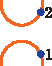
\includegraphics[scale=1]{CupCapDots.pdf}}}}}

\newcommand{\dbeta}{\mathord{\vcenter{\hbox{
\includegraphics[scale=1]{dbeta.pdf}}}}}
\newcommand{\dpsi}{\mathord{\vcenter{\hbox{
\includegraphics[scale=1]{dpsi.pdf}}}}}
\newcommand{\dblank}{\mathord{\vcenter{\hbox{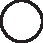
\includegraphics[scale=1]{dblank.pdf}}}}}





\newcommand{\SigmaDotDot}{\mathord{\vcenter{\hbox{
\includegraphics[scale=1]{SigmaDotDot.pdf}}}}}
\newcommand{\SigmaDotDotExchange}{\mathord{\vcenter{\hbox{
\includegraphics[scale=1]{SigmaDotDotExchange.pdf}}}}}
\newcommand{\TwoLine}{\mathord{\vcenter{\hbox{
\includegraphics[scale=1]{TwoLine.pdf}}}}}
\newcommand{\TwoLineDots}{\mathord{\vcenter{\hbox{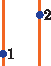
\includegraphics[scale=1]{TwoLineDots.pdf}}}}}


\newcommand{\RDotTwo}{\mathord{\vcenter{\hbox{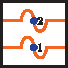
\includegraphics[scale=1]{RDotTwo.pdf}}}}}
\newcommand{\RDotTwoa}{\mathord{\vcenter{\hbox{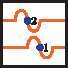
\includegraphics[scale=1]{RDotTwoa.pdf}}}}}
\newcommand{\RDotTwob}{\mathord{\vcenter{\hbox{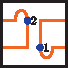
\includegraphics[scale=1]{RDotTwob.pdf}}}}}
\newcommand{\RDotTwoc}{\mathord{\vcenter{\hbox{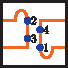
\includegraphics[scale=1]{RDotTwoc.pdf}}}}}

\newcommand{\FubeXXX}{\mathord{\vcenter{\hbox{
\includegraphics[scale=1]{EmptyTube.pdf}}}}}
\newcommand{\FubeXss}{\mathord{\vcenter{\hbox{
\includegraphics[scale=1]{OneLine.pdf}}}}}
\newcommand{\FubeXsds}{\mathord{\vcenter{\hbox{
\includegraphics[scale=1]{OneLineDot.pdf}}}}}



\newcommand{\AnnulusCut}{\mathord{\vcenter{\hbox{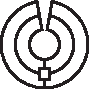
\includegraphics[scale=1]{AnnulusCut.pdf}}}}}
\newcommand{\AnnulusFlat}{\mathord{\vcenter{\hbox{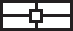
\includegraphics[scale=1]{AnnulusFlat.pdf}}}}}
\newcommand{\Disc}{\mathord{\vcenter{\hbox{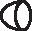
\includegraphics[scale=1]{Disc.pdf}}}}}
\newcommand{\RotatedTube}{\mathord{\vcenter{\hbox{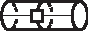
\includegraphics[scale=1]{RotatedTube.pdf}}}}}
\newcommand{\AnnulusGeneric}{\mathord{\vcenter{\hbox{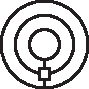
\includegraphics[scale=1]{AnnulusGeneric.pdf}}}}}



\newcommand{\FubeXXXA}{\mathord{\vcenter{\hbox{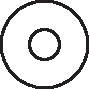
\includegraphics[scale=1]{EmptyTubeA.pdf}}}}}
\newcommand{\FubeXssA}{\mathord{\vcenter{\hbox{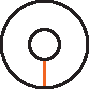
\includegraphics[scale=1]{OneLineA.pdf}}}}}
\newcommand{\FubeXsdsA}{\mathord{\vcenter{\hbox{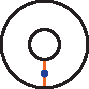
\includegraphics[scale=1]{OneLineDotA.pdf}}}}}

\newcommand{\FubesddXsA}{\mathord{\vcenter{\hbox{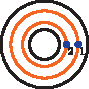
\includegraphics[scale=1]{FubesddXsA.pdf}}}}}

\newcommand{\RDotTwobA}{\mathord{\vcenter{\hbox{
\includegraphics[scale=1]{RDotTwobA.pdf}}}}}\newcommand{\RDotTwocA}{\mathord{\vcenter{\hbox{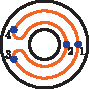
\includegraphics[scale=1]{RDotTwocA.pdf}}}}}


 
\newcommand{\Fubex}[2]{{\mathord{\ooalign{ \vphantom{$\Big|^2$}\cr\hidewidth\ensuremath{\scriptstyle{#2}}\hidewidth\cr$\vcenter{\hbox{$#1$}}$\cr
  \hidewidth\raise0ex\hbox{$\scale{1.2}{\VerticalSpace}$}\cr
  }}}}	




\newcommand{\TubeBC}{\mathord{\vcenter{\hbox{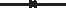
\includegraphics[scale=1]{TubeBC.pdf}}}}}

\newcommand{\TubeBCx}[1]{{\mathord{\ooalign{ \vphantom{$\Big|^2$}\cr\hidewidth\ensuremath{\scriptstyle{#1}}\hidewidth\cr$\vcenter{\hbox{$\scale{1}{\TubeBC}$}}$\cr
  \hidewidth\raise0ex\hbox{$\scale{.25}{\VerticalSpace}$}\cr
  }}}}	

\newcommand{\AnnulusBare}{\mathord{\vcenter{\hbox{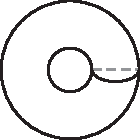
\includegraphics[scale=.6]{AnnulusBare.pdf}}}}}
\newcommand{\AnnularTube}{\mathord{\vcenter{\hbox{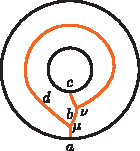
\includegraphics[scale=1]{AnnularTube.pdf}}}}}
\newcommand{\AnnularTubeNoIndex}{\mathord{\vcenter{\hbox{
\includegraphics[scale=1]{AnnularTubeNoIndex.pdf}}}}}
\newcommand{\AnnulusTubeTube}{\mathord{\vcenter{\hbox{
\includegraphics[scale=1]{AnnulusTubeTube.pdf}}}}}

\newcommand{\SAnnulusNoLabel}{\mathord{\vcenter{\hbox{
\includegraphics[scale=1]{SAnnulusNoLabel.pdf}}}}}
\newcommand{\TAnnulusNoLabel}{\mathord{\vcenter{\hbox{
\includegraphics[scale=1]{TAnnulusNoLabel.pdf}}}}}



\newcommand{\AnnulsLabel}[5]{\mathord{ 
\mkern2mu\overset{#3}{{\Annulusxprime{#1}{#2}}}\mkern2mu\raisebox{0ex}{$\scriptstyle{#4}$} }}

\newcommand*{\Annulus}[2]{{ #1 }
\kern-3.5em\raisebox{1ex}{ $\scriptstyle{#2}$} \kern2.6em} %Could change 0 to 1.2 to raise the B.

\newcommand*{\AnnulusP}[3]{{{\Annulus{#1}{#2}} }
\kern-.5em\raisebox{3.5ex}{ $\scriptstyle{#3}$} \kern.3em} %Could change 0 to 1.2 to raise the B.

\newcommand*{\AnnulusPx}[4]{\AnnulusP{#1}{#2}{#3}
\kern-3.6em\raisebox{-4.5ex}{ $\scriptstyle{#4}$} \kern2.6em} %Could change 0 to 1.2 to raise the B.

\newcommand*{\AnularTubex}[6]{\AnnulusPx{#1}{#2}{#3}{#4}
\kern-4em\raisebox{-4.5ex}{ $\overset{#6}{\underset{#5}{\vphantom{\Big|^2}}}$} \kern3em} %Could change 0 to 1.2 to raise the B.

\newcommand*{\TorusTubex}[6]{\AnnulusPx{#1}{#2}{#3}{#4}
\kern-4em\raisebox{-4.5ex}{ $\overset{#6}{\underset{#5}{\vphantom{\Big|^2}}}$} \kern3em} %Could change 0 to 1.2 to raise the B.

%\newcommand*{\AnnularTubex}[5]{\AnnulusPx{#1}{#2}{}{\; \; \;#3}
%\kern-3.9em\raisebox{-4.5ex}{ $\overset{#5}{\underset{#4}{\vphantom{\Big|^2}}}$} \kern2.7em} %Could change 0 to 1.2 to raise the B.



\newcommand{\SAnnulusx}[3]{\mathrel{\ooalign{$\SAnnulusNoLabel$\cr
  \hidewidth\raise5ex\hbox{$\scriptstyle{#3}\mkern1mu$}\cr
  \hidewidth\raise.8ex\hbox{$\scriptstyle{#2}\mkern63mu$}\cr
    \hidewidth\raise-3.8ex\hbox{$\scriptstyle{#1}\mkern39mu$}\cr
  }}}
  
  \newcommand{\TAnnulusx}[3]{\mathrel{\ooalign{$\TAnnulusNoLabel$\cr
  \hidewidth\raise5ex\hbox{$\scriptstyle{#3}\mkern1mu$}\cr
  \hidewidth\raise.8ex\hbox{$\scriptstyle{#2}\mkern63mu$}\cr
    \hidewidth\raise-4.9ex\hbox{$\scriptstyle{#1}\mkern51mu$}\cr
  }}}

\newcommand{\AnnularTubex}[6]{\mathrel{\ooalign{$#1$\cr
  \hidewidth\raise5ex\hbox{$\scriptstyle{#6}\mkern1mu$}\cr
  \hidewidth\raise.8ex\hbox{$\scriptstyle{#5}\mkern63mu$}\cr
  \hidewidth\raise-.9ex\hbox{$\scriptstyle{#3}\mkern68mu$}\cr
    \hidewidth\raise-4.5ex\hbox{$\scriptstyle{#4} \mkern50mu$}\cr
  \hidewidth\raise-7ex\hbox{$\scriptstyle{#2}\mkern68mu$}\cr
  }}}
  
%\newcommand{\AnnularTubexp}[9]{\mathrel{\ooalign{$#1$\cr
  %\hidewidth\raise5ex\hbox{$\scriptstyle{#9}\mkern1mu$}\cr
 %\hidewidth\raise.8ex\hbox{$\scriptstyle{#8}\mkern63mu$}\cr
 % \hidewidth\raise-3.4ex\hbox{$\scriptstyle{#7}\mkern68mu$}\cr
  %  \hidewidth\raise-5.1ex\hbox{$\scriptstyle{#6}\mkern80mu$}\cr
%  \hidewidth\raise-2.2ex\hbox{$\scriptstyle{#5}\mkern90mu$}\cr
 % \hidewidth\raise-.9ex\hbox{$\scriptstyle{#4}\mkern68mu$}\cr
%    \hidewidth\raise-4.5ex\hbox{$\scriptstyle{#3} \mkern50mu$}\cr
 % \hidewidth\raise-7ex\hbox{$\scriptstyle{#2}\mkern68mu$}\cr
 % }}}



\newcommand{\AnnularTubexp}[9]{\mathrel{\ooalign{$#1$\cr
  \hidewidth\raise5ex\hbox{$\scriptstyle{#9}\mkern1mu$}\cr
 \hidewidth\raise.8ex\hbox{$\scriptstyle{#8}\mkern63mu$}\cr
  \hidewidth\raise-3.7ex\hbox{$\scriptstyle{#7}\mkern50mu$}\cr
    \hidewidth\raise-5.1ex\hbox{$\scriptstyle{#6}\mkern57mu$}\cr
  \hidewidth\raise-2.2ex\hbox{$\scriptstyle{#5}\mkern90mu$}\cr
  \hidewidth\raise-.9ex\hbox{$\scriptstyle{#4}\mkern68mu$}\cr
    \hidewidth\raise-3.8ex\hbox{$\scriptstyle{#3} \mkern69mu$}\cr
  \hidewidth\raise-7ex\hbox{$\scriptstyle{#2}\mkern68mu$}\cr
  }}}


\newcommand{\SmallTorus}[3]{\mathrel{\ooalign{$#1$\cr
  \hidewidth\raise0ex\hbox{$\scriptstyle{#2}\mkern36mu$}\cr
    \hidewidth\raise-1.5ex\hbox{$\scriptstyle{#3}\mkern10mu$}\cr
  }}}
  
  
  \newcommand{\AnnulusTubeTubex}[6]{\mathrel{\ooalign{$#1$\cr
%  \hidewidth\raise5ex\hbox{$\scriptstyle{#7}\mkern1mu$}\cr
  \hidewidth\raise.8ex\hbox{$\scriptstyle{#6}\mkern65mu$}\cr
  \hidewidth\raise-.5ex\hbox{$\scriptstyle{#3}\mkern68mu$}\cr
    \hidewidth\raise-4.9ex\hbox{$\scriptstyle{#4} \mkern50mu$}\cr
     \hidewidth\raise-2.7ex\hbox{$\scriptstyle{#5} \mkern54mu$}\cr
  \hidewidth\raise-7.3ex\hbox{$\scriptstyle{#2}\mkern68mu$}\cr
  }}}
  


\newcommand{\TorusLocalRelationc}{\mathord{\vcenter{\hbox{
\includegraphics[scale=1]{TorusLocalRelationc.pdf}}}}}
\newcommand{\TorusLocalRelationb}{\mathord{\vcenter{\hbox{
\includegraphics[scale=1]{TorusLocalRelationb.pdf}}}}}
\newcommand{\TorusLocalRelationa}{\mathord{\vcenter{\hbox{
\includegraphics[scale=1]{TorusLocalRelationa.pdf}}}}}


\newcommand{\Dv}{\mathord{\vcenter{\hbox{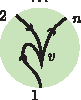
\includegraphics[scale=1]{Dv.pdf}}}}}
\newcommand{\Dfv}{\mathord{\vcenter{\hbox{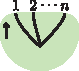
\includegraphics[scale=1]{Dfv.pdf}}}}}


\newcommand{\Horseshoe}{\mathord{\vcenter{\hbox{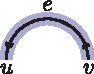
\includegraphics[scale=1]{Horseshoe.pdf}}}}}
\newcommand{\HorseshoeTwist}{\mathord{\vcenter{\hbox{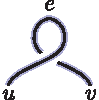
\includegraphics[scale=1]{HorseshoeTwist.pdf}}}}}
\newcommand{\euv}{\mathord{\vcenter{\hbox{\includegraphics[scale=1]{euv.pdf}}}}}
\newcommand{\chieuv}{\mathord{\vcenter{\hbox{\includegraphics[scale=1]{chieuv.pdf}}}}}

\newcommand{\IdempotentMTCNoLabel}{\mathord{\vcenter{\hbox{\includegraphics[scale=1]{IdempotentMTC.pdf}}}}}
\newcommand{\IdempBraid}[5]{\mathrel{\ooalign{$\IdempotentMTCNoLabel$\cr
  \hidewidth\raise-4.3ex\hbox{$\scriptstyle{#1}\mkern78mu$}\cr
    \hidewidth\raise-4.3ex\hbox{$\scriptstyle{#2}\mkern43mu$}\cr
        \hidewidth\raise-6.3ex\hbox{$\scriptstyle{#3}\mkern61mu$}\cr
        \hidewidth\raise4.1ex\hbox{$\scriptstyle{#4}\mkern25mu$}\cr
                \hidewidth\raise0ex\hbox{$\scriptstyle{#5}\mkern60mu$}\cr
          \hidewidth\raise0ex\hbox{$\scale{1.5}{\VerticalSpace}$}\cr
  }}}
  
\newcommand{\TorusBasisMTCNoLabel}{\mathord{\vcenter{\hbox{\includegraphics[scale=1]{TorusBasisMTC.pdf}}}}}
\newcommand{\TorusBraidBasis}[6]{\mathrel{\ooalign{$\TorusBasisMTCNoLabel$\cr
  \hidewidth\raise-4.3ex\hbox{$\scriptstyle{#1}\mkern78mu$}\cr
    \hidewidth\raise-4.3ex\hbox{$\scriptstyle{#2}\mkern40mu$}\cr
        \hidewidth\raise-6.3ex\hbox{$\scriptstyle{#3}\mkern61mu$}\cr
        \hidewidth\raise4.1ex\hbox{$\scriptstyle{#4}\mkern25mu$}\cr
                \hidewidth\raise0ex\hbox{$\scriptstyle{#5}\mkern58mu$}\cr
                                \hidewidth\raise4.7ex\hbox{$\scriptstyle{#6}\mkern0mu$}\cr
          \hidewidth\raise0ex\hbox{$\scale{1.5}{\VerticalSpace}$}\cr
  }}}
  
  \newcommand{\tcca}{\mathord{\vcenter{\hbox{\includegraphics[scale=1]{tcca.pdf}}}}}
    \newcommand{\tccb}{\mathord{\vcenter{\hbox{\includegraphics[scale=1]{tccb.pdf}}}}}
     \newcommand{\tccc}{\mathord{\vcenter{\hbox{\includegraphics[scale=1]{tccc.pdf}}}}}
      \newcommand{\tccd}{\mathord{\vcenter{\hbox{\includegraphics[scale=1]{tccd.pdf}}}}}
   
  
 


\newcommand{\TorusBasisMTCdl}{\mathord{\vcenter{\hbox{\includegraphics[scale=1]{TorusBasisMTCdl.pdf}}}}}
\newcommand{\TorusBasisMTCdr}{\mathord{\vcenter{\hbox{\includegraphics[scale=1]{TorusBasisMTCdr.pdf}}}}}
\newcommand{\TorusBasisMTCdd}{\mathord{\vcenter{\hbox{\includegraphics[scale=1]{TorusBasisMTCdd.pdf}}}}}
 
 \newcommand{\TorusBraidBasisd}[7]{\mathrel{\ooalign{$#7$\cr
  \hidewidth\raise-4.3ex\hbox{$\scriptstyle{#1}\mkern78mu$}\cr
    \hidewidth\raise-4.3ex\hbox{$\scriptstyle{#2}\mkern40mu$}\cr
        \hidewidth\raise-6.3ex\hbox{$\scriptstyle{#3}\mkern61mu$}\cr
        \hidewidth\raise4.1ex\hbox{$\scriptstyle{#4}\mkern25mu$}\cr
                \hidewidth\raise0ex\hbox{$\scriptstyle{#5}\mkern58mu$}\cr
                                \hidewidth\raise4.7ex\hbox{$\scriptstyle{#6}\mkern0mu$}\cr
          \hidewidth\raise0ex\hbox{$\scale{1.5}{\VerticalSpace}$}\cr
  }}}



\newcommand{\TaddownTubeNoLabel}{\mathord{\vcenter{\hbox{\includegraphics[scale=1]{TaddownTube.pdf}}}}}
\newcommand{\TadupTubeNoLabel}{\mathord{\vcenter{\hbox{\includegraphics[scale=1]{TadupTube.pdf}}}}}
\newcommand{\hTube}{\mathord{\vcenter{\hbox{\includegraphics[scale=1]{hTube.pdf}}}}}
\newcommand{\tTube}{\mathord{\vcenter{\hbox{\includegraphics[scale=1]{tTube.pdf}}}}}
\newcommand{\eTube}{\mathord{\vcenter{\hbox{\includegraphics[scale=1]{eTube.pdf}}}}}
\newcommand{\vTube}{\mathord{\vcenter{\hbox{\includegraphics[scale=1]{vTube.pdf}}}}}


\newcommand{\dota}{\mathord{\vcenter{\hbox{\includegraphics[scale=1]{dota.pdf}}}}}
\newcommand{\dotb}{\mathord{\vcenter{\hbox{\includegraphics[scale=1]{dotb.pdf}}}}}
\newcommand{\dotc}{\mathord{\vcenter{\hbox{\includegraphics[scale=1]{dotc.pdf}}}}}

\newcommand{\XTubeNoLabel}{\mathord{\vcenter{\hbox{\includegraphics[scale=1]{XTube.pdf}}}}}
\newcommand{\XTube}[2]{\mathrel{\ooalign{$\XTubeNoLabel$\cr
  \hidewidth\raise-2.5ex\hbox{$\scriptstyle{#2}\mkern28mu$}\cr
    \hidewidth\raise-2.9ex\hbox{$\scriptstyle{#1}\mkern50mu$}\cr
  }}}


\newcommand{\TaddownTube}[1]{\mathrel{\ooalign{$\TaddownTubeNoLabel$\cr
    \hidewidth\raise-2.8ex\hbox{$\scriptstyle{#1}\mkern30mu$}\cr
  }}}
  \newcommand{\TadupTube}[1]{\mathrel{\ooalign{$\TadupTubeNoLabel$\cr
    \hidewidth\raise-2.6ex\hbox{$\scriptstyle{#1}\mkern30mu$}\cr
  }}}
  
  \newcommand{\TorusNoLabels}{\mathord{\vcenter{\hbox{\includegraphics[scale=1]{TorusNoLabels.pdf}}}}}
\newcommand{\TorusNoLabelsx}[1]{\mathrel{\ooalign{$\TorusNoLabels$\cr
    \hidewidth\raise-2.8ex\hbox{$\scriptstyle{#1}\mkern30mu$}\cr
  }}}

\newcommand{\VerticalSpace}{\mathord{\vcenter{\hbox{\includegraphics[scale=1]{VerticalSpace.pdf}}}}}

\newcommand{\AddDat}[3]{\mathrel{\ooalign{  $#1$\cr
  \hidewidth\raise0ex\hbox{$\scriptstyle{#2}\mkern38mu$}\cr
  \hidewidth\raise0ex\hbox{${#3}\mkern0mu$}\cr
  \hidewidth\raise0ex\hbox{$\VerticalSpace$}\cr
  }}}
  
  \newcommand{\AddDatTorus}[3]{\mathrel{\ooalign{  $#1$\cr
  \hidewidth\raise0ex\hbox{$\scriptstyle{#2}\mkern38mu$}\cr
  \hidewidth\raise3.8ex\hbox{$\scriptstyle{#3}\mkern0mu$}\cr
  \hidewidth\raise0ex\hbox{$\VerticalSpace$}\cr
  }}}
  
    \newcommand{\AddDatTorusDot}[4]{\mathrel{\ooalign{  $#1$\cr
  \hidewidth\raise0ex\hbox{$\scriptstyle{#2}\mkern38mu$}\cr
  \hidewidth\raise3.8ex\hbox{$\scriptstyle{#3}\mkern0mu$}\cr
  \hidewidth\raise0ex\hbox{${#4}\mkern0mu$}\cr
  \hidewidth\raise0ex\hbox{$\VerticalSpace$}\cr
  }}}
  
  
  
 
  
   
  \newcommand{\TubeProductCoefficienta}{\mathord{\vcenter{\hbox{\includegraphics[scale=1]{TubeProductCoefficienta.pdf}}}}}
  \newcommand{\TubeProductCoefficientb}{\mathord{\vcenter{\hbox{\includegraphics[scale=1]{TubeProductCoefficientb.pdf}}}}}
  
    \newcommand{\ThetaSymbol}{\mathord{\vcenter{\hbox{\includegraphics[scale=1]{Theta.pdf}}}}}
 
   \newcommand{\ThetaSymbolx}[1]{\mathrel{\ooalign{$\ThetaSymbol$\cr
      \hidewidth\raise-1.3ex\hbox{$\scriptstyle{#1} \mkern0mu$}\cr
  }}}
  
  
    
  \newcommand{\TubeProductCoefficientbx}[2]{\mathrel{\ooalign{$\TubeProductCoefficientb \;\;\; $\cr
      \hidewidth\raise-.8ex\hbox{$\scriptstyle{#1} \mkern54mu$}\cr
      \hidewidth\raise-.8ex\hbox{$\scriptstyle{#2} \mkern6mu$}\cr
  }}}
  
  \newcommand{\TubeProductCoefficientax}[5]{\mathrel{\ooalign{$\TubeProductCoefficienta$\cr
      \hidewidth\raise-4.2ex\hbox{$\scriptstyle{#1} \mkern30mu$}\cr
      \hidewidth\raise-1.8ex\hbox{$\scriptstyle{#2} \mkern30mu$}\cr
  \hidewidth\raise6.1ex\hbox{$\scriptstyle{#3}\mkern44mu$}\cr
  \hidewidth\raise2.05ex\hbox{$\scriptstyle{#4}\mkern82mu$}\cr
    \hidewidth\raise3.2ex\hbox{$\scriptstyle{#5}\mkern3mu$}\cr
  }}}

  

  
    
\newcommand{\tubex}[8]{#1 \left(\substack{#8\\ \\ #5\\ } \; \substack{#4\\ #3\\ #2\\ }\; \substack{ #7 \\ #6} \right)}
%\newcommand*{\SmallTorus}[3]{\kern 2.05 em\raisebox{0ex}{ $\scriptstyle{#2}$} \kern-2.05em{ #1 } 
%\kern-1.1em\raisebox{-1.5ex}{$\scriptstyle{#3}$} \kern1.1em} %Could change 0 to 1.2 to raise the B.


%\newcommand*{\Tubex}[2]{{ \AnnularTube }
%\kern-3.5em\raisebox{1ex}{ $\scriptstyle{#2}$} \kern3.5em} %Could change 0 to 1.2 to raise the B.


%\newcommand{\BWfour}[5]{\mathord{ \raisebox{0.2ex}{$\scriptstyle{#2}$}\mkern2mu\overset{#3}{\underset{#4}{#1}}\mkern2mu\raisebox{0.2ex}{$\scriptstyle{#5}$} }}




\newcommand{\FubesXs}{\mathord{\vcenter{\hbox{\includegraphics[scale=1,angle=90,origin=c]{OneLine.pdf}}}}}
\newcommand{\FubesdXs}{\mathord{\vcenter{\hbox{\includegraphics[scale=1]{FubesdXs.pdf}}}}}

\newcommand{\FubessX}{\mathord{\vcenter{\hbox{\includegraphics[scale=1]{FubessX.pdf}}}}}
\newcommand{\FubessdX}{\mathord{\vcenter{\hbox{\includegraphics[scale=1]{FubessdX.pdf}}}}}

\newcommand{\FubesdXsA}{\mathord{\vcenter{\hbox{\includegraphics[scale=1]{FubesdXsA.pdf}}}}}
\newcommand{\FubessXA}{\mathord{\vcenter{\hbox{\includegraphics[scale=1]{FubessXA.pdf}}}}}
\newcommand{\FubessdXA}{\mathord{\vcenter{\hbox{\includegraphics[scale=1]{FubessdXA.pdf}}}}}


\newcommand{\FubesXsA}{\mathord{\vcenter{\hbox{\includegraphics[scale=1]{FubesXshA.pdf}}}}}
\newcommand{\FubesXsa}{\mathord{\vcenter{\hbox{\includegraphics[scale=1]{FubesXsa.pdf}}}}}
\newcommand{\FubesXsb}{\mathord{\vcenter{\hbox{\includegraphics[scale=1]{FubesXsb.pdf}}}}}
\newcommand{\FubesXsc}{\mathord{\vcenter{\hbox{\includegraphics[scale=1]{FubesXsc.pdf}}}}}


\newcommand{\FubesXscA}{\mathord{\vcenter{\hbox{\includegraphics[scale=1]{FubeXscA.pdf}}}}}
\newcommand{\FubesXsbA}{\mathord{\vcenter{\hbox{\includegraphics[scale=1]{FubeXsbA.pdf}}}}}
\newcommand{\FubesXsaA}{\mathord{\vcenter{\hbox{\includegraphics[scale=1]{FubeXsaA.pdf}}}}}






\newcommand{\qqo}{\mathord{\vcenter{\hbox{\includegraphics[scale=.4]{qq1.pdf}}}}}
\newcommand{\qtqo}{\mathord{\vcenter{\hbox{\includegraphics[scale=.4]{qtq1.pdf}}}}}
\newcommand{\qqto}{\mathord{\vcenter{\hbox{\includegraphics[scale=.4]{qqt1.pdf}}}}}
\newcommand{\qtqto}{\mathord{\vcenter{\hbox{\includegraphics[scale=.4]{qtqt1.pdf}}}}}
\newcommand{\qqm}{\mathord{\vcenter{\hbox{\includegraphics[scale=.4]{qqm.pdf}}}}}
\newcommand{\qtqm}{\mathord{\vcenter{\hbox{\includegraphics[scale=.4]{qtqm.pdf}}}}}
\newcommand{\qqtm}{\mathord{\vcenter{\hbox{\includegraphics[scale=.4]{qqtm.pdf}}}}}
\newcommand{\qtqtm}{\mathord{\vcenter{\hbox{\includegraphics[scale=.4]{qtqtm.pdf}}}}}

\newcommand{\PantsPAP}{\mathord{\vcenter{\hbox{\includegraphics[scale=0.7]{PantsPAP.pdf}}}}}
\newcommand{\PantsPAsP}{\mathord{\vcenter{\hbox{\includegraphics[scale=0.7]{PantsPAsP.pdf}}}}}

\newcommand{\PantsPsdAP}{\mathord{\vcenter{\hbox{\includegraphics[scale=0.7]{PantsPsdAP.pdf}}}}}
\newcommand{\PantsPsdAsP}{\mathord{\vcenter{\hbox{\includegraphics[scale=0.7]{PantsPsdAsP.pdf}}}}}



\newcommand{\PantsPPA}{\mathord{\vcenter{\hbox{\includegraphics[scale=0.7]{PantsPPA.pdf}}}}}
\newcommand{\PantsPPAs}{\mathord{\vcenter{\hbox{\includegraphics[scale=0.7]{PantsPPAs.pdf}}}}}

\newcommand{\PantsAsAshAsvt}{\mathord{\vcenter{\hbox{\includegraphics[scale=0.7]{PantsAsAshAsvt.pdf}}}}}
\newcommand{\PantsAstAAs}{\mathord{\vcenter{\hbox{\includegraphics[scale=0.7]{PantsAstAAs.pdf}}}}}

\newcommand{\PantsAstAshAs}{\mathord{\vcenter{\hbox{\includegraphics[scale=0.7]{PantsAstAshAs.pdf}}}}}
\newcommand{\PantsAsAshAs}{\mathord{\vcenter{\hbox{\includegraphics[scale=0.7]{PantsAsAshAs.pdf}}}}}
\newcommand{\PantsAsAAs}{\mathord{\vcenter{\hbox{\includegraphics[scale=0.7]{PantsAsAAs.pdf}}}}}

\newcommand{\Pantssvtsvtsh}{\mathord{\vcenter{\hbox{\includegraphics[scale=.7,origin=c]{Pantssvtsvtsh.pdf}}}}}
\newcommand{\Pantssvtsvsh}{\mathord{\vcenter{\hbox{\includegraphics[scale=.7,angle=0,origin=c]{Pantssvtsvsh.pdf}}}}}
\newcommand{\Pantssvsvtsh}{\mathord{\vcenter{\hbox{\includegraphics[scale=.7,angle=0,origin=c]{Pantssvsvtsh.pdf}}}}}
\newcommand{\Pantssvsvsh}{\mathord{\vcenter{\hbox{\includegraphics[scale=.7,angle=0,origin=c]{Pantssvsvsh.pdf}}}}}
\newcommand{\PantssvtsvtX}{\mathord{\vcenter{\hbox{\includegraphics[scale=.7,angle=0,origin=c]{PantssvtsvtX.pdf}}}}}
\newcommand{\PantssvtsvX}{\mathord{\vcenter{\hbox{\includegraphics[scale=.7,angle=0,origin=c]{PantssvtsvX.pdf}}}}}
%\newcommand{\PantssvtsvX}{\mathord{\vcenter{\hbox{\includegraphics[scale=.7,angle=0,origin=c]{PantssvtsvX.pdf}}}}}
\newcommand{\PantssvsvtX}{\mathord{\vcenter{\hbox{\includegraphics[scale=.7,angle=0,origin=c]{PantssvsvtX.pdf}}}}}
\newcommand{\PantssvsvX}{\mathord{\vcenter{\hbox{\includegraphics[scale=.7,angle=0,origin=c]{PantssvsvX.pdf}}}}}

\newcommand{\PantssvtXsvd}{\mathord{\vcenter{\hbox{\includegraphics[scale=.7,angle=0,origin=c]{PantssvtXsvd.pdf}}}}}
\newcommand{\Pantssvtshsvd}{\mathord{\vcenter{\hbox{\includegraphics[scale=.7,angle=0,origin=c]{Pantssvtshsvd.pdf}}}}}
\newcommand{\Pantssvshsvd}{\mathord{\vcenter{\hbox{\includegraphics[scale=.7,angle=0,origin=c]{Pantssvshsvd.pdf}}}}}
\newcommand{\PantssvXsvd}{\mathord{\vcenter{\hbox{\includegraphics[scale=.7,angle=0,origin=c]{PantssvXsvd.pdf}}}}}

\newcommand{\PantssvtXsvt}{\mathord{\vcenter{\hbox{\includegraphics[scale=.7,angle=0,origin=c]{PantssvtXsvt.pdf}}}}}
\newcommand{\PantssvXsvt}{\mathord{\vcenter{\hbox{\includegraphics[scale=.7,angle=0,origin=c]{PantssvXsvt.pdf}}}}}

\newcommand{\PantssvtXsv}{\mathord{\vcenter{\hbox{\includegraphics[scale=.7,angle=0,origin=c]{PantssvtXsv.pdf}}}}}



%%%%%%%%%%%%%%%%%%%%%%%%%%%%%%%%%%%%%%%%%%%%%%%%
%%%%%%%%%%%%%%%%%%%%%%%%%%%%%%%%%%%%%%%%%%%%%%%%
\newcommand{\PantssvXsvdA}{\mathord{\vcenter{\hbox{\includegraphics[scale=.8,angle=0,origin=c]{PantssvXsvdA.pdf}}}}}
\newcommand{\PantssvtXsvdA}{\mathord{\vcenter{\hbox{\includegraphics[scale=.8,angle=0,origin=c]{PantssvtXsvdA.pdf}}}}}
\newcommand{\PantssvtshsvdA}{\mathord{\vcenter{\hbox{\includegraphics[scale=.8,angle=0,origin=c]{PantssvtshsvdA.pdf}}}}}
\newcommand{\PantssvshsvdA}{\mathord{\vcenter{\hbox{\includegraphics[scale=.8,angle=0,origin=c]{PantssvshsvdA.pdf}}}}}
\newcommand{\PantsPsdAsPA}{\mathord{\vcenter{\hbox{\includegraphics[scale=.8,angle=0,origin=c]{PantsPsdAsPA.pdf}}}}}
\newcommand{\PantsPsdAPA}{\mathord{\vcenter{\hbox{\includegraphics[scale=.8,angle=0,origin=c]{PantsPsdAPA.pdf}}}}}
\newcommand{\PantsPPAsA}{\mathord{\vcenter{\hbox{\includegraphics[scale=.8,angle=0,origin=c]{PantsPPAsA.pdf}}}}}
\newcommand{\PantsPPAA}{\mathord{\vcenter{\hbox{\includegraphics[scale=.8,angle=0,origin=c]{PantsPPAA.pdf}}}}}
\newcommand{\PantsPAsPA}{\mathord{\vcenter{\hbox{\includegraphics[scale=.8,angle=0,origin=c]{PantsPAsPA.pdf}}}}}
\newcommand{\PantsPAPA}{\mathord{\vcenter{\hbox{\includegraphics[scale=.8,angle=0,origin=c]{PantsPAPA.pdf}}}}}
\newcommand{\PantsAstAAsA}{\mathord{\vcenter{\hbox{\includegraphics[scale=.8,angle=0,origin=c]{PantsAstAAsA.pdf}}}}}
\newcommand{\PantsAsAshAsvtA}{\mathord{\vcenter{\hbox{\includegraphics[scale=.8,angle=0,origin=c]{PantsAsAshAsvtA.pdf}}}}}
\newcommand{\PantsNNda}{\mathord{\vcenter{\hbox{\includegraphics[scale=.8,angle=0,origin=c]{PantsNNda.pdf}}}}}
\newcommand{\PantsNNd}{\mathord{\vcenter{\hbox{\includegraphics[scale=.8,angle=0,origin=c]{PantsNNd.pdf}}}}}
%%%%%%%%%%%%%%%%%%%%%%%%%%%%%%%%%%%%%%%%%%%%%%%%
%%%%%%%%%%%%%%%%%%%%%%%%%%%%%%%%%%%%%%%%%%%%%%%%

\newcommand{\TwoLinedotdot}{\mathord{\vcenter{\hbox{\includegraphics[scale=1.5,angle=0,origin=c]{TwoLinedotdot.pdf}}}}}

\newcommand{\Id}{\mathord{\vcenter{\hbox{\includegraphics[scale=1.5,angle=0,origin=c]{Id.pdf}}}}}

\newcommand{\CupSigmadot}{\mathord{\vcenter{\hbox{\includegraphics[scale=1.5,angle=0,origin=c]{Cupdot.pdf}}}}}

\newcommand{\CupSigma}{\mathord{\vcenter{\hbox{\includegraphics[scale=1.5,angle=0,origin=c]{Cup.pdf}}}}}

\newcommand{\StaggaredGSOdd}{\mathord{\vcenter{\hbox{\includegraphics[scale=1.5,angle=0,origin=c]{StaggaredGSOdd.pdf}}}}}
\newcommand{\StaggaredGSEven}{\mathord{\vcenter{\hbox{\includegraphics[scale=1.5,angle=0,origin=c]{StaggeredGSEven.pdf}}}}}

\newcommand{\StaggaredGSEvenR}{\mathord{\vcenter{\hbox{\reflectbox{\includegraphics[scale=1.5,angle=0,origin=c]{StaggeredGSEven.pdf}}}}}}





\newcommand{\VxsdsY}{\mathord{\vcenter{\hbox{\includegraphics[scale=0.3,angle=0,origin=c]{Vxsds.pdf}}}}}
\newcommand{\VsdxsY}{\mathord{\vcenter{\hbox{\includegraphics[scale=0.3,angle=0,origin=c]{Vsdxs.pdf}}}}}
\newcommand{\VtssdxY}{\mathord{\vcenter{\hbox{\includegraphics[scale=0.3,angle=0,origin=c]{Vtssdx.pdf}}}}}

\newcommand{\Vssdx}{\mathord{\vcenter{\hbox{\includegraphics[scale=0.3,angle=0,origin=c]{Vssdx.pdf}}}}}
\newcommand{\Vxsds}{\mathord{\vcenter{\hbox{\reflectbox{\includegraphics[scale=0.3,angle=0,origin=c]{Vssdx.pdf}}}}}}

\newcommand{\Vssx}{\mathord{\vcenter{\hbox{\includegraphics[scale=0.3,angle=0,origin=c]{Vssx.pdf}}}}}
\newcommand{\Vxss}{\mathord{\vcenter{\hbox{\reflectbox{\includegraphics[scale=0.3,angle=0,origin=c]{Vssx.pdf}}}}}}

\newcommand{\Vsxs}{\mathord{\vcenter{\hbox{\includegraphics[scale=0.3,angle=0,origin=c]{Vsxs.pdf}}}}}
\newcommand{\Vsxsd}{\mathord{\vcenter{\hbox{\includegraphics[scale=0.3,angle=0,origin=c]{Vsxsd.pdf}}}}}

\newcommand{\VsxsY}{\mathord{\vcenter{\hbox{\includegraphics[scale=0.3,angle=180,origin=c]{Vsxs.pdf}}}}}
\newcommand{\VssxY}{\mathord{\vcenter{\hbox{\includegraphics[scale=0.3,angle=180,origin=c]{Vssx.pdf}}}}}
\newcommand{\VxssY}{\mathord{\vcenter{\hbox{\reflectbox{\includegraphics[scale=0.3,angle=180,origin=c]{Vssx.pdf}}}}}}

\newcommand{\PsiFermion}{\mathord{\vcenter{\hbox{\includegraphics[scale=1.5]{PsiFermion.pdf}}}}}
\newcommand{\PsiFermionTwist}{\mathord{\vcenter{\hbox{\includegraphics[scale=1.5]{PsiFermionTwist.pdf}}}}}

\newcommand{\TwoFermion}{\mathord{\vcenter{\hbox{\includegraphics[scale=1.5]{TwoFermion.pdf}}}}}
\newcommand{\TwoFermionExchange}{\mathord{\vcenter{\hbox{\includegraphics[scale=1.5]{TwoFermionExchange.pdf}}}}}
\newcommand{\TwoFermionNoLabels}{\mathord{\vcenter{\hbox{\includegraphics[scale=1.5]{TwoFermion_nolabels.pdf}}}}}
\newcommand{\TwoFermionExchangeNoLabels}{\mathord{\vcenter{\hbox{\includegraphics[scale=1.5]{TwoFermionExchange_nolabels.pdf}}}}}


\newcommand{\Spin}{\mathord{\vcenter{\hbox{\includegraphics[scale=1.5]{Spin.pdf}}}}}
\newcommand{\PsiIdentity}{\mathord{\vcenter{\hbox{\includegraphics[scale=1.5]{PsiIdentity.pdf}}}}}

\newcommand{\TwoPsiExchange}{\mathord{\vcenter{\hbox{\includegraphics[scale=1.5]{TwoPsiExchange.pdf}}}}}
\newcommand{\TwoPsiIdentity}{\mathord{\vcenter{\hbox{\includegraphics[scale=1.5]{TwoPsiIdentity.pdf}}}}}


\newcommand{\PsiEnd}{\mathord{\vcenter{\hbox{\includegraphics[scale=1.5]{PsiEnd.pdf}}}}}
\newcommand{\PsiEndExchange}{\mathord{\vcenter{\hbox{\includegraphics[scale=1.5]{PsiEndExchange.pdf}}}}}

\newcommand{\DotSlidea}{\mathord{\vcenter{\hbox{\includegraphics[scale=1]{DotSlidea.pdf}}}}}
\newcommand{\DotSlideb}{\mathord{\vcenter{\hbox{\includegraphics[scale=1]{DotSlideb.pdf}}}}}
\newcommand{\DotSlidec}{\mathord{\vcenter{\hbox{\includegraphics[scale=1]{DotSlidec.pdf}}}}}
\newcommand{\DotSlided}{\mathord{\vcenter{\hbox{\includegraphics[scale=1]{DotSlided.pdf}}}}}

\newcommand{\QCapDotL}{\mathord{\vcenter{\hbox{\includegraphics[scale=1]{QDotslide.pdf}}}}}
\newcommand{\QCupDotR}{\mathord{\vcenter{\hbox{\includegraphics[scale=1,angle=180,origin=c]{QDotslide.pdf}}}}}
\newcommand{\QCapDotR}{\mathord{\vcenter{\hbox{\reflectbox{\includegraphics[scale=1]{QDotslide.pdf}}}}}}
\newcommand{\QCupDotL}{\mathord{\vcenter{\hbox{\reflectbox{\includegraphics[scale=1,angle=180,origin=c]{QDotslide.pdf}}}}}}

\newcommand{\TwodotCap}{\mathord{\vcenter{\hbox{\includegraphics[scale=1]{TwodotCap.pdf}}}}}
\newcommand{\TwodotCup}{\mathord{\vcenter{\hbox{\includegraphics[scale=1]{TwodotCup.pdf}}}}}


\newcommand{\Bpa}{\mathord{\vcenter{\hbox{\includegraphics[scale=1]{Bpa.pdf}}}}}
\newcommand{\Bpb}{\mathord{\vcenter{\hbox{\includegraphics[scale=1]{Bpb.pdf}}}}}
\newcommand{\Bpc}{\mathord{\vcenter{\hbox{\includegraphics[scale=1]{Bpc.pdf}}}}}
\newcommand{\Bpd}{\mathord{\vcenter{\hbox{\includegraphics[scale=1]{Bpd.pdf}}}}}
\newcommand{\Bpe}{\mathord{\vcenter{\hbox{\includegraphics[scale=1]{Bpe.pdf}}}}}
\newcommand{\Bpf}{\mathord{\vcenter{\hbox{\includegraphics[scale=1]{Bpf.pdf}}}}}
\newcommand{\Bpg}{\mathord{\vcenter{\hbox{\includegraphics[scale=1]{Bpg.pdf}}}}}
\newcommand{\Bph}{\mathord{\vcenter{\hbox{\includegraphics[scale=1]{Bph.pdf}}}}}
\newcommand{\Bpi}{\mathord{\vcenter{\hbox{\includegraphics[scale=1]{Bpi.pdf}}}}}

\newcommand{\LocalRelationLeft}{\mathord{\vcenter{\hbox{\includegraphics[scale=1]{LocalRelationLeft.pdf}}}}}
\newcommand{\LocalRelationRight}{\mathord{\vcenter{\hbox{\includegraphics[scale=1]{LocalRelationRight.pdf}}}}}
\newcommand{\LocalRelationUp}{\mathord{\vcenter{\hbox{\includegraphics[scale=1]{LocalRelationUp.pdf}}}}}
\newcommand{\LocalRelationDown}{\mathord{\vcenter{\hbox{\includegraphics[scale=1]{LocalRelationDown.pdf}}}}}

\newcommand{\PlaquettePrime}{\mathord{\vcenter{\hbox{\includegraphics[scale=1]{PlaquettePrime.pdf}}}}}

%\newcommand{\ycenter}{\mathord{\vcenter{\hbox{\includegraphics[scale=1.3]{ycenter.pdf}}}}}
%\newcommand{\ex}{\mathord{\vcenter{\hbox{\includegraphics[scale=1.3]{ex.pdf}}}}}
%\newcommand{\ey}{\mathord{\vcenter{\hbox{\includegraphics[scale=1.3]{ey.pdf}}}}}
%\newcommand{\eone}{\mathord{\vcenter{\hbox{\includegraphics[scale=1.3]{eone.pdf}}}}}

\newcommand{\ebox}{\mathord{\vcenter{\hbox{\includegraphics[scale=1.3]{ycenterNoLabel.pdf}}}}}
\newcommand{\ex}{\mathord{\vcenter{\hbox{\includegraphics[scale=1.3]{exNoLabel.pdf}}}}}
\newcommand{\ey}{\mathord{\vcenter{\hbox{\includegraphics[scale=1.3]{eyNoLabel.pdf}}}}}
\newcommand{\eone}{\mathord{\vcenter{\hbox{\includegraphics[scale=1.3]{eoneNoLabel.pdf}}}}}
\newcommand{\egeneral}{\mathord{\vcenter{\hbox{\includegraphics[scale=1.3]{egeneral.pdf}}}}}

\newcommand{\CTwoFusion}{\mathord{\vcenter{\hbox{\includegraphics[scale=1]{CTwoFusion.pdf}}}}}
\newcommand{\IdempEnd}{\mathord{\vcenter{\hbox{\includegraphics[scale=1]{IdempEnd.pdf}}}}}

\newcommand{\qqmbraida}{\mathord{\vcenter{\hbox{\includegraphics[scale=1]{qqmbraida.pdf}}}}}
\newcommand{\qqmbraidb}{\mathord{\vcenter{\hbox{\includegraphics[scale=1]{qqmbraidb.pdf}}}}}
\newcommand{\qqmbraidc}{\mathord{\vcenter{\hbox{\includegraphics[scale=1]{qqmbraidc.pdf}}}}}

\newcommand{\mmmbraida}{\mathord{\vcenter{\hbox{\includegraphics[scale=1]{mmmbraida.pdf}}}}}
\newcommand{\mmmbraidb}{\mathord{\vcenter{\hbox{\includegraphics[scale=1]{mmmbraidb.pdf}}}}}
\newcommand{\mmmbraidc}{\mathord{\vcenter{\hbox{\includegraphics[scale=1]{mmmbraidc.pdf}}}}}


\newcommand{\qqmbraidaOdd}{\mathord{\vcenter{\hbox{\includegraphics[scale=1]{qqmbraidaOdd.pdf}}}}}
\newcommand{\qqmbraidbOdd}{\mathord{\vcenter{\hbox{\includegraphics[scale=1]{qqmbraidbOdd.pdf}}}}}
\newcommand{\qqmbraidcOdd}{\mathord{\vcenter{\hbox{\includegraphics[scale=1]{qqmbraidcOdd.pdf}}}}}

\newcommand{\qqmbraidOdda}{\mathord{\vcenter{\hbox{\includegraphics[scale=1]{qqmbraidOdda.pdf}}}}}
\newcommand{\qqmbraidOddb}{\mathord{\vcenter{\hbox{\includegraphics[scale=1]{qqmbraidOddb.pdf}}}}}
\newcommand{\qqmbraidOddc}{\mathord{\vcenter{\hbox{\includegraphics[scale=1]{qqmbraidOddc.pdf}}}}}
\newcommand{\qqmbraidOddd}{\mathord{\vcenter{\hbox{\includegraphics[scale=1]{qqmbraidOddd.pdf}}}}}


%%
%%
%This one is used for pre-subscripts.
\usepackage{leftidx}
\newcommand{\overunderset}[3]{\overset{#3}{\underset{#2}{#1}}}

  \newcommand{\halfbraid}[4]{\mathrel{\ooalign{
  \vphantom{$\Big|^2$}  
  $\leftidx{_{#2}}{\overunderset{#1}{#3}{#3}}{^{#2}}$\cr
   \hidewidth \hbox{$\scriptstyle{#4}\mkern32mu$}\cr
     \hidewidth\raise0ex\hbox{$\scale{1.5}{\VerticalSpace}$}\cr
 }}}

 
  \newcommand{\halfbraidHex}[5]{\mathrel{\ooalign{
  \vphantom{$\Big|^2$}  
  $\leftidx{_{#2}}{\overunderset{#1}{#3}{#4 \quad \; \; \; #5}}{^{#2}}$\cr
     \hidewidth\raise0ex\hbox{$\scale{2.5}{\VerticalSpace}$}\cr
 }}}
%%
%%


%  \newcommand{\halfbraid}[4]{\mathrel{\ooalign{
 % \vphantom{$\Big|^2$}  
%  $\sideset{_{#2}}{}\overunderset{#1}{#2}{#3}$\cr
 %  \hidewidth \hbox{$\scriptstyle{#4}\mkern32mu$}\cr
 %    \hidewidth\raise0ex\hbox{$\scale{1.5}{\VerticalSpace}$}\cr
% }}}
 
%  \newcommand{\halfbraid}[4]{\mathrel{\ooalign{
 % \vphantom{$\Big|^2$}  
 % $\sideset{_{#2}}{}{\overset{#3}{\underset{#3}{#1}}^{#2}}$\cr
  % \hidewidth \hbox{$\scriptstyle{#4}\mkern32mu$}\cr
   %  \hidewidth\raise0ex\hbox{$\scale{1.5}{\VerticalSpace}$}\cr
 %}}}


\newcommand{\HalfBraidHexa}{\mathord{\vcenter{\hbox{\includegraphics[scale=1.3]{HalfBraidHexa.pdf}}}}}
\newcommand{\HalfBraidHexb}{\mathord{\vcenter{\hbox{\includegraphics[scale=1.3]{HalfBraidHexb.pdf}}}}}
 
 % \newcommand{\halfbraidHex}[5]{\mathrel{\ooalign{
 % \vphantom{$\Big|^2$}  
 % $\sideset{_{#2}}{}{\overset{#4 \quad \;  \; \; #5}{\underset{#3}{#1}}^{#2}}$\cr
  %     \hidewidth\raise0ex\hbox{$\scale{2.5}{\VerticalSpace}$}\cr
% }}}



\newcommand{\TubeXb}{\mathord{\vcenter{\hbox{\includegraphics[scale=1]{TubeXb.pdf}}}}}
\newcommand{\TubeXa}{\mathord{\vcenter{\hbox{\includegraphics[scale=1]{TubeXa.pdf}}}}}
\newcommand{\TubeXtwist}{\mathord{\vcenter{\hbox{\includegraphics[scale=1]{TubeXtwist.pdf}}}}}
\newcommand{\Tubeidx}{\mathord{\vcenter{\hbox{\includegraphics[scale=1]{Tubeidx.pdf}}}}}
\newcommand{\Tubexloop}{\mathord{\vcenter{\hbox{\includegraphics[scale=1]{Tubexloop.pdf}}}}}
\newcommand{\TubeEmpty}{\mathord{\vcenter{\hbox{\includegraphics[scale=1]{TubeEmpty.pdf}}}}}

\newcommand{\xOdd}{\mathord{\vcenter{\hbox{\includegraphics[scale=1]{xOdd.pdf}}}}}
\newcommand{\tOdd}{\mathord{\vcenter{\hbox{\includegraphics[scale=1]{tOdd.pdf}}}}}
\newcommand{\vOdd}{\mathord{\vcenter{\hbox{\includegraphics[scale=1]{vOdd.pdf}}}}}
\newcommand{\hOdd}{\mathord{\vcenter{\hbox{\includegraphics[scale=1]{hOdd.pdf}}}}}

\newcommand{\TorusBasisa}{\mathord{\vcenter{\hbox{\includegraphics[scale=1]{TorusBasisa.pdf}}}}}
\newcommand{\TorusBasisb}{\mathord{\vcenter{\hbox{\includegraphics[scale=1]{TorusBasisb.pdf}}}}}
\newcommand{\STorusBasisa}{\mathord{\vcenter{\hbox{\includegraphics[scale=1]{STorusBasisa.pdf}}}}}

\newcommand{\scale}[2]{\scalebox{#1}{$#2$}}



\newcommand{\TubeXbv}{\mathord{\vcenter{\hbox{\includegraphics[scale=1]{TubeXbv.pdf}}}}}
\newcommand{\TubeXav}{\mathord{\vcenter{\hbox{\includegraphics[scale=1]{TubeXav.pdf}}}}}
\newcommand{\TubeXtwistv}{\mathord{\vcenter{\hbox{\includegraphics[scale=1]{TubeXtwistv.pdf}}}}}
\newcommand{\Tubeidxv}{\mathord{\vcenter{\hbox{\includegraphics[scale=1]{Tubeidxv.pdf}}}}}
\newcommand{\TubeEmptyv}{\mathord{\vcenter{\hbox{\includegraphics[scale=1]{TubeEmptyv.pdf}}}}}



\newcommand{\TorusQQQa}{\mathord{\vcenter{\hbox{\includegraphics[scale=1]{TorusQQQa.pdf}}}}}
\newcommand{\TorusQQQb}{\mathord{\vcenter{\hbox{\includegraphics[scale=1]{TorusQQQb.pdf}}}}}
\newcommand{\TorusQQQc}{\mathord{\vcenter{\hbox{\includegraphics[scale=1]{TorusQQQc.pdf}}}}}
\newcommand{\TorusQQQd}{\mathord{\vcenter{\hbox{\includegraphics[scale=1]{TorusQQQd.pdf}}}}}

\newcommand{\VSa}{\mathord{\vcenter{\hbox{\includegraphics[scale=1.3]{VSa.pdf}}}}}
\newcommand{\VSb}{\mathord{\vcenter{\hbox{\includegraphics[scale=1.3]{VSb.pdf}}}}}
\newcommand{\VSc}{\mathord{\vcenter{\hbox{\includegraphics[scale=1.3]{VSc.pdf}}}}}
\newcommand{\VSd}{\mathord{\vcenter{\hbox{\includegraphics[scale=1.3]{VSd.pdf}}}}}


\newcommand{\VNoLabel}{\mathord{\vcenter{\hbox{\includegraphics[scale=1.3]{VNoLabel.pdf}}}}}
\newcommand{\VVNoLabel}{\mathord{\vcenter{\hbox{\includegraphics[scale=1.3]{VVNolabel.pdf}}}}}

\newcommand{\DotX}{\mathord{\vcenter{\hbox{\includegraphics[scale=1.3]{DotX.pdf}}}}}
\newcommand{\DotY}{\mathord{\vcenter{\hbox{\includegraphics[scale=1.3]{DotY.pdf}}}}}
\newcommand{\DotZ}{\mathord{\vcenter{\hbox{\includegraphics[scale=1.3]{DotZ.pdf}}}}} 

\newcommand{\VVDotX}{\mathord{\vcenter{\hbox{\includegraphics[scale=1.3]{VVDotX.pdf}}}}}
\newcommand{\VVDotY}{\mathord{\vcenter{\hbox{\includegraphics[scale=1.3]{VVDotY.pdf}}}}}
\newcommand{\VVDotZ}{\mathord{\vcenter{\hbox{\includegraphics[scale=1.3]{VVDotZ.pdf}}}}} 

\newcommand{\VertexInnerProduct}{\mathord{\vcenter{\hbox{\includegraphics[scale=1.3]{VertexInnerProduct.pdf}}}}}


\newcommand{\EdgeVecNoLabel}{\mathord{\vcenter{\hbox{\includegraphics[scale=1.3]{EdgeVec.pdf}}}}}
\newcommand{\EdgeVec}[2]{\leftidx{_{#1\; }}{\EdgeVecNoLabel}{_{\; #2}}}


%pitchforks
%%%%%%%%%%%%%%%%%%%%%%%%%%%%%%%%%%%%%%%%%%%%%
\newcommand{\PitchForkNoLabel}{\mathord{\vcenter{\hbox{\includegraphics[scale=1.3]{PitchForkNoLabel.pdf}}}}}
\newcommand{\PitchForkNoLabelas}{\mathord{\vcenter{\hbox{\includegraphics[scale=1.3]{PitchForkNoLabeladual.pdf}}}}}

\newcommand{\PitchForkWithEdge}{\mathord{\vcenter{\hbox{\includegraphics[scale=1.3]{PitchForkWithEdge.pdf}}}}}


\newcommand{\PitchFork}[4]{\overset{#2}{\leftidx{_{}^{#1}}{\underset{#4}{\PitchForkNoLabel}}{^{#3}}}}
\newcommand{\PitchForkas}[4]{\underset{#4}{\overset{#2}{\leftidx{_{}^{#1}}{\PitchForkNoLabelas}{^{#3}}}}}

%odd pitchforks
%\newcommand{\PitchForkNoLabelleft}{\mathord{\vcenter{\hbox{\includegraphics[scale=1.3]{PitchForkNoLabel_leftdot.pdf}}}}}
%\newcommand{\PitchForkNoLabelright}{\mathord{\vcenter{\hbox{\includegraphics[scale=1.3]{PitchForkNoLabel_rightdot.pdf}}}}}

%\newcommand{\PitchForkLeftDot}[4]{\overset{#2}{\leftidx{_{}^{#1}}{\underset{#4}{\PitchForkNoLabelleft}}{^{#3}}}}
%\newcommand{\PitchForkRightDot}[4]{\overset{#2}{\leftidx{_{}^{#1}}{\underset{#4}{\PitchForkNoLabelright}}{^{#3}}}}
%%%%%%%%%%%%%%%%%%%%%%%%%%%%%%%%%

 
     \newcommand{\VNoLabelDot}[1]{\mathrel{\ooalign{  $\VNoLabel$\cr
  \hidewidth\raise0ex\hbox{${#1}\mkern0mu$}\cr %dot
%     \hidewidth\raise0ex\hbox{$\scale{0.9}{\VerticalSpace}$}\cr
%  \hidewidth\raise0ex\hbox{$\VerticalSpace$}\cr
  }}}
  
       \newcommand{\VVNoLabelDot}[1]{\mathrel{\ooalign{  $\VVNoLabel$\cr
  \hidewidth\raise0ex\hbox{${#1}\mkern0mu$}\cr %dot
%     \hidewidth\raise0ex\hbox{$\scale{0.9}{\VerticalSpace}$}\cr
%  \hidewidth\raise0ex\hbox{$\VerticalSpace$}\cr
  }}}
 
%   $\leftidx{^{#1}}{\underset{\VNoLabel}{#3}}{^{#2}}$\cr
 %\psi^{ab}_{c,\mu}, \DotX

    \newcommand{\Vx}[4]{\mathrel{\ooalign{  $\overset{#1\kern2.8em #2}{\underset{#3}{\VNoLabel}}$\cr
  \hidewidth\raise0ex\hbox{${#4}\mkern12mu$}\cr 
  }}}

    \newcommand{\VDotx}[5]{\mathrel{\ooalign{  $\overset{#1\kern2.8em #2}{\underset{#3}{\VNoLabelDot{#5}}}$\cr
  \hidewidth\raise0ex\hbox{${#4}\mkern12mu$}\cr 
       \hidewidth\raise0ex\hbox{$\scale{1.1}{\VerticalSpace}$}\cr
  }}}
  
      \newcommand{\VVDotx}[3]{\mathrel{\ooalign{  $\VVNoLabelDot{#3}$\cr
  \hidewidth\raise-.7ex\hbox{${#2}\mkern-8mu$}\cr 
    \hidewidth\raise-.7ex\hbox{${#1}\mkern65mu$}\cr 
       \hidewidth\raise0ex\hbox{$\scale{1.1}{\VerticalSpace}$}\cr
  }}}
  



\newcommand{\Vxyxxa}{\mathord{\vcenter{\hbox{\includegraphics[scale=1.3]{Vxyxxa.pdf}}}}}
\newcommand{\Vxyxxb}{\mathord{\vcenter{\hbox{\includegraphics[scale=1.3]{Vxyxxb.pdf}}}}}
\newcommand{\Vyxxxa}{\mathord{\vcenter{\hbox{\includegraphics[scale=1.3]{Vyxxxa.pdf}}}}}
\newcommand{\Vyxxxb}{\mathord{\vcenter{\hbox{\includegraphics[scale=1.3]{Vyxxxb.pdf}}}}}
\newcommand{\Vxxyxa}{\mathord{\vcenter{\hbox{\includegraphics[scale=1.3]{Vxxyxa.pdf}}}}}
\newcommand{\Vxxyxb}{\mathord{\vcenter{\hbox{\includegraphics[scale=1.3]{Vxxyxb.pdf}}}}}

\newcommand{\Vxxxa}{\mathord{\vcenter{\hbox{\includegraphics[scale=1.3]{Vxxxa.pdf}}}}}


\newcommand{\Vxxxya}{\mathord{\vcenter{\hbox{\includegraphics[scale=1.3]{Vxxxya.pdf}}}}}
\newcommand{\Vxxxyb}{\mathord{\vcenter{\hbox{\includegraphics[scale=1.3]{Vxxxyb.pdf}}}}}

\newcommand{\Vxxxva}{\mathord{\vcenter{\hbox{\includegraphics[scale=1.3]{Vxxxva.pdf}}}}}
\newcommand{\Vxxxvb}{\mathord{\vcenter{\hbox{\includegraphics[scale=1.3]{Vxxxvb.pdf}}}}}

\newcommand{\VSeven}{\mathord{\vcenter{\hbox{\includegraphics[scale=1.3]{VSeven.pdf}}}}}

\newcommand{\Vrhorhorhoodd}{\mathord{\vcenter{\hbox{\includegraphics[scale=1.3]{Vrhorhorhoodd.pdf}}}}}
\newcommand{\Vrhorhorho}{\mathord{\vcenter{\hbox{\includegraphics[scale=1.3]{Vrhorhorho.pdf}}}}}
\newcommand{\PivotEsixOdd}{\mathord{\vcenter{\hbox{\includegraphics[scale=1.3]{PivotE6Odd.pdf}}}}}
\newcommand{\PivotEsixEven}{\mathord{\vcenter{\hbox{\includegraphics[scale=1.3]{PivotE6even.pdf}}}}}
 
 \newcommand{\EsixDynkin}{\mathord{\vcenter{\hbox{\includegraphics[scale=1]{EsixDynkin.pdf}}}}}
 \newcommand{\EsixCondensePsi}{\mathord{\vcenter{\hbox{\includegraphics[scale=1]{EsixCondensePsi.pdf}}}}}

 \newcommand{\AThreeDynkin}{\mathord{\vcenter{\hbox{\includegraphics[scale=1]{AThreeDynkin.pdf}}}}}
  \newcommand{\CTwoDynkin}{\mathord{\vcenter{\hbox{\includegraphics[scale=1]{CTwoDynkin.pdf}}}}} 
 
 
 \newcommand{\halfesix}{\frac{1}{2}\text{E}_6}
 \newcommand{\SphereTube}{\mathord{\vcenter{\hbox{\includegraphics[scale=1.5]{SphereTube.pdf}}}}}
  \newcommand{\SphereTubeTube}{\mathord{\vcenter{\hbox{\includegraphics[scale=1.5]{SphereTubeTube.pdf}}}}}
    \newcommand{\TubeMultiplyTopCoefficent}{\mathord{\vcenter{\hbox{\includegraphics[scale=1.5]{TubeMultiplyTopCoefficent.pdf}}}}}
        \newcommand{\TubeMultiplyBottomCoefficient}{\mathord{\vcenter{\hbox{\includegraphics[scale=1.5]{TubeMultiplyBottomCoefficient.pdf}}}}}
  
 \newcommand{\TTorus}{\mathord{\vcenter{\hbox{\includegraphics[scale=1]{TTorus.pdf}}}}}
 

\newcommand{\Idx}{\mathord{\vcenter{\hbox{\includegraphics[scale=1.3]{Idx.pdf}}}}}
\newcommand{\Idy}{\mathord{\vcenter{\hbox{\includegraphics[scale=1.3]{Idy.pdf}}}}}
\newcommand{\Kappay}{\mathord{\vcenter{\hbox{\includegraphics[scale=1.3]{Kappay.pdf}}}}}
\newcommand{\Kappax}{\mathord{\vcenter{\hbox{\includegraphics[scale=1.3]{Kappax.pdf}}}}}

\newcommand{\Vxxy}{\mathord{\vcenter{\hbox{\includegraphics[scale=1.3]{Vxxy.pdf}}}}}
\newcommand{\Vxxydual}{\mathord{\vcenter{\hbox{\includegraphics[scale=1.3]{Vxxydual.pdf}}}}}

\newcommand{\xxypivota}{\mathord{\vcenter{\hbox{\includegraphics[scale=1.3]{xxypivota.pdf}}}}}
\newcommand{\xxypivotb}{\mathord{\vcenter{\hbox{\includegraphics[scale=1.3]{xxypivotb.pdf}}}}}
\newcommand{\xxypivotadual}{\mathord{\vcenter{\hbox{\includegraphics[scale=1.3]{xxypivotadual.pdf}}}}}
\newcommand{\xxypivotbdual}{\mathord{\vcenter{\hbox{\includegraphics[scale=1.3]{xxypivotbdual.pdf}}}}}


\newcommand{\Vyxxdual}{\mathord{\vcenter{\hbox{\includegraphics[scale=1.3]{Vyxxdual.pdf}}}}}
\newcommand{\yxxpivotbdual}{\mathord{\vcenter{\hbox{\includegraphics[scale=1.3]{yxxpivotbdual.pdf}}}}}
\newcommand{\yxxpivotadual}{\mathord{\vcenter{\hbox{\includegraphics[scale=1.3]{yxxpivotadual.pdf}}}}}
\newcommand{\Vxyxdual}{\mathord{\vcenter{\hbox{\includegraphics[scale=1.3]{Vxyxdual.pdf}}}}}
\newcommand{\xyxpivotbdual}{\mathord{\vcenter{\hbox{\includegraphics[scale=1.3]{xyxpivotbdual.pdf}}}}}
\newcommand{\xyxpivotadual}{\mathord{\vcenter{\hbox{\includegraphics[scale=1.3]{xyxpivotadual.pdf}}}}}
\newcommand{\Vyxx}{\mathord{\vcenter{\hbox{\includegraphics[scale=1.3]{Vyxx.pdf}}}}}
\newcommand{\yxxpivotb}{\mathord{\vcenter{\hbox{\includegraphics[scale=1.3]{yxxpivotb.pdf}}}}}
\newcommand{\yxxpivota}{\mathord{\vcenter{\hbox{\includegraphics[scale=1.3]{yxxpivota.pdf}}}}}
\newcommand{\Vxyx}{\mathord{\vcenter{\hbox{\includegraphics[scale=1.3]{Vxyx.pdf}}}}}
\newcommand{\xyxpivotb}{\mathord{\vcenter{\hbox{\includegraphics[scale=1.3]{xyxpivotb.pdf}}}}}
\newcommand{\xyxpivota}{\mathord{\vcenter{\hbox{\includegraphics[scale=1.3]{xyxpivota.pdf}}}}}

\newcommand{\cupleftdot}{\mathord{\vcenter{\hbox{\includegraphics{cup_left_dot.pdf}}}}}
\newcommand{\cuprightdot}{\mathord{\vcenter{\hbox{\includegraphics{cup_right_dot.pdf}}}}}
\newcommand{\capleftdot}{\mathord{\vcenter{\hbox{\includegraphics{cap_left_dot.pdf}}}}}
\newcommand{\caprightdot}{\mathord{\vcenter{\hbox{\includegraphics{cap_right_dot.pdf}}}}}

\newcommand{\doublebeta}{\mathord{\vcenter{\hbox{\includegraphics{double_straight_beta.pdf}}}}}
\newcommand{\doublebetadots}{\mathord{\vcenter{\hbox{\includegraphics{double_straight_beta_dots.pdf}}}}}
\newcommand{\doublecups}{\mathord{\vcenter{\hbox{\includegraphics{double_cup.pdf}}}}}
\newcommand{\doublecupdots}{\mathord{\vcenter{\hbox{\includegraphics{double_cup_dots.pdf}}}}}
\newcommand{\doublecuppsi}{\mathord{\vcenter{\hbox{\includegraphics{double_cup_psi_line.pdf}}}}}

\newcommand{\Vertexa}{\mathord{\vcenter{\hbox{\includegraphics[scale=1]{Vertexa.pdf}}}}}
\newcommand{\Vertexb}{\mathord{\vcenter{\hbox{\includegraphics[scale=1]{Vertexb.pdf}}}}}
\newcommand{\Vertexc}{\mathord{\vcenter{\hbox{\includegraphics[scale=1]{Vertexc.pdf}}}}}
\newcommand{\Vertexd}{\mathord{\vcenter{\hbox{\includegraphics[scale=1]{Vertexd.pdf}}}}}
\newcommand{\Vertexe}{\mathord{\vcenter{\hbox{\includegraphics[scale=1]{Vertexe.pdf}}}}}

\newcommand{\HedgeZa}{\mathord{\vcenter{\hbox{\includegraphics[scale=1.3]{HedgeZa.pdf}}}}}
\newcommand{\HedgeZb}{\mathord{\vcenter{\hbox{\includegraphics[scale=1.3]{HedgeZb.pdf}}}}}
\newcommand{\HedgeZc}{\mathord{\vcenter{\hbox{\includegraphics[scale=1.3]{HedgeZc.pdf}}}}}
\newcommand{\HedgeZd}{\mathord{\vcenter{\hbox{\includegraphics[scale=1.3]{HedgeZd.pdf}}}}}


\newcommand{\IsingDat}[5]{\underset{{\scriptstyle{#4} \quad\; \; \; \; \scriptstyle{#5}}}{\overset{\scriptstyle{#2}  \quad\; \; \; \; \scriptstyle{#3}}{#1}}}

\newcommand{\ScriptOverSymbol}[2]{{\mathord{\ooalign{ \vphantom{$\idpsishort$}\cr\hidewidth\ensuremath{\scriptstyle{#2}}\hidewidth\cr$\vcenter{\hbox{$\scale{1}{#1}$}}$\cr
  }}}}	




\newcommand{\idorange}{\mathord{\vcenter{\hbox{\includegraphics[scale=1.3]{idorange.pdf}}}}}
\newcommand{\idblue}{\mathord{\vcenter{\hbox{\includegraphics[scale=1.3]{idblue.pdf}}}}}
\newcommand{\idblack}{\mathord{\vcenter{\hbox{\includegraphics[scale=1.3]{idblack.pdf}}}}}
\newcommand{\Bubblessp}{\mathord{\vcenter{\hbox{\includegraphics[scale=1.3]{Bubblessp.pdf}}}}}
\newcommand{\Bubblesps}{\mathord{\vcenter{\hbox{\includegraphics[scale=1.3]{Bubblesps.pdf}}}}}
\newcommand{\Bubbleabc}{\mathord{\vcenter{\hbox{\includegraphics[scale=1.3]{Bubbleabc.pdf}}}}}

\newcommand{\Vssp}{\mathord{\vcenter{\hbox{\includegraphics[scale=1.3]{Vssp.pdf}}}}}
\newcommand{\VppI}{\mathord{\vcenter{\hbox{\includegraphics[scale=1.3]{VppI.pdf}}}}}
\newcommand{\Vsps}{\mathord{\vcenter{\hbox{\includegraphics[scale=1.3]{Vsps.pdf}}}}}
\newcommand{\VssI}{\mathord{\vcenter{\hbox{\includegraphics[scale=1.3]{VssI.pdf}}}}}
\newcommand{\Hssp}{\mathord{\vcenter{\hbox{\includegraphics[scale=1.3]{Hssp.pdf}}}}}
\newcommand{\HssI}{\mathord{\vcenter{\hbox{\includegraphics[scale=1.3]{HssI.pdf}}}}}
\newcommand{\HspI}{\mathord{\vcenter{\hbox{\includegraphics[scale=1.3]{HspI.pdf}}}}}
\newcommand{\HppI}{\mathord{\vcenter{\hbox{\includegraphics[scale=1.3]{HppI.pdf}}}}}


\newcommand{\Braidpsconj}{\mathord{\vcenter{\hbox{\includegraphics[scale=1.3]{Braidpsconj.pdf}}}}}
\newcommand{\Braidsp}{\mathord{\vcenter{\hbox{\includegraphics[scale=1.3]{Braidsp.pdf}}}}}
\newcommand{\Braidpp}{\mathord{\vcenter{\hbox{\includegraphics[scale=1.3]{Braidpp.pdf}}}}}
\newcommand{\Braidss}{\mathord{\vcenter{\hbox{\includegraphics[scale=1.3]{Braidss.pdf}}}}}



\newcommand{\Twistp}{\mathord{\vcenter{\hbox{\includegraphics[scale=1.3]{Twistp.pdf}}}}}
\newcommand{\Twists}{\mathord{\vcenter{\hbox{\includegraphics[scale=1.3]{Twists.pdf}}}}}

\newcommand{\idsigmashort}{\mathord{\vcenter{\hbox{\includegraphics[scale=1.3]{idsigmashort.pdf}}}}}
\newcommand{\idpsishort}{\mathord{\vcenter{\hbox{\includegraphics[scale=1.3]{idpsishort.pdf}}}}}


\newcommand{\Rpss}{\mathord{\vcenter{\hbox{\includegraphics[scale=1.3]{Rpss.pdf}}}}}
\newcommand{\Vsigmapsisigma}{\mathord{\vcenter{\hbox{\includegraphics[scale=1.3]{Vsigmapsisigma.pdf}}}}}
 



















%%% if we want to leave a secret message
%\usepackage[pdftex, bookmarks={false}, pdftitle={Super lattice models}]{hyperref}
%%%

\begin{document}


\title{Fermion condensation and super lattices models}
\author{David Aasen, Ethan Lake, and Kevin Walker}
%\affiliation{Department of Physics and Astronomy, University of Utah, Salt Lake City, UT 84112, USA}
%\emailAdd{lake@physics.utah.edu}

\date{\today}

\maketitle

%\tableofcontents
\begin{abstract}
- fermion condensation/ Ising example

- modular transformations

- super-pivotal category

- exactly solvable Hamiltonian
\end{abstract}

\tableofcontents




\section{Introduction}

\begin{itemize}
\item fermion condensation as a method to generate super-pivotal categories
\item explain relations to previous work. 
\item emphasize tensoring over endo-morphisms
\item mention string nets from tubes/excitations
\end{itemize}

\dave{Should probably collect references to other papers that talk about fermion condensation and cite them appropriately. E.g., \cite{wan2016}.
{(Putrov, Pavel
Wang, Juven
Yau, Shing-Tung)}.
}

The structure of this paper is as follows. 
\begin{itemize}
\item Condensing transparent bosons
\item Ising TQFT review
\item condensing $\psi$ in Ising
\item construction of the fermion line bundle \ethan{this is more general, should it go in its own place? Maybe put it after condensing transparent bosons so that the local rules in Ising TQFT could go next to the condensing $\psi$ in Ising?}
\item local rules in the condensed theory 
\item tube category for $C_2$
\item modular data and braiding data for $C_2$
\item generalities on fermion condensation 
\item how to do traces, quantum dimensions
\item generalities on tubing 
\item generalities on modular stuff and braiding 
\item differences between transparent and non-transparent fermions, condensing by binding to spin str defects, etc
\item dimension formula
\item SO(3) example
\item $\halfesix$ example
\item definition section 
\item Hamiltonian 
\item done 
\end{itemize}

\section{Fermion condensation in the Ising TQFT}  \label{C2_condense_sect}

Before discussing super pivotal categories in the abstract and general techniques for constructing examples thereof,
we will give a detailed account of one of the simplest examples:
the $C_2$ super pivotal category.
This theory 
is obtained from the Ising TQFT by condensing the emergent fermion $\psi$, and provides a good demonstration of the qualitatively new features that occur as a result of fermion condensation. 
This section is organized as follows: in \ref{Ising_review} we briefly review the aspects of the Ising TQFT we will need in later sections. 
In \ref{general_condensation} we comment on the general procedure of anyon condensation, and in \ref{condensing_psi} we show how to condense $\psi$ in the Ising theory, obtaining the $C_2$ super pivotal theory. 
\ref{C2_local_relns} details the diagrammatic properties of the $C_2$ theory, and in \ref{C2_quasiparticles} we compute the quasiparticle excitations of the theory. 
In \ref{C2_fusion_rules} we determine the fusion rules of these quasiparticles, and in \ref{C2_braiding} we compute their statistical and braiding data and analyze the modular $S$ and $T$ matrices in detail. 


%%%%%%%%%%%%%%%%%%%%%%%
\subsection{Ising TQFT}  \label{Ising_review}
%%%%%%%%%%%%%%%%%%%%%%%

Here we provide a brief review the the Ising TQFT \cite{Lins1994}. 
There are three particles in the theory, which we label as $\unit$ (the identity), $\sigma$ (the non-abelian Ising anyon), and $\psi$ (the emergent fermion).
The nontrivial fusion rules of the theory are as follows:
\be \sigma\tp\sigma=\unit\oplus\psi,\quad \sigma\tp\psi=\sigma,\quad\psi\tp\psi=\unit.\ee

The quantum dimensions of the particles are 
\be
\label{QuantumDimensions}
d_\unit = 1 \quad d:=d_\sigma = -A^2 - A^{-2} \quad d_\psi =1,
\ee
where $A$ is a primitive 16th root of unity. Graphically, this means that
%\be 
%\mathord{\vcenter{\hbox{\includegraphics[scale=1]{psi_qdim.pdf}}}} \qquad \qquad 
%\mathord{\vcenter{\hbox{\includegraphics[scale=1]{sig_qdim.pdf}}}},\ee
\begin{align}
\dpsi_\psi = \text{(vaccuum)} \qquad \qquad \dbeta_\beta = d \times \text{(vaccuum)}
\end{align}
where the blue (orange) circle denotes a circular $\psi$ ($\sigma$) worldline.
$\unit$ worldlines, being identified with the vaccuum, are not drawn in diagrams. 

Out of the eight possible choices for $A$, the four different choices $A = ie^{\pm i\pi/8}, -ie^{\pm i\pi/8}$ all give a positive quantum dimension for the $\sigma$ particle of $d = \sqrt{2}$. 
%%%% removing the FS remark until/unless we can find a definitive reference
%The remaining four choices $A=e^{\pm i\pi/8},-e^{\pm i\pi/8}$ with $d = -\sqrt{2}$ are equivalent to unitary theories with $d=\sqrt{2}$ and a nontrivial Frobenius-Schur indicator $\kappa_\sigma = -1$.
%\kw{Equivalent in what sense?  As pivotal categories?
%Theories which are quotients of TL always $FSI = 1$, while
%theories which are quotients of $Rep_q(sl_2)$ have $FSI(a) = (-1)^a$.}
%\ethan{Equivalent from the low-level point of view of gauge transformations. 
%If we do $d_a\mapsto g(a)d_a$ while also doing $\kappa_a \mapsto g(a) \kappa_a$ (where 
%$g : \mcc \mapsto U(1)$ is some homomorphism), then we get an equivalent theory 
%with the same $F$-symbols (we also have to change the higher FSIs, but this doesn't 
%matter for us).}
%\kw{let's duscuss further on skype.  Is there something to cite for this?}
%\ethan{That'd be good---I'm definitely not sure whether this is rigorous or not, and was planning to ask you at some point. 
%I initially saw the idea in arXiv:1402.4081 (physics paper), although it's not explained very well there.}
% and so we will set $d=\sqrt{2}$ in what follows. 
%The Frobenius-Schur indicator of $\sigma$ will play essentially no role in what follows, and 

We now turn our attention to the graphical calculus of the Ising TQFT. 
Bubbles in diagrams can be eliminated by using the rule

\be% \mathord{\vcenter{\hbox{\includegraphics[scale=1]{bubble_defn.pdf}}}}\;. 
\overset{\;c'}{\underset{c}{{\scriptstyle{a}}\Bubbleabc {\scriptstyle{b}}}} = \delta_{c c'} \sqrt{\frac{d_a d_b}{d_c}}\times \overset{c}{\underset{c}{\idblack}}\ee
In particular, we have 
\be
\overset{\sigma}{\underset{\sigma}{{\scriptstyle{\sigma}}\Bubblesps {\scriptstyle{\psi}}}} = \overset{\sigma}{\underset{\sigma}{\idorange}}\;, \quad \quad 
\overset{\sigma}{\underset{\sigma}{{\scriptstyle{\sigma}}\Bubblessp {\scriptstyle{\sigma}}}}
 = d \times \overset{\psi}{\underset{\psi}{\idblue}}\; ,
  \label{Ising_bubble_rels} 
 %\mathord{\vcenter{\hbox{\includegraphics[scale=1]{sigpsi_bubble.pdf}}}}\;, \qquad \qquad \mathord{\vcenter{\hbox{\includegraphics[scale=1]{sig_bubble.pdf}}}}\;,  
\ee
where again, we are marking $\psi$ worldlines in dark blue and $\sigma$ worldlines in orange. 
%\kw{Perhaps we should remark on which normalization conventions we are using for trivalent vertices
%(i.e.\ not the Kauffman one).
%Also, I always use the Kauffman convention, so I assume you have checked all your coefficients
%carefully and are not copying any of them from my old notes (this affects the normalization of the fermionic dot, for example).)} 
%\ethan{Right. We're using (here and in the rest of the draft) the convention that each vertex $|a,b;c\rangle$ gets a weight of $(d_ad_b/d_c)^{1/4}$, which is standard in the physics world. Added a figure to clarify this.}
% KW: OK -- great

%\newcommand{\braid}{\mathord{\vcenter{\hbox{\includegraphics[scale=1.5]{braid.pdf}}}}}
%\newcommand{\TLIdentity}{\mathord{\vcenter{\hbox{\includegraphics[scale=1.5]{TLIdentity.pdf}}}}}
%\newcommand{\TemperleyLieb}{\mathord{\vcenter{\hbox{\includegraphics[scale=1.5]{TemperleyLieb.pdf}}}}}
  
%\begin{align}
%\braid = A\;  \TemperleyLieb \; +\;  A^{-1}\;  \TLIdentity
%\end{align}

The non-trivial $F$-moves in the theory are as follows:
\begin{align}  
&\mathord{\vcenter{\hbox{\includegraphics[scale=1]{sig_psi_Fmove.pdf}}}},  \qquad\qquad\mathord{\vcenter{\hbox{\includegraphics[scale=1]{psi_Fmove.pdf}}}},  \\
&\doublecups = \frac{1}{d} \left(\doublebeta +  \mathord{\vcenter{\hbox{\includegraphics[scale=1]{sigsig_psi.pdf}}}} \right),\qquad\qquad
\doublebeta = \frac{1}{d} \left(\doublecups + \doublecuppsi\right). 
\end{align}
%\begin{flalign} & 
\dave{I thought we were using the conventions below since it's the one that is more common in the physics literature.}
\begin{align}	
& \IsingDat{\VssI}{\sigma}{\sigma}{\sigma}{\sigma}  =\frac{1}{d} \left(   \IsingDat{\HssI}{\sigma}{\sigma}{\sigma}{\sigma} + \IsingDat{\ScriptOverSymbol{\Hssp}{\substack{\; \\ \; \\ \psi }}}{\sigma}{\sigma}{\sigma}{\sigma} \right) \qquad \qquad
\IsingDat{\HspI}{\sigma}{\psi}{\sigma}{\psi} = 
 \IsingDat{\ScriptOverSymbol{\Vsps}{\;\; \;\; \sigma }}{\sigma}{\psi}{\sigma}{\psi} \\[4ex]
& \IsingDat{\ScriptOverSymbol{\Vssp}{\;\; \;\; \psi }}{\sigma}{\sigma}{\sigma}{\sigma}  = \frac{1}{d} \left(   \IsingDat{\HssI}{\sigma}{\sigma}{\sigma}{\sigma} - \IsingDat{\ScriptOverSymbol{\Hssp}{\substack{\; \\ \; \\ \psi }}}{\sigma}{\sigma}{\sigma}{\sigma} \right) \qquad \qquad 
 \IsingDat{\VppI}{\psi}{\psi}{\psi}{\psi} =  \IsingDat{\HppI}{\psi}{\psi}{\psi}{\psi} 	
 \end{align} 
 %& \end{flalign}
%\kw{Is there a reason the 2-vertiex graphs on the second line are not drawn to be reflection-suymmetric
%(as on the first like)?} 
%\ethan{Yeah, I drew them this way so that they would look more like the relations we've been using in the condensed theory. In particular, for the one on the right with the two $\beta$ cups connected by a $\psi$ line, putting the $\psi$ line asymetrically to the right means that the side of the cups the dots end up on in the condensed theory (the right side) is unambiguous.}
%\kw{I'm inclined to draw Ising diagrams the usual familiar way, since this emphasizes for the reader
%that the fermionic (e.g.\ $C_2$) case requires some fussiness which is not necessary in the bosonic case.}
The twist and braiding (self-statistics) of the $\sigma$ particle are
%\be
%\mathord{\vcenter{\hbox{\includegraphics[scale=1]{sig_twist.pdf}}}}, \qquad  \qquad
%\mathord{\vcenter{\hbox{\includegraphics[scale=1]{sigsig_recoupling.pdf}}}}. \ee
\dave{The following two equations are inconsistent.
We need to take $A \ra A^{-1}$ in one of them, probably the second one.
All other braid data seems to be consistent. 
Still need to check that the normalizations above are consistent. 
}
\begin{align}
\underset{\;\;\; \; \;\;\;  \sigma }{\overset{\;\;\; \; \;\;\;  \sigma }{\Twists} } = -A^3\; \underset{\sigma}{\overset{\sigma}{\idsigmashort}}  \qquad \qquad 
\IsingDat{\Braidss}{\sigma}{\sigma}{\sigma}{\sigma} = A \IsingDat{\VssI}{\sigma}{\sigma}{\sigma}{\sigma}  +A^{-1}  \IsingDat{\HssI}{\sigma}{\sigma}{\sigma}{\sigma} 
\end{align}
\kw{The term ``self-statistics" seems to be rarely used, according to Google.
Are we sure we want to use it?}
\dave{I think we could drop the self-statistics.}
Most importantly for us, the
$\psi$ particle is fermionic in both spin 
\kw{is it possible to use something other than ``spin" here?  We talk a lot about spin structures;
maybe ``$\psi$ is fermionic with respect to both rotations and statistics [or exchanges]".}
and statistics, regardless of the choice of $A$:
%\be \label{psi_a_fermion}
%\mathord{\vcenter{\hbox{\includegraphics[scale=1]{psi_twist.pdf}}}}
%\qquad \qquad \mathord{\vcenter{\hbox{\includegraphics[scale=1]{psi_recoupling.pdf}}}} 
%\ee
\begin{align}
  \underset{\;\;\; \; \;\;\;  \psi }{\overset{\;\;\; \; \;\;\;  \psi }{\Twistp} }= -\;  \underset{\psi}{\overset{\psi}{\idpsishort}} \qquad \qquad \IsingDat{\Braidpp}{\psi}{\psi}{\psi}{\psi}  = (-1) \IsingDat{\HppI}{\psi}{\psi}{\psi}{\psi} 
\label{psi_a_fermion}
\end{align}
Additionally, $\psi$ is not transparent, as it braids nontrivially with $\sigma$:
%\be \label{sig_psi_Rsymbol} \mathord{\vcenter{\hbox{\includegraphics[scale=1]{sig_psi_R.pdf}}}}, \qquad \qquad 
%\mathord{\vcenter{\hbox{\includegraphics[scale=1]{sig_psi_braid.pdf}}}}.\ee
\begin{align}
 \overset{\sigma \quad \; \; \; \; \psi }{\underset{\sigma}{\Rpss}}
 =A^4 \;  \overset{\sigma \quad \; \; \; \; \psi }{\underset{\sigma}{\Vsigmapsisigma}}, \qquad \qquad \IsingDat{\Braidsp}{\sigma}{\psi}{\psi}{\sigma}  = - \IsingDat{\Braidpsconj}{\sigma}{\psi}{\psi}{\sigma}. 
  \label{sig_psi_Rsymbol}
\end{align}

Our goal in what follows is to describe how to condense the $\psi$ particle in the Ising TQFT. 
%Before showing how this is done, we need to make a few remarks on the general procedure of anyon condensation. 
%KW: condensing general anyons (as opposed to just bosons) is more complicated than what we are doing below.
To put this in context, we will first make a few remarks on the more familiar bosonic condensation. 

\begin{comment}
\dave{We could just summarize this whole section in one table. 
I started putting one together on the plane, but was too tired to complete it.
}
\begin{table}
	\fbox{\begin{minipage}{\textwidth}
	\vspace{3mm}\begin{center}{\begin{minipage}{158mm}
		\setlength{\parskip}{0ex}
%		\begin{align*}
%		\xymatrix @!0 @M=4mm @R=6mm @C=60mm {
%		 \AThreeDynkin \ar@<7pt>[r]^{\text{condense $\psi$}}&   \CTwoDynkin
%		 }
%		\end{align*}
		
%		\textbf{Basic data:}\\[-4ex]
\begin{flalign*} & \begin{array}{r @{\quad   } l @{\quad  } l @{\quad \quad } l}
			\begin{tabular}{c}simple objects: \\ and fusion rules\end{tabular}&	\AThreeDynkin& \begin{tabular}{l} $ \sigma \tp \sigma = \unit \oplus \psi  \quad \psi \tp \sigma = \sigma  \quad  \psi \tp \psi = \unit  $ \\      \end{tabular} & 	\\
\text{normalization:}		&\begin{tabular}{l} $\dpsi_\psi =1 $\\[4ex] $ \dbeta_\beta = d $ \end{tabular}
&\overset{\sigma}{\underset{\sigma}{{\scriptstyle{\sigma}}\Bubblesps {\scriptstyle{\psi}}}} = \overset{\sigma}{\underset{\sigma}{\idorange}}
\quad \quad 
\overset{\sigma}{\underset{\sigma}{{\scriptstyle{\sigma}}\Bubblessp {\scriptstyle{\sigma}}}}
 = d \times \overset{\psi}{\underset{\psi}{\idblue}}	
	\end{array} & \end{flalign*}
					
					
\vspace{3mm}
\textbf{F-symbols:}\\[-4ex]
\begin{flalign*} & 
\begin{array}{c @{\quad \quad \quad \quad } c @{\quad \quad \quad} c @{\quad \quad} l}	
d \times  \IsingDat{\VssI}{\sigma}{\sigma}{\sigma}{\sigma}  =  \IsingDat{\HssI}{\sigma}{\sigma}{\sigma}{\sigma} + \IsingDat{\ScriptOverSymbol{\Hssp}{\substack{\; \\ \; \\ \psi }}}{\sigma}{\sigma}{\sigma}{\sigma}&
\IsingDat{\HspI}{\sigma}{\psi}{\sigma}{\psi} = 
 \IsingDat{\ScriptOverSymbol{\Vsps}{\;\; \;\; \sigma }}{\sigma}{\psi}{\sigma}{\psi}  &C\\[8ex]
d \times \IsingDat{\ScriptOverSymbol{\Vssp}{\;\; \;\; \psi }}{\sigma}{\sigma}{\sigma}{\sigma}  =  \IsingDat{\HssI}{\sigma}{\sigma}{\sigma}{\sigma} - \IsingDat{\ScriptOverSymbol{\Hssp}{\substack{\; \\ \; \\ \psi }}}{\sigma}{\sigma}{\sigma}{\sigma}&
 \IsingDat{\VppI}{\psi}{\psi}{\psi}{\psi} =  \IsingDat{\HppI}{\psi}{\psi}{\psi}{\psi} &c			\end{array} & \end{flalign*}
%			 $A^2 = - e^{\pm i \pi /4}$ \quad \quad $d  = -A^2 - A^{-2}$ \quad  \eqref{QuantumDimensions}
	\end{minipage}}\end{center}\vspace{1mm}
	\end{minipage}}
	\caption{Summary of $A_3$ data}
\end{table}

\end{comment}

\begin{comment}
%all the figures, and some arrays of data that I was putting together for a table.
\textbf{Normalization:}\\[-4ex]
\begin{flalign*} & 
\begin{array}{c @{\quad \quad \quad \quad } c @{\quad \quad \quad} c @{\quad \quad} l}	
\begin{tabular}{l} $\dpsi_\psi =1 $\\[4ex] $ \dbeta_\beta = d $ \end{tabular}
&\overset{\sigma}{\underset{\sigma}{{\scriptstyle{\sigma}}\Bubblesps {\scriptstyle{\psi}}}} = \overset{\sigma}{\underset{\sigma}{\idorange}}
&
\overset{\sigma}{\underset{\sigma}{{\scriptstyle{\sigma}}\Bubblessp {\scriptstyle{\sigma}}}}
 = d \times \overset{\psi}{\underset{\psi}{\idblue}}	
 \end{array} & 
 \end{flalign*}			 

\textbf{F-symbols:}\\[-4ex]
\begin{flalign*} & 
\begin{array}{c @{\quad \quad \quad \quad } c @{\quad \quad \quad} c @{\quad \quad} l}	
d \times  \IsingDat{\VssI}{\sigma}{\sigma}{\sigma}{\sigma}  =  \IsingDat{\HssI}{\sigma}{\sigma}{\sigma}{\sigma} + \IsingDat{\ScriptOverSymbol{\Hssp}{\substack{\; \\ \; \\ \psi }}}{\sigma}{\sigma}{\sigma}{\sigma}&
\IsingDat{\HspI}{\sigma}{\psi}{\sigma}{\psi} = 
 \IsingDat{\ScriptOverSymbol{\Vsps}{\;\; \;\; \sigma }}{\sigma}{\psi}{\sigma}{\psi}  &C\\[8ex]
d \times \IsingDat{\ScriptOverSymbol{\Vssp}{\;\; \;\; \psi }}{\sigma}{\sigma}{\sigma}{\sigma}  =  \IsingDat{\HssI}{\sigma}{\sigma}{\sigma}{\sigma} - \IsingDat{\ScriptOverSymbol{\Hssp}{\substack{\; \\ \; \\ \psi }}}{\sigma}{\sigma}{\sigma}{\sigma}&
 \IsingDat{\VppI}{\psi}{\psi}{\psi}{\psi} =  \IsingDat{\HppI}{\psi}{\psi}{\psi}{\psi} &c			\end{array} & \end{flalign*}			
			
		\textbf{Braiding data:}\\[-4ex]
\begin{flalign*} & 
\begin{array}{c @{\quad \quad \quad  } c @{\quad \quad \quad} c @{\quad \quad \quad}  c }	
\IsingDat{\Braidsp}{\sigma}{\psi}{\psi}{\sigma}  = - \IsingDat{\Braidpsconj}{\sigma}{\psi}{\psi}{\sigma} 
&
\IsingDat{\Braidpp}{\psi}{\psi}{\psi}{\psi}  = - \IsingDat{\HppI}{\psi}{\psi}{\psi}{\psi} &  \overset{\sigma \quad \; \; \; \; \psi }{\underset{\sigma}{\Rpss}}
 =A^4 \;  
\overset{\sigma \quad \; \; \; \; \psi }{\underset{\sigma}{\Vsigmapsisigma}}\\
  \underset{\;\;\; \; \;\;\;  \psi }{\overset{\;\;\; \; \;\;\;  \psi }{\Twistp} }= -\;  \underset{\psi}{\overset{\psi}{\idpsishort}}&
\underset{\;\;\; \; \;\;\;  \sigma }{\overset{\;\;\; \; \;\;\;  \sigma }{\Twists} } = -A^3\; \underset{\sigma}{\overset{\sigma}{\idsigmashort}} &
\end{array} & \end{flalign*}

\textbf{Braiding data:}\\[-4ex]
\begin{flalign*} & 
\begin{array}{c @{\quad \quad \quad  } c @{\quad \quad \quad} c }	
\IsingDat{\Braidsp}{\sigma}{\psi}{\psi}{\sigma}  = - \IsingDat{\Braidpsconj}{\sigma}{\psi}{\psi}{\sigma} 
&  \underset{\;\;\; \; \;\;\;  \psi }{\overset{\;\;\; \; \;\;\;  \psi }{\Twistp} }= -\;  \underset{\psi}{\overset{\psi}{\idpsishort}}
&
\underset{\;\;\; \; \;\;\;  \sigma }{\overset{\;\;\; \; \;\;\;  \sigma }{\Twists} } = -A^3\; \underset{\sigma}{\overset{\sigma}{\idsigmashort}}   \\[4ex]
\IsingDat{\Braidpp}{\psi}{\psi}{\psi}{\psi}  = - \IsingDat{\HppI}{\psi}{\psi}{\psi}{\psi} &
&
\end{array} & \end{flalign*}




\begin{tabular}{c}
$\underset{\;\;\; \; \;\;\;  \psi }{\overset{\;\;\; \; \;\;\;  \psi }{\Twistp} }= -\;  \underset{\psi}{\overset{\psi}{\idpsishort}}$ \\
$\underset{\;\;\; \; \;\;\;  \sigma }{\overset{\;\;\; \; \;\;\;  \sigma }{\Twists} } = -A^3\; \underset{\sigma}{\overset{\sigma}{\idsigmashort}}$ \end{tabular}

\dave{Added some labeled figures.}
\begin{align}
\overset{\;c'}{\underset{c}{{\scriptstyle{a}}\Bubbleabc {\scriptstyle{b}}}} = \delta_{c c'} \sqrt{\frac{d_a d_b}{d_c}}\times \overset{c}{\underset{c}{\idblack}}\quad \quad
\overset{\sigma}{\underset{\sigma}{{\scriptstyle{\sigma}}\Bubblesps {\scriptstyle{\psi}}}} = \overset{\sigma}{\underset{\sigma}{\idorange}}\quad \quad 
\overset{\sigma}{\underset{\sigma}{{\scriptstyle{\sigma}}\Bubblessp {\scriptstyle{\sigma}}}}
 = d \times \overset{\psi}{\underset{\psi}{\idblue}}
\end{align}


\begin{align}
d \times  \IsingDat{\VssI}{\sigma}{\sigma}{\sigma}{\sigma}  =  \IsingDat{\HssI}{\sigma}{\sigma}{\sigma}{\sigma} + \IsingDat{\ScriptOverSymbol{\Hssp}{\substack{\; \\ \; \\ \psi }}}{\sigma}{\sigma}{\sigma}{\sigma} \\
d \times \IsingDat{\ScriptOverSymbol{\Vssp}{\;\; \;\; \psi }}{\sigma}{\sigma}{\sigma}{\sigma}  =  \IsingDat{\HssI}{\sigma}{\sigma}{\sigma}{\sigma} - \IsingDat{\ScriptOverSymbol{\Hssp}{\substack{\; \\ \; \\ \psi }}}{\sigma}{\sigma}{\sigma}{\sigma} 
\end{align}

\begin{align}
\IsingDat{\HspI}{\sigma}{\psi}{\sigma}{\psi} = 
 \IsingDat{\ScriptOverSymbol{\Vsps}{\;\; \;\; \sigma }}{\sigma}{\psi}{\sigma}{\psi}  
 \quad \quad 
 \IsingDat{\VppI}{\psi}{\psi}{\psi}{\psi} =  \IsingDat{\HppI}{\psi}{\psi}{\psi}{\psi} 
\end{align}


\begin{align}
\IsingDat{\Braidsp}{\sigma}{\psi}{\psi}{\sigma}  = - \IsingDat{\Braidpsconj}{\sigma}{\psi}{\psi}{\sigma} 
\quad \quad
\IsingDat{\Braidpp}{\psi}{\psi}{\psi}{\psi}  = - \IsingDat{\HppI}{\psi}{\psi}{\psi}{\psi} 
\end{align}


\begin{align} 
\underset{\;\;\; \; \;\;\;  \psi }{\overset{\;\;\; \; \;\;\;  \psi }{\Twistp} }= -\;  \underset{\psi}{\overset{\psi}{\idpsishort}}
 \quad \quad
\underset{\;\;\; \; \;\;\;  \sigma }{\overset{\;\;\; \; \;\;\;  \sigma }{\Twists} } = -A^3\;
 \underset{\sigma}{\overset{\sigma}{\idsigmashort}}
\end{align}


\begin{align}
\overset{\sigma \quad \; \; \; \; \psi }{\underset{\sigma}{\Rpss}}
 =A^4 \;  
\overset{\sigma \quad \; \; \; \; \psi }{\underset{\sigma}{\Vsigmapsisigma}}
\end{align}

% unlabeled figures
\begin{align}
\HspI = \Vsps \quad \VppI = \HppI
\end{align}

\begin{align}
\VssI  = \frac{1}{d} \left( \HssI + \Hssp \right) \\
\Vssp = \frac{1}{d} \left( \HssI - \Hssp \right)\\ 
\HspI = \Vsps \quad \VppI = \HppI
\end{align}

\begin{align}
\Braidsp = - \Braidpsconj 
\quad \quad \Braidpp = - \;  \HppI
\end{align}

\begin{align} 
\Twistp = -\;  \idpsishort
 \quad \quad
\Twists = - A^3\; \idsigmashort
\end{align}

\begin{align}
\Rpss =A^4 \;  \Vsigmapsisigma
\end{align}
\end{comment}
%%%%%%%%%%%%%%%%%%%
\subsection{Condensation of transparent bosons}\label{general_condensation}
%%%%%%%%%%%%%%%%%%%

Let $\mcc$ be a ribbon category and let $\alpha$ be a particle (simple object) of $\mcc$ which we hope to condense.
In category theoretic terms, we want to add morphisms to $\mcc$ so that $\alpha$ becomes
isomorphic to the trivial particle $\unit$ (or, more generally, to a direct sum of several copies of $\unit$). 
We can think of this as a categorical quotient, with result denoted $\mcc/\langle \alpha \cong \unit \rangle$ or
more simply $\mcc/\alpha$.

In our graphical calculus, condensing $\alpha$ means that $\alpha$ worldlines are allowed to have endpoints at locations where they are ``absorbed'' into the condensate.
We can also think of these boxes as morphisms from $\alpha$ to the trivial particle.
We will mark the locations where $\alpha$ particles are absorbed into the condensate with boxes
\begin{align}
\label{box_def}
\alpha\; \PsiFermion\; , 
\end{align}
where the horizontal blue line is an $\alpha$ worldline. 
For simplicity, we will assume that $\alpha\otimes\alpha\cong \unit$ (which will be true in the examples considered in this paper), 
although most of the following discussion can be made to work more generally.

In order for this condensation procedure to not cause unintended collapse 
%\kw{I don't like ``unintended collapse" (my phrase originally); need a replacement}
%\ethan{I might say ``in order for the condensation procedure to not confine any particles in $\mcc$''.}
in $\mcc$ (e.g.\ confine other particles of $\mcc$, or result in a trivial theory),
$\alpha$ must satisfy three conditions:

\begin{itemize}

\item First, the twist of $\alpha$ must be 1.
This is because
\be 
\label{twist_inconsistency} \PsiFermion = \mathord{\vcenter{\hbox{\includegraphics[trim=0 0 0 .25cm,scale=1.3]{half_bent_fermion_line.pdf}}}} = \PsiFermionTwist = 
\mathord{\vcenter{\hbox{\includegraphics[scale=1.3]{kinked_fermion_line.pdf}}}} =
\theta_\alpha \ \PsiFermion\;,
\ee
%\kw{Shjould add two more intermediate frames here: box with rotation less that $2\pi$, and kink without theta factor}
and so if $\theta_\alpha \neq 1$, diagrams in which $\alpha$ worldlines are absorbed into the condensate are identically zero, and condensation is impossible. 

\item Secondly, $\alpha$ must be statistically bosonic, i.e.\ it must braid trivially with itself.  
This is because
\be \label{statistics_inconsistency}
\mathord{\vcenter{\hbox{\includegraphics[scale=1.5]{TwoFermion_nolabels.pdf}}}} = \ \mathord{\vcenter{\hbox{\includegraphics[scale=1.5]{TwoFermionExchange_nolabels.pdf}}}} = \theta_{\alpha,\alpha} \mathord{\vcenter{\hbox{\includegraphics[scale=1.5]{TwoFermion_nolabels.pdf}}}},\ee
where $\theta_{\alpha,\alpha}$ is the self-statistics of $\alpha$. 
(By our assumption that $\alpha\otimes\alpha \cong \unit$, the last equality
must hold with $\theta_{\alpha,\alpha} = \pm 1$.)
By the spin-statistics relation this condition is not independent of the previous one, but it will be useful to regard them as separate constraints for the purpose of the fermion condensation procedure described in the next section\footnote{If we drop positivity requirements, we can violate the spin-statistics theorem and have particles which are fermionic in spin but not statistics or vice-versa; see [Scott and Kevin's paper] for a discussion of this.}. 

\item Finally, 
$\alpha$ must braid trivially with every particle in $\mcc$. In category-theoretic language, this means that $\alpha$ must lie in the transparent subcategory of $\mcc$.
If a particle $\beta$ braids non-trivially with $\alpha$ (i.e.\ if the left and right braidings are not equal),
then any string diagram which includes a $\beta$ particle must be zero: (we assume the quantum dimension of alpha is one for convenience)
\be\label{transparency_inconsistency} 
\mathord{\vcenter{\hbox{\includegraphics[scale=1]{alphabox_beta_braiding.pdf}}}},
\ee
\dave{Should we label the lines so they make sense in black and white?}
where the orange line is a $\beta$ worldline and $\theta_{\alpha,\beta}$ is the mutual statistics of $\alpha$ and $\beta$. 
The first two equalities follow from the fact that the location of a particle being absorbed into the condensate is not physically significant: no operator can distinguish between states that differ only by the location of an $\alpha$ endpoint. 
Therefore, if $\theta_{\alpha,\beta}\neq1$, condensing $\alpha$ causes unintended collapse in $\mcc$, since it confines $\beta$.
\end{itemize}

To summarize, in order to condense $\alpha$, $\alpha$ must have a twist of 1, have bosonic self-statistics, 
and braid trivially with every other particle in the theory. 
If any of these conditions are violated, we
will have to work harder to construct $\mcc/\alpha$.



%%%%%%%%%%%%%%%%%%%%%%%%%%%%%%%
\subsection{Condensing $\psi$ in Ising} \label{condensing_psi}
%%%%%%%%%%%%%%%%%%%%%%%%%%%%%%%

In this subsection we describe our procedure for condensing $\psi$ in the Ising theory. 
While we will focus on the Ising theory in this section, our discussion will be fairly general, and can be applied to perform fermion condensation in more general scenarios. 
We would like to ``condense" the $\psi$ particle by constructing the quotient theory $\mcc / \psi$. We will denote the condensed theory by $C_2$
(since the fusion rules are described by the $C_2$ Dynkin diagram; see below).
We will denote the image of $\sigma$ in the condensed theory $C_2$ as $\beta$.

First, from \eqref{psi_a_fermion}, we recall that $\psi$ is fermionic in both spin and statistics,
Additionally, we recall that $\psi$ has nontrivial braiding with $\sigma$, and as such $\psi$ is not transparent. This means that If we perform unrestricted condensation on $\psi$, $\beta$ worldlines are confined (are identically zero), since
\be \label{box_beta_nowall_braiding}
\mathord{\vcenter{\hbox{\includegraphics[scale=1]{box_beta_nowall_braiding.pdf}}}},\ee
where the orange line is a $\beta$ worldline.
\dave{Should probably label these lines.} 
Thus, $\psi$ violates all three of the conditions that particles in a condensate must satisfy! 
To condense $\psi$, we will clearly need some new tricks. 

\medskip

We will first examine how to address the non-transparency of $\psi$. As we saw above in \eqref{box_beta_nowall_braiding}, we can't allow world lines of $\psi$ to disappear at arbitrary points in the 3-dimensional spacetime.
However, if we restrict the $\psi$ worldline endpoints to lie on a 2-dimensional subset of the boundary of the ambient 3-dimensional spacetime,
we {\it can} obtain a consistent graphical calculus.

In this paper, we will adopt the convention that $\psi$ world lines are allowed to terminate on a codimension-1 ``back wall", located on a spatial boundary of the system that is positioned ``behind'' all other world lines drawn in our graphical calculus. 

\begin{figure}
  \centering
    \includegraphics{Backwall_figure.pdf}
      \caption{\label{backwall} (a) The ``back wall'' picture. 
      The box represents a section of a (2+1)D Ising TQFT, with the codimension-1 back wall 
      indicated by the blue back side of the box. 
$\psi$ worldlines are absorbed into (or emitted from) the back wall at marked points labelled by $1,2,3,4$. 
Free $\psi$ endpoints which do not terminate on the back wall are not allowed. 
(b) Our way of representing the picture (a) in a (1+1)D graphical calculus. 
We have squashed the box down to a two dimensional plane, with the blue boxes representing the points at which the $\psi$ lines ``go straight back and hit the back wall''.}
\end{figure}

Figure \ref{backwall}(a) demonstrates this graphically, 
with the light blue back section of the box denoting the back wall, 
on which the $\psi$ worldlines can be absorbed or emitted. 
String-net graphs in our (2+1)D spacetime can be reduced to string-net graphs 
in (1+1)D spacetime by introducing a shorthand notation for $\psi$-lines terminating on the back wall. 
This notation is shown in Figure \ref{backwall}(b), 
where we use boxes to denote places where $\psi$ worldlines head straight back into the back wall and terminate.

%\kw{I would drop this paragraph and figure}
%The ``back wall'' condensation process ``transparentizes'' $\psi$, and allows us to condense $\psi$ without confining $\beta$. Indeed, keeping in mind that the boxes represent $\psi$ lines which head straight into the page until they hit the back wall, we have 
%\be \label{box_beta_braiding}
%\mathord{\vcenter{\hbox{\includegraphics[scale=1]{box_beta_braiding.pdf}}}},\ee
%where we have performed an $F$-move to obtain the second equality. 
%\ethan{I guess I still don't understand why this means the theory isn't braided: we can move endpoints over $\beta$ lines if we want.}

%\kw{proposed replacement for above paragraph and fig}
Even though we use the same box-at-the-end-of-the-string graphical convention to denote ordinary condensation
and back wall condensation, there is an important difference.
In both cases, we can slide a box behind another strand, with the before and after pictures differing by an isotopy:
\be
\mathord{\vcenter{\hbox{\includegraphics[scale=1]{sliding_behind.pdf}}}}.\ee
However, in the back wall case, we cannot slide a box in front of another strand
\be \mathord{\vcenter{\hbox{\includegraphics[scale=1]{no_sliding_above.pdf}}}}.\ee
This is because doing so would involve the other strand crossing the $\psi$ strand as it
heads into the page en route to the back wall; the before and after pictures are not isotopic.
Thus restricting $\psi$ emission/absorption to the back wall
disallows the series of diagram equalities in Figure \ref{box_beta_nowall_braiding}.

An important consequence of the existence of the back wall this is that the quotient category $C_2$ is not braided (although there is a way to perform the condensation so that the resulting theory is braided, which we mention briefly in Sec \ref{spin_defects_condensation}).
String diagrams for braided categories (such as Ising) can be glued together in three independent dimensions: right/left, top/bottom, and back/front; in more formal terms, braided categories are (special cases of) 3-categories.
Because of the back wall, it does not make sense to glue string diagrams for the $C_2$ category in the back/front
dimension; in more formal terms, $C_2$ is a mere 2-category, or, more specifically, a (super) tensor category.
We can, however, glue an Ising string diagram to the front (but not back) of a $C_2$ diagram.
In category theoretic language, $C_2$ is a module 2-category for the Ising 3-category; equivalently, $C_2$ is a codimension 1 defect
connecting Ising to the vacuum.

%%% KW: rewriting this paragraph; maybe the remarks about Z(C) can go elsewhere
%, as it maps onto a (1+1)D theory.
%In category theoretic terms, the condensation process takes a 3-category (braided category) to a 2-category (tensor category)\footnote{The condensed theory does however retain a ``front braiding" by the Ising category, so it is more than a mere tensor category.}. 
%This point of view allows us to interpret the condensation procedure as a form of dimensional reduction, where we map the (2+1)D Ising theory to the (1+1)D $C_2$ theory\footnote{The fact that the Ising theory looses a dimension upon condensation is similar to the relationship between a (1+1)D phase described by the tensor category $\mcc$ and the (2+1)D phase described by the braided category $\mcz(\mcc)$. 
%Indeed, the bulk-to-boundary maps ${\rm Forg}:\mcz(\mcc)\ra\mcc$ in (2+1)D TQFTs are precisely the maps which condense different particles. For example, the bulk-to-boundary map ${\rm Forg}:\mcz(\mcc)\ra\mcc$ for the toric code condenses either $m$ or $e$.}.

\medskip

The back wall construction fixes the problems caused by $\psi$ not being transparent.
However, we have not yet addressed the spin and statistics inconsistencies \eqref{twist_inconsistency} and \eqref{statistics_inconsistency}.
To fix these inconsistencies, we will couple the boxes marking the $\psi$ endpoints to a spin structure. 
(When we later consider reflections, this spin structure will be promoted to a $\mbox{pin}_+$ structure.)
Readers unfamiliar with spin and pin structures are referred to Appendix \ref{spin_and_pin}. 
The spin structure will enable us to cancel out the factors of $-1$ 
arising from the endpoints of $\psi$ worldlines twisting through $2\pi$ as in \eqref{twist_inconsistency}.
This ``bosonizes'' the $\psi$ endpoints and allowing the condensation process to go through. 
%% KW: perhaps we can postpone the most technical parts and give a more gentle overview first; restore next sentence if the new version is still too technical
%Describing this rigorously is slightly technical, and readers are invited to skip ahead to [somewhere] if they wish. 
%This essentially amounts to introducing physical fermions to the theory, which compensate for the fermionic nature of the $\psi$ particle in the condensate. 

%\kw{TO DO (somewhere): Emphasize the importance of a background/blackboard framing.
%Without this, we need Dirac belts to keep track of the spin framings.
%(Should mention Dirac belts regardless.)}

\medskip

To make this precise, let $Y$ be an oriented 2-manifold, let $M = Y\times [0,1]$, and let $B = Y\times \{1\}$.
Everything we do in this subsection will work more generally for $M$ any oriented 
3-manifold and $B$ some codimension 0 submanifold
of $\bd M$.
Our goal is to associate a Hilbert space to $Y$ based on string nets in $M = Y\times I$
and some extra data on the back wall $B$.

Consider the configuration space $\mcr(B)$ of all $\psi$ ribbon endpoints on $B$.
Let $\mcr(B)_k$ denote the subspace of $\mcr(B)$ corresponding corresponding to configurations with exactly $k$ endpoints.
(If $B$ is connected, then these are the connected components of $\mcr(B)$.)
We can think of the ribbon endpoint as a point $p$ of $B$ plus a tangent vector at $p$ which
points in the direction of the ``front" of the ribbon.\footnote{Ribbons 
have a distinguished front and back; if they did not, then we would have to assign
phases $\theta_a^{1/2}$ corresponding to half twists of ribbons.}
This means that $\mcr(B)_1$ is diffeomorphic to the unit tangent bundle of $B$.
We also stipulate that $\mcr(B)_0$ consists of a single point.

In the next subsection we will construct a complex line bundle $F(B)$, with flat connection, over $\mcr(B)$, which will provide us with the spin structure we need to perform the condensation.
The extra data alluded to above will be a vector in this vector bundle.
More specifically, for each string net $S$ in $M$, we have and endpoint configuration $e(S) \in \mcr(B)$.
Our Hilbert space will be generated by pairs $(S, v)$, where $v \in F(B)_{e(S)}$, the fiber of the bundle $F(B)$
at the configuration $e(S)$.

We impose the usual local string net relations in the interior of $M$.
(Ribbon end points are fixed for these relations.)
We also impose the following additional relation:
Let $\{S_t\}$, with $0 \le t \le 1$, be a 1-parameter family of string nets.
The $\psi$ endpoints on $B$ are allowed to move, but any other ribbon endpoints must remain fixed.
Let $v \in F(B)_{e(S_0)}$.
Using parallel translation for the connection on $F(B)$ and the path of configurations $\{e(S_t)\}$, 
we obtain $v' \in F(B)_{e(S_1)}$.
We now identify these configurations by imposing the relation
\be \label{bw_rel}
	(S_0, v) = (S_1, v') .
\ee

\medskip

Let us now see how coupling the system to $F(B)$ fixes the inconsistencies 
\eqref{twist_inconsistency} and \eqref{statistics_inconsistency}.
The crucial property of the flat connection on $F(B)$ is the the holonomies around loops
corresponding to \eqref{twist_inconsistency} and \eqref{statistics_inconsistency} is $-1$.
In other words, in \eqref{bw_rel}, we have $v = -v'$ if $\{S_t\}$ is the family of string nets
depicted in \eqref{twist_inconsistency} or \eqref{statistics_inconsistency}.

So, \eqref{twist_inconsistency} now becomes
\begin{align} \label{boxspin}
	\PsiFermion = (-1)\ \PsiFermionTwist = (-1)^2\ \PsiFermion\;. 
\end{align}
and \eqref{statistics_inconsistency} becomes
\begin{align} \label{boxbraid}
\TwoFermionNoLabels =(-1)\ \TwoFermionExchangeNoLabels = (-1)^2\ \TwoFermionNoLabels\;.
\end{align}

\medskip

Is the choice of $F(B)$ together with its flat connection uniquely determined by the above holonomy requirements?
No: in fact, there is a natural bijection between the set of spin structures on $B$ and flat connections fulfilling
the above holonomy requirements.
In other words, in order to perform this sort of fermionic condensation, we 
we need to choose a spin structure on $B$ (or on $Y$, in the main case where $M = Y\times I$ and $B \cong Y$).

\medskip

We will postpone the details of the construction of the bundle-with-connection $F(B)$ until the next subsection.
Our discussion in the next subsection will be fairly mathematical, and physically-inclined readers are invited to skip it on first reading. 
For readers who want to skip the next subsection, we summarize some additional important facts about $F(B)$:
\begin{itemize}
\item In order to specify an element $v\in F(B)_{e(S)}$, it suffices to (a) assign an ordering to the $\psi$-endpoints,
and (b) choose a spin-framing at each such end-point.
Recall that a spin structure can be thought of as a double-covering of the unit tangent bundle of $B$.
By ``spin framing" we mean a choice of lift to this double cover from the unit tangent vector determined by the ribbon orientation.
\item The most general way of specifying a spin framing is via a ``Dirac belt" connecting a base framing 
on $B$ to the tangent vector in question.
For manifolds equipped with global framings, we can stipulate that we always intend the belt which is consistent
with the global framing, and drop the belts from the figures.
The standard Euclidean structure on a page of this paper determines a global framing (the ``blackboard framing")
on most of the figures that we draw,
and unless stated otherwise we implicitly equip each 
$\psi$ endpoint with a spin framing determined by these global framings.
In some figures we have in mind a different spin structure,
and will draw dashed `branch cut" lines to indicate how this spin structure differs 
from the blackboard framing spin structure.
\kw{I'm not satisfied with this paragraph}
\item Another important property of $F(B)$ is locality: The bundles behave well with respect to gluing surfaces.
\item $F(B)$ comes equipped with a way to cancel pairs of $\psi$ endpoints, which is required since the fermion $\psi$ we will be condensing satisfies the fusion rule $\psi \tp \psi \cong \unit$.
This requires us to supplement the parallel transport of the flat connection with additional isomorphisms of
fibers of $F(B)$ connecting points of $\mcr(B)_k$ to $\mcr(B)_{k-2}$.
\item Finally, in order to define Hermitian inner products on our Hilbert spaces, $F(B)$ comes equipped with 
an antilinear bundle map $F(B) \to F(B')$ for all orientation-reversing maps $B \to B'$.
\end{itemize}

\medskip

Our spin-structure-equipped back wall construction admits a simple physical interpretation: coupling the theory to the bundle $F(B)$ is equivalent to adding a phase of {\it physical} (not emergent) fermions to the theory, and binding single physical fermions to each $\psi$ endpoint.
The physical fermion attached to each $\psi$ endpoint compensates for the fermionic nature of the $\psi$ particle in the condensate: the factors of $-1$ that relate two different orderings of the $\psi$ endpoints are the Koszul signs associated with the physical fermions, and the factors of $-1$ that we pick up when rotating the $\psi$ endpoint framing by $2\pi$ come from the spin $1/2$ of the physical fermions. 
Thus, attaching physical fermions to the $\psi$ endpoints transforms them into bosonic objects, which are then allowed to undergo normal boson condensation. 
Therefore, although we are indeed identifying emergent fermions with the vacuum, the term ``fermion condensation'' is a bit misleading, as what we are actually doing is closer to {\it boson} condensation of bound states of $\psi$ and a physical fermion. 
However, we reiterate that the $\psi$ endpoints are not technically bosons, since they see the background spin structure: the emergent $\psi$ fermions do not see the spin structure, but the physical fermions attached to their endpoints do. 



%%%%%%%%%%%%%%%%%%%%%%%
\subsection{Constructing the fermion line bundle}
\label{fermion_line_bundle}
%%%%%%%%%%%%%%%%%%%%%%%

Recall our set-up: we have a back wall $B$, which is a spin (and therefore oriented) 2-manifold.
Associated to $B$ is the configuration space of $\psi$-ribbon endpoints, $\mcr(B)$.
This configuration space is a disjoint union of pieces $\mcr(B)_k$, where $k$ is number of ribbon endpoints
in a configuration.

Our goal in this subsection is to construct a complex line-bundle-with-flat-connection $F(B)$ over $\mcr(B)$,
satisfying the following six conditions alluded to in the previous section:
\begin{enumerate}
\item $F$ is functorial with respect to spin diffeomorphisms.  
If $f: B \to B'$ is spin diffeomorphism, then there is a corresponding bundle isomorphism $F(B) \to F(B')$ which
preserves the flat connections and complex structure.
\item $F$ is functorial with respect to orientation-reversing $\mbox{pin}_+$ diffeomorphisms. 
If $f: B \to B'$ is an orientation-reversing $\mbox{pin}_+$ diffeomorphism, then there is a corresponding map
$F(B) \to F(B')$ which preserves the flat connections and is complex antilinear on the fibers.
(Recall that any spin manifold has an associated $\mbox{pin}_+$ structure.
By ``orientation-reversing $\mbox{pin}_+$ diffeomorphism", we mean a $\mbox{pin}_+$ diffeomorphism
of the associated $\mbox{pin}_+$ manifolds which reverses the orientations of the underlying oriented manifolds.)
This condition is needed in order to define Hermitian/unitary structures.
\item The holonomy around a loop in $\mcr(B)$ corresponding to a $2\pi$ rotation of a ribbon endpoint is $-1$.
This condition is needed to compensate for fermionic twist of $\psi$.
\item The holonomy around a loop in $\mcr(B)$ corresponding to an exchange of two ribbon endpoints 
(inside a fixed disk) is $-1$.
This condition is needed to compensate for the fermionic statistics of $\psi$.
\item $F$ is local in the following sense.
Given a decomposition $B = B'\cup B''$, there is an obvious map $u: \mcr(B')\times\mcr(B'')\to\mcr(B)$, 
and a corresponding pull-back bundle $u^*(F(B))$ over $\mcr(B')\times\mcr(B'')$.
We require an isomorphism $u^*(F(B)) \cong F(B')\otimes F(B'')$ which is natural with respect to spin diffeomorphisms.
\item $F$ satisfies a cancellation property.
Given a configuration $r \in \mcr(B)_k$ and a point $x\in B$ distinct from the ribbon endpoints of $c$,
we can create a new configuration $c_+ \in \mcr(B)_{k+2}$ by inserting a pair of endpoints in a standard configuration
near $x$.
We require an isomorphism of fibers $F(B)_c \cong F(B)_{c_+}$ which is compatible with the flat connection as explained below.
This condition is need to allow for well-defined creation and annihilation of pairs of $\psi$ endpoints in line with the fusion rule $\psi \tp \psi \cong \unit$.
\end{enumerate}

\medskip

To represent an element of $F(B)$, we will choose spin framings at each ribbon endpoint and also assign
an ordering to the ribbon endpoints.
The main idea is fairly simple, but making this construction compatible with orientation reversal
and ribbon endpoint cancellations requires a bit of fussiness with the details.

\medskip

Recall the group $Pin_+(1) \cong \zz/2 \times \zz/2$.
We will call the non-zero elements of $Pin_+(1)$ the ``spin flip" (aka the $2\pi$ rotation which lies in the kernel of the covering map
$Pin_+(1) \to O(1)$), the ``reflection", and the ``other reflection".
(The latter two map to the reflection in $O(1)$.)

To construct $F(B)$, we will first construct a principal $Pin_+(1)$ bundle $P(B)$ over $\mcr(B)$.
The construction of $P(B)$ will be independent of reversing the orientation of $B$.
%The construction of $P(B)$ will depend only on the underlying $Pin_+$ structure of $B$; it does not depend on the 
%orientation of $B$.
%\kw{not true (see below); fix this}
We define the action of $Pin_+(1)$ on $\cc$ as follows:
the spin flip sends $z\in \cc$ to $-z$;
the reflection (about the real axis) sends $z$ to the complex conjugate $\bar z$;
and the other reflection (about the imaginary axis) sends $z$ to $-\bar z$.
Using this action, we can now define $F(B)$ to be
\be \label{fermbundef}
	F(B) = P(B) \times_{Pin_+(1)} \cc ,
\ee
the associated $\cc$ bundle over $\mcr(B)$.
(Recall that this means that elements of $F(B)$ are represented by pairs $(f, z) \in P(B) \times \cc$,
and that for each element $a \in Pin_+(1)$, we identify $(f\cdot a, z)$ with $(f, a \cdot z)$.)
Since $P(B)$ is a bundle with discrete fibers, it has a canonical flat connection.
This induces a flat connection on $F(B)$.

Note that $F(B)$, as defined above, has two different complex-linear structures, one the conjugate of the other.
We will see below that the orientation of $B$ picks out one of the two possible complex structures.

\medskip

We are now ready, finally, to construct $P(B)$.
Let $r \in \mcr(B)_k$ be a configuration of $k$ ribbon endpoints.
At each endpoint of $r$, there is a distinguished unit tangent vector $v \in TB$
pointing in the direction of the ``front" of the ribbon.
There are two unit tangent vectors $w_1$ and $w_2$ in $TB$ orthogonal to the distinguished vector.
The orientation of $B$ allows us to designate one of these two orthogonal vectors as ``positive"
and the other as ``negative".
(We call $w_i$ positive if $(v, w_i)$ is a positively oriented frame with respect to the orientation of $B$.)
We will call a collection of framings $(v, w_i)$ at each endpoint ``consistent" if they are all positive
or all negative.
Note that there are exactly two possible consistent collections of framings for each fixed configuration $r$.
We will denote this set of two elements by $cf(r)$.
Note that reversing the orientation of $B$ does not change $cf(r)$.

(It is tempting to say that $cf(r)$ depends only on the underlying unoriented manifold of $B$, but that
is not true if $B$ has more than one path component.
Reversing the orientation of some but not all of the path components of $B$ would change $cf(r)$.)

\newcommand{\tcf}{\widetilde{cf}}

Now define $\tcf(r)$ to be the set of all collections of $Pin_+(2)$-framings (one at each endpoint)
which cover an element of $cf(r)$.
At each endpoint, there are two possible lifts of an $O(2)$ framing, 
so $\tcf(r)$ is a set with $2^{k+1}$ elements.
Again, $\tcf(r)$ does not change if we reverse the spin structure on $B$.
\kw{should perhaps define ``reverse the spin structure".  maybe put it in spin str appendix.}

Let $S(r)$ denote the set of all orderings of the endpoints of $r$.
It is a set with $k!$ elements.
Now consider $\tcf(r) \times S(r)$ yet another set associated to a ribbon endpoint configuration $r$.
This set has a group of symmetries $G$ which is generated by (a) spin flips acting on any single endpoint, 
and (b) the symmetric group $S_k$, acting on the $S(r)$ component.
Let $G_e \subset G$ is the subgroup with even total parity.
(We define parity in this context to be the homomorphism from $G$ to $\zz/2$
characterized by the condition that is odd for single spin flips and transpositions.)
Now, finally, define
\be
	P(B)_r = (\tcf(r) \times S(r))/G_e .
\ee

We claim that $P(B)_r$ is naturally a torsor for $Pin_+(1)$.
First, let's check the cardinality:
$\tcf(r) \times S(r)$ has $2^{k+1} k!$ elements,
$G_e$ has $2^{k-1} k!$ elements, and $G$ acts transitively on $\tcf(r) \times S(r)$.
Therefore $P(B)_r$ has four elements.

Now we define the action of $Pin_+(1)$ on $P(B)_r$.
The spin flip acts by changing (any) one of the spin framings of $\tcf(r)$ by a spin flip.
The reflection acts diagonally on all of the spin framings of $\tcf(r)$
(i.e.\ each spin framing is reflected).
These two actions are well-defined and commute, so we have
an action of $Pin_+(1) \cong \zz/2\times\zz/2$.
(If $k = 0$ and $r \in \mcr(B)_0$ is the unique configuration of zero ribbon endpoints,
we define $P(B)_r = Pin_+(1)$ and let $Pin_+(1)$ act in the obvious way.)

\medskip

In summary, an element of $F(B)_r$ is represented by a triple $(f, o, z) \in \tcf(r) \times S(r) \times \cc$.
Spin flips, permutations of ribbon endpoints, and reflections act as
\begin{itemize}
\item If $f$ and $f'$ differ by a spin flip at a single ribbon endpoint, then $(f, o, z) = (f', o, -z)$.
\item If $o$ and $o'$ differ by an odd permutation, then $(f, o, z) = (f, o', -z)$.
\item If $f$ and $f'$ differ by reflecting all of the spin framings, then $(f, o, z) = (f', o, \bar z)$.
\end{itemize}

To define complex multiplication by $a\in\cc$ on $F(B)_r$, we choose a collection of framings $f$ which is positive
with respect to the orientation of $B$ and then define $a\cdot (f, o, z) = (f, o, az)$.
If we were to reverse the orientation of $B$, then we would get the conjugate complex structure on $F(B)$.
In other words, $F(B)_r = F(-B)_r$ as sets (and even as vector spaces over $\rr$), but the identity map from
$F(B)_r$ to $F(-B)_r$ is complex antilinear.

\medskip

We began this subsection with a list of several desiderata for $F(B)$.
It is more or less obvious that $F(B)$ has the desired sort of functoriality for both orientation-preserving
and orientation-reversing spin/pin maps.
It should also be clear that $F(B)$ has the desired holonomies for rotations and exchanges.
So all that's left to discuss is locality (gluing) and ribbon endpoint cancellation.

\medskip

We consider locality first.
Let $B = B_1 \cup B_2$.
Let $r_i \in \mcr(B_i)$ and let $(f_i, o_i, z_i)$ represent an element of $F(B_i)_{r_i}$.
If the spin framing collections $f_1$ and $f_2$ are either both positive or both negative, then
$f_1 \cup f_2$ is a consistent spin framing in $\tcf(r_1 \cup r_2)$, and the triple
$(f_1 \cup f_2, o_1\cup o_2, z_1 z_2)$ represents an element of $F(B)_{r_1\cup r_2}$.
It is easy to check that this map gives a well-defined  isomorphism between $u^*(F(B_1)$ and $F(B')\otimes F(B_2)$, both thought of as line bundles over $\mcr(B_1)\times\mcr(B_2)$.

\medskip

Now for cancelations.
We want a relation of the type 
\be \label{eval_psi_semicirc}
\PsiEnd  = \lambda \times \text{(vaccuum)},
 \ee
for some $\lambda \in \cc$. 
On the left hand side we have two ribbon endpoints in a disk $D \subset B$ connected by a ribbon in $D\times I$.
We have chosen coordinates so that the front of the ribbon always points in the same direction.
The spin framings at the two endpoints are chosen to be related by a translation in these coordinates
and to both be positive.
We have chosen the ordering so that the second vector at endpoint 1 points toward endpoint 2;
we will call this a ``standard configuration".
As indicated, we want this standard picture to be equal to $\lambda$ times the empty picture.

We will show that in order for this relation to be compatible with reflections, 
we must have that $\lambda = -\bar\lambda$, i.e.\ $\lambda$ must be pure imaginary.
Defining the action of reflection on string-nets can only be done because we have defined an action of $Pin_+(1)$ on $P(B)_r$ (rather than an action of $Spin(1)$). 
A $Pin_-(1)$ structure would work equally well. 
The existence of a reflection structure also allows us to define inner products of diagrams. 


Consider first the RHS of \eqref{eval_psi_semicirc}. 
Reflections take the empty picture to the empty picture, and so, since reflections act antilinearly on $F(B)$,
the RHS of \eqref{eval_psi_semicirc} maps under reflection to $\bar\lambda$ times the empty picture.

Now for the LHS of \eqref{eval_psi_semicirc}.
After a reflection (by which we mean an orientation-reversing map), 
the framings are no longer positive, and so we must reflect them in order to compare to a standard configuration
in the target manifold.
After the framings are reflected, the second vector at endpoint 1  points away from endpoint 2,
so we must swap the ordering in order for it to be a standard configuration.
This change of orderings means that under a reflection, a standard reflections map to $-1$ times a standard
reflection.
It follows that we must have $\lambda = -\bar\lambda$, and so $\lambda$ must be purely imaginary.
This argument is summarized by 
\begin{align}
\lambda^{*} \times ({\rm vaccuum}) = \left( \PsiEnd \right) ^{\dagger}  = \PsiEndExchange = (-1) \PsiEnd  = - \lambda \times ({\rm vaccuum}),
\label{phase}
\end{align}
In order to avoid over-weighting states containing pairs of boxes 
of the form in \eqref{semicircular_boxes} we set 
$|\lambda|=1$, so that $\lambda = \pm i$. 


\kw{The above needs to be expressed better, but I think all the details are correct.
Also need to add figure.}

\kw{Also need to prove or at least state that cancellation relation is consistent locally.}

\kw{Need to relate framing conventions above to the ``to the left" convention for C2 figures.}

\kwsep


\kw{some things to mention: pin+ is only possibility because 1-dim'l; transition functions/spin/pin (?); ...}

\kw{need to discuss dependency on ordering for tensor products}



\subsection{Older version (temporary)}

\kw{old section; not yet done extracting material from it}

Throughout the remainder of this section, we will assume that our theory is defined on an oriented manifold $M$. 
%A spin structure on $M$ is a double covering of the oriented frame bundle $FSO(M)$, the bundleand allows us to determine how different fermion framings are related to one another. 
Our goal is to couple the $\psi$ endpoints to a spin structure on the back wall $B \subset \partial M$. In order to do this, we must first establish a way of assigning a fermion framing to each marked endpoint where a $\psi$ worldline is absorbed into the back wall. 
We will use the graphical depiction of the boxes to do this, by assigning the first basis vector in the framing to the direction in which the $\psi$ worldline enters the box (with the second basis vector assigned according to the right-hand rule).
We will also find it helpful to make an explicit choice of fermion framing at each $\psi$ endpoint, which amounts to fixing an explicit section of the oriented spin bundle $FSp(B)$. 
%\kw{As we discussed, this needs to be rephrased.
%A spin structure is a double covering of the frame bundle.
%One way to specify a spin structure is to give a framing (ordinary, not spin) of the 1-skeleton of $M$
%which is extendable to the 2-skeleton of $M$.
%(There is then a unique spin structure on $M$ such that this framing can be lifted to a spin-framing.)}
%To facilitate our diagrammatic calculations, we find it convenient to fix a definite spin framing in which to draw our diagrams. %Since sections of $FSp(M)$ are just consistent choices of spin framings on $M$, fixing a section of $FSp(M)$ amounts to making a fixed choice for the fermion framing at each point of $M$. 
We will choose a global fermion framing that always points ``to the left'': that is, we will always draw boxes whose $\psi$ lines emanate from their left sides, as in \eqref{box_defn}. 
This is merely a gauge choice: other framing conventions are related to one another by gauge transformations, and do not necessarily have to be globally constant. 

The final piece of data we will need on the back wall is a numerical ordering of the marked $\psi$ endpoints (as in Figure \ref{backwall}). 
Crucially, we define {\it odd} permutations of endpoint ordering to act on states as multiplication by $-1$, so that swapping the labelling of two $\psi$ endpoints comes at the expense of a minus sign. 
We consider all orderings related by an {\it even} permutation to be equivalent. 
This property will introduce an anti-commuting character to the Hilbert space of the condensed theory, and will force us to use supervector spaces (instead of vector spaces) when defining the fusion spaces of the condensed theory---see Sec \ref{fusion_spaces} for a detailed discussion of this issue. 

Consider the configuration space $C$ of all possible configurations of $\psi$ endpoints (boxes). Any given point in $C$ with $k$ different $\psi$ endpoints is acted naturally on by $S_k$ (the symmetric group on $k$ elements), where $S_k$ acts to permute the ordering of the endpoints.
As mentioned above, the action of $S_k$ is determined by the sign representation: odd permutations act on points in $C$ as multiplication by $-1$, and even permutations act trivially on $C$.

We also need to consider how points in $C$ with different fermion framings are related. 
Since we have fixed a gauge in which the spin framing at each $\psi$ endpoint always points ``to the left'', the only actions on the endpoint framing we need to consider are those which rotate the framing by $2\pi$, since these are the only ones which preserve our chosen framing convention. 
Furthermore, since a spin structure is a double-covering of the frame bundle, $2\pi$ framing rotations are realized projectively in $FSp(B)$, in that they act on points in $C$ as multiplication by $-1$. 
Therefore, $C$ also admits an action by $(\zt)^k$, with each $\zt$ factor acting as the generator of spin flips ($2\pi$ framing rotations) on each of the $k$ $\psi$ endpoints.

Since we identify states that differ by an even number of combined spin flips and fermion swaps, the entire configuration space is acted naturally on by $F = (\zt)^k\times S_k / G$, 
where $G$ is the index-2 subgroup of $(\zt)^k\times S_k$ consisting of all elements with even total parity.

The fact that combinations of an odd number of spin flips and swaps of the ordering of two $\psi$ endpoints acts as multiplication by $-1$ is enough to remove the remaining inconsistencies \eqref{statistics_inconsistency} and \eqref{twist_inconsistency}.
%We will now form a fiber bundle over $C$, whose fibers consist of all possible spin framings %and different orderings of the $\psi$ endpoints. 
%At a given point in configuration space with $k$ different $\psi$ endpoints, the fiber is $F = (\zt)^2\times S_k$, where $S_k$ is the symmetric group. 
%The $(\zt)^k$ factor acts as spin flips ($2\pi$ framing rotations) on each of the $k$ endpoints, and the $S_k$ factor acts to permute the ordering of the endpoints. 
%However, as we identify states that differ by an even number of combined spin flips and fermion swaps, we instead set the fiber to be the group $\mcf = F/G$, where $G$ is the subgroup of $F$ consisting of all elements with even total parity. \ethan{do we need the bundle language at all?}
Indeed, the fact that changing the ordering of the $\psi$ endpoints by an odd permutation acts as multiplication by $-1$ means that the $\psi$ endpoints are now statistically bosonic:
\begin{align} \label{boxbraidxxx}
\TwoFermion =\ \TwoFermionExchange = (-1)^2\ \TwoFermion\;.
\end{align}
This resolves the inconsistency \eqref{statistics_inconsistency}. Additionally, since spin flips (or $2\pi$ fermion framing rotations) act on a $\psi$ endpoint as multiplication by $-1$, 
the $\psi$ endpoints have bosonic spins:
\begin{align} \label{boxspinxxx}
\PsiFermion = (-1)\ \PsiFermionTwist = (-1)^2\ \PsiFermion\;. 
\end{align}
This fixes the remaining inconsistency \eqref{twist_inconsistency}. 
Thus, by introducing the back wall and equipping it with a spin structure, all three conditions necessary for $\psi$ endpoints to condense are satisfied---we are now free to go ahead and complete the condensation procedure. 
We emphasize that we have utilized the back wall and the spin structure for two {\it independent} reasons (the non-transparency of $\psi$ and $\psi$'s fermionic spin and statistics, respectivley). 
For example, if $\psi$ were non-transparent but bosonic, we would still need a back wall, but the back wall would not need a spin structure.
Conversely, if $\psi$ were transparent but fermionic, then we would not need a back wall, but we would still need to introduce spin
structures.

We should also point out that although the $\psi$ endpoints have bosonic 
spins and are statistically self-bosonic, they are not actually bosons in the strictest sense. 
This is because they still couple to the background spin structure: 
when we take a $\psi$ endpoint around a topologically non-trivial cycle in the 
spacetime manifold it will pick up a factor of $\pm1$ that depends on the ambient spin structure. 
This fact will play an integral role in our construction of the excitation spectrum of the $C_2$ theory. 



\begin{comment}
Since $\psi$ lines can disappear into the condensate, we need to be able to 
annihilate pairs of boxes attached by a $\psi$ string, as these objects are part of the condensate. 
Annihilating a pair of connected boxes must give us a state proportional to the vacuum:
\begin{align} \label{semicircular_boxes}
\PsiEnd  = \lambda \times \text{(vaccuum)},
\end{align}
where $\lambda$ is some complex number (the semicircular nature of the above diagram comes 
from our choice of a spin framing that always points to the left). 
In Appendix \ref{pins_and_reflection}, we extend the spin structure on the back wall to a pin structure, 
which allows us to prove that $\lambda$ must be purely imaginary. 
In order to avoid over-weighting states containing pairs of boxes 
of the form in \eqref{semicircular_boxes} and in order to ensure that the 
$F$-symbols in the condensed theory are unitary matrices, we must set 
$|\lambda|=1$, so that $\lambda = \pm i$. 
Finally, note that in \eqref{semicircular_boxes} we have defined the upper $\psi$ endpoint
to have a ordering one greater than the lower $\psi$ endpoint. 
When employing \eqref{semicircular_boxes} in manipulations, we must be careful to ensure 
that we always use it on pairs of boxes with such an ordering. 

%\ethan{below is an abridged discussion of removing pairs of fermions... decided that it could be saved until sec 9}
Since $\psi$ lines can disappear into the condensate, we need to be able to annihilate pairs of boxes attached by a $\psi$ string, as these objects are part of the condensate. Annihilating a pair of connected boxes must give us a state proportional to the vacuum:
\begin{align} 
\PsiEnd  = \lambda \times \text{(vaccuum)},
\label{EvalPsiPsi}
\end{align}
where $\lambda$ is some complex number. In Sec \ref{condensing_psi}, we show that $\lambda$ must be purely imaginary. We will see later on that consistency between $F$-moves and fermion removal requires that we choose $\lambda = A^4$, placing a nontrivial constraint on the choices of $A$ that allow us to perform fermion condensation. 
\end{comment} 

%%% below is the proof that $\lambda$ must be imaginary---cut it here, left it in sec 9
\begin{comment}
Hermitian conjugation involves reflecting diagrams about the framing direction (horizontal in our drawings), and so Hermitian-conjugating \eqref{EvalPsiPsi} we get 
%\footnote{The fact that spatial reflections act as complex conjugation follows from the fact that $Pin_+(2)$ admits a real spinor representation.}
\begin{align}
\lambda^{*} \times \text{(vaccuum)} = \left( \PsiEnd \right) ^{\dagger}  = \PsiEndExchange = - \lambda \times \text{(vaccuum)},
\label{phase}
\end{align}
where in the last step we have swapped the normal-ordering of the boxes at the expense of a minus sign. 
This implies that $\lambda = - \lambda^*$, and so $\lambda$ must be purely imaginary. 
\end{comment}

%To summarize, we have seen that in order to condense an emergent fermion $\psi$ we must couple our theory to a spin structure, which is provided by a phase of free (physical) fermions $f$. Condensing the emergent fermions is then accomplished by coupling them to the spin structure, or equivalently by condensing $\psi f$ bound states. 
 
 
%%%%%%%%%%%%%%%%%%%%%%%%%%%%%%%%%%
\subsection{Local relations in the $C_2$ theory} \label{C2_local_relns}
%%%%%%%%%%%%%%%%%%%%%%%%%%%%%%%%%%

%and so we can condense the $\psi$ particle by modding out this sub-algebra, provided that we introduce the spin structures needed to make this procedure legitimate. 
Now that we have worked out how to condense $\psi$, we can determine the graphical rules that govern the condensed theory. 

We have already seen that in order for the condensation procedure to go through, 
the manifold on which we define the $C_2$ theory must be equipped with a spin structure. 
The interaction of fermionic morphisms with this spin structure leads to
relations in the diagrammatic calculus that are not present in bosonic theories.  

First, we first observe that any $\psi$ strands can be absorbed into the 
condensate at the expense of phase factors, 
and so in the condensed theory the only object remaining will be the image of $\sigma$ under condensation, 
which will denote by $\beta$. 
In the condensed theory, the $\beta$ line may or may not have $\psi$ fermions attached to them. 
We will introduce a blue dot as a compact notation for a $\psi$ worldline that terminates on a $\beta$ line:
\be \mathord{\vcenter{\hbox{\includegraphics[scale=1]{straight_beta_dot.pdf}}}}\quad = \quad\mathord{\vcenter{\hbox{\includegraphics[scale=1]{straight_beta_box.pdf}}}}\ee
Note that in order for the dot notation to be unambiguous, the dots can only occur on
vertical strands, and the diagram should have an implicit framing (which we usually take to be the framing 
inherited from the inclusion into $\mathbb R^2$ (the blackboard)).

Because $\beta$ lines in the condensed theory can have fermion dots on them, 
there are several new diagrammatic rules involving them that need to be included in our graphical calculus. 
One of the most important local relations is 
the addition and removal of an even number of fermions on $\beta$ lines. 
The process of removing two fermions can be done at the cost of a phase factor: 
\begin{align} \label{removing_fermions}
\mathord{\vcenter{\hbox{\includegraphics[scale=1]{beta_dotdot.pdf}}}} \quad =  \quad \mathord{\vcenter{\hbox{\includegraphics[scale=1]{beta_boxbox.pdf}}}} \quad = \quad 
\mathord{\vcenter{\hbox{\includegraphics[scale=1]{beta_curvy_boxbox.pdf}}}} \quad =\quad  
\lambda\; \mathord{\vcenter{\hbox{\includegraphics[scale=1]{straight_beta.pdf}}}}\;,
\end{align}
where we've performed an $F$-move on the $\psi$ worldlines to get the second equality, we have used \eqref{semicircular_boxes} 
in the last step to remove the semicircular $\psi$ line and \eqref{Ising_bubble_relns} to remove the $\psi$ line attached to the $\sigma$ line, and where the labels $1$ and $2$ denote the ordering of the fermions in question. 
As mentioned earlier we must have $\lambda=\pm i$, and since $A^4=\pm i$ in the Ising theory, 
we may choose either $\lambda = A^4$ or $\lambda = -A^{4}$ (the choice of $A$ does not constrain the choice of $\lambda$).  
The choice of $\lambda = \pm A^4$ affects the $F$-symbols in the condensed theory, 
but does not affect observable quantities like the twists or mutual statistics of the 
quasiparticles in the theory\footnote{This is because the choice of $\lambda=\pm A^4$ doesn't 
change the ``multiplication table'' of the tube category, which we will discuss below. 
Essentially, changing $\lambda$ just performs a scaling on the $\psi$ endpoints in the figures.}.
Therefore without loss of generality we may choose a gauge in which $\lambda=A^4$, and so 
\begin{align}  \label{removing_fermions}
\mathord{\vcenter{\hbox{\includegraphics[scale=1]{beta_dotdot.pdf}}}} \quad = A^4\; \mathord{\vcenter{\hbox{\includegraphics[scale=1]{straight_beta.pdf}}}}\;,
\end{align}
%In the Ising theory $A$ is a primitive 16th root of unity, and so we always have $A^4 = \pm i$. 
%In Appendix \ref{pins_and_reflection} we show that the phase picked up when annihilating a semicircular fermion worldline (as during the last step of \eqref{removing_fermions} {\it must} be purely imaginary, and so the fact that $A^4=\pm i$ is a nontrivial check of our ability to condense $\psi$. 

Since $\psi$ is statistically fermionic, exchanging two fermions on a $\beta$ line results in a minus sign:
\begin{align}
\mathord{\vcenter{\hbox{\includegraphics[scale=1]{beta_dotdot.pdf}}}} \quad = \quad (-1)\times
\mathord{\vcenter{\hbox{\includegraphics[scale=1]{beta_dotdot_switched.pdf}}}}\;.
\end{align}
In order to account for all statistical signs like this correctly, 
when we annihilate a pair of dots using \eqref{removing_fermions}, 
we must be careful to only annihilate pairs that have the same ordering as they did when they were created, so that their orders are adjacent to one another.
For example, if we create a pair of dots using \eqref{removing_fermions} in a 
configuration where the upper fermion has order $m$ and the lower fermion has order $n$, 
we must be careful to only annihilate them when they are in this configuration. 
Failing to follow this rule will result in diagrams possessing erroneous minus signs. 
%\kw{I don't think ``normal ordering" is the right term here.  
%Also, I don't think we should restrict ourselves by
%making this promise.}
%\ethan{Right, normal ordering isn't the right term---old habits die hard.
%Choosing a gauge in which the sign-ordering always increase as you go ``up'' the page 
%is convenient, but perhaps too restrictive. 
%I tried to clean this up a bit.   }

Most importantly, the braiding in the parent Ising theory means that we pick up non-trivial phase 
factors when sliding fermion dots over and around $\beta$ caps and cups. 
For example, we can compute
\begin{align} \label{capslide}
\capleftdot =
\mathord{\vcenter{\hbox{\includegraphics[scale=1]{cap_left_box.pdf}}}} =
\mathord{\vcenter{\hbox{\includegraphics[scale=1]{cap_left_through_box.pdf}}}} =
\mathord{\vcenter{\hbox{\includegraphics[scale=1]{cap_right_twist_box.pdf}}}}
= A^4 \caprightdot,
\end{align}
%where in the third quality we have used an $F$-move, 
%\kw{I think the third equality is just isotopy, not an F move}
%\ethan{Sure---you can also look at it as an $F$-move with one of the outgoing legs equal to $\unit$ (which we can always set to be the identity operator in the right gauge). I took out the offending remark.}
where in the last step we have used \eqref{sig_psi_Rsymbol}. 
Since in the Ising theory $A^4=\pm i$, we can invert \eqref{capslide} to find 
\begin{align} \label{cap_slide_back}
\caprightdot\; &= - A^4 \; \capleftdot.
\end{align}
%In appendix \ref{pins_and_reflection} we show that reflecting diagrams about the horizontal axis acts as 
%Hermitian conjugation, and so by Hermitian conjugating \eqref{cap_slide_back} we find
By a similar argument we find
\be  \cuprightdot\; =  A^4 \; \cupleftdot\;. \ee
Because of the nontrivial rules for sliding dots through cups and caps, dots which live 
on the apex of a cup or the bottom of a cap (where the $\beta$ line is horizontal) are ambiguous, 
and we will not allow them to be drawn in our fusion diagrams.
%(this is a consequence of our choice of a global fermion framing that always points ``to the left'' and the nontrivial braiding of $\psi$ with $\beta$).

We stress that these phases are derived completely from the {\it braiding data} of the Ising theory. 
They also must be such that taking a fermion dot around a circular $\beta$ loop gives a factor of $-1$, 
which enforces the constraint that $A^8 = -1$. 
This ensures that even-parity $\beta$ loops are non-zero, while odd-parity $\beta$ loops vanish:
\be \mathord{\vcenter{\hbox{\includegraphics[scale=1]{beta_circle.pdf}}}}=0,\ee
which can be easily seen by dragging the dot once around the circle. 
The fact that $A^8=-1$ must also be true because dragging the fermion once around the circle 
amounts to a $2\pi$ rotation of the fermion framing, which must be equivalent to multiplication by $-1$. 
The constraint $A^8=-1$ is satisfied in all the Ising theories. 
However, in more general examples this constraint on the braiding data is a strong one, 
and significantly limits the types of theories that can have objects with $\cl_1$ endomorphism algebras capable of ``absorbing'' fermions.
%We will see later that choosing $A^4=i$ ($A^4=-i$) implies that the physical fermions which provide the spin structure come from a $p+ip$ ($p-ip$) superconductor. \ethan{need to elaborate on this last paragraph, or defer it untill later when I can talk about chiral central charge.}

The final local relations that will be important in what follows are the $F$-moves, 
which provide linear relations between different isotopy classes of diagrams.
The $F$-symbols in the condensed $C_2$ theory can be worked out using our rules 
for manipulating condensed $\psi$ worldlines and our knowledge of the $F$-symbols 
in the parent Ising theory: we begin with a diagram in the Ising theory, apply an $F$-move, 
and then remove all $\psi$ lines through condensation to evaluate the $F$-move in the $C_2$ theory. 
For example, in the parent Ising theory we have
\begin{align}
\doublebeta = \frac{1}{d} \left(\doublecups + \doublecuppsi\right).
%\TwoLine =\frac{1}{d} \left( \CupCap +  \CupCapPsi \right).
\end{align}
When we condense $\psi$, the second diagram on the left hand side becomes 
\be \label{fmove_isingtoC2}%\quad \CupCapPsi \rightarrow A^{-4} \CupCapDots,\ee
\doublecuppsi = A^{-4}\; \mathord{\vcenter{\hbox{\includegraphics[scale=1]{double_cup_psi_line_wsemicircle.pdf}}}}\; \mapsto A^{-4}\;
\doublecupdots\;. \ee
Note that in the first step of \eqref{fmove_isingtoC2} we have displaced the 
vertical $\psi$ line to the right, so that it never intersects the $\beta$ line at 
the apex of a cap or the bottom of a cup.
We do this to avoid ambiguities in the fermion framing, 
which as discussed earlier always points ``to the left'', 
meaning that dots living on horizontal $\beta$ lines are not well-defined. 
While we choose to displace the $\psi$ line to the right in \eqref{fmove_isingtoC2}, 
this is merely a gauge choice: we could have equally well chosen it to be displaced to the left. 
Recapitulating, we see that in the $C_2$ theory we have the $F$-move
\be \doublebeta\; = \frac{1}{d} \left( \doublecups \; + \;A^{-4} \doublecupdots\right).
\label{Fmove}\ee
By similar reasoning we can derive the other nontrivial $F$-move in the $C_2$ theory, which is
\begin{align}
\doublecups\; &= \frac{1}{d} \left(\doublebeta \; + \; \doublebetadots \right).
\end{align}

The fact that $\beta$ lines can host dots means that $\beta$ has an endomorphism which 
is not a multiple of the identity, 
which is a hallmark of physics that cannot be found in bosonic topological phases. 
Indeed, any section of a given $\beta$ worldline may look like
\begin{align} \label{betaendos}
\mathord{\vcenter{\hbox{\includegraphics[scale=1]{straight_beta.pdf}}}} \qquad {\rm or} \qquad \mathord{\vcenter{\hbox{\includegraphics[scale=1]{straight_beta_dot.pdf}}}}.
\end{align}
The two diagrams in \eqref{betaendos} are the generators of the endorphism algebra of $\beta$.
Since we have one even generator and one odd generator we see that $\text{End}(\beta) \cong \mathbb{C}\ell_1$, where $\cl_1$ is the first complex Clifford algebra. 
%It turns out that this property holds in more general scenarios: objects in the condensed theory have and endomorphism algebra of $\cl_1$ if and only if they can ``absorb'' fermion dots in the sense of \eqref{betaendos}. 
In bosonic theories, having $\End(\beta)\cong\cl_1$ would imply that $\beta$ is not a simple object, 
since any simple object in a bosonic theory must have an endomorphism algebra of $\cc$. 
Indeed, $\beta$ being simple implies that every nontrivial element in $\End(\beta)$ be an isomorphism. 
This means that $\End(\beta)$ must be a division algebra, and the only division algebra over $\cc$ is $\cc$ itself. 

Nevertheless, $\beta$ {\it is} a simple object\footnote{Indeed, if we tried to decompose $\beta$ 
into two idempotents, they would each be linear combinations of the two pictures in \eqref{betaendos}, 
which have different fermion parity.
Since diagrams with different fermion parities are in different superselection sectors, 
we are not allowed to add them together to form linear combinations, which is a contradiction.}.
%Even if we were to overcome our abhorrence of inhomogeneous linear combinations,
%rotating these idempotents through $\pi$ leads to $(1\pm A^{2}\mbox{dot})/2$, which is not an idempotent.
This is possible because in fermionic theories, the Hilbert spaces we use are supervector spaces, 
compared to the regular vector spaces of bosonic theories. 
Unlike in the bosonic case, there are {\it two} super division algebras, $\cc$ and $\cl_1$.
This means that simple objects in the fermionic setting can have endomorphism algebras of either $\cc$ or $\cl_1$.  
Later on, we will see that the existence of simple objects with $\cl_1$ endomorphism 
algebras is responsible for a large part of the novel physics that occurs as a result of fermion condensation. 

\kw{I would say this differently, and maybe also say it later in this subsection.
Non-simple m-type objects can ``absorb" fermions, so we have to be careful how we say this.
I would be inclined to say something like: Observe that $\beta$ has an endomorphism that is not a multiple
of the identity.
In bosonic theories, this would imply that $\beta$ is not a simple object.
But in fermionic/super theories, there are two possible simple super algebras, and hence two possible
endomorphism algebras for a simple object.}
\kw{I think it would also be worthwhile to note that if we did try to decompose
$\beta$ as the sum of two idempotents, those idempotents would be $(1\pm A^{-2}\mbox{dot})/2$.
Even if we were to overcome our abhorrence of inhomogeneous linear combinations,
rotating these idempotents through $\pi$ leads to $(1\pm A^{2}\mbox{dot})/2$, which is not an idempotent.}
\ethan{Yeah, sounds good. I tried my hand at implementing this, but I might have to fuss with it a bit more later.}

\kw{It would be nice to put all of the important $C_2$ relations in one figure.}

\kwsep

\kw{here are some ideas for reorganizing this section and the next one}

\begin{itemize}
\item The main idea: put everything having to do with the tube category of $C_2$ in its own section (section 3 with
the current numbering)
\item in the remainder of section 2...
\item (1) explain the local rules for rotation and exchange of boxes
\item (2) introduce dot notation, then put a complete set of local rules in one place (i.e.\ without
much intervening discussion); dot slides, q-dims, F-moves
\item (3) calculate the dimension of a disk space with boundary condition $2n$ beta strands ($2^n$);
We can use F-moves to make the strands inside the disk any of the catalan-many possible arrangements, 
then we can add dots in $2^n$ possible ways; these are all linearly independent because they pair $\delta_{ij}$
when gluing two such diagrams together; (maybe $\lambda_{ij}\delta_{ij}$ if we don't want to 
be careful about signs and factors of $i$)
\item (4) in particular, End(beta) is ... (maybe (3) above should come after this?); 
\item (5) $\beta\otimes\beta\cong \mathbb C^{1|1}\cdot\unit$,
and talk about folding the $A_3$ principal graph to obtain $C_2$.
\end{itemize}

%\dave{Collecting figures for summary table of $C_2$ data. I'll format it nicely later.}
%\begin{align}
%\text{Simple objects:} \quad & \mathds{1}, \beta  \quad \quad \text{Fusion rules:}\quad \beta \tp \beta \cong \mathbb{C}^{1|1} \cdot \unit \\
%\text{dimensions:}\quad &\dbeta_\beta =  d_\beta = d =  -A^2 - A^{-2},\quad \quad \text{$A^2 = - e^{\pm i \pi/4}$}\\
%\text{F-symbols:} \quad &d\;  \TwoLine =  \CupCap  +A^{12}   \CupCapDots 
%\quad \quad \quad 
%d\; \CupCap =\TwoLine + \TwoLineDots
%\\
%\text{fermionic data:}\quad&\quad
% \SigmaDotDot = - \SigmaDotDotExchange  \quad \quad \SigmaDotDot = A^4\; \FubeXss \\
% &\quad \CapDotLeft =  A^4 \CapDotRight \quad \quad \quad \CupDotLeft  = -A^{4}\CupDotRight
%\text{End}(\beta) = \mathbb{C}\left[\; \FubeXss\; ,\;  \FubeXsds \; \right] 
%\end{align}
%\dave{Missing anything?}


\begin{table}
	\fbox{\begin{minipage}{148mm}
	\vspace{3mm}\begin{center}{\begin{minipage}{128mm}
		\setlength{\parskip}{0ex}
		\begin{align*}
		\xymatrix @!0 @M=4mm @R=6mm @C=60mm {
		 \AThreeDynkin \ar@<7pt>[r]^{\text{condense $\psi$}}&   \CTwoDynkin
		 }
		\end{align*}
		
		\textbf{Basic data:}\\[-4ex]
\begin{flalign*} & \begin{array}{c @{\quad \quad  } c @{\quad \quad } c @{\quad \quad } c}
			\text{simple objects}	&	\text{fusion rules} &   \text{dimensions} & \text{Koszul signs}
		\\[.5ex]
			\text{$\unit$ and $\beta$}
			&	 \beta \tp \beta \cong \mathbb{C}^{1|1}\cdot \mathds{1}  & \dbeta_\beta  = d &  \SigmaDotDot = - \SigmaDotDotExchange
		\end{array} & \end{flalign*}
\vspace{3mm}
		\textbf{Linear relations:}\\[-4ex]
		\begin{flalign*} & \begin{array}{r @{\quad \quad} l @{\quad \quad} l @{\quad \quad} l}
			\text{F-symbols}
			&	d\;  \TwoLine =  \CupCap  +A^{12}\CupCapDots  & d\; \CupCap =\TwoLine + \TwoLineDots
				&	\eqref{Fmove}
		\\[4ex]
			\begin{tabular}{c}Fermion\\ pairing\end{tabular}
			&	\;\;  \SigmaDotDot = A^4\; \FubeXss \quad  \eqref{removing_fermions} & \; \begin{tabular}{l}$\CapDotLeft =  A^4 \CapDotRight$ \\ \\$ \CupDotRight = A^{4} \CupDotLeft $ \end{tabular}
				&	\eqref{cap_slide_back}
			\end{array} & \end{flalign*}
			 $A^2 = - e^{\pm i \pi /4}$ \quad \quad $d  = -A^2 - A^{-2}$ \quad  \eqref{QuantumDimensions}
	\end{minipage}}\end{center}\vspace{1mm}
	\end{minipage}}
	\caption{Summary of $C_2$ data}
\end{table}




%%%%%%%%%%%%%%%%%%%%%%%%%%%%%%%%
\section{Quasiparticle excitations and the tube category of $C_2$} \label{C2_quasiparticles}
%%%%%%%%%%%%%%%%%%%%%%%%%%%%%%%%

In this section, we identify the quasiparticle excitations 
in the $C_2$ theory.
We will discuss the quasiparticles in the theory, their fusion rules, their statistics, and the modular transformations of the ground states on the torus.
We will identify the excitations using a fermionic generalization of a device known as the {\it tube category}. 
We will briefly review the tube category as applied to the $C_2$ theory below; for a more detailed overview and for an explanation of why the fermionic version of the tube category computes the excitations, we refer the reader to Section \ref{}, where we discuss the construction in full generality. 
%In Section \ref{Super_pivotal_Hamiltonian} we will describe a Hamiltonian whose ground state is isomorphic to the Hilbert space of this string net model.
\kw{We need to decide what ``string net model" refers to.
Is it a TQFT?  A Hamiltonian?  A package which includes both?
I tend to think of the Hamiltonian as something extra, not part of the essential structure.}
\dave{I think of it as a Hamiltonian that computes a TQFT.
With sufficient effort one can put the Hamiltonian into a computer and ``discover" the the system is topologically ordered, and extract the TQFT data.
I found this perspective useful when I was learning about the string-net Hamiltonians, before I learnt about why the whole construction works (I was confused about why excitations in the string-net models were given by $Z(C)$ for a long time). 
When we say string net-Hamiltonian, the picture I have in mind is either a lattice of punctures on some surface, with the Hamiltonian being a sum of trivial idempotents acting on those punctures. 
Or I think of this picture being resolved on some lattice (i.e., the 0 and 1-handles).
}

The setting for examining a collection of $n$ excitations in a given topological phase is a manifold with $n$ circular punctures, with an excitation localized at the location of each puncture. 
The tube category $\tube(C_2)$ contains all spin tubes with $C_2$ string-nets drawn on their surfaces modulo local relations, and $\tube(C_2)$ acts on the punctures by gluing in tubes to each puncture (see Figure XXX). 
Two tubes $a$ and $b$ can be composed by stacking $a$ on top of $b$, with the stacking operation playing the role of a multiplication law in an algebra. 
Determining the spectrum of excitations in the $C_2$ theory can thus be done by writing down a collection of independent spin-structure-equipped tubes with string nets drawn on their surfaces, finding their algebraic behavior under stacking, and computing the minimal idempotents of the resulting algebra. 


%Ethan: what follows is a more general discussion of tubing that I moved to the more general section
\begin{comment}
The quasiparticle excitations in a bosonic topological phase obtained from a category $\mcc$ are given by the simple objects in the Drinfeld center $\mcz(\mcc)$ \cite{levin2005}.
These excitations are also naturally described by primitive idempotents of a category called the tube category of $\mcc$ (see \cite{ocneanu2001,evans1995,Izumi2000,muger2003b,Bultinck2017}, \cite{Lan2014, Hu2015}, where the tube category is referred to variously as the tube algebra and the Q-algebra), which we will write as $\tube(\mcc)$.

The tube category was first introduced by Ocneanu \cite{ocneanu1994} and has since been dubbed `Ocneanu's tube algebra'; it is also referred to as the annular category $\text{Ann}(\mcc)$, 
or the categorified Hochschild homology of $\mcc$.
It is closely related to the Drinfeld center:
If $\mcc$ is pivotal then there is a natural isomorphism
$\text{Rep}(\text{Ann}(\mcc)) \cong \mcz(\text{Rep}(\mcc))$, and if $\mcc$ is semisimple then we can drop
the $\text{Rep}$s and obtain $\text{Ann}(\mcc) \cong \mcz(\mcc)$.
With appropriate modifications accounting for spin structure issues, a similar construction holds 
in the more general fermionic setting considered here. 

%the quasiparticle excitations in bosonic theories 
%based on a category $\mcc$ are given by objects of the Drinfeld center $\mcz(\mcc)$, 
%which can be obtained by finding the simple modules of an algebra known as the {\it tube algebra}. 
%With appropriate modifications accounting for spin structure issues, this same construction holds 
%in the more general fermionic setting considered here. 

The basic idea behind the tube category for bosonic theories is as follows. 
The setting for examining a collection of $n$ excitations in a given topological phase is a manifold with $n$ circular punctures, with an excitation localized at the location of each puncture. 
The distinct types of excitations constitute the objects of the tube category. 
Local operators on excited states correspond to operators which take cylindrical tubes (or annuli, hence the association with $\text{Ann}(\mcc)$) and fuse them into the punctures on the manifold, by gluing the bottom end of a tube into a puncture.
The tubes are decorated with different string-net configurations, and can be viewed as linear maps between circles with different boundary conditions. 
The collection of all tubes modulo local relations form the morphisms of the tube category, where composition of two morphisms $f,g$ is given by stacking the tubes of $f$ on top of the tubes of $g$. 
%Since the quasiparticles in the phases we are studying are topological, our way of describing them should be invariant under ``zooming in'' or ``zooming out'' of the region around the puncture. That is, our way of describing a quasiparticle should be unchanged if we perform a scale transformation by adding in extra space around the puncture on which the quasiparticle is localized. These scale transformations are implemented by stacking tubes onto the location of each puncture. The condition that our quasiparticles be ``topological'' is equivalent to demanding that the quasiparticle at a given puncture remains invariant under such scale transformations. \ethan{make figure to show this}

%The set of all tubes modulo local relations on the tubes forms an algebra called the {\it tube algebra}, where the multiplication of two tubes is given by stacking one tube on top of the other. The statement that a quasiparticle located at a puncture is invariant under scale transformations is equivalent to saying that the vector space corresponding to the quasiparticle remains invariant under the action of the tube algebra. Mathematically, such invariant vector spaces are the modules of the tube algebra. If a module is semisimple, it corresponds to a collection of quasiparticles, while if it is simple it is associated with an irreducible quasiparticle. 

The distinct excitations (objects of the tube category) are given by vector spaces which are preserved under the action of the morphisms in $\tube(\mcc)$\footnote{That vector spaces on circular punctures reproduce $\mcz(\mcc)$ makes sense from a formal perspective, as the category $\mcz(\mcc)$ is what a (fully-extended) TQFT assigns to an $S^1$.}. 
If we view $\tube(\mcc)$ as an algebra, then the irreducible excitations correspond precisely to the simple modules of $\tube(\mcc)$.
Since every simple module $M_a$ of an algebra algebra can be dually represented by a primitive idempotent $\Pi_a : \tube(\mcc) \ra M_a$ that projects onto the vector space $M_a$, we can equivalently classify excitations by the primitive idempotents of $\tube(\mcc)$\footnote{Since the excitations are invariant under morphisms of $\tube(\mcc)$, we require the action of $\Pi_a$ to commute with the action of morphisms $\tube(\mcc)$ and so the $\Pi_a$ must be central.}. 
Therefore, classifying the quasiparticles that a given theory supports can be done by enumerating a set of minimal central idempotents of the tube algebra. 
To employ this formalism for fermionic theories, the punctured manifold on which our excitations are defined, as well as the objects and morphisms of the tube category, must come equipped with spin structures. 
We will discuss this in much more detail in what follows. 
For a review and a more detailed discussion of how the tube algebra works in the fermionic setting, 
we refer readers to Appendix \ref{tube_alg}. \ethan{or not, this discussion is probably enough}

A potentially helpful physical picture is to think of the tube category as performing ``scale transformations'' 
on topological quasiparticles, which are localized around circular punctures on the ambient manifold \cite{lan wen}. 
These ``scale transformations'' consist of gluing in annuli with different string-net configurations to the 
punctures associated with each quasiparticle. 
Since the quasiparticle excitations are topological they must be invariant under these scale transformations, 
and thus finding the quasiparticle excitations in the theory is equivalent to finding the simple 
modules of the tube category. 
\end{comment}



%%%%%%%%%%%%%%%%%%%%%%%%%%%%%
\subsection{Finding the quasiparticle excitations}
%%%%%%%%%%%%%%%%%%%%%%%%%%%%%
\dave{I think we should call the non-vortex quasiparticles anyons, and vortex quasiparticles vortices. }
%\kw{It doesn't really make sense to talk about linear combinations of diagrams with different boundary conditions
%(different charge sectors), so in the following paragraphs I think we should segregate the diagrams by boundary condition (charge).}
%\dave{Sounds good.
%I think this section was written based on our old understanding of the tube algebra.}

We now turn to a detailed study of the tube category for $C_2$. 
The objects of $\tube(C_2)$ are given by spin circles with a finite number of marked points 
labeled by simple objects of $C_2$.
There are two spin structures on the circle: bounding (anti-periodic boundary conditions; non-vortex) and 
non-bounding (periodic boundary conditions; vortex).
Each object in $\tube(C_2)$ thus possesses an additional label identifying the spin structure of the underlying circle. 

It suffices to consider only objects with at most one labeled point.
This is because any other object is isomorphic to a direct sum of objects with at most one labeled point.
Note also that an object with a point labeled by $\mathds{1}$ (the trivial object of $C_2$)
is isomorphic to the object obtained by erasing that marked point.
In particular, a circle with no marked points is isomorphic to a circle with a single point labeled by $\mathds{1}$.
%It is sufficient for our purposes to take circles with one marked point: circles with more than one point can be reduced to those with one point through local relations.

Since there are two objects in $C_2$, for a fixed spin structure there are only two possible labels that can be assigned to a marked point,
\begin{align}
\underset{\mathds{1}}{\TubeBCx{B}} \quad \quad \quad \underset{\beta}{\TubeBCx{B}} \quad \quad \quad \quad \quad \quad \underset{\mathds{1}}{\TubeBCx{N}} \quad \quad \quad \underset{\beta}{\TubeBCx{N}}
\end{align}
where $B$, $N$ denote bounding and non-bounding spin structures respectively. 

Morphisms of $\tube(C_2)$ are 
defined to be cylinders (which we will draw as annuli) colored with $C_2$ string-nets.
A given morphism $a\ra b$ is thus an annulus whose outer (inner) boundary conditions are determined by the object $a$ ($b$). 
Note that a non-zero morphism $a\ra b$ is only possible if $a$ and $b$ have the same spin structure.
After applying local relations (F-moves, dot-cancellations, removing trivial loops), 
an arbitrary string-net diagram on any tube can be reduced to a linear 
combination of the following diagrams:
%\begin{align}
%\xymatrix{
%\FubeXXX \quad \FubesXs   \quad \quad \quad & \FubesdXs \\
% \FubeXss \quad \FubessX    \quad \quad \quad    &\FubeXsds \quad \FubessdX
 %}
%\end{align}
%\dave{Could also replace $\text{mor}(.. \rightarrow ..)$ by $\tube_{\unit \rightarrow \unit}$, or $\;_\unit {\bf T}_\unit$, and $\;_\unit {\bf T}(B)_\unit$.} \ethan{I vote for the last one}
%\kw{I think the left-subscripts can sometimes be awkward.  $\mor(a, b)$ is well-established notation, and $\mor(a\to b)$ is similar.
%Scott and I mainly use $\mor(a\to b)$.
%That being said, it's nice to have notational options.}
%\dave{OK. I think I like $\text{mor}(a \ra b)$ more than $\text{mor}(a,b)$.}
\begin{align}
\label{mortube}
\text{mor}(\underset{\mathds{1}}{\TubeBCx{J}} \rightarrow \underset{\mathds{1}}{\TubeBCx{J}}) &= \mathbb{C}\left[ \Fubex{\FubeXXXA}{J} ,  \Fubex{\FubesXsA}{J}, \Fubex{\FubesdXsA}{J} \right] \\
\text{mor}(\underset{\beta}{\TubeBCx{J}} \rightarrow \underset{\beta}{\TubeBCx{J}}) &= \mathbb{C}\left[   \Fubex{\FubeXssA}{J} ,  \Fubex{\FubessXA}{J}, \Fubex{\FubeXsdsA}{J} , \Fubex{\FubessdXA}{J} \right] \\
\\
\text{mor}(\underset{\mathds{1}}{\TubeBCx{B}} \rightarrow \underset{\beta}{\TubeBCx{N}}) &= \cc^0 \quad \quad \quad \quad \text{mor}(\underset{\beta}{\TubeBCx{N}} \rightarrow \underset{\mathds{1}}{\TubeBCx{B}}) = \cc^0
\end{align}
%\begin{align}
%\text{mor}(\underset{\mathds{1}}{\TubeBC} \rightarrow \underset{\mathds{1}}{\TubeBC}) &= \mathbb{C}\left[ \FubeXXXA ,  \FubesXsA, \FubesdXsA \right] \\
%\text{mor}(\underset{\beta}{\TubeBC} \rightarrow \underset{\beta}{\TubeBC}) &= \mathbb{C}\left[   \FubeXssA ,  \FubessXA, \FubeXsdsA , \FubessdXA \right] \\
%\\
%\text{mor}(\underset{\mathds{1}}{\TubeBC} \rightarrow \underset{\beta}{\TubeBC}) &= \emptyset \quad \quad \quad \quad \text{mor}(\underset{\beta}{\TubeBC} \rightarrow \underset{\mathds{1}}{\TubeBC}) = \emptyset
%\end{align}
\kw{If we are being precise, the last two should be 0 (0-dimensional vector space), not the empty set.
I'm happy to lie a little bit and write empty set if you think it's less confusing to the typical reader.}
\dave{I don't think it's more confusing, and it's better to be correct.
Is there a standard notation for a 0-dimensional vector space?}
with $J =B$ for bounding spin structure, and $J =N$ for non-bounding spin structure. 
%\begin{align}
%\FubeXXX \quad \FubesXs    \quad \FubeXss \quad \FubessX   \quad \FubesdXs \quad  \FubeXsds \quad \FubessdX
%\end{align}
In the first row we have listed all possible tubes which take the trivial boundary condition back to itself, 
and in the second row the tubes which take the $\beta$ marked point back to itself.
Notice that all non-zero tubes for $C_2$ have the same label at the two marked points.
For general input categories this won't happen; see Sections \ref{so36} and \ref{halfesix} for examples.

%The tubes share the same spin structure as the circles which bound them.
%Since there are only two spin structures on the cylinder, bounding and non-bounding, there are no tubes which take a bounding circle to a non-bounding circle, or vice versa.
%We will denote the spin structure of a given tube with $B$ for bounding, and $N$ for non-bounding spin structures.

Depending on the spin structure on the annulus, some of the above diagrams may be zero.
With a bounding spin structure, a fermionic dot picks up a factor of $-1$ if it moves around the annulus.
On the other hand a fermionic dot picks up a factor of $+1$ if it moves around the annulus with non-bounding spin structure.

%To describe the non-bounding spin structure, we find it helpful to add a ``branch cut" extending from the center of the annulus to the exterior, such that fermions pick up an extra minus sign when they cross the branch cut.
%The branch cut records the difference between the spin structure inherited from the plane of the figure (the ``blackboard") and the
%spin structure we want to depict.
%\kw{I don't see branch cuts in the figures -- did we change our minds about branch cuts?}
%\dave{We should move this paragraph to the section where we compute the braids, that's where we have to choose a ``gauge" and make a choice for the branch cut. Nothing in this section depends on this choice, so I didn't include it.}

As we said above, not every string diagram in the annulus is consistent with a given spin structure.
For example,
\begin{align}
\label{BoundingNullVector}
\Fubex{\FubesdXsA}{B}\;  = - \; \Fubex{\FubesdXsA}{B} \implies \Fubex{\FubesdXsA}{B} = 0,
\end{align}
where we have simply pulled the fermion around the non-contractible loop on the tube. 
A non-bounding tube with a horizontal $\beta$ line is also zero, since
\begin{align}
\label{non-boundingNullVector}
\Fubex{\FubesXsA}{N}\; =\; A^{-4} \Fubex{\FubesXsaA}{N} \; = A^{-4} \Fubex{\FubesXscA}{N} \; = \; -\Fubex{\FubesXsA}{N}
\end{align}
Where in the second step we have dragged one of the two fermions around the annulus.
All other tubes are nonzero for both spin structures, and so a complete basis for tubes in the bounding sector is given by
\begin{align}
 \label{atubes}
\tube^B_{\unit \rightarrow \unit} &= \mathbb{C} \left[\Fubex{\FubeXXXA}{B}  ,\Fubex{\FubesXsA}{B}\right]\\
\tube^B_{\beta \rightarrow \beta}  &=  \mathbb{C} \left[\Fubex{\FubeXssA}{B}  ,\Fubex{\FubessXA}{B},\Fubex{\FubeXsdsA}{B},\Fubex{\FubessdXA}{B}\right]
\end{align}
%\dave{Changed notation from $\tube_\unit^B$ to $\tube_{\unit \rightarrow \unit}^B$.
%Other notation I thought that could be useful was $\;_\unit {\bf T}(B)_\unit$.
%Let me know if you prefer the old, new or un-used.} \ethan{unused for bialgebra reasons}
while a basis for the non-bounding sector is given by
\begin{align}
\label{ptubes}
\tube_{\unit \rightarrow \unit}^N &= \mathbb{C}\left[ \Fubex{\FubeXXXA}{N}  ,\Fubex{\FubesdXsA}{N} \right]\\
\tube_{\beta \rightarrow \beta}^N &= \mathbb{C}\left[ \Fubex{\FubeXssA}{N}  ,\Fubex{\FubessXA}{N} ,\Fubex{\FubeXsdsA}{N} ,\Fubex{\FubessdXA}{N}  \right]
\end{align}
%We have denoted the label at the marked points on the boundary by the subscript, and the spin structure by a super script. 

The multiplication operation in the tube category is given by stacking tubes on top of one another 
and simplifying the resulting tube using local relations.  
For example, in the non-bounding sector we have
\begin{align}
\label{OddOddC2Stack}
\Fubex{\FubesdXsA}{N} \;  \times \; \Fubex{\FubesdXsA}{N}  \;=\; \Fubex{\FubesddXsA}{N} \;=\; \frac{1}{d} \left(
\Fubex{\RDotTwobA}{N}
+ A^{-4} \Fubex{\RDotTwocA}{N}  \right) \; = \; 2 \Fubex{\FubeXXXA}{N}
\end{align}
Note that since the spin structures on two tubes being fused must agree on the boundary 
at which they are fused, non-bounding tubes can only be stacked on top of non-bounding tubes, 
and similarly for bounding tubes.

%%% KW: Does this (below) say anything that is not already covered in the local relations for C2?  Not sure what "time slice" means here.
%Note that when we annihilate fermions into the vacuum to derive relations like this, 
%we have to be careful about the order in which we do it, which is why we can never create 
%two fermions side-by-side at the same time slice. 
%For example, if we create fermion 2 above fermion 1 in a diagram, we must annihilate them 
%along a $\beta$ string where fermion 2 is above fermion 1.

Relations like the ones above allow us to find the (isomorphism classes of) minimal idempotents of the tube category. 
First, we turn to an analysis of tubes with bounding spin structure. 

%%% KW: this seems unnecessary here; if it is moved elsewhere, the remarks about left-invariant subspaces need a rewrite
%Each isomorphism class of minimal idempotent defines a subspace which is left invariant under the action of tube stacking. 
%It is natural \ethan{elaborate on natural} to interpret the action of stacking as a local operation, 
%thus the equivalence class of states related by local operators are 
%labeled by an isomorphism class of minimal idempotents, 
%see section XXX for more details. 
%Since the tubes split into a direct sum of tubes with different spin structures, 
%its minimal idempotents will split in a similar way. 

\begin{comment}
%Old section.
In this section, we identify the quasiparticle excitations in the $C_2$ theory. 
As was first shown in the mathematical literature by Occneanu [ref] and later demonstrated in 
the physics community by [lan wen, nick, yuting], 
\kw{are we sure about these references?}
the quasiparticle excitations in bosonic theories 
based on a category $\mcc$ are given by 
representations of the tube algebra of $\mcc$.
\dave{Here is my understanding of the tube algebra and its history.
The first place I've seen the tube algebra appear is \cite{ocneanu1994} 
(and another useful paper we should cite is \cite{ocneanu2001}), 
Next is \cite{evans1995}.
Following citations in literature one finds references to \cite{Izumi2000} as well. 
I'm not familiar with that paper yet.
The first time I saw the relation between tube algebra and Drinfeld center was in Muger's 2003 paper \cite{muger2003b}, he reviews and uses the tube algebra in his calculations (see section 5). 
The connection to quasi particles in the physics literature appeared in the paper of Tian Lan and Wen, they called it the Q - algebra \cite{Lan2014}. 
Nick Bultinck et al's paper \cite{Bultinck2017} implicitly uses the tube algebra.
Kevin I know you mentioned this in your IPAM talk. 
Did you have a reference in mind?
Is there an analogous story line in the TV state-sum literature?
}
With appropriate modifications accounting for spin structure issues, this same construction holds 
in the more general fermionic setting considered here. 



(The tube algebra is also known as the annular category of $\mcc$
or the categorified Hochschild homology of $\mcc$.
It is closely related to the Drinfeld center:
If $\mcc$ is pivotal then there is a natural isomorphism
$Rep(Ann(\mcc)) \cong \mcz(Rep(\mcc))$, and if $\mcc$ is semisimple then we can drop
the $Rep$s and obtain $Ann(\mcc) \cong \mcz(\mcc)$.)
\kw{need to double-check this claim; also need to choose a notion for annular category/tube alg;
maybe $\mct(\mcc)$; also, do we want to say tube category instead of tube algebra?}
\dave{How about we go with tube category, and then mention how it relates to the tube algebra. 
}

Lets study the tube category for $C_2$ in a little more detail. 
We will take the boundary of the tubes to have one marked point.
There are only two possible simple objects which can terminate at this marked point, the trivial object $\mathds{1}$ or $\beta$,
\begin{align}
\underset{\mathds{1}}{\TubeBC} \quad \quad \quad \underset{\beta}{\TubeBC}.
\end{align}
After applying local relations (F-moves, dot-cancellations, removing trivial loops), 
it is easy to see that an arbitrary string-net diagram on any tube can be reduced to a linear 
combination of the following diagrams:
%\begin{align}
%\xymatrix{
%\FubeXXX \quad \FubesXs   \quad \quad \quad & \FubesdXs \\
% \FubeXss \quad \FubessX    \quad \quad \quad    &\FubeXsds \quad \FubessdX
 %}
%\end{align}
\begin{align}
\xymatrix @!0 @M=1mm @R=6mm @C=20mm {
\overset{\mathds{1}}{\TubeBC} &&   &    &  &\\
& \FubeXXX  &  \FubesXs  & \FubesdXs &\\
\underset{\mathds{1}}{\TubeBC}\ar[uu] &   &    &  &\\
 &   &    &  &\\
\overset{\beta}{\TubeBC} &   &    &  &\\
&  \FubeXss  &  \FubessX   & \FubeXsds & \FubessdX \\
\underset{\beta}{\TubeBC}\ar[uu] &   &    &  &
 }
\end{align}
%\begin{align}
%\FubeXXX \quad \FubesXs    \quad \FubeXss \quad \FubessX   \quad \FubesdXs \quad  \FubeXsds \quad \FubessdX
%\end{align}
In the first row we have listed all possible tubes which take the trivial boundary condition back to itself, 
and in the second row the tubes which take the $\beta$ marked point back to itself.
Notice that all tubes have the same label at the two marked points, in general this won't happen. 
Depending on the spin structure on the annulus, some of the above diagrams may be zero.

There are two spin structures on the annulus: bounding (anti-periodic boundary conditions; non-vortex) and 
non-bounding (periodic boundary conditions; vortex).
With anti-periodic boundary conditions, a fermionic dot picks of a factor of $-1$ if it moves around the annulus.
One way to think of this is that we have a reference framing of the annulus, inherited from the standard framing of
the blackboard via our identification of the annulus with a rectangle in the blackboard (with left and right sides identified).
This framing picks out the non-bounding spin structure.
To describe the bounding spin structure, we add a ``branch cut" on the left/right sides of the rectangle,
and fermions pick up a minus sign if they cross that branch cut.


%In the fermionic case however, each tube also comes equipped with a spin structure, given by an element 
%$\eta \in H^1(C,\zt) \cong \zt$, where $C$ is the cylinder.\footnote{On manifolds $M$ like the cylinder or the torus, 
%there is a canonical identification of spin structures with elements of $H^1(M,\zt)$; 
%in more general cases spin structures on $M$ are merely an $H^1(M,\zt)$-torsor.} 
%$\eta$ simply determines the nature of the boundary conditions for fermions traveling around the 
%non-contractible cycle of the cylinder. 
%We have to be a little careful about making this identification, though: contractible fermionic 
%loops that twist fermion ribbons by $2\pi$ are associated with a $-1$ sign, and so the identity 
%element in $H^1(C,\zt)$ corresponds to {\it anti-periodic} (or non-vorex) boundary conditions, 
%with the nontrivial element corresponding to periodic (or vortex) boundary conditions.

We will denote the spin structure of a given tube with a subscript, using $B$ for bounding 
spin structure and $N$ for non-bounding spin structures. 
As we said above, not every string diagram in the annulus is consistent with a given spin structure.
For example,
\begin{align}
\FubesdXs_B\;  = - \; \FubesdXs_B \implies \FubesdXs_B = 0,
\end{align}
where we have simply pulled the fermion around the non-contractible loop on the tube. 
A non-bounding tube with a horizontal $\beta$ line is also zero, since
\begin{align}
\FubesXs_N \; = \; A^{-4}\; \FubesXsa_N \; = A^{-4} \; \FubesXsb_N =\;  A^{-4} \FubesXsc_N \; = - \FubesXs_N.
\end{align}
All other tubes are nonzero for both spin structures, and so a complete basis for tubes in the bounding sector is given by
\begin{align}
 \label{atubes}
\xymatrix @!0 @M=1mm @R=6mm @C=20mm {
\overset{\mathds{1}}{\TubeBC} &   &    &  &\\
& \FubeXXX_B  &  \FubesXs_B  &  &\\
\underset{\mathds{1}}{\TubeBC}\ar[uu] &   &    &  &\\
 &   &    &  &\\
\overset{\beta}{\TubeBC} &   &    &  &\\
&  \FubeXss_B  &  \FubessX_B   & \FubeXsds_B & \FubessdX_B \\
\underset{\beta}{\TubeBC}\ar[uu] &   &    &  &
 }
\end{align}
%\begin{align} \label{atubes}
%\FubeXXX_A \quad \FubesXs_A \quad \FubeXss_A \quad \FubessX_A    \quad  \FubeXsds_A \quad \FubessdX_A
%\end{align}
while a basis for the periodic sector is given by
\begin{align}
\label{ptubes}
\xymatrix @!0 @M=1mm @R=6mm @C=20mm {
\overset{\mathds{1}}{\TubeBC} &   &    &  &\\
& \FubeXXX_N  &    & \FubesdXs_N &\\
\underset{\mathds{1}}{\TubeBC}\ar[uu] &   &    &  &\\
 &   &    &  &\\
\overset{\beta}{\TubeBC} &   &    &  &\\
&  \FubeXss_N  &  \FubessX_N   & \FubeXsds_N & \FubessdX_N \\
\underset{\beta}{\TubeBC}\ar[uu] &   &    &  &
 }
\end{align}
\dave{Need to think if there is a better way to present these tables.}

\end{comment}
%\begin{align} \label{ptubes}
%\FubeXXX_P\quad \FubeXss_P \quad \FubessX_P   \quad \FubesdXs_P \quad  \FubeXsds_P \quad \FubessdX_P.
%\end{align}
%\kw{Should break above up according to charge/b.c.}


\begin{comment}
The multiplication law in the tube algebra is given by stacking tubes on top of one another 
and simplifying the resulting tube using local relations.  
For example, in the non-bounding sector we have
\begin{align}
\FubesdXs_N \; \times \; \FubesdXs_N \; = \; \RDotTwoa_N \; = \; \frac{1}{d} \left(\RDotTwob_N + \RDotTwoc_N \right) = 2 \; \FubeXXX_N
\end{align}

%%% KW: Does this (below) say anything that is not already covered in the local relations for C2?  Not sure what "time slice" means here.
%Note that when we annihilate fermions into the vacuum to derive relations like this, 
%we have to be careful about the order in which we do it, which is why we can never create 
%two fermions side-by-side at the same time slice. 
%For example, if we create fermion 2 above fermion 1 in a diagram, we must annihilate them 
%along a $\beta$ string where fermion 2 is above fermion 1.
Note that since the spin structures on two tubes being fused must agree on the boundary 
at which they are being fused, non-bounding tubes can only be stacked on top of non-bounding tubes, 
and similarly for bounding tubes.


\dave{I'm going to re-phrase a bit, feel free to undo it.}
Relations like the ones above allow us to find the (isomorphism classes of) minimal idempotents of the tube category. 
Each isomorphism class of minimal idempotents defines a subspace which is left invariant under the action of tube stacking. 
It is natural to interpret the action of stacking as a local operation, 
and thus we find that the equivalence class of states related by local operators are 
labeled by an isomorphism class of minimal idempotents, 
see section XXX for more details. 
Since the tube algebra splits into a direct sum of tubes with different spin structures, 
its minimal idempotents will split in a similar way. 
First, we turn to an analysis of tubes with non-vortex spin structure. 
\end{comment}


%Viewing the tubes as local operators in a physical system means that these irreducible vector spaces biject with types of anyonic excitations.
%Relations like the ones above allow us to find the (equivalence classes of) minimal idempotents of the tube 
%category, which are in natural bijection with the simple modules of the tube algebra, which in 
%turn correspond to the irreducible vector spaces left invariant under the action of tube stacking. 
%The simple modules are identified with quasiparticles, and so to find the quasiparticle spectrum 
%of the theory, we simply need to find the irreducible spaces left invariant under action of the tube algebra. 
%Since the tube algebra splits into a direct sum of tubes with different spin structures, 
%its simple modules will split in a similar way. 
%First, we turn to an analysis of tubes with non-vortex spin structure. 



%%%%%%%%%%%%%%%%%%%%%%%
\subsubsection{Non-vortex spin structure}
%%%%%%%%%%%%%%%%%%%%%%%%

Let us first examine the tubes with no charge\footnote{We define the ``charge'' of a tube to be the label of the marked point of the upper boundary of the tube, so that tubes in $\tube_{a \rightarrow b}$ have charge $b$. 
This is slightly misleading however, because charge is not a good quantum number: in more general theories, $\tube_{a \ra b}$ will be nonzero even when $a\neq b$. We will also see examples of theories in which certain excitations will consist of linear combinations of tubes of different charge (a non-fermionic version of this is the doubled Fibonacci theory).
\kw{I don't agree with the last remark; one never takes linear combinations unless all boundary conditions agree.}
}, that is, cylinders 
with bounding spin structures and empty boundary conditions on both their top and bottom, which are the cylinders in $\tube^B_{\unit \rightarrow \unit}$. 
We see that this algeba \eqref{atubes} has two even generators, and so as a vector space
\begin{align}
\tube^B_{\unit \rightarrow \unit} \cong \mathbb{C}^{2|0}
\end{align}
%\be
%\tube^B_{\unit \rightarrow \unit} = \mathbb{C} \left[\Fubex{\FubeXXXA}{B}  ,\Fubex{\FubesXsA}{B}\right].
%\ee
%Since $\tube^B_{\unit \rightarrow \unit}$ has two even generators, as an algebra it must be isomorphic to $\cc^{2|0}$. 
There is only one possible super algebra structure on $\mathbb{C}^{2|0}$; it is the sum of two trivial 1-dimensional algebras
$\End(\cc)\oplus \End(\cc)$ (or $\cc \oplus \cc$ for short, where here $\cc$ denotes a 1-dimensional algebra rather than a 1-dimensional vector space).
This sector therefore contains two minimal idempotents, which we will call $m_\unit$ and $m_\psi$.
%The idempotents associated with this sector are easy to compute: $\cc^{2|0} = \cc \oplus \cc$ 
%has two minimal idempotents (or equivalently, two simple modules) 
%and hence we obtain a pair of zero-charge 
%quasiparticles, which we 
%label by $m_\unit$ and $m_\psi$. 
Explicitly, they are 
\be
m_\unit = \frac{1}{2}\left( \Fubex{\FubeXXXA}{B} \; +\; \frac{1}{d}\Fubex{\FubesXsA}{B}\right),\qquad 
m_\psi = \frac{1}{2} \left( \Fubex{\FubeXXXA}{B} \; -\; \frac{1}{d} \Fubex{\FubesXsA}{B}\right).\ee
One can check that the action of any element from $\tube_{\unit \rightarrow \unit}^B$
on both $m_\unit$ and $m_\psi$ is simply scalar multiplication. 
%the full tube algebra on both $m_\unit$ and $m_\psi$ is simply scalar multiplication. 

Now we turn to the endomorphism algebra $\tube^B_{\beta \rightarrow \beta}$, defined in \eqref{atubes}, of charged tubes: those whose top and bottom 
boundary conditions consist of a single marked $\beta$ point. 
There are two non-zero even tubes and two non-zero odd tubes, hence as a vector space we have,
\begin{align}
\tube^B_{\beta \rightarrow \beta} \cong \cc^{2|2}.
\end{align}
%\begin{align}
%\tube_{\beta \rightarrow \beta}^B =  \mathbb{C} \left[\Fubex{\FubeXssA}{B}  ,\Fubex{\FubessXA}{B},\Fubex{\FubeXsdsA}{B},\Fubex{\FubessdXA}{B}\right]
%\end{align}
This means that as an algebra $\tube^B_{\beta \rightarrow \beta}$ is either 
$\cl_2$ (a.k.a.\ $\End(\cc^{1|1})$) or $\cl_1\oplus \cl_1$. 
%%%% KW: I'm deleting this (which I recently wrote) becuase it makes more sense to put this info below
%In both cases, there are exactly two minimal idempotents.
%In the $\cl_1\oplus \cl_1$ case, these two idempotents are inequivalent, so they correspond to
%two different quasiparticle types.
%In the $\cl_2$ case, the two idempotents are (oddly) isomorphic, and therefore contribute only a single quasiparticle type.
%(The isomorphism between the idempotents is the parity-reversing endomorphism of $\cc^{1|1}$.)
%and so we know that this sector will contribute either one 
%(if $\cl_2$, since $\cl_2$ is Morita equivalent to $\cc$ which has one simple module) 
%or two (if $\cl_1 \oplus \cl_1$) quasiparticle excitations. 

To figure out which case we have, we begin by writing down the multiplication rules. 
By using the local relations in the $C_2$ theory we can work out the multiplication table, 
which is presented in the following table. 
In the table, $A\times B$ means ``stack $A$ (left most column) on top of $B$ (top most row)''. 
For multiplications involving odd tubes, we always take fermions in the $A$ tube to have a 
higher ordering than the fermions in the $B$ tube. 

\dave{Need to double check this table since changing basis required some algebra.}
\be
\renewcommand{\arraystretch}{3}
\centering
\begin{tabular}{c | r r r r r}
$\times$ in $\tube^B_{\beta\rightarrow \beta} \vphantom{\scale{1.3}{\VerticalSpace}}$          & $\FubeXssA $ & $\FubeXsdsA $ & $\FubessXA $&$ \FubessdXA$  \\
\hline
$\FubeXssA$ & $\FubeXssA$ & $\ \FubeXsdsA$  & $\FubessXA$ & $\FubessdXA$  \\

$\FubeXsdsA$ & $\FubeXsdsA $& $A^{4}\FubeXssA$ & $-\FubessdXA $& $A^{12}\FubessXA  $\\

$\FubessXA$   & $\FubessXA $&$ \FubessdXA  $&$A^{10}\FubeXssA $&$A^{10}\FubeXsdsA $\\

$\FubessdXA    $&$ \FubessdXA $&$ A^{4}\FubessXA $&$ A^2 \FubeXsdsA $&$ A^6\FubeXssA$   \\
\end{tabular}
%\caption{ \label{aptube_multtable} The multiplication table for the subalgebra $\tube_\beta^A$. \ethan{need to come back and write $A$s explicitly}}
\ee

%could also use this table with smaller entries.
%\be
%\renewcommand{\arraystretch}{3}
%\centering
%\begin{tabular}{c | r r r r r}
%$\times$ in $\tube^B_{\beta\rightarrow \beta} $          & $\scale{.8}\FubeXssA $ & $\scale{.8}\FubeXsdsA $ & $\scale{.8}\FubessXA $&$ \scale{.8}\FubessdXA$  \\
%\hline
%$\scale{.8}\FubeXssA$ & $\scale{.8}\FubeXssA$ & $\scale{.8}\FubeXsdsA$  & $\scale{.8}\FubessXA$ & $\scale{.8}\FubessdXA$  \\
%
%$\scale{.8}\FubeXsdsA$ & $\scale{.8}\FubeXsdsA $& $A^{4}\scale{.8}\FubeXssA$ & $-\scale{.8}\FubessdXA $& $-A^{4}\scale{.8}\FubessXA  $\\
%
%$\scale{.8}\FubessXA$   & $\scale{.8}\FubessXA $&$ \scale{.8}\FubessdXA  $&$\sqrt{2} \scale{.8}\FubeXssA $&$\sqrt{2} \scale{.8}\FubeXsdsA $\\
%
%$\scale{.8}\FubessdXA    $&$ \scale{.8}\FubessdXA $&$ A^{4}\scale{.8}\FubessXA $&$ -\sqrt{2} \scale{.8}\FubeXsdsA $&$ -A^{4}\sqrt{2}\scale{.8}\FubeXssA$   \\
%\end{tabular}
%\caption{ \label{aptube_multtable} The multiplication table for the subalgebra $\tube_\beta^A$. \ethan{need to come back and write $A$s explicitly}}
%\ee


%\be
%\renewcommand{\arraystretch}{3}
%\centering
%\begin{tabular}{c | c c c c r}
%$\times$ in $\tube^B_{\beta} $          & $\FubeXss $ & $\FubeXsds $ & $\FubessX $&$ \FubessdX$  \\
%\hline
%$\FubeXss$ & $\FubeXss$ & $\ \FubeXsds$  & $\FubessX$ & $\FubessdX$  \\
%
%$\FubeXsds$           & $\FubeXsds $& $A^{4}\ \FubeXss$ & $\FubessdX $& $A^{4}\ \FubessX  $\\
%
%$\FubessX$          & $\FubessX $&$ -\ \FubessdX  $&$A^{6}\ \FubeXss $&$ -A^{6}\ \FubeXsds $\\
%
%$\FubessdX    $&$ \FubessdX $&$ -A^{4}\ \FubessX $&$ A^{6}\ \FubeXsds $&$ -A^{-6}\ \FubeXss$   \\
%\end{tabular}
%\caption{ \label{aptube_multtable} The multiplication table for the subalgebra $\tube_\beta^A$. \ethan{need to come back and write $A$s explicitly}}
%\ee

Since the multiplication table for $\tube_\beta^B$ is non-abelian, 
as an algebra it must be $\cl_2$, as the other possibility (namely 
$\cl_1\oplus\cl_1$) is abelian. 
In order to show that the previous table is indeed the multiplication table of $\cl_2$, 
one can identify,
\begin{align}
1 = \Fubex{\FubeXssA}{B} \qquad \gamma_1 = A^6 \Fubex{\FubeXsdsA}{B} \qquad \gamma_2 = A^5  \Fubex{\FubessdXA}{B} %\quad i \gamma_1 \gamma_2 = A^{3}\Fubex{\FubessXA}{B}
\end{align}
and check that the odd generators $\gamma_1$ and $\gamma_2$ satisfy $\gamma_1^2 = \gamma_2^2 = 1$, and $\{ \gamma_i, \gamma_j \} = 2 \delta_{ij}$. 
These are precisely the defining relations of $\cl_2 \cong \langle 1, \gamma_1,\gamma_2 \rangle$, and so we have $\tube_{\beta \rightarrow \beta}^B \cong \cl_2$.

\begin{comment}
\kw{I would drop this paragraph unless we have something substantive to say about the chirality operator.
The paper is already sort of too long.}
We also point out the amusing fact that the chirality operator in this setting is $\bar\gamma=i\gamma_1\gamma_2$, 
which is just the two-dimensional analogue of the familiar four-dimensional chirality 
operator $\gamma_5=i\gamma_0\gamma_1\gamma_2\gamma_3$. 
Such an identification for $\bar\gamma$ makes perfect sense from the TQFT standpoint, 
since the operator $\bar\gamma=i\gamma_1\gamma_2$ implements the topological twist.  
\dave{Why does it correspond to a chirality operator?
Need to think about this point.} \ethan{Chirality operators (sometimes aka parity operators) are given by products of all the Clifford generators}
\dave{To me it seems like it could be a coincidence, but there could be a deep physical connection I don't understand.} \ethan{Right. I lean towards the deeper physical reason, but don't understand it completely yet.}
\dave{OK, lets figure that out then.}
\end{comment}

The super algebra $\cl_2$ contains exactly two minimal idempotents, which we will call $m_\sigma^+$ and $m_\sigma^-$.
Explicitly,
\begin{align}
m_\sigma^{\pm} = \frac{1}{2}\left( \Fubex{\FubeXssA}{B} \pm  A^{3}\Fubex{\FubessXA}{B} \right) .
\end{align}
These two idempotents are isomorphic, in the sense that there exist endomorphisms (tubes) $u$ and $v$ such that $uv = m_\sigma^+$
and $vu = m_\sigma^-$.
The existence of this isomorphism means that $m_\sigma^+$ and $m_\sigma^-$ correspond to isomorphic simple modules and so represent the same
quasiparticle type.
Note that in this case $u$ and $v$ are necessarily odd; we say that $m_\sigma^+$ and $m_\sigma^-$ are {\it oddly} isomorphic.

%When doing calculations, we will choose $m_\sigma^+$ and the standard representative of its equivalence class.
When doing calculations we fix a particular representative of the $m_\sigma^\pm$ 
isomorphism class, which we will choose to be $m_\sigma^+$. 

\kw{Should be extract more material from the old version, or keep things concise?}

\begin{comment}

We now turn to the task of identifying the idempotents (up to equivalence) of this endomorphism algebra.
%quasiparticles (simple modules) of this subalgebra. 
At a high level, we can appeal to the Morita equivalence between $\cl_2$ and $\cc$ which states 
that $\cl_2$ and $\cc$ must have the same simple modules, implying that the subalgebra 
$\tube^B_{\beta \rightarrow \beta}$ must correspond to only one type of quasiparticle\footnote{More generally, 
if $n$ is odd $\cl_n$ has a single irreducible representation (giving a single quasiparticle), 
while if $n$ is even $\cl_n$ always has a pair of oddly isomorphic irreducible representations 
differing by the sign of the representation of the chirality operator (also giving a single quasiparticle). }.

To see this more directly, we note that since $\cl_2 \cong \End(\cc^{1|1})$, its simple modules 
(quasiparticles) can each be identified with the space $\cc^{1|1}$. 
It's easy to check that there are two different simple modules corresponding to this space, 
which we will write as $m^{\pm}_\sigma$ for reasons that will become clear later. 
These simple modules correspond to the representations $\rho^\pm : \cl_2 \ra \Aut(\cc^{1|1})$ 
given by $\rho^\pm(1) = \sigma^0,\rho^\pm(\gamma_1) = \sigma^y,$ and $\rho^\pm(\gamma_2) = \pm \sigma^x$, 
where the $\gamma_i$ maintain their earlier identifications. 
We see that the difference between these two representations is the sign of the representation of the 
chirality operator $\bar\gamma = \pm \sigma^z $, and as such these representations form a left- 
and right-handed opposite-chirality pair. 
Since simple modules are associated with quasiparticles, this naively produces a pair of quasiparticles. 
Since the two representations differ in the sign of the representation matrix of the chirality 
operator $\bar\gamma$, we may write them explicitly as\footnote{The idempotents associated with the $m_\sigma^\pm$ quasiparticles thus play the role of the projectors 
$P_{L/R} = (1 \mp \bar\gamma)/2$ which project onto left- and right-handed components of 
spinors in standard quantum field theory. 
We can thus imagine $m_\sigma^+,m_\sigma^-$ as forming an equivalence class of a multi-component 
``spinor'' (quasiparticle), in the same vein as the decomposition $\Psi = (\psi_L,\psi_R)^T$.
The two chiralities are mixed by odd endomorphisms, and we identify them as a single quasiparticle. }
%Mistake
%\begin{align}
%m_\sigma^{\pm} = \frac{1}{2}\left( \Fubex{\FubeXssA}{B} \pm  A^{15}\Fubex{\FubessXA}{B} \right) 
%\end{align}
\begin{align}
m_\sigma^{\pm} = \frac{1}{2}\left( \Fubex{\FubeXssA}{B} \pm  A^{3}\Fubex{\FubessXA}{B} \right) 
\end{align}
%\be \label{msig_defn} m_\sigma^\pm = \frac{1}{2} \left(\FubeXss_B \pm A^{-3}\ \FubessX_B\right).\ee
%Note that we're letting each fube in the above expression represent its isomorphism class, which is why we haven't added any fubes in $\fld(C)^1$ with odd fermion parity to the expression for $m_\sigma^\pm$ (as they are isomorphic to the even-parity fubes in the expression for $m^\pm$) . 

This looks to give us two quasiparticles, which seems to be in contradiction to our 
argument involving Morita equivalence. 
The resolution to this apparent contradiction is that the two simple modules $m^\pm_\sigma$ 
are actually {\it oddly isomorphic} to one another, by virtue of the bounding spin structures they possess. 
Indeed, creating a fermion on the top of the $\gamma_2$ tube (which corresponds to the 
isomorphism given by left multiplication by $\gamma_1$), dragging it around the $\gamma_2$ 
tube to the bottom, and then annihilating it (through the isomorphism given by right 
multiplication by $\gamma_1$) acts on the matrix representations as $\rho^\pm(\gamma_2) \mapsto \rho^\mp(\gamma_2)$, 
and thus establishes an isomorphism $m^+_\sigma\cong m^-_\sigma$.
%\footnote{This odd isomorphism follows from the exact sequence $0\ra \spin(n) \ra \Pin_\pm(n) \ra \zt \ra 0$, which gives an automorphism on $\spin(n)$ that sends $v \mapsto \gamma_i v \gamma_i$ for $\gamma_i \in \Pin_\pm(n)$.}. 
As an equation, this reads 
\be \gamma_1 m_\sigma^\pm \gamma_1 = m_\sigma^\mp.\ee

Since only isomorphism classes of quasiparticles are physical, we identify the 
two modules $m_\sigma^\pm$ with a single quasiparticle. 
When doing calculations we fix a particular representative of the $m_\sigma^\pm$ 
isomorphism class, which we will choose to be $m_\sigma^+$. 

We will examine the fusion rules and braiding properties of the three quasiparticles identified so 
far later in Sections \ref{fusion} and \ref{braiding}. 
For now, we repeat our quasiparticle identification procedure for the non-bounding spin structure.
%For now, we repeat our quasiparticle identification procedure for quasiparticles in the vortex sector, 
%which possess spin structures with periodic boundary conditions around the cylinder. 

\end{comment}

\begin{comment}

\kw{Should probably go back through this section and convert the tube algebra to a tube category.  
I think that's the language we're using elsewhere in the paper.}

Let us first examine the tubes with no charge: that is, cylinders 
with empty boundary conditions on both their top and bottom. 
Writing this subalgebra
as $\tube_0^A$, we see that it has two even generators:
\be \tube_0^B = \left\langle\; \FubeXXX_B,\; \FubesXs_B\;\right\rangle.\ee
Since $\tube_0^A$ has two even generators, as an algebra it must be isomorphic to $\cc^{2|0}$. 
The idempotents associated with this sector are easy to compute: $\cc^{2|0} = \cc \oplus \cc$ 
has two simple modules and hence we obtain a pair of zero-charge quasiparticles, which we 
label by $m_\unit$ and $m_\psi$. Explicitly, they are 
\be m_\unit = \frac{1}{2}\left( \FubeXXX_B +\;\; \frac{1}{d}\FubesXs_B\right),\qquad m_\psi = \frac{1}{2} \left( \FubeXXX_B -\;\; \frac{1}{d} \FubesXs_B\right).\ee
One can check that the action of any element from $\tube_0^B$
on both $m_\unit$ and $m_\psi$ is simply scalar multiplication. 
%the full tube algebra on both $m_\unit$ and $m_\psi$ is simply scalar multiplication. 

Now we turn to the subalgebra $\tube^B_\beta$ of charged tubes: those whose top and bottom 
boundary conditions consist of a single marked $\beta$ point. 
There are two non-zero even tubes and two non-zero odd tubes,
\be \tube^B_\beta = \left\langle\; \FubeXss_B,\;\FubeXsds_B,\; \FubessX_B,\; \FubessdX_B\right\rangle,\ee
meaning that $\tube^B_\beta \cong \cc^{2|2}$. 
This means that as an algebra $\tube^B_\beta$ is either 
$\cl_2$ or $\cl_1\oplus \cl_1$, and so we know that this sector will contribute either one 
(if $\cl_2$, since $\cl_2$ is Morita equivalent to $\cc$ which has one simple module) 
or two (if $\cl_1 \oplus \cl_1$) quasiparticle excitations. 

To identify the simple modules of this subalgebra, we begin by writing down the multiplication rules. 
By using the local relations in the $C_2$ theory we can work out the multiplication table, 
which is presented in the following table. 
In the table, $A\times B$ means ``stack $A$ on top of $B$''. 
For multiplications involving odd tubes, we always take fermions in the $A$ tube to have a 
higher ordering than the fermions in the $B$ tube. 

\be
\renewcommand{\arraystretch}{3}
\centering
\begin{tabular}{c | c c c c r}
$\times$ in $\tube^B_{\beta} $          & $\FubeXss $ & $\FubeXsds $ & $\FubessX $&$ \FubessdX$  \\
\hline
$\FubeXss$ & $\FubeXss$ & $\ \FubeXsds$  & $\FubessX$ & $\FubessdX$  \\

$\FubeXsds$           & $\FubeXsds $& $A^{4}\ \FubeXss$ & $\FubessdX $& $A^{4}\ \FubessX  $\\

$\FubessX$          & $\FubessX $&$ -\ \FubessdX  $&$A^{6}\ \FubeXss $&$ -A^{6}\ \FubeXsds $\\

$\FubessdX    $&$ \FubessdX $&$ -A^{4}\ \FubessX $&$ A^{6}\ \FubeXsds $&$ -A^{-6}\ \FubeXss$   \\
\end{tabular}
%\caption{ \label{aptube_multtable} The multiplication table for the subalgebra $\tube_\beta^A$. \ethan{need to come back and write $A$s explicitly}}
\ee

Since the multiplication table for $\tube_\beta^B$ is non-abelian, 
as an algebra it must be $\cl_2$, as the other possibility (namely 
$\cl_1\oplus\cl_1$) is abelian. 
In order to show that the previous table is indeed the multiplication table of $\cl_2$, 
we perform the following re-scaling:
\be \FubeXsds \mapsto A^6\ \FubeXsds,
\qquad \FubessX \mapsto A\ \FubessX,\qquad \FubessdX \mapsto A^{-9}\ \FubessdX.\ee
With this, the re-scaled multiplication table becomes 
\be
\renewcommand{\arraystretch}{3}
\begin{tabular}{c | c c c c r}
$\times$ in $\tube^B_{\beta} $          & $\FubeXss $ & $\FubeXsds $ & $\FubessX $&$ \FubessdX$  \\
\hline
$\FubeXss$ & $\FubeXss$ & $\FubeXsds$  & $\FubessX$ & $\FubessdX$  \\
$\FubeXsds$           & $\FubeXsds $& $\FubeXss$ & $\FubessdX $& $\FubessX  $\\
$\FubessX$          & $\FubessX $&$ -\FubessdX  $&$ -\FubeXss $&$ \FubeXsds $\\
$\FubessdX    $&$ \FubessdX $&$ -\FubessX $&$ -\FubeXsds $&$ \FubeXss$   \\
\end{tabular}
\ee
which is precisely the multiplication table of $\cl_2$. Indeed, recall that $\cl_2$ has two 
anticommuting odd generators $\gamma_1$ and $\gamma_2$ with $\gamma_1^2 = \gamma_2^2 = 1$, 
and two even generators, namely $1$ and $\gamma_1\gamma_2$. Therefore, we are led to make the 
identifications
\be 1 =\FubeXss,\quad \gamma_1 =  \FubeXsds,\quad \gamma_2 = \FubessdX,\quad i\gamma_1\gamma_2 =  \FubessX.\ee
We have the required anticommutation relations $\{\gamma_i,\gamma_j\} = 2\delta_{ij}$ and so 
indeed, $\tube^B_\beta \cong \cl_2$. 
We also note that the chirality operator in this setting is $\bar\gamma=i\gamma_1\gamma_2$, 
which is just the two-dimensional analogue of the familiar four-dimensional chirality 
operator $\gamma_5=i\gamma_0\gamma_1\gamma_2\gamma_3$. 
Such an identification for $\bar\gamma$ makes perfect sense from the TQFT standpoint, 
since the operator $\bar\gamma=i\gamma_1\gamma_2$ implements the topological twist.  
\dave{Why does it correspond to a chirality operator?
Need to think about this point.} \ethan{Chirality operators (sometimes aka parity operators) are given by products of all the Clifford generators}

We now turn to the task of identifying the quasiparticles (simple modules) of this subalgebra. 
At a high level, we can appeal to the Morita equivalence between $\cl_2$ and $\cc$ which states 
that $\cl_2$ and $\cc$ must have the same simple modules, implying that the subalgebra 
$\tube^B_\beta$ must correspond to only one type of quasiparticle\footnote{More generally, 
if $n$ is odd $\cl_n$ has a single irreducible representation (giving a single quasiparticle), 
while if $n$ is even $\cl_n$ always has a pair of oddly isomorphic irreducible representations 
differing by the sign of the representation of the chirality operator (also giving a single quasiparticle). }.

To see this more directly, we note that since $\cl_2 \cong \End(\cc^{1|1})$, its simple modules 
(quasiparticles) can each be identified with the space $\cc^{1|1}$. 
It's easy to check that there are two different simple modules corresponding to this space, 
which we will write as $m^{\pm}_\sigma$ for reasons that will become clear later. 
These simple modules correspond to the representations $\rho^\pm : \cl_2 \ra \Aut(\cc^{1|1})$ 
given by $\rho^\pm(1) = \sigma^0,\rho^\pm(\gamma_1) = \sigma^y,$ and $\rho^\pm(\gamma_2) = \pm \sigma^x$, 
where the $\gamma_i$ maintain their earlier identifications. 
We see that the difference between these two representations is the sign of the representation of the 
chirality operator $\bar\gamma = \pm \sigma^z $, and as such these representations form a left- 
and right-handed opposite-chirality pair. 
Since simple modules are associated with quasiparticles, this naively produces a pair of quasiparticles. 
Since the two representations differ in the sign of the representation matrix of the chirality 
operator $\bar\gamma$, we may write them explicitly as\footnote{The idempotents associated with the $m_\sigma^\pm$ quasiparticles thus play the role of the projectors 
$P_{L/R} = (1 \mp \bar\gamma)/2$ which project onto left- and right-handed components of 
spinors in standard quantum field theory. 
We can thus imagine $m_\sigma^+,m_\sigma^-$ as forming an equivalence class of a multi-component 
``spinor'' (quasiparticle), in the same vein as the decomposition $\Psi = (\psi_L,\psi_R)^T$.
The two chiralities are mixed by odd endomorphisms, and we identify them as a single quasiparticle. }
\be \label{msig_defn} m_\sigma^\pm = \frac{1}{2} \left(\FubeXss_B \pm A^{-3}\ \FubessX_B\right).\ee
%Note that we're letting each fube in the above expression represent its isomorphism class, which is why we haven't added any fubes in $\fld(C)^1$ with odd fermion parity to the expression for $m_\sigma^\pm$ (as they are isomorphic to the even-parity fubes in the expression for $m^\pm$) . 

This looks to give us two quasiparticles, which seems to be in contradiction to our 
argument involving Morita equivalence. 
The resolution to this apparent contradiction is that the two simple modules $m^\pm_\sigma$ 
are actually {\it oddly isomorphic} to one another, by virtue of the anti-periodic spin structures they possess. 
Indeed, creating a fermion on the top of the $\gamma_2$ tube (which corresponds to the 
isomorphism given by left multiplication by $\gamma_1$), dragging it around the $\gamma_2$ 
tube to the bottom, and then annihilating it (through the isomorphism given by right 
multiplication by $\gamma_1$) acts on the matrix representations as $\rho^\pm(\gamma_2) \mapsto \rho^\mp(\gamma_2)$, 
and thus establishes an isomorphism $m^+_\sigma\cong m^-_\sigma$.
%\footnote{This odd isomorphism follows from the exact sequence $0\ra \spin(n) \ra \Pin_\pm(n) \ra \zt \ra 0$, which gives an automorphism on $\spin(n)$ that sends $v \mapsto \gamma_i v \gamma_i$ for $\gamma_i \in \Pin_\pm(n)$.}. 
As an equation, this reads 
\be \gamma_1 m_\sigma^\pm \gamma_1 = m_\sigma^\mp.\ee

Since only isomorphism classes of quasiparticles are physical, we can therefore identify the 
two modules $m_\sigma^\pm$ with a single quasiparticle. 
When doing calculations it is often helpful to fix a particular representative of the $m_\sigma^\pm$ 
isomorphism class, which we will choose to be $m_\sigma^+$. 

We will examine the fusion rules and braiding properties of the three quasiparticles identified so 
far later in Sections \ref{fusion} and \ref{braiding}. 
For now, we repeat our quasiparticle identification procedure for the non-bounding spin structure.
%For now, we repeat our quasiparticle identification procedure for quasiparticles in the vortex sector, 
%which possess spin structures with periodic boundary conditions around the cylinder. 

\ethan{I'm a bit confused about why $[m^+_\sigma]$ (the equivalence class of $m^+_\sigma$ and 
$m_\sigma^-$) is an m-type particle. 
It seems to me that there are three different generators of $\End([m^+_\sigma])$: 
two are the idempotents $\Pi_\pm$, which project onto $m^\pm_\sigma$, and one is the 
odd isomorphism $s$ which exchanges $m^\pm_\sigma$ with $m^\mp_\sigma$. 
This would seem to give some sort of matrix endomorphism algebra of the form $\begin{pmatrix} \Pi_+ & s \\ s & \Pi_- \end{pmatrix}$. 
If $[m^+_\sigma]$ is m-type this can't be right. 
I think that the error here is that I am wrong in thinking of $m^+_\sigma$ and $m^-_\sigma$ 
as different subspaces of a single ``composite'' two-dimensional (in the tube algebra sense) particle. 

On a related note, I am trying to compute the endomorphism algebras of quasiparticles whose 
tube algebra representation has a dimension greater than one: examples are $\tau\bar\tau$ in 
Fib, $\sigma\bar\sigma$ in Ising, and a few of the particles in half $E_6$. 
The easy example is $\tau\bar\tau = A\oplus B$ in Fib, where $A$ is a pair of tubes with no 
charge and $B$ is a linear combination of the three charged tubes. 
It seems to me like the endomorphism algebra of $\tau\bar\tau$ has four generators: two are $\Pi_A$ 
and $\Pi_B$, which are the (non-central) idempotents which project onto $A$ and $B$. 
The other two are $T_u,T_d$ which are the tadpole tubes that allow us to map $A$ to $B$ and vice versa. 
I would think that this would give $\End(\tau\bar\tau) = \cc^{2\times2}$, with the 
matrices looking something like $\begin{pmatrix} \Pi_A & T_u \\ T_d & \Pi_B \end{pmatrix}$ 
(a consistency check is that the identity is $\Pi_A \oplus \Pi_B$, which is the diagonal 
part of the matrix algebra). 
This implies that $\tau\bar\tau$ is semisimple (which it is, in a sense). Is this true? 
Similar arguments like this go through for the $Q_1,M_3$, and $M_6$ particles in the half $E_6$ theory.}

\end{comment}

\subsubsection{Vortex spin structure} 
As in the last section, we first examine the endomorphism algebra $\tube^N_{\unit \rightarrow \unit}$, consisting of tubes with no charge and non-bounding spin structure.
As we saw in \eqref{ptubes}, this algebra is two dimensional, and generated by a single even vector and a single odd vector, so as a vector space we have
%\be \tube^N_0 = \left\langle \FubeXXX_N,\; \FubesdXs_N\right\rangle.\ee
\be \tube^N_{\unit \rightarrow \unit } \cong \cc^{1|1}
\ee
As an algebra then, it must be isomorphic to $\cl_1$. 
$\cl_1 = \langle 1,\gamma\rangle$ has only one simple module, namely $\cc^{1|1}$ with the matrix representation $\rho(1) = \sigma^0,\rho(\gamma)=\sigma^x$. 
Therefore, this endomorphism algebra will support only one quasiparticle. Since idempotents must always be even, the explicit presentation of this quasiparticle is simply the empty tube. We will denote this quasiparticle by $q_\sigma$:
%The explicit presentation for the $\cl_1$ quasiparticle is a bit more subtle. Since $\fld^P(C)$ is a graded superspace, we are prevented from adding field configurations with different fermion parity, and thus cannot form superpositions of the tubes in $\fube^P_0$. However, we note that in $\cl_1$, $1$ and $\gamma$ are isomorphic through multiplication by $\gamma$, which establishes an (odd) isomorphism between the two basis vectors in $\fube^P_0$. Since only isomorphism classes of field configurations are physical, we can identify the two fubes with one another, which form an orbit under multiplication by $\gamma$. For definiteness we will choose to represent this isomorphism class by the even-parity sector, and so we write the $\cl_1$ quasiparticle as (really? or just say idempotents have to be even?)
\be q_\sigma = \Fubex{\FubeXXXA}{N} \ee
%\be q_\sigma = \FubeXXX_N.\ee

Now we examine the charge sector, corresponding to the subalgebra $\tube_{\beta \rightarrow \beta}^N$ of vortex tubes with nontrivial charge. 
As we have seen in \eqref{ptubes} this subalgebra again has two even generators and two odd generators, and so as a vector space:
\be \tube_{\beta \rightarrow \beta}^N \cong \cc^{2|2} \ee
%\be \tube^N_\beta = \left\langle\; \FubeXss_N,\;\FubeXsds_N,\; \FubessX_N,\; \FubessdX_N\right\rangle.\ee
Therefore, as an algebra, we must have $\tube_{\beta \rightarrow \beta}^N \cong \cl_2$ or $\tube_{\beta \rightarrow \beta}^N \cong \cl_1\oplus\cl_1$. 
To determine which choice is correct, we work out the multiplication table, which is
\dave{Similarly I need to check these again.}
\be
\renewcommand{\arraystretch}{3}
\centering
\begin{tabular}{c | r r r r r}
$\times$ in $\tube^N_{\beta\rightarrow \beta} \vphantom{\scale{1.3}{\VerticalSpace}}$          & $\FubeXssA $ & $\FubeXsdsA $ & $\FubessXA $&$ \FubessdXA$  \\
\hline
$\FubeXssA$ & $\FubeXssA$ & $\ \FubeXsdsA$  & $\FubessXA$ & $\FubessdXA$  \\

$\FubeXsdsA$ & $\FubeXsdsA $& $A^{4}\FubeXssA$ & $\FubessdXA $& $A^{4}\FubessXA  $\\

$\FubessXA$   & $\FubessXA $&$ \FubessdXA  $&$A^{6}\FubeXssA $&$A^{6}\FubeXsdsA $\\

$\FubessdXA    $&$ \FubessdXA $&$ A^{4}\FubessXA $&$ A^6 \FubeXsdsA $&$ A^{10}\FubeXssA$   \\
\end{tabular}
%\caption{ \label{aptube_multtable} The multiplication table for the subalgebra $\tube_\beta^A$. \ethan{need to come back and write $A$s explicitly}}
\ee
%\be
%\renewcommand{\arraystretch}{3}
%\begin{tabular}{c | c c c c r}
%$\tp$ in $\fube^N_{\beta} $          & $\FubeXss $ & $\FubeXsds $ & $\FubessX $&$ \FubessdX$  \\
%\hline
%
%$\FubeXss$ & $\FubeXss$ & $ \FubeXsds$  & $\FubessX$ & $\FubessdX$  \\
%
%$\FubeXsds$           & $\FubeXsds $& $A^4\ \FubeXss$ & $\FubessdX $& $A^{4}\ \FubessX  $\\
%
%$\FubessX$          & $\FubessX $&$ \ \FubessdX  $&$ A^{-6}\ \FubeXss $&$ A^{-6}\ \FubeXsds $\\
%
%$\FubessdX    $&$ \FubessdX $&$ A^{4}\ \FubessX $&$ A^{-6} \ \FubeXsds $&$ A^{-2}\ \FubeXss$   \\
%\end{tabular}
%\ee
Since the multiplication table is abelian, we must have $\tube_\beta^N \cong \cl_1\oplus\cl_1$ (as the other choice, $\cl_2$, is non-abelian). 
%To see this explicitly, we perform the re-scaling \ethan{not sure if this is really necessary} 
%\be \FubeXsds \mapsto e^{-\pi i/4} \FubeXsds,
%\qquad \FubessX \mapsto e^{\pi i/8} \FubessX,\qquad \FubessdX \mapsto e^{-\pi i/8} \FubessdX.\ee
%With this choice of re-scaling, the re-scaled multiplication table is the same as re-scaled one for $\fube_\Sigma^A$, expect there are no minus signs, meaning that $\fube_\Sigma^P$ is commutative. Since we argued earlier that the only choices for $\fube_\Sigma^{A/P}$ were $\cl_1\oplus\cl_1$ or $\cl_2$, commutativity implies that we can set $\fube_\Sigma^P \cong \cl_1\oplus\cl_1$. To check this we need to do a little manipulation, since the multiplication table for $\fube_\Sigma^P$ doesn't look like a direct sum of two $\cl_1$ multiplication tables at first glance. To fix notation, we will write the two odd generators in $\cl_1\oplus\cl_1$ as $\gamma^+$ and $\gamma^-$, and the even generators as $1^+, 1^-$. If we define these generators in terms of the fubes by (keeping the phases explicit)
To see this explicitly, we make the identifications
\be \unit^\pm = \frac{1}{2}\left ( \Fubex{\FubeXssA}{N}  \pm A^5\Fubex{\FubessXA}{N} \right),\qquad   \gamma^\pm = \frac{A^6}{2}\left ( \Fubex{\FubeXsdsA}{N}  \pm A^5\Fubex{\FubessdXA}{N} \right).\ee
%\be \unit^\pm = \frac{1}{2}\left(\FubeXss_N \pm A^3\ \FubessX_N \right),\qquad   \gamma^\pm = \frac{A^6}{2}\left(\FubeXsds_N \pm A^3\ \FubessdX_N \right).\ee
If we then re-write the multiplication table for $\tube_{\beta \rightarrow \beta}^N$ in terms of these generators, 
we see that it is indeed isomorphic to $\langle \unit^+ ,\gamma^+\rangle \oplus \langle \unit^- , \gamma^-\rangle =\cl_1\oplus\cl_1$, with $(\gamma^\pm)^2 = \unit^\pm$. 
We therefore have two (non-isomorphic) idempotents, $q_\unit = \unit^+$ and $q_\psi = \unit^-$.
Thus, the $\tube_{\beta \rightarrow \beta}^N$ 
endomorphism algebra gives rise to two q-type quasiparticles.
\kw{are we calling these $\cl_1$-type or q-type?}
\dave{q-type. }
%corresponding to the even simple modules $\unit^\pm$. 
%We will denote these two quasiparticles as $q_\unit$ and $q_\psi$.

\medskip

To summarize, we have found six types of quasiparticles in the theory: three non-vortex quasiparticles associated with tubes possessing bounding spin structures, and three vortex quasiparticles associated with tubes possessing non-bounding spin structures. 
They are displayed in Table \ref{CTwoParticles}.
The quantum dimension of these excitations can be computed by studying the fusion rules, or by tracing out the idempotents associated with each excitation, which we elaborate on in Section \ref{qdims_and_traces}. 
The quantum dimensions are displayed in Table \ref{C2Data}. 
\begin{table}
  \centering
    \begin{align}
\nonumber
\begin{array}{l l l}
\multicolumn{1}{c}{\text{bounding}} &{\quad \quad \quad}& \multicolumn{1}{c}{\text{non-bounding}} \\
\cline{1-1}\cline{3-3}&\qquad&\\
m_\unit = \frac{1}{2}\left( \Fubex{\FubeXXXA}{B} \; +\; \frac{1}{d}\Fubex{\FubesXsA}{B}\right) & & 
q_\unit = \frac{1}{2}\left ( \Fubex{\FubeXssA}{N}  + A^5\Fubex{\FubessXA}{N} \right)\\
&&\\
m_\sigma^{+} = \frac{1}{2}\left( \Fubex{\FubeXssA}{B} +  A^{3}\Fubex{\FubessXA}{B} \right) & &
q_\sigma = \Fubex{\FubeXXXA}{N} \\
&&\\
m_\psi = \frac{1}{2} \left( \Fubex{\FubeXXXA}{B} \; -\; \frac{1}{d} \Fubex{\FubesXsA}{B}\right) & & 
q_\psi = \frac{1}{2}\left ( \Fubex{\FubeXssA}{N}  - A^5\Fubex{\FubessXA}{N} \right)\\
&&\\
\end{array}
\end{align}
\caption{The six quasi particles in the $C_2$ theory.
The non-bounding (i.e., vortices) are all q-type particles, while the bounding (i.e., non-vortex) particles are all m-type.
We have chosen $m_\sigma^+$ as the representative of the isomorphism class given by $m_{\sigma}^+$ and $m_\sigma^-$. }
\label{CTwoParticles}
\end{table}


%\begin{figure}
%  \centering
%    \begin{align}
%\nonumber
%\begin{array}{ccccc}
%{\text{particle}} &\quad & {\begin{array}{c}
%\text{quantum}\\ \text{dimension}
%\end{array}}& \quad &\begin{array}{c}
%\text{topological}\\ \text{spin}
%\end{array} \\
%\cline{1-1}\cline{3-3} \cline{5-5}&\quad && \quad &\\
%m_\unit&&1&& 1 \\
%m_\sigma^+&&\sqrt{2}&& A^{3} \\
%m_\psi &&1&& 1 \\
%\\
%q_\unit&&\sqrt{2}&& A^5 \\
%q_\sigma&&2&& 1 \\
%q_\psi &&\sqrt{2}&& -A^5 \\
%\end{array}
%\end{align}
%\caption{$C_2$ data. The total quantum dimension is $\mcd = ...$.
%The topological spin defined here is the eigenvalue under $t^\dagger$ when the tube has a $\beta$ line at the boundary.}
%\label{C2Data}
%\end{figure}

\begin{table}
\begin{flalign*} & \begin{array}{r@{ \quad \quad \quad}  c @{\quad \quad} c @{\quad \quad} c @{\quad \quad \quad \quad } c  @{\quad \quad} c @{\quad \quad} c  }
			\text{particle}				&m_\unit		&m_\sigma^+		&m_\psi	&q_\unit	&q_\sigma	&q_\psi \\[.5ex] \hline \\ [-2ex]
			\text{quantum dimension}		&1			&\sqrt{2}		&1		&\sqrt{2}	&2		&\sqrt{2} \\ [.5ex]
%			\text{topological spin}		&1			&A^3		&1	&A^5	&1	&-A^5 \\
						\end{array} & \end{flalign*}
	\caption{$\tube(C_2)$ quantum dimensions. The total quantum dimension is $\mcd = \sqrt{8}$.
	The quantum dimensions above have been normalized so that the trivial idempotent $m_\unit$ has unit quantum dimension.
%The topological spin defined here is the eigenvalue under $t^\dagger$ when the tube has a $\beta$ line at the boundary. }
}
%Ethan: commented out topological spins and moved them to where we talk about modular data
	\label{C2Data}
\end{table}


\begin{comment}

\kw{Is this very different from what we have already done above?  It seems to me it is basically the same technique.}
\dave{Not really. We can put a condensed version of the discussion in the generalities section if we want. 
Or mention the sum of squares formula in the appendix on semi-simple super algebras.}

Before moving on, we note that we could have obtained a large amount of information about the quasiparticle content of the theory without actually finding the explicit representations of the primitive idempotents of the tube category.
To do this, we treat the tube category as an algebra (with the obvious multiplication) and apply standard techniques to find the simple modules of the algebra.
The idea is to exploit the sum-of-squares formula, relating the dimension of an algebra to the dimensions of its simple modules. 
In the bosonic case, the formula is as follows: if $\{M_a\}$ is a list of the simple modules of the tube algebra, then 
\be \dim \tube = \sum_{M_a} (\dim M_a)^2.\ee
In the fermionic case, this is modified slightly to account for the fact that the endomorphism algebras of these modules may be $\cl_1$ instead of $\cc$. The correct modification is
\be \label{sumofsqs} \dim \tube = \sum_{a | \End(a) \cong \cc} (\dim M_a)^2 + 2\sum_{a|\End(a) \cong \cl_1} (\dim M_a)^2,\ee
where the factor of 2 comes from the fact that if $a$ is q-type the even and odd parts of $M_a$ have equal dimensions (as they are oddly isomorphic). 

This formula actually allows us to exactly reproduce the quasiparticle content of the $C_2$ theory starting with equations \eqref{atubes} and \eqref{ptubes} enumerating the elements of the tube algebra. 
Since \eqref{sumofsqs} holds for any algebra, it holds for the subalgebras $\tube^N$ and $\tube^B$ (since the tube algebra does not mix states of different spin structures, 
$\tube \cong \tube^B \oplus \tube^A$). 
Since taking fermions around tubes with non-bounding spin structures acts as the identity (in the $C_2$ theory under consideration),%\footnote{This is true in the $C_2$ theory, but not in general; see Sec \ref{halfesix} for a counterexample.}
all of the quasiparticles associated with periodic spin structures will have $\cl_1$ endomorphism algebras (that is, they will all be q-type). Furthermore, since $\dim \tube^B = \dim \tube^N = 6$, for the $C_2$ theory we have 
\be 6 = \sum_{a \in \mcz^B(C_2)} (\dim M_a)^2,\qquad 6 = 2 \sum_{a\in \mcz^N(C_2)} (\dim M_a)^2,\ee
where $\mcz^B(C_2)$ are all the quasiparticles associated with bounding spin structures and $\mcz^N(C_2)$ are those associated with the non-bounding spin structures. 
This immediately tells us that the non-bounding sector must contain three quasiparticles, while the bounding sector must contain either six $(6 = 6\cdot 1^2)$ or three $(6=2\cdot 1^2 + 2^2)$ quasiparticles. 
However, since $\tube^B$ is non-abelian the former possibility is ruled out, and thus we have determined that the $C_2$ theory must contain six quasiparticles, with three associated to each spin structure. 
%The quasiparticle associated with the two-dimensional module in the non-vortex sector is $m_\sigma^\pm$, whose two-dimensionality comes from the fact that it is a ``composite'' of two oddly-isomorphic simple modules. 

\end{comment}

\begin{comment}
As in the last section, we first examine the subalgebra $\tube^N_0$, consisting of tubes with no charge and with non-bounding spin structure.
 This algebra is two dimensional, generated by a single even vector and a single odd vector: 
\be \tube^N_0 = \left\langle \FubeXXX_N,\; \FubesdXs_N\right\rangle.\ee
As an algebra then, it must be isomorphic to $\cl_1$. 
$\cl_1 = \langle 1,\gamma\rangle$ has only one simple module, namely $\cc^{1|1}$ with the matrix representation $\rho(1) = \sigma^0,\rho(\gamma)=\sigma^x$. Therefore, this subalgebra will support only one quasiparticle. Since idempotents must always be even, the explicit presentation of this quasiparticle is simply the empty tube. We will denote this quasiparticle by $q_\sigma$:
%The explicit presentation for the $\cl_1$ quasiparticle is a bit more subtle. Since $\fld^P(C)$ is a graded superspace, we are prevented from adding field configurations with different fermion parity, and thus cannot form superpositions of the tubes in $\fube^P_0$. However, we note that in $\cl_1$, $1$ and $\gamma$ are isomorphic through multiplication by $\gamma$, which establishes an (odd) isomorphism between the two basis vectors in $\fube^P_0$. Since only isomorphism classes of field configurations are physical, we can identify the two fubes with one another, which form an orbit under multiplication by $\gamma$. For definiteness we will choose to represent this isomorphism class by the even-parity sector, and so we write the $\cl_1$ quasiparticle as (really? or just say idempotents have to be even?)
\be q_\sigma = \FubeXXX_N.\ee

Now we examine the charge sector, corresponding to the subalgebra $\fube_\beta^N$ of vortex tubes with nontrivial charge. 
This subalgebra again has two even generators and two odd generators:
\be \tube^N_\beta = \left\langle\; \FubeXss_N,\;\FubeXsds_N,\; \FubessX_N,\; \FubessdX_N\right\rangle.\ee
Therefore, as an algebra, we must have $\tube_\beta^N \cong \cl_2$ or $\tube_\beta^N \cong \cl_1\oplus\cl_1$. 
To determine which choice is correct, we work out the multiplication table, which is
\be
\renewcommand{\arraystretch}{3}
\begin{tabular}{c | c c c c r}
$\tp$ in $\fube^N_{\beta} $          & $\FubeXss $ & $\FubeXsds $ & $\FubessX $&$ \FubessdX$  \\
\hline

$\FubeXss$ & $\FubeXss$ & $ \FubeXsds$  & $\FubessX$ & $\FubessdX$  \\

$\FubeXsds$           & $\FubeXsds $& $A^4\ \FubeXss$ & $\FubessdX $& $A^{4}\ \FubessX  $\\

$\FubessX$          & $\FubessX $&$ \ \FubessdX  $&$ A^{-6}\ \FubeXss $&$ A^{-6}\ \FubeXsds $\\

$\FubessdX    $&$ \FubessdX $&$ A^{4}\ \FubessX $&$ A^{-6} \ \FubeXsds $&$ A^{-2}\ \FubeXss$   \\
\end{tabular}
\ee
Since the multiplication table is abelian, we must have $\tube_\beta^N \cong \cl_1\oplus\cl_1$ (as the other choice, $\cl_2$, is non-abelian). 
%To see this explicitly, we perform the re-scaling \ethan{not sure if this is really necessary} 
%\be \FubeXsds \mapsto e^{-\pi i/4} \FubeXsds,
%\qquad \FubessX \mapsto e^{\pi i/8} \FubessX,\qquad \FubessdX \mapsto e^{-\pi i/8} \FubessdX.\ee
%With this choice of re-scaling, the re-scaled multiplication table is the same as re-scaled one for $\fube_\Sigma^A$, expect there are no minus signs, meaning that $\fube_\Sigma^P$ is commutative. Since we argued earlier that the only choices for $\fube_\Sigma^{A/P}$ were $\cl_1\oplus\cl_1$ or $\cl_2$, commutativity implies that we can set $\fube_\Sigma^P \cong \cl_1\oplus\cl_1$. To check this we need to do a little manipulation, since the multiplication table for $\fube_\Sigma^P$ doesn't look like a direct sum of two $\cl_1$ multiplication tables at first glance. To fix notation, we will write the two odd generators in $\cl_1\oplus\cl_1$ as $\gamma^+$ and $\gamma^-$, and the even generators as $1^+, 1^-$. If we define these generators in terms of the fubes by (keeping the phases explicit)
To see this explicitly, we make the identifications
\be \unit^\pm = \frac{1}{2}\left(\FubeXss_N \pm A^3\ \FubessX_N \right),\qquad   \gamma^\pm = \frac{A^6}{2}\left(\FubeXsds_N \pm A^3\ \FubessdX_N \right).\ee
If we then re-write the multiplication table for $\fube_\beta^N$, we see that we indeed get a $\langle \unit^+ ,\gamma^+\rangle \oplus \langle \unit^- \oplus \gamma^-\rangle =\cl_1\oplus\cl_1$ structure with $(\gamma^\pm)^2 = \unit^\pm$. Thus, the $\fube_\beta^N$ subalgebra gives rise to two $\cl_1$-type quasiparticles, corresponding to the even simple modules $\unit^\pm$. We will denote these two quasiparticles as $q_\unit$ and $q_\psi$.

To summarize, we have found six types of quasiparticles in the theory: three vortex quasiparticles associated with tubes possessing bounding spin structures, and three non-vortex quasiparticles associated with tubes possessing non-bounding spin structures. 
The three non-vortex quasiparticles are 
\dave{Maybe it's misleading to include $m_\sigma^{\pm}$? Just change to $m_\sigma^+$.}
\be \label{nonvortex_qps} \ba & m_\unit = \frac{1}{2} \left( \FubeXXX_B  +\frac{1}{d}\ \FubesXs_B\right),\ m_\psi = \frac{1}{2} \left( \FubeXXX_B - \frac{1}{d}\ \FubesXs_B\right),\\ & m_\sigma^\pm = \frac{1}{2} \left(\FubeXss_B \pm A^{-3}\ \FubessX_B\right),\ea\ee
while the three vortex quasiparticles are 
\be q_\unit = \frac{1}{2}\left(\FubeXss_N + A^{3}\ \FubessX_N \right),\ q_\psi = \frac{1}{2}\left(\FubeXss_N - A^3\ \FubessX_N \right),\ q_\sigma = \FubeXXX_N.\ee

\dave{Leave the following as tube algebra?}
Before moving on, we note that we could have obtained a large amount of information about the quasiparticle content of the theory without actually finding the explicit representations of the simple modules of the tube algebra. 
The idea is to exploit the sum-of-squares formula, relating the dimension of an algebra to the dimensions of its simple modules. 
In the bosonic case, the formula is as follows: if $\{M_a\}$ is a list of the simple modules of the tube algebra, then 
\be \dim \tube = \sum_{M_a} (\dim M_a)^2.\ee
In the fermionic case, this is modified slightly to account for the fact that the endomorphism algebras of these modules may be $\cl_1$ instead of $\cc$. The correct modification is
\be \label{sumofsqs} \dim \tube = \sum_{a | \End(a) \cong \cc} (\dim M_a)^2 + 2\sum_{a|\End(a) \cong \cl_1} (\dim M_a)^2,\ee
where the factor of 2 comes from the fact that if $a$ is q-type the even and odd parts of $M_a$ have equal dimensions (as they are oddly isomorphic). 

This formula actually allows us to exactly reproduce the quasiparticle content of the $C_2$ theory starting with equations \eqref{atubes} and \eqref{ptubes} enumerating the elements of the tube algebra. 
Since \eqref{sumofsqs} holds for any algebra, it holds for the subalgebras $\tube^N$ and $\tube^B$. 
Since taking fermions around tubes with non-bounding spin structures acts as the identity,%\footnote{This is true in the $C_2$ theory, but not in general; see Sec \ref{halfesix} for a counterexample.}
all of the quasiparticles associated with periodic spin structures will have $\cl_1$ endomorphism algebras (that is, they will all be q-type). Furthermore, since $\dim \tube^B = \dim \tube^N = 6$, for the $C_2$ theory we have 
\be 6 = \sum_{a \in \mcz^B(C_2)} (\dim M_a)^2,\qquad 6 = 2 \sum_{a\in \mcz^N(C_2)} (\dim M_a)^2,\ee
where $\mcz^B(C_2)$ are all the quasiparticles associated with bounding spin structures and $\mcz^N(C_2)$ are those associated with the non-bounding spin structures. 
This immediately tells us that the non-bounding sector must contain three quasiparticles, while the bounding sector must contain either six $(6 = 6\cdot 1^2)$ or three $(6=2\cdot 1^2 + 2^2)$ quasiparticles. 
However, since $\tube^B$ is non-abelian the former possibility is ruled out, and thus we have determined that the $C_2$ theory must contain six quasiparticles, with three associated to each spin structure. 
%The quasiparticle associated with the two-dimensional module in the non-vortex sector is $m_\sigma^\pm$, whose two-dimensionality comes from the fact that it is a ``composite'' of two oddly-isomorphic simple modules. 

\end{comment}


%%%%%%%%%%%%%%%%%%%%%%%%%%%%%%%%%%
\subsection{Quasiparticle fusion rules} \label{C2_fusion_rules}
%%%%%%%%%%%%%%%%%%%%%%%%%%%%%%%%%%
To each primitive idempotent, 
\kw{Minimal idempotents and primitive idempotents are the same thing, but we should probably pick one term and stick with it.
I've always used minimal.}
\dave{I am fine with either one.}
and puncture on a given surface, corresponds a subspace which is invariant under applying the idempotent. 
This subspace describes a single quasi-particle living at that puncture.
Fusion is the process by which neighbouring quasiparticles can be fused together.
As with \eqref{mortube}, the vector space mapping two punctures to one is spanned by,
\begin{align}
\label{morpants}
\text{mor}( \underset{x}{\TubeBCx{J}} \tp \underset{y}{\TubeBCx{W}}  \rightarrow \underset{\;\; \;\; \quad z \in x\tp y}{\TubeBCx{J+W}} ), %= \mathbb{C}\left[\PantsAsAshAsvtA, \cdots  \right]
\end{align}
where $J, W \in \{ B,N \}$ denote the spin structures of the two punctures being fused. 
Since contractible loops are assigned anti-periodic boundary conditions, $B$ acts as $0$ and $N$ acts as $1$ when calculating $J+W$ (where addition is carried out in $\zt$). 
Thus the addition rule is 
\begin{align}
B+B = B \quad \quad B+N = N \quad \quad N+N  = B.
\end{align}
The two labels $x$ and $y$ denote the boundary condition of the punctures which are being fused, and the third must always be in the fusion product of $x$ and $y$ given by $\mcc$.
A basis for this fusion space is given by pairs of ``pants" with net configurations modulo local relations,
for example if we fix the marked points on the inner punctures to be $\beta$ and $\unit$, then the label of the outer puncture must be $\beta$, and so,
\begin{align}
\text{mor}(\underset{\beta}{\TubeBCx{B}} \tp \underset{\mathds{1}}{\TubeBCx{B}} \rightarrow \underset{\beta}{\TubeBCx{B}}  ) \cong \mathbb{C}\left[\PantsAsAshAsvtA, \cdots  \right].
\end{align}
Note that the spin structure on the inner two punctures determines the spin structure on the outer one, 
and so we omit the labeling.

\kw{I think the above paragraph needs some work.  Let's discuss on skype.}
\dave{Sounds good. We can either set up a time, 
or you can just find me on Skype usually in the evenings (Europeon).
I'm usually around from 11:00am - 4:00pm Utah = 7:00pm - 12:00am Europe.}

The primitive idempotents -- or quasiparticles -- displayed in Figure \ref{CTwoParticles} naturally decompose 
the fusion space in \eqref{morpants} into simple modules.
\kw{what does ``parse" mean here? \dave{``parse" = decomposes \eqref{morpants} into modules or super-selection sectors.}}
\kw{I haven't seen ``parse" used in this sense before.  Is it well-established terminology?  ``Decompose" sounds more normal to me.}
\dave{It is not established terminology, just what came to me that day. I changed the sentence.}
The simple modules are given by the invariant subspace under application of the primitive idempotents. 
More specifically, let $a$ be the idempotent representing the iso-morphism class of a given quasiparticle, i.e., one of those listed in Figure \ref{CTwoParticles}.
%More specifically, let $a$ be the idempotent
%\kw{$a$ is already an idempotent, so I don't think we need the $\Pi_a$ notation.}
%(projector) corresponding to the representative of the isomorphism class of quasiparticle $a$, i.e., one of those listed in Figure \ref{CTwoParticles}.
The choice of representative affects the explicit representation of the fusion space, but none of the guage invariant quantities which can be computed. 
For example, the idempotent given by ${m_\sigma^+}$ constitutes a choice of representative, we could have just as easily chosen ${m_\sigma^-}$.
All resulting guage invariant quantities are the same for each choice, but explicit representations of, for example the fusion spaces, may change.
In order for $V^{ab}_c$ to be a bona fide fusion space, the vector space $V^{ab}_c$ must be invariant under the action of $a$ and $b$ on the inner punctures acting from above, and $c$ acting on the outer puncture from below.
Therefore, determining the fusion space $V^{ab}_c$ is tantamount to finding a vector space supported on the pair of pants invariant under the application of $a\tp b$ on the ``top'' of the pants, and invariant under $c$ on the ``bottom'' of the pants, see Fig. \ref{Makefigure}.
The (super)dimension of this vector space is the fusion multiplicity $N^{ab}_c = \dim V^{ab}_c$. 

There is a subtle point regarding fusion spaces and fusion rules that we will need to address in what follows. 
We define the fusion rule coefficients $\Delta^{ab}_c$ as the vector spaces which appear in the direct sum decomposition of $a\tp b$\footnote{The $\Delta^{ab}_c$ are complex supervector spaces, not numbers, and so ``fusion rule coefficients'' is a bit misleading. However, vector spaces are the categorified version of scalars, and so we will continue to adopt this slightly imprecise terminology.}:
\be \label{fusion_coeffs_defn} a \tp b \cong \bigoplus_c \Delta^{ab}_ c c.\ee

In bosonic theories, the fusion spaces can be read off directly from direct sum decompositions like this: they are precisely $V^{ab}_c = \Delta^{ab}_c$. 
However, this is not true in fermionic theories. 
The general relation is in fact that the fusion spaces are larger than the $\Delta^{ab}_c$s:
\be V^{ab}_c \cong \Delta^{ab}_c \tp \End(c).\ee
We demonstrate and elaborate on this in Section \ref{fusion_rules_and_fusion_spaces}. 

%Recall from Figure \ref{FIG??} quasiparticles are supported on punctures of the underlying manifold, a fusion space like $V^{ab}_c$ will be given by a vector space whose vectors are string-net configurations on pairs of pants, 
%with $a$ and $b$ supported on the ``incoming'' legs of the pants and $c$ supported on the ``outgoing'' leg. 
%\dave{Will come back to this sentence once figures made.}

%Let $\Pi_a$ be a projector that projects onto the simple module corresponding to the isomorphism class of quasiparticle $a$.
%Let $\Pi_a$ be a projector that projects onto the simple module corresponding to the quasiparticle $a$.
%In the $C_2$ theory each $\Pi_a$ is given by one of the idempotents specified in Table \ref{CTwoParticles}.

% given precisely by the tube algebra representation of the simple module corresponding to $a$: 
%for example, $\Pi_{m_\sigma^\pm}$ is simply given by the vector \eqref{msig_defn}. 
%However, one should specify a representative of the isomorphism class to keep track of through out the calculations, for example, in the following we will choose $\Pi_{m_{\sigma}^+}$ as a representatiive for the isomorphism class given by $m_{\sigma}^+$ and $m_{\sigma}^-$.

%\dave{Or make some diagram like}
%\begin{align}
%\xymatrix @!0 @M=1mm @R=10mm @C=20mm{
%&V^{ab}_c&\\
%V^{ab}_c \ar[ru]^{\Pi_a \tp \Pi_b} \ar[rd]_{\Pi_c}&&V^{ab}_c\\
%&V^{ab}_c&\\
%}
%\end{align}

%old paragraph
\begin{comment}
With all quasiparticles in hand, we are ready to compute their fusion rules. Recall from Figure \ref{FIG??} quasiparticles are supported on punctures of the underlying manifold, a fusion space like $V^{ab}_c$ will be given by a vector space whose vectors are string-net configurations on pairs of pants, 
with $a$ and $b$ supported on the ``incoming'' legs of the pants and $c$ supported on the ``outgoing'' leg. 
\dave{Will come back to this sentence once figures made.}
Let $\Pi_a$ be the idempotent (projector) onto the simple module corresponding to the representative of the isomorphism class corresponding to quasiparticle $a$.
%Let $\Pi_a$ be a projector that projects onto the simple module corresponding to the isomorphism class of quasiparticle $a$.
%Let $\Pi_a$ be a projector that projects onto the simple module corresponding to the quasiparticle $a$.
In the $C_2$ theory each $\Pi_a$ is given by one of the idempotents specified in Table \ref{CTwoParticles}.
The idempotent given by $\Pi_{m_\sigma^+}$ constitutes a choice of representative, we could have just as easily chosen $\Pi_{m_\sigma^-}$ and all guage invariant quantities that we compute with either would be the same, but explicit representations of, for example the fusion spaces, may change.
% given precisely by the tube algebra representation of the simple module corresponding to $a$: 
%for example, $\Pi_{m_\sigma^\pm}$ is simply given by the vector \eqref{msig_defn}. 
%However, one should specify a representative of the isomorphism class to keep track of through out the calculations, for example, in the following we will choose $\Pi_{m_{\sigma}^+}$ as a representatiive for the isomorphism class given by $m_{\sigma}^+$ and $m_{\sigma}^-$.
In order for $V^{ab}_c$ to be a bona fide fusion space, the vector space $V^{ab}_c$ must be invariant under the action of $\Pi_a$ on the leg of the pants supporting the $a$ quasiparticle, and likewise for the $b$ and $c$ legs. Therefore, determining the fusion space $V^{ab}_c$ is tantamount to finding a vector space supported on the pair of pants invariant under the application of $\Pi_a\tp \Pi_b$ on the ``top'' of the pants, and invariant under $\Pi_c$ on the ``bottom'' of the pants, see Fig. \ref{Makefigure}.
%\dave{Or make some diagram like}
%\begin{align}
%\xymatrix @!0 @M=1mm @R=10mm @C=20mm{
%&V^{ab}_c&\\
%V^{ab}_c \ar[ru]^{\Pi_a \tp \Pi_b} \ar[rd]_{\Pi_c}&&V^{ab}_c\\
%&V^{ab}_c&\\
%}
%\end{align}
The (super)dimension of this vector space is the fusion multiplicity $N^{ab}_c = \dim V^{ab}_c$. 
\end{comment}

%\dave{In analogy with previous section it could be worth writing something like}
%\begin{align}
%\text{mor}(\underset{\beta}{\TubeBC}\rightarrow  \underset{\beta}{\TubeBC} \tp \underset{\mathds{1}}{\TubeBC} ) = \mathbb{C}\left[\PantsAsAshAsvtA, \cdots  \right]
%\end{align}

We will now illustrate this with a simple example. 
Suppose we want to find the fusion rule for $q_\sigma \otimes m_\unit$.
We first note that spin structure considerations on the pair of pants require that any quasiparticle appearing in $q_\sigma \tp m_\unit$ be a vortex-type quasiparticle (one with a non-bounding spin structure). Furthermore, since both $m_\unit$ and $q_\sigma$ have no charge (no $\beta$ lines fixed to the boundaries of their tubes), we know that their fusion products cannot have any charge.
Since $q_\sigma$ is the only vortex-type quasi particle with no charge we know that it is the only particle which can appear in the tensor product of $q_\sigma$ and $m_\unit$.
By searching for pants invariant under the applications of the appropreate idempotents, we see that the supervector space $V^{q_\sigma m_\unit}_{q_\sigma}$ is isomorphic to $\cc^{1|1}$, with the even subspace generated by the vector 
\dave{Should we normalize these vector spaces? 
Also have we defined the angle brackets anywhere? Do we need to?}
%\begin{align}
%[V^{q_\sigma\tp m_1}_{q_\sigma}]^0 = \left\langle \PantsPAP \; +\;  \frac{1}{d} \PantsPAsP \right \rangle
%\end{align}
%and odd generator
%\begin{align}
%[V^{q_\sigma\tp m_1}_{q_\sigma}]^1 = \left\langle \PantsPsdAP \; +\;  \frac{1}{d} \PantsPsdAsP \right \rangle
%\end{align}
\begin{align}
[V^{q_\sigma m_1}_{q_\sigma}]^0 = \left\langle \PantsPAPA \; +\;  \frac{1}{d} \PantsPAsPA \right \rangle
\end{align}
and odd generator
\begin{align}
[V^{q_\sigma m_1}_{q_\sigma}]^1 = \left\langle \PantsPsdAPA \; +\;  \frac{1}{d} \PantsPsdAsPA \right \rangle
\end{align}
Notice that to find the odd generator, we simply the odd endomorphism of $q_\sigma$ to the ``exterior'' puncture.

%Similarly the supervector space $\fld_{q_\sigma \tp m_\psi}(Y)$ has one even generator
%\begin{align}
%\fld_{q_\sigma\tp m_\psi}(Y) = \left\langle \PantsPAP \; - \; \frac{1}{\sqrt{2}} \PantsPAsP \right \rangle
%\end{align}
%and the analgous odd generator
%and therefore $q_\sigma \tp m_\psi = q_\sigma$.
%\dave{Fix to include odd generators as well in rest of section.}
A more nontrivial fusion rule is $q_\sigma \tp q_\sigma$.
Since $q_\sigma$ has no charge, any quasiparticles appearing in $q_\sigma \tp q_\sigma$ must also carry no charge, since for the $C_2$ theory charge is a good quantum number. 
Additionally, any quasiparticles in $q_\sigma \tp q_\sigma$ must have non-vortex spin structures, so we know that only $m_\unit$ and $m_\psi$ can appear in $q_\sigma \tp q_\sigma$. This lets us work out the fusion space explicitly. Again it has both even and odd components. The even part is generated two vectors:
%\begin{align}
%[V^{q_\sigma\tp q_\sigma}]^0 &= \left\langle \PantsPPA  + \frac{1}{\sqrt{2}} \PantsPPAs \right \rangle \oplus \left\langle \PantsPPA  - \frac{1}{\sqrt{2}} \PantsPPAs \right \rangle \\
%&= [V^{q_\sigma\tp q_\sigma}_{m_\unit}]^0 \oplus [V^{q_\sigma\tp q_\sigma}_{m_\psi}]^0,
%\end{align}
\begin{align}
[V^{q_\sigma\tp q_\sigma}_{m_{\mathds{1}} \oplus m_\psi}]^0 &= \left\langle \PantsPPAA  + \frac{1}{\sqrt{2}} \PantsPPAsA \right \rangle \oplus \left\langle \PantsPPAA  - \frac{1}{\sqrt{2}} \PantsPPAsA \right \rangle \\
&= [V^{q_\sigma\tp q_\sigma}_{m_\unit}]^0 \oplus [V^{q_\sigma\tp q_\sigma}_{m_\psi}]^0,
\end{align}
while the odd part is also generated by two vectors: 
\begin{align}
[V^{q_\sigma\tp q_\sigma}_{m_{\mathds{1}} \oplus m_\psi}]^1 &= \left\langle \PantsNNda  + \frac{1}{\sqrt{2}} \PantsNNd \right \rangle \oplus \left\langle \PantsNNda  - \frac{1}{\sqrt{2}} \PantsNNd \right \rangle \\
&= [V^{q_\sigma\tp q_\sigma}_{m_\unit}]^1 \oplus [V^{q_\sigma\tp q_\sigma}_{m_\psi}]^1,
\end{align}
Summarizing, we have $q_\sigma \tp q_\sigma = \mathbb{C}^{1|1}m_\unit \oplus \mathbb{C}^{1|1} m_\psi$, with $V^{q_\sigma\tp q_\sigma}_{m_\unit} \cong V^{q_\sigma\tp q_\sigma}_{m_\psi}\cong\cc^{1|1}$.

%where in the second line we have decomposed the first line into pants that are invariant under application of $m_1$ and $m_\psi$. 
As a final example, we will examine the fusion channel $m_\sigma^{+} \tp m_\psi$. 
Since $m_\sigma^{+}$ has nonzero charge while $m_\psi$ has no charge, anything appearing in $m_\sigma^+ \tp m_\psi$ must carry nonzero charge. Additionally, since both $m_\sigma^+$ and $m_\psi$ have non-vortex spin structures, their fusion products must possess non-vortex spin structures as well. Therefore, they must fuse to $m_\sigma^+$. 
We need to determine whether they fuse in an even way, or an odd way. 
To facilitate the calculation we observe that the $m_\sigma$ idempotent can be slipped down the pair of pants at the expense of introducing a $\beta$ line around the other leg,
%\begin{align}
%\PantsAstAAs  = \frac{1}{\sqrt{2}} \;  \PantsAsAshAsvt
%\end{align}
\begin{align}
\PantsAstAAsA  = \frac{1}{\sqrt{2}} \;  \PantsAsAshAsvtA
\end{align}
One can check that $m_\psi$ is an eigenstate of the closed sigma loop with eigenvalue $-\sqrt{2}$ and $m_1$ is an eigenstate with eigenvalue $+\sqrt{2}$. Hence one finds $m_\sigma^{+} \tp m_\psi  = m_\sigma^{-}.$ Since $m^{-}_\sigma$ is oddly isomorphic to $m_\sigma^+$, we find  $V^{m_\sigma^+ m_\psi}_{m_\sigma^+} \cong \cc^{0|1}$.
%Hence we can write, for example,
%\begin{align}
%\fld_{m_\sigma^{\pm} \tp m_\psi}^{m_\sigma^{\mp}}(Y) = \left\langle \PantsAsAAs -\frac{1}%{\sqrt{2}}\PantsAsAshAs \pm \PantsAstAAs  \mp \frac{1}{\sqrt{2}} \PantsAstAshAs   \right \rangle
%\end{align}
Explicitly, this vector space is
%\begin{align}
%V^{m_\sigma^+ m_\psi}_{m_\sigma^+} = \left\langle \PantssvXsvd -\frac{1}{\sqrt{2}}\Pantssvtshsvd + \PantssvtXsvd  - \frac{1}{\sqrt{2}} \Pantssvshsvd   \right \rangle 
%\end{align}
\dave{Found some $A^3$'s that weren't here prior.
I'll have to re-check all these anyway.}
\begin{align}
V^{m_\sigma^+ m_\psi}_{m_\sigma^+} = \left\langle \PantssvXsvdA -\frac{A^3}{\sqrt{2}}\PantssvtshsvdA + A^3\PantssvtXsvdA  - \frac{1}{\sqrt{2}} \PantssvshsvdA   \right \rangle 
\end{align}


By following the approach outlined in these examples, it is straightforward to write down the table of fusion rules in the theory, which we present in Table \ref{fusiontable}. In the table, we list the fusion rule coefficients from \eqref{fusion_coeffs_defn}, with the bullets ($\bullet$) representing cases where $\Delta^{ab}_c \cong \cc^{1|1}$, and the appearance of $\cc^{0|1}$ indicating a purely odd fusion channel. 
The fusion spaces $V^{ab}_c$ can then be obtained through the use of $V^{ab}_c \cong \Delta^{ab}_c \tp \text{End}(c)$. 

\begin{comment}
\begin{table}
\centering
%\resizebox{\linewidth}{!}{%
\begin{tabular}{c||c|c|c||c|c|c}
$ {a\otimes b} $&$m_\unit $&$m_\sigma^+$&$m_\psi$&$q_\unit$&$q_\sigma$&$q_\psi $\\
     \hline
     \hline
     
$m_\unit $&$m_\unit$&$ m_\sigma^+$&$m_\psi$&    $\bullet q_\unit$&$\bullet q_\sigma$&$\bullet q_\psi$ \\

     \hline
$m_\sigma^+ $&$m_\sigma^+$&$m_\unit \oplus \cc^{0|1}m_\psi $&$ \cc^{0|1} m_\sigma^+ $&$      \bullet q_\sigma $&$ \bullet (q_\unit + q_\psi)$&$ \bullet q_\sigma$ \\

% $$&$$&$$&$$&$$&$q_\psi$&$$\\
     \hline
     
$m_\psi $&$m_\psi$&$\cc^{0|1} m_\sigma^+$&$m_\unit$&      $\bullet q_\psi$&$\bullet q_\sigma$&$\bullet q_\unit $\\

     \hline
     \hline
     
$q_\unit $&$\bullet q_\unit$&$\bullet q_\sigma $&$\bullet q_\psi$&$\bullet m_\unit$&$\bullet m_\sigma^+$&$\bullet m_\psi$\\

\hline
$q_\sigma$&$\bullet q_\sigma$&$\bullet (q_\unit \oplus q_\psi)$&$\bullet q_\sigma$&$\bullet m_\sigma^+$&$\bullet (m_\unit \oplus m_\psi)$&$\bullet m_\sigma^+$ \\

%$                $&$$&$q_\psi$&$$&$$&$m_\psi$&$$ \\

\hline
$q_\psi $&$\bullet q_\psi$&$\bullet q_\sigma$&$\bullet q_\unit$&$\bullet m_\psi$&$\bullet m_\sigma^+$&$\bullet m_\unit$
\end{tabular}
%}
\caption{ \label{fusiontable} The quasiparticle fusion spaces in $\mcz(C_2)$. 
We have defined $\bullet = \mathbb{C}^{1|1}$ to denote that the associated fusion space is isomorphic to $\cc^{1|1}$.
%Bullets in front of terms indicate that the associated fusion space is isomorphic to $\cc^{1|1}$. 
Entries with $\cc^{0|1}$ indicate that the fusion channel is purely odd. 
For example, the $m_\sigma^+ \tp m_\sigma^+$ entry indicates that the fusion space is $\cc^{1|0}$ if the fusion product is $m_1$, and $\cc^{0|1}$ if the fusion product is $m_\psi$. \ethan{differentiate between the $V$s and the $N$s }}
\end{table}
\end{comment}

			\begin{table}
%\begin{flalign*} 
% \begin{array}{c@{ \;}  | c@{\quad } c @{\quad } c }
%			\mca \tp \mca 		&m_\unit		&m_\sigma^+		&m_\psi		\\[.5ex] \hline \\ [-2ex]
%			m_\unit		 	&m_\unit		&m_\sigma^+		&m_\psi		\\
%			m_\sigma^+		&m_\sigma^+	&m_\unit \oplus \cc^{0|1} m_\psi &\cc^{0|1} m_\sigma^+		\\
%			m_\psi		 	&m_\psi		&\cc^{0|1} m_{\sigma}^+		&m_\unit		\\
%			\multicolumn{1}{c}{} \\ [1ex]
%			\mca \tp \mcv 		&q_\unit			&q_\sigma						&q_\psi		\\[.5ex] \hline \\ [-2ex]
%			m_\unit		 	&\bullet q_\unit		&\bullet q_\sigma					&\bullet q_\psi \\
%			m_\sigma^+	 		&\bullet q_\sigma	&\bullet (q_\unit \oplus  q_\psi)			& \bullet q_\sigma	\\
%			m_\psi		 	&\bullet q_\psi		&\bullet q_\sigma					&\bullet q_\unit		\\
%			\end{array} 	
%& \quad \quad \quad 
%\begin{array}{c@{ \;}  | c @{ \quad} c @{\quad } c }
%			\mcv \tp \mca 		&m_\unit			&m_\sigma^+						&m_\psi		\\[.5ex] \hline \\ [-2ex]
%			q_\unit		 	&\bullet q_\unit		&\bullet q_\sigma					&\bullet q_\psi \\
%			q_\sigma	 		&\bullet q_\sigma	&\bullet (q_\unit \oplus  q_\psi)			& \bullet q_\sigma	\\
%			q_\psi		 	&\bullet q_\psi		&\bullet q_\sigma					&\bullet q_\unit		\\
%			\multicolumn{1}{c}{} \\ [1ex]
%			\mcv \tp \mcv 			&q_\unit				&q_\sigma 						&q_\psi		\\[.5ex] \hline \\ [-2ex]
%			q_\unit		 		&\bullet m_\unit			&\bullet m_\sigma^+						&\bullet m_\psi 	\\
%			q_\sigma		 		&\bullet m_\sigma^+		&\bullet (m_\unit \oplus  m_\psi )		&\bullet m_\sigma^+		\\
%			q_\psi		 		&\bullet m_\psi			&\bullet m_\sigma^+ 					&\bullet m_\unit		\\
%			\end{array}
% \end{flalign*}
 
\begin{flalign*} 
 \begin{array}{c@{ \;}  | c@{\quad } c @{\quad } c }
			\mca \tp \mca 		&m_\unit		&m_\sigma^+		&m_\psi		\\[.5ex] \hline \\ [-2ex]
			m_\unit		 	&m_\unit		&m_\sigma^+		&m_\psi		\\
			m_\sigma^+		&m_\sigma^+	&m_\unit \oplus \cc^{0|1} m_\psi &\cc^{0|1} m_\sigma^+		\\
			m_\psi		 	&m_\psi		&\cc^{0|1} m_{\sigma}^+		&m_\unit		\\
			\multicolumn{1}{c}{} \\ [1ex]
			\mca \tp \mcv 		&q_\unit			&q_\sigma						&q_\psi		\\[.5ex] \hline \\ [-2ex]
			m_\unit		 	& q_\unit		& q_\sigma					& q_\psi \\
			m_\sigma^+	 	& q_\sigma	& q_\unit \oplus  q_\psi			&  q_\sigma	\\
			m_\psi		 	& q_\psi		& q_\sigma					& q_\unit		\\
			\end{array} 	
& \quad \quad \quad 
\begin{array}{c@{ \;}  | c @{ \quad} c @{\quad } c }
			\mcv \tp \mca 		&m_\unit			&m_\sigma^+				&m_\psi		\\[.5ex] \hline \\ [-2ex]
			q_\unit		 	& q_\unit		& q_\sigma					& q_\psi \\
			q_\sigma	 		& q_\sigma	& q_\unit \oplus  q_\psi			&  q_\sigma	\\
			q_\psi		 	& q_\psi		& q_\sigma					& q_\unit		\\
			\multicolumn{1}{c}{} \\ [1ex]
			\mcv \tp \mcv 			&q_\unit				&q_\sigma 						&q_\psi		\\[.5ex] \hline \\ [-2ex]
			q_\unit		 		&\bullet m_\unit			&\bullet m_\sigma^+						&\bullet m_\psi 	\\
			q_\sigma		 		&\bullet m_\sigma^+		&\bullet (m_\unit \oplus  m_\psi )		&\bullet m_\sigma^+		\\
			q_\psi		 		&\bullet m_\psi			&\bullet m_\sigma^+ 					&\bullet m_\unit		\\
			\end{array}
 \end{flalign*}
 
 
\caption{ \label{fusiontable} The fusion rules in $\text{Ann}(C_2) \cong \mcz(C_2)$. 
	We have defined $\mca = \{ m_\unit, m_\sigma^+, m_\psi \} $ and $\mcv = \{ q_\unit, q_\sigma, q_\psi \}$ as the set of anyons and set of vortices, respectively.
	The ($a$-$b$)th entry in each table is the sum $\oplus_c \Delta_c^{ab} c$, where we have committed any $\Delta^{ab}_c$ that is equal to $\cc$ and used $\bullet = \mathbb{C}^{1|1}$ to signify that the associated $\Delta^{ab}_c$ is isomorphic to $\cc^{1|1}$.
		Entries with $\cc^{0|1}$ indicate that the fusion channel is purely odd. 
	The fusion spaces can be obtained from this table according to $V^{ab}_c \cong \Delta^{ab}_c \tp \text{End}(c)$.
	For example, $V^{m_\psi q_\sigma}_{q_\sigma} \cong \cc \tp \cc^{1|1} = \cc^{1|1}$.
%Bullets in front of terms indicate that the associated fusion space is isomorphic to $\cc^{1|1}$. 
	%For example, the $m_\sigma^+ \tp m_\sigma^+$ entry indicates that the fusion space is $\cc^{1|0}$ if the fusion product is $m_\unit$, and $\cc^{0|1}$ if the fusion product is $m_\psi$. 
}
\end{table}

%%%%%%%%%%%%%%%%%%%%%%%%%%%%%%
\begin{comment}
With all quasiparticles in hand, we are ready to compute their fusion rules. As quasiparticles are supported on punctures \dave{We should probably refer to a figure somewhere. Maybe wherever we introduce this picture, somewhere near the beginning of this section.} of the underlying manifold, a fusion space like $V^{ab}_c$ will be given by a vector space whose vectors are string-net configurations on pairs of pants, with $a$ and $b$ supported on the ``incoming'' legs of the pants and $c$ supported on the ``outgoing'' leg. 
Let $\Pi_a$ be a projector that projects onto the simple module corresponding to the isomorphism class of quasiparticle $a$.
%Let $\Pi_a$ be a projector that projects onto the simple module corresponding to the quasiparticle $a$.
Each $\Pi_a$ is given precisely by the tube algebra representation of the simple module corresponding to $a$: for example, $\Pi_{m_\sigma^\pm}$ is simply given by the vector \eqref{msig_defn}. 
However, one should specify a representative of the isomorphism class to keep track of through out the calculations, for example, in the following we will choose $\Pi_{m_{\sigma}^+}$ as a representatiive for the isomorphism class given by $m_{\sigma}^+$ and $m_{\sigma}^-$.
In order for $V^{ab}_c$ to be a bona fide fusion space, the vector space $V^{ab}_c$ must be invariant under the action of $\Pi_a$ on the leg of the pants supporting the $a$ quasiparticle, and likewise for the $b$ and $c$ legs. Therefore, determining the fusion space $V^{ab}_c$ is tantamount to finding a vector space supported on the pair of pants invariant under the application of $\Pi_a\tp \Pi_b$ on the ``top'' of the pants, and invariant under $\Pi_c$ on the ``bottom'' of the pants. The (super)dimension of this vector space is the fusion multiplicity $N^{ab}_c = \dim V^{ab}_c$. 
\dave{We need to settle on a convention for $N_{ab}^c$. 
i.e., is it more natural to define $N_{ab}^c = \text{dim} V^{ab}_c$, or by $a \tp b  = \bigoplus N_{ab}^c c$.
The two differ by a $\text{dim End}\; c$.}

We will now illustrate this idea with a simple example. Suppose we want to find the fusion rule for $q_\sigma \otimes m_\unit$.
We first note that spin structure considerations on the pair of pants require that any quasiparticle appearing in $q_\sigma \tp m_\unit$ be a vortex-type quasiparticle (one with a non-bounding spin structure). Furthermore, since both $m_\unit$ and $q_\sigma$ have no charge (no $\beta$ lines fixed to the boundaries of their tubes), we know that their fusion products cannot have any charge. Since there is only one vortex-type quasiparticle with no charge (namely $q_\sigma$), we must have $q_\sigma\tp m_\unit = q_\sigma$. By searching for pants invariant under the applications of the appropreate idempotents, we see that the supervector space $V^{q_\sigma m_\unit}_{q_\sigma}$ is isomorphic to $\cc^{1|1}$, with even generator
\dave{Do we prefer the 3D pictures or the flattened ones?
It's not too late to do annuli either.
I have a mild preference to the flattened ones.}
\ethan{maybe annuli, since it jives better with the later examples? If not, then flattened ones for sure.}
\begin{align}
[V^{q_\sigma\tp m_1}_{q_\sigma}]^0 = \left\langle \PantsPAP \; +\;  \frac{1}{d} \PantsPAsP \right \rangle
\end{align}
and odd generator
\begin{align}
[V^{q_\sigma\tp m_1}_{q_\sigma}]^1 = \left\langle \PantsPsdAP \; +\;  \frac{1}{d} \PantsPsdAsP \right \rangle
\end{align}
Notice that to find the odd generator, we apply the odd endomorphism of $q_\sigma$.

%Similarly the supervector space $\fld_{q_\sigma \tp m_\psi}(Y)$ has one even generator
%\begin{align}
%\fld_{q_\sigma\tp m_\psi}(Y) = \left\langle \PantsPAP \; - \; \frac{1}{\sqrt{2}} \PantsPAsP \right \rangle
%\end{align}
%and the analgous odd generator
%and therefore $q_\sigma \tp m_\psi = q_\sigma$.
%\dave{Fix to include odd generators as well in rest of section.}
A more nontrivial fusion rule is $q_\sigma \tp q_\sigma$.
Since $q_\sigma$ has no charge, any quasiparticles appearing in $q_\sigma \tp q_\sigma$ must also carry no charge. Additionally, any quasiparticles in $q_\sigma \tp q_\sigma$ must have non-vortex spin structures, so we know that only $m_\unit$ and $m_\psi$ can appear in $q_\sigma \tp q_\sigma$. This lets us work out the fusion space explicitly. Again it has both even and odd components. The even part is 
\begin{align}
[V^{q_\sigma\tp q_\sigma}]^0 &= \left\langle \PantsPPA  + \frac{1}{\sqrt{2}} \PantsPPAs \right \rangle \oplus \left\langle \PantsPPA  - \frac{1}{\sqrt{2}} \PantsPPAs \right \rangle \\
&= [V^{q_\sigma\tp q_\sigma}_{m_\unit}]^0 \oplus [V^{q_\sigma\tp q_\sigma}_{m_\psi}]^0,
\end{align}
while the odd part is 
\be {\rm need to make pictures} \ee
Summarizing, we have $q_\sigma \tp q_\sigma = \mathbb{C}^{1|1}m_\unit \oplus \mathbb{C}^{1|1} m_\psi$, with $V^{q_\sigma\tp q_\sigma}_{m_\unit} \cong V^{q_\sigma\tp q_\sigma}_{m_\psi}\cong\cc^{1|1}$.
\dave{Need to decide on how we present fusion rules and make it consistent through out the paper.}

%where in the second line we have decomposed the first line into pants that are invariant under application of $m_1$ and $m_\psi$. 
As a final example, we will examine the fusion channel $m_\sigma^{\pm} \tp m_\psi$. 
Since $m_\sigma^{\pm}$ has nonzero charge while $m_\psi$ has no charge, anything appearing in $m_\sigma^\pm \tp m_\psi$ must carry nonzero charge. Additionally, since both $m_\sigma^\pm$ and $m_\psi$ have non-vortex spin structures, their fusion products must possess non-vortex spin structures as well. Therefore, they must fuse to either $m_\sigma^+$ or $m_\sigma^-$. To find out which fusion rule is correct, we note that the $m_\sigma$ idempotent can be slipped up the pair of pants with the expense of introducing a $\beta$ line around the other leg,
\begin{align}
\PantsAstAAs  = \frac{1}{\sqrt{2}} \;  \PantsAsAshAsvt
\end{align}
One can check that $m_\psi$ is an eigenstate of the closed sigma loop with eigenvalue $-\sqrt{2}$ and $m_1$ is an eigenstate with eigenvalue $+\sqrt{2}$. Hence one finds $m_\sigma^{\pm} \tp m_\psi  = m_\sigma^{\mp}.$ Since $m^\mp_\sigma$ is oddly isomorphic to $m_\sigma^\pm$, we can write either $V^{m_\sigma^\pm m_\psi}_{m_\sigma^\mp} \cong \cc$ or $V^{m_\sigma^\pm m_\psi}_{m_\sigma^\pm} \cong \cc^{0|1}$. 
Since we have chosen $m_\sigma^+$ as the representative of the the $m_\sigma^\pm$ isomorphism class, we will write the latter.
%Hence we can write, for example,
%\begin{align}
%\fld_{m_\sigma^{\pm} \tp m_\psi}^{m_\sigma^{\mp}}(Y) = \left\langle \PantsAsAAs -\frac{1}%{\sqrt{2}}\PantsAsAshAs \pm \PantsAstAAs  \mp \frac{1}{\sqrt{2}} \PantsAstAshAs   \right \rangle
%\end{align}
Explicitly, this vector space is
\begin{align}
V^{m_\sigma^+ m_\psi}_{m_\sigma^+} = \left\langle \PantssvXsvd -\frac{1}{\sqrt{2}}\Pantssvtshsvd + \PantssvtXsvd  - \frac{1}{\sqrt{2}} \Pantssvshsvd   \right \rangle 
\end{align}


By following the approach outlined in these examples, it is straightforward to write down the table of fusion rules in the theory, which we present in Table \ref{fusiontable}. In the table, the bullets ($\bullet$) represent vector spaces isomorphic to $\cc^{1|1}$, while the appearance of $\cc^{0|1}$ indicates a purely odd fusion channel. 

\begin{table}
\centering
%\resizebox{\linewidth}{!}{%
\begin{tabular}{c||c|c|c||c|c|c}
$ {a\otimes b} $&$m_\unit $&$m_\sigma^+$&$m_\psi$&$q_\unit$&$q_\sigma$&$q_\psi $\\
     \hline
     \hline
     
$m_\unit $&$m_\unit$&$ m_\sigma^+$&$m_\psi$&    $\bullet q_\unit$&$\bullet q_\sigma$&$\bullet q_\psi$ \\

     \hline
$m_\sigma^+ $&$m_\sigma^+$&$m_\unit \oplus \cc^{0|1}m_\psi $&$ \cc^{0|1} m_\sigma^+ $&$      \bullet q_\sigma $&$ \bullet q_\unit$&$ \bullet q_\sigma$ \\

% $$&$$&$$&$$&$$&$q_\psi$&$$\\
     \hline
     
$m_\psi $&$m_\psi$&$\cc^{0|1} m_\sigma^+$&$m_\unit$&      $\bullet q_\psi$&$\bullet q_\sigma$&$\bullet q_\unit $\\

     \hline
     \hline
     
$q_\unit $&$\bullet q_\unit$&$\bullet q_\sigma $&$\bullet q_\psi$&$\bullet m_\unit$&$\bullet m_\sigma^+$&$\bullet m_\psi$\\

\hline
$q_\sigma$&$\bullet q_\sigma$&$\bullet (q_\unit \oplus q_\psi)$&$\bullet q_\sigma$&$\bullet m_\sigma^+$&$\bullet (m_\unit \oplus m_\psi)$&$\bullet m_\sigma^+$ \\

%$                $&$$&$q_\psi$&$$&$$&$m_\psi$&$$ \\

\hline
$q_\psi $&$\bullet q_\psi$&$\bullet q_\sigma$&$\bullet q_\unit$&$\bullet m_\psi$&$\bullet m_\sigma^+$&$\bullet m_\unit$
\end{tabular}
%}
\caption{ \label{fusiontable} The quasiparticle fusion rules in $\mcz(C_2)$. 
We have defined $\bullet = \mathbb{C}^{1|1}$ to denote that the associated fusion space is isomorphic to $\cc^{1|1}$.
%Bullets in front of terms indicate that the associated fusion space is isomorphic to $\cc^{1|1}$. 
Entries with $\cc^{0|1}$ indicate that the fusion channel is purely odd. 
For example, the $m_\sigma^+ \tp m_\sigma^+$ entry indicates that the fusion space is $\cc^{1|0}$ if the fusion product is $m_1$, and $\cc^{0|1}$ if the fusion product is $m_\psi$. }
\end{table}
\end{comment}
%%%%%%%%%%%%%%%%%%%%%%%%%%%%%%


%%%%%%%%%%%%%%%%%%%%%%%%%%%%%%
\begin{comment} %not sure if we need this many examples
The trickiest is $m_\sigma^\pm \tp m_{\sigma}^\pm$. For these we have, 
\begin{align}
\text{\dave{some pants}} &=      \Pantssvtsvtsh
\Pantssvtsvsh
\Pantssvsvtsh
\Pantssvsvsh \\
&\PantssvtsvtX
\PantssvtsvX
\PantssvsvtX
\PantssvsvX
\end{align}
\begin{align}
    \fld_{m_\sigma^{+} \tp m_\sigma^+}^{m_1}({}^AY_A^A; \text{even} ) &= \left \langle \PantssvsvX +  \frac{1}{\sqrt{2}}\Pantssvsvsh +\PantssvsvtX +\frac{1}{\sqrt{2}} \Pantssvsvtsh \right \rangle
\end{align}
\begin{align}
    \fld_{m_\sigma^{+} \tp m_\sigma^+}^{m_\psi}({}^AY_A^A; \text{even} ) &= \left \langle \PantssvsvX -  \frac{1}{\sqrt{2}}\Pantssvsvsh +\PantssvsvtX -\frac{1}{\sqrt{2}} \Pantssvsvtsh \right \rangle
\end{align}
and the odd ones are given by putting a single dot on the upper left leg.
\dave{More pants}
\begin{align}
\fld_{q_1 \tp m_\sigma^+}^{q_\sigma}({}^PY_P^A; \text{even} ) = \left \langle 
\PantssvsvX + 
\PantssvtsvX+
\PantssvsvtX+
\PantssvtsvtX \right \rangle
\end{align}
\dave{The odd pants come from adding a dot to top left leg. These should be verified.}
\begin{align}
\fld_{m_\sigma^+ \tp q_\sigma}^{q_1}({}^PY_P^A; \text{even} ) = \left \langle
\PantssvtXsvt+
\PantssvXsvt+
\PantssvtXsv+
\PantssvXsv \right \rangle
\end{align}
\begin{align}
\fld_{m_\sigma^+ \tp q_\sigma}^{q_1}({}^PY_P^A; \text{even} ) = \left \langle
\PantssvXsv+
\PantssvtXsv+
\PantssvXsvt+
\PantssvtXsvt \right \rangle
\end{align}
\begin{align}
\fld_{m_\sigma^+ \tp q_\sigma}^{q_\psi}({}^PY_P^A; \text{even} ) = \left \langle
\PantssvXsv+
\PantssvtXsv-
\PantssvXsvt-
\PantssvtXsvt \right \rangle
\end{align}
\end{comment}
%%%%%%%%%%%%%%%%%%



%%%%%%%%%%%%%%%%%%%%%%%%%%%%
\subsection{Modular transformations and ground states on the torus} \label{modulartforms}
%%%%%%%%%%%%%%%%%%%%%%%%%%%%
\dave{Note to self: Need to draw a picture which shows how the torus is cut and glued back together/explain the convention for the ``branch" cut.}

\subsubsection{$C_2$ string-nets on the torus}
In this section, we compute a basis for $C_2$ string-nets on the torus modulo local relations as well as the action of the mapping class group.
The modular $S$-matrix is related to, but distinct from, the ``statistical $S$-matrix'' which captures the braiding data of the quasiparticles in the theory; this $S$-matrix is discussed in Sec.\ref{mutual_statistics}. 

Because the $C_2$ theory is dependent on the existence of a spin structure, in order to talk about ground states on a torus we must first equip the torus with a spin structure. 
\kw{we say things like this in multiple places.  I think it would be better to declare once and for all that every
2-manifold we consider is a spin 2-manifold.
Then we say ``There are four spin tori..." \dave{I agree.}}
There are $|H^1(T^2;\zt)|=4$ different spin structures on the torus, obtained by choosing either bounding or non-bounding spin structures for each of the torus' non-contractible cycles. 
\kw{there are three non-contractible cycles}
To go from the annulus to the torus we identify the inner and outer circles, and label the different spin structures by 
\begin{align}
\AddDatTorus{\FubeXXXA}{X}{Y}\quad \quad \quad X,Y \in\{ B, N \}
\end{align}
 where $X$ and $Y$ specify the spin structure along the azimuthal and radial cycles.

If there was no interplay between a chosen spin structure and the string-net pictures drawn on the torus, and if the fermion parity of a ground state is fixed by the spin structure, we would expect $|H_1(T^2;\zt)|=4$ degenerate ground states 
for each choice of spin structure, since the $\beta$ lines obey $\zt$ fusion rules. \ethan{may want to rephrase}
We will see that naive guess is actually incorrect: instead, for each spin structure, one of the four putative states is a null vector, meaning that there are only three degenerate ground states for each choice spin structure.

Lets investigate the torus with bounding spin structure along both cycles. 
We find the torus by identifying the inner and outer circles of the annulus.
A complete list of states on the annulus is given in \eqref{atubes}.
Not all states in \eqref{atubes} survive this identification, indeed there are local relations which trivially send some of the states to zero just as in \eqref{BoundingNullVector}.
Hence the four putative vectors for the bounding torus are,
\begin{align}
\AddDatTorus{\FubeXXXA}{B}{B} , \quad \AddDatTorus{\FubesXsA}{B}{B}, \quad  \AddDatTorus{\FubeXssA}{B}{B}, \quad \text{and}, \quad  \AddDatTorus{\FubessdXA}{B}{B}.
\end{align}
The fourth vector is suspicous. 
It remains invariant under relations like \eqref{BoundingNullVector}. 
However, if we translate the odd string around the torus along either cycle, the bounding spin structure forces the vector to come back to itself with a minus sign, hence the state is identically zero.
More generally, the argument says any odd parity state on a torus with atleast one cycle having a bounding spin structure is identically zero. 
%\footnote{
%\dave{The only other possible conclusion I can come up with is the following:
%``Hence the Hilbert space given by string nets modulo local relations on the torus with bounding spin structures along both cycles is given by,
%\begin{align}
%\mch^{T^2}_{(B,B)} = \mathbb{C}\left[ \AddDatTorus{\FubeXXXA}{B}{B} , \; \AddDatTorus{\FubesXsA}{B}{B}, \;  \AddDatTorus{\FubeXssA}{B}{B} \; \right ] \bigoplus \mathbb{C}^{0|1} \left[ \AddDatTorus{\FubessdXA}{B}{B} \right].
%\end{align}
%The $\mathbb{C}^{0|1}$ above denotes the odd parity Fock vacuum overwhich the state lives. 
%Under the translations discussed above the Fock vacuum picks up an additional minus sign. "
%Need to think why we discard this state, or if something stranger is happenning like,
%$$
%\mathbb{C}^{0|1} \left[ \AddDatTorus{\FubessdXA}{B}{B} \right]  \sim \mathbb{C}^{1|0} \left[ \AddDatTorus{\FubessdXA}{N}{N} \right] 
%$$ is happenning.}}.
The Hilbert space given by string nets modulo local relations on the torus with bounding spin structures along both cycles is given by,
\begin{align}
\mch^{T^2}_{(B,B)} = \mathbb{C}\left[ \AddDatTorus{\FubeXXXA}{B}{B} , \; \AddDatTorus{\FubesXsA}{B}{B}, \;  \AddDatTorus{\FubeXssA}{B}{B} \; \right ].
\end{align}
We can apply the same techniques to find a basis for each of the spin tori, the results are given in Figure \ref{TorusBasisC2}.
\begin{comment}
\begin{figure}
\label{TorusBasisC2}
  \centering
    \begin{align}
\nonumber
\begin{array}{l l l}
\multicolumn{1}{c}{\mch^{T^2}_{(X,Y)}} &{\quad \quad \quad}& \multicolumn{1}{c}{\text{explicit basis}} \\
\cline{1-1}\cline{3-3}&\qquad&\\
\mch^{T^2}_{(B,B)} \cong \mathbb{C}^{3|0}& & 
\AddDatTorus{\FubeXXXA}{B}{B} , \; \AddDatTorus{\FubesXsA}{B}{B}, \;  \AddDatTorus{\FubeXssA}{B}{B} \\
&&\\
\mch^{T^2}_{(N,B)} \cong \mathbb{C}^{3|0} & & 
\AddDatTorus{\FubeXXXA}{N}{B} , \; \AddDatTorus{\FubeXssA}{N}{B}, \;  \AddDatTorus{\FubessXA}{N}{B} \\
&&\\
\mch^{T^2}_{(B,N)} \cong \mathbb{C}^{3|0} & & 
\AddDatTorus{\FubeXXXA}{B}{N} , \; \AddDatTorus{\FubesXsA}{B}{N}, \;  \AddDatTorus{\FubessXA}{B}{N} \\
&&\\
\mch^{T^2}_{(N,N)} \cong \mathbb{C}^{0|3} & & 
\AddDatTorus{\FubesdXsA}{N}{N} , \; \AddDatTorus{\FubeXsdsA}{N}{N}, \;  \AddDatTorus{\FubessdXA}{N}{N} \\
&&\\
\end{array}
\end{align}
\caption{\dave{Will add caption.} Notice that the non-bounding torus has only odd parity states.}
\end{figure}
\end{comment}


\begin{figure}
  \centering
    \begin{align}
\nonumber
\begin{array}{l l l l l }
\multicolumn{1}{c}{\mch^{T^2}_{(X,Y)}} &{\quad \quad \quad}& \multicolumn{1}{c}{\text{explicit basis}} &{\quad \quad \quad}& \multicolumn{1}{c}{\text{parity}}\\
\cline{1-1}\cline{3-3} \cline{5-5} && &&\\
\mch^{T^2}_{(B,B)} \cong \mathbb{C}^{3|0}& & 
\AddDatTorus{\FubeXXXA}{B}{B} , \; \AddDatTorus{\FubesXsA}{B}{B}, \;  \AddDatTorus{\FubeXssA}{B}{B} &&\multicolumn{1}{c}{0}\\
&&&&\\
\mch^{T^2}_{(B,N)} \cong \mathbb{C}^{3|0} & & 
\AddDatTorus{\FubeXXXA}{B}{N} , \; \AddDatTorus{\FubesXsA}{B}{N}, \;  \AddDatTorus{\FubessXA}{B}{N} && \multicolumn{1}{c}{0} \\
&&&&\\
\mch^{T^2}_{(N,B)} \cong \mathbb{C}^{3|0} & & 
\AddDatTorus{\FubeXXXA}{N}{B} , \; \AddDatTorus{\FubeXssA}{N}{B}, \;  \AddDatTorus{\FubessXA}{N}{B} &&\multicolumn{1}{c}{0}\\
&&&&\\
\mch^{T^2}_{(N,N)} \cong \mathbb{C}^{0|3} & & 
\AddDatTorus{\FubesdXsA}{N}{N} , \; \AddDatTorus{\FubeXsdsA}{N}{N}, \;  \AddDatTorus{\FubessdXA}{N}{N} && \multicolumn{1}{c}{1} \\
&&&&\\
\end{array}
\end{align}
\caption{\dave{Will add caption.} Notice that the non-bounding torus has only odd parity states.
\kw{since in general parity can be mixed, perhaps we should drop the parity column.
\dave{Sure. But lets mention the parity of the spin torri in the caption.}}
}
\label{TorusBasisC2}
\end{figure}

%\dave{In the string net picture we could find the last state by creating two $m_{\sigma}^+$ particles out of the vacuum, translating one of them around both cycles, and then trying to annhiliate the two particles. 
%If they try to annhiliate to vacuum in an even way, the state is equal to zero.
%Hence we know that they have to annhiliate in an odd way. 
%And so we end up with an $m_\psi$ left over and an odd vacuum.}

%For a torus with a given spin structure, we can enumerate degenerate ground states it admits by writing down a maximal independent set of string-net pictures that can be drawn on it. 
%For the torus possessing an $(A,A)$ spin structure, we find the three states 
%\be GS_{(A,A)} = \left\{\FubeXXX,\ \FubeXss,\ \FubesXs\right\},\ee
%where in our diagrams we are now identifying the tops and bottoms of the squares (in this case with an anti-periodic boundary condition), as well as their right and left sides. 
%Notice that the fourth linearly independent even string-net configuration we could have drawn (namely the one with a single $\beta$ line wrapping around both cycles of the torus) is zero, which can be seen by nucleating a pair of fermions on the $\beta$ line and dragging one of them around both cycles of the torus. 
%A similar effect happens for the remaining spin structures. 

%For periodic boundary conditions around the meridional cycle (horizontal in our pictures), we have 
%\be GS_{(P,A)} = \left\{\FubeXXX,\ \FubeXss,\ \FubessX\right\}.\ee
%For periodic boundary conditions around the longitudinal cycle (vertical in our pictures), we find
%\be GS_{(A,P)} = \left\{\FubeXXX,\ \FubesXs,\ \FubessX\right\},\ee
The torus with non-bounding spin structure along both cycles is more exotic: it only has odd parity states.
First, let's show that the non-bounding spin structure forces the three even parity tori with a $\beta$ line to be zero.
Indeed, the argument is the same as in \eqref{non-boundingNullVector}, we nucleate two fermions and traverse one of them across the $\beta$ line, which results in the same state but with the fermion ordering interchanged. 
Hence those three states are null. 
Now consider the empty non-bounding torus.
Using \eqref{OddOddC2Stack}, one can introduce two beta lines along one of the non-bounding cycles, each with a fermion on it. 
On the torus we can annhiliate these two $\beta$-lines in two different ways by dragging one of the $\beta$ lines along the cycle which they do not traverse.
This state differs from the initial state only by the ordering of the fermions, and hence a minus sign, so both must be equal to zero.
\dave{Could draw a picture for the above.}
One can check that the only states left over are the ones which have a $\beta$ line with a fermion on them. 
A basis for this torus is given in the last line of Figure \ref{TorusBasisC2}.
This reflects the fact that we have three q-type non-bounding idempotents.
Generically, a q-type idempotent can only be glued up into a torus in an odd way, and an m-type idempotent in an even way.

For future reference we also tabulate the change of basis between the tori in Figure \ref{TorusBasisC2} and the idempotents in Figure \ref{CTwoParticles}.
This is given by identifying the inner puncture of the idempotent with the outer puncture, 
as well as specifying a spin structure along the newly made cycle. 
We then express the result as a linear combination of the tori in Figure \ref{TorusBasisC2}.
For simplicity of notation, we will define 
\begin{align}
e=\; {\FubeXXXA} \quad h = \;{\FubesXsA}  \quad v =\; {\FubeXssA} \quad t = \; {\FubessXA}
\end{align}
and append subscripts to denote a particular spin structure, and an overscript if the torus is closed with an odd endomorphism, for example,
\begin{align}
h_{NB}= \; \AddDatTorus{\FubesXsA}{N}{B} \quad \quad \text{and} \quad \quad \overset{\bullet}{t}_{NN} = \FubessdXA.
\end{align}
We can then compute the change of basis shown in Figure \ref{C2Change_of_Basis}
\begin{figure}
  \centering
\begin{align}
\nonumber
\left( \begin{matrix}
m_\unit \\
m_\sigma^+\\
m_\psi \\
\end{matrix} \right)_{BB} 
&= \frac{1}{2}\left( \begin{matrix}
1&1/d&0\\
0&0&1\\
1&-1/d&0\\
\end{matrix} \right)
\left( \begin{matrix}
e\\
h\\
v\\
\end{matrix} \right)_{BB}
\quad \quad \quad
\left( \begin{matrix}
m_\unit \\
m_\sigma^+\\
m_\psi \\
\end{matrix} \right)_{BN} 
= \frac{1}{2}\left( \begin{matrix}
1&1/d&0\\
0&0&A^3\\
1&-1/d&0\\
\end{matrix} \right)
\left( \begin{matrix}
e\\
h\\
t\\
\end{matrix} \right)_{BN}\\
\nonumber
\left( \begin{matrix}
q_\unit \\
q_\sigma\\
q_\psi \\
\end{matrix} \right)_{NB} 
&= \frac{1}{2}\left( \begin{matrix}
0&1&A^5\\
2&0&0\\
0&1&-A^5\\
\end{matrix} \right)
\left( \begin{matrix}
e\\
v\\
t\\
\end{matrix} \right)_{NB}
\quad \quad \quad
\left( \begin{matrix}
\overset{\bullet}{q}_\unit \\
\overset{\bullet}{q}_\sigma\\
\overset{\bullet}{q}_\psi \\
\end{matrix} \right)_{NN} 
= \frac{1}{2}\left( \begin{matrix}
0&A^6&-A^{3}\\
\sqrt{2}&0&0\\
0&A^6&A^{3}\\
\end{matrix} \right)
\left( \begin{matrix}
\overset{\bullet}{h}\\
\overset{\bullet}{v}\\
\overset{\bullet}{t}\\
\end{matrix} \right)_{NB}
\end{align}
\caption{Change of basis between the quasiparticle (idempotent) \eqref{CTwoParticles} basis and the topological bases \eqref{TorusBasisC2} for the torus.
These are simply given by projecting the idempotents into the topological bases. 
Note that the odd torus has a sign ambiguity on each of the of the idempotents. 
Indeed we only require that $\overset{\bullet}{q}^2 = q$, which leaves $\overset{\bullet}{q}$ ambiguous up to a $\pm$ sign. 
This ambiguity can lead to different $S$ matrices, see \eqref{NNSmatrix} and surrounding text for more details.}
\label{C2Change_of_Basis}
\end{figure}

\dave{Move this paragraph to conclusions of this section?}
This substantiates the evidence for the presence of a background topological superconductor, since a $p\pm ip$ superconductor always has odd fermion parity when placed on a $(P,P)$ torus \cite{ware2016,you2015}\footnote{In general, the fermion parity of $p\pm ip$ superconductors on a manifold $\Sigma$ with spin structure $\sigma$ is computed by the Arf invariant $Arf(\Sigma,\sigma)$. \cite{Ryan, Anton, Zitao I think}}.
% [cite meng and brayden]. 
We also note that while in this example the fermion parity of a ground state is determined by the choice of spin structure, this is not true in more general theories -- as we will see for the $SO(3)_6$ and $\halfesix$ theories discussed in sections \ref{so36} and \ref{halfesix}.
\dave{When does Arf determine parity?}
\ethan{I think it works only for topological SCs, but I don't really understand it very well. Will have to look into that more}
\dave{I think it's just for free fermions.}

%and for periodic boundary conditions around both cycles, we have 
%\be \label{pp_gss} GS_{(P,P)} = \left\{\FubesdXs,\ \FubeXsds,\ \FubessdX\right\}.\ee 
%Importantly, we wee that all of the ground states on the torus with $(P,P)$ spin structure have {\it odd} fermion parity. 
%This substantiates the evidence for the presence of a background topological superconductor, since a $p\pm ip$ superconductor always has odd fermion parity when placed on a $(P,P)$ torus \cite{ware2016,you2015}\footnote{In general, the fermion parity of $p\pm ip$ superconductors on a manifold $\Sigma$ with spin structure $\sigma$ is computed by the Arf invariant $Arf(\Sigma,\sigma)$. \cite{Ryan, Anton, Zitao I think}}.
% [cite meng and brayden]. 
%We also note that while in this example the fermion parity of a ground state is determined by the choice of spin structure, this is not true in more general theories. 

%Also note that on every torus, there is one additional non-zero picture which lies at higher energy, which can be obtained by drawing the configuration of $\Sigma$ lines not present in the given collection of three pictures, adding on a dot, and creating a massive fermionic excitation somewhere in the background\dave{Not higher energy, but the state is equal to zero.}. For the $(P,P)$ torus, this high-energy state is the empty picture with a massive fermionic excitation (will elaborate later). 




Now we return to the problem of computing the trace of the identity operator on the tube algebra. 
We can write the identity operator as $\unit = \oplus_a\Pi_a$, where $a$ runs over the simple quasiparticles in the theory and where as before $\Pi_a$ is a projector onto the simple module associated with $a$.  
With the help of \eqref{TrO_def}, we see that there are six nonzero contributions to ${\rm Tr}(\unit)$, corresponding to the sum of the three ground states on the $(A,A)$ torus and the three on the $(P,A)$ torus. 
The remaining six ground sates coming from the tori with $(A,P)$ and $(P,P)$ spin structures do not contribute to ${\rm Tr}(\unit)$, since they have periodic boundary conditions along the torus' longitudinal cycle. 
Therefore, the six ground states on tori with anti-periodic boundary conditions along their longitudinal cycles correspond directly to quasiparticles, while the six ground states on tori with periodic boundary conditions along their longitudinal cycle do not (they map to quasiparticles that have been ``twisted'' along the timelike direction). 
%These arguments make the case for using anti-periodic boundary conditions on the timelike $S^1$ when calculating the twists and braids of the idempotents through the $R$-symbols. All that's left is to decide whether this means we should use the trace or supertrace. At this moment in time, all signs seem to point to the trace being associated with antiperiodic boundary conditions. This is for two reasons. First, we can observe that the using the supertrace to calculate the $S$ matrix in the $qq$ braiding sector gives us something (almost) proportional to $\zeta^2$ (the fact that $S_{q_\sigma q_\sigma}$ isn't may not be a problem), while using the trace gives us a $qq$ $S$-matrix of $0$. We know that we should have $S^4 = -1$ when acting on the ground states of a $(P,P)$ torus, which suggests that the supertrace is what we want to use to compute $S$ for the $(P,P)$ torus. Thus, the supertrace should be associated with periodic boundary conditions along the timelike $S^1$, leaving the trace to be associated with anti-periodic boundary conditions along the timelike $S^1$. 


\begin{comment}
\dave{Moved this discussion here. We could Skype about it if we want.}
\dave{Need to think about this. 
I would have said the states are not higher energy, but just equal to zero. \ethan{I'm pretty sure they are not equal to zero (the pulling-fermions-around-cycles thing doesn't show they're zero), and this jives with the Majorana dimers paper.}
\dave{Ah I see, miscommunication, I thought the `4 states' you were referring to were the diagrams $e,v,h$ and $t$ in e.g., the bounding sector.
But yes, there is an additional non-zero state on each torus which we didn't write down yet, which has the oppisote parity of the other three. 
Perhaps we should clump everything into a table?}
\dave{I think the extra state is actually zero. We can slide the odd string along the bounding spin structure and find the state coming back to minus itself.}
A probably naive question. 
Is it just the relative parity between the tori that is well defined, or is the actual global parity a well defined quantum number. \ethan{the actual parity is well defined, and is computed with the Arf invariant.
\dave{Physically I don't think the global parity is well defined. 
For example: if you write down a microscopic model for a $p+ip$ superconductor you find that 
the ground state parity depends on the number of lattice sites you use.
And so in the infinite volume limit the parity of the ground state is ambiguous.
I would say it's more natural to define one state as having a given parity (which is a choice) and define the parity of all other states relative to this one.
Or perhaps it's better to say that we can read off the parity of the states by looking at $(ST)^3 = (-1)^FC$.
Did they have a discussion along this line in Everett and Meng's paper? I'll check and think about this a little more at some point.
}}
****Older Comment: i.e.,  always equal to $+1$ on these bounding tori, and $-1$ on the non-bounding tori.
I can probably explain this question better on Skype, or can think about it and answer to myself.****}
\kw{I'm not sure what "relative parity between tori" means here.}
\dave{I explained a little more about what I meant with the $p+ip$ example.}
\kw{Perhaps we should not be saying ``ground state" here; instead say "Hilbert space" or ``string nets mod local relations".
We won't discuss the Hamiltonian until near the end of the paper.
Also, the TQFT point of view is easier and more powerful than the ground-state-of-hamiltonian point of view.}

\dave{I more or less resolved my confusion. Let me write it breifly here, and then we can delete it. 
Given a set of creation operators $c_j$, we define the Fock vacuum as the state $\ket{\phi}$ satisfying $c_j \ket{\phi} = 0$.
And the parity operator as $P = \prod_j (1-2 c_j^\dagger c_j)$. 
By definition the Fock vacuum always has even parity, $P \ket{\phi} = \ket{\phi}$.
Similarly, we can change basis to another set of creation operators  $\tilde{c}_j$ (e.g., the eigenmodes of a $p+ip$ SC), and define a new Fock vacuum $\ket{\tilde \phi}$. 
Now the confusing point is that both Fock vacua are defined to have ``even'' parity, with respect to $P$ and $\tilde{P}$.
The meaningful parity related question is: what's the relative parity between the two states, i.e., what is $P \ket{\tilde{\phi}}$.
This is what I meant by the relative parity between two tori, if the bounding torus has even parity, then we know the non-bounding torus has odd parity.
}
\end{comment}



\begin{comment}
\dave{Will go through this section in the near future. 
Just made some comments.}

In this section, we enumerate the ground states of the $C_2$ theory when placed on a torus, and derive the modular $S$-matrix that serves as a linear transformation between them. 
The modular $S$-matrix is related to, but distinct from, the statistical $S$-matrix which gives the mutual statistics of the quasiparticles in the theory; this $S$-matrix is discussed in Sec.\ref{mutual_statistics}. 
\dave{I thought these were supposed to agree?}
\dave{Also is this a standard term 'statistical' S-matrix?}
\ethan{They agree in bosonic theories, but not in fermionic theories. They are still intimately related to one another, but I think it's a bit misleading to say that they're the same. I'll try to update the discussion to make this more clear; let's Skype about it}

Because the $C_2$ theory is dependent on the existence of a spin structure, in order to talk about ground states on a torus we must first equip the torus with a spin structure. 
There are $|H^1(T^2;\zt)|=4$ different spin structures on the torus, obtained by choosing either periodic or anti-periodic fermionic boundary conditions around each of the torus' non-contractible cycles. 
We will label the different spin structures on the torus by $(X,Y)$, where $X \in \{A,P\}$ specifies the fermionic boundary conditions along the meridional cycle (the shorter, spatial cycle), and $Y \in \{A,P\}$ denotes the fermionic boundary conditions along the longitudinal cycle (the longer, temporal cycle). 
The ground states on the torus with $(P,P)$ spin structure have been studied before in \cite{ware2016}, and our results agree with theirs in this case. 

If there was no interplay between a chosen spin structure and the string-net pictures drawn on the torus, and if the fermion parity of a ground state is fixed by the spin structure, we would expect $|H_1(T^2;\zt)|=4$ degenerate ground states 
for each choice of spin structure, since the $\beta$ lines obey $\zt$ fusion rules. \ethan{may want to rephrase}
We will see that naive guess is actually incorrect: instead, for each spin structure, one of the four putative ground states turns out to actually have a higher energy 
than the other three, meaning that there are only three degenerate ground states for each choice of spin structure. 
\dave{Need to think about this. 
I would have said the states are not higher energy, but just equal to zero. \ethan{I'm pretty sure they are not equal to zero (the pulling-fermions-around-cycles thing doesn't show they're zero), and this jives with the Majorana dimers paper.}
\dave{Ah I see, miscommunication, I thought the `4 states' you were referring to were the diagrams $e,v,h$ and $t$ in e.g., the bounding sector.
But yes, there is an additional non-zero state on each torus which we didn't write down yet, which has the oppisote parity of the other three. 
Perhaps we should clump everything into a table?}
A probably naive question. 
Is it just the relative parity between the tori that is well defined, or is the actual global parity a well defined quantum number. \ethan{the actual parity is well defined, and is computed with the Arf invariant.
\dave{Physically I don't think the global parity is well defined. 
For example: if you write down a microscopic model for a $p+ip$ superconductor you find that 
the ground state parity depends on the number of lattice sites you use.
And so in the infinite volume limit the parity of the ground state is ambiguous.
I would say it's more natural to define one state as having a given parity (which is a choice) and define the parity of all other states relative to this one.
Or perhaps it's better to say that we can read off the parity of the states by looking at $(ST)^3 = (-1)^FC$.
Did they have a discussion along this line in Everett and Meng's paper? I'll check and think about this a little more at some point.
}}
****Older Comment: i.e.,  always equal to $+1$ on these bounding tori, and $-1$ on the non-bounding tori.
I can probably explain this question better on Skype, or can think about it and answer to myself.****}
\kw{I'm not sure what "relative parity between tori" means here.}
\dave{I explained a little more about what I meant with the $p+ip$ example.}
\kw{Perhaps we should not be saying ``ground state" here; instead say "Hilbert space" or ``string nets mod local relations".
We won't discuss the Hamiltonian until near the end of the paper.
Also, the TQFT point of view is easier and more powerful than the ground-state-of-hamiltonian point of view.}

\dave{I more or less resolved my confusion. Let me write it breifly here, and then we can delete it. 
Given a set of creation operators $c_j$, we define the Fock vacuum as the state $\ket{\phi}$ satisfying $c_j \ket{\phi} = 0$.
And the parity operator as $P = \prod_j (1-2 c_j^\dagger c_j)$. 
By definition the Fock vacuum always has even parity, $P \ket{\phi} = \ket{\phi}$.
Similarly, we can change basis to another set of creation operators  $\tilde{c}_j$ (e.g., the eigenmodes of a $p+ip$ SC), and define a new Fock vacuum $\ket{\tilde \phi}$. 
Now the confusing point is that both Fock vacua are defined to have ``even'' parity, with respect to $P$ and $\tilde{P}$.
The meaningful parity related question is: what's the relative parity between the two states, i.e., what is $P \ket{\tilde{\phi}}$.
This is what I meant by the relative parity between two tori, if the bounding torus has even parity, then we know the non-bounding torus has odd parity.
}
\ethan{but doesn't the p+ip SC vacuum still have a well-defined fermion parity in terms of the original $c$ operators? }

For a torus with a given spin structure, we can enumerate degenerate ground states it admits by writing down a maximal independent set of string-net pictures that can be drawn on it. 
For the torus possessing an $(A,A)$ spin structure, we find the three states 
\be GS_{(A,A)} = \left\{\FubeXXX,\ \FubeXss,\ \FubesXs\right\},\ee
where in our diagrams we are now identifying the tops and bottoms of the squares (in this case with an anti-periodic boundary condition), as well as their right and left sides. 
Notice that the fourth linearly independent even string-net configuration we could have drawn (namely the one with a single $\beta$ line wrapping around both cycles of the torus) is zero, which can be seen by nucleating a pair of fermions on the $\beta$ line and dragging one of them around both cycles of the torus. 
A similar effect happens for the remaining spin structures. 

For periodic boundary conditions around the meridional cycle (horizontal in our pictures), we have 
\be GS_{(P,A)} = \left\{\FubeXXX,\ \FubeXss,\ \FubessX\right\}.\ee
For periodic boundary conditions around the longitudinal cycle (vertical in our pictures), we find
\be GS_{(A,P)} = \left\{\FubeXXX,\ \FubesXs,\ \FubessX\right\},\ee
and for periodic boundary conditions around both cycles, we have 
\be \label{pp_gss} GS_{(P,P)} = \left\{\FubesdXs,\ \FubeXsds,\ \FubessdX\right\}.\ee 
Importantly, we wee that all of the ground states on the torus with $(P,P)$ spin structure have {\it odd} fermion parity. 
This substantiates the evidence for the presence of a background topological superconductor, since a $p\pm ip$ superconductor always has odd fermion parity when placed on a $(P,P)$ torus \cite{ware2016,you2015}\footnote{In general, the fermion parity of $p\pm ip$ superconductors on a manifold $\Sigma$ with spin structure $\sigma$ is computed by the Arf invariant $Arf(\Sigma,\sigma)$. \cite{Ryan, Anton, Zitao I think}}.
% [cite meng and brayden]. 
We also note that while in this example the fermion parity of a ground state is determined by the choice of spin structure, this is not true in more general theories. 

%Also note that on every torus, there is one additional non-zero picture which lies at higher energy, which can be obtained by drawing the configuration of $\Sigma$ lines not present in the given collection of three pictures, adding on a dot, and creating a massive fermionic excitation somewhere in the background\dave{Not higher energy, but the state is equal to zero.}. For the $(P,P)$ torus, this high-energy state is the empty picture with a massive fermionic excitation (will elaborate later). 

Having three ground states for each spin structure means that we have 12 ground states across all spin structures. 
However, we only have six quasiparticles, and so the equality between the number of degenerate ground states on the torus and the number of quasiparticles which is familiar from bosonic theories does not hold in the most naive sense. 
To understand this, we will examine the trace of the identity operator in the tube category, which computes the number of quasiparticle types. 

\ethan{What follows is a discussion of how to compute traces by appealing to TV stuff. Could either be rephrased, expanded on (to explain TV stuff), of just removed. I for one wouldn't really mind just writing ``Tr'' in what follows without going into detail about what it really means}
\dave{Found this part confusing.
Ethan, want to Skype?}
Before we look at this, we should mention how the trace of a generic operator $\mco$ which acts on the tube algebra is defined. 
We write ${\rm Tr}(\mco)$ diagrammatically by 
writing $\mco$ as a collection of tubes, compactifying $\mco$ by joining up the top and bottom of the tubes in $\mco$ along the time direction to form a torus, and summing over the independent string-net configurations that can be drawn on the part of the torus not occupied by $\mco$. 
This procedure results in a linear combination of string-net configurations drawn on the torus, which may then be evaluated to give the trace of $\mco$. 
On a technical level, the evaluation is done by embedding the torus inside of $S^3$, filling in the complement of the torus with a Turaev-Viro state-sum whose boundary conditions are given by the field configurations on the torus, and computing the resulting state-sum.  
Graphically, the trace of $\mco$ according to this definition looks like \ethan{does this picture make sense?}
\be \label{TrO_def} {\rm Tr}(\mco) = \sum_X\mathord{\vcenter{\hbox{\includegraphics[scale=1]{trace_O.pdf}}}}, \ee
where the sum is over all linearly independent field configurations $X$. 
To define the trace this way, we need to specify a spin structure appearing on the torus in \eqref{TrO_def}. 
The fermionic boundary conditions around the meridional cycle of the torus are fixed by the spin structure possessed by the tubes appearing in $\mco$.
For example, if $\mco$ is a projector onto the space spanned by a quasiparticle associated with a vortex spin structure, the boundary conditions around the torus' meridional cycle will be periodic. 
However, the boundary conditions around the longitudinal (timelike) cycle of the torus are fixed to be {\it anti-periodic}. 
This is because in order to evaluate the right-hand side of \eqref{TrO_def}, we need embed the torus into the three-sphere and fill in the exterior of the torus with a Turaev-Viro state-sum. 
Periodic boundary conditions along the longitudinal cycle of the torus would require a spin structure defect to pass through the hole in the torus \ethan{better term?}, which would prevent the exterior of the torus from being filled in during the evaluation of the trace, as it would be impossible to smoothly extend the spin structure on the torus to a spin structure in the $S^3$ bulk. 

Now we return to the problem of computing the trace of the identity operator on the tube algebra. 
We can write the identity operator as $\unit = \oplus_a\Pi_a$, where $a$ runs over the simple quasiparticles in the theory and where as before $\Pi_a$ is a projector onto the simple module associated with $a$.  
With the help of \eqref{TrO_def}, we see that there are six nonzero contributions to ${\rm Tr}(\unit)$, corresponding to the sum of the three ground states on the $(A,A)$ torus and the three on the $(P,A)$ torus. 
The remaining six ground sates coming from the tori with $(A,P)$ and $(P,P)$ spin structures do not contribute to ${\rm Tr}(\unit)$, since they have periodic boundary conditions along the torus' longitudinal cycle. 
Therefore, the six ground states on tori with anti-periodic boundary conditions along their longitudinal cycles correspond directly to quasiparticles, while the six ground states on tori with periodic boundary conditions along their longitudinal cycle do not (they map to quasiparticles that have been ``twisted'' along the timelike direction). 
%These arguments make the case for using anti-periodic boundary conditions on the timelike $S^1$ when calculating the twists and braids of the idempotents through the $R$-symbols. All that's left is to decide whether this means we should use the trace or supertrace. At this moment in time, all signs seem to point to the trace being associated with antiperiodic boundary conditions. This is for two reasons. First, we can observe that the using the supertrace to calculate the $S$ matrix in the $qq$ braiding sector gives us something (almost) proportional to $\zeta^2$ (the fact that $S_{q_\sigma q_\sigma}$ isn't may not be a problem), while using the trace gives us a $qq$ $S$-matrix of $0$. We know that we should have $S^4 = -1$ when acting on the ground states of a $(P,P)$ torus, which suggests that the supertrace is what we want to use to compute $S$ for the $(P,P)$ torus. Thus, the supertrace should be associated with periodic boundary conditions along the timelike $S^1$, leaving the trace to be associated with anti-periodic boundary conditions along the timelike $S^1$. 

\end{comment}

%%%%%%%%%%%%%%%%%%%%%%%%%%%%%
\subsubsection{The modular $S$ and $T$ matrices}
%%%%%%%%%%%%%%%%%%%%%%%%%%%%%
\dave{Will come back to these two paragraphs.}
In this section, we will compute the modular $S$ and $T$ matrices on the torus, which generate the modular group. 
The modular $S$ matrix acts on states on the torus by interchanging the meridional and longitudinal cycles of the torus\footnote{An alternate picture of the modular $S$ matrix in terms of Turaev-Viro state sums is as follows: we note that there are two ways of representing a given string-net configuration on a torus embedded in $S^3$ in terms of Turaev-Viro state-sums: one way is to fill the exterior of the torus with a Turaev-Viro state-sum with boundary conditions specified by the given string-net configuration, as discussed in the previous section. 
The other is to fill the {\it interior} of the torus with a Turaev-Viro state-sum possessing the same boundary conditions. 
The modular $S$-matrix performs the change of basis between these two choices.
We will avoid using this in what follows because it is difficult to perform explicit calculations along these lines}. 
If we draw the torus as a square with opposing sides identified, then $S$ acts by rotating the square by $\pi/2$.
\dave{Should change to annulus and draw picture.} 
The modular $T$ matrix represents the action of the Dehn twist on the torus, which corresponds to cutting the torus along a meridional cycle, twisting the boundary conditions at the cut by $2\pi$ relative to one another, and gluing the torus back together.
In bosonic theories, the $T$-matrix is diagonalized in the quasiparticle basis, with entries corresponding to the topological twists of the quasiparticles in the theory. 

Importantly, the $S$ and $T$ modular transformations do {\it not} always preserve the spin structure of the torus they act on. 
Figure \ref{spin_str_mapping_class_group} shows how the different possible spin structures are permuted under $S$ and $T$. 
Since $T$ does not preserve the spin structures, it cannot generically have well-defined eigenstates with a definite spin structure. 
This precludes an ability to associate a definite topological twist ($T$-matrix eigenvalue) to every quasiparticle in the theory: the spins of quasiparticles excitations in super fusion categories are in general only defined up to a $\pm$ sign, see \cite{???} for details.
\dave{Ethan, can you add the reference?
Are the eigenvalues under twisting the idempotent by $2\pi$ also ambiguous? 
I thought the ambiguity comes in when we glue things together.}
However, the action of $T^2$ preserves spin structures, and so we are still able to associate definite $T^2$ eigenvalues to the quasiparticles in the theory.
This means that the twists of the particles whose associated spin structures are not preserved by $T$ (i.e., the particles associated with a bounding spin structure, $m_\unit,m_\psi,$ and $m_\sigma^+$ in the present example) are ambiguous up to a factor of $\pm1$.  

%For simplicity of notation, we will define 
%\begin{align}
%e_{XY} =\; \AddDatTorus{\FubeXXXA}{X}{Y}&\quad\quad\quad
%h_{XY} = \;\AddDatTorus{\FubesXsA}{X}{Y} \\
%v_{XY} =\; \AddDatTorus{\FubeXssA}{X}{Y} &\quad\quad\quad
%t_{XY} = \; \AddDatTorus{\FubessXA}{X}{Y}
%\end{align}
%\dave{Old eq.}
%\be \label{tube_shorthands} e := \FubeXXX,\quad h := \FubesXs,\quad v := \FubeXss,\quad t:= \FubessX.\ee
We now proceed to examine the action of the $S$ and $T$ modular transformations on the four spin tori which compose the twelve dimensional Hilbert space listed in Figure \ref{TorusBasisC2}.
Although the calculations are most easily facilitated with the topological basis in Figure \ref{TorusBasisC2}, it is more natural to analyze the resulting transformations in the idempotent basis in Figure \ref{CTwoParticles}. 
The change of basis between the two are written explicitly in equations \eqref{C2Change_of_Basis}. 
%twelve ground states, going in groups of three for each of the four different spin structures. 

\medskip

We'll start with the $(B,B)$ spin structure, which is preserved under the action of $S$. 
In the topological basis $(e,v,h)^T$ we find
\begin{align}
\left( \begin{matrix}
e\\
v\\
h\\
\end{matrix} \right)_{BB} 
%= \left( \begin{matrix}
%\frac{1}{d \sqrt{3}} & 0 & \frac{1}{2 \sqrt{3}} \\
%\frac{d}{2 \sqrt{3}} & \frac{1}{2 \sqrt{3}} & - \frac{1}{2 \sqrt{3}} \\ 
%0 & \frac{1}{2 \sqrt{3}} & 0
%\end{matrix} \right)
\xrightarrow{S^{BB \rightarrow BB}} & \left( \begin{matrix}
1&0&0\\
0&0&1\\
0&1&0\\
\end{matrix} \right)
\left( \begin{matrix}
e\\
v\\
h\\
\end{matrix} \right)_{BB}
\end{align}
%\be S^{gs}_{AA} = \begin{pmatrix} 1 & 0 &0 \\ 0 & 0 & 1 \\ 0 & 1 & 0\end{pmatrix}. \ee
To transform $S^{BB\rightarrow BB}$ into the quasiparticle basis we use \eqref{C2Change_of_Basis}.
Since the azimuthal and radial spin structures are bounding, the S-matrix takes non-vortex quasi-particles, to non-vortex quasiparticles.
After the change of basis we find the familiar matrix,
\begin{align}
\left( \begin{matrix}
m_\unit\\
m_\sigma^+\\
m_\psi \\
\end{matrix} \right)_{BB} 
%= \left( \begin{matrix}
%\frac{1}{d \sqrt{3}} & 0 & \frac{1}{2 \sqrt{3}} \\
%\frac{d}{2 \sqrt{3}} & \frac{1}{2 \sqrt{3}} & - \frac{1}{2 \sqrt{3}} \\ 
%0 & \frac{1}{2 \sqrt{3}} & 0
%\end{matrix} \right)
\xrightarrow{S^{BB \rightarrow BB}} &\frac{1}{2} \left( \begin{matrix}
1&d&1\\
d&0&-d\\
1&-d&1\\
\end{matrix} \right)
\left( \begin{matrix}
m_\unit\\
m_\sigma^+\\
m_\psi \\
\end{matrix} \right)_{BB}
\end{align}
which is identical to the S-matrix for the Ising TQFT. 

Now for the $(B,N)$ and $(N,B)$ spin structures.
These are interchanged by the S-matrix, as indicated in \ref{spin_str_mapping_class_group}.
In the idempotent bases these induce transformations between the non-vortex and vortex quasi-particles.
It's straightforward to compute,
\begin{align}
\left( \begin{matrix}
e\\
h\\
t\\
\end{matrix} \right)_{BN} 
%= \left( \begin{matrix}
%\frac{1}{d \sqrt{3}} & 0 & \frac{1}{2 \sqrt{3}} \\
%\frac{d}{2 \sqrt{3}} & \frac{1}{2 \sqrt{3}} & - \frac{1}{2 \sqrt{3}} \\ 
%0 & \frac{1}{2 \sqrt{3}} & 0
%\end{matrix} \right)
\xrightarrow{S^{BN \rightarrow NB}} & \left( \begin{matrix}
1&0&0\\
0&1&0\\
0&0&A^{10}\\
\end{matrix} \right)
\left( \begin{matrix}
e\\
v\\
t\\
\end{matrix} \right)_{NB}
\quad \text{and} \quad 
\left( \begin{matrix}
e\\
v\\
t\\
\end{matrix} \right)_{NB} 
%= \left( \begin{matrix}
%\frac{1}{d \sqrt{3}} & 0 & \frac{1}{2 \sqrt{3}} \\
%\frac{d}{2 \sqrt{3}} & \frac{1}{2 \sqrt{3}} & - \frac{1}{2 \sqrt{3}} \\ 
%0 & \frac{1}{2 \sqrt{3}} & 0
%\end{matrix} \right)
\xrightarrow{S^{NB \rightarrow BN}} & \left( \begin{matrix}
1&0&0\\
0&1&0\\
0&0&A^{6}\\
\end{matrix} \right)
\left( \begin{matrix}
e\\
h\\
t\\
\end{matrix} \right)_{BN}.
\end{align}
Notice that if we compose both transformations we get the identity. 
These can each be transformed into the idempotent bases using \eqref{C2Change_of_Basis}, 
where one finds,
\dave{Need to double check these.}
\begin{align}
\left( \begin{matrix}
m_\unit\\
m_\sigma^+\\
m_\psi\\
\end{matrix} \right)_{BN} 
%= \left( \begin{matrix}
%\frac{1}{d \sqrt{3}} & 0 & \frac{1}{2 \sqrt{3}} \\
%\frac{d}{2 \sqrt{3}} & \frac{1}{2 \sqrt{3}} & - \frac{1}{2 \sqrt{3}} \\ 
%0 & \frac{1}{2 \sqrt{3}} & 0
%\end{matrix} \right)
\xrightarrow{S^{BN \rightarrow NB}} &\frac{1}{2} \left( \begin{matrix}
1&d&1\\
-d&0&d\\
-1&d&-1\\
\end{matrix} \right)
\left( \begin{matrix}
\hat{q}_\unit\\
\hat{q}_\sigma^+\\
\hat{q}_\psi\\
\end{matrix} \right)_{NB}
\quad \text{and} \quad 
\left( \begin{matrix}
\hat{q}_\unit\\
\hat{q}_\sigma^+\\
\hat{q}_\psi\\
\end{matrix} \right)_{NB} 
%= \left( \begin{matrix}
%\frac{1}{d \sqrt{3}} & 0 & \frac{1}{2 \sqrt{3}} \\
%\frac{d}{2 \sqrt{3}} & \frac{1}{2 \sqrt{3}} & - \frac{1}{2 \sqrt{3}} \\ 
%0 & \frac{1}{2 \sqrt{3}} & 0
%\end{matrix} \right)
\xrightarrow{S^{NB \rightarrow BN}} & \left( \begin{matrix}
1&-d&-1\\
d&0&d\\
1&d&-1\\
\end{matrix} \right)
\left( \begin{matrix}
m_\unit\\
m_\sigma^+\\
m_\psi\\
\end{matrix} \right)_{BN}.
\end{align}
In order to make the matrix unitary, we have defined $\hat{q} = q/\sqrt{2}$ so that each $\hat{q}$ idempotent has unit norm.

We can collect all the results into one matrix. 
Lets define,
\begin{align}
{\bf M} = [ m_\unit \;  m_\sigma^+\;  m_\psi]^T \qquad \widehat{{\bf Q} }= [\hat{q}_\unit \; \hat{q}_\sigma \; \hat{q}_\psi ]^T
\end{align}
Then we have,
\begin{align}
\left( \begin{matrix}
{\bf M}_{BN}\\
\widehat{{\bf Q} }_{NB}\\
{\bf M}_{BB}\\
\end{matrix} \right)
\xrightarrow{\;\; S \; \; } & \left( \begin{matrix}
&S^{BN \rightarrow NB}&\\
S^{NB \rightarrow BN}&&\\
&&S^{BB \rightarrow BB}\\
\end{matrix} \right)
\left( \begin{matrix}
{\bf M}_{BN}\\
\widehat{{\bf Q} }_{NB}\\
{\bf M}_{BB}\\
\end{matrix} \right).
\end{align}


Similarly we can compute the modular T-matrix. 
The eigenvalues of the modular T-matrix, are given by $1$ if there is no charge line, otherwise it is the eigenvalue under $t^\dagger$.
It is diagonal in the idempotent basis, with eigenvalues given by the topological spins appearing in Figure \ref{C2Data}. 
We can read off the structure of the T matrix via Figure \ref{spin_str_mapping_class_group} to find,
\begin{align}
\left( \begin{matrix}
{\bf M}_{BN}\\
\widehat{{\bf Q} }_{NB}\\
{\bf M}_{BB}\\
\end{matrix} \right)
\xrightarrow{\;\; T \; \; } & \left( \begin{matrix}
&&T^{BN \rightarrow BB}\\
&T^{NB \rightarrow NB}&\\
T^{BB \rightarrow BN}&&\\
\end{matrix} \right)
\left( \begin{matrix}
{\bf M}_{BN}\\
\widehat{{\bf Q} }_{NB}\\
{\bf M}_{BB}\\
\end{matrix} \right).
\end{align}
With 
%\begin{align}
%\begin{matrix}
%\text{diag}\; T^{BN \rightarrow BB} &=& [ &1 &A^3 &1 &] \\
%\text{diag}\; T^{NB \rightarrow NB} &=& [ &A^{5}  &1 &-A^{5}&] \\
%\text{diag}\; T^{BB \rightarrow BN} &=& [  &1 &A^3  &1 &]\\ 
%\end{matrix}
%\end{align}
\begin{align}
T^{BN \rightarrow BB} =  & \left( \begin{matrix}
1&&\\
&A^3&\\
&&1\\
\end{matrix} \right)
\quad 
T^{NB \rightarrow NB}=  & \left( \begin{matrix}
A^5&&\\
&1&\\
&&-A^5\\
\end{matrix} \right)
\quad 
T^{BB \rightarrow BN}=  & \left( \begin{matrix}
1&&\\
&A^3&\\
&&1\\
\end{matrix} \right)
\end{align}
One can check that $(ST)^3 = \unit$ as expected. 

%Now for the $(P,A)$ spin structure, which is preserved by $T$ (as the q-type quasiparticles have well-defined self-statistics). 
%First for the $S$-matrix, which maps the $PA$ spin structure to the $AP$ spin structure. As a map between the ground state basis $(e,v,t)_{PA}^T$ and the ground state basis $(e,t,h)_{AP}^T$, the $S$ matrix is
%\be S^{gs}_{PA\mapsto AP} = \begin{pmatrix}
%1 & 0& 0 \\ 0 & 0 & A^{-6} \\ 0&1& 0
%\end{pmatrix}.\ee
%The matrix that maps the idempotent basis $(q_\unit,q_\sigma,q_\psi)^T$ onto the ground state basis $(e,v,t)_{PA}^T$ is 
%\be V_{PA} = \begin{pmatrix}
%0 & 1 & 0 \\ 1/2 & 0 & 1/2 \\ A^3/2 & 0 & -A^3/2
%\end{pmatrix},\ee
%This means that in the idempotent basis, the $S$ matrix is 
%\be S_{PA \mapsto AP} = V_{AP}^{-1} S^{top}_{PA \mapsto AP} V_{PA} = \begin{pmatrix}
%d/2 & 1 & d/2 \\ 1 & 0 & -1 \\ -d/2 & 1 & -d/2
%\end{pmatrix}.\ee

More interesting is the $(N,N)$ torus, whose spin structure is preserved under both $S$ and $T$. 
This has been investigated before in \cite{ware2016}, and our results agree with theirs in this case. 
According to Figure \ref{TorusBasisC2}, the Hilbert space is given by $\overset{\bullet}{h}$, $\overset{\bullet}{v}$, and $\overset{\bullet}{t}$
% three vectors in the basis of ground states are $v_\bullet,h_\bullet,$ and $t_\bullet$,
where the $\bullet$'s mean that the associated tubes have odd fermion parity.
In the topological basis, we obtain
\begin{align}
\left( \begin{matrix}
\overset{\bullet}{h}\\
\overset{\bullet}{v}\\
\overset{\bullet}{t}\\
\end{matrix} \right)_{NN} 
%= \left( \begin{matrix}
%\frac{1}{d \sqrt{3}} & 0 & \frac{1}{2 \sqrt{3}} \\
%\frac{d}{2 \sqrt{3}} & \frac{1}{2 \sqrt{3}} & - \frac{1}{2 \sqrt{3}} \\ 
%0 & \frac{1}{2 \sqrt{3}} & 0
%\end{matrix} \right)
\xrightarrow{S^{NN \rightarrow NN}} & \left( \begin{matrix}
0&1&0\\
 A^4&0&0\\
0&0&A^{10}\\
\end{matrix} \right)
\left( \begin{matrix}
\overset{\bullet}{h}\\
\overset{\bullet}{v}\\
\overset{\bullet}{t}\\
\end{matrix} \right)_{NN}
\end{align}
Now we need to transform into the quasiparticle basis. 
Note that in defining $\overset{\bullet}{q}_\unit, \overset{\bullet}{q}_\sigma,$ and $\overset{\bullet}{q}_\psi$ we required that $ \overset{\bullet}{q} \cdot \overset{\bullet}{q} = q$ which led to a choice a $\pm$ sign ambiguity for $\overset{\bullet}{q}$. 
This means that the $S$ matrix, in the $(N,N)$ sector can be conjugated by a diagonal matrix $D = (s_\unit, s_\sigma, s_\psi)$, $s_x \in \pm 1$.
%Physically, we can think of this ambiguous sign coming from the parity of the state. 
%Indeed a full $2 \pi$ rotation of the torus, results in a $2\pi$ rotation of the fermion framing, which yields a minus sign for odd parity states.
%Hence the basis with a $+$ sign is equally well suited for computing the S-matrix as the one with a $-$ sign. 
With the choice of basis in Figure \ref{C2Change_of_Basis} we find,
\begin{align}
\left( \begin{matrix}
\overset{\bullet}{q}_\unit\\
\overset{\bullet}{q}_\sigma\\
\overset{\bullet}{q}_\psi\\
\end{matrix} \right)_{NN} 
\xrightarrow{S^{NN \rightarrow NN}} &\frac{-A^2}{2} \left( \begin{matrix}
1& d&-1\\
d&0&d\\
-1& d&1\\
\end{matrix} \right)
\left( \begin{matrix}
\overset{\bullet}{q}_\unit\\
\overset{\bullet}{q}_\sigma\\
\overset{\bullet}{q}_\psi\\
\end{matrix} \right)_{NN}
\label{NNSmatrix}
\end{align}
Similarly, we can compute the modular T-matrix, 
\begin{align}
\left( \begin{matrix}
\overset{\bullet}{q}_\unit\\
\overset{\bullet}{q}_\sigma\\
\overset{\bullet}{q}_\psi\\
\end{matrix} \right)_{NN} 
\xrightarrow{T^{NN \rightarrow NN}} &\left( \begin{matrix}
A^5& &\\
&1&\\
&&-A^5\\
\end{matrix} \right)
\left( \begin{matrix}
\overset{\bullet}{q}_\unit\\
\overset{\bullet}{q}_\sigma\\
\overset{\bullet}{q}_\psi\\
\end{matrix} \right)_{NN}
\end{align}
One can check that we have the modular relations
\begin{align}
 (S^{NN\ra NN}T^{NN\ra NN})^3 = (S^{NN \ra NN})^4= A^{8}\unit = -\unit
 \end{align}
The minus sign comes from the fact that the action of $S^4$ on performs a $2\pi$ rotation of the fermion framing, resulting in a phase of $-1$, since the $(N,N)$ torus has odd fermion parity. 
These relations easily generalize to $(ST)^3=S^4=(-1)^F\unit$, where $(-1)^F$ denotes the fermion parity of the tori being acted upon.
\dave{Ethan, what does this last sentence mean?}This also means that in the fermionic setting, the $S$ matrix is not self-dual as it is for bosonic theories.


%\be S^{gs}_{PP} = \begin{pmatrix}0 & 1 & 0 \\ A^4 & 0 & 0 \\ 0 & 0 & A^{-6} \end{pmatrix},\quad T^{gs}_{PP} = \begin{pmatrix} 0 & 0 & A^{-6} \\ 0 & 1 & 0 \\ 1 & 0 & 0 \end{pmatrix}\ee
 %Also, as a sanity check we see that the eigenvalues of $T$ are $1,\pm A^{-3}$ (if $A^4=i$, then $A^{-3} = e^{i\pi/8}$).


%In order for this to hold, we %see that we need to take
%\be q_{\unit\bullet} = \frac{A^{-2}}{2}(v_\bullet + A^3 t_\bullet),\quad q_{\psi\bullet} = \frac{A^{-2}}{2}(v_\bullet - A^3t_\bullet),\quad q_{\sigma\bullet} = \frac{1}{d}h_\bullet.\ee
%Therefore, 
%take the matrix that maps the basis $(q_{\unit\bullet},q_{\sigma\bullet},q_{\psi\bullet})^T$ to the ground state basis $(v_\bullet,h_\bullet,t_\bullet)^T$ to be 
%\be V_{PP} = \begin{pmatrix} A^{-2}/2 & 0 & A^{-2}/2 \\ 0 & 1/d & 0 \\ A/2 & 0 & -A/2 \end{pmatrix},\ee
%which gives 
%\be S_{PP} = \frac{A^{-2}}{2} \begin{pmatrix} -1 & d & 1 \\ d & 0 & d \\ 1 & d & -1 \end{pmatrix},\quad T_{PP} = \begin{pmatrix} A^{-3} & 0 & 0 \\ 0 & 1 & 0 \\ 0& 0& -A^{-3}.\end{pmatrix}.\ee
%The prefactor of $A^2$ in $S_{PP}$ takes care of the $S^4=-\unit$ constraint for us. 



%Now for $T$, which preserves the spin structure. In the ground state basis basis $(e,v,t)^T$, $T$ takes the form 
%\be T^{gs}_{PA} = \begin{pmatrix}
%1 & 0 & 0\\ 0 & 0 & A^{-6} \\ 0&1&0 
%\end{pmatrix},\ee
%which in the idempotent basis becomes 
%\be T_{PA}  = \begin{pmatrix}
%A^{-3} & 0 & 0 \\ 0 & 1 & 0 \\ 0 & 0 & -A^{-3}
%\end{pmatrix}.\ee

%\underline{$\mathbf{(A,P)}$:} Finally, we turn to the $(A,P)$ spin structure. 
%Since the $S$-matrix must be symmetric, we can immediately write 
%\be S_{AP \mapsto PA} =  S_{AP \mapsto PA}^T = \begin{pmatrix}
%d/2 & 1 & -d/2 \\ 1 & 0 & 1 \\ d/2 & -1 & -d/2
%\end{pmatrix}.\ee
%As a map between the ground state bases $(e,t,h)^T_{AP}$ and $(e,v,h)^T_{AA}$, $T$ is 
%\be T^{gs}_{AP \mapsto AA} = \begin{pmatrix}
%1 &0&0 \\ 0&A^6 &0\\0&0&1
%\end{pmatrix}.\ee
%Therefore, in the idempotent basis, 
%\be T_{AP\mapsto AA} = V_{AA}^{-1} T^{gs}_{AP\mapsto AA} V_{AP} = \begin{pmatrix}
%1 &0&0 \\ 0&A^3&0\\0&0&1
%\end{pmatrix}.\ee





%, we take $S_{AA}= V_{AA}^{-1}S^{gs}_{AA}V_{AA}$, where $V_{AA}$ is the matrix mapping the quasiparticle basis $(m_\unit,m_\sigma^+,m_\psi)^T$ to the ground state basis $(e,v,h)^T$. Explicitly, 
%\be V_{AA}= \frac{1}{2}\begin{pmatrix}1&0&1 \\ 0 & 1 & 0\\ 1/d & 0 & -1/d \end{pmatrix},\ee
%which can be verified from \eqref{nonvortex_qps}.
%Note that the basis consists only of $m$-type particles associated with a non-vortex spin structure, this is due to the anti-periodic boundary conditions chosen along the meridional cycle of the torus. 
%Conjugating $S^{gs}_{AA}$ by $V_{AA}$, we obtain
%\be S_{AA} = \frac{1}{2}\begin{pmatrix} 1 & d & 1 \\ d & 0 & -d \\ 1 & -d & 1 \end{pmatrix} = S_{Ising}.\ee
%The $T$-matrix does not preserve the spin structure, as we can see from Figure \ref{spin_str_mapping_class_group}. As a map between the ground state bases $(e,v,h)^T_{AA}$ and $(e,t,h)_{AP}^T$, we find
%\be T_{AA\mapsto AP}^{gs} = \unit_{3\times 3}.\ee
%The matrix mapping the idempotent basis $(m_\unit,m_\sigma^+,m_\psi)^T_{AP}$ onto the ground state basis $(e,t,h)_{AP}^T$  is
%\be V_{AP} = \frac{1}{2} \begin{pmatrix} 1 & 0 & 1 \\ 0 & A^{-3} & 0 \\ 1/d & 0 & -1/d \end{pmatrix},\ee
%which tells us that 
%\be T_{AA\mapsto AP} = V_{AP}^{-1} T_{AA\mapsto AP}^{gs} V_{AA} =  \begin{pmatrix}
%1 &0&0 \\ 0&A^3&0\\0&0&1
%\end{pmatrix}.\ee


\medskip

\dave{I kept this in because it is nice to have the matrices written down in one place, but we could drop it if we want.}
Collecting these results, we can now write down the complete modular $S$ and $T$ matrices in the $C_2$ theory, which act across all spin structures. 
We will write them down in the quasiparticle basis $[(m_\unit,m_\sigma^+,m_\psi)_{BB},(m_\unit,m_\sigma^+,m_\psi)_{BN},(q_\unit,q_\sigma,q_\psi)_{NB},(q_\unit,q_\sigma,q_\psi)_{NN}]^T$, in which we can write
\be \label{modularS}
S = \frac{1}{2}\begin{pmatrix} 1 & d & 1 &			&&&			&&&			&& \\ 
					      d & 0 &-d &			&&&			&&&			&&\\
					      1&-d&1 & 			&&&			&&&			&&\\
						&&&				&&&			1&d&1&		&& \\
						&&&				&&&			-d&0&d&		&&\\
						&&&				&&&			-1&d&-1&		&&\\
						&&&				1&-d&-1&		&&&			&&\\
						&&&				d&0&d&		&&&			&&\\
						&&&				-1&d&-1&		&&&			&&\\
						&&&				&&&			&&&			-A^{2} & -A^{2}d & A^{2}\\
						&&&				&&&			&&&			-A^{2}d & 0 & -A^{2}d \\ 
						&&&				&&&			&&&			A^{2} & -A^{2}d & -A^{-2} \end{pmatrix}\ee		
where we have only listed the non-zero entries. 
$S$ has two different direct-sum decompositions. First, essentially by construction, it splits into a direct sum over blocks according to equivalence classes of spin structures under the $S$ modular transformation. 
Additionally, we have $S = S_{even} \oplus S_{odd}$, where $S_{odd}$ is the $S$-matrix acting on ground states with odd fermion parity.
This decomposition is always possible, but it will not always match a decomposition based on spin structures. 
That is, while $S_{odd} = S^{NN\ra NN}$ in this theory, spin structure blocks of $S^{NN\ra NN}$ will not have a definite fermion parity in general, see sections \ref{so36} and \ref{halfesix} for examples. 
Also note that $S^4 = \unit_{9\times9}\oplus(-\unit_{3\times3})$ in accordance with $S = S_{even} \oplus S_{odd}$. 

Now for the $T$-matrix. 
In the same quasiparticle basis as before, the $T$-matrix is
\be 
T = \begin{pmatrix}   			&&&				1&0&0&		&&&			&& \\ 
					        &&&				0&A^3&0&	&&&			&&\\
					        &&& 				0&0&1&		&&&			&&\\
						1&0&0&			&&&			&&&			&& \\
						0&A^3&0&		&&&			&&&			&&\\
						0&0&1&			&&&			&&&			&&\\
						&&&				&&&			A^{5}&0&0&	&&\\
						&&&				&&&			0&1&0&		&&\\
						&&&				&&&			0&0&-A^{5}&	&&\\
						&&&				&&&			&&&			A^{5}&0&0\\
						&&&				&&&			&&&			0&1&0 \\ 
						&&&				&&&			&&&			0&0&-A^{5} \end{pmatrix}\ee	
The $T$-matrix is not completely diagonalized, since it acts nontrivially on the spin structures. 
This leads to subtleties involved with identifying the topological twists of the quasiparticles, which we elaborate on in the next section. 

\begin{comment}
In this section, we will compute the modular $S$ and $T$ matrices on the torus, which generate the modular group. 
To explain what the modular $S$-matrix does, we note that there are two ways of representing a given string-net configuration on a torus embedded in $S^3$ in terms of Turaev-Viro state-sums: one way is to fill the exterior of the torus with a Turaev-Viro state-sum with boundary conditions specified by the given string-net configuration, as discussed in the previous section. 
The other is to fill the {\it interior} of the torus with a Turaev-Viro state-sum possessing the same boundary conditions. 
The modular $S$-matrix performs the change of basis between these two choices. 
Operationally, such a change of basis corresponds to interchanging the meridional and longitudinal cycles of the torus. 
The modular $T$ matrix represents the action of the Dehn twist on the torus, which corresponds to cutting the torus along a meridional cycle, twisting the boundary conditions at the cut by $2\pi$ relative to one another, and gluing the torus back together.
In bosonic theories, the $T$-matrix is diagonalized in the quasiparticle basis, with entries corresponding to the topological twists of the quasiparticles in the theory. 

Importantly, the $S$ and $T$ modular transformations do {\it not} always preserve the spin structure of the torus they act on. 
Figure \ref{spin_str_mapping_class_group} shows how the different possible spin structures are permuted under $S$ and $T$. 
Since $T$ does not preserve the spin structures, it cannot generically have well-defined eigenstates with a definite spin structure. 
This precludes an ability to associate a definite topological twist ($T$-matrix eigenvalue) to every quasiparticle in the theory: the spins of quasiparticles excitations in super fusion categories are in general only defined up to a $\pm$ sign, see \cite{???} for details.
However, the action of $T^2$ preserves spin structures, and so we are still able to associate definite $T^2$ eigenvalues to the quasiparticles in the theory.
This means that the twists of the particles whose associated spin structures are not preserved by $T$ (i.e., the particles associated with a bounding spin structure, $m_\unit,m_\psi,$ and $m_\sigma^+$ in the present example) are ambiguous up to a factor of $\pm1$.  

For simplicity of notation, we will define 
\be \label{tube_shorthands} e := \FubeXXX,\quad h := \FubesXs,\quad v := \FubeXss,\quad t:= \FubessX.\ee
We now proceed to examine the action of the $S$ and $T$ modular transformations on the twelve ground states, going in groups of three for each of the four different spin structures. 

\medskip

\underline{$\mathbf{(A,A)}$:} We'll start with the $(A,A)$ spin structure, which is preserved under the action of $S$. 
In the ground state basis $(e,v,h)^T$, we see that
\be S^{gs}_{AA} = \begin{pmatrix} 1 & 0 &0 \\ 0 & 0 & 1 \\ 0 & 1 & 0\end{pmatrix}. \ee
To transform $S$ into the quasiparticle basis, we take $S_{AA}= V_{AA}^{-1}S^{gs}_{AA}V_{AA}$, where $V_{AA}$ is the matrix mapping the quasiparticle basis $(m_\unit,m_\sigma^+,m_\psi)^T$ to the ground state basis $(e,v,h)^T$. Explicitly, 
\be V_{AA}= \frac{1}{2}\begin{pmatrix}1&0&1 \\ 0 & 1 & 0\\ 1/d & 0 & -1/d \end{pmatrix},\ee
which can be verified from \eqref{nonvortex_qps}.
Note that the basis consists only of $m$-type particles associated with a non-vortex spin structure, this is due to the anti-periodic boundary conditions chosen along the meridional cycle of the torus. 
Conjugating $S^{gs}_{AA}$ by $V_{AA}$, we obtain
\be S_{AA} = \frac{1}{2}\begin{pmatrix} 1 & d & 1 \\ d & 0 & -d \\ 1 & -d & 1 \end{pmatrix} = S_{Ising}.\ee

The $T$-matrix does not preserve the spin structure, as we can see from Figure \ref{spin_str_mapping_class_group}. As a map between the ground state bases $(e,v,h)^T_{AA}$ and $(e,t,h)_{AP}^T$, we find
\be T_{AA\mapsto AP}^{gs} = \unit_{3\times 3}.\ee
The matrix mapping the idempotent basis $(m_\unit,m_\sigma^+,m_\psi)^T_{AP}$ onto the ground state basis $(e,t,h)_{AP}^T$  is
\be V_{AP} = \frac{1}{2} \begin{pmatrix} 1 & 0 & 1 \\ 0 & A^{-3} & 0 \\ 1/d & 0 & -1/d \end{pmatrix},\ee
which tells us that 
\be T_{AA\mapsto AP} = V_{AP}^{-1} T_{AA\mapsto AP}^{gs} V_{AA} =  \begin{pmatrix}
1 &0&0 \\ 0&A^3&0\\0&0&1
\end{pmatrix}.\ee

\underline{$\mathbf{(P,P)}$:} More interesting is the $(P,P)$ torus, whose spin structure is preserved under both $S$ and $T$. According to \eqref{pp_gss}, the three vectors in the basis of ground states are $v_\bullet,h_\bullet,$ and $t_\bullet$,
where the $\bullet$s in labels mean that their associated tubes have odd fermion parity.
In the ground state basis $(v_\bullet,h_\bullet,t_\bullet)^T$, we obtain
\be S^{gs}_{PP} = \begin{pmatrix}0 & 1 & 0 \\ A^4 & 0 & 0 \\ 0 & 0 & A^{-6} \end{pmatrix},\quad T^{gs}_{PP} = \begin{pmatrix} 0 & 0 & A^{-6} \\ 0 & 1 & 0 \\ 1 & 0 & 0 \end{pmatrix}\ee
One can check that we have the modular relations
\be (S_{PP}T_{PP})^3 = S_{PP}^4= A^{-8}\unit_{3\times3} = -\unit_{3\times 3}.\ee 
The minus sign, which can never appear in bosonic theories, comes from the fact that the action of $S^4$ on a $(P,P)$ torus performs a $2\pi$ rotation of the fermion framing, resulting in a phase of $-1$, since the $(P,P)$ torus has odd fermion parity. 
These relations easily generalize to $(ST)^3=S^4=(-1)^F\unit$, where $(-1)^F$ denotes the fermion parity of the tori being acted upon.
This also means that in the fermionic setting, the $S$ matrix is not self-dual as it is for bosonic theories. %Also, as a sanity check we see that the eigenvalues of $T$ are $1,\pm A^{-3}$ (if $A^4=i$, then $A^{-3} = e^{i\pi/8}$).

Now we need to transform $S_{PP}$ and $T_{PP}$ into the quasiparticle basis. 
Note that none of $q_{\unit\bullet},q_{\sigma\bullet},q_{\psi\bullet}$ are idempotents in the strict sense of the word, since they multiply together to give even tubes. 
To ensure they are normalized correctly, we will require that they square to their associated even idempotents:
\be q_{\unit\bullet}^2 = q_\unit,\quad q_{\psi\bullet}^2 = q_\psi,\quad q_{\sigma\bullet}^2 = q_\sigma.\ee
In order for this to hold, we %see that we need to take
%\be q_{\unit\bullet} = \frac{A^{-2}}{2}(v_\bullet + A^3 t_\bullet),\quad q_{\psi\bullet} = \frac{A^{-2}}{2}(v_\bullet - A^3t_\bullet),\quad q_{\sigma\bullet} = \frac{1}{d}h_\bullet.\ee
%Therefore, 
take the matrix that maps the basis $(q_{\unit\bullet},q_{\sigma\bullet},q_{\psi\bullet})^T$ to the ground state basis $(v_\bullet,h_\bullet,t_\bullet)^T$ to be 
\be V_{PP} = \begin{pmatrix} A^{-2}/2 & 0 & A^{-2}/2 \\ 0 & 1/d & 0 \\ A/2 & 0 & -A/2 \end{pmatrix},\ee
which gives 
\be S_{PP} = \frac{A^{-2}}{2} \begin{pmatrix} -1 & d & 1 \\ d & 0 & d \\ 1 & d & -1 \end{pmatrix},\quad T_{PP} = \begin{pmatrix} A^{-3} & 0 & 0 \\ 0 & 1 & 0 \\ 0& 0& -A^{-3}.\end{pmatrix}.\ee
%The prefactor of $A^2$ in $S_{PP}$ takes care of the $S^4=-\unit$ constraint for us. 

\underline{$\mathbf{(P,A)}$:} Now for the $(P,A)$ spin structure, which is preserved by $T$ (as the q-type quasiparticles have well-defined self-statistics). First for the $S$-matrix, which maps the $PA$ spin structure to the $AP$ spin structure. As a map between the ground state basis $(e,v,t)_{PA}^T$ and the ground state basis $(e,t,h)_{AP}^T$, the $S$ matrix is
\be S^{gs}_{PA\mapsto AP} = \begin{pmatrix}
1 & 0& 0 \\ 0 & 0 & A^{-6} \\ 0&1& 0
\end{pmatrix}.\ee
The matrix that maps the idempotent basis $(q_\unit,q_\sigma,q_\psi)^T$ onto the ground state basis $(e,v,t)_{PA}^T$ is 
\be V_{PA} = \begin{pmatrix}
0 & 1 & 0 \\ 1/2 & 0 & 1/2 \\ A^3/2 & 0 & -A^3/2
\end{pmatrix},\ee
This means that in the idempotent basis, the $S$ matrix is 
\be S_{PA \mapsto AP} = V_{AP}^{-1} S^{top}_{PA \mapsto AP} V_{PA} = \begin{pmatrix}
d/2 & 1 & d/2 \\ 1 & 0 & -1 \\ -d/2 & 1 & -d/2
\end{pmatrix}.\ee

Now for $T$, which preserves the spin structure. In the ground state basis basis $(e,v,t)^T$, $T$ takes the form 
\be T^{gs}_{PA} = \begin{pmatrix}
1 & 0 & 0\\ 0 & 0 & A^{-6} \\ 0&1&0 
\end{pmatrix},\ee
which in the idempotent basis becomes 
\be T_{PA}  = \begin{pmatrix}
A^{-3} & 0 & 0 \\ 0 & 1 & 0 \\ 0 & 0 & -A^{-3}
\end{pmatrix}.\ee

\underline{$\mathbf{(A,P)}$:} Finally, we turn to the $(A,P)$ spin structure. 
Since the $S$-matrix must be symmetric, we can immediately write 
\be S_{AP \mapsto PA} =  S_{AP \mapsto PA}^T = \begin{pmatrix}
d/2 & 1 & -d/2 \\ 1 & 0 & 1 \\ d/2 & -1 & -d/2
\end{pmatrix}.\ee
As a map between the ground state bases $(e,t,h)^T_{AP}$ and $(e,v,h)^T_{AA}$, $T$ is 
\be T^{gs}_{AP \mapsto AA} = \begin{pmatrix}
1 &0&0 \\ 0&A^6 &0\\0&0&1
\end{pmatrix}.\ee
Therefore, in the idempotent basis, 
\be T_{AP\mapsto AA} = V_{AA}^{-1} T^{gs}_{AP\mapsto AA} V_{AP} = \begin{pmatrix}
1 &0&0 \\ 0&A^3&0\\0&0&1
\end{pmatrix}.\ee

\medskip

Collecting these results, we can now write down the complete modular $S$ and $T$ matrices in the $C_2$ theory, which act across all spin structures. 
We will write them down in the quasiparticle basis $[(m_\unit,m_\sigma^+,m_\psi)_{AA},(m_\unit,m_\sigma^+,m_\psi)_{AP},(q_\unit,q_\sigma,q_\psi)_{PA},(q_\unit,q_\sigma,q_\psi)_{PP}]^T$, in which we can write
\be \label{modularS}
S = \frac{1}{2}\begin{pmatrix} 1 & d & 1 &			&&&			&&&			&& \\ 
					      d & 0 &-d &			&&&			&&&			&&\\
					      1&-d&1 & 			&&&			&&&			&&\\
						&&&				&&&			1&d&1&		&& \\
						&&&				&&&			d&0&-d&		&&\\
						&&&				&&&			-1&d&-1&		&&\\
						&&&				1&d&-1&		&&&			&&\\
						&&&				d&0&d&		&&&			&&\\
						&&&				1&-d&-1&		&&&			&&\\
						&&&				&&&			&&&			-A^{-2} & A^{-2}d & A^{-2}\\
						&&&				&&&			&&&			A^{-2}d & 0 & A^{-2}d \\ 
						&&&				&&&			&&&			A^{-2} & A^{-2}d & -A^{-2} \end{pmatrix}\ee		
where we have only listed the non-zero entries. 
$S$ has two different direct-sum decompositions. First, essentially by construction, it splits into a direct sum over blocks according to equivalence classes of spin structures under the $S$ modular transformation. 
Additionally, we have $S = S_{even} \oplus S_{odd}$, where $S_{odd}$ is the $S$-matrix acting on ground states with odd fermion parity, and so the $S$-matrix preserves fermion parity.
This decomposition is always possible, but it will not always match a decomposition based on spin structures. 
That is, while $S_{odd} = S_{NN}$ in this theory, spin structure blocks of $S$ will not have a definite fermion parity in general. 
Also note that $S^4 = \unit_{9\times9}\oplus(-\unit_{3\times3})$ in accordance with $S = S_{even} \oplus S_{odd}$. 

Now for the $T$-matrix. 
In the same quasiparticle basis as before, the $T$-matrix is
\be 
T = \begin{pmatrix}    &&&				1&0&0&			&&&			&& \\ 
					        &&&				0&A^3&0&			&&&			&&\\
					        &&& 				0&0&1&			&&&			&&\\
						1&0&0&				&&&			&&&			&& \\
						0&A^3&0&				&&&			&&&			&&\\
						0&0&1&				&&&			&&&			&&\\
						&&&				&&&			A^{-3}&0&0&			&&\\
						&&&				&&&			0&1&0&			&&\\
						&&&				&&&			0&0&-A^{-3}&			&&\\
						&&&				&&&			&&&			A^{-3}&0&0\\
						&&&				&&&			&&&			0&1&0 \\ 
						&&&				&&&			&&&			0&0&-A^{-3} \end{pmatrix}\ee	
The $T$-matrix is not completely diagonalized, since it acts nontrivially on the spin structures. 
This leads to subtleties involved with identifying the topological twists of the quasiparticles, which we elaborate on in the next section. 
\end{comment}


%%%%%%%%%%%%%%%%%%%%%%% 
\subsection{Braiding data} \label{C2_braiding}
%%%%%%%%%%%%%%%%%%%%%%%
\dave{Will come back to this paragraph.}
In this section we compute the braiding data of the quasiparticles in the $C_2$ theory.
%, namely their mutual- and self-statistics. 
%We will do this by computing the $R$-matrices, which we will trace out to obtain the braiding data. 
This in turn allows us to define {\it statistical} $S$ and $T$ matrices \ethan{or the braiding $S$ and $T$ matrices?}, which measure the mutual- and self-statistics of the quasiparticles in the theory, respectively. 
This in turn allows us to define {\it statistical} $S$ and $T$ matrices \ethan{or the braiding $S$ and $T$ matrices?}, which measure the mutual- and self-statistics of the quasiparticles in the theory, respectively. 
In conventional bosonic topological phases, the statistical $S$ and $T$ matrices are identical to the modular $S$ and $T$ matrices, which we computed in the previous section.
However, we will see that the presence of spin structures means that this correspondence does {\it not} hold in the $C_2$ theory (as well as in more general fermionic theories). 
While the modular $S$ and $T$ matrices are still intimately related to the statistical $S$ and $T$ matrices, we will have to work a bit harder to establish this relationship. 
\dave{Ethan do you have a reference to something that uses 'statistical S-matrix'?
I'm not familiar with it, but the name is self-explanatory which is nice.}
\ethan{nope, I just made it up}
\dave{Ok.}

\subsubsection{$R$-matrices}
To begin, we will construct a table of the $R$ symbols in the theory. 
First, we need to set some conventions on our fusion spaces in this section, this is akin to picking a gauge for each fusion space. 
We will work on the pair of pants as described in section \ref{C2_fusion_rules}.

%We will work on the three-punctured sphere rather than drawing out pairs of pants, as it is much easier to perform calculations using the three-punctured sphere picture. 
We will write a generic even fusion space, which is an even vector in the fusion space $V^{ab}_c$, as 
\begin{align}
\CTwoFusion
\end{align}
%\be \label{pants_braiding_basis} \includegraphics{pants_braiding_basis.pdf},\ee
where $a,b,c$ are idempotents (see Figure \ref{CTwoParticles}) and $u,v,w \in \{ \unit, \beta \}$ are variables indicating whether or not a $\beta$ line is present. 
The idempotent label at the crosses represent a collection of pictures, one for each tube in their definition, for example, 
\begin{align}
\overset{m_\sigma^+}{\IdempEnd} =  \frac{1}{2} \left( \tcca \; +   \; A^3 \tccb \right) \quad \text{and} \quad 
\underset{m_\sigma^+}{\text{\reflectbox{\rotatebox[origin=c]{180}{$\IdempEnd$}}}} = \frac{1}{2} \left(  \tccc + A^3 \tccd \right).
\end{align}
The termination of a $\beta$ line at the bottom of a line corresponds to a puncture surrounding the entire system.
%\be \includegraphics{msig_def.pdf} \ee

We will calculate the braiding in the fusion space $V^{ab}_c$ by moving the $a$ and $b$ punctures around one other and re-expressing the result in terms of the basis vectors in $V^{ba}_c$. 
When braiding q-type particles, we enforce their periodic boundary conditions graphically by introducing branch cuts ending on each q-type puncture, with the rule that dots sliding past a branch cut pick up a phase of $-1$. 
%To describe the non-bounding spin structure, we find it helpful to add a ``branch cut" extending from the center of the annulus to the exterior, such that fermions pick up an extra minus sign when they cross the branch cut.
The branch cut records the difference between the spin structure inherited from the plane of the figure (the ``blackboard") and the
spin structure we want to depict.
For concreteness, we will draw our branch cuts to always extend from the puncture vertically to the point at $\infty$.
% meet near the center of the three punctures. 
For example, to calculate $R^{q_\psi q_{1/\psi}}_{m_{\psi/1}}$, we write
\begin{align}
\qqmbraida \xrightarrow{\; \; R\;\; }\qqmbraidb \;=  \; \theta_{q_\psi}^* \qqmbraidc
\end{align}
%\be \includegraphics{qpsiq1psi_braiding} \ee
where the dashed blue lines are the branch cuts, and we have taken advantage of our knowledge of the eigenvalue of $q_\psi$ under the twisted tube (i.e.\ the spin of $q_\psi$). 

We define odd vectors in $V^{a,b}_c$ by placing dots on the top left leg of the pants, on the leg marked $u$ in \eqref{pants_braiding_basis}. 
If this is impossible (e.g.\ if the top left leg is an $m_\psi$ idempotent), we put the dot on the top right leg of the pants, marked $v$ in \eqref{pants_braiding_basis}. 
For example, we can calculate the $R$-symbol $R^{m_\psi m_\sigma^+}_{m_\sigma^+} = -1$ by
%\be \includegraphics{mpsimsig_braiding.pdf}.\ee
\begin{align}
\mmmbraida \xrightarrow{\;\; R \; \;} \mmmbraidb \; = \; (-1)\mmmbraidc
\end{align}
A slightly more complicated example is the odd fusion channel in $R^{q_\psi q_{1/\psi}}_{m_{\psi/1}}$:
\begin{align}
\qqmbraidaOdd \xrightarrow{\;\; R \;\; } \qqmbraidbOdd \; = \; A^{4}\theta_{q_\psi}^* \qqmbraidcOdd
\end{align}
%\be \includegraphics{qpsiq1psidot_braiding.pdf} \ee
Note that we have assumed we can ``pivot'' branch cuts around the punctures on which they are located, provided that we pick up a factor of $-1$ each time the branch cut crosses a fermion. 

In accordance with the gauge choice we specified above, we have to remember to always move the dots back to the left side of the pants after the braid takes place, if possible. 
As an example, we can calculate the braiding of the odd fusion channel in $R^{q_\sigma q_{1/\psi}}_{m_\sigma^+}$:
%\be \includegraphics{qsigq1psidot_braiding.pdf} \ee
\begin{align}
\qqmbraidOdda\xrightarrow{\;\; R \; \;}  \qqmbraidOddb \; =\;
\frac{1}{d}\qqmbraidOddc\;=\;
\frac{1}{d}
\qqmbraidOddd
\end{align}


Manipulations like these can be used to work out the full table of $R$-symbols, which we present in Table \ref{Rtable}. 
\dave{Table two needs to be fixed to account for annulus.}
The $\bullet$ symbol is used to denote odd fusion channels, i.e.\ the action of the braiding operation on an odd vector in the fusion space $V^{ab}_c$.  
\begin{comment}
\begin{table}
\resizebox{\linewidth}{!}{%
\begin{tabular}{c||c|c|c||c|c|c}
$     R^{ab}_{c \in a\otimes b} $&$m_\unit $&$m_\sigma^+$&$m_\psi$&$q_\unit$&$q_\sigma$&$q_\psi $\\
     \hline
     \hline
     
$m_\unit $&$m_\unit$&$ m_\sigma^+$&$m_\psi$&    $(1+1\bullet)q_\unit$&$(1+1\bullet)q_\sigma$&$(1+1\bullet)q_\psi$ \\ %yup

     \hline
$m_\sigma^+ $&$m_\sigma^+$&$A^{-3}(m_\unit-A^4\bullet m_\psi) $&$ \bullet m_\sigma^+ $&$      A^{-3}(1+A^4\bullet)q_\sigma $&$ (1-A^6/d\bullet ) q_\unit$&$ A^{-3}(1+A^4\bullet)q_\sigma$ \\

 $$&$$&$$&$$&$$&$+(1+A^6/d\bullet) q_\psi$&$$\\
     \hline
     
$m_\psi $&$m_\psi$&$(-1\bullet) m_\sigma^+$&$m_\unit$&      $-(1+ 1\bullet)q_\psi$&$(1+1\bullet )q_\sigma$&$-(1+1\bullet)q_\unit $\\

     \hline
     \hline
     
$q_\unit $&$(1+1\bullet)q_\unit$&$A^3(1-A^4 \bullet)q_\sigma $&$(1+1\bullet)q_\psi$&$A^3(1+A^4 \bullet)m_\unit$&$(1+ A^{-6}/d \bullet )m_\sigma^+$&$A^3(1+A^4 \bullet)m_\psi$\\

\hline
$q_\sigma $&$(1+1\bullet)q_\sigma$&$(A^{-6}- d A^4 \bullet)q_\unit$&$(1+1\bullet)q_\sigma$&$(A^6+A^4 d \bullet )m_\sigma^+$&$(1+A^4\bullet) m_\unit$&$(-A^6+A^4 d \bullet)m_\sigma^+$ \\

$                $&$$&$(-A^{-6}- d A^4 \bullet)q_\psi$&$$&$$&$+(1-A^4\bullet)m_\psi$&$$ \\

\hline
$q_\psi $&$(1+1\bullet)q_\psi$&$-A^3(1-A^4\bullet)q_\sigma$&$(1+1 \bullet)q_\unit$&$-A^3(1+A^4\bullet)m_\psi$&$(1-A^{-6}/d \bullet )m_\sigma^+$&$-A^3(1+A^4 \bullet)m_\unit$
\end{tabular}
}
\caption{\label{Rtable} The R-symbols for the $C_2$ theory. The particle labels in each entry denote fusion channels, with the bullets signifying which fusion channels are odd. For example, the bottom right entry tells us that $R^{q_\psi q_\psi}_{m_\unit} = -A^3$ when acting on the even vector in $V^{q_\psi q_\psi}_{m_\unit}$ and $R^{q_\psi q_\psi}_{m_\unit} = -A^7 = A^{-1}$ when acting on the odd vector. \dave{Table has to be fixed due to new conventions.}}
\end{table}
\end{comment}





\begin{table}
\resizebox{\linewidth}{!}{%
\begin{tabular}{c||c|c|c||c|c|c}
$     R^{ab}_{c \in a\otimes b} $&$m_\unit $&$m_\sigma^+$&$m_\psi$&$q_\unit$&$q_\sigma$&$q_\psi $\\
     \hline
     \hline     
$m_\unit $&$m_\unit$&$ m_\sigma^+$&$m_\psi$&    $(1+1\bullet)q_\unit$&$(1+1\bullet)q_\sigma$&$(1+1\bullet)q_\psi$ \\ %yup
     \hline
$m_\sigma^+ $&$m_\sigma^+$&$A^{-3}(m_\unit-A^4\bullet m_\psi) $&$ \bullet m_\sigma^+ $&$      A^{-3}(1-A^4\bullet)q_\sigma $&$ XXXX$&$ A^{-3}(1-A^4\bullet)q_\sigma$ \\

 $$&$$&$$&$$&$$&$XXXX$&$$\\
     \hline
     
$m_\psi $&$m_\psi$&$(-1\bullet) m_\sigma^+$&$m_\unit$&      $-(1+ 1\bullet)q_\psi$&$(1+1\bullet )q_\sigma$&$-(1+1\bullet)q_\unit $\\

     \hline
     \hline
     
$q_\unit $&$(1+1\bullet)q_\unit$&$-A^3(1+A^4 \bullet)q_\sigma $&$(1+1\bullet)q_\psi$&$-A^3(1+A^4 \bullet)m_\unit$&$(1+ A^{2}/d \bullet )m_\sigma^+$&$-A^3(1+A^4 \bullet)m_\psi$\\
\hline
$q_\sigma $&$(1+1\bullet)q_\sigma$&$XXXX$&$(1+1\bullet)q_\sigma$&$(A^{-2}+ d \bullet )m_\sigma^+$&$XXXX$&$(-A^{-2}+d \bullet)m_\sigma^+$ \\

$                $&$$&$XXXX$&$$&$$&$XXXX$&$$ \\
\hline
$q_\psi $&$(1+1\bullet)q_\psi$&$A^3(1+A^4\bullet)q_\sigma$&$(1+1 \bullet)q_\unit$&$A^3(1+A^4\bullet)m_\psi$&$(1-A^{2}/d \bullet )m_\sigma^+$&$A^3(1+A^4 \bullet)m_\unit$
\end{tabular}
}
\caption{\label{Rtable} The R-symbols for the $C_2$ theory. The particle labels in each entry denote fusion channels, with the bullets signifying which fusion channels are odd. For example, the bottom right entry tells us that $R^{q_\psi q_\psi}_{m_\unit} = A^3$ when acting on the even vector in $V^{q_\psi q_\psi}_{m_\unit}$ and $R^{q_\psi q_\psi}_{m_\unit} = A^7$ when acting on the odd vector. \dave{Started computing the braids in the annulus basis.}}
\end{table}

\begin{table}
\resizebox{\linewidth}{!}{%
\begin{tabular}{c||c|c|c||c|c|c}
$     R^{ab}_{c \in a\otimes b} $&$m_\unit $&$m_\sigma^+$&$m_\psi$&$q_\unit$&$q_\sigma$&$q_\psi $\\
     \hline
     \hline     
$m_\unit $&$m_\unit$&$ m_\sigma^+$&$m_\psi$&    $(1+1\bullet)q_\unit$&$(1+1\bullet)q_\sigma$&$(1+1\bullet)q_\psi$ \\ %yup
     \hline
$m_\sigma^+ $&$m_\sigma^+$&$A^{-3}(m_\unit-A^4\bullet m_\psi) $&$ \bullet m_\sigma^+ $&$      A^{-3}(1-A^4\bullet)q_\sigma $&$ XXXX$&$ A^{-3}(1-A^4\bullet)q_\sigma$ \\

 $$&$$&$$&$$&$$&$XXXX$&$$\\
     \hline
     
$m_\psi $&$m_\psi$&$(-1\bullet) m_\sigma^+$&$m_\unit$&      $-(1+ 1\bullet)q_\psi$&$(1+1\bullet )q_\sigma$&$-(1+1\bullet)q_\unit $\\

     \hline
     \hline
     
$q_\unit $&$(1+1\bullet)q_\unit$&$-A^3(1+A^4 \bullet)q_\sigma $&$(1+1\bullet)q_\psi$&$-A^3(1+A^4 \bullet)m_\unit$&$(1+ A^{2}/d \bullet )m_\sigma^+$&$-A^3(1+A^4 \bullet)m_\psi$\\

\hline
$q_\sigma $&$(1+1\bullet)q_\sigma$&$XXXX$&$(1+1\bullet)q_\sigma$&$(A^{-2}+ d \bullet )m_\sigma^+$&$XXXX$&$(-A^{-2}+d \bullet)m_\sigma^+$ \\

$                $&$$&$XXXX$&$$&$$&$XXXX$&$$ \\

\hline
$q_\psi $&$(1+1\bullet)q_\psi$&$A^3(1+A^4\bullet)q_\sigma$&$(1+1 \bullet)q_\unit$&$A^3(1+A^4\bullet)m_\psi$&$(1-A^{2}/d \bullet )m_\sigma^+$&$A^3(1+A^4 \bullet)m_\unit$
\end{tabular}
}
\caption{\label{Rtable} The R-symbols for the $C_2$ theory. The particle labels in each entry denote fusion channels, with the bullets signifying which fusion channels are odd. For example, the bottom right entry tells us that $R^{q_\psi q_\psi}_{m_\unit} = A^3$ when acting on the even vector in $V^{q_\psi q_\psi}_{m_\unit}$ and $R^{q_\psi q_\psi}_{m_\unit} = A^7$ when acting on the odd vector. \dave{Started computing the braids in the annulus basis.}}
\end{table}



%\ethan{below is the table where we took A^4 = i, in case I messed up converting to the general case
%\begin{table}
%\resizebox{\linewidth}{!}{%
%\begin{tabular}{c||c|c|c||c|c|c}
%$     R^{ab}_{c \in a\otimes b} $&$m_\unit $&$m_\sigma^+$&$m_\psi$&$q_\unit$&$q_\sigma$&$q_\psi $\\
%     \hline
%     \hline
%$m_\unit $&$m_\unit$&$ m_\sigma^+$&$m_\psi$&    $(1+1\bullet)q_\unit$&$(1+1\bullet)q_\sigma$&$(1+1\bullet)q_\psi$ \\ %yup
%     \hline
%$m_\sigma^+ $&$m_\sigma^+$&$\zeta^{-1}(m_\unit-i\bullet m_\psi) $&$ \bullet m_\sigma^+ $&$      \zeta^{-1}(1+i \bullet)q_\sigma $&$ (1-\zeta^2/d\bullet ) q_\unit$&$ \zeta^{-1}(1+i\bullet)q_\sigma$ \\
% $$&$$&$$&$$&$$&$+(1+\zeta^2/d\bullet) q_\psi$&$$\\
%     \hline
%$m_\psi $&$m_\psi$&$(-1\bullet) m_\sigma^+$&$m_\unit$&      $-(1+ 1\bullet)q_\psi$&$(1+1\bullet )q_\sigma$&$-(1+1\bullet)q_\unit $\\
%     \hline
%     \hline
%$q_\unit $&$(1+1\bullet)q_\unit$&$\zeta(1-i \bullet)q_\sigma $&$(1+1\bullet)q_\psi$&$\zeta(1+i \bullet)m_\unit$&$(1+ \zeta^{-2}/d \bullet )m_\sigma^+$&$\zeta(1+i \bullet)m_\psi$\\
%\hline
%$q_\sigma $&$(1+1\bullet)q_\sigma$&$(\zeta^{-2}- d i \bullet)q_\unit$&$(1+1\bullet)q_\sigma$&$(\zeta^2+i d \bullet )m_\sigma^+$&$(1+i\bullet) m_\unit$&$(-\zeta^2+i d \bullet)m_\sigma^+$ \\
%
%$                $&$$&$(-\zeta^{-2}- d i \bullet)q_\psi$&$$&$$&$+(1-i\bullet)m_\psi$&$$ \\
%
%\hline
%$q_\psi $&$(1+1\bullet)q_\psi$&$-\zeta(1-i\bullet)q_\sigma$&$(1+1 \bullet)q_\unit$&$-\zeta(1+i\bullet)m_\psi$&$(1-\zeta^{-2}/d \bullet )m_\sigma^+$&$-\zeta(1+i \bullet)m_\unit$
%\end{tabular}
%}
%\caption{\label{Rtable} The R-symbols for the $C_2$ theory. The particle labels in each entry denote fusion channels, with the bullets signifying which fusion channels are odd. For example, the bottom right entry tells us that $R^{q_\psi q_\psi}_{m_\unit} = -\zeta$ when acting on the even vector in $V^{q_\psi q_\psi}_{m_\unit}$ and $R^{q_\psi q_\psi}_{m_\unit} = -i\zeta$ when acting on the odd vector. \ethan{will convert to $A$s later} }
%\end{table}
%
%For convenience, we have defined 
%\be \zeta := e^{-i\pi/8} = \theta_{m_\sigma^+}.\ee
%If we switched the choice for $A^4$ (e.g.\ from $i$ to $-i$), we could obtain the switched $R$-symbols by sending $\zeta \mapsto \zeta^*$. 

%\subsection{Exchange statistics}


\begin{comment}
To begin, we will construct a table of the $R$ symbols in the theory. 
First, we need to set some conventions on our fusion spaces in this section. 
We will work on the three-punctured sphere rather than drawing out pairs of pants, as it is much easier to perform calculations using the three-punctured sphere picture. 

We will write a generic even fusion space, which is an even vector in the fusion space $V^{ab}_c$, as 
\be \label{pants_braiding_basis} \includegraphics{pants_braiding_basis.pdf},\ee
where $a,b,c\in \mcz(C_2)$ and $u,v,w\in \zt$ are variables indicating whether or not a $\beta$ line is present on the given link. The idempotent labels represent a collection of pictures, one for each tube in their definition. For example, 
\be \includegraphics{msig_def.pdf} \ee

We will calculate the braiding in the fusion space $V^{ab}_c$ by moving the $a$ and $b$ punctures around one other and re-expressing the result in terms of the basis vectors in $V^{ba}_c$. 
When braiding q-type particles, we enforce their periodic boundary conditions graphically by introducing branch cuts ending on each q-type puncture, with the rule that dots sliding past a branch cut pick up a phase of $-1$. 
\dave{We could do branch cuts extending vertically off to $+\infty$. 
}
For concreteness, we will draw our branch cuts to always meet near the center of the three punctures. 
For example, to calculate $R^{q_\psi q_{1/\psi}}_{m_{\psi/1}}$, we write
\be \includegraphics{qpsiq1psi_braiding} \ee
where the dashed blue lines are the branch cuts, and we have taken advantage of our knowledge of the eigenvalue of $q_\psi$ under the twisted tube (i.e.\ the spin of $q_\psi$). 

We define odd vectors in $V^{a,b}_c$ by placing dots on the top left leg of the pants, on the leg marked $u$ in \eqref{pants_braiding_basis}. 
If this is impossible (e.g.\ if the top left leg is an $m_\psi$ idempotent), we put the dot on the top right leg of the pants, marked $v$ in \eqref{pants_braiding_basis}. 
For example, we can calculate the $R$-symbol $R^{m_\psi m_\sigma^+}_{m_\sigma^+} = -1$ by
\be \includegraphics{mpsimsig_braiding.pdf}.\ee
A slightly more complicated example is the odd fusion channel in $R^{q_\psi q_{1/\psi}}_{m_{\psi/1}}$:
\be \includegraphics{qpsiq1psidot_braiding.pdf} \ee
Note that we have assumed we can ``pivot'' branch cuts around the punctures on which they are located, provided that we pick up a factor of $-1$ each time the branch cut crosses a fermion. 

We have to remember to always move the dots back to the left side of the pants after the braid takes place, if possible. 
As an example, we can calculate the braiding of the odd fusion channel in $R^{q_\sigma q_{1/\psi}}_{m_\sigma^+}$:
\be \includegraphics{qsigq1psidot_braiding.pdf} \ee


Manipulations like these can be used to work out the full table of $R$-symbols, which we present in Table \ref{Rtable}. 
The $\bullet$ symbol is used to denote odd fusion channels, i.e.\ the action of the braiding operation on an odd vector in the fusion space $V^{ab}_c$.  
\begin{table}
\resizebox{\linewidth}{!}{%
\begin{tabular}{c||c|c|c||c|c|c}
$     R^{ab}_{c \in a\otimes b} $&$m_\unit $&$m_\sigma^+$&$m_\psi$&$q_\unit$&$q_\sigma$&$q_\psi $\\
     \hline
     \hline
     
$m_\unit $&$m_\unit$&$ m_\sigma^+$&$m_\psi$&    $(1+1\bullet)q_\unit$&$(1+1\bullet)q_\sigma$&$(1+1\bullet)q_\psi$ \\ %yup

     \hline
$m_\sigma^+ $&$m_\sigma^+$&$A^{-3}(m_\unit-A^4\bullet m_\psi) $&$ \bullet m_\sigma^+ $&$      A^{-3}(1+A^4\bullet)q_\sigma $&$ (1-A^6/d\bullet ) q_\unit$&$ A^{-3}(1+A^4\bullet)q_\sigma$ \\

 $$&$$&$$&$$&$$&$+(1+A^6/d\bullet) q_\psi$&$$\\
     \hline
     
$m_\psi $&$m_\psi$&$(-1\bullet) m_\sigma^+$&$m_\unit$&      $-(1+ 1\bullet)q_\psi$&$(1+1\bullet )q_\sigma$&$-(1+1\bullet)q_\unit $\\

     \hline
     \hline
     
$q_\unit $&$(1+1\bullet)q_\unit$&$A^3(1-A^4 \bullet)q_\sigma $&$(1+1\bullet)q_\psi$&$A^3(1+A^4 \bullet)m_\unit$&$(1+ A^{-6}/d \bullet )m_\sigma^+$&$A^3(1+A^4 \bullet)m_\psi$\\

\hline
$q_\sigma $&$(1+1\bullet)q_\sigma$&$(A^{-6}- d A^4 \bullet)q_\unit$&$(1+1\bullet)q_\sigma$&$(A^6+A^4 d \bullet )m_\sigma^+$&$(1+A^4\bullet) m_\unit$&$(-A^6+A^4 d \bullet)m_\sigma^+$ \\

$                $&$$&$(-A^{-6}- d A^4 \bullet)q_\psi$&$$&$$&$+(1-A^4\bullet)m_\psi$&$$ \\

\hline
$q_\psi $&$(1+1\bullet)q_\psi$&$-A^3(1-A^4\bullet)q_\sigma$&$(1+1 \bullet)q_\unit$&$-A^3(1+A^4\bullet)m_\psi$&$(1-A^{-6}/d \bullet )m_\sigma^+$&$-A^3(1+A^4 \bullet)m_\unit$
\end{tabular}
}
\caption{\label{Rtable} The R-symbols for the $C_2$ theory. The particle labels in each entry denote fusion channels, with the bullets signifying which fusion channels are odd. For example, the bottom right entry tells us that $R^{q_\psi q_\psi}_{m_\unit} = -A^3$ when acting on the even vector in $V^{q_\psi q_\psi}_{m_\unit}$ and $R^{q_\psi q_\psi}_{m_\unit} = -A^7 = A^{-1}$ when acting on the odd vector. }
\end{table}
\\ \ \\
%\ethan{below is the table where we took A^4 = i, in case I messed up converting to the general case
%\begin{table}
%\resizebox{\linewidth}{!}{%
%\begin{tabular}{c||c|c|c||c|c|c}
%$     R^{ab}_{c \in a\otimes b} $&$m_\unit $&$m_\sigma^+$&$m_\psi$&$q_\unit$&$q_\sigma$&$q_\psi $\\
%     \hline
%     \hline
%$m_\unit $&$m_\unit$&$ m_\sigma^+$&$m_\psi$&    $(1+1\bullet)q_\unit$&$(1+1\bullet)q_\sigma$&$(1+1\bullet)q_\psi$ \\ %yup
%     \hline
%$m_\sigma^+ $&$m_\sigma^+$&$\zeta^{-1}(m_\unit-i\bullet m_\psi) $&$ \bullet m_\sigma^+ $&$      \zeta^{-1}(1+i \bullet)q_\sigma $&$ (1-\zeta^2/d\bullet ) q_\unit$&$ \zeta^{-1}(1+i\bullet)q_\sigma$ \\
% $$&$$&$$&$$&$$&$+(1+\zeta^2/d\bullet) q_\psi$&$$\\
%     \hline
%$m_\psi $&$m_\psi$&$(-1\bullet) m_\sigma^+$&$m_\unit$&      $-(1+ 1\bullet)q_\psi$&$(1+1\bullet )q_\sigma$&$-(1+1\bullet)q_\unit $\\
%     \hline
%     \hline
%$q_\unit $&$(1+1\bullet)q_\unit$&$\zeta(1-i \bullet)q_\sigma $&$(1+1\bullet)q_\psi$&$\zeta(1+i \bullet)m_\unit$&$(1+ \zeta^{-2}/d \bullet )m_\sigma^+$&$\zeta(1+i \bullet)m_\psi$\\
%\hline
%$q_\sigma $&$(1+1\bullet)q_\sigma$&$(\zeta^{-2}- d i \bullet)q_\unit$&$(1+1\bullet)q_\sigma$&$(\zeta^2+i d \bullet )m_\sigma^+$&$(1+i\bullet) m_\unit$&$(-\zeta^2+i d \bullet)m_\sigma^+$ \\
%
%$                $&$$&$(-\zeta^{-2}- d i \bullet)q_\psi$&$$&$$&$+(1-i\bullet)m_\psi$&$$ \\
%
%\hline
%$q_\psi $&$(1+1\bullet)q_\psi$&$-\zeta(1-i\bullet)q_\sigma$&$(1+1 \bullet)q_\unit$&$-\zeta(1+i\bullet)m_\psi$&$(1-\zeta^{-2}/d \bullet )m_\sigma^+$&$-\zeta(1+i \bullet)m_\unit$
%\end{tabular}
%}
%\caption{\label{Rtable} The R-symbols for the $C_2$ theory. The particle labels in each entry denote fusion channels, with the bullets signifying which fusion channels are odd. For example, the bottom right entry tells us that $R^{q_\psi q_\psi}_{m_\unit} = -\zeta$ when acting on the even vector in $V^{q_\psi q_\psi}_{m_\unit}$ and $R^{q_\psi q_\psi}_{m_\unit} = -i\zeta$ when acting on the odd vector. \ethan{will convert to $A$s later} }
%\end{table}
%
%For convenience, we have defined 
%\be \zeta := e^{-i\pi/8} = \theta_{m_\sigma^+}.\ee
%If we switched the choice for $A^4$ (e.g.\ from $i$ to $-i$), we could obtain the switched $R$-symbols by sending $\zeta \mapsto \zeta^*$. 

%\subsection{Exchange statistics}


\end{comment}


\subsubsection{Twists and self-statistics}
There are three ways to compute the topological twist $\theta_a$ (self-statistics) of a quasiparticle $a$: by statistics (braiding two identical $a$ quasiparticles around one another), by spin (applying Dehn twists on the tubes associated with $a$), and by modular transformations (by acting with the modular $T$-matrix on the ground states on the tori associated with $a$). 
We'll examine the first two methods below, and will comment on the relation between these and the third method at the end of the section. 

We'll start by computing the twists $\{\theta_a\}$ by statistics, namely by braiding two identical quasiparticles once around one another. 
This corresponds to tracing out the $R$ symbols [Ref someone]:
\be \label{Tmattr} \theta_a = \frac{1}{d_a}\sum_b d_b \text{Tr}[R^{aa}_b],\ee
where the trace is to be understood in the context of \eqref{TrO_def}.
\dave{How does one actually use \eqref{TrO_def}  in practice?
Presumably we only need to define what $Tr(\Pi_x)$ is. }
Using Table \ref{Rtable}, we obtain
\be \theta_{m_\unit} = 1,\ \theta_{m_\psi} = 1,\ \theta_{m^\pm_\sigma} = \pm A^3\ee
for the non-vortex particles, and 
\be \theta_{q_\unit} = A^{-3},\ \theta_{q_\psi} = -A^{-3},\ \theta_{q_\sigma} = 1\ee
for the vortex particles. 

The twists can also be obtained by computing their spins, which is done by directly Dehn-twisting the tubes in question. 
This amounts to computing the eigenvalue of each quasiparticle under $t$, where $t$ is the twisted tube defined in \eqref{tube_shorthands}.
We can then use the tube algebra multiplication tables to read off the eigenvalues, and in the basis $(m_\unit,m^\pm_\sigma,m_\psi,q_\unit,q_\sigma,q_\psi)^T$ we find the $\mct$-matrix to be
\be \mct = {\rm diag}[1,\pm A^3,1,A^{-3},1,-A^{-3}].\ee
This yields the same result as we obtained by tracing out the $R$-symbols, confirming that the spin-statistics relation holds in this theory.

Making an explicit choice for $A$ can help to shed some light on these results. If we choose $A = ie^{\pm i \pi/8}$ (giving $d=+\sqrt{2}$ and $A^4 = \pm i$), then the $\mct$-matrix in the vortex sector decomposes as the tensor product
\be \mct_P = \mct_{p\pm ip} \tp \mct_{\text{Ising}_{\nu =\mp1}},\ee
where $\mct_{p\pm ip} = e^{\pm i\pi/8}$ is the $\mct$-matrix of a $p\pm ip$ superconductor. %Other allowed choices for $A$ correspond to $\nu = 3,5$ and...
\ethan{discuss}

In the expressions above, the twists of every non-vortex particle are ambiguous up to a factor of $\pm1$, corresponding to an ambiguity in the parity of physical fermions attached to the tubes at the time of twisting.
\dave{Is this correct?
Is this the parity of physical electrons? 
I.e., the same ambiguous parity of the tori in the bounding sector, or is it a different parity?}
The vortex particles have no such ambiguity, since moving a physical fermion around a tube with periodic boundary conditions picks up no $-1$ signs.   

We now briefly comment on the issue of the chiral central charge of this theory. Since we have realized this theory as a lattice model, we expect that it possesses chiral central charge $c_- = 0$. 
If we believe that the chiral central charge of these theories can be computed in the same way as in bosonic theories \cite{meng} \dave{(do we have a good reason to expect the formula to apply?)}, then we see that we indeed have $c_- =0$ for the vortex sector, which is a nontrivial consistency check. We do not have $c_-=0$ in the non-vortex sector if we use the twists as written, but we have to keep in mind that the non-vortex twists possess a $\pm$ phase ambiguity. We then expect that in the expression for $c_-$ in the non-vortex sector, the sum over twists ``averages out'' and becomes zero. 

\subsubsection{Mutual statistics}

Having obtained the $R$ symbols, we can also calculate the mutual statistics of the quasiparticles, which is encapsulated by the braiding $S$-matrix. 
As with the statistical $\mct$-matrix, unlike in bosonic theories, the braiding $S$-matrix that contains information about the mutual statistics of quasiparticles is {\it distinct} from the modular $S$-matrix governing how the ground states on the torus transform under the $S$ modular transformation. 
To distinguish these two matrices, we will write the $S$-matrix pertaining to the mutual statistics of the quasiparticles in the theory as $\mcs$. 
%This distinction is because of the need to choose a spin structure on the torus: we will return to this issue in Section \ref{modulartforms}. For now, we will restrict ourselves to calculating the $S$-matrix measuring the mutual statistics of the quasiparticles in the theory. 
When we calculate the mutual statistics, we should keep in mind that although there are some $\pm1$ ambiguities in the statistical $\mct$-matrix, there should be no similar ambiguities present in $\mcs$, since physical fermions have trivial double-braiding with one another. 
That is, mapping $m_a \mapsto fm_a$ where $a\in \{\unit,\psi,\sigma\}$ and $f$ is a physical fermion should not affect the matrix elements of $\mcs$. 
\dave{Do we discuss physical fermions that aren't bound to $\psi$ terminations anywhere?}
Also, we should mention that the action of $\mcs$, which performs double braids of quasiparticles, does not act on any spin structure data.
We were unable to find a complete set of eigenvectors of the modular $S$-matrix with well-defined spin structures, but this issue does not arise when considering the statistical $\mcs$ matrix.  

\begin{figure}
\begin{center}
\includegraphics{both_braided_tubes.pdf}
\caption{\label{braided_tubes} 
(a): How the tracing out of the $R$-symbols is performed when calculating the elements $\mcs_{ab}$ of the statistical $\mcs$-matrix. 
Here, the $a$ and $b$ label tori hosting different quasiparticles, and are contained within a larger torus marked $c$. 
The entire network of tubes is embedded with the three-sphere, where it can then be evaluated to give a number (the partition function). 
(b): The setup for calculating the matrix $\mcs^\psi$, which encapsulates odd braiding processes during which a fermion is exchanged (represented by the two connected blue dots) between the two particles being braided. }
\end{center}
\end{figure}

As with the $\mct$ matrix, there are 
several ways to calculate $\mcs$. 
First, we will calculate $\mcs$ by tracing out the square of the $R$-symbols, using the formula [Ref someone]
\be \label{Smattr} \mcs_{ab} = \frac{1}{\mcd}\sum_{c}d_c{\rm Tr}[R^{ab}_cR^{ba}_c].\ee
which continues to hold in the fermionic setting. 
Computing the trace with the aid of Table \ref{Rtable}, we find
\be \label{statistical_S}
 \mcs= \frac{1}{\mcd} \begin{pmatrix} 
1&\sqrt{2}&1&2\sqrt{2}&4&2\sqrt{2} \\
 \sqrt{2}&0&-\sqrt{2}&4&0&-4 \\ 
 1&-\sqrt{2}&1&-2\sqrt{2}&4&-2\sqrt{2} \\ 
 2\sqrt{2}&4& -2\sqrt{2}&0&0&0 \\ 
 4&0&4&0&0&0 \\ 
  2\sqrt{2}&-4&- 2\sqrt{2}&0 & 0 & 0 \end{pmatrix}. \ee
  
Let us now take a closer look at $\mcs$. 
The block of zeros in the bottom right warrants special attention, and means that braiding any two of the q-type particles around one another yields a state orthogonal to one in which they started. 
This is physically reasonable, since braiding a q-type particle through a q-type loop changes the q-loop's fermion parity, preventing it from fusing back to the vacuum. 
\dave{Should draw picture}
Indeed, this is the same reason why the matrix element $S_{\sigma\sigma}$ vanishes in the regular Ising theory. 

A more precise understanding for why the braiding between two q-type quasiparticles vanishes comes from considering the precise meaning of the trace in \eqref{Smattr}.
As described during our discussion of the ground states on the torus, the trace of an operator that acts on a collection of tubes (like the $\mcs$ matrix) is computed by identifying the top and bottom of the operator by ``closing up'' the tubes it contains along the time direction (see \eqref{TrO_def}).
The braiding of two quasiparticles $a$ and $b$ is then found by computing the partition function for the picture given in Figure \ref{braided_tubes} (a). 
In the figure, the two quasiparticles we are interested in braiding are hosted on the surface of the tori marked $a$ and $b$, which are contained inside a larger torus $c$, all of which are then embedded in $S^3$. 

In order for the diagram in the Figure \ref{braided_tubes} (a) to possess a self-consistent spin structure, we must place constraints on the spin structures of the tori $a,b,$ and $c$.
Let $t_m\in\zz_2$ and $t_l\in\zz_2$ denote the boundary conditions along tube $t$'s meridional (shorter, spacelike) and longitudinal (larger, timelike) cycles respectively, with $t_m,t_l=0$ corresponding to anti-periodic boundary conditions and $t_m,t_l=1$ corresponding to periodic boundary conditions.  
Then the existence of a consistent spin structure that may be extended into the ambient $S^3$ requires that 
\be a_m+b_m=c_m,\quad b_l+c_l=a_m,\quad a_l+c_l=b_m\ee
where all relations are understood to hold mod 2. 
Furthermore, if Figure \ref{TrO_def} defining the trace of an operator is to represent the trace (and not the supertrace), the torus $c$ must possess antiperiodic boundary conditions along it's longitudinal cycle. 
In particular, fixing $c_l=0$ (anti-periodic) forces 
\be a_m = b_l,\quad a_l=b_m.\ee
Therefore, if $a_m = b_m = 1$, which is the case if both $a$ and $b$ host q-type particles, then we must have $a_l = b_l = 1$. 
This explains why $\mcs_{ab}=0$ if both $a$ and $b$ are q-type: to trace out the $R$-symbols we need the $a$ and $b$ tori in Figure \ref{braided_tubes} (a) to each have $(P,P)$ spin structures. 
However, as we saw in the previous section on the modular $S$-matrix, non-zero string-net configurations on tori with $(P,P)$ spin structures must have {\it odd} fermion parity.
In calculating the statistical $\mcs$-matrix we have assumed that each torus in Figure \ref{braided_tubes} has {\it even} fermion parity, and so $\mcs_{ab}$ must vanish if both $a$ and $b$ are q-type. 

The $\mcs$ matrix in \eqref{statistical_S} carries almost the same amount of information as the modular $S$-matrix worked out previously: we can identify each of its four $3\times3$ blocks with a $3\times3$ block in the modular $S$-matrix \eqref{modularS}. 
However, the bottom-right block in \eqref{modularS} proportional to $A^{-2}$ is missing. Does this mean that the braiding statistics capture less information than the modular transformations? 
In fact it does not, because there is an additional braiding process between q-type particles that we need to consider, one in which the quasiparticles being braided exchange a fermion (or an odd number of fermions) during braiding. 
We will write the statistical matrix governing this braiding process as $\mcs^\psi$, and it is computed using the setup in Figure \ref{braided_tubes} (b), where the fermion exchanged between the two quasiparticles is indicated by the blue lines. 

We can account for the fermion exchange by adding additional dots to the tubes representing the quasiparticles being braided.
Mathematically, this means that $\mcs^\psi$ can be computed by tracing out the $R$-symbols composed with the operator $f_1\tp f_2$, which inserts fermions ordered in the appropriate way onto the $a$ and $b$ tubes as in Figure \ref{braided_tubes} (b). 
Thus, we have
\be [\mcs^\psi]_{ab} = \frac{1}{\mcd_{q}}\sum_cd_c{\rm Tr}[(f_1\tp f_2)R^{ab}_cR^{ba}_c], \ee
where 
\be \mcd^2_q = \sum_{a \text{\ q-type}}\frac{d_a^2}{\dim\End(a)}\ee
is the total quantum dimension of the q-type particles in the theory (this choice ensures that $\mcs^\psi$ is unitary). 
For the present case of the $C_2$ theory, $\mcd_q = 2$. 

We can compute the above formula by drawing the diagrams with the fermions $f_1$ and $f_2$ in place and then immediately using local relations to annihilate them into the vacuum.
For each fusion channel $c$ this leaves us with a diagram proportional to ${\rm Tr}(R^{ab}_cR^{ba}_c)$, which can be computed in the same way as the regular $\mcs$-matrix. 
Proceeding in this way, we obtain 
\be \mcs^\psi = \frac{A^{-2}}{2}\begin{pmatrix} -1 & d & 1 \\ d & 0 & d \\ 1 & d & -1\end{pmatrix},\ee
which matches the action of the modular $S$-matrix on tori with $(P,P)$ spin structures and satisfies $(\mcs^\psi)^4=-\unit_{3\times3}$. 
Thus, the {\it full} statistical braiding information---both the $\mcs$ and $\mcs^\psi$ matrices---provide the same amount of information as the modular transformations on the collection of tori with each spin structure. 
\dave{Perhaps we can re-phrase the section a little. 
Instead of saying that we have two different S-matrices, we can say we have two independent ways of computing S. }
%Because of the $A^{-2}$ prefactor in front, 


%\ethan{commented-out section below is old discussion of why qq braids vanish}
\begin{comment}
There is a slight technicality here, since our formula for $S$ depends on our choice of twists for the m-type particles, even though we argued that the $S$ matrix should not suffer from the $\pm$ ambiguities that $T$ possesses. This means that the expression must be further modified so as to be invariant under fusing physical fermions onto m-type particles. This is done by writing 
\be S^{Tr}_{ab} = \frac{1}{\mcd} \sum_c \sum_{v \in V^{ab}_c} d_c (-1)^{|v| (|c| + 1) + f(a,b,c)}   \frac{\theta_c}{\theta_a\theta_b},\ee
where $f(a,b,c)$ measures the number of {\it physical} fermions attached to any m-type particles in $a$, $b$ and $c$. For example, if we were to choose $\theta_{m_\unit} = 1, \theta_{m_\psi} = -1,\theta_{m^+_\sigma} = e^{-i\pi/8}$ (e.g, if we chose $\psi$ to come with a single physical fermion attached to it), we would have 
\be {f(a,b,c)} = \delta_{a,m_\psi} + \delta_{b,m_\psi} + \delta_{c,m_\psi}.\ee
The simplest convention is probably to take $m_\unit$ and $m_\psi$ to be bosonic and to use $m_\sigma^+$ as our representative for the $m_\sigma$ isomorphism class, which we have been doing throughout and will continue to do. However, we might also want to take $m_\psi$ to be fermionic, to jive with the Ising theory better. In any case, $S$ is at least independent of this choice. 

We are now in a position to explain why the mutual statistics between two q-type particles is always zero: evaluating the braiding using the modular transformation picture yields a configuration of tori with incompatible spin structure. Since each q-type idempotent is associated with a torus with $(P,A)$ spin structure (periodic around the minor (spatial) cycle, anti-periodic around the major (timelike) cycle), a double-braid between two q-type particles is schematically obtained by computing the partition function of the two tori shown in Figure \ref{linked_tori}. 
\begin{figure} 
\centering
\includegraphics{linked_qtori.pdf}
\caption{\label{linked_tori} An illustration of why the mutual statistics between q-type particles is always zero: thickening the tori shown above until they fill the ambient $S^3$ is incompatible with the spin structures indicated by the arrows.}
\end{figure}

When we compute this partition function, we thicken the two tori so that their boundaries become glued with one another. The common boundary of the two tori forms a torus that divides the ambient $S^3$ into two solid tori. However, we see that the above choice of spin structures makes this gluing process impossible, since the spin structures on the two linked tori do not agree when one another when the tori are glued. More precisely, we see that the boundary conditions on the major cycle of one linked torus must match the minor cycle boundary conditions of the other in order for the gluing procedure to be well-defined, which is not the case in the above figure. This means that the partition function of a linking of two q-type idempotents must be always be zero, and hence q-type particles always have 0 mutual statistics with one another. 
\end{comment}






%%%%%%%%%%%%%%%%%%%%%%%%%%
\section{Generalities on fermion condensation}
%%%%%%%%%%%%%%%%%%%%%%%%%%

It should be obvious that the techniques used in Section \ref{C2_condense_sect} work more generally.
In this section we discuss the general case and some variants thereof.

%%%%%%%%%%%%%%%%%%%%
\subsection{Preliminaries on notation}
%%%%%%%%%%%%%%%%%%%%
In what follows we will will work with a unitary braided fusion category (UBFC) $\mathcal{C}$ which contains a fermion that we aim to condense. 
We denote this fermionic object by $\psi \in \text{Obj}\; \mathcal{C}$. 
There are two decompositions of $\text{Obj}\; \mathcal{C}$ that will be relevant in what follows: one is a decomposition of $\text{Obj}\; \mathcal{C}$ into objects that are invariant under fusion with $\psi$ and those that are not, and the other is a decomposition into objects  that are transparent with respect to $\psi$ and those that are not. 

The first decomposition of objects in $\mcc$ is done according to whether or not they are mapped to themselves under fusion with $\psi$, i.e.\ whether they are m-type or q-type.
We write
\begin{align} \label{MQ_partition}
\text{obj} \; \mathcal{C}  = M \cup  (M \tp \psi) \cup Q,
\end{align}
where if $x \in Q$ then $x \tp \psi \cong x \in Q$, while if $x \in M$ then $x \tp \psi \in M \tp \psi $.
The objects in $M \cup (M\tp \psi)$ will become the set of m-type objects after condensing $\psi$, and the objects in $Q$ will become the set of q-type objects.  
Since m-type particles are not mapped to themselves under fusion with $\psi$, we have $M\cap (\psi\tp M) = \emptyset$. 
Our choice of $M$ is not unique, as the objects in $M$ are representative elements of orbits of $\text{Obj}\; \mcc$ under fusion with $\psi$, and as such we could just as well take any $x \in M$ and replace it by $x \tp \psi$.
Our choice of the objects in $M$ is thus essentially a ``gauge choice'', but we find it convenient to fix the elements in $M$ from the outset, since it will aid us in doing computations. 
This allows us to only be concerned with calculations performed with objects in $M$ or $Q$: analogous calculations for objects in $M\tp \psi$ can be obtained from the results for objects in $M$, so this is done without loss of generality. 
It is useful to define the indicator
\begin{align}
n_x=
\begin{cases}
0\quad \text{if $x \in M \cup (M\tp \psi)$}\\
1\quad \text{if $x \in Q$}\\
\end{cases}
\end{align}

The second natural way to distinguish the simple objects in $\mcc$ to use the $\mathbb{Z}_2$ grading inherited from the full braid of objects with $\psi$. 
This can be defined by the indicator 
\begin{align}
(-1)^{\nu_x} := S_{a \psi}/S_{a0} \in \{+1, -1 \}
\label{grading}
\end{align}
It is easy to check that this grading is preserved under fusion.
Hence we can partition the objects in $\mcc$ as 
\begin{align}
\text{Obj}\; \mathcal{C}  = I_0 \cup I_1, \quad \quad I_a \tp I_b = I_{a+b\; \text{mod} \; 2}
\end{align}
%Physically it is tempting to call particles with $\nu_x = 1$ vortices, since when a fermion is dragged around them the wavefunction picks up a minus sign.
%We will avoid this nomenclature here to avoid confusion with the spin structure vortices associated to non-bounding spin structures, which also satisfy this property for the physical fermions. 
It can be shown that in any UMTC, $\nu_x = 1$ for all $x\in Q$\footnote{One can show this by considering the symmetries of the S-matrix on the punctured torus. This does not necessarily hold for non-modular theories, however.}. 


%%%%%%%%%%%%%%%%%%%%%%%%%%%%%%%%%%%%%%%%%%%%%%%%
\subsection{Condensing non-transparent fermions in a braided category}  \label{gntf_condense}
%%%%%%%%%%%%%%%%%%%%%%%%%%%%%%%%%%%%%%%%%%%%%%%%
Let $\mcc$ be a braided pivotal category.
\kw{need to add more adjectives?}
Let $\psi$ be a simple object of $\mcc$ such that
\begin{itemize}
	\item $\psi\ot\psi\cong\unit$
	\item frob-schur of $\psi$ is 1
	\item twist of $\psi$ is -1
	\item braiding = -1 time id
	\item qdim of $\psi$ is 1
\end{itemize}
\kw{comment on redundancy in above list}
Then we can proceed as in Section \ref{C2_condense_sect} and define a super pivotal category $\mcc/\psi$ as follows.

The objects of $\mcc/\psi$ are the same as the objects of $\mcc$.

The morphism space assigned to a disk with a boundary condition is the space of all back wall diagrams
modulo the relations of xxx.
In order for these relations to make sense, the disk must be equipped with a spin structure.
This morphism space is a super vector space, with the grading given by the number of $\psi$ endpoints in the diagram.

Composition of morphisms is given by gluing diagrams together.
In order for this to be well-defined, we have to specify an ordering of the two morphisms to be composed.

\medskip

\begin{figure}
\begin{center}
\includegraphics{mvsqtype.pdf}
\caption{ \label{mvsqtype} (a) An m-type particle $\alpha$. The fermion $\psi$ (blue dot) is an odd map from $\alpha$ to $\alpha\tp \psi$, with $\alpha\not\cong\alpha\tp\psi$. (b) A q-type particle $\alpha$ with $\alpha\cong\alpha\tp\psi$, where $\psi$ now acts as an odd endomorphism.}
\end{center}
\end{figure} 

It follows from our assumptions about $\psi$ that if $\alpha$ is a simple object of $\mcc$, then
$\alpha\ot\psi$ is also a simple object of $\mcc$.
There are two cases:
\begin{itemize}
	\item If $\alpha\ot\psi$ is not isomorphic to $\alpha$, then $\alpha$ and $\alpha\ot\psi$ are both m-type
	objects of $\mcc/\psi$.
	While $\alpha$ and $\alpha\ot\psi$ represent distinct equivalence classes of simple objects in $\mcc$,
	they belong to the same equivalence class in $\mcc/
	\psi$.
	More specifically, $\alpha$ and $\alpha\ot\psi$ are oddly isomorphic in $\mcc/\psi$, 
	via a digram with a single $\psi$ dot (see Figure \ref{mvsqtype} (a)).
	\item If $\alpha\ot\psi \cong \alpha$, then $\alpha$ becomes a q-type simple object in $\mcc/\psi$.
	The odd endomorphism from $\alpha$ to itself is as shown in Figure \ref{mvsqtype} (b).
\end{itemize}

\medskip

While $\mcc/\psi$ is not a braided category, it does have the structure of a front-braiding by $\mcc$.
\kw{say a little more about this}

\medskip

\kw{probably should mention some examples; at least the $A_n/\psi$ family}

\ethan{talk about q-type and m-type decomp, and mention that:}
It can be shown that if the input theory is an MTC (like $SU(2)_6$), then the idempotents with bounding spin structure are always m-type, the idempotents with non-bounding spin structure are always q-type, and they take a very similar form to (\ref{MTCIdemp}).


%%%%%%%%%%%%%%%%%%%%%%%%%%%%%%%%%%%
\subsection{The tube category of $\mcc/\psi$}
%%%%%%%%%%%%%%%%%%%%%%%%%%%%%%%%%%%
To do:
\begin{itemize}
\item vortices and non-vortices
\item front-braiding leads to grading 
(half of the familiar $Z(\mcc) \cong \mcc \ot \overline\mcc$ when $\mcc$ is modular)
\item non-vortices are all m-type
\end{itemize}

The quasiparticle excitations in a bosonic topological phase obtained from a category $\mcc$ are given by the simple objects in the Drinfeld center $\mcz(\mcc)$ \cite{levin2005}.
These excitations are also naturally described by primitive idempotents of a category called the tube category of $\mcc$ (see \cite{ocneanu2001,evans1995,Izumi2000,muger2003b,Bultinck2017}, \cite{Lan2014, Hu2015}, where the tube category is referred to variously as the tube algebra and the Q-algebra), which we will write as $\tube(\mcc)$.

The tube category was first introduced by Ocneanu \cite{ocneanu1994} and has since been dubbed `Ocneanu's tube algebra'; it is also referred to as the annular category $\text{Ann}(\mcc)$, 
or the categorified Hochschild homology of $\mcc$.
It is closely related to the Drinfeld center:
If $\mcc$ is pivotal then there is a natural isomorphism
$\text{Rep}(\text{Ann}(\mcc)) \cong \mcz(\text{Rep}(\mcc))$, and if $\mcc$ is semisimple then we can drop
the $\text{Rep}$s and obtain $\text{Ann}(\mcc) \cong \mcz(\mcc)$.
With appropriate modifications accounting for spin structure issues, a similar construction holds 
in the more general fermionic setting considered here. 

%the quasiparticle excitations in bosonic theories 
%based on a category $\mcc$ are given by objects of the Drinfeld center $\mcz(\mcc)$, 
%which can be obtained by finding the simple modules of an algebra known as the {\it tube algebra}. 
%With appropriate modifications accounting for spin structure issues, this same construction holds 
%in the more general fermionic setting considered here. 

The basic idea behind the tube category for bosonic theories is as follows. 
The setting for examining a collection of $n$ excitations in a given topological phase is a manifold with $n$ circular punctures, with an excitation localized at the location of each puncture. 
The distinct types of excitations constitute the objects of the tube category. 
Local operators on excited states correspond to operators which take cylindrical tubes (or annuli, hence the association with $\text{Ann}(\mcc)$) and fuse them into the punctures on the manifold, by gluing the bottom end of a tube into a puncture.
The tubes are decorated with different string-net configurations, and can be viewed as linear maps between circles with different boundary conditions. 
The collection of excitations constitute the objects of the tube category, while the collection of all tubes (modulo local relations) form the morphisms of the tube category, where composition of two morphisms $f,g$ is given by stacking the tubes of $f$ on top of the tubes of $g$. 
%Since the quasiparticles in the phases we are studying are topological, our way of describing them should be invariant under ``zooming in'' or ``zooming out'' of the region around the puncture. That is, our way of describing a quasiparticle should be unchanged if we perform a scale transformation by adding in extra space around the puncture on which the quasiparticle is localized. These scale transformations are implemented by stacking tubes onto the location of each puncture. The condition that our quasiparticles be ``topological'' is equivalent to demanding that the quasiparticle at a given puncture remains invariant under such scale transformations. \ethan{make figure to show this}

%The set of all tubes modulo local relations on the tubes forms an algebra called the {\it tube algebra}, where the multiplication of two tubes is given by stacking one tube on top of the other. The statement that a quasiparticle located at a puncture is invariant under scale transformations is equivalent to saying that the vector space corresponding to the quasiparticle remains invariant under the action of the tube algebra. Mathematically, such invariant vector spaces are the modules of the tube algebra. If a module is semisimple, it corresponds to a collection of quasiparticles, while if it is simple it is associated with an irreducible quasiparticle. 

The distinct excitations (objects of the tube category) are given by vector spaces which are preserved under the action of the morphisms in $\tube(\mcc)$\footnote{That vector spaces on circular punctures reproduce $\mcz(\mcc)$ makes sense from a formal perspective, as the category $\mcz(\mcc)$ is what a (fully-extended) TQFT assigns to an $S^1$.}. 
If we view $\tube(\mcc)$ as an algebra, then the irreducible excitations correspond precisely to the simple modules of $\tube(\mcc)$.
Since every simple module $M_a$ of an algebra algebra can be dually represented by a primitive idempotent $\Pi_a : \tube(\mcc) \ra M_a$ that projects onto the vector space $M_a$, we can equivalently classify excitations by the primitive idempotents of $\tube(\mcc)$\footnote{Since the excitations are invariant under morphisms of $\tube(\mcc)$, we require the action of $\Pi_a$ to commute with the action of morphisms $\tube(\mcc)$ and so the $\Pi_a$ must be central.}. 
Therefore, classifying the quasiparticles that a given theory supports can be done by enumerating a set of minimal central idempotents of the tube algebra. 
To employ this formalism for fermionic theories, the punctured manifold on which our excitations are defined, as well as the objects and morphisms of the tube category, must come equipped with spin structures. 
We will discuss this in much more detail in what follows. 
For a review and a more detailed discussion of how the tube algebra works in the fermionic setting, 
we refer readers to Appendix \ref{tube_alg}. \ethan{or not, this discussion is probably enough}

A potentially helpful physical picture is to think of the tube category as performing ``scale transformations'' 
on topological quasiparticles, which are localized around circular punctures on the ambient manifold \cite{lan wen}. 
These ``scale transformations'' consist of gluing in annuli with different string-net configurations to the 
punctures associated with each quasiparticle. 
Since the quasiparticle excitations are topological they must be invariant under these scale transformations, 
and thus finding the quasiparticle excitations in the theory is equivalent to finding the simple 
modules of the tube category. 

Now we will make these ideas a bit more concrete. 
Morphisms in the tube category can be written concisely as the collection of all $\cc$-linear combinations of marked tubes with the following string-net configuration: 
\begin{align}
{\rm mor}(\tube({\cal C}))\; =\; \mathbb{C} \left[\AnnularTubexp{\AnnularTubeNoIndex}{a}{b}{c}{d}{\mu}{\nu}{X}{} \right] 
% \Annulus{\AnnularTube}{X} \right] \\%\AnnulusP{\AnnularTube}{B}{} \right] 
\end{align}
where $a,b,c,d$ are simple objects in $\cal{C}$. The multiplicity indices $\mu$, and $\nu$ are collective indices that denote the vector in the fusion space $V^{db}_a$ and $V^{c \bar{d}}_b$, as well as the ordering in the tensor product $V^{d b}_a \tp V^{c d^*}_b$ which forms the Hilbert space of the tube (keeping track of this ordering is important because of the Koszul signs incurred when interchanging two odd vectors in a tensor product). 
$X$ denotes the spin structure of the annulus, and is either $B$ for bounding, or $N$ for non-bounding.

It is somewhat cumbersome to continually label all indices in the tube, so we shift to a compact notation introduced in [REF]\dave{I've seen Oceanu papers (around 1990,91, though not actually written by him) with this notation, is that the first place it showed up?},
\begin{align}
 \AnnularTubex{\AnnularTubeNoIndex}{a}{c}{\psi}{X}{}\; = \;\AnnularTubexp{\AnnularTubeNoIndex}{a}{b}{c}{d}{\mu}{\nu}{X}{}%\Annulus{\AnnularTube}{X} 
 \quad \quad \quad \psi \in  V^{xy}_{a,1} \tp V^{cx^*}_{y,2},
\end{align}
%where the $\tp_{\text{End}(x)}$ is allowing fermions to slide around the annulus. \ethan{we haven't introduced this yet---and I don't think we really need to mod out by local relns explicitly in any of these calculations (we didn't for Ising or $SO(3)_6$ stuff}
%When tensoring over endomorphisms one has to be mindful of the spin structure.
where the $1,2$ subscripts in the fusion spaces denote the order in which they appear in the tensor product. 
We also need to keep in mind that these pictures are drawn modulo local relations involving sliding fermions along q-type worldlines. 
%Explicitly we choose 
%\begin{align}
% t_{abcd;\mu \nu }\equiv \SphereTube
%\end{align}
\dave{Could do more graphical indices. $ \tubex{\psi}{a}{b}{c}{d}{\mu}{\nu}{X}$}

Composition of morphisms in $\tube(\mcc)$ is defined by stacking tubes together.
We will write the stacking operation as $\tp$, since it plays the role of multiplication in $\tube(\mcc)$ when $\tube(\mcc)$ is viewed as an algebra. 
The stacking operation is defined by 
\begin{align}
\AnnularTubex{\AnnularTubeNoIndex}{a}{b}{\eta}{X}{} \tp
\AnnularTubex{\AnnularTubeNoIndex}{c}{d}{\psi}{Y}{} \;
=\; \delta_{X,Y} \delta_{b,c}\AnnulusTubeTubex{\AnnulusTubeTube}{a}{d}{\psi}{\eta}{X}
\end{align}
The $\delta$ functions ensure that if the string labels of the two tubes don't agree on the boundary on which they are being glued (i.e. if $b\neq c$), or if the spin structures of the two tubes disagree, the two tubes compose (or multiply) to zero. 
If the right hand side is nonzero, we can use a series of $F$ moves to reduce the two stacked tubes to a linear combination of tubes in the category:
\begin{align}
\AnnulusTubeTubex{\AnnulusTubeTube}{a}{d}{\psi}{\eta}{X} = \delta_{c\alpha} \sum_\lambda C_{\eta \psi}^{\lambda}  \; \AnnularTubex{\AnnularTubeNoIndex}{a}{d}{\lambda}{X}{}
\end{align}
%\begin{align}
%\SphereTubeTube \;= \;\sum_{t} C_{t_1 t_2 }^{t_3} \; \SphereTube
%\end{align}
%\dave{There are many ways to compute the coefficients $ C_{t_1 t_2 }^{t_3}$. My personal favourite is given by (will add indices later)}
for structure factors $C^\lambda_{\eta\psi}$. 
These structure factors are given by
%\begin{align}
%\AnnulusTubeTubex{\AnnulusTubeTube}{a}{\gamma}{\psi}{\eta}{X}  =
%\sum_{\lambda \mu \nu}  \frac{1}{\sqrt{d_a d_\gamma}} 
%\frac{\text{\raisebox{1.7ex}{$\TubeProductCoefficientbx{\mu^*}{\nu^*}$}}}{\ThetaSymbolx{\mu} \;\; \ThetaSymbolx{\nu}}
%\TubeProductCoefficientax{\psi}{\eta}{\lambda^*}{\mu}{\nu} \; \times \;
%\AnnularTubex{\AnnularTubeNoIndex}{a}{\gamma}{\lambda}{X}{}
%\end{align}
%\begin{align}
%C^{\lambda}_{ \eta \psi} =  \sum_{\mu, \nu} \frac{1}{\sqrt{d_a d_\gamma}} 
%\frac{\text{\raisebox{1.7ex}{$\TubeProductCoefficientbx{\mu^*}{\nu^*}$}}}{\ThetaSymbolx{\mu} \;\; \ThetaSymbolx{\nu}}
%\TubeProductCoefficientax{\psi}{\eta}{\lambda^*}{\mu}{\nu}
%\end{align}
%\begin{align}
%\AnnulusTubeTubex{\AnnulusTubeTube}{a}{\gamma}{\psi}{\eta}{X}  =
%\sum_{\lambda st}  \frac{1}{\sqrt{d_a d_\gamma}} 
%\frac{\text{\raisebox{1.7ex}{$\TubeProductCoefficientbx{s^*}{t^*}$}}}{\ThetaSymbolx{s} \;\; %\ThetaSymbolx{t}}
%\TubeProductCoefficientax{\psi}{\eta}{\lambda^*}{s}{t} \; \times \;
%\AnnularTubex{\AnnularTubeNoIndex}{a}{\gamma}{\lambda}{X}{}
%\end{align}
\begin{align}
C^{\lambda}_{ \eta \psi} =  \sum_{s, t} \frac{1}{\sqrt{d_a d_\gamma}} 
\frac{\text{\raisebox{1.7ex}{$\TubeProductCoefficientbx{s^*}{t^*}$}}}{\ThetaSymbolx{s} \;\; \ThetaSymbolx{t}}
\TubeProductCoefficientax{\psi}{\eta}{\lambda^*}{s}{t},
\end{align}
where $s,t \in \bigoplus_{efg} V^{ef}_g$ and the pictures are drawn on an $S^2$ and can be evaluated using the local data (e.g. the $F$-moves, quantum dimensions, and pivotal structure) of the theory. 


We will now give a presentation of the primitive idempotents of the tube category for a modular tensor $\mcc$. 
This will be useful for us because we will always perform computations of idempotents in modular theories: even in the non-modular $\halfesix$ example we discuss later, we will first lift it to a modular theory before computing the idempotents. 
%As mentioned before, our strategy will be to compute the primitive idempotents in the tube %algebra of $SU(2)_6$, and then condense $\psi$ to obtain the quasiparticle excitations in the condensed theory. 
%We will then exploit the close relation between $SU(2)_6$ and $SO(3)_6$ to compute the quasiparticle excitations in $SO(3)_6/\psi$.
We will write the primitive idempotents in $\tube(\mcc)$ as 
%\begin{align}
%\Pi_{(a,b)}^c = \sqrt{\frac{d_a d_b}{d_c}} \underset{\quad \quad c \; \in \; a \tp b}{\IdempBraid{a}{b}{}{\Omega_0}{}}
%\end{align}
\begin{align}
\xymatrix{
\Pi_{(a,b)}^c = \sqrt{\frac{d_a d_b}{d_c}} \underset{\quad \quad c \; \in \; a \tp b}{\IdempBraid{a}{b}{}{\Omega_0}{X}}
&
\text{
{\tabulinesep=1.2mm
\begin{tabu}{ c c | c }
type& spin & isomorphism class \\ \hline
$\Pi_{ab}$ &$\theta_a \theta_b^*$&$a \tp b $ \\
\end{tabu}
}}
}
\label{MTCIdemp}
\end{align}
where $\Omega_0 = \bigoplus_x d_x x/\mathcal{D}^2$ and $\mcd$ is the total quantum dimension as defined in \eqref{total_qdim_defn}.
One can check that, due to the $\Omega_0$ loop, any two idempotents with differing labels are orthogonal. 
This fact relies on modularity; had there been transparent particles not all idempotents listed above would neccessarilly be orthogonal.
Any $c \in a \tp b$ provides a suitable representative for the isomorphism class of the minimal idempotent labeled $(a,b)$.
Sometimes we will drop the $c$ when we compute quantities which are independent of the representative of the isomorphism class.  


%%%%%%%%%%%%%%%%%%%%
\subsubsection{Computing traces in the tube category and quantum dimensions} \label{qdims_and_traces}
%%%%%%%%%%%%%%%%%%%%

%add discussion on idems vs modules
%twists are not ambiguous for representatives (just for iso classes)
%extra fourth state is zero for TQFT string-net, but excited for hamiltonian (is PROJECTED to zero, but has finite energy since (1-P)

In what follows we will need to compute the traces of a generic operator $\mco$ in the tube category. 
We will do the computations following the procedure outlined in \cite{Walker2006}, for more details see \cite{ghosh2016,das2014}.

The path integral on a manifold $M$ is a linear function
\be Z(M) : A(\p M) \ra \cc,\ee
where $A(\p M)$ is the set of all string-net configurations on $\p M$. 


Let $\Pi_x$ denote an idempotent and define, 
\begin{align}
\text{Tr}_{\text{TV}} \; \mco &= Z((S^1 \times I) \times I )(\mco \cup \text{id}_\mcc) = Z(S^1 \times D^2 )(\mco) \\
& = \text{Tr}\; \left( R_{\pi/2}(\mco): Z(D^2) \rightarrow Z(D^2) \right).
\end{align}
Where the first trace, is the one assigned by evaluation in the Turaev-Viro state sum. 
While the last trace, is the usual trace, viewing the rotated idempotent as a map from the disc back to it'self.
\begin{figure}
\begin{center}
\begin{align}
\xymatrix @!0 @M=1mm @R=7mm @C=30mm {
\AnnulusGeneric \ar[r]^{\text{cut}}& \AnnulusCut \ar[r]^{\text{id}} & \AnnulusFlat \ar[r]^{\text{glue}}& \RotatedTube}
\end{align}
%\includegraphics{TraceFormula.pdf}
\caption{Defining the trace of the tube by taking the inner product with the identity tube.
The first step is to cut open the annulus along the azimuthal cycle. 
then glue the inner and outer intervals together to get a rotated tube, shown at the far right.
We then view this rotated tube as a linear map from $D^2$ to $D^2$, and the trace of this map is the trace of the tube.
}
\end{center}
\end{figure}

\dave{Need to add labels and think about notation.}
\begin{align}
\text{Tr}_{TV}\; \AnnulusGeneric = \text{Tr}\;  \{ \RotatedTube : \Disc \ra \Disc \}
\end{align}


The quantum dimension $d_x$ of an excitation $x$ in $\tube(\mcc)$ is defined by the trace of the associated idempotent $\Pi_x$: 
Graphically, 
\begin{align}
d_x = \text{Tr} (\Pi_x) = {\dblank}_x.
\end{align}
Here, we can either view the line marked by $x$ as a single line carrying the label $x$, or as a cylinder with a string net on its surface determined by the idempotents of $\tube(\mcc)$.

Returning to the $C_2$ example, we see that this approach gives us $d_{m_{\unit / \psi}} = 1/2, d_{m_\sigma^+} = q_{\unit/\psi} = d/2, q_\sigma = 1$. 
Normalizing so that $d_{m_\unit} = 1$, we obtain the quantum dimensions listed in Table \ref{C2Data}. 

We will also need to know how to calculate the total quantum dimension $\mcd$.
In bosonic theories we have $\mcd^2 = \sum_a d_a^2$, where the sum runs over all simple objects $a$. 
This formula is generalized in the fermionic setting, because of the nontrivial endomorphism algebras that simple objects can possess.  
The correct formula is
\be \label{total_qdim_defn} \mcd^2 = \sum_a \frac{d_a^2}{\dim \End(a)}.\ee
For the $C_2$ theory, we have $\mcd = \sqrt{8}$. 

\ethan{Note that $\dim(C_2)^2 \neq \dim(\mcz(C_2)),$ and in fact $\dim(C_2)^2 = \dim(\mcz(C_2)) / \dim(\cl_1)$. Hmm...}

\ethan{where should we (briefly) talk about modular extensions? Definition section? Section 4?}
In general, the quantum dimension of a theory derived from a fusion category $\mcc$ is related to $\dim(\mcc)$ as 
\be \dim(\mcc / \psi) = \frac{\dim(\mcc)}{\dim({\rm sVec})} = \frac{1}{\sqrt{2}} \dim(\mcc),\ee
where we have viewed the category of supervector spaces, sVec, as consisting of two objects ${\rm sVec} = \{\unit,f\}$, with $f$ a transparent (physical) fermion. 
%We can obtain them by examining the number of fusion channels each has when fused with its antiparticle. 
%We find
%\be d_{m_1} = d_{m_\psi} = 1,\quad d_{m_\sigma^+} = d_{q_1} = d_{q_\psi} = \sqrt{2},\quad d_{q_\sigma} = 2.\ee

 %%%%%%%%%%%%%%%%%%%%%%%%%%%%%%%%%%%%
\subsection{Modular and braiding data in super pivotal categories}
%%%%%%%%%%%%%%%%%%%%%%%%%%%%%%%%%%%%

\begin{figure} 
\newcommand{\Space}{\; \; \; \; \; \; }
\newcommand{\Spacep}{ \; \; \; \mathop{\vphantom{\int}} \; \; \;    } %\mathop{\vphantom{\int}}
%R controls where the arrows start from the box. 
\begin{align}
\nonumber
%\xymatrix @!0 @M=1mm @R=7mm @C=25mm{
%&&&\\
%\Space   & \Space  \ar@/^1pc/[r]^{S} \Space  \ar@/^3pc/[rr]^{T} &\Space &\Space   \\
%\SmallTorus{\AnnulusBare}{N}{N} \ar @`{p+(7.07,28.28),p+(28.28,7.07)}|{S,T }  &
%\SmallTorus{\AnnulusBare}{B}{N}& 
%\SmallTorus{\AnnulusBare}{N}{B}\ar @`{p+(7.07,28.28),p+(28.28,7.07)}|{T} & 
%\SmallTorus{\AnnulusBare}{B}{B} \ar @`{p+(7.07,28.28),p+(28.28,7.07)}|{ S }  \\
%{\Space} &\Space &\Space \ar@/^1pc/[l]^{S} &\Space  \ar@/^3pc/[ll]^{T} \\
%}
\xymatrix@!0 @M=1mm @R=7mm @C=30mm{
\AddDatTorus{\FubeXXXA}{B}{B}\ar @`{p+(-28.28,7.07),p+(-7.07,28.28)}^{S}  \ar@<1ex>[r]^T  & \AddDatTorus{\FubeXXXA}{B}{N} \ar@<1ex>[l]^T   \ar@<1ex>[r]^S&  \AddDatTorus{\FubeXXXA}{N}{B}  \ar@<1ex>[l]^S  \ar @`{p+(7.07,28.28),p+(28.28,7.07)}^{T } &\AddDatTorus{\FubeXXXA}{N}{N}  \ar @`{p+(7.07,28.28),p+(28.28,7.07)}^{S,T } 
}
%\xymatrix @!0 @M=1mm @R=6mm @C=25mm{
%&&&\\
%\Space   & \Space  \ar@/^1pc/[r]^{S} \Space  \ar@/^3pc/[rr]^{T} &\Space &\Space   \\
%\raisebox{0.2ex}{$\scriptstyle{N}\;$}\underset{N}{\FubeXXX} \ar @`{(3,15),(28,-12)}^{S,T}  &
%\raisebox{0.2ex}{$\scriptstyle{N}\;$}\underset{B}{\FubeXXX} & 
%\raisebox{0.2ex}{$\scriptstyle{B}\;$}\underset{N}{\FubeXXX}  \ar @`{(52,15),(77,-12)}_{T} & 
%\raisebox{0.2ex}{$\scriptstyle{B}\;$}\underset{B}{\FubeXXX}  \ar @`{(80,18),(105,-12)}^{S}  \\
%{\Spacep} &\Spacep &\Spacep \ar@/^1pc/[l]^{S} &\Spacep  \ar@/^3pc/[ll]^{T} \\
%&&&\\
%&&&\\
%&&&\\
%&&&\\
%\raisebox{0.2ex}{$\scriptstyle{P}\;$}\underset{P}{\FubeXXX} &
%\raisebox{0.2ex}{$\scriptstyle{A}\;$}\underset{P}{\FubeXXX} & 
%\raisebox{0.2ex}{$\scriptstyle{P}\;$}\underset{A}{\FubeXXX} & 
%\raisebox{0.2ex}{$\scriptstyle{A}\;$}\underset{A}{\FubeXXX} 
%}
\end{align} \nonumber
\caption{The action of the mapping class group on the four spin tori. The notation is such that the disk which bounds the cycle of the torus labeled by $B$ or $N$ has either a bounding ($B$) or non-bounding ($N$) spin structure. %Bottom: the boundary conditions ($P$ for periodic and $A$ for anti-periodic) associated with each spin structure.
}
\label{spin_str_mapping_class_group}
\end{figure}

\begin{comment} %old figure showing how different spin strs get permuted 
\begin{figure} \label{spin_str_mapping_class_group}
\newcommand{\Space}{\; \; \; \; \; \; }
\newcommand{\Spacep}{ \; \; \; \mathop{\vphantom{\int}} \; \; \;    } %\mathop{\vphantom{\int}}
%R controls where the arrows start from the box. 
\begin{align}
\xymatrix @!0 @M=1mm @R=6mm @C=25mm{
&&&\\
\Space   & \Space  \ar@/^1pc/[r]^{S} \Space  \ar@/^3pc/[rr]^{T} &\Space &\Space   \\
\raisebox{0.2ex}{$\scriptstyle{N}\;$}\underset{N}{\FubeXXX} \ar @`{(3,15),(28,-12)}^{S,T}  &
\raisebox{0.2ex}{$\scriptstyle{N}\;$}\underset{B}{\FubeXXX} & 
\raisebox{0.2ex}{$\scriptstyle{B}\;$}\underset{N}{\FubeXXX}  \ar @`{(52,15),(77,-12)}_{T} & 
\raisebox{0.2ex}{$\scriptstyle{B}\;$}\underset{B}{\FubeXXX}  \ar @`{(80,18),(105,-12)}^{S}  \\
{\Spacep} &\Spacep &\Spacep \ar@/^1pc/[l]^{S} &\Spacep  \ar@/^3pc/[ll]^{T} \\
&&&\\
&&&\\
&&&\\
&&&\\
\raisebox{0.2ex}{$\scriptstyle{P}\;$}\underset{P}{\FubeXXX} &
\raisebox{0.2ex}{$\scriptstyle{A}\;$}\underset{P}{\FubeXXX} & 
\raisebox{0.2ex}{$\scriptstyle{P}\;$}\underset{A}{\FubeXXX} & 
\raisebox{0.2ex}{$\scriptstyle{A}\;$}\underset{A}{\FubeXXX} 
}
\end{align} \nonumber
\caption{Top: The action of the mapping class group on the four spin tori. The notation is such that the disk which bounds the cycle of the torus labeled by $B$ or $N$ has either a bounding ($B$) or non-bounding ($N$) spin structure. Bottom: the boundary conditions ($P$ for periodic and $A$ for anti-periodic) associated with each spin structure.}
\end{figure}
\end{comment}

One can compute the topological spin of the particle by performing a twist. 
For compatibility with the $S$ matrix defined later we choose to twist the inner circle counter-clockwise by $2 \pi$:
\begin{align}
t:\;\; \tcca \; \mapsto  \; \tccb
\end{align}
Under twisting the inner circle of the annulus counter-clockwise by $2 \pi$ one finds that the particle returns to itself up to an overall phase, which is given by
\begin{align}
t_{(a,b)} = \theta_a \theta_b^*
\end{align}
Similarly, one can compute the modular S-matrix and find,
\begin{align}
\Pi_{(a,b)}  \xrightarrow{S} \sum_{rw}S_{ar}\kappa_r \kappa_w S_{wb} \Pi_{(r,w)}
\end{align}
where $\kappa_a$ is the Frobenius-Schur indicator of $a$.
\dave{Is this a problem? I didn't expect the FS indicators to show up like this.
I feel like they should have cancelled, it's probably due to the definition I'm using for S.}
One can then compute the fusion rules of the simple objects either by use of the Verlinde formula and the S-matrix given above, or by direct calculation with the primitive idempotents.


Finally, before ending this section we derive a final way of calculating the statistical $\mcs$-matrix. 
Instead of tracing the $R$ matrices, we can appeal to a formula relating the $\mcs$ matrix to the topological twists. In bosonic theories, we have 
\be \label{stwist_bosonic} \mcs^{bos}_{ab} = \frac{1}{\mcd} \sum_c d_c N^{ab}_c \frac{\theta_c}{\theta_a\theta_b}.\ee
This relation does {\it not} hold in the superfusion case, and needs to be modified. 
The derivation of the correct version of \eqref{stwist_bosonic} relies on the fact that
\be \label{stwist_fermionic} \theta_c = (-1)^{|v|(|c|+1)} \theta_a\theta_b [R^{ab}_c]_{vv} [R^{ba}_c]_{vv},\ee
where $v\in V^{ab}_c$ is any vector in the fusion space $V^{ab}_c$ and $|v| \in \{0,1\}$ is the parity of $v$, and where $|c| = 1$ $(|c|=0)$ if $c$ is a quasiparticle with a vortex (non-vortex) spin structure. 
In the $C_2$ theory, the factor of $(-1)^{|v||c|}$ will only contribute for braids between m-type and q-type particles. 

To derive \eqref{stwist_fermionic}, we use the following manipulations:
\be\label{stwist_proof} \includegraphics{stwist_proof.pdf}, \ee
where $a$ and $b$ are such that $N^{ab}_c\neq0$, $v$ is any vector in the fusion space $V^{ab}_c$, and for clarity we have used the orange lines to represent collections of tubes hosting the quasiparticles $a,b,c$. 
These steps relate something proportional to $\theta_c$ (the leftmost diagram) to something proportional to $\theta_a\theta_b [R^{ab}_c]_{vv}[R^{ba}_c]_{vv}$. 
In the bosonic case this relation is an exact equality, but this is not true in the fermionic setting. 
Firstly, we see that the first step in \eqref{stwist_proof} involves passing the vertex $v$ under a $c$ tube. 
When the braiding process is embedded in $S^3$, the branch cuts associated with vortex-type quasiparticles become branch sheets, which we will define to always be pointing out of the page. 
This means that passing an odd vector in $V^{ab}_c$ over a vortex-type quasiparticle gives a phase factor of $-1$.
 Additionally, we notice that vectors in $V^{ab}_c$ are transported in a loop during steps 1 and 2, which contributes a sign of $-1$ if the vector $v$ is odd. 
 These two effects are responsible for the factor of $(-1)^{|v|(|c|+1)}$ in \eqref{stwist_fermionic}, meaning that the correct expression for $\mcs$ in the fermionic setting is 
\be \mcs_{ab} = \frac{1}{\mcd} \sum_c \sum_{v \in V^{ab}_c} d_c (-1)^{|v| (|c|+1)}   \frac{\theta_c}{\theta_a\theta_b}.\ee



\subsection{Condensing transparent fermions in a braided category}

In this subsection we make the same assumptions about $\psi$ and $\mcc$ as in \ref{gntf_condense}, and we add the assumption that $\psi$ is transparent in $\mcc$.

Since $\psi$ is transparent, we can do ordinary condensation rather than back wall condensation.
We still need a spin structure (since $\theta_\psi = -1$) and Koszul signs (since $\psi$ has fermionic statistics).

The resulting category $\mcc/\psi$ is a fermionic braided pivotal.

\kw{Give some $A_n$ examples, or at least refer to the $SO(3)_6$ example.}

\medskip

We note that q-type particles can never arise in the condensed theory if $\psi$ is transparent.
To see this, we note that if $\alpha\ot\psi = \beta$ for $\alpha,\beta\in\mcc$, it follows that 
$\theta_\beta = \theta_\alpha \theta_\psi = -\theta_\alpha,$
where the first equality is because $\psi$ is transparent; see Figure xxx.
It follows that $\alpha \not\cong \beta$ in $\mcc$, and hence $\alpha$ descends to an m-type simple object in $\mcc/\psi$.



\subsection{Condensing transparent fermions in the center of a pivotal tensor category}



%%%%%%%%%%%%%%%%%%%%%%%%
\subsection{Condensing non-transparent fermions using spin defects instead of a back wall} \label{spin_defects_condensation}
%%%%%%%%%%%%%%%%%%%%%%%%

In this section, we briefly comment on possible another way to condense non-transparent fermions, which doesn't make use of the back wall construction and allows the condensed theory to remain braided (for a braided input cateogry). 
We won't make use of this in what follows, and just mention it for posterity's sake.

The construction proceeds as follows: we allow the $\psi$ worldlines to be absorbed into the vacuum at any point.
In this picture the $\psi$ lines literally end, they do not run down to some back wall. 
In order to resolve problems with the twist and self-statistics of $\psi$, we must couple the $\psi$ endpoints to a spin structure, as before.
However, this yields an inconsistent theory if $\psi$ is not transparent (see \eqref{transparency_inconsistency}).

If the only non-trivial braiding phase $\psi$ has with any other particle in $\mcc$ is $-1$, which we will assume in what follows, this issue can be solved straightforwardly. 
Indeed, we observe that the problem in \eqref{transparency_inconsistency} would be surmounted if the ``box'' (the physical fermion attached to the $\psi$ endpoint) had a $-1$ braiding phase when taken around any anyon with which $\psi$ braids nontrivially. 
This extra $-1$ braiding phase cannot be due to the presence of any additional anyonic degrees of freedom, since the physical fermions braid trivially with any emergent anyon. 
However, there's actually a very natural way to do this: bind spin structure defects to the worldlines of anyons $\beta$ with which $\theta_{\beta,\psi} =-1$. 
If the $\beta$ worldlines get bound to spin structure defects during the condensation process, then a box will pick up a factor of $-1$ when traveling around a $\beta$ line (when it passes through the branch cut), which cancels the $-1$ sign from the braiding of $\beta$ and $\psi$, and solves the transparency inconsistency. 
This allows the condensation to go through without the use of the back wall construction, which allows us to perform fermion condensation without sacrificing the existence of a braided structure. 

This picture also gives us a clear interpretation of how to invert the condensation procedure. 
To go the other way and un-condense $\psi$, we just decouple the $\beta$ lines from the spin structure defects.
This gives us a phase consisting of the MTC $\mcc$ together with a loop gas of spin structure defects.
The loop gas of spin structure defects confine free $\psi$ endpoints, forcing all $\psi$ worldlines to be closed and restoring the original phase. 
\ethan{maybe make a picture}



\begin{comment} %%%%%%%%%%%%%%%%%%%%%%%%%%%%%%%%
 
\subsection{General remarks on fermion condensation} \label{general_condensation}

\kw{This has been relocated from the definition section.
Are there any parts we want to work into the current ``condensation in general" section?}
\dave{Did you mean for this to be commented out?}

In this section, we briefly comment on the general procedure of fermion condensation in braided categories. 
Suppose we want to condense a particle $\psi$, which is a simple object of the braided category $\mcc$. 
Constructing the quotient theory $\mcc /\psi$ can be done in the same way as in Sec \ref{condensing_psi}. 
If $\psi$ is fermionic in spin and statistics (we work with unitary theories in which the spin-statistics theorem holds, so these conditions are not independent), the theory must come equipped with a spin structure in order for $\psi$ to be condensed. 
Additionally, if $\psi$ is not transparent, we must perform the ``back wall condensation'' described in Sec \ref{condensing_psi}. 
One technical detail here is that when we use a spin structure %(technically a pin$^+$ structure, see Appendix \ref{pins_and_reflection}) 
to perform the condensation, we are tacitly assuming that the physical fermions which provide the spin structure are {\it uncharged} (i.e.\ that they couple only to gravity). 
If the physical realization we have in mind for these fermions carries a $U(1)$ charge, we would need to generalize this to a spin$_c$ structure instead. 
However, if we are obtaining the physical fermions from a phase without $U(1)$ symmetry like a topological superconductor (which is what happens in our examples), then a spin structure is sufficient. 

As remarked earlier in Sec \ref{condensing_psi}, adding a spin structure to the back wall which couples to the endpoints of the emergent fermion we aim to condense is equivalent to ``stacking'' the parent bosonic TQFT with with a phase of physical fermions (which provide the spin structure). 
In order to condense the emergent fermion, we couple the bosonic phase and the physical fermions together by condensing bound states of physical and emergent fermions. 
At the formal level, the phase of physical fermions is represented by sVec, the category of supervector spaces.
As a TQFT, sVec is rather trivial: in keeping with the fact that it is built out of physical fermions, it possesses no quasiparticle excitations. 
Many authors write sVec as a topological phase possessing two objects, $\unit$ and $f$, but this is a bit misleading, since $f$ is not a topological quasiparticle like other nontrivial objects in braided categories: it is a {\it local} (or physical) excitation. 
Forming a stack of the physical fermions and the bosonic phase represented by the fusion category $\mcc$ results in the category $\mcc \boxtimes {\rm sVec}$, and performing the condensation procedure results in a superfusion category that is nontrivially enriched by sVec. 
The result of the condensation procedure is a {\it fermionic topological phase}: one that has fermionic underlying degrees of freedom and which possesses a Hilbert space structure which is not realizable in bosonic theories. 

A natural question to ask at this stage is: what kind of fermionic topologically ordered phases can exist? At this point, is seems like there are essentially two broad classes of fermionic phases, both of which can be obtained from bosonic theories. Suppose we have some bosonic theory $\mcc$. One way to obtain a fermionic theory is to simply stack $\mcc$ with a phase of physical fermions:
\be \label{fermion_phase_prod} \mcc_f = \mcc \boxtimes {\rm sVec}, \ee
where sVec is the category of supervector spaces, a categorical representation of a phase of physical fermions. $\mcc_f$ is indeed fermionic, but in a rather trivial sense, since its ``fermionic-ness'' is contained entirely within the sVec part of the product. The other (more interesting) way to obtain a fermion phase is to perform ``fermion'' condensation on $\mcc_f$:
\be \label{fermion_phase_cond} \mcc_f' = (\mcc \boxtimes {\rm sVec}) / (\psi \boxtimes f),\ee
where $\psi \in \mcc$ is an emergent fermion. 
Another natural question to ask is whether all fermionic topological phases can be written in the form of \eqref{fermion_phase_prod} or \eqref{fermion_phase_cond}. 
\ethan{talk about if we do the condensation without transparentizing with the back wall, we confine $\sigma$, and get sVec. Reverse of this is modular extension.}

The reverse process to condensation is related to the modular extensions discussed in Ref [Kong and Wen]. 

\ethan{talk about $\mcc \boxtimes ({\rm sVec})^{\boxtimes n}$ as adding on a bunch of superconductors, and chiral charge stuff ($c_-$ for invertible fermionic orders is quantized as $n/2$ from cobordism argument)} 
\ethan{and spinlessness of fermions in p+ip SCs}
\ethan{mention difference between our approach and ``double the objects'' approach of wen in 1507.04673}
\ethan{inverse of condensation is modular extension, and there are 16 modular extensions of sVec: eight Ising ones and eight TC-like ones (arXiv:0906.0620)}

\end{comment} %%%%%%%%%%%%%%%%%%%%%%%%%%%%



\section{Dimension formula}


In this section we give a Verlinde-type formula for the super dimension of the Hilbert space of a surface $Y$.


\subsection{The formula}

Let $Y$ be a spin surface with boundary components $U_1, \ldots, U_k$.
Each $U_i$ inherits either a bounding (a.k.a.\ antiperiodic or non-vortex) or nonbounding 
(a.k.a.\ periodic or vortex) spin structure.

Let $a_i,\ldots, a_k$ be a set of labels for $\bd Y$.
Each $a_i$ is a minimal idempotent in the annular category $A(U_i)$; either a non-vortex anyon or a vortex anyon.

The predual Hilbert space $A(Y; a_1,\ldots, a_k)$ is isomorphic to the super vector space $\cc^{p|q}$.
Our goal is to compute $p$ and $q$.

\medskip

Let $S_{ab}$ denote the normalized, unitary $S$ matrix.
The indices $a$ and $b$ are closed-up idempotents on a spin torus.
They are specified by giving an idempotent (either bounding or nonbounding) together with
the way the annulus was glued to obtain the torus (again either bounding or nonbounding,
independent of the bounding/nonbounding status of the idempotent).
The idempotent $a$ is glued up in a [non]bounding way according to whether $b$ is [non]bounding, and vice versa.
If the idempotent is q-type, it is rescaled by $1/\sqrt 2$ to obtain a unit vector in $A(T^2)$.
See xxx or yyy.

Let $S'_{ab}$ be $S_{ab}$ if $a$ is m-type and $\sqrt 2 \cdot S_{ab}$ if $a$ is q-type.
Note that this is asymmetric in $a$ and $b$;
we're undoing the normalization for $a$ but not for $b$.

Recall (from xxx) that bounding idempotents are always m-type.

\medskip

We can now state the dimension formula.
We have
\be
	p + q = \sum_{x\;  \mathrm{bounding}} {S_{1x}}^{\chi(Y)} {\textstyle \prod_i} S'_{a_i x} .
	\label{PplusQ}
\ee
If any of the $a_i$ are q-type, then we know that $p=q$ and we are done.
So now assume that none of the $a_i$ are q-type.
In this case we have
\be
	p - q = \sum_{x\;  \mathrm{n.b.\ m-type}} {S_{1x}}^{\chi(Y)} {\textstyle \prod_i} S'_{a_i x}
			\;\;+\;\; (-1)^{\Arf(Y)} \sum_{x\;  \mathrm{n.b.\ q-type}} {S_{1x}}^{\chi(Y)} {\textstyle \prod_i} S'_{a_i x} .
			\label{PminusQ}
\ee

We must explain what we mean by $\Arf(Y)$.
If $Y$ is closed then $\Arf(Y) = 0$ if $Y$ has a bounding spin structure and 
$\Arf(Y) = 1$ if $Y$ has a nonbounding spin structure.
For a torus, the $AA$, $AP$ and $PA$ spin structures are bounding and the $PP$ spin structure is nonbounding.
A higher genus spin surface can be written as a connect sum of spin tori,
and $Arf(Y)$ is additive under connected sums.

If $Y$ has non-empty boundary for each boundary component has a bounding spin structure, 
we define $\Arf(Y)$ to be the Arf invariant of the closed 
surface obtained by capping each boundary component off with a disk.

If $Y$ has a nonbounding boundary component, say $U_1$, then by assumption
the label $a_1$ is m-type.
It follows that $S'_{a_1 x} = 0$ if $x$ is q-type.
Thus there is no need to define $\Arf(Y)$ in this case.




\subsection{Sketch of proof}


\kw{only sketch; refer to paper in prep for full details.}


\section{Fermion condensation in $SO(3)_6$} \label{so36}
%$SU(2)_6$ and $SO(3)_6$
\dave{In progress. I have the general formulas for minimal idempotents, S and T in any MTC/psi. 
As well as any UBCF that is only non-modular by a transparent fermion, like in $SO(3)_6$.
Should we include those?}
Here we provide more examples of fermion condensation in two different theories which are closely related to one another:
the $SU(2)_6$ and $SO(3)_6$ theories. 
Each theory contains a fermion $\psi$, which we will condense. 
The main difference between these two theories is that in $SO(3)_6$ $\psi$ is transparent (i.e.\ it braids trivially with every other particle in the theory), while in $SU(2)_6$ it is not. 
This means that when condensing $\psi$ in $SO(3)_6$, we do not need to use the ``back wall'' construction employed earlier. 
However, the transparency of $\psi$ also means that the $S$-matrix in the $SO(3)_6$ theory is degenerate, and hence the theory is not modular. 
This lack of modularity is fairly benign however, and the theory can easily be made modular by adding extra particles which braid non-trivially with $\psi$. 
The modular theory which results from this process is called a modular extension of $SO(3)_6$, and the smallest modular extension of $SO(3)_6$ is precisely $SU(2)_6$.
This fact will allow us to use techniques for computing idempotents in modular theories to first compute the quasiparticle content of $SU(2)_6$, which we will then use to infer the minimal idempotents of $SO(3)_6$. 
After finding the quasiparticle content of $SO(3)_6$ and $SU(2)_6$ we will then perform fermion condensation to find the minimal idempotents of $SU(2)_6/\psi$ and $SO(3)_6/\psi$. 
Therefore, our strategy is the reverse of the one taken in our discussion of the $C_2$ theory: there we condensed and then found the quasiparticles, while here we will first find the quasiparticles in the uncondensed theory, and then perform the condensation.
From the minimal idempotents one can also compute the mapping class group action, which we will work out for the $SO(3)_6$ example.
First we will establish some notation for UBFC's with fermions.


%Ethan: following has been commented-out and moved to the section on generalities. 
\begin{comment}
%%%%%%%%%%%%%%%%%%%%
\subsection{Preliminaries on notation}
%%%%%%%%%%%%%%%%%%%%
\ethan{maybe this should go in sec 4?}
In what follows we will will work with a unitary braided fusion category (UBFC) $\mathcal{C}$ which contains a fermion that we aim to condense. 
We denote this fermionic object by $\psi \in \text{Obj}\; \mathcal{C}$. 
There are two decompositions of $\text{Obj}\; \mathcal{C}$ that will be relevant in what follows: one is a decomposition of $\text{Obj}\; \mathcal{C}$ into objects that are invariant under fusion with $\psi$ and those that are not, and the other is a decomposition into objects  that are transparent with respect to $\psi$ and those that are not. 

The first decomposition of objects in $\mcc$ is done according to whether or not they are mapped to themselves under fusion with $\psi$, i.e.\ whether they are m-type or q-type.
We write
\begin{align} \label{MQ_partition}
\text{obj} \; \mathcal{C}  = M \cup  (M \tp \psi) \cup Q,
\end{align}
where if $x \in Q$ then $x \tp \psi \cong x \in Q$, while if $x \in M$ then $x \tp \psi \in M \tp \psi $.
The objects in $M \cup (M\tp \psi)$ will become the set of m-type objects after condensing $\psi$, and the objects in $Q$ will become the set of q-type objects.  
Since m-type particles are not mapped to themselves under fusion with $\psi$, we have $M\cap (\psi\tp M) = \emptyset$. 
Our choice of $M$ is not unique, as the objects in $M$ are representative elements of orbits of $\text{Obj}\; \mcc$ under fusion with $\psi$, and as such we could just as well take any $x \in M$ and replace it by $x \tp \psi$.
Our choice of the objects in $M$ is thus essentially a ``gauge choice'', but we find it convenient to fix the elements in $M$ from the outset, since it will aid us in doing computations. 
This allows us to only be concerned with calculations performed with objects in $M$ or $Q$: analogous calculations for objects in $M\tp \psi$ can be obtained from the results for objects in $M$, so this is done without loss of generality. 
It is useful to define the indicator
\begin{align}
n_x=
\begin{cases}
0\quad \text{if $x \in M \cup (M\tp \psi)$}\\
1\quad \text{if $x \in Q$}\\
\end{cases}
\end{align}

The second natural way to distinguish the simple objects in $\mcc$ to use the $\mathbb{Z}_2$ grading inherited from the full braid of objects with $\psi$. 
This can be defined by the indicator 
\begin{align}
(-1)^{\nu_x} := S_{a \psi}/S_{a0} \in \{+1, -1 \}
\label{grading}
\end{align}
It is easy to check that this grading is preserved under fusion.
Hence we can partition the objects in $\mcc$ as 
\begin{align}
\text{Obj}\; \mathcal{C}  = I_0 \cup I_1, \quad \quad I_a \tp I_b = I_{a+b\; \text{mod} \; 2}
\end{align}
%Physically it is tempting to call particles with $\nu_x = 1$ vortices, since when a fermion is dragged around them the wavefunction picks up a minus sign.
%We will avoid this nomenclature here to avoid confusion with the spin structure vortices associated to non-bounding spin structures, which also satisfy this property for the physical fermions. 
It can be shown that in any UMTC, $\nu_x = 1$ for all $x\in Q$\footnote{One can show this by considering the symmetries of the S-matrix on the punctured torus. This does not necessarily hold for non-modular theories, however.}. 
\end{comment}

%%%%%%%%%%%%%%%%%%%%%%%%%%%%%%%%%
\subsection{Fusion theory of $SU(2)_6/\psi$ and $SO(3)_6/\psi$}
%%%%%%%%%%%%%%%%%%%%%%%%%%%%%%%%%

We will now briefly review $SU(2)_6$ and its connection with $SO(3)_6$.
Since these are well known theories we only list out some of their key properties and point the reader to some references for more details \cite{kirillow1989} and also \cite{Bonderson2007}.
There are seven objects in $SU(2)_6$, labeled by $0,1,2,\cdots, 6$.
The principle graph for the theory is shown in the upper left of Fig.~\ref{SUSOsix}. 
The $0$ particle is the identity element, $6$ is a fermion, and we have $6 \tp x = (6-x)$. 
Hence the particle $3$ is invariant under fusion with $6$, and so under condensation of $6$ particle $3$ becomes a q-type simple object in $SU(2)_6/\psi$.
For the decomposition \eqref{MQ_partition}, we must take $Q=\{6\}$. 
One possible choice for $M$ would be $M=\{0,1,2\}$, with $M\tp \psi = \{4,5,6\}$. 

We give the principle graph for $SU(2)_6/\psi$ in Fig.~\ref{SUSOsix} in the upper right, where $q_3$ is the q-type image of $3$ under condensation.
\begin{figure} 
\centering
\includegraphics{SU26SO36Dynkin.pdf}
\caption{\label{SUSOsix} The upper left diagram is the principle graph of $SU(2)_6$. The lower left diagram is the principle graph for $SO(3)_6$. 
On the right we give the principle graphs of the condensed theories. 
The naming convention of the condensed theories has been inherited from the parent theories, along with an $m$ or $q$ denoting whether the particle is m-type or q-type.}
\end{figure}
The particles $0,2,4,$ and $6$ form a closed sub-category of $SU(2)_6$. 
The principle graph of this theory is found by removing the particles $1,3,5$ in the principle graph of $SU(2)_6$, shown in the bottom left of Fig.~\ref{SUSOsix}. 
This is the subcategory known as $SO(3)_6$, it is a braided theory, with braiding and fusion inherited from $SU(2)_6$, however, it is not modular.
The $6$ particle braids trivially within this sub-category, and is therefore transparent, which ruins the modularity.

We now perform fermion condensation in $SU(2)_6$ and $SO(3)_6$ to obtain two super pivotal categories $SU(2)_6/\psi$ and $SO(3)_6/\psi$. 
Since $\psi$ is not transparent in $SU(2)_6$, we must perform the back-wall condensation process described earlier. 
However, since $\psi$ {\it is} transparent in $SO(3)_6$, condensation of $\psi$ is possible without employing a back-wall (although a spin structure is still needed). 
The principle graphs of the condensed theories are shown on the right of Fig.~\ref{SUSOsix}.
The simple objects of the two theories are given as follows:
\begin{align}
\xymatrix @!0 @M=1mm @C=10mm {
SU(2)_6/\psi:&&m_0 & m_1 & m_2 & q_3 \\
SO(3)_6/ \psi:&&m_0 && m_2& 
}
\end{align}
The particles have a natural grading given by (\ref{grading}) with the even set given by $I_0 = \{ m_0, m_2 \}$ and the odd set given by $I_1 = \{m_1, q_3\}$, with $I_a \tp I_b = I_{a+b \;  \text{mod} \; 2}$.
The closed sub-fusion algebra given by $I_0$ contains all of the objects in $SO(3)_6/\psi$, 
which occurs since $\psi$ is transparent in $SO(3)_6$. 
Note that there are no q-type objects in $SO(3)_6/\psi$. 

The non-trivial fusion rules of $SU(2)_6/\psi$ are given by
%\begin{align}
%\xymatrix{
%\text{
%{\tabulinesep=1.2mm
%\begin{tabu}{ c | c c c }
%$A \tp B$ & $m_1$&$m_2$ & $q_3$ \\ \hline
%$m_1$ & $m_0 \oplus m_2$& $m_1 \oplus q_3$ & $\mathbb{C}^{1|1} m_2$ \\
%$m_2$ &  &$m_0 \oplus \mathbb{C}^{1|1} m_2$& $\mathbb{C}^{1|1} m_1 \oplus \mathbb{C}^{1|1} q_3$\\
%$q_3$ &  && $\mathbb{C}^{1|1} m_0 \oplus \mathbb{C}^{1|1} m_2$\\
%\end{tabu}
%}}
%\\
%\text{
%{\tabulinesep=1.2mm
%\begin{tabu}{ c |  c c }
%$A \tp B$ & $m_1$ & $q$ \\ \hline
%$m_1$ & $\mathbb{C}^{1|0} m_0 \oplus \mathbb{C}^{1|0} m_2$ & $\mathbb{C}^{1|1} m_2$ \\
%$q$ & $\mathbb{C}^{1|1} m_2$ & $\mathbb{C}^{1|1} m_0 \oplus \mathbb{C}^{1|1} m_2$\\
%\end{tabu}
%}}
%}
%\end{align}
%older tables
%\begin{align}
%\xymatrix{
%\text{
%{\tabulinesep=1.2mm
%\begin{tabu}{ c | c  }
%$I_0 \tp I_0$ &$m_2$ \\ \hline 
%$m_2$ & $m_0 \oplus \mathbb{C}^{1|1}m_2$\\
%\end{tabu}
%}}
%&
%\text{
%{\tabulinesep=1.2mm
%\begin{tabu}{ c | c  c }
%$I_0 \tp I_1$&$m_1 $& $q_3$\\ \hline 
%$m_2$ &$ m_0\oplus q_3 $ & $\mathbb{C}^{1|1} m_1 \oplus \mathbb{C}^{1|1} q_3$\\
%\end{tabu}
%}}\\
%&
%\text{
%{\tabulinesep=1.2mm
%\begin{tabu}{ c | c  c }
%$I_1 \tp I_1$ &$m_1 $& $q_3$\\ \hline 
%$m_1$ &$m_0 \oplus m_2$&$ \mathbb{C}^{1|1} m_2$ \\
%$q_3$ &$\mathbb{C}^{1|1} q_3 $&$ \mathbb{C}^{1|1}m_0 \oplus \mathbb{C}^{1|1}q_3$\\
%\end{tabu}
%}}
%}
%\end{align}
%\begin{align}
%\xymatrix{
%\text{
%{\tabulinesep=1.2mm
%\begin{tabu}{ c | c c }
%$I_0 \tp I_0$&$m_0$ &$m_2$ \\ \hline 
%$m_0$&$m_0$ &$m_2$ \\ 
%$m_2$ & $m_2$ & $m_0 \oplus \mathbb{C}^{1|1}m_2$\\
%\end{tabu}
%}}
%&
%\text{
%{\tabulinesep=1.2mm
%\begin{tabu}{ c | c  c }
%$I_0 \tp I_1$&$m_1 $& $q_3$\\ \hline 
%$m_0$& $m_1 $& $q_3$\\  
%$m_2$ &$ m_0\oplus q_3 $ & $\mathbb{C}^{1|1} m_1 \oplus \mathbb{C}^{1|1} q_3$\\
%\multicolumn{1}{r}{}&&\\
%$I_1 \tp I_1$ &$m_1 $& $q_3$\\ \hline 
%$m_1$ &$m_0 \oplus m_2$&$ \mathbb{C}^{1|1} m_2$ \\
%$q_3$ &$\mathbb{C}^{1|1} q_3 $&$ \mathbb{C}^{1|1}m_0 \oplus \mathbb{C}^{1|1}q_3$\\
%\end{tabu}
%}}
%}
%\end{align}

\begin{align}
\xymatrix{
\text{
{\tabulinesep=1.2mm
\begin{tabu}{ c | c c  c c |c  c   }
$I_0 \tp I_0$&$m_0$ &$m_2$&$\quad\quad$&
$I_0 \tp I_1$&$m_1 $& $q_3$\\  
\cline{1-3}\cline{5-7}$m_0$&$m_0$ & $m_2$ &&
$m_0$& $m_1 $& $q_3$\\   
$m_2$ & $m_2$ & $m_0 \oplus \mathbb{C}^{1|1}m_2$&&
$m_2$ &$ m_0\oplus q_3 $ & $\mathbb{C}^{1|1} m_1 \oplus \mathbb{C}^{1|1} q_3$\\
\multicolumn{1}{r}{}&& &&\multicolumn{1}{r}{}&&\\
$I_1 \tp I_0$&$m_0 $& $m_2$ &&
$I_1 \tp I_1$ &$m_1 $& $q_3$\\  
\cline{1-3}\cline{5-7} $m_1$& $m_1 $& $m_0\oplus q_3$ &&
$m_1$ &$m_0 \oplus m_2$&$ \mathbb{C}^{1|1} m_2$ \\
$q_3$ &$ q_3  $ & $\mathbb{C}^{1|1} m_1 \oplus \mathbb{C}^{1|1} q_3$ &&
$q_3$ &$\mathbb{C}^{1|1} m_2 $&$ \mathbb{C}^{1|1}m_0 \oplus \mathbb{C}^{1|1}m_2$\\
\end{tabu}
}}
}
\end{align}


There are two peculiarities that these examples highlight nicely. 
First, we observe that $m_2$ is an m-type particle, despite the fact that $\mathbb{C}^{1|1}m_2$ appears in the tensor product of $m_2$ with itself.
Since $m_2\in SO(3)_6/\psi$, $SO(3)_6/\psi$ provides us with an example of a theory which has no q-type objects, but which is still intrinsically ``fermionic'', in the sense that its fusion spaces contain odd elements. 

Second, we note that the q-type particle $q_3$ appears in the tensor product of two m-type particles, namely $m_2 \tp m_1$. 
Therefore, it is perfectly consistent to have two m-type particles fuse to a q-type particle, meaning that the fusion rules do not respect the $\zt$ grading of objects according to their type. 
This example therefore lies beyond the framework of previous classifications of fermion topological phases, which assume that this $\zt$ grading is preserved under fusion \ref{kapustin}.
Interestingly, $q_3$ appears in $m_2 \tp m_1$ with coefficient $\mathbb{C}^{1|0}$, despite the fact that $V^{m_2 m_1}_{q_3} \cong \mathbb{C}^{1|1}$.
%It has fusion rules\footnote{Note that although the $m_2 \tp m_2 \rightarrow m_2$ fusion rule has a $\mathbb{C}^{1|1}$ coefficient, it is not q-type. },
%\begin{align}
%m_2 \tp m_2  = \mathbb{C}^{1|0} m_0 \oplus \mathbb{C}^{1|1}m_2.
%\end{align}
%Thus the theory is reminiscent of the bosonic Fibonacci theory, except the vertices can be odd or even.

%\dave{Should we give the F-symbols?}
The $F$-symbols of the condensed theories can be inferred from the parent theories, so we will not list them here.
%We defer a complete list of the $F$ symbols for the condensed theory for now and only list the primitive idempotents in the center of the annular category.
We now compute the quasiparticle excitations (i.e., the primitive idempotents of the tube algebra) in the condensed theories.

%Ethan: this has been moved to the section on general stuff
\begin{comment}
\subsection{Primitive idempotents}
The primitive idempotents of the tube algebra for a modular tensor category can be written in many different ways. 
As mentioned before, our strategy will be to compute the primitive idempotents in the tube algebra of $SU(2)_6$, and then condense $\psi$ to obtain the quasiparticle excitations in the condensed theory. 
We will then exploit the close relation between $SU(2)_6$ and $SO(3)_6$ to compute the quasiparticle excitations in $SO(3)_6/\psi$.

One particularly useful way to write the primitive idempotents in the tube category is given by
%\begin{align}
%\Pi_{(a,b)}^c = \sqrt{\frac{d_a d_b}{d_c}} \underset{\quad \quad c \; \in \; a \tp b}{\IdempBraid{a}{b}{}{\Omega_0}{}}
%\end{align}
\begin{align}
\xymatrix{
\Pi_{(a,b)}^c = \sqrt{\frac{d_a d_b}{d_c}} \underset{\quad \quad c \; \in \; a \tp b}{\IdempBraid{a}{b}{}{\Omega_0}{J}}
&
\text{
{\tabulinesep=1.2mm
\begin{tabu}{ c c | c }
type& spin & isomorphism class \\ \hline
$\Pi_{ab}$ &$\theta_a \theta_b^*$&$a \tp b $ \\
\end{tabu}
}}
}
\label{MTCIdemp}
\end{align}
where $\Omega_0 = \bigoplus_x d_x x/\mathcal{D}^2$ and $\mcd$ is the total quantum dimension as defined in \eqref{total_qdim_defn}.
One can check that, due to the $\Omega_0$ loop, any two idempotents with differing labels are orthogonal. 
This fact relies on modularity; had there been transparent particles not all idempotents listed above would neccessarilly be orthogonal.
Any $c \in a \tp b$ provides a suitable representative for the isomorphism class of the minimal idempotent labeled $(a,b)$.
Sometimes we will drop the $c$ when we compute quantities which are independent of the representative of the isomorphism class.  

One can compute the topological spin of the particle by performing a twist. 
For compatibility with the $S$ matrix defined later we choose to twist the inner circle counter-clockwise by $2 \pi$:
\begin{align}
t:\;\; \tcca \; \mapsto  \; \tccb
\end{align}
Under twisting the inner circle of the annulus counter-clockwise by $2 \pi$ one finds that the particle returns to itself up to an overall phase, which is given by
\begin{align}
t_{(a,b)} = \theta_a \theta_b^*
\end{align}
Similarly, one can compute the modular S-matrix and find,
\begin{align}
\Pi_{(a,b)}  \xrightarrow{S} \sum_{rw}S_{ar}\kappa_r \kappa_w S_{wb} \Pi_{(r,w)}
\end{align}
where $\kappa_a$ is the Frobenius-Schur indicator of $a$.
\dave{Is this a problem? I didn't expect the FS indicators to show up like this.
I feel like they should have cancelled, it's probably due to the definition I'm using for S.}
One can then compute the fusion rules of the simple objects either by use of the Verlinde formula and the S-matrix given above, or by direct calculation with the primitive idempotents.
\end{comment}



%%%%%%%%%%%%%%%%%%%%%%%%%%%%%%
\subsubsection{Primitive idempotents of $SU(2)_6/\psi$}
%%%%%%%%%%%%%%%%%%%%%%%%%%%%%%

The primitive idempotents of $SU(2)_6/\psi$ can be computed directly from the primitive idempotents of the parent theory $SU(2)_6$ by ``condensing" the fermions off of the elements in $\mcz(SU(2)_6)$. 
This procedure always reproduces the idempotents in $\mcz(SU(2)_6/\psi)$, 
although the process is rarely straightforward: condensing $\psi$ in $\mcz(SU(2)_6)$ may send some of the idempotents to zero, it may identify some idempotents with others, etc.
%Naively one may expect chaos to ensue: some idempotents could project to zero, others may become identified, and iso-morphism classes may be increased.
%Indeed, checking exactly when each of these outcomes ocurr requires some work.
For brevity's sake, we will only present the results of the calculations in what follows. 

%For $SU(2)_6$, we will take $M = \{ 0, 1, 2 \}$, $\psi \tp M = \{ 6,5,4\}$, and $Q = 3$.  
In the condensed theory $SU(2)_6/\psi$, we find that the idempotents are of the form
\begin{align}
\xymatrix{
\sqrt{\frac{d_a d_b}{d_c}} \underset{\quad \quad c \; \in \; a \tp b}{\IdempBraid{a}{b}{}{\Omega_x}{J}}
&
\text{
{\tabulinesep=1.2mm
\begin{tabu}{ c c | c }
type& spin & isomorphism class \\ \hline
$M_{ab}^x$ &$\frac{\theta_a}{\theta_b} (-1)^{Jp_{ab}^c + x(\nu_a + \nu_b)}$&$a \tp b $ \\
\end{tabu}
}}
}
\end{align} 
Where $X = 0$ ($X=1$) for a non-bounding (bounding) spin structure, $x\in \{0,\psi\}$, and $p_{ab}^c$ is the parity of the vertex $V^{ab}_c$.
We also define 
\begin{align}
 \Omega_x = \frac{1}{\mathcal{D}_{\text{condensed}}^2} \bigoplus_r \frac{d_r (-1)^{\nu_r x} }{ \text{dim} \; \text{End} \; r} r
\end{align}
where $\mcd_{\text{condensed}}$ is the total quantum dimension of the condensed theory in the sense of \eqref{total_qdim_defn}. 
Consistency requires that $-(-1)^{\nu_b + X} = +1$.
If $a \in Q$ then the idempotent $M_{ab}^\psi$ is oddly isomorphic to $M_{ab}^0$.
If $b \in Q$ then the idempotent only lives over the non-bounding spin structure, and is q-type. 

In the case of $SU(2)_6$ we find 14 m-type particles in the bounding spin structure sector, and $14$ q-type particles in the non-bounding sector. 
In the bounding sector, the particles are
\dave{Need to check this again carefully and do sum of squares..}
\begin{align}
&\text{
\begin{tabu}{ c | c }
type& spin \\ \hline
$M_{00}^0$ &$1$ \\
$M_{10}^0$ &$e^{3 i \pi /16}$ \\
$M_{20}^0$ &$i$ \\
\end{tabu}
}
\quad \quad
\text{
\begin{tabu}{ c | c }
type& spin  \\ \hline
$M_{00}^\psi$ &$1$ \\
$M_{10}^\psi$ &$-e^{3 i \pi/16}$ \\
$M_{20}^\psi$ &$i$ \\
\end{tabu}
}
\quad \quad
\text{
\begin{tabu}{ c | c }
type& spin $\times \; (-1)^{p_{ab}^c} $ \\ \hline
$M_{30}^0$ &$ e^{15i \pi /16}$ \\
$M_{32}^0$ &$-ie^{15i \pi /16}$ \\
\end{tabu}
}
\\
&\text{
\begin{tabu}{ c | c }
type& spin $\times \; (-1)^{p_{ab}^c} $ \\ \hline
$M_{02}^0$ &$-i $ \\
$M_{12}^0$ &$-i e^{3 i \pi/16}$ \\
$M_{22}^0$ &$1$ \\
\end{tabu}
}
\quad \quad
\text{
\begin{tabu}{ c | c }
type&spin $\times \; (-1)^{p_{ab}^c} $ \\ \hline
$M_{02}^\psi$ &$-i$ \\
$M_{12}^\psi$ &$ie^{3 i \pi /16}$ \\
$M_{22}^\psi$ &$1$ \\
\end{tabu}
}
\end{align}
while in the non-bounding spin structure sector we find
\begin{align}
&\text{
\begin{tabu}{ c | c }
type& spin \\ \hline
$M_{01}^0$ &$-e^{-3i\pi/16}$ \\
$M_{11}^0$ &$1$ \\
$M_{21}^0$ &$-i e^{-3i \pi /16}$ \\
\end{tabu}
}
\quad \quad
\text{
\begin{tabu}{ c | c }
type& spin \\ \hline
$M_{01}^\psi$ &$-e^{-3 i \pi /16}$ \\
$M_{11}^\psi$ &$1$ \\
$M_{21}^\psi$ &$-i e^{-3 i \pi /16}$ \\
\end{tabu}
}
\quad \quad
\text{
\begin{tabu}{ c | c }
type& spin \\ \hline
$M_{31}^0$ &$e^{3 i \pi /4}$ \\
$Q_{33}^0$ &$1$ \\
\end{tabu}
}
\\
&\text{
\begin{tabu}{ c | c }
type& spin \\ \hline
$Q_{03}^0$ &$-e^{-15 i \pi /16}$ \\
$Q_{13}^0$ &$e^{- 3 i \pi /4}$ \\
$Q_{23}^0$ &$-i e^{-15 i \pi /16}$ \\
\end{tabu}
}
\quad \quad
\text{
\begin{tabu}{ c | c }
type& spin \\ \hline
$Q_{03}^\psi$ &$-e^{-15 i \pi /16}$ \\
$Q_{13}^\psi$ &$e^{- 3 i \pi /4}$ \\
$Q_{23}^\psi$ &$- i e^{- 15i \pi /16}$ \\
\end{tabu}
}
\end{align}
\dave{Could add formula for modular S-matrix. Need to double check it though. I'm confused by the FS indicators.} \ethan{should also check chiral central charge formula for fun}
We now turn our attention to the $SO(3)_6$ theory. 


%%%%%%%%%%%%%%%%%%%%%%%%%%%%%%
\subsubsection{Primitive idempotents of $SO(3)_6/\psi$}
%%%%%%%%%%%%%%%%%%%%%%%%%%%%%%

Finding the idempotents in the $SO(3)_6/\psi$ theory is more difficult, since the parent theory  $SO(3)_6$ isn't modular.
However, the sole cause of its non-modularity is the transparent fermion $\psi$, and it can be made modular by performing a ``modular extension'' and introducing defects which braid non-trivially with $\psi$, see \cite{bruillard2016} for more details.
Since $SO(3)_6$ is obtained from $SU(2)_6$ by discarding the elements in $SU(2)_6$ that braid nontrivially with $\psi$, $SU(2)_6$ is a modular extension of $SO(3)_6$ (in fact, it is the minimal modular extension). 
This fact will allow us to compute the idempotents in the $SO(3)_6/\psi$ theory using our knowledge of the $SU(2)_6$ theory. 

As before, each isomorphism class of idempotents can be written as:
\begin{align}
\xymatrix{
\sqrt{\frac{d_a d_b}{d_c}} \underset{\quad \quad c \; \in \; a \tp b}{\IdempBraid{a}{b}{}{\Omega_0}{X}}
%&
%\text{
%{\tabulinesep=1.2mm
%\begin{tabu}{ c c | c }
%type& spin & isomorphism class \\ \hline
%$M_{ab}$ &$\theta$&$a \tp b $ \\
%\end{tabu}
%}}
&
a,b \in \text{obj} \; SU(2)_6/\psi \quad \text{such that} \quad a \tp b \in \text{obj} \; SO(3)_6/\psi 
}
\label{SO3idempotent}
\end{align}
Where $X$ denotes the spin structure with $X =0$ non-bounding and $X=1$ bounding as before. 
The $\Omega_0$ loop is a projector written as the direct sum of simple objects: $\Omega_0 = (m_0 \oplus d m_2)/(2+2d)$, with $d = 1 + \sqrt{2}$.
The $a,b,$ and $c$ are labels of simple objects. 
If we take $a,b \in \text{Obj} \; SO(3)_6/\psi$ then we will miss several idempotents. 
The key observation is that we can take pairs of simple objects $(a,b)$ from $SU(2)_6/\psi$  whose fusion product is always in $SO(3)_6/\psi$.
Hence the idempotents of $SO(3)_6/\psi$ are just a restriction of the idempotents of $SU(2)_6/\psi$. 
One can show that the procedure creates orthogonal idempotents by direct calculation. 
Additionally, the tube resulting from fusing the strands in (\ref{SO3idempotent}) into the annulus only contains linear combinations of tubes in the annular category of $SO(3)_6/\psi$.

We now write down the primitive idempotents of $SO(3)_6/\psi$ and their topological spins. 
In the bounding sector $X = 1$, we have $4$ idempotents given by
\begin{align}
\xymatrix{
\underset{\quad \quad c \; \in \; a \tp b}{\IdempBraid{a}{b}{}{\Omega_0}{B}}
&
\text{
{{\tabulinesep=1.2mm
\begin{tabu}{ c c | c }
type& spin & isomorphism class \\ \hline
$M_{00}$ &$1$&$\mathbb{C}^{1|0}m_0$ \\
$M_{02}$ &$ -i $&$ \mathbb{C}^{1|0} m_2 $\\
$M_{20}$ & $i$&$ \mathbb{C}^{1|0} m_2$\\
$M_{22}$ &$ (-1)^{p^{ab}_c} $& $ \mathbb{C}^{1|0} m_0 \oplus  \mathbb{C}^{1|1} m_2$\\
\end{tabu}
}}}
}
\end{align}
%Where we have used the short hand $M_{ab} \equiv M_{m_a m_b}$ and $\theta_a = e^{2 i \pi a(a+2)/32}$, in particular $\theta_2  =i$ and $\theta_1^* \theta_3 =e^{3 i \pi /4} $.
Similarly in the non-bounding sector we have,
\begin{align}
\xymatrix{
\underset{\quad \quad c \; \in \; a \tp b}{\IdempBraid{a}{b}{}{\Omega_0}{N}}
&
\text{
{{\tabulinesep=1.2mm
\begin{tabu}{ c c | c }
type& spin & isomorphism class \\ \hline
$M_{11}$ &$1$&$\mathbb{C}^{1|0}m_0 \oplus \mathbb{C}^{1|0}m_2$ \\
$Q_{13}$ &$ e^{-3 i \pi/4} $&$ \mathbb{C}^{1|1} m_2 $\\
$Q_{31}$ & $e^{3 i \pi /4} $&$ \mathbb{C}^{1|1} m_2$\\
$M_{33}$ &$ 1 $& $ \mathbb{C}^{1|0} m_0 \oplus  \mathbb{C}^{1|0} m_2$\\
\end{tabu}
}}}
}
\end{align}
\dave{I need to convince myself of that last line again. Naively it could be $\mathbb{C}^{1|1} m_2$. But I think the oddly isomorphic idempotent is actually just the same idempotent.}
Here we've made use of the above observation that only $a \tp b$ need be in $SO(3)_6/\psi$, hence these idempotents have objects labled by $1$ and $3$.
To make sense of the expressions as elements of the annular category of $SO(3)_6/\psi$ one has to resolve the crossings on the tubes using the parent theory $SU(2)_6/\psi$. 

\subsection{Modular transformations}
The modular transformations can be computed by direct calculation. 
We already have the topological spins, and so in the idempotent basis the modular T-transformation can be read off directly from those.
The modular S-transformation requires a little more work, and so we discuss this in a little more detail.

When gluing the idempotents along the boundary of the annulus we have to take linear combinations of idempotents in the same isomorphism class so that the glued up idempotent is invariant under local relations. 
Using the basis above, one finds
\begin{align}
\TorusBraidBasis{a}{b\;}{}{\Omega_0}{X}{Y}
\end{align}
where $a$ and $b$ label the idempotent as before, and $X$, $Y$, denote the two spin structures. 

The modular S-transformation simply interchanges the two cycles of the torus.
Thus one can write the S-matrix as,
\begin{align}
{ \TorusBraidBasis{a}{b\;}{}{\Omega_0}{X}{Y}} \stackrel{S}{\longrightarrow} \sum_{r,w} S^{{XY \rightarrow YX}}_{(a,b),(r,w)} \;
{\TorusBraidBasis{r}{w}{}{\Omega_0}{Y}{X} }.
\end{align}
The matrix elements can be computed explicitly using the $S$ matrix of $SU(2)_6$. 
In Fig.~\ref{SMatrixBFC} we have sketched one method to compute these matrix elements.
 \begin{figure}
% \includegraphics{Lattice.pdf}
  \includegraphics[scale=0.5]{SmatrixCalculationSketch.pdf}
 \caption{A caption describing the figure.
}
 \label{SMatrixBFC}
 \end{figure}
For the tori with one of the three spin structures possessing a bounding cycle (e.g.\ either $BB$, $BN$, or $NB$), we find 
%\begin{align}
%S^{{JW \rightarrow WJ}}_{(a,b),(r,w)} = \frac{2^{n_a n_b -n_r n_w}}{2^{\frac{1}{2}(n_a + n_b+n_r+n_w)}} \sin{\left( \frac{\pi(a+1)(r+1) }{8} \right)} \sin{\left(\frac{\pi(b+1)(w+1)}{8} \right)}
%\end{align}
\begin{align}
S^{{XY \rightarrow YX}}_{(a,b),(r,w)} = \frac{1}{(\sqrt{2})^{(n_a + n_b+n_r+n_w)}} \sin{\left( \frac{\pi(a+1)(r+1) }{8} \right)} \sin{\left(\frac{\pi(b+1)(w+1)}{8} \right)}
\end{align}
where $n_x = 0$ if $x = 0,1,2$, and $n_x = 1$ if $x = 3$.
The extra factors of $2$ and $\sqrt{2}$ come from the fact that two of the idempotents in the non-bounding sector are q-type.
Explicitly, the $S$-matrix acts on each of three spin tori with at least one bounding cycle as 
\begin{align}
\left( \begin{matrix}
M_{00}\\
M_{02}\\
M_{20}\\
M_{22}\\
\end{matrix} \right)_{BB}
\xrightarrow{S^{BB \rightarrow BB}}
\frac{1}{2 \sqrt{2}} \left( \begin{matrix}
\frac{1}{d}&1&1&d \\
1& -\frac{1}{d} & d &-1 \\
1& d& -\frac{1}{d} & -1 \\
d & -1& -1& \frac{1}{d}\\
\end{matrix} \right)
\left( \begin{matrix}
M_{00}\\
M_{02}\\
M_{20}\\
M_{22}\\
\end{matrix} \right)_{BB}
\end{align}

\begin{align}
\left( \begin{matrix}
M_{11}\\
Q_{13}\\
Q_{31}\\
M_{33}\\
\end{matrix} \right)_{NB}
\xrightarrow{S^{NB \rightarrow BN}}
\frac{1}{2} \left( \begin{matrix}
1&1&1&1\\
1&-1&1&-1\\
1&1&-1&-1\\
1&-1&-1&1\\
\end{matrix} \right)
\left( \begin{matrix}
M_{00}\\
M_{02}\\
M_{20}\\
M_{22}\\
\end{matrix} \right)_{BN}
\end{align}

\begin{align}
\left( \begin{matrix}
M_{00}\\
M_{02}\\
M_{20}\\
M_{22}\\
\end{matrix} \right)_{BN}
\xrightarrow{S^{BN \rightarrow NB}}
\frac{1}{2} \left( \begin{matrix}
1&1&1&1\\
1&-1&1&-1\\
1&1&-1&-1\\
1&-1&-1&1\\
\end{matrix} \right)
\left( \begin{matrix}
M_{11}\\
Q_{13}\\
Q_{31}\\
M_{33}\\
\end{matrix} \right)_{NB}
\end{align}
The Dehn twists follow directly from the spins written out above,
\begin{align}
\left( \begin{matrix}
M_{00}\\
M_{02}\\
M_{20}\\
M_{22}\\
\end{matrix} \right)_{BB}
\xrightarrow{T^{BB \rightarrow BN}}
\left( \begin{matrix}
1&&&\\
&-i&&\\
&&i&\\
&&&1\\
\end{matrix} \right)
\left( \begin{matrix}
M_{00}\\
M_{02}\\
M_{20}\\
M_{22}\\
\end{matrix} \right)_{BN}
\end{align}

\begin{align}
\left( \begin{matrix}
M_{11}\\
Q_{13}\\
Q_{31}\\
M_{33}\\
\end{matrix} \right)_{NB}
\xrightarrow{T^{NB \rightarrow NB}}
 \left( \begin{matrix}
 1&&&\\
&e^{-3 i \pi /4}&&\\
&&e^{3 i \pi /4}&\\
&&&1\\
\end{matrix} \right)
\left( \begin{matrix}
M_{11}\\
Q_{13}\\
Q_{31}\\
M_{33}\\
\end{matrix} \right)_{NB}
\end{align}

\begin{align}
\left( \begin{matrix}
M_{00}\\
M_{02}\\
M_{20}\\
M_{22}\\
\end{matrix} \right)_{BN}
\xrightarrow{T^{BN \rightarrow BB}}
\left( \begin{matrix}
1&&&\\
&-i&&\\
&&i&\\
&&&1\\
\end{matrix} \right)
\left( \begin{matrix}
M_{11}\\
Q_{13}\\
Q_{31}\\
M_{33}\\
\end{matrix} \right)_{BB}
\end{align}
One can verify that $(TS)^3 = 1$, which holds since all three of the spin tori discussed above have fermion parity even ground states. 

The modular S-transformations on the torus with $NN$ spin structure are a little more tedious to calculate. 
For this spin structure we find four ground states, which can be identified with two m-type and two q-type idempotents. 
The m-type idempotents are always associated with spin tori whose ground states are fermion parity even, while the q-type idempotents are associated with ones with odd parity. 
A complete basis for the ground-state configurations on the $NN$ spin torus is given by
\begin{align}
\underbrace{
\xymatrix{
\TorusBraidBasisd{\scale{.6}{1}}{\scale{.6}{1}\;}{}{\Omega_0}{N}{N}{\TorusBasisMTCNoLabel} \quad 
 \TorusBraidBasisd{\scale{.6}{3} }{\scale{.6}{3} \;}{}{\Omega_0}{N}{N}{\TorusBasisMTCdd}
 \\}
 }_{\text{even}}
 \quad \quad 
\underbrace{
\xymatrix{ \TorusBraidBasisd{\scale{.6}{1}}{\scale{.6}{3}\;}{}{\Omega_0}{N}{N}{\TorusBasisMTCdr} \quad
 \TorusBraidBasisd{\scale{.6}{3} }{\scale{.6}{1} \;}{}{\Omega_0}{N}{N}{\TorusBasisMTCdl}
 \\}
 }_{\text{odd}}
\end{align}
The first two vectors have even parity and correspond to the closed up idempotents $M_{11}$ and $M_{33}$, while the second two have odd parity and correspond to the closed up idempotents $Q_{13}$ and $Q_{31}$.
After some calculation one finds that the $S$ and $T$ modular matrices act as 

\begin{align}
\xymatrix{
{\left( \begin{matrix}
M_{11}\\
M_{33}\\
\end{matrix} \right)_{NN}
\xrightarrow{S^{NN \rightarrow NN}}
 \left( \begin{matrix}
1&0\\
0&1\\
\end{matrix} \right)
\left( \begin{matrix}
M_{11}\\
M_{33}\\
\end{matrix} \right)_{NN}}
&
{
\left( \begin{matrix}
\stackrel{\bullet}{Q}_{13}\\
\stackrel{\bullet}{Q}_{31}\\
\end{matrix} \right)_{NN}
\xrightarrow{S^{NN \rightarrow NN}}
e^{- i \pi /4}\left( \begin{matrix}
1&0\\
0&i\\
\end{matrix} \right)
\left( \begin{matrix}
\stackrel{\bullet}{Q}_{13}\\
\stackrel{\bullet}{Q}_{31}\\
\end{matrix} \right)_{NN} 
}
\\
{
\left( \begin{matrix}
M_{11}\\
M_{33}\\
\end{matrix} \right)_{NN}
\xrightarrow{T^{NN \rightarrow NN}}
 \left( \begin{matrix}
1&0\\
0&1\\
\end{matrix} \right)
\left( \begin{matrix}
M_{11}\\
M_{33}\\
\end{matrix} \right)_{NN}
} & 
{
\left( \begin{matrix}
\stackrel{\bullet}{Q}_{13}\\
\stackrel{\bullet}{Q}_{31}\\
\end{matrix} \right)_{NN}
\xrightarrow{T^{NN \rightarrow NN}}
\left( \begin{matrix}
e^{-3i \pi /4}&0\\
0&e^{3 i \pi /4}\\
\end{matrix} \right)
\left( \begin{matrix}
\stackrel{\bullet}{Q}_{13}\\
\stackrel{\bullet}{Q}_{31}\\
\end{matrix} \right)_{NN}
}
} 
\end{align}
As required, the odd part of the $S$ matrix satisfies $S^4 = -\unit$ and $(TS)^3 = -\unit$, while the even part satisfies the usual $S^4 = \unit$ and $(TS)^3 = \unit$. 



%%%%%%%%%%%%%%%%%%%%%%%%%%%%%%%%%%
\section{Fermion condensation in $\halfesix$} \label{halfesix}
%%%%%%%%%%%%%%%%%%%%%%%%%%%%%%%%%

In this section we perform fermion condensation in the category $\halfesix$.
This will provide the first example of a super pivotal category with fusion multiplicity, and will constitute the final example we will work out in this paper.
After condensation we will obtain a theory with one non-trivial q-type particle, which we denote $\rho$. $\rho$ obeys the fusion rule
\begin{align}
\rho \tp \rho = \mathbb{C}^{1|1} \mathds{1} \oplus \mathbb{C}^{1|1} \rho,
\end{align}
which is a sort of ``fermion-enriched'' version of the Fibonacci fusion rule\footnote{A simpler generalization of the Fibonacci theory to the super pivotal case, with one non-trivial q-type particle and fusion space $V^{\tilde{\tau} \tilde{\tau}}_{\tilde {\tau}}\cong \mathbb{C}^{1|1}$, does not exist. Indeed, suppose $\text{End}(\tau) = \mathbb{C} \ell_1$ and $V^{\tau \tau \tau} \cong \mathbb{C}^{1|1}$.
$\gamma \in \text{End}(\tau)$ denote the odd endomorphism in $V^{\tau\tau\tau}$.
Then we can write down three anti-commuting operators $\gamma \tp \gamma \tp 1$, $\gamma \tp 1 \tp \gamma$ and $1\tp \gamma \tp \gamma$ which are each even and as such preserve the grading on $V^{\tau\tau\tau}$. 
However, the even and odd subspaces of $V^{\tau\tau\tau}$ are one dimensional, and so these operators cannot be represented.
Hence a theory with a single q-type particle with Fibonacci-like fusion rules must have nontrivial fusion multiplicity.
In the $\halfesix$ theory we have $V^{\tau\tau\tau} \cong \cc^{2|2}$, which is big enough to represent all three of the above operators.}.
%\dave{Do we have a convention for this yet? I have written it as above since $V^{\rho \rho}_\mathds{1}  \cong  \mathbb{C}^{1|1}$ and $ V^{\rho \rho}_\rho \cong \mathbb{C}^{2|2}$.}
%\kw{Both coefficients should be $\mathbb{C}^{1|1}$; the endomorphism algebras of the LHS and RHS should be isomorphic.}
%\dave{Right. I was thinking about $\text{dim} V^{\rho \rho}_\rho$. Thanks for pointing that out. I added a comment below.}
The nontrivial fusion spaces are $V^{\rho\rho}_\rho \cong \cc^{2|2}$ and $V^{\rho\unit}_\rho \cong \cc^{1|1}$, with the first telling us that the theory has nontrivial fusion multiplicity. 

This theory is richer than the examples we have considered previously, and serves as a good case-study for the features that appear in phases described by more general super pivotal categories. 
These more general features include 
\begin{itemize}
\item As a fusion category, there is a fusion rule that takes two q-type particles to another q-type particle. 
Therefore, the fusion rules do not always have to respect the $\zt$ grading of objects into q-type and m-type. 
\item The center has an quasiparticle excitation which has a non-bounding spin structure but which is m-type.
\item The ground state degeneracy on the torus is $\mathbb{C}^{3|0}$ in all sectors with bounding spin structure around at least one cycle, and $\mathbb{C}^{1|2}$ in the sector with non-bounding spin structure around both cycles. 
Thus, the fermion parity of a ground state on the torus is not uniquely determined by the spin structure on the torus. \ethan{this is really weird and probably rules out the $p+ip$ SC thing} 
\end{itemize}
%But as we show in Sec. XXX, the center of any super pivotal category cannot have this fusion rule.

Performing the condensation requires one additional step that did not appear in the previous examples. 
This is because the category $\halfesix$ is not braided, and in a more serious way than the $SO(3)_6$ example considered earlier. 
In order to deal with this, we will lift a particle of $\halfesix$ to the the center of $\halfesix$, which is braided. 
This particle is fermionic in the center, and is what we will condense. 

We first introduce the fusion theory of $\halfesix$ and its properties that are pertinent to the rest of the section.
We will then c�ompute the half braid for the emergent fermion, and condense it in the same way we did in the previous examples.
Following this, we will compute the quasiparticle excitations in the condensed theory, as well as its modular S and T matrices. 



%%%%%%%%%%%%%%%%%%%%%%%%
\subsection{Fusion theory of $\halfesix$}
%%%%%%%%%%%%%%%%%%%%%%%%

The $E_6$ fusion category is the fusion category whose principle graph is given by the $\text{E}_6$ Dynkin diagram, shown to the left in Fig. \ref{EsixDynkin}.
The $E_6$ fusion category has two sub-categories: one has the fusion rules of the Ising theory, while the other is known as $\halfesix$[REF] and has more complicated fusion rules.
\begin{figure}
\begin{align}
\vcenter{\xymatrix @!0 @M=1mm @C=35mm{
&\EsixDynkin  \ar[rr]^-{ \text{   condense $y$  }} &   &\EsixCondensePsi&  
	}} \nonumber
\end{align}
\caption{On the left we have the $E_6$ Dynkin diagram. 
The $E_6$ fusion theory has two closed fusion subcategories whose simple objects are $\left \{ \mathds{1},\; \sigma,\; y \right\}$ and $\left \{ \mathds{1}, x,y \right \}$. 
The first satisfies the Ising fusion rules while the second satisfies those of $\halfesix$ given in (\ref{halfEsixFusionRules}).
In this section we describe how to quotient by $y$ in the sub-category $\halfesix$.
$y$ is fermionic in the center of $\halfesix$, so this is tantamount to performing fermion condensation.}
\label{EsixDynkin}
\end{figure}

The fusion category $\halfesix$ has three particles, $\mathds{1}$, $x$, and $y$. 
The non-trivial fusion rules are
\begin{align}
y \tp y = \mathds{1} \quad \quad y \tp x = x \tp y = x \quad \quad x\tp x = \mathds{1}\oplus 2x \oplus y,
\label{halfEsixFusionRules}
\end{align}
and the quantum dimensions are given by
\begin{align}
d_{\mathds{1}} = 1 \quad \quad d_x = 1 + \sqrt{3} \quad \quad d_y = 1.
\end{align}
Notice that $x$ has non-abelian fusion rules, is invariant under fusion with $y$, and that $y$ is abelian. 
If the theory were braided, and $y$ were fermionic, this would suggest that that condensing $y$ would lead to a super pivotal fusion theory with only two objects, $\mathds{1}$ and $\rho$, the image of $x$ under condensation of $y$. 
This theory however is not braided, and so we will have to do more work to quotient by $y$, as discussed in the next subsection \ref{condensey}.

It is useful to layout some of the basic data of $\halfesix$ which will be useful to us in the following sections. 
Specifically we will give all information required to manipulate the $y$ line, which will be crucial when we are condensing $y$. 

From looking at (\ref{halfEsixFusionRules}) we notice that all particles are self dual, and therefore have gauge-invariant Frobenius-Schur indicators. 
In this case both Frobenius-Schur indicators are equal to $1$:
\begin{align}
\Kappay= \Idy
\qquad \qquad \qquad
\Kappax =\Idx
\end{align}
These can be found from the associators $\kappa_x = d_x \left[ F^{xxx}_x \right]_{\mathds{1}\mathds{1}}$, and similarly for $y$. 
We list all the F-symbols (as found in \cite{okazaki2013,Wakui2002}) in App.~\ref{E6Fsymbols}.
Using the F-symbols in App.~\ref{E6Fsymbols} we can check that, in this gauage, $y$ has nice pivotal properties:
\begin{align}
\begin{matrix}
&{\xxypivotadual  = \xxypivotbdual  =  \Vxxydual} \\
&\\
&{\xxypivota =  \xxypivotb = \Vxxy } \\
\end{matrix}
&\;\;
\begin{matrix}
&{\yxxpivotadual = \yxxpivotbdual = \Vyxxdual }\\
&\\
&{\yxxpivota = \yxxpivotb=  \Vyxx }\\
\end{matrix}
&\;\;
\begin{matrix}
&{\xyxpivotadual = \xyxpivotbdual = \Vxyxdual } \\
&\\
&{\xyxpivota =  \xyxpivotb =  \Vxyx}\\
\end{matrix}
\end{align}
Note that the fact that these are trivially pivotal is a reflection of the gauage choice used for the splitting spaces.
%A gauage transformation could introduce phases. 
%This is in contrast to the Frobenius-Schur indicator above which will not change under gauge transformations.

Next, we look at what happens when we slide a $y$ line past a $V^{xx}_x$ fusion space.
Since $\text{dim} V^{xx}_x = 2$ the fusion space requires a multiplicity index labeling the independent vectors spanning this vector space. 
We denote them $v_1$ and $v_2$, and diagrammatically label them with an index at the fusion vertex:
\begin{align}
V^{xx}_x \cong \mathbb{C} \left[\;\; \Vxxxa \;\;  \right  ] \qquad \qquad a = 1, 2.
\end{align}
The next three relations show what happens when $y$ shifts past the fusion space $V^{xx}_x$:
\begin{align}
\Vxyxxa = \sigma^x_{ab} \; \Vxyxxb
\quad \quad 
\Vyxxxa = \sigma^z_{ab} \;\; \Vyxxxb
\quad \quad 
\Vxxyxa =  \sigma^y_{ab} \;\Vxxyxb,
\label{yslide}
\end{align}
where the $\sigma^w$, $w = x,y,z$ are the standard pauli matrices\footnote{Explicitly $\sigma^x = \left( \begin{matrix} 0 &1\\ 1&0 \end{matrix} \right) \quad  \sigma^y = \left( \begin{matrix} 0 &-i\\ i&0 \end{matrix} \right)  \quad \sigma^z = \left( \begin{matrix} 1 &0\\ 0&-1 \end{matrix} \right)$}. 
When we condense $y$, these sliding moves will correspond to even endomorphisms of the fusion space in the condensed theory.

Lastly, we have
\begin{align}
&\Vxxxva \; = \; \left( W_{\mathds{1}} \right)_{ab} \Vxxxvb \quad \quad 
W_{\mathds{1}} = \frac{e^{-7 i \pi /12}}{\sqrt{2}}\left( \begin{matrix} 1 &-i \\ 1 & i \end{matrix} \right) \\
\nonumber \\
&  \Vxxxya \; = \;  \left( W_{y} \right )_{ab} \; \Vxxxyb  \quad \quad   W_y = \frac{e^{-7 i \pi /12}}{\sqrt{2}}\left( \begin{matrix} 1 &-i \\ -1 & -i \end{matrix} \right)
\end{align}
These will be of use to us when we specify the pivotal properties of $\halfesix$ after condensing $y$; see Sec. \ref{ESixPivotal} for more details.
The only data left to specify is the associators for the $V^{xxx}_x$ fusion space, which we list in the appendix.



%%%%%%%%%%%%%%%%%%%%%%%%%%%%
\subsection{Fermion condensation in $\halfesix$}
\label{condensey}
%%%%%%%%%%%%%%%%%%%%%%%%%%%%

\dave{Some references that may be fitting: \cite{majid1991}, and apparently \cite{joyal1991}. Also is this called a relative center? Notes on Modular Categories by Muger, or chapter 6 of \cite{heunen2013}.}
In this subsection we will describe the procedure for condensing the $y$ particle in $\halfesix$. 
%The technique is identical to fermion condensation in the Ising theory, with one technical difference, $\halfesix$ does not admit a consistent braiding [REF Ostrik?].
As mentioned earlier, $\halfesix$ is not braided, and so when we say condense $y$, we actually mean that we lift $y$ to the Drinfeld center (where it is an emergent fermion), and condense the lift of $y$. 
Since the center of $\halfesix$ has been computed in several places [REF] we will not provide all details. 
%We first describe the lift, then we condense that particle and write down all the topological data of the $\halfesix/y$. 


%%%%%%%%%%%%%%%
\subsubsection{Lifting $y$ to the center}
%%%%%%%%%%%%%%%


The only natural particle that could lift to a fermion in the sense of statistics, spin, and fusion rules is $y$.
Hence we really only need to check that that half braid corresponding to $y$ is fermionic.
For a formal definition of half braid see \ref{muger2003b} definition 3.1\dave{I put Muger here. Is there a canonical reference for half braid?}, see also Lemma 3.3 of the same reference.
To define a braid on an object $y \in {\cal C}$ we need to specify an isomorphism from $y \tp r \rightarrow r \tp y$ for each $r \in {\cal C}$.
The isomorphism is the braiding of $y$ with $r$. 
We will denote these isomorphisms as $e_y(r)$, and write them diagrammatically as
\begin{align} 
e_y(r)  = \halfbraid{\ebox}{y}{r}{}{}.
\end{align}
One should think of the box above as the object $y$ braiding $r$ over $y$. 
One could equally well think of this as braiding $y$ over $r$, but since we will use ``back wall condensation" it is natural to choose $r$ braiding over $y$. 

Not any isomorphism $e_y(r)$ is allowed; $e_y(r)$ must satisfy some consistency conditions.
For example, braiding with the identity object should be trivial:
\begin{align}
\halfbraid{\ebox}{y}{\mathds{1}}{} = \unit_y.
\label{identityBraid}
\end{align} 
We also require that the braids can slide past trivalent junctions $V^{ab}_c$,
\begin{align}
\halfbraidHex{\HalfBraidHexa}{y}{a}{b}{c} = \halfbraidHex{\HalfBraidHexb}{y}{a}{b}{c}.
\label{junctionBraid}
\end{align}

To solve these relations, we can re-write $e_y(r)$ as
\begin{align}
e_y(r)  = \halfbraid{\ebox}{y}{r}{} = \sum_{w \in V^{ry}_{yr}} \left[ e_y(r)  \right]_{w} \halfbraid{\egeneral}{y}{r}{w},
\end{align}
which we then plug into \ref{identityBraid} and \ref{junctionBraid}. 
Since we will only require a half braid on $y$, there are only a few equations to solve and one can readily do this by hand to find
\begin{align}
\halfbraid{\ebox}{y}{1+x+y}{} = \halfbraid{\eone}{y}{\mathds{1}}{} - \; i   \halfbraid{\ex}{y}{x}{x} -   \halfbraid{\ey}{y}{y}{\mathds{1}}.
\label{yhalfbraid}
\end{align}
The all important negative sign on the last term makes the statistics and spin of $y$ fermionic. 


%A generic element in the Drinfeld center is given by an object $A$ from the fusion category and a collection of isomorphisms $e_A$ that define the half braid of $A$ with any object from the fusion category $e_A(x): A \tp x \rightarrow x \tp A$ for all $x$ in the fusion category.
%In the center there are two particles with fermionic spin, one of which has $y$ as the object from the fusion category and the half braids are given by,
%\begin{align}
%\overset{1+x+y}{\underset{1+x+y}{\ebox}} = \ey - i  \ex -   \eone.
%\label{yhalfbraid}
%\end{align}
%We have used a box to depict the isomorphism $e_y( \; \;)$. 
%One can check that this braid is fermionic in both spin and statistics. 
%\dave{Should probably demonstrate at least the braiding of the $y$ particle. }
%We can now condense the $y$ particle by using this braiding from the center \ref{yhalfbraid}.

We are now in a position to condense $y$.
Since $x$ is invariant under fusion with $y$ after condensation it becomes a q-type simple object, which we will denote by $\rho$:
\begin{align}
x \xrightarrow{\;\; \text{condense $y$\;\;}} \rho \quad \quad \quad \text{End}(\rho) \cong \mathbb{C} \ell_1
\end{align}
Furthermore, since $x$ has fusion multiplicity in the parent theory, $\rho$ has fusion multiplicity in the condensed theory.
This is captured by the fusion space
\begin{align}
V^{\rho \rho}_\rho \cong \mathbb{C}^{2|2}.
\end{align}
The nontrivial fusion rule of the condensed theory is
\begin{align}
\rho \tp \rho = \mathbb{C}^{1|1}\cdot \mathds{1} \oplus \mathbb{C}^{1|1} \cdot \rho.
\end{align}
The fusion rule coefficients $\Delta^{\rho\rho}_\rho = \Delta^{\rho\rho}_\unit \cong \cc^{1|1}$ appearing in the above formula can be fixed by the relation $V^{ab}_c \cong \Delta^{ab}_c \tp \End(c)$ and the knowledge of the fusion spaces $V^{\rho\rho}_\rho \cong \cc^{2|2}, V^{\rho \unit}_\rho \cong \End(\rho) \cong \cc^{1|1}$. 

%already mentioned this in last section, so commented out for now
%This is one subtle difference from the purely bosonic fusion theories: the dimensions of the fusion spaces are not the same as the fusion rules. 
%We need to quotient by $\text{End}(x)$ when writing $V^{\rho \rho}_{\rho \rho} = \oplus_x V^{\rho \rho}_x \tp_x V^{x}_{\rho \rho}$, see Sec. \ref{modified_tensor_product} for more details.
%Physically this theory is quite interesting. 
Heuristically, one can think of the $\rho$ lines as carrying a p-wave superconductor. \ethan{?? Can you elaborate?}
In this scenario the junction of three of these has four different ways to fuse together, two even and two odd. 

%In fact, one may wonder if there exists a super fusion category, with only one q-type simple object, and no fusion multiplicity. 
%It turns out this is impossible as we explain in SECXXX.
%Hence, this is the ``simplest" non-abelian purely q-type theory.

%\dave{Note to self: Write down minimal set of associators for $V^{\rho \rho \rho}_\rho$.}


%%%%%%%%%%%%%%%%%%%%
\subsubsection{Pivotal structure}
\label{ESixPivotal}
%%%%%%%%%%%%%%%%%%%%

Since $\text{End}(\rho) \cong \cl_1$, $\End(\rho)$ possesses a natural odd isomorphism which we will denote as $f$. 
We will denote the even basis vectors of $V^{\rho \rho}_\rho$ as $v_1$ and $v_2$, so that the odd basis vectors are $f {v_1}$ and $f {v_{2}}$, where the $f v_i$ are obtained by acting with $f$ on the bottom leg of the fusion space.
Diagrammatically we can denote this vector space by
\begin{align}
V^{\rho \rho }_\rho \; \cong \; \mathbb{C} \left[ \VSeven , \quad \VSa \right] \quad \quad \quad a = 1, 2
\end{align}
We can then use our knowledge of local relations in the parent $\halfesix$ theory to derive the following relations in the condensed theory:
\begin{align} 
\VSa = \sigma^z_{ab} \VSb \qquad \VSa = \sigma^y_{ab} \VSc \qquad \VSd = -i \sigma^x_{ab} \VSc,
\label{esixdotslide}
\end{align}
where the $\sigma^{w}$ are the standard Pauli matrices. 
% Notice that $V^{\rho \rho}_\rho$ is a representation of $\mathbb{C} \ell_2$.
We can also obtain the following pivoting moves:
 \begin{align}
 \PivotEsixEven  = 
X_{ab}\Vrhorhorho \quad \quad X = \frac{e^{7 i \pi/12}}{\sqrt{2}}\left( \begin{matrix}
 1& 1\\ 
 i &- i
 \end{matrix} \right)  \quad \quad X^3 = 1 \\
 \PivotEsixOdd =
Y_{ab} \Vrhorhorhoodd \quad \quad Y =  \frac{e^{7 i \pi/12}}{\sqrt{2}}\left( \begin{matrix} 
 i& -i\\ 
 -1 & -1
 \end{matrix} \right) \quad \quad Y^3 = -1
 \end{align}
 

%%%%%%%%%%%%%%%%%%%%%%%%%%%%%%% 
\subsection{The tube category, local relations, and the torus}
%%%%%%%%%%%%%%%%%%%%%%%%%%%%%%%


%Ethan commented out and moved to section on generalities 
\begin{comment}
%%%%%%%%%%%%%%%%%%
\subsubsection{The tube category}
%%%%%%%%%%%%%%%%%%
Since the $\halfesix$ example is more involved than the ones we have considered previously, we will find it helpful to write the tube category more concisely as 
\begin{align}
\text{Tube}({\cal C})\; =\; \mathbb{C} \left[\AnnularTubexp{\AnnularTubeNoIndex}{a}{b}{c}{d}{\mu}{\nu}{X}{} \right] 
% \Annulus{\AnnularTube}{X} \right] \\%\AnnulusP{\AnnularTube}{B}{} \right] 
\end{align}
where $a,b,c,d$ are simple objects in $\cal{C}$. The multiplicity indices $\mu$, and $\nu$ are collective indices that denote the vector in the fusion space $V^{db}_a$ and $V^{c \bar{d}}_b$, as well as the ordering in the tensor product $V^{d b}_a \tp_b V^{c \bar{d}}_b$. Lastly, $X$ denotes the spin structure of the annulus, either $B$ for bounding, or $N$ for non-bounding.

It is somewhat cumbersome to continually label all indices in the tube, so we shift to a compact notation introduced in [REF]\dave{I've seen Oceanu papers (around 1990,91, though not actually written by him) with this notation, is that the first place it showed up?},
\begin{align}
 \AnnularTubex{\AnnularTubeNoIndex}{a}{c}{\psi}{X}{}= \sum_{abcd \mu \nu} \; \psi_{abcd; \mu \nu} ^{X} \;\AnnularTubexp{\AnnularTubeNoIndex}{a}{b}{c}{d}{\mu}{\nu}{X}{}%\Annulus{\AnnularTube}{X} 
 \quad \quad \quad \psi \in \bigoplus_{xy} V^{xy}_{a,1} \tp V^{cx^*}_{y,2},
\end{align}
%where the $\tp_{\text{End}(x)}$ is allowing fermions to slide around the annulus. \ethan{we haven't introduced this yet---and I don't think we really need to mod out by local relns explicitly in any of these calculations (we didn't for Ising or $SO(3)_6$ stuff}
%When tensoring over endomorphisms one has to be mindful of the spin structure.
where the $1,2$ subscripts in the fusion spaces denote the order in which they appear in the tensor product. 
We also need to keep in mind that these pictures are drawn modulo local relations involving sliding fermions around q-type worldlines. 
Indeed, sliding fermions around will allow us to show that many of the tubes will be identified with zero, and many will become identified with each other; we discuss this at length below [REF secXXX].
%Explicitly we choose 
%\begin{align}
% t_{abcd;\mu \nu }\equiv \SphereTube
%\end{align}
\dave{Could do more graphical indices. $ \tubex{\psi}{a}{b}{c}{d}{\mu}{\nu}{X}$}

Multiplication in the algebra is defined by stacking
\begin{align}
\AnnularTubex{\AnnularTubeNoIndex}{\alpha}{\gamma}{\eta}{X}{} \tp
\AnnularTubex{\AnnularTubeNoIndex}{a}{c}{\psi}{X}{} \;
\mapsto \; \AnnulusTubeTubex{\AnnulusTubeTube}{a}{\gamma}{\psi}{\eta}{X}
\end{align}
If the string labels of the two tubes don't agree on the boundary on which they are being glued, or if the spin structures of the two tubes disagree, the two tubes multiply to zero. 
Otherwise, we can use a series of $F$ moves to reduce the two multiplied tubes to a linear combination of tubes in the algebra:
\begin{align}
\AnnulusTubeTubex{\AnnulusTubeTube}{a}{\gamma}{\psi}{\eta}{X} = \delta_{c\alpha} \sum_\lambda C_{\eta \psi}^{\lambda}  \; \AnnularTubex{\AnnularTubeNoIndex}{a}{\gamma}{\lambda}{X}{}
\end{align}
%\begin{align}
%\SphereTubeTube \;= \;\sum_{t} C_{t_1 t_2 }^{t_3} \; \SphereTube
%\end{align}
%\dave{There are many ways to compute the coefficients $ C_{t_1 t_2 }^{t_3}$. My personal favourite is given by (will add indices later)}
for structure factors $C^\lambda_{\eta\psi}$.
We will reduce this tube multiplication via $F$-moves in the super pivotal category explicitly in SecXXX. 

\dave{Will wait to finish this paragraph. Could also probably do it in the same way without lifting, but need the inner product.}
Instead, here we will do this multiplication in a slightly easier way by lifting the tubes to the parent theory.
Then performing the multiplication and condensing the fermions off the tubes.
We will choose to trivially lift the diagram if there are no fermions present on the tube.
If there are fermions present, we choose one spot on the diagram to place termination of the $y$ ribbon. 
Two terminations of $y$ ribbons can be removed at the expense of a factor of $i$.\dave{Will add a picture.}
%\begin{align}
%\AnnulusTubeTubex{\AnnulusTubeTube}{a}{\gamma}{\psi}{\eta}{X}  =
%\sum_{\lambda \mu \nu}  \frac{1}{\sqrt{d_a d_\gamma}} 
%\frac{\text{\raisebox{1.7ex}{$\TubeProductCoefficientbx{\mu^*}{\nu^*}$}}}{\ThetaSymbolx{\mu} \;\; \ThetaSymbolx{\nu}}
%\TubeProductCoefficientax{\psi}{\eta}{\lambda^*}{\mu}{\nu} \; \times \;
%\AnnularTubex{\AnnularTubeNoIndex}{a}{\gamma}{\lambda}{X}{}
%\end{align}
%\begin{align}
%C^{\lambda}_{ \eta \psi} =  \sum_{\mu, \nu} \frac{1}{\sqrt{d_a d_\gamma}} 
%\frac{\text{\raisebox{1.7ex}{$\TubeProductCoefficientbx{\mu^*}{\nu^*}$}}}{\ThetaSymbolx{\mu} \;\; \ThetaSymbolx{\nu}}
%\TubeProductCoefficientax{\psi}{\eta}{\lambda^*}{\mu}{\nu}
%\end{align}
\begin{align}
\AnnulusTubeTubex{\AnnulusTubeTube}{a}{\gamma}{\psi}{\eta}{X}  =
\sum_{\lambda st}  \frac{1}{\sqrt{d_a d_\gamma}} 
\frac{\text{\raisebox{1.7ex}{$\TubeProductCoefficientbx{s^*}{t^*}$}}}{\ThetaSymbolx{s} \;\; \ThetaSymbolx{t}}
\TubeProductCoefficientax{\psi}{\eta}{\lambda^*}{s}{t} \; \times \;
\AnnularTubex{\AnnularTubeNoIndex}{a}{\gamma}{\lambda}{X}{}
\end{align}
\begin{align}
C^{\lambda}_{ \eta \psi} =  \sum_{s, t} \frac{1}{\sqrt{d_a d_\gamma}} 
\frac{\text{\raisebox{1.7ex}{$\TubeProductCoefficientbx{s^*}{t^*}$}}}{\ThetaSymbolx{s} \;\; \ThetaSymbolx{t}}
\TubeProductCoefficientax{\psi}{\eta}{\lambda^*}{s}{t}
\end{align}
and $s,t \in \bigoplus_{abc} V^{ab}_c$.
%\begin{align}
%C_{t_1 t_2 }^{t_3} = \frac{1}{\sqrt{\text{normalization}}}  \TubeMultiplyTopCoefficent\; \; \times \; \; \TubeMultiplyBottomCoefficient
%\end{align}
%\dave{which in the case of $\halfesix$ should be fine since we have a standard inner product given by the trace.} 
%\dave{Add some discussion about computing tube multiplications in the condensed theory by lifting them to the parent theory, multiplying the tubes and condensing the fermions away. Discuss limitations of this techinique.}

It is important to mod out by local relations in the algebra. In the basis we have chosen, the only local relations are given by creating fermions out of the vacuum and dragging them around different cycles.
\end{comment}

%%%%%%%%%%%%%%%%%%%%%%%%%%%%%%
\subsubsection{Local relations on the annulus}
%%%%%%%%%%%%%%%%%%%%%%%%%%%%%%
Let us now investigate local relations on the tubes. 
Lets also use the notation
\begin{align}
|X| =\left\{
                \begin{array}{ll}
                  1 \quad \text{if } X =B \quad \text{Bounding} \\
                  0 \quad \text{if } X = N \quad \text{Non-bounding}
                \end{array}
              \right.
\end{align}
\dave{Should we label the cycle and denote the sign $-(-1)^{|X|}$ for cycle $r$ as $q_{r}$. I think Reshetikhin's paper uses this notation which is also what people seem to be familiar with.} \ethan{yeah, either $q_X$ which is good but might be confused with q-type stuff, or $\eta(X)$ which we use later in the paper}
then we have
\begin{align}
& \AddDat{\hTube}{X}{} \; =  -(-1)^{|X|}  \AddDat{\hTube}{X}{} \quad \quad \quad \AddDat{\hTube}{X}{\dotb} \; =  (-1)^{|X|}  \AddDat{\hTube}{X}{\dotb} 
\label{hlocalrelation}
\end{align}
which is found from taking two fermions out of the vacuum and sliding them around the annulus.
Similarly we have,
\begin{align}
\AddDat{\TaddownTube{\mu }}{X}{}\;= -(-1)^{|X|} \sigma^{x}_{\mu \nu} \AddDat{\TaddownTube{\nu}}{X}{} \quad \quad \quad
\AddDat{\TadupTube{\mu}}{X}{}\;= -(-1)^{|X|} \sigma^y_{\mu \nu} \AddDat{\TadupTube{\nu}}{X}{}
\end{align}

\begin{align}
& \AddDat{\XTube{\mu}{\nu}}{X}{} \;\;  =-(-1)^{|X|} (\sigma^x \tp \sigma^y )_{\mu \nu; \kappa \tau}\AddDat{\XTube{\kappa}{\tau}}{X}{} 
\label{XlocalRelationAnnulus}
\end{align}


We also have the odd isomorphism,
\begin{align}
\AddDat{\XTube{\mu}{\nu}}{X}{\dotc} \;= (\sigma^y \tp \sigma^z)_{\mu \nu; \kappa \tau} \; \AddDat{\XTube{\kappa}{\tau}}{X}{\dota}
\end{align}

Thus a minimal basis for the annulus is given in Fig. (\ref{AnnulusBasis}).
\begin{figure}
\begin{align}
\xymatrix @!0 @M=1mm @C=20mm{
&e&h&v&t&X_{11}&X_{12} \\
&&&&&& \\
&&&&&\;  \ar@{<->} @/^1pc/[r]^{\Pi} &\; \\
\text{Bounding}\quad &\AddDat{\eTube}{B}{} &\AddDat{\hTube}{B}{} & \AddDat{\vTube}{B}{}\ar @`{p+(-15,20),p+(15,20)}^{\Pi_e} & \AddDat{\tTube}{B}{}  \ar @`{p+(-15,20),p+(15,20)}^{\Pi} & \AddDat{\XTube{1}{1}}{B}{} & \AddDat{\XTube{1}{2}}{B}{}\\
\\
\text{Non-bounding}\quad &\AddDat{\eTube}{N}{}  \ar @`{p+(-15,-20),p+(15,-20)}_{\Pi_e } & & \AddDat{\vTube}{N}{} \ar @`{p+(-15,-20),p+(15,-20)}_{\Pi_e } & \AddDat{\tTube}{N}{} \ar @`{p+(-15,-20),p+(15,-20)}_{\Pi_e } & \AddDat{\XTube{1}{1}}{N}{} & \AddDat{\XTube{1}{2}}{N}{}\\
&&&&&\;  \ar@{<->} @/_1pc/[r]_{\Pi} &\; \\
}
\label{AnnulusBasis}
\nonumber
\end{align}
\caption{The table above table is the basis of tubes we use on the annulus for a bounding spin structure ($B$) and non-bounding spin structure ($N$). 
We also list which tubes are oddly isomorphic by labeling an arrow between them with $\Pi$, and which tubes have odd endomorphisms by labeling them with $\Pi_e$. 
The charectors above each tube are short-hand for that tube, $e$-- empty, $h$-- horizontal, $v$-- vertical, $t$-- twist, $X$-- crossed.}
\end{figure}


\subsubsection{Local relations on the torus} \label{TorusLocalRelations}
On the torus we have four spin structures, and extra local relations coming from the additional cycle. 
We label the spin structures by with either a $B$ for bounding, and $N$ for non-bounding. 
The notation we use is that the inner label of
\begin{align}
\SmallTorus{\AnnulusBare}{X}{Y} \quad \quad \quad X,Y = N, B
\end{align}
corresponds to the spin structure before identifying the edges, while the other label, here denoted $Y$ corresponds to the spin structure put on the cycle after identifying edges. 
Usually we will have pictures on the torus, and will move the label for the spin structure outside of the torus as in,
\begin{align}
\SmallTorus{\AnnulusBare}{X}{Y} \; \longrightarrow \; \AddDatTorus{\eTube}{X}{Y}{}.
\end{align}
We will first investigate the local relations on the three tori which have spin structure $(X,Y) = (B,B),(N,B),(B,N)$.
Then we will consider the $(N,N)$ torus separately.

Depending on the spin structure, some of the annular tubes become zero after identifying the boundaries.
Since there is always one cycle with bounding spin structure, an odd tube is identified with zero for the same reason as in REF.ISING.
For example, due to (\ref{hlocalrelation}), and the analogous ones with the extra cycles we have,
\begin{align}
 0 = \;\AddDatTorus{\hTube}{N}{B} \;=\; \AddDatTorus{\vTube}{B}{N}\; = \; \AddDatTorus{\tTube}{B}{B}
\end{align}

By symmetry, we know that (\ref{XlocalRelationAnnulus}), must gain another local relation, and indeed we have,
\begin{align}
\AddDatTorus{\XTube{a}{b}}{X}{Y}{} \; = M_{ab;\alpha \beta} \AddDatTorus{\XTube{\alpha}{\beta}}{X}{Y}{} \qquad M = (-1)^{|X|+1} \sigma^x \tp \sigma^y, \; \; (-1)^{|Y| +1} \sigma^y \tp \sigma^z 
\end{align}
The two relations above can be multiplied to find a third, and hence all tubes of this form become linearly dependant,
\begin{align}
\AddDatTorus{\XTube{1}{1}}{X}{Y}{} \; = (-1)^{|X|+|Y|+1} \AddDatTorus{\XTube{1}{2}}{X}{Y}{}  \; = i (-1)^{|Y|} \AddDatTorus{\XTube{2}{1}}{X}{Y}{} \; = i (-1)^{|X|} \AddDatTorus{\XTube{2}{2}}{X}{Y}{} 
\label{XLocalRelation}
\end{align}
We take the state with $(a,b) = (1,1)$ as the representative. 

There is one additional linear that shows that the tube above is linearly dependant on the other three non-zero tubes.
This relation can be found many different ways, here we show one, and will use a different method for the $(N,N)$ spin structure. 
It comes form nucleating $\rho$ loop, and extending it around the torus before fusing it back into the canonical basis
\begin{align}
d_\rho \AddDatTorus{\eTube}{X}{Y} \; = \;
\AddDatTorus{\TorusLocalRelationa}{X}{Y} \;=\;
\AddDatTorus{\TorusLocalRelationb}{X}{Y} \;=\; 
\AddDatTorus{\TorusLocalRelationc}{X}{Y} \;=\; 
\sum_\lambda \; m_\lambda \AddDatTorus{\TorusNoLabelsx{\lambda}}{X}{Y}.
\label{rhoLoopRelation}
\end{align}
Where $m_\lambda$ are coefficients that depend on the F-symbols.
The string of equalities gives an additional local relation, in particular, it allows us solve for the tubes in (\ref{XLocalRelation}) above in terms of the other non-zero tubes.
Explicitly in the three sectors $(B,B), (B,N)$, and $(N,B)$ we have,
\begin{align}
& \AddDatTorus{\XTube{1}{1}}{B}{B} \;= e^{-i \pi /12} \frac{d+1}{\sqrt{d}} \left( \;\AddDatTorus{\eTube}{B}{B}\; -  \frac{1}{d} \left(\AddDatTorus{\hTube}{B}{B}   +  \AddDatTorus{\vTube}{B}{B}  \right) \right)\\
&\\
 & \AddDatTorus{\XTube{1}{1}}{B}{N} \; = e^{-5i \pi /12} \frac{d+1}{\sqrt{d}} \left( \AddDatTorus{\eTube}{B}{N} -  \frac{1}{d} \left( \AddDatTorus{\hTube}{B}{N}   + \AddDatTorus{\tTube}{B}{N} \right) \right)\\
 &\\
& \AddDatTorus{\XTube{1}{1}}{N}{B}  \;= e^{3 i \pi /4} \frac{d+1}{\sqrt{d}} \left( \AddDatTorus{\eTube}{N}{B}-  \frac{1}{d} \left( \AddDatTorus{\vTube}{N}{B} + \AddDatTorus{\tTube}{N}{B} \right) \right)
\end{align}

We now move onto the torus with where the spin structure is non-bounding a long both cycles.
We first notice that,
\begin{align}
 0 = \;\AddDatTorus{\hTube}{N}{N} \;=\; \AddDatTorus{\vTube}{N}{N}\; = \; \AddDatTorus{\tTube}{N}{N}
\end{align}
by nucleating two fermions out of the vacuum and dragging them along the $\rho$ line.
Furthurmore, the same calculation as \ref{rhoLoopRelation} implies that the the empty tube is identified with zero, 
\begin{align}
\AddDatTorus{\eTube}{N}{N} \; = 0
\end{align}
The only non-zero tube with even parity is given by
\begin{align}
\AddDatTorus{\XTube{1}{1}}{N}{N}
\end{align}
and those which are proportional to it given by \ref{XLocalRelation}. 
\dave{Do we have a nice way to see that this tube is non-zero other than there is no local relation that makes it proportional to the other even tubes?}

As one may expect from the Ising example, there are odd tubes which are non-zero.
Indeed we can find four of them,
\begin{align}
\AddDatTorusDot{\hTube}{N}{N}{\dotb}\quad \AddDatTorusDot{\vTube}{N}{N}{\dotb} \quad \AddDatTorusDot{\tTube}{N}{N}{\dotc} \quad \AddDatTorusDot{\XTube{1}{1}}{N}{N}{\dotc}.
\end{align}
As before one can find linear relations between the fourth tube above and the ones with different multiplicity index.
However, these four tubes are not linearly independent. 
There are two distinct linear relations that can be found between them by multiplying the tadpole like diagrams in two different ways,
\begin{align}
\AddDatTorusDot{\TaddownTube{\mu}}{N}{N}{} \tp_{A(S^1)} \AddDatTorusDot{\TadupTube{\nu}}{N}{N}{\dotc} \;=\;
\AddDatTorusDot{\TadupTube{\nu}}{N}{N}{\dotc} \tp_{A(S^1)} \AddDatTorusDot{\TaddownTube{\mu}}{N}{N}{} .
\end{align}
Despite the indices $\mu$ and $\nu$ varying over four distinct values, this yields only two linearly independant relations on the torus. 
They are given by,
\begin{align}
\frac{de^{ -i \pi / 4 }}{\sqrt{2}}  \AddDatTorusDot{\hTube}{N}{N}{\dotb}\; =\;
 \AddDatTorusDot{\vTube}{N}{N}{\dotb}  \; + \; 
 \AddDatTorusDot{\tTube}{N}{N}{\dotc} \; - \frac{2 e^{i \pi /4}}{\sqrt{d}}  
 \AddDatTorusDot{\XTube{1}{1}}{N}{N}{\dotc}
\end{align}
and\footnote{One can check that the second relation follows from the first by performing an $S$ transformation}
\begin{align}
\frac{d e^{i \pi/4}}{\sqrt{2}}  \AddDatTorusDot{\vTube}{N}{N}{\dotb}\; = \;
\AddDatTorusDot{\hTube}{N}{N}{\dotb}\; + i 
 \AddDatTorusDot{\tTube}{N}{N}{\dotc}\; + \frac{2 e^{11i \pi /12}}{\sqrt{d}} 
 \AddDatTorusDot{\XTube{1}{1}}{N}{N}{\dotc}
\end{align}
We can now solve for any two of the above four states, we choose,
\begin{align}
 \AddDatTorusDot{\tTube}{N}{N}{\dotc}  \;&=\; \AddDatTorusDot{\hTube}{N}{N}{\dotb} \; -i\;  \AddDatTorusDot{\vTube}{N}{N}{\dotb}  \\
 &\\
 \AddDatTorusDot{\XTube{1}{1}}{N}{N}{\dotc} \;&=\;\sqrt{\frac{d}{2}}\left( e^{i \pi /3}\;  \AddDatTorusDot{\hTube}{N}{N}{\dotb} \; -i \; \AddDatTorusDot{\vTube}{N}{N}{\dotb} \;\right) 
\end{align}

In summary we have
\begin{align}
\begin{split}
A(T^2, BB)  &\cong \mathbb{C}^{3|0} = \mathbb{C}\left[ \AddDatTorus{\eTube}{B}{B}{},\AddDatTorus{\hTube}{B}{B}{},\AddDatTorus{\vTube}{B}{B}{}\right]\\
&\\
A(T^2, BN)  &\cong \mathbb{C}^{3|0}  = \mathbb{C}\left[\AddDatTorus{\eTube}{B}{N}{}, \AddDatTorus{\hTube}{B}{N}{}, \AddDatTorus{\tTube}{B}{N}{} \right]\\
&\\
A(T^2, NB)  &\cong \mathbb{C}^{3|0}=   \mathbb{C}\left[\AddDatTorus{\eTube}{N}{B}{}, \AddDatTorus{\vTube}{N}{B}{}, \AddDatTorus{\tTube}{N}{B}{} \right] \\
&\\
A(T^2, NN)  &\cong \mathbb{C}^{1|2} = \mathbb{C} \left[ \AddDatTorusDot{\hTube}{N}{N}{\dotb}\;,\AddDatTorusDot{\tTube}{N}{N}{\dotc}\;,  \AddDatTorusDot{\XTube{1}{1}}{N}{N}{} \right]
\end{split}
\label{TorusBasis}
\end{align}

%We find the following local relation by multiplying two tadpoles in two different ways on the torus (will make picture).
%\begin{align}
%\frac{de^{ -i \pi / 4 }}{\sqrt{2}}\;  \hOdd = \vOdd \; + \; \tOdd \; - \frac{2 e^{i \pi /4}}{\sqrt{d}} \; \xOdd
%\end{align}
%applying $S$ to both sides we also find
%\begin{align}
%\frac{d e^{i \pi/4}}{\sqrt{2}} \vOdd = \hOdd  + i \tOdd + \frac{2 e^{11i \pi /12}}{\sqrt{d}} \xOdd
%\end{align}
%No other linearly independent relations follow from applying $S$ since, in this basis $S^2 = i\mathds{1}$. 
%We can solve for any two of the vectors above, and use them as a basis for the odd parity sector of the $(P,P)$ torus.
%\begin{align}
%\tOdd \;&=\; \hOdd \; -i\; \vOdd \\
%\xOdd \;&=\;\sqrt{\frac{d}{2}}\left( e^{i \pi /3}\;  \hOdd \; -i \; \vOdd \right) 
%\end{align}


%\begin{align}
%&\text{AA sector:} \quad \quad  \TubeXa = e^{-i \pi /12} \frac{d+1}{\sqrt{d}} \left( \TubeEmpty-  \frac{1}{d} \left(\Tubexloop  + \Tubeidx  \right) \right)\\
%&\text{AP sector:} \quad \quad  \TubeXa = e^{-5i \pi /12} \frac{d+1}{\sqrt{d}} \left( \TubeEmpty-  \frac{1}{d} \left(\Tubexloop   + \TubeXtwist \right) \right)\\
%&\text{PA sector:} \quad \quad  \TubeXa = e^{3 i \pi /4} \frac{d+1}{\sqrt{d}} \left( \TubeEmpty-  \frac{1}{d} \left( \Tubeidx + \TubeXtwist \right) \right)
%\end{align}

%
%Local relations given by sliding dots around different cycles.
%\begin{align}
%&\TorusQQQa \; \;  = M_{ab;\alpha \beta} \;\; \TorusQQQb, \qquad M = (-1)^{\nu+1} \sigma^x \tp \sigma^y, \; \; (-1)^{\mu +1} \sigma^y \tp \sigma^z  \\
%&\text{hence taking $(a,b) = (1,1)$ we have } (1,1) = 
%\left \{ \begin{matrix}
%\;\; -(-1)^{\mu +\nu} \; (1,2)\\
%\;\; i (-1)^{\mu} \; (2,1)\\
%\;\; i (-1)^\nu \; (2,2)\\
%\end{matrix}
%\right . 
%\end{align}
%and similarly,
%\begin{align}
%&\TorusQQQc \; \;  = \tilde{M}_{ab; \alpha \beta} \;\; \TorusQQQd, \qquad \tilde{M} = (-1)^{\nu +1} \sigma^x \tp \sigma^z, \;\; (-1)^{\mu+1} \sigma^z \tp \sigma^y \\
%&\text{hence taking $(a,b) = (1,1)$ we have } (1,1) = 
%\left \{ \begin{matrix}
%\;\; i(-1)^{\mu} \; (1,2)\\
%\;\; -(-1)^{\nu} \; (2,1)\\
%\;\; i (-1)^{\nu+\mu} \; (2,2)\\
%\end{matrix}
%\right .
%\end{align}
%Where $\nu$ and $\mu$ are either $0$ for non-bounding spin structure or $1$ for bounding spin structure.
%The cycle around the cross corresponds to $\nu$, while the one that goes through the cross corresponds to $\mu$. 
%A third local relation is given by the product of the two listed matrices.
%The quotient takes this four dimensional vector space to a one dimensional one.
%We take the state $(a,b) = (1,1)$ as a representitve and list the relations to the other states.

%%%%%%%%%%%%%%


%%%%%%%%%%%%%%%%%%%%%%%%%%%%%
 \subsection{The quasiparticle excitations of $\halfesix / y$}
 %%%%%%%%%%%%%%%%%%%%%%%%%%%%%

 In this subsection we compute we compute the excitations of $\halfesix / y$. 
The tube category is somewhat exotic, and highlights many of the non-trivial features which arise when studying fermionic theories. 

In appendix \ref{IdempotentsHalfESix}, we compute the tube category of the parent (un-condensed) $\halfesix$ theory. 
Our plan of attack in this section will be to first find the tube category of $\halfesix$ and then perform fermion condensation, rather than first performing fermion condensation and then constructing the tube category. 
 
%%%%%%

%\dave{Add paragraph about predicting particles of condensed theory via principle graph of parent theory.}
%In order to gain some intuition for what we expect in the center of $\halfesix/y$, we first take a look at the center of $\halfesix$. 
%The fusion rules, spins, and S matrix are all known, see, for example, [refs]. 
%We use the notation of \cite{Hong2008}. 
%The particles of $Z(\halfesix)$ can be split into three subcategories which are closed under fusion. 
%\dave{Will double check these.}
%\begin{align}
%\mathds{1} \quad \{\mathds{1},Y\} \quad G = \{ \mathds{1}, Y,U,V,W, X_2, X_3, X_4, X_5\} \quad P =\{\mathds{1},Y, U, V, X_4, X_5\} \quad Z\left(\halfesix \right)
%\end{align}
%The whole of $\halfesix$ is tensor generated by $X_1$. 
%Notice that $Y$, the fermion in $\halfesix$ appears in each sub-category (which is of course closed under fusion with $Y$).
%Knowing these sub-categories gives us some intuition on which particles could appear in the center of condensed $\halfesix$. 
%On investigating the fusion rules we have $G \tp P \subset G$



%%%%%%

In order for this strategy to work, we need to construct a map from idempotents of the parent theory to idempotents of the condensed theory.
This mapping is performed by simply condensing fermions off the tubes in $\tube(\halfesix)$ to get tubes in $\tube(\halfesix / y)$. 
Special care must be taken with respect to spin structure issues, since removing $y$ lines may force a pair of fermions to traverse a cycle of the tube. 
We will see that there are six excitations in the condensed theory: three excitations with bounding spin structure, and three with non-bounding spin structure. 
We index them as $\mca = \{ M_1, M_2, M_3\}$ and $\mcv = \{ Q_1, Q_2, M_6 \}$, where $\mca$ is the set of non-vortex anyons and $\mcv$ is the set of vortex defects. 
As the notation suggests, there are two q-type excitations and one m-type excitation (namely $M_6$) in $\mcv$, while all of the excitations in $\mca$ are (necessarily) m-type. 

There are two nontrivial maps from tubes in $\tube(\halfesix)$ to those in $\tube(\halfesix / y)$ that we will make use of. 
One is the gluing of odd punctures, which we denote by $\Sigma$, while 
the other is the odd isomorphism which acts to pull a $y$ dot through a tube, which we denote by $\Pi$. 
%If an idempotent condenses onto an idempotent that is oddly isomorphic to the representative, then we will put an additional $\Pi$ on the arrow to denote, condense, then apply an odd isomorphism.
In the notation of \cite{Hong2008}, we find the following maps from idempotents in $\tube(\halfesix)$ to those in in $\tube(\halfesix / y)$:
%\footnote{The associators we have used differ from theirs in normalization, and ours our complex conjugated relative to theirs.}, 
%\begin{align}
%\xymatrix @!0 @M=1mm @C=5mm{
%&& &&M_{\mathds{1}}&& && &M_2& && &&M_{3}&& &&\\
%\\
%1\ar[rrrruu] &&2\ar[rrdd]&&3\ar[rrrruu] &&4&&5\ar[ruu]^X&& 6 \ar[rrrrdd]&&7 \ar[llldd]&&8\ar[dd]^X &&9 \ar[lluu]^{X}&&10 \ar[lllluu]\\
%\\
%&& &&Q_{\mathds{1}}&& && &Q_2& && &&M_{6}&& &&\\
%}
%\end{align}
\begin{align}
\xymatrix @!0 @M=1mm @C=10mm{
& &M_1 && M_2 && &&& M_3 &&  \\
 \\
 \quad&\mathds{1} \ar[ruu] \quad & Y \ar[uu]_{\Sigma} & W\ar[dd] \ar@/^1pc/[dd]^{\Sigma} & U\ar[uu] & V \ar[uul]_\Pi \ar@/_1.3pc/[uul]_\Sigma & X_1 \ar[dd] & X_{2,3}\ar[ddr] &X_{3,2} \ar[dd]^\Pi& X_4\ar[uu] & X_5\ar[uul]_\Pi &  \\
\\
&&&Q_1& &&Q_2 &&M_6& &&  \\
},
\end{align}
where the center line lists the idempotents in $\tube(\halfesix)$ and the upper and lower objects are the objects in $\tube(\halfesix / y)$.

\begin{table}
{{\tabulinesep=1.2mm
\begin{tabu}{ c c | c c }
type &spin & $\AddDat{\eTube}{B}{}$ & $\AddDat{\hTube}{B}{}$ \\ \hline
$\text{M}_{1}$ &$1$ & $\frac{1}{d \sqrt{3}}$ & $\frac{1}{2 \sqrt{3}}$\\ \hline
$\text{M}_{2}$&$1$ & $ \frac{d}{2 \sqrt{3}}$ & $\frac{-1}{2 \sqrt{3}}$ 
\end{tabu}
}
$\qquad$ {\tabulinesep=1.2mm
\begin{tabu}{ c c | c c c c }
type &spin &  $\AddDat{\vTube}{B}{} $ & $\AddDat{\tTube}{B}{} $ & $\AddDat{\XTube{1}{1}}{B}{} $ & $\AddDat{\XTube{1}{2}}{B}{} $ \\ \hline
$\text{M}_{2}$&$1$ & $\frac{1}{2 \sqrt{3}}$  & $\frac{1}{2 \sqrt{3}}$  & $\frac{e^{i \pi /4}}{2 \sqrt{d}}$ & $\frac{- e^{-i \pi/4} }{2 \sqrt{3d}}$ \\
$\Pi(\text{M}_2)$&$-1$  & $\frac{1}{2 \sqrt{3}}$  & $\frac{-1}{2 \sqrt{3}}$  &  $\frac{ e^{-i \pi/4} }{2 \sqrt{3d}}$& $\frac{-e^{i \pi /4}}{2 \sqrt{d}}$ \\ \hline
$\text{M}_3$&$e^{i \pi /3}$  & $\frac{1}{2 + d}$ & $\frac{e^{- i \pi /3}}{2+d}$ & $\frac{- e^{i \pi /12}}{\sqrt{3d}}$ &  \\
$\Pi(\text{M}_3)$&$-e^{i \pi /3}$  & $\frac{1}{2 + d}$ & $\frac{-e^{- i \pi /3}}{2+d} $&  & $\frac{e^{i \pi /12}}{\sqrt{3d}}$  \\ 
\end{tabu}
\label{MIdempotents}}
\caption{Quasiparticles of $\frac{1}{2} E6$ with non-vortex (anti-periodic) spin structures. All are m-type, with the horizontal lines separating the three quasiparticles. Two of the three quasiparticles are two dimensional, formed out of two smaller simple modules. $\Pi$ is an odd isomorphism. 
\kw{It doesn't really make sense to talk about the ``dimension" of an object/quasiparticle.
I would say that the non-simple object ``strand" is a direct sum of four simple objects, two of which we name
$M_2$ and $M_3$.
The other two subobjects are isomorphic (but oddly) to $M_2$ and $M_3$.
There are various other ways one could say this.
Let's discuss further on skype.}
\dave{I will do some table formatting in the near future. Note: old notation for odd isomorphism is $X(.)$}}}
{{\tabulinesep=1.2mm
\begin{tabu}{ c c | c }
type& spin & $\AddDat{\eTube}{N}{}$ \\ \hline
$\text{Q}_{1}$ &$1$&1
\end{tabu}
}
$\qquad$
{\tabulinesep=1.2mm
\begin{tabu}{c  c | c c c c }
type& spin & $\AddDat{\vTube}{N}{}$ & $\AddDat{\tTube}{N}{}$  & $\AddDat{\XTube{1}{1}}{N}{}$ & $\AddDat{\XTube{1}{2}}{N}{}$ \\ \hline
$\text{Q}_1$&$1$ & $ \frac{1}{d}$&$ \frac{1}{d} $& $\frac{- e^{i \pi/4}}{d\sqrt{d}}$ & $\frac{- e^{i \pi/4}}{d\sqrt{d}}$ \\ \hline
$\text{Q}_2$&$-i$ &$ \frac{1}{2+d} $& $\frac{i}{2+d}$ & $\frac{i \gamma}{\sqrt{2+d}}$ & $\frac{i \gamma}{\sqrt{2+d}}$ \\ \hline 
$\text{M}_6$&$e^{5i \pi/6}$&$ \frac{1}{2+d} $&$ \frac{e^{-5i\pi/6}}{2+d} $ & $\frac{- \alpha e^{5 i \pi/6}}{\sqrt{2+d}}$ & $\frac{\beta e^{5 i \pi /6}}{\sqrt{2+d}}$ \\ 
$\Pi(\text{M}_6)$&$e^{5i \pi/6}$&$ \frac{1}{2+d} $&$ \frac{e^{-5i\pi/6}}{2+d} $ &  $\frac{\beta e^{5 i \pi /6}}{\sqrt{2+d}}$  &$\frac{- \alpha e^{5 i \pi/6}}{\sqrt{2+d}}$ 
\end{tabu}
  \label{QIdempotents} }
\caption{Quasiparticles of $\frac{1}{2} E6$ with vortex (periodic) spin structures. Two are q-type, and one is m-type. The m-type particle is two-dimensional, consisting of of two smaller simple modules.  $\Pi$ is an odd isomorphism, and %$\alpha = (3 + \sqrt{3(2\sqrt{3}-3)})/6$, $\beta = (3 - \sqrt{3(2\sqrt{3}-3)})/6$, $\gamma = 1/\sqrt{2\sqrt{3}}$.
$\alpha = \frac{1}{2} \left( 1+ 1/\sqrt{2d+1} \right)$, and $\beta = \frac{1}{2} \left( 1- 1/\sqrt{2d+1} \right)$. \dave{Note: old notation for odd isomorphism is $X(.)$}}}
\end{table}

\begin{table}
\begin{flalign*} & \begin{array}{r@{ \quad \quad \quad}  c @{\quad \quad} c @{\quad \quad} c @{\quad \quad \quad \quad } c  @{\quad \quad} c @{\quad \quad} c  }
			\text{particle}				&M_1		&M_2		&M_3	&Q_1	&Q_2	&M_6 \\[.5ex] \hline \\ [-2ex]
			\text{quantum dimension}		&1			&1+d		&d		&2+d	&d		&d\\ [.5ex]
			\text{topological spin}		&1			&1		&e^{- i \pi/3}	&1	&i	&e^{-5 i \pi /6} \\
						\end{array} & \end{flalign*}
	\caption{The $\halfesix$ quantum dimensions and topological spins (eigenvalue under $t^\dagger$.)
	 The total quantum dimension is given by $\mcd = d\sqrt{6}$}
	\label{halfesixFusionRules}
\end{table}


The fusion rules in the condensed theory can be calculated using \ref{PplusQ} and \ref{PminusQ}. 
We list the fusion rules in Table \ref{halfesixFusionRules}. 

			\begin{table}
\begin{flalign*} & \begin{array}{c@{ \quad}  | @{\quad \quad} l @{\quad \quad} l @{\quad \quad} l}
			\mca \tp \mca 		&M_1		&M_2		&M_3		\\[.5ex] \hline \\ [-2ex]
			M_1		 		&M_1		&M_2		&M_3		\\
			M_2		 		&M_2		&M_1\oplus \cc^{1|1}M_2	\oplus \cc^{1|1}M_3	&\cc^{1|1} \oplus M_2 \oplus \cc^{0|1}M_3		\\
			M_3		 		&M_3		&\cc^{1|1} M_2 \oplus \cc^{0|1}M_3		&M_1 \oplus \cc^{0|1}M_2 \oplus M_3		\\
			\end{array} & \end{flalign*}
	
\begin{flalign*} & \begin{array}{c@{ \quad}  | @{\quad \quad} l @{\quad \quad} l @{\quad \quad} l}
			\mcv \tp \mca 		&M_1		&M_2		&M_3		\\[.5ex] \hline \\ [-2ex]
			Q_1		 		&Q_1		&\cc^{2|2}Q_1 \oplus \cc^{1|1}Q_2 \oplus \cc^{1|1}M_6		&\cc^{1|1}Q_1 \oplus \cc^{1|1}Q_2 \oplus \cc^{1|1}M_6		\\
			Q_2		 		&Q_2		&\cc^{1|1}Q_1 \oplus \cc^{1|1} M_6		& \cc^{1|1}Q_1 \oplus \cc^{1|1} Q_2		\\
			M_6		 		&M_6		&\cc^{1|1}Q_1 \oplus \cc^{1|1}Q_2 \oplus \cc^{0|1}M_6		&\cc^{1|1}Q_1 \oplus M_6		\\
			\end{array} & \end{flalign*}		

\begin{flalign*} & \begin{array}{c@{ \quad}  | @{\quad \quad} l @{\quad \quad} l @{\quad \quad} l}
			\mcv \tp \mcv 		&Q_1		&Q_2		&M_6		\\[.5ex] \hline \\ [-2ex]
			Q_1		 		&\cc^{1|1}M_1\oplus \cc^{2|2} M_2 \oplus \cc^{1|1}M_3		&\cc^{1|1}M_2 \oplus \cc^{1|1}M_3		&\cc^{1|1}M_2 \oplus \cc^{1|1}M_3		\\
			Q_2		 		&\cc^{1|1}M_2 \oplus \cc^{1|1}M_3		&\cc^{1|1}M_1 \oplus M_3		&\cc^{1|1}M_2		\\
			M_6		 		&\cc^{1|1}M_2 \oplus \cc^{1|1}M_3 		&\cc^{1|1}M_2 		&\cc^{0|1}M_1 \oplus M_2 \oplus M_3		\\
			\end{array} & \end{flalign*}
	\caption{$\halfesix$ fusion rules. We define $\mca = \{ M_1, M_2, M_3\}$ and $\mcv = \{ Q_1, Q_2, M_6 \}$. 
	The $\cc^{p|q}$ denote the vector space associated with $V^{ab}_c$ \ethan{should we do the fusion spaces or the $\Delta$s?}}
	\label{halfesixFusionRules}
\end{table}
			
\dave{These are in progress. I need to double check and finish the calculations.}
\begin{align}
\xymatrix @!0 @M=2mm @R=22mm @C=19mm{
M_2^0 \ar@/^2pc/[rr]^{t_\bullet \circ \;t} \ar@<.5ex>[r]^{t}
& M_2^\rho \ar@<.5ex>[l]^{\bar{t}} \ar@<.5ex>[r]^{t_{\bullet}}
& \Pi(M_2^\rho)\ar@<.5ex>[l]^{\bar{t}_{\bullet}} \ar@/^2pc/[ll]^{\bar{t} \circ \bar{t}_\bullet}
}
\quad \quad
\xymatrix @!0 @M=2mm @R=22mm @C=19mm{
Q_1^0 \ar@/^2pc/[r]^{A} \ar@<.5ex>[r]^{B}
 \ar@<.5ex>[r]^{B}
&Q_1^{\rho} \ar@<.5ex>[l]^{\bar{B}}  \ar@/^2pc/[l]^{a^*} 
}
\end{align}
where we define
\begin{align}
&t =\sqrt{\frac{d}{6}}\; \AddDatTorusDot{\TaddownTube{1}}{B}{}{} \quad \quad
\bar{t} = e^{i\pi/4}\sqrt{\frac{d}{6}} \; \AddDatTorusDot{\TadupTube{1}}{B}{}{}  \\
& \bar{t}_{\bullet}= \sqrt{\frac{d}{6}} \AddDatTorusDot{\TadupTube{1}}{B}{}{\dotc} \quad \quad
t_{\bullet}  = e^{-i \pi/4} \sqrt{\frac{d}{6}} \AddDatTorusDot{\TaddownTube{1}}{B}{}{\dota} 
\end{align}

\begin{align}
&A =\sqrt{\frac{d}{6}}\; \AddDatTorusDot{\TaddownTube{1}}{B}{}{} \quad \quad
\bar{t} = e^{i\pi/4}\sqrt{\frac{d}{6}} \; \AddDatTorusDot{\TadupTube{1}}{B}{}{}  \\
& \bar{t}_{\bullet}= \sqrt{\frac{d}{6}} \AddDatTorusDot{\TadupTube{1}}{B}{}{\dotc} \quad \quad
t_{\bullet}  = e^{-i \pi/4} \sqrt{\frac{d}{6}} \AddDatTorusDot{\TaddownTube{1}}{B}{}{\dota} 
\end{align}
%%%%%%%


\subsection{Action of Mapping class group on Torus }
%\begin{align}
%\raisebox{0.2ex}{$\scriptstyle{a}\;$}\overset{b}{\underset{d}{\FubeXXX}}\raisebox{0.2ex}{$\scriptstyle \;c$}
%\end{align}
%\begin{figure}
%\newcommand{\Space}{\; \; \; \; \; \; }
%\newcommand{\Spacep}{ \; \; \; \mathop{\vphantom{\int}} \; \; \;    } %\mathop{\vphantom{\int}}
%R controls where the arrows start from the box. 
%\begin{align}
%\xymatrix @!0 @M=1mm @R=6mm @C=25mm{
%&&&\\
%\Space   & \Space  \ar@/^1pc/[r]^{S} \Space  \ar@/^3pc/[rr]^{T} &\Space &\Space   \\
%\raisebox{0.2ex}{$\scriptstyle{N}\;$}\underset{N}{\FubeXXX} \ar @`{(3,15),(28,-12)}^{S,T}  &
%\raisebox{0.2ex}{$\scriptstyle{N}\;$}\underset{B}{\FubeXXX} & 
%\raisebox{0.2ex}{$\scriptstyle{B}\;$}\underset{N}{\FubeXXX}  \ar @`{(52,15),(77,-12)}_{T} & 
%\raisebox{0.2ex}{$\scriptstyle{B}\;$}\underset{B}{\FubeXXX}  \ar @`{(80,18),(105,-12)}^{S}  \\
%{\Spacep} &\Spacep &\Spacep \ar@/^1pc/[l]^{S} &\Spacep  \ar@/^3pc/[ll]^{T} \\
%&&&\\
%&&&\\
%&&&\\
%&&&\\
%\raisebox{0.2ex}{$\scriptstyle{P}\;$}\underset{P}{\FubeXXX} &
%\raisebox{0.2ex}{$\scriptstyle{A}\;$}\underset{P}{\FubeXXX} & 
%\raisebox{0.2ex}{$\scriptstyle{P}\;$}\underset{A}{\FubeXXX} & 
%\raisebox{0.2ex}{$\scriptstyle{A}\;$}\underset{A}{\FubeXXX} 
%}
%\end{align} \nonumber
%\caption{Top: Action of mapping class group on the four spin tori. The notation is such that the disk which bounds the cycle of the torus labeled by $B$ or $N$ has either a bounding ($B$)or non-nonbounding ($N$) spin structure. Bottom: the analogous boundary conditions.
%\dave{We should put this figure (or an analogous figure) in the Ising section when we describe the action of the mapping class group.}}
%\end{figure}

\begin{comment}
\begin{figure}
\label{MappingClassGroupTorus}
\newcommand{\Space}{\;}
 %\mathop{\vphantom{\int}}
%R controls where the arrows start from the box. 
\begin{align}
\xymatrix @!0 @M=1mm @R=7mm @C=25mm{
&&&\\
\Space   & \Space  \ar@/^1pc/[r]^{S} \Space  \ar@/^3pc/[rr]^{T} &\Space &\Space   \\
\SmallTorus{\AnnulusBare}{N}{N} \ar @`{p+(7.07,28.28),p+(28.28,7.07)}|{S,T }  &
\SmallTorus{\AnnulusBare}{B}{N}& 
\SmallTorus{\AnnulusBare}{N}{B}\ar @`{p+(7.07,28.28),p+(28.28,7.07)}|{T} & 
\SmallTorus{\AnnulusBare}{B}{B} \ar @`{p+(7.07,28.28),p+(28.28,7.07)}|{ S }  \\
{\Space} &\Space &\Space \ar@/^1pc/[l]^{S} &\Space  \ar@/^3pc/[ll]^{T} \\
}
\end{align} \nonumber
\caption{Action of mapping class group on the four spin tori defined in this section. 
We define the torus by gluing together the boundary of the annulus.
The spin structure corresponding to the annulus before gluinng is written in the center of the diagram. 
The notation $B$ is for a bounding spint structures, and $N$ is for a non-bounding spin structure.}
\end{figure}
\end{comment}


\dave{Group or groupoid?}
In this subsection we compute the action of the mapping class group on the four spin tori. 
Conceptually the calculations will be the same as Ising.
As shown in the previous subsection we have two sets of particles
\begin{align}
%B = (M_1, M_2, M_3)^{T} \quad \quad N = (Q_1, Q_2, M_6)^{T}
A_B = (M_1, M_2, M_3)^{T} \quad \quad A_N = (Q_1, Q_2, M_6)^{T}
\end{align}
Where we use $B$ for bounding, and $N$ for non-bounding spin structures.
The mapping class group mixes these states. 
Let us denote the projection of the particle onto the torus with spin structure $(X,Y)$ as $A_{XY}$.
The $S$ and $T$ matrices take the form,
%\begin{align}
%\left(\begin{matrix}
%B_{AP}\\
%N_{PA} \\
%B_{AA} \\
%\end{matrix} \right)
%\xrightarrow{S} \left( \begin{matrix}
%0 & S_{AP \rightarrow PA} &0 \\
%S_{PA \rightarrow AP} & 0 & 0 \\
%0& 0 & S_{AA \rightarrow AA} \\
%\end{matrix} \right)
%\left(\begin{matrix}
%B_{AP}\\
%N_{PA} \\
%B_{AA} \\
%\end{matrix} \right)\\
%\\
%\left(\begin{matrix}
%B_{AP}\\
%N_{PA} \\
%B_{AA} \\
%\end{matrix} \right)
%\xrightarrow{T} \left( \begin{matrix}
%0 & 0 & T_{AP \rightarrow PA} \\
%0 & T_{PA \rightarrow PA} & 0 \\
%T_{AA \rightarrow AA} & 0 & 0 \\
%\end{matrix} \right)
%\left(\begin{matrix}
%B_{AP}\\
%N_{PA} \\
%B_{AA} \\
%\end{matrix} \right) \\
%\\
%N_{PP} \xrightarrow{S} S_{PP} N_{PP} \qquad\qquad\qquad  N_{PP} \xrightarrow{T} T_{PP} N_{PP} \\
%\end{align}
\begin{align}
\left(\begin{matrix}
A_{BN}\\
A_{NB} \\
A_{BB} \\
\end{matrix} \right)
\xrightarrow{S} \left( \begin{matrix}
0 & S^{BN \rightarrow NB} &0 \\
S^{NB \rightarrow BN} & 0 & 0 \\
0& 0 & S^{BB \rightarrow BB} \\
\end{matrix} \right)
\left(\begin{matrix}
A_{BN}\\
A_{NB} \\
A_{BB} \\
\end{matrix} \right)\\
\\
\left(\begin{matrix}
A_{BN}\\
A_{NB} \\
A_{BB} \\
\end{matrix} \right)
\xrightarrow{T} \left( \begin{matrix}
0 & 0 & T^{BN \rightarrow BB} \\
0 & T^{NB \rightarrow NB} & 0 \\
T^{BB \rightarrow BN} & 0 & 0 \\
\end{matrix} \right)
\left(\begin{matrix}
A_{BN}\\
A_{NB} \\
A_{BB} \\
\end{matrix} \right) \\
\\
A_{NN} \xrightarrow{S} S^{NN} A_{NN} \qquad\qquad\qquad  A_{NN} \xrightarrow{T} T^{NN} A_{NN} \\
\end{align}
Where the subscript denotes the spin structure. 

\subsubsection{Topological and particle bases}
There are two natural bases on the torus. 
One is the topological basis, corresponding to (\ref{TorusBasis}), the other is the particle basis given in tables \ref{MIdempotents} and \ref{QIdempotents}.
We will be to compute the modular transformations in the topological basis, and then change over to the particle basis.
Thus we compute the change of basis needed in this section.

We define the shorthand for the tubes as,
\begin{align}
\begin{split}
e =\; \AddDatTorus{\eTube}{}{}{}\quad &h =\; \AddDatTorus{\hTube}{}{}{} \quad v=\; \AddDatTorus{\vTube}{}{}{} \quad  t=\; \AddDatTorus{\tTube}{}{}{} \quad X = \; \AddDatTorus{\XTube{1}{1}}{}{}{}\\
& \stackrel{\bullet}{h}\; =\; \AddDatTorusDot{\hTube}{}{}{\dotb} \quad \stackrel{\bullet}{v}\;=\; \AddDatTorusDot{\vTube}{}{}{\dotb} 
\end{split}
\label{TorusStates}
\end{align}
We will then denote the spin structure by a subscript, for example,
\begin{align}
h_{BN} =\; \AddDatTorus{\hTube}{B}{N}{}
\end{align}



%We also have the local relation (given by expanding a $\rho$ loop around the torus):
%\begin{align}
%&\text{AA sector:} \quad \TubeEmpty = 
%\frac{3}{2 (d + 1)} \TubeEmpty + 
%\frac{1}{d+1} \Tubexloop + 
%\frac{1}{d+1} \Tubeidx + 
%\frac{2}{\sqrt{d}} \frac{e^{i \pi/12}}{d+1}\TubeXa \\
%&\text{AA sector:} \quad d\TubeEmpty = 
%\frac{4}{d} \TubeEmpty + 
%\frac{2}{d} \Tubexloop + 
%\frac{2}{d} \Tubeidx + 
%\frac{2\sqrt{d}e^{i \pi/12}}{d+1} \TubeXa \\
%&\text{AA sector:} \quad d\TubeEmpty = 
%\frac{2}{d} \TubeEmpty + 
%\frac{2}{d} \Tubexloop + 
%\frac{2}{d} \Tubeidx + 
%\frac{2\sqrt{d}e^{i \pi/12}}{d+1} \TubeXa 
%\label{RelationAA} \\
%&\text{AP sector:} \quad d\TubeEmpty = 
%\frac{2}{d} \Tubexloop + 
%\frac{2}{d} \TubeXtwist + 
% \frac{2\sqrt{d}e^{5i \pi/12}}{d+1}\TubeXa \\
% &\text{AP sector:} \quad d\TubeEmpty = 
%\frac{2}{d} \TubeEmpty +  
%\frac{2}{d} \Tubexloop + 
%\frac{2}{d} \TubeXtwist + 
% \frac{2\sqrt{d}e^{5i \pi/12}}{d+1}\TubeXa \\
%& \text{PA sector:} \quad 
%d\TubeEmptyv = 
%\frac{2}{d} \TubeEmptyv +
%\frac{2}{d} \Tubeidxv +
%\frac{2}{d}\TubeXtwistv +
%\frac{2\sqrt{d}e^{-3 i \pi /4}}{ d+1} \TubeXav
%\end{align}

%- OR - 
%\begin{align}
%&\text{AA sector:} \quad \quad  \TubeXa = e^{-i \pi /12} \frac{d+1}{\sqrt{d}} \left( \TubeEmpty-  \frac{1}{d} \left(\Tubexloop  + \Tubeidx  \right) \right)\\
%&\text{AP sector:} \quad \quad  \TubeXa = e^{-5i \pi /12} \frac{d+1}{\sqrt{d}} \left( \TubeEmpty-  \frac{1}{d} \left(\Tubexloop   + \TubeXtwist \right) \right)\\
%&\text{PA sector:} \quad \quad  \TubeXa = e^{3 i \pi /4} \frac{d+1}{\sqrt{d}} \left( \TubeEmpty-  \frac{1}{d} \left( \Tubeidx + \TubeXtwist \right) \right)
%\end{align}
%-- OR -- 
%\begin{align}
%d\TubeEmpty = 
%\frac{2}{d} \TubeEmpty + 
%\frac{2}{d} \Tubexloop + 
%\frac{2}{d} \Tubeidx + 
%\frac{2}{d} \TubeXtwist + 
%\frac{2\sqrt{d}e^{-i \pi/4}}{d+1} e^{5 i \pi(\mu+1)(\nu+3)/12} \TubeXa 
%\end{align}
%-- OR -- 
%\begin{align}
%\qquad e^{5 i \pi(\mu+1)(\nu+3)/12} \TubeXa = e^{i \pi /4} \frac{d+1}{\sqrt{d}} \left( \TubeEmpty-  \frac{1}{d} \left(\Tubexloop  + \Tubeidx + \TubeXtwist \right) \right)
%\end{align}
%\dave{With $(\mu, \nu) = (Y,X)$ $\mu = 1$ is antiperiodic, and $\mu =0$ is periodic. And the appropriate diagrams set to zero.}
Every state on the torus can be expanded in terms of the above states, as long as we are also careful to use the local relations provided in Sec. \ref{TorusLocalRelations}.
%Hence we need to pick three independent (non-zero) vectors from the list (\ref{TorusStates}). A natural choice is given by,
%\begin{align}
%\left( \begin{matrix}
%e\\
%v\\
%h\\
%\end{matrix} \right)_{AA} \quad \quad 
%\left( \begin{matrix}
%e\\
%t\\
%h\\
%\end{matrix} \right)_{AP}  \quad \quad
%\left( \begin{matrix}
%e\\
%v\\
%t\\
%\end{matrix} \right)_{PA}
%\end{align}
Hence one can directly compute the change of basis by taking the particles in tables \ref{MIdempotents}, \ref{QIdempotents} and pojecting them onto the torus, modulo the local relations in Sec. \ref{TorusLocalRelations}.
\begin{align}
\label{VAA}
\left( \begin{matrix}
\text{M}_1\\
\text{M}_2\\
\text{M}_3\\
\end{matrix} \right)_{BB} 
%= \left( \begin{matrix}
%\frac{1}{d \sqrt{3}} & 0 & \frac{1}{2 \sqrt{3}} \\
%\frac{d}{2 \sqrt{3}} & \frac{1}{2 \sqrt{3}} & - \frac{1}{2 \sqrt{3}} \\ 
%0 & \frac{1}{2 \sqrt{3}} & 0
%\end{matrix} \right)
&= \left( \begin{matrix}
\frac{1}{d\sqrt{3}} & 0 & \frac{1}{2 \sqrt{3}} \\
\frac{d}{2 \sqrt{3}} & 0 & - \frac{1}{2 \sqrt{3}} \\
- \frac{d}{2 \sqrt{3}} & \frac{1}{2} & \frac{1}{2 \sqrt{3}}
\end{matrix} \right)
\left( \begin{matrix}
e\\
v\\
h\\
\end{matrix} \right)_{BB}\\
\label{VAP}  
\left( \begin{matrix}
\text{M}_1\\
\text{M}_2\\
\text{M}_3\\
\end{matrix} \right)_{BN}
&= \left( \begin{matrix}
\frac{1}{d\sqrt{3}} & 0 & \frac{1}{2 \sqrt{3}} \\
\frac{d}{2 \sqrt{3}} & 0 & - \frac{1}{2 \sqrt{3}} \\
%\frac{e^{7 i \pi/12}}{\sqrt{2}} & \frac{e^{- i \pi/3}}{2\sqrt{3}} & \frac{e^{- i \pi/3}}{2 \sqrt{3}}
\frac{d e^{2 \pi i/3}}{2 \sqrt{3}} & \frac{e^{- i \pi /3}}{2} & \frac{e^{- i \pi /3}}{2 \sqrt{3}}\\
\end{matrix} \right)
\left( \begin{matrix}
e\\
t\\
h\\
\end{matrix} \right)_{BN} \\
\label{VPA} 
\left( \begin{matrix}
\text{Q}_1\\
\text{Q}_2\\
\text{M}_6\\
\end{matrix} \right)_{NB}
&= \left( \begin{matrix}
1 & 0 & 0 \\
\sqrt{\frac{1+d}{3}} e^{-3i \pi /4} & \frac{e^{i \pi /6}}{\sqrt{3}} & \frac{e^{i \pi /3}}{\sqrt{3}} \\
\frac{e^{7 i \pi /12}}{\sqrt{6}} & \frac{e^{- i \pi / 6}}{2 \sqrt{3}} & \frac{e^{-2 i \pi /3}}{2 \sqrt{3}}\\
\end{matrix} \right)
\left( \begin{matrix}
e\\
v\\
t\\
\end{matrix} \right)_{NB} \\
\end{align}
These will be the natural basis to describe the action of the mapping class group.

In the for the non-bounding spin structure some of the idempotents will have to be odd. 
Namely any q-type idempotent glued around a non-bounding spin structure is odd.
\dave{Need to come back to this.}
We define $\left[ \stackrel{\bullet}{Q}_{i}\right]^2  = Q_i$. 
This has a $\pm$ ambiguity, we denote the $\pm$ signs by $\sigma_i$. 
We can also change to the idempotent basis with,
\begin{align}
\label{VPP}
\left( \begin{matrix}
\stackrel{\bullet}{Q}_{1}\\
\stackrel{\bullet}{Q}_{2}\\
\text{M}_6 \\ 
\end{matrix} \right) \; =\;
\left( \begin{matrix}
\sigma_1 e^{- i \pi /4} &0&0\\
0&\sigma_2 e^{- i \pi /4} &0\\
0&0&1 \\
\end{matrix} \right)
\left( \begin{matrix}
\frac{e^{- i \pi /4}}{\sqrt{2}} & 0&0 \\
- \frac{e^{- i \pi /4}}{\sqrt{2}} & 1 & 0 \\
0 & 0& - \frac{e^{5 i \pi /6}}{\sqrt{2 + d}}\\
\end{matrix} \right)
\left( \begin{matrix}
\stackrel{\bullet}{h} \\
\stackrel{\bullet}{v} \\
X \\
\end{matrix} \right)
\end{align}

\dave{This is due to the dimension of the endomorphism algebra?}
We also mention that the q-type idempotents have norm square of $2$, opposed to the m-type idempotents that have norm square of $1$. We define $\widehat{Q} = Q/\sqrt{2}$. 
With this convetion the S and T matrices become unitary. 
%%%%%%
%%%%%%%
%%%%%%%
\subsubsection{S transformation}
On the 2-torus, the S transformation is given by a $\pi/2$ rotation.
Since we are working on the anulus, the S transformation looks somewhat different:
\begin{align}
\xymatrix @!0 @M=1mm  @C=20mm{
S^{XY \rightarrow \widetilde{X}\widetilde{Y}}:& A(T^2,XY) \ar[rr] && A(T^2,\widetilde{X} \widetilde{Y}) & \\
&&&&\\
& \AnnularTubex{\AnnularTubeNoIndex}{}{}{\psi}{X}{Y}\ar@{|->}[rr] &&\SAnnulusx{\psi}{\widetilde{X}}{\widetilde{Y}}\; & 
 }
 \label{STopologicalBasis}
\end{align}
\dave{Need some notation.}
and the spin structures transform according to Fig. \ref{MappingClassGroupTorus}. 
\begin{align}
\SAnnulusx{\psi}{\widetilde{X}}{\widetilde{Y}} \;= \sum_{\lambda \in A(T^2,\widetilde{X}\widetilde{Y})}  S^{XY \rightarrow \widetilde{X}\widetilde{Y}}_{\psi \lambda} \AnnularTubex{\AnnularTubeNoIndex}{}{}{\lambda}{\widetilde{X}}{\widetilde{Y}} \\
\end{align}
Where we have taken $\psi,\lambda  \in \bigoplus_{ab} V^{aba^*}_b$ modulo local relations.
The explicit matrix elements are given by
\dave{Need to think of a nice way to write this down. But we can always lift the vector $\lambda$ to $\bigoplus_{ab} V^{aba^*}_b$ apply $X \circ F^{-1}$ and then project back into the torus basis. }

%\dave{Forgot to number the vertices for Koszul signs.}
%\begin{align}
%S: \TorusBasisa \mapsto \STorusBasisa   = \sum_{xyz; \tau \sigma } S_{abc\mu \nu; xyz \tau \sigma} \TorusBasisb
%\end{align}
%The matrix elements of $S$ can be found with one F-move and a pivot,
%\dave{Will have to ammend these when we finish section 9.}
%\begin{align}
%S_{abc\mu \nu; xyz \tau \sigma} = \sum_{\kappa} \delta_{a \gamma} \delta_{\bar{c} \alpha} \left[ {F^{\bar{c}ac}_a}^{-1} \right]_{\mu b \nu; \sigma \beta \kappa} \left[ R^{\beta c}_c \right ] _{\kappa \tau}
%\end{align}

%The last two relations turn into one another under an $S$ transformation, which in this basis is given by,
%\begin{align}
%\left( \begin{matrix}
%\TubeXtwist \\
%\TubeXa \\
%\end{matrix} \right)_{AP} = 
%e^{i \pi /4} \left( \begin{matrix} 
%\frac{\sqrt{2}}{d} & - \frac{2}{\sqrt{d}} e^{- i \pi /6} \\
%- \frac{1}{\sqrt{d}} e^{i \pi /6} & - \frac{\sqrt{2}}{d} \\
%\end{matrix} \right)
%\left( \begin{matrix}
%\TubeXtwistv \\
%\TubeXav \\
%\end{matrix} \right)_{PA}
%\end{align}





%In the topological basis:
%\begin{align}
%\left( \begin{matrix}
%\scalebox{0.5}{$\TubeEmpty$}\\
%\scalebox{0.5}{$\Tubexloop$}\\
%\scalebox{0.5}{$\Tubeidx$}\\
%\scalebox{0.5}{$\TubeXtwist$}\\
%\scalebox{0.5}{$\TubeXa$}\\
%\scalebox{0.5}{$\TubeXb$}\\
%\end{matrix} \right)
%\xrightarrow{S}  \left(\begin{matrix}
%1& 0& 0& 0&0 &0 \\
%0& 0&1 & 0& 0&0 \\
%0&1 &0 & 0 &0&0\\ 
%0&0&0&\frac{e^{-i \pi /4}}{\sqrt{1+d}}&\frac{e^{7 i \pi/12}}{\sqrt{d}} & \frac{e^{7 i \pi/12}}{\sqrt{d}} \\
%0& 0& 0& \frac{e^{i \pi 11/12}}{\sqrt{d}}& \frac{e^{-2 \pi i/3}}{d} &\frac{e^{7 i \pi/12}}{\sqrt{2}} \\
%0& 0& 0&\frac{e^{11 i \pi/12} }{\sqrt{d}}& \frac{e^{7 i \pi /12}}{\sqrt{2}} & \frac{e^{-2 i \pi/3}}{d}\\
%\end{matrix} \right)
%\left( \begin{matrix}
%\scalebox{0.5}{$\TubeEmpty$}\\
%\scalebox{0.5}{$\Tubexloop$}\\
%\scalebox{0.5}{$\Tubeidx$}\\
%\scalebox{0.5}{$\TubeXtwist$}\\
%\scalebox{0.5}{$\TubeXa$}\\
%\scalebox{0.5}{$\TubeXb$}\\
%\end{matrix} \right)
%\end{align}

We can now work out the S-matrix for each spin structure in the topological basis, and then change over to the idempotent basis. 
The calculation is the same in each case, we find the linear map on the in to the topological basis based on (\ref{STopologicalBasis}), and then change back to the particle basis using (\ref{VPA}--\ref{VPP}).
%(\ref{VPA,VAP,VAA,VPP}).

For the (BB) spin structure one simply finds that $v$ and $h$ are interchanged so that,
\begin{align}
\left( \begin{matrix}
e\\
v\\
h\\
\end{matrix} \right)_{BB}
\xrightarrow{S^{BB \rightarrow BB}}
\left(\begin{matrix}
1& 0& 0 \\
0& 0&1  \\
0&1 &0 \\ 
\end{matrix} \right)
\left( \begin{matrix}
e\\
v\\
h\\
\end{matrix} \right)_{BB}
\end{align}
We can now write down the S-matrix in the idempotent basis using the change of basis in (\ref{VAA})
\begin{align}
\left( \begin{matrix}
\text{M}_1\\
\text{M}_2\\
\text{M}_3\\
\end{matrix} \right)_{BB} \xrightarrow{S^{BB \rightarrow BB}} 
\frac{1}{\sqrt{3}}\left( \begin{matrix}
\frac{1}{d} & \frac{d}{2} & 1\\ 
\frac{d}{2} & \frac{1}{d} & -1\\
1 & -1 & 1\\
\end{matrix} \right)
\left( \begin{matrix}
\text{M}_1\\
\text{M}_2\\
\text{M}_3\\
\end{matrix} \right)_{BB}
\end{align}

Next we compute the S-matrix elements that transition between the $(BN)$ and $(NB)$ tori.
We first find the action of S on the (BN) torus:
%\begin{align}
%\left( \begin{matrix}
%\scalebox{0.5}{$\TubeEmpty$} \\
%\scalebox{0.5}{$\Tubexloop$}\\
%\scalebox{0.5}{$\TubeXtwist $}\\
%\scalebox{0.5}{$\TubeXa$} \\
%\end{matrix} \right) 
% \xrightarrow{S_{AP}}
%\left( \begin{matrix}
%1&0&0&0\\
%0&1&0&0\\
%0&0&\frac{\sqrt{2}e^{i \pi /4}}{d} & 2 c_1^*e^{i \pi /4} \\
%0&0&c_1e^{i \pi /4} & \sqrt{2} c_2 (i c_4 - \frac{1}{d})e^{i \pi /4} \\
%\end{matrix} \right)
%\left( \begin{matrix}
%\scalebox{0.5}{$\TubeEmptyv$} \\
%\scalebox{0.5}{$\Tubeidxv$}\\
%\scalebox{0.5}{$\TubeXtwistv$} \\
%\scalebox{0.5}{$\TubeXav$} \\
%\end{matrix} \right)
%\end{align}
\begin{align}
\left( \begin{matrix}
e\\
h\\
v\\
\end{matrix} \right)_{BN} 
 \xrightarrow{S^{BN\rightarrow NB}}
\left( \begin{matrix}
1&0&0\\
0&1&0\\
d e^{-i \pi/6} & e^{5 i \pi/6}  & e^{2 \pi i /3}\\
\end{matrix} \right)
\left( \begin{matrix}
e\\
v\\
t\\
\end{matrix} \right)_{NB}
\end{align}
which can be written in the idempotent basis to find,
\begin{align}\left( \begin{matrix}
\text{M}_1\\
\text{M}_2\\
\text{M}_3\\
\end{matrix} \right)_{BN}
\xrightarrow{S^{BN \rightarrow NB}}
%\left( \begin{matrix}
%\frac{1}{d \sqrt{3}} & \frac{i}{\sqrt{3}} & - \frac{i}{\sqrt{3}} \\
%\frac{d}{2 \sqrt{3}} & - \frac{i}{\sqrt{3}} & \frac{i}{\sqrt{3}} \\
%\frac{e^{-2 i \pi /3}}{2 \sqrt{3}} & \frac{e^{- i \pi /6}}{2 \sqrt{3}} & \frac{e^{- i \pi /6}}{\sqrt{3}}
%\end{matrix} \right)
\left( \begin{matrix}
\frac{1}{2} & \frac{1}{2 \sqrt{3}} &  \frac{1}{\sqrt{3}} \\
\frac{1}{2} & - \frac{1}{2\sqrt{3}} & -\frac{1}{\sqrt{3}} \\
0& \frac{1}{\sqrt{3}} & -\frac{1}{\sqrt{3}} \\
\end{matrix} \right)
\left( \begin{matrix}
\text{Q}_1\\
\text{Q}_2\\
\text{M}_6\\
\end{matrix} \right)_{NB}.
\end{align}
Similarly we can work out the S-matrix in the topological basis for the $(NB)$ torus,
\begin{align}
\left( \begin{matrix}
e \\ 
v\\ 
t\\ 
\end{matrix} \right)_{NB}
  \xrightarrow{S^{NB \rightarrow BN}}
\left( \begin{matrix}
1&0&0\\
0&1&0\\
de^{i \pi/6} & e^{-5 i \pi /6} & e^{-2 i \pi /3}
\end{matrix} \right)
\left( \begin{matrix}
e \\
h\\ 
t\\ 
\end{matrix} \right)_{BN} 
\end{align}
And again we can write this in the idempotent basis:
\begin{align}
\left( \begin{matrix}
\text{Q}_1\\
\text{Q}_2\\
\text{M}_6\\
\end{matrix} \right)_{NB}
\xrightarrow{S^{NB \rightarrow BN}}
\left( \begin{matrix}
1& 1& 0 \\
\frac{1}{\sqrt{3}} & - \frac{1}{\sqrt{3}} & \frac{2}{\sqrt{3}} \\
\frac{1}{\sqrt{3}} & - \frac{1}{\sqrt{3}} & - \frac{1}{\sqrt{3}} \\
\end{matrix} \right)
\left( \begin{matrix}
\text{M}_1\\
\text{M}_2\\
\text{M}_3\\
\end{matrix} \right)_{BN}
\end{align}
Notice that the $S$ matrix is invertible, but not unitary. 
This is because we didn't normalize our idempotents appropriately. 
Thus we write the normalized Q idempotents with a hat, $\widehat{Q}_i = Q_i /\sqrt{2}$.
Once doing so we find the appropriately normalized S matrix is given by,
\begin{align}\left( \begin{matrix}
\text{M}_1\\
\text{M}_2\\
\text{M}_3\\
\end{matrix} \right)_{BN}
\xrightarrow{S^{BN \rightarrow NB}}
%\left( \begin{matrix}
%\frac{1}{d \sqrt{3}} & \frac{i}{\sqrt{3}} & - \frac{i}{\sqrt{3}} \\
%\frac{d}{2 \sqrt{3}} & - \frac{i}{\sqrt{3}} & \frac{i}{\sqrt{3}} \\
%\frac{e^{-2 i \pi /3}}{2 \sqrt{3}} & \frac{e^{- i \pi /6}}{2 \sqrt{3}} & \frac{e^{- i \pi /6}}{\sqrt{3}}
%\end{matrix} \right)
\left( \begin{matrix}
\frac{1}{\sqrt{2}} & \frac{1}{\sqrt{6}} &  \frac{1}{\sqrt{3}} \\
\frac{1}{\sqrt{2}} & - \frac{1}{\sqrt{6}} & -\frac{1}{\sqrt{3}} \\
0& \sqrt{\frac{2}{3}} & -\frac{1}{\sqrt{3}} \\
\end{matrix} \right)
\left( \begin{matrix}
\widehat{\text{Q}}_1\\
\widehat{\text{Q}}_2\\
\text{M}_6\\
\end{matrix} \right)_{NB}
\end{align}
\begin{align}
\left( \begin{matrix}
\widehat{\text{Q}}_1\\
\widehat{\text{Q}}_2\\
\text{M}_6\\
\end{matrix} \right)_{NB}
\xrightarrow{S^{NB \rightarrow BN}}
\left( \begin{matrix}
\frac{1}{\sqrt{2}}& \frac{1}{\sqrt{2}}& 0 \\
\frac{1}{\sqrt{6}} & - \frac{1}{\sqrt{6}} & \sqrt{\frac{2}{3}} \\
\frac{1}{\sqrt{3}} & - \frac{1}{\sqrt{3}} & - \frac{1}{\sqrt{3}} \\
\end{matrix} \right)
\left( \begin{matrix}
\text{M}_1\\
\text{M}_2\\
\text{M}_3\\
\end{matrix} \right)_{BN}
\end{align}
Notice that the matrix is symmetric, and unitary.

Lastly, we can work out the S-matrix on the non-bounding torus.
\begin{align}
\left( \begin{matrix}
\stackrel{\bullet}{h} \\
\stackrel{\bullet}{v} \\
X \\
\end{matrix} \right)_{NN}
\xrightarrow{S^{NN\rightarrow NN}} 
\left( \begin{matrix}
0&i  &0 \\ 
1&0 &0 \\
0&0& -i \\
\end{matrix} \right)
\left( \begin{matrix}
\stackrel{\bullet}{h} \\
\stackrel{\bullet}{v} \\
X \\\end{matrix} \right)_{NN}
\end{align}
So that the $S$-matrix is given by,
\begin{align}
\left( \begin{matrix}
\stackrel{\bullet}{Q}_{1}\\
\stackrel{\bullet}{Q}_{2}\\
\text{M}_6 \\ 
\end{matrix} \right)_{NN}
 \xrightarrow{S^{NN \rightarrow NN}}
\frac{e^{i \pi /4}}{\sqrt{2}}\left( \begin{matrix} 
1&\Sigma &0 \\
\Sigma &-1&0\\
0&0& -\sqrt{2} e^{i \pi /4}\\
\end{matrix} \right)
\left( \begin{matrix}
\stackrel{\bullet}{Q}_{1}\\
\stackrel{\bullet}{Q}_{2}\\
\text{M}_6 \\ 
\end{matrix} \right)_{NN}
\quad \quad \text{where $\Sigma = \sigma_1 \sigma_2$.}
\end{align}
Note that $S^{NN\ra NN}$ splits as $S^{NN\ra NN}_q \oplus S^{NN\ra NN}_m$ into blocks which operate on q-type and m-type particles, as it must: S-transformations cannot change the type of a given quasiparticle. 

\dave{Is a summary like this useful? Perhaps at the end of the section we could display this with T}
In summary we have
\begin{align}
\left(\begin{matrix}
\left( \begin{matrix}
\text{M}_1\\
\text{M}_2\\
\text{M}_3\\
\end{matrix} \right)_{BN} \\
\\
\left( \begin{matrix}
\widehat{\text{Q}}_1\\
\widehat{\text{Q}}_2\\
\text{M}_6\\
\end{matrix} \right)_{NB}\\
\\
\left( \begin{matrix}
\text{M}_1\\
\text{M}_2\\
\text{M}_3\\
\end{matrix} \right)_{BB} \\
\end{matrix} \right)
\xrightarrow{S} \left( \begin{matrix}
&&&			\frac{1}{\sqrt{2}} & \frac{1}{\sqrt{6}} &  \frac{1}{\sqrt{3}} &			&&\\
&&&			\frac{1}{\sqrt{2}} & - \frac{1}{\sqrt{6}} & -\frac{1}{\sqrt{3}}& 			&&\\
&&&			0& \sqrt{\frac{2}{3}} & -\frac{1}{\sqrt{3}}& 			&&\\
\frac{1}{\sqrt{2}}& \frac{1}{\sqrt{2}}& 0&			&&& 			&&\\
\frac{1}{\sqrt{6}} & - \frac{1}{\sqrt{6}} & \sqrt{\frac{2}{3}}&			&&& 			&&\\
\frac{1}{\sqrt{3}} & - \frac{1}{\sqrt{3}} & - \frac{1}{\sqrt{3}}&			&&& 			&&\\
&&&			&&&			\frac{1}{d\sqrt{3}} & \frac{d}{2\sqrt{3}} & \frac{1}{\sqrt{3}}\\
&&&			&&& 			\frac{d}{2\sqrt{3}} & \frac{1}{d\sqrt{3}} & -\frac{1}{\sqrt{3}}\\
&&&			&&& 			\frac{1}{\sqrt{3}} & -\frac{1}{\sqrt{3}} & \frac{1}{\sqrt{3}}\\
\end{matrix} \right)
\left(\begin{matrix}
\left( \begin{matrix}
\text{M}_1\\
\text{M}_2\\
\text{M}_3\\
\end{matrix} \right)_{BN} \\
\\
\left( \begin{matrix}
\widehat{\text{Q}}_1\\
\widehat{\text{Q}}_2\\
\text{M}_6\\
\end{matrix} \right)_{NB}\\
\\
\left( \begin{matrix}
\text{M}_1\\
\text{M}_2\\
\text{M}_3\\
\end{matrix} \right)_{BB} \\
\end{matrix} \right)
\end{align}

\subsubsection{T - transformation}
The Dehn twist is just a corresponds to cutting the torus open along one cycle, applying a full $2\pi$ rotation and then gluing the torus back together along that cycle.
\begin{align}
\xymatrix @!0 @M=1mm  @C=20mm{
T^{XY \rightarrow \widetilde{X}\widetilde{Y}}:& A(T^2,XY) \ar[rr] && A(T^2,\widetilde{X} \widetilde{Y}) & \\
&&&&\\
& \AnnularTubex{\AnnularTubeNoIndex}{}{}{\psi}{X}{Y}\ar@{|->}[rr] &&\TAnnulusx{\psi}{\widetilde{X}}{\widetilde{Y}}\; & 
 }
 \label{TTopologicalBasis}
\end{align}
and the spin structures transform according to Fig. \ref{MappingClassGroupTorus}. 
\begin{align}
\TAnnulusx{\psi}{\widetilde{X}}{\widetilde{Y}} \;= \sum_{\lambda \in A(T^2,\widetilde{X}\widetilde{Y})}  T^{XY \rightarrow \widetilde{X}\widetilde{Y}}_{\psi \lambda} \AnnularTubex{\AnnularTubeNoIndex}{}{}{\lambda}{\widetilde{X}}{\widetilde{Y}} \\
\end{align}
It is clear that the application of a Dehn twist acts like the multiplication of a tube in the tube algebra, along with gluing the boundaries together.
Since the idempotent basis commutes with the twisted tube, we know that all idempotents must be eigenstates of the Dehn twist. 
In, fact this is how we label there spin in table [XXX].
It is illuminating to explicitly compute the transformation in the topological basis, and then change to the idempotent basis as we did above. 
But no furthur insight is gained, other than the result you expect. 
Hence we will write down the results.
%\dave{Note that with the conventions I've been using we have $(S^{-1} T)^3 = 1$ }
%The action of T is given by,
%\begin{align}
%T: \TorusBasisa \rightarrow  \TTorus = \sum_{xyz; \tau \sigma}T_{abc \mu \nu; xyz \tau \sigma} \TorusBasisb
%\end{align}

%Lets start with the (PA) torus. 
%This spin structure is invariant under $T$, and we have in the topological basis,
%\begin{align}
%\left( \begin{matrix}
%e\\
%v\\
%t\\
%\end{matrix} \right)_{PA} \xrightarrow{T_{PA \rightarrow PA}} 
%\left( \begin{matrix}
%1 & 0 & 0 \\
%0 & 0 & 1 \\
%d e^{i \pi /6} & e^{-2 \pi i/3} & e^{- 5i \pi /6}\\
%\end{matrix} \right) 
%\left( \begin{matrix}
%e\\
%v\\
%t\\
%\end{matrix} \right)_{PA}
%\end{align}
\begin{align}
\left( \begin{matrix}
\widehat{\text{Q}}_1\\
\widehat{\text{Q}}_2\\
\text{M}_6\\
\end{matrix} \right)_{NB} \xrightarrow{T^{NB \rightarrow NB}}
\left( \begin{matrix}
1 & 0 & 0\\
0 & -i & 0 \\
0 & 0& e^{5i \pi /6} \\
\end{matrix} \right)
\left( \begin{matrix}
\widehat{\text{Q}}_1\\
\widehat{\text{Q}}_2\\
\text{M}_6\\
\end{matrix} \right)_{NB}
\end{align}

%\begin{align}
%\left( \begin{matrix}
%e\\
%v\\
%h\\
%\end{matrix} \right)_{AA}
%\xrightarrow{T_{AA \rightarrow AP}}
%\left(\begin{matrix} 
%1 & 0 &0 \\
%0 & 1 & 0 \\
%0 & 0 & 1\\
%\end{matrix} \right)
%\left( \begin{matrix}
%e\\
%t\\
%h\\
%\end{matrix} \right)_{AP}
%\end{align}
%in the idempotent basis we find
\begin{align}
\left( \begin{matrix}
\text{M}_1\\
\text{M}_2\\
\text{M}_3\\
\end{matrix} \right)_{BB} 
\xrightarrow{T_{BB \rightarrow BN}} 
\left(\begin{matrix} 
1 & 0 &0 \\
0 & 1 & 0 \\
0 & 0 & e^{i \pi /3} \\
\end{matrix} \right)
\left( \begin{matrix}
\text{M}_1\\
\text{M}_2\\
\text{M}_3\\
\end{matrix} \right)_{BN}
\end{align}

%Now we do (A,P) to (AA):
%\begin{align}
%\left( \begin{matrix}
%e\\
%t\\
%h\\
%\end{matrix} \right)_{AP}
%\xrightarrow{T_{AP \rightarrow AA}}
%\left(\begin{matrix} 
%1 & 0 &0 \\
%de^{-i \pi /6} &e^{2\pi i /3} &e^{5 i \pi /6} \\
%0 & 0 & 1\\
%\end{matrix} \right)
%\left( \begin{matrix}
%e\\
%v\\
%h\\
%\end{matrix} \right)_{AA}
%\end{align}
\begin{align}
\left( \begin{matrix}
\text{M}_1\\
\text{M}_2\\
\text{M}_3\\
\end{matrix} \right)_{BN} 
\xrightarrow{T_{BN \rightarrow BB}} 
\left(\begin{matrix} 
1 & 0 &0 \\
0 & 1 & 0 \\
0 & 0 & e^{i \pi /3} \\
\end{matrix} \right)
\left( \begin{matrix}
\text{M}_1\\
\text{M}_2\\
\text{M}_3\\
\end{matrix} \right)_{BB}
\end{align}

\begin{align}
\left( \begin{matrix}
\stackrel{\bullet}{Q}_{1}\\
\stackrel{\bullet}{Q}_{2}\\
\text{M}_6 \\ 
\end{matrix} \right)_{NN} \xrightarrow{T^{NN\rightarrow NN}}
\left( \begin{matrix} 
1 & 0&0 \\
0 & -i & 0 \\
0 & 0& e^{5 i \pi /6}\\
\end{matrix} \right) 
\left( \begin{matrix}
\stackrel{\bullet}{Q}_{1}\\
\stackrel{\bullet}{Q}_{2}\\
\text{M}_6 \\ 
\end{matrix} \right)_{NN}
\end{align}

\dave{Didn't want to delete this in case we end up using it somewhere.}
In summary we find
\begin{align}
\left(\begin{matrix}
\left( \begin{matrix}
\text{M}_1\\
\text{M}_2\\
\text{M}_3\\
\end{matrix} \right)_{BN} \\
\\
\left( \begin{matrix}
\widehat{\text{Q}}_1\\
\widehat{\text{Q}}_2\\
\text{M}_6\\
\end{matrix} \right)_{NB}\\
\\
\left( \begin{matrix}
\text{M}_1\\
\text{M}_2\\
\text{M}_3\\
\end{matrix} \right)_{BB} \\
\end{matrix} \right)
\xrightarrow{T} \left( \begin{matrix}
&&&			&&&			1&0&0	\\
&&&			&&&			0&1&0	\\
&&&			&&&			0&0&e^{i \pi/3}	\\
&&&			1&0&0&			&&	\\
&&&			0&-i&0&			&&	\\
&&&			0&0&e^{5 i \pi /6}&			&&	\\
1&0&0&			&&&			&&	\\
0&1&0&			&&&			&&	\\
0&0&e^{i \pi /3}&			&&&			&&	\\		
\end{matrix} \right)
\left(\begin{matrix}
\left( \begin{matrix}
\text{M}_1\\
\text{M}_2\\
\text{M}_3\\
\end{matrix} \right)_{BN} \\
\\
\left( \begin{matrix}
\widehat{\text{Q}}_1\\
\widehat{\text{Q}}_2\\
\text{M}_6\\
\end{matrix} \right)_{NB}\\
\\
\left( \begin{matrix}
\text{M}_1\\
\text{M}_2\\
\text{M}_3\\
\end{matrix} \right)_{BB} \\
\end{matrix} \right)
\end{align}

One can check that these, together with the S-matrix defined above satisfy $S^2 =1$, and $(ST)^3 = 1$. 
\dave{The S-transformation I have been doing is actually the conjugate transpose of the one that should appear in $(ST)^3  =1$. But since $S = S^{\dagger}$ the relation still holds. }


\subsection{Remarks}
\dave{Not to self: Mention objects in the center cannot have a $Q\tp Q \rightarrow Q$ fusion rule. 
Can ask: is it poassible 1d anyon spin chain built from this category host more exotic excitations than Majorana zero modes? 
The folk lore (which stands on more rigoruous grounds, I'm just not familiar with the literature) is that this is impossible unless it ocurrs at the boundary of a 2+1d system.
The fact that we have to use a half braid to define the condensation suggests that this kind of spin chain could only live at the boundary of some other 2+1D phase.
}


%\paragraph{$(P,P)$ sector:}
%The non-bounding torus is a little more subtle than the bounding torus so we saved it for last. 

%Hence the the vector space associated to the $(P,P)$ torus is $\mathbb{C}^{1|2}$, and we choose the linearly independent basis to be,
%\begin{align}
%A(T^2_{PP}) = \mathbb{C} \left [ \hOdd, \quad \vOdd,\quad \TubeXa \right ] 
%\end{align}
%We also define,
%\begin{align}
%\stackrel{\bullet}{h} \equiv  \hOdd, \quad \stackrel{\bullet}{v} \equiv \vOdd,\quad {X} \equiv \TubeXa
%\end{align}


%Can also do the Dehn twist,
%\begin{align}
%\left( \begin{matrix}
%\stackrel{\bullet}{h} \\
%\stackrel{\bullet}{v} \\
%X \\
%\end{matrix} \right)
%\xrightarrow{T_{PP}} 
%\left( \begin{matrix}
%1&0  &0 \\ 
%1&-i &0 \\
%0&0& e^{5 i \pi /6} \\
%\end{matrix} \right)
%\left( \begin{matrix}
%\stackrel{\bullet}{h} \\
%\stackrel{\bullet}{v} \\
%X \\\end{matrix} \right)
%\end{align}
%which gives,
%\begin{align}
%\left( \begin{matrix}
%\stackrel{\bullet}{Q}_{1}\\
%\stackrel{\bullet}{Q}_{2}\\
%\text{M}_6 \\ 
%\end{matrix} \right) \xrightarrow{T_{PP}}
%\left( \begin{matrix} 
%1 & 0&0 \\
%0 & -i & 0 \\
%0 & 0& e^{5 i \pi /6}\\
%\end{matrix} \right) 
%\left( \begin{matrix}
%\stackrel{\bullet}{Q}_{1}\\
%\stackrel{\bullet}{Q}_{2}\\
%\text{M}_6 \\ 
%\end{matrix} \right)
%\end{align}
%as expected.
%\dave{In the odd sector we have $S_o^4 = -1$, $(S_o^{\dagger} T)^3 = -1$, and in the even sector we have $S_e^4 = 1$, $(S_e^{\dagger} T)^3 = 1$.}



\kwsep


\dave{Also I think I have a good idea how to compute the center of $SU(2)_{2+4k}$ now. 
We could add an appendix with some of the details, e.g., 6j symbols and particles/fusion rules of the parent theory, condensed theory and formula for the idempotents (there is a nice way to do this in terms of the idempotents of the parent theory), could also try to work out a formula for the S and T matrices of the center.}

%\section{3 fermion toric code example}
%\dave{We could do this example, or throw it in an appendix if we have time. It should be straightforward to compute. }
%\dave{I think we have plenty of examples. Although it would definitely be interesting to do a non-trivial example based on Vec_G.}

%\section{Q-Fibonacci}
%\dave{Does not exist.}
%\dave{Assume $\text{End}(\tau) = \mathbb{C} \ell_1$. And that $V^{\tau \tau \tau} \cong \mathbb{C}^{1|1}$.
%This theory does not exist. 
%A quick way to see this is by looking at the fusion vertex $V^{\tau \tau \tau}$. 
%Denote $\gamma \in \text{End}(\tau)$ as the odd endomorphism.
%Then we can write down three anti-commuting operators $\gamma \tp \gamma \tp 1$, $\gamma \tp 1 \tp \gamma$ and $1\tp \gamma \tp \gamma$. 
%Furthurmore these operators are even and so they preserve the grading on $\mathbb{C}^{1|1}$. 
%But the even and odd subspaces of $\mathbb{C}^{1|1}$ are one dimensional and so these operators cannot be represented.
%Hence a theory with Fibonacci like fusion rules of Q-type particles must have fusion multiplicity.
%}








%%%%%%%%%%%%%%%%%%%%%%
\section{Super pivotal categories}  \label{def_sect}
%%%%%%%%%%%%%%%%%%%%%%

In this section we give a formal definition of super pivotal categories.
The definition differs from the usual bosonic case in the following ways:

\begin{enumerate}
	\item There are two distinct types of simple object, ``m-type" and ``q-type".
	m-type simple objects have the same properties as objects in conventional (bosonic) fusion categories, and have trivial endomorphism algebras $\cc$.  
	q-type simple objects have endomorphism algebras isomorphic to $\cl_1$, and so their endomorphism algebras contain odd elements in addition to scalars.
	(See \ref{def_sob_ss}.)
	\item Fusion spaces $V^{abc}$, $V^{ab}_c$, $V_{abcd}$, etc.\ are not merely supervector spaces; they come equipped with an action of the
	endomorphism algebras of the objects being fused. 
	For example, $V^{abc}$ possess an action of $\End(a)\tp \End(b)\tp \End(c)$.
	(See \ref{fusion_spaces}.)
	\item When combining basic 3-valent fusion spaces $V^{ab}_c$ to form fusion spaces of higher valence, we must take
	tensor products over the endomorphism algebras of the simple objects which connect two fusion spaces. 
	For example, we form the fusion space $V^{ab}_{cd}$ as $V^{ab}_{cd} \cong \bigoplus_e V^{ab}_c \tp_{\End(e)} V^e_{cd}$.
	In the bosonic case, all tensor products are over the trivial endomorphism algebra $\cc$, but in the fermionic setting we will often need to take tensor products over $\cl_1$. 
	(See \ref{modified_tensor_product}.)
	\item In order to keep track of Koszul signs arising from exchanging fermions, 
	we must keep track of a sign-ordering of individual fusion spaces.
	In particular, the interchange identity for the tensor category structure picks up a Koszul sign (See \ref{koszul_signs}).
	\item In order to keep track of minus signs that result from rotating fermions by $2\pi$, we must keep track of a spin-framing at each fusion space. 
	Consequently, the square of the pivotal anti-automorphism is 
	the fermion parity $(-1)^F$, rather than the identity (see \ref{pivotal_structure}).
	\item The coherence equations for the basic data of the theory (e.g.\ the pentagon relations) are modified to incorporate  
	 Koszul signs resulting from moving around various fusion spaces. 
	 They are also modified to incorporate the tensor products over endomorphism algebras mentioned above. (see \ref{Fsymbols})
	\item In order to define an inner product, we need to equip the manifold on which our string-nets are defined with a $Pin_\pm$ structure\footnote{For two vectors $|\psi\rangle,|\eta\rangle$, the inner product $\langle \psi | \eta \rangle$ is computed as usual by reflecting the picture represented by $|\psi\rangle$ about the horizontal axis, stacking the resulting picture on top of the picture represented by $|\eta\rangle$, and evaluating the resulting diagram.}, which was discussed back in Sec. \ref{fermion_line_bundle}.
	  
\end{enumerate}

\subsection{Definition}

There are various ways of axiomatizing string nets, including Kuperberg spiders \cite{kup_spider}, 
planar algebras \cite{jones_pa},
disk-like 2-categories \cite{blob_paper}, and pivotal tensor categories \cite{our fav bosonic reference}.

The first three are better suited to our applications, but the last one is likely the most familiar to a majority or our readers,
so we will describe a fermionic/super version of pivotal tensor categories.

Recall from 
\cite{our fav bosonic reference}
that the data of a pivotal category includes:
\begin{itemize}
\item A set of objects $\mcc^1$.
\item A set of morphisms $\mcc^2$.
\item A binary operation $\otimes$ (horizontal composition) on objects and morphisms.
\item A binary operation $\circ$ on morphisms.
\item A pivotal structure $*$ defined on both objects and morphisms.
\end{itemize}

The definition of a fermionic/super pivotal category differs from the more familiar bosonic case in the following ways.
\begin{itemize}
\item The space of morphisms between two objects has the structure of a super vector space.
\item The interchange identity \kw{need to confirm that's what it's called \dave{Usher called it the {\em super interchange law} \cite{usher2016}}} picks up a Koszul sign
\begin{align}
	(f_1\tp f_2) \circ (g_1\tp g_2) = (-1)^{|f_2| |g_1|} (f_1\circ g_1)\tp (f_2\circ g_2)
\end{align}
\item The square of the pivotal operator is $(-1)^F$ rather than the identity functor
\begin{align}
	f^{**} = (-1)^{|f|} f
\end{align}
\end{itemize}

\kw{figs for above? \dave{Definitely. I will try to draw those soon.}}

\kw{I think we also need to mention Koszul signs in coherence relations (e.g.\ pentagon, anything else?)
\dave{Double F-move + pivoting identity?}}

\dave{I guess we have all had enough time to think about pitch-forks vs non-pitchforks. 
Should we vote on which to use?}

\kw{I think we should have the conventions of this section match those of the Hamiltonian 
section (which is currently pitchforks, unless I missed a recent change)}

\dave{Great. I agree.}

%%%%%%%%%%%%%%%
\subsection{Simple objects}  \label{def_sob_ss}
%%%%%%%%%%%%%%%

We will assume that our category $\mcc$ is {\it idempotent complete} -- 
every idempotent is the identity morphism of an associated object.
We also assume that $\mcc$ is {\it additive} -- we can take direct sums of objects.

An object $a$ of $\mcc$ is called {\it simple} if any homogeneous non-zero endomorphism of $a$ is an isomorphism.
Equivalently, $a$ is simple if it has no quotient objects.
(We also stipulate that the zero object is not a simple object.)

In the usual bosonic, non-super case, the only possible endomorphism algebra for a simple object
is the trivial algebra $\cc$ (scalars).
%%% KW: this is a very well known fact, so I don't think the footnote is necessary
%\footnote{The 
%proof is as follows: by Schur's lemma every element in $\End(x)$ is invertible if $x$ is simple, and so $\End(x)$ must be a division algebra. 
%The only ungraded division algebra is $\cc$, and so $\End(x) = \cc$ for all simple $x$ in a regular fusion category.}
In the fermionic/super case, there is a second possibility: the complex Clifford algebra $\cl_1$, 
which is the only nontrivial $\zt$-graded division algebra other than $\cc$.
$\cl_1$ is generated over $\cc$ by the identity (which is even) and an odd element $f$ such that $f^2 = \lambda \cdot \id$
(or $f^2 = \lambda$ for short) for some non-zero complex number $\lambda$. 
Note that by rescaling the odd generator $f$ we can make $\lambda$ in the definition of $\cl_1$ any nonzero complex number. 

It follows that simple objects in a super pivotal category fall into two classes, according to whether their endomorphism algebras are $\cc$ or $\cl_1$. 
These are the m-type and q-type objects discussed earlier. 
A simple object is {m-type} if its endomorphism algebra
is $\cc$, and {q-type} if its endomorphism algebra is $\cl_1$:
\begin{align}
\vcenter{\xymatrix @!0 @M=1mm @C=25mm{
& \text{End}(x) = \mathbb{C} \ar@{<->}[rr] &   &\text{$x$ is a simple m-type object}&  \\
&\text{End}(x) = \mathbb{C} \ell_1 \ar@{<->}[rr]  &  &\text{$x$ is a simple q-type object}&
	}}
\end{align}
This terminology comes from the notation of [cite Jos], which classifies simple super algebras over $\cc$ as either
$M(p,q) = \End(\cc^{p|q})$ or $Q(n)$ (see appendix \ref{superstuff}).
Note that we are using ``simple" here in two different (and well-established) senses: 
any $M(p,q)$ or $Q(n)$ is a simple super algebra
(because it has no non-trivial ideals), but the endomorphism algebra of a simple object must be either
$M(1,0) \cong M(0,1) \cong \cc$ or $Q(1) \cong \cl_1$,
because all of the larger $M(p,q)$ or $Q(n)$ contain non-invertible elements.
%(i.e. because $\cc$ and $\cl_1$ are the only non-trivial $\zt$-graded division algebras).

The existence of q-type particles is responsible for the majority of the novel physics present after performing fermion condensation. 
q-type objects were also discussed in \ref{wen, usher, kapustin and Gaiotto}, where they were referred to as ``Majorana objects''. 
\kw{did all of those sources call them ``Majorana objects"?  I thought only Usher did.}



%%%%%%%%%%%%%%%%%%%%%%%%%%%
\subsection{Fusion spaces} \label{fusion_spaces}
%%%%%%%%%%%%%%%%%%%%%%%%%%%

The input data for a super pivotal category includes a list of simple objects and their types (q or m), 
as well as a fusion space $V^{ab}_c = \mor(a\tp b \to c)$ for each triple $a,b,c$ of objects (equivalently, of minimal idempotents)
of $\mcc$.
This is a supervector space of dimension
$N^{ab}_c = \dim V^{ab}_c = p|q$, where $p$ is the dimension of the even part
of $V^{ab}_c$ and $q$ is the dimension of the odd part of $V^{ab}_c$.

It is very important to note that $V^{ab}_c$ is not merely a super vector space -- it also comes equipped with an action
of (i.e.\ module structure for) the endomorphism algebras of $a$, $b$ and $c$, and hence admits an action of $\End(a)\tp \End(b)\tp \End(c)$. 
It is impossible to construct the full super pivotal category without knowing this module structure (see XXX below), 
so the module
structure is part of the input data.
Note that the module structure implies that $N^{ab}_c = n|n$ if any of $a$, $b$ or $c$ is q-type.
This is because any representation of $\cl_1$ has equal even and odd dimensions.
Acting with the odd (and invertible) element of $\cl_1$ gives an isomorphism between the even and odd parts of $V^{ab}_c$, and hence they must have the same dimension.

Requiring that the Hilbert space at a given vertex admit a 
representation of $\End(a)\tp \End(b)\tp \End(c)$ places constraints on the types 
of fermionic theories one can write down. 
For example, we can use this to show that a ``q-type Fibbonacci'' theory 
which contains a single q-type particle $\tau$ with the fusion space $V^{\tau\tau}_{\tau}\cong \cc^{1|1}$, cannot exist. 
Indeed, if $V^{\tau\tau}_{\tau}$ is nontrivial and $\tau$ is q-type, 
then we must be able to find a representation of $\End(\tau)^{\tp 3} = \cl_1^{\tp 3} \cong \cl_3$ on $V^{\tau\tau}_{\tau}$.
This is impossible if $V^{\tau\tau}_{\tau}\cong \cc^{1|1}$, since $\cc^{1|1}$ is not large enough to represent $\cl_3$. 
This means that theories which contain a q-type particle $\tau$ with $V^{\tau\tau}_{\tau}\neq0$ must contain nontrivial 
fusion multiplicities, which provide us with fusion spaces that are large enough to admit a representation of $\cl_3$.
Indeed such a q-type particle exists in the $\halfesix$ theory considered earlier (see \ref{halfe6}), 
which possesses nontrivial fusion multiplicities that allow the relevant fusion spaces in the theory to be large enough to represent $\cl_3$. 
%The $\Gamma$ matrices in the $\halfesix$ case are essentially determined by the relations \eqref{esixdotslide}. 

%\ethan{recapitulate odd endo operators and reps of clifford algebras}
%Finally, we mention that the $\Gamma_i$ operators defined in \eqref{gamma2gamma3_defn} can be used to constrain the structure of fusion spaces involving q-type particles.  
%Recall that the non-zero $\{\Gamma_i\}$ satisfy $\{\Gamma_i,\Gamma_j\} = 2\lambda\delta_{ij}$, the defining anti-commutation relation for complex Clifford algebras. 
%This means that the $\{\Gamma_i\}$ at a vertex $v$ with fusion space $V^{abc}$ where $n$ of $a,b,c$ are q-type generate a representation of $\cl_n$. 
%This is to be expected, since if $n$ lines emanating from $v$ are labeled with q-type objects, then the Hilbert space associated with the three lines is $\cl_1^{\tp n}\cong\cl_n$ (although this is actually over-complete, in the sense that the physical Hilbert space is smaller, see Sec \ref{modified_tensor_product}). 





%%%%%%%%%%%%%%%%%%%%%%%%%%
\subsubsection{Fusion rules and fusion spaces} \label{fusion_rules_and_fusion_spaces}
%%%%%%%%%%%%%%%%%%%%%%%%%%

\ethan{Dave and Kevin's old discussions are still here, just commented-out}
\kw{Your rewrite looks good to me.}
\begin{comment}
\dave{Just wanted to add some notes on a confusing point that we should try to straighten out.}
Fusion rules are subtle in a super-pivotal category. 
Recall from a bosonic theory we define the fusion rules by $a \tp b =\bigoplus_c N_{ab}^c c$. 
The $N_{ab}^c$ are non-negative integers denoting the number of ways $a$ and $b$ can fuse to $c$. 
Equivalently, we have $N_{ab}^c = \text{dim} V^{ab}_c$, 
which is the dimension of the fusion space taking $a \tp b$ to $c$. 
In the fermionic setting these two are not always equal. 

Lets define the super-vector spaces, 
\begin{align}
\Delta^{ab}_c = \mathbb{C}^{{\delta_{ab;B}^c} | {\delta_{ab;F}^c}} \\
N_{ab}^{c} = \mathbb{C}^{{n_{ab; B}^c} | {n_{ab;F}^c}}
\end{align}
so that,
\begin{align}
a \tp b &= \bigoplus_c \Delta^{ab}_c \; c\\
V^{ab}_c & \cong N_{ab}^c \quad \quad \text{\dave{this looks awkward.}}
\end{align}
Here we wish to find a constraint between $N_{ab}^c$ and $\Delta^{ab}_c$.
A necessary constraint is that the endomorphism algebra on the left and right hand side of the above equation must agree, 
\begin{align}
\text{End} (a \tp b) = \bigoplus_c \text{End}(\Delta^{ab}_c \;c) =  \bigoplus_c \text{End}{(\Delta^{ab}_c)} \tp \text{End}(c)
\end{align}
We have a basis for $\text{End}(a \tp b)$ given by the fusion spaces,
\begin{align}
\text{End}(a \tp b)  = V^{ab}_{ab} = \bigoplus_c V^{ab}_c \tp_{\text{End}(c)} V^c_{ab}
\end{align}
Lets look at each $V^{ab}_c \tp_{\text{End}(c)} V^c_{ab}$. 
If $c$ is m-type, then we have $V^{ab}_c \tp_{\text{End}(c)} V^c_{ab} \cong \text{End}(V^{ab}_c) \tp \text{End}(c)$, and so it is natural to take $N_{ab}^c = \Delta^{ab}_c$. 
Now suppose $c$ is q-type.
Then $V^{ab}_c \cong \mathbb{C}^{x|x}$ for some $x$, and $V^{ab}_c \tp_{\mathbb{C}} V^{c}_{ab} \cong \mathbb{C}^{2x^2 | 2x^2}$ so that,
\begin{align}
V^{ab}_c \tp_{\text{End}(c)} V^{c}_{ab} \cong \mathbb{C}^{x^2 |x^2}
\end{align}
Similarly let $\Delta^{ab}_c = \mathbb{C}^{p|w}$, then we have,
\dave{This is probably where the error is. 
Is it wrong to treat $\text{End}(c)$ as a vector space in this calculation?}
\begin{align}
\text{End}(\Delta^{ab}_c \; c) \cong \mathbb{C}^{p^2 + w^2 | 2pw} \tp \mathbb{C}^{1|1} \cong \mathbb{C}^{(p+w)^2 | (p+w)^2}
\end{align}
as vector spaces.
If the calculation is correct then we find $x = p+w$. 
\dave{There is now an ambiguity in $p$ and $w$.}

One can find an additional constraint given by $(a\tp b) \tp c = a \tp(b \tp c)$, which gives,
\begin{align}
\bigoplus_{xy} \Delta^{ab}_x \tp \Delta_{xc}^y \; y  = \bigoplus_{yz} \Delta_{az}^y \tp \Delta_{bc}^z \; y
\end{align}

\kwsep

\kw{Dave, I didn't follow exactly what you were trying to do at the very end.
Most of what you write looks correct to me.
Here's how I would say it.}

We assume that our categories are additively complete \kw{right term?}, which means that it makes sense to
multiply object by vector spaces and take formal direct sums.
(All vector spaces are super.)
This should be thought of as a categorification of multiplying vectors by scalars, and adding vectors together.
Another way to think of this is that we form the ``additive envelope" \kw{right term?} of our category.
We add new objects
\be
	\bigoplus_a W_a\cdot a
\ee
(the sum is over any finite collection of (not necessarily simple) objects $a$), and define
\be
	\mor(\bigoplus_a W_a\cdot a \to \oplus_b W'_b\cdot b) = \bigoplus_{a,b} \hom(W_a \to W'_b)\otimes_\cc \mor(a\to b) .
\ee
The RHS should be thought of as a block matrix, and composition of morphisms is given by combining matrix multiplication with the obvious map
\be \label{amordef}
	\hom(W_a \to W'_b)\otimes_\cc \mor(a\to b) \;\otimes\; \hom(W'_b \to W''_c)\otimes_\cc \mor(b\to c)
			\;\to \;   \hom(W_a \to W''_c)\otimes_\cc \mor(a\to c)  .
\ee
Because our category is semisimple, there exists a finite collection $\mcl$ of mutually non-isomorphic simple objects $x$ such
that any object $a$ is isomorphic to one of the form
\be \label{asumx}
	a \cong \bigoplus_{x\in \mcl} W_x\cdot x .
\ee
If we want the isomorphism to be canonical, we can take $W_x = \mor(x\to a)$ (if $x$ is m-type) or $W_x = \mor(x\to a)_e$
(even morphisms from $x$ to $a$; the bosonic part of the super vector space) if $x$ is q-type.
\kw{I'm not sure I have this part right; it seems a little ugly to me.}
\dave{Kevin, is this what you mean by even part
\begin{align}
\text{mor}(Va \rightarrow W b)_e = \text{hom}(V\rightarrow W) \tp_\mathbb{C} \text{mor}(a \rightarrow b)_e \\
\text{so that, e.g.,} \quad \text{mor}(\mathbb{C} q \rightarrow \mathbb{C}^{1|1} q)_e = \text{hom}(\mathbb{C} \rightarrow \mathbb{C}^{1|1}) \tp_\mathbb{C} \text{mor}(q \rightarrow q)_e
\end{align}
}
\kw{I don't quite follow you, but I don't think that's what I meant.
I tried to clarify the text.}

Combining \eqref{asumx} and \eqref{amordef}, we have
\be
	\End(a) \cong \bigoplus_x \End(W_x) \otimes_\cc \End(x) ,
\ee
which we have used many times above.

For any $a$ and $b$, define $\Delta^{ab}_x$ (up to isomorphism) by
\be
	a \otimes b \cong \bigoplus_x \Delta^{ab}_c \cdot x .
\ee
Also define
\be
	V_{ab}^x = \mor(a\times b \to x) = \Delta^{ab}_x \otimes_\cc \End(x).
\ee
Note that $V_{ab}^x$ is symmetric (up to isomorphism) in $a,b,x$ (if $a$ and $b$ are simple) \dave{Is there a simple way to see this?}, while
$\Delta^{ab}_x$ is not.
\kw{$V_{ab}^x \cong V_{abx^*} = \mor(a\otimes b\otimes x^*)$, which is clearly symmetric in $a$, $b$, $x^*$.
So the symmetry I claimed is a little funky in that it requires shuffling stars around.}
Also, $V_{ab}^x$ has an action of $\End(a)\otimes\End(b)\otimes\End(x)$, while $\Delta^{ab}_x$
only has an action of $\End(a)\otimes\End(b)$.

Looking at associativity $(a\otimes b)\otimes c \cong a\otimes (b\otimes c)$, we see that
\be
	\bigoplus_x V_{ab}^x \otimes_{\End(x)} V_{xc}^d \cong \bigoplus_y V_{ay}^d \otimes_{\End(y)} V_{bc}^y
\ee
and
\be
	\bigoplus_x \Delta^{ab}_x \otimes_\cc \Delta_{xc}^d \cong \bigoplus_y \Delta_{ay}^d \otimes_\cc \Delta_{bc}^y .
\ee
(We assume $d$ is simple for the second one.)

\kw{Dave, does the above address your questions?
\dave{It does. And clears up some other confusions as well.
 But I still have one point that's bothering me.
I originally thought that $V_{ab}^c$ determine $\Delta^{ab}_c$ uniquely.
Is that not true?
(For example if c is q-type then $\mathbb{C}^{2|0} \tp \text{End}(q) \cong \mathbb{C}^{1|1} \tp \text{End}(q)$.)
Is there any significance to the different choices of $\Delta^{ab}_c$ which yield the same $V_{ab}^c$?}}
\kw{Good point.
At the moment, I don't see any reason to prefer $2|0$ to $1|1$ when $c$ is q-type.
Since $c$ has an odd endomorphism, it doesn't really make sense to distinguish between objects evenly
isomorphic to $c$ and objects oddly isomorphic to $c$, and similar things are true for $W\cdot c$.
We should keep thinking about this.}
\end{comment}


In this section we elaborate on the differences arising in fermionic theories between fusion spaces and the supervector spaces appearing the fusion rules. 

We assume that our categories are additively complete, which means that it makes sense to
multiply objects by supervector spaces. 
This is simply a categorified version of multiplying vectors (objects) by scalars (vector spaces).
For any collection of supervector spaces $\{W_a\}$ indexed by objects in our category, can therefore add to our category new objects of the form
\be \bigoplus_a W_a \cdot a.\ee
Morphisms between these more general objects are calculated as  
\be
	\mor(\bigoplus_a W_a\cdot a \to \bigoplus_b W'_b\cdot b) = \bigoplus_{a,b} \Hom(W_a \to W'_b)\otimes_\cc \mor(a\to b) .
\ee

Because our category is semisimple, there exists a finite collection $\mcx$ of mutually non-isomorphic simple objects $x$ such
that any object $a$ is isomorphic to one of the form
\be \label{asumx}
	a \cong \bigoplus_{x\in \mcx} W_x\cdot x .
\ee
If we want the isomorphism to be canonical, we can take $W_x = \mor(x\to a)$ if $x$ is m-type, or $W_x$ to be the even morphisms in $\mor(x\to a)$
if $x$ is q-type.

Combining \eqref{asumx} and \eqref{amordef}, we can compute endomorphisms of objects by
\be
	\End(a) \cong \bigoplus_x \End(W_x) \otimes_\cc \End(x).
\ee

We are now ready to talk about the fusion rules. 
For any $a$ and $b$, define the vector spaces $\Delta^{ab}_c$ by
\be
	a \otimes b \cong \bigoplus_c \Delta^{ab}_c \cdot c ,
\ee
where the direct sum runs over all simple objects $c$ in $\mcx$. 
The $\Delta^{ab}_c$ are the fusion rule coefficients. 

The fusion spaces $V^{ab}_c$ are defined as the vector space of morphisms from $a\tp b$ to $c$:
\be \label{defn_of_V_by_Delta}
	V^{ab}_c \equiv \mor(a\tp b \to c),
\ee
where $a,b,c$ are simple objects. 
Decomposing the tensor product and using the simplicity of $c$, we see that 
\be V^{ab}_c \cong \Delta^{ab}_c \tp \rm{mor}(c \ra c) \cong \Delta^{ab}_c \otimes \End(c).\ee
Thus, the fusion spaces are generically larger than the vector spaces appearing in the fusion rules (in bosonic theories, the fusion spaces and fusion rule coefficients are equal).
As examples, in the $C_2$ theory studied earlier, we have 
\be \Delta^{q_\sigma q_\sigma}_{m_\psi} = \cc^{1|1},\quad\Delta^{q_\sigma m_\unit}_{q_\sigma} = \cc,\ee
while 
\be V^{q_\sigma q_\sigma}_{m_\psi} = V^{q_\sigma m_\unit}_{q_\sigma} = \cc^{1|1}.\ee

$V_{ab}^x$ is symmetric (up to isomorphism) in $a,b,x$ (if $a$ and $b$ are simple).
%The isomorphism in the qualifier ``up to isomorphism'' is the isomorphism that sends a simple object $a$ to its dual $a^*$. 
Explicitly, this is because 
\be \mor(a\tp b \ra c) \cong \mor(a\tp b \tp c^* \ra \unit) \cong \mor(a\tp c^* \ra b^*),\ee 
which allows us to freely permute the indices of $V$, so long as we take the duals of any objects that move from subscripts to superscripts, and vice versa. 
For example, we have $V^{ab}_c \cong V^{ba}_c \cong V^{ac^*}_{b^*}$. 
On the other hand, $\Delta^{ab}_c$ is {\it not} symmetric in $a,b,c$, as the $C_2$ theory example shows. 
Additionally, while $V^{ab}_c$ has an action of $\End(a)\otimes\End(b)\otimes\End(c)$ (as mentioned earlier), $\Delta^{ab}_c$
only has an action of $\End(a)\otimes\End(b)$.

This definition of $V^{ab}_c$ gives us another way to show that $V^{ab}_c$ will always be a supervector space of the form $\cc^{n|n}$ for some integer $n$ if any of $a,b,c$ is q-type. 
Indeed, suppose $c$ were q-type, and $\Delta^{ab}_c \cong \cc^{r|s}$. 
Then $V^{ab}_c \cong \cc^{r|s} \tp \cc^{1|1} \cong \cc^{r+s|r+s}$. 
The result then follows by the symmetry of $V^{ab}_c$. 

Constraints on associativity allow us to derive relations between the fusion rule coefficients and fusion spaces. 
Looking at associativity $(a\otimes b)\otimes c \cong a\otimes (b\otimes c)$, we see that
\be
	\bigoplus_x \Delta^{ab}_x \otimes_\cc \Delta^{xc}_d \cong \bigoplus_y \Delta^{ay}_d \otimes_\cc \Delta^{bc}_y.
\ee
Applying \eqref{defn_of_V_by_Delta}, we obtain
\be
	\bigoplus_x V^{ab}_x \otimes_{\End(x)} V^{xc}_d \cong \bigoplus_y V^{ay}_d \otimes_{\End(y)} V^{bc}_y,
\ee
where $\tp_{\End(x)}$ denotes a tensor product over the ring $\End(x)$. 

If at least one of $a,b,c$ is q-type, we can simplify the construction of $V^{ab}_c$ slightly, which we have done when working out the examples considered earlier.  
Since in this case $V^{ab}_c \cong \cc^{r|r}$ for some $r$, there are just as many even basis vectors in $V^{ab}_c$ as odd ones. 
Suppose $c$ is q-type, and that $\{|\psi_i\rangle\} \in [V^{ab}_c]^0, i =1,\dots, r$ are the even basis vectors in $V^{ab}_c$. 
Then we can define a complete set of odd basis vectors $\{ |\eta_i\rangle \}$ for $[V^{ab}_c]^1$ by $|\eta_i\rangle = f|\psi_i\rangle$, where $f$ is the odd element of $\End(c) \cong \cc^{1|1}$ (or any odd element in $\End(c)$ if $c$ is not simple).
When we write $|\eta_i\rangle$ graphically, we will write it as $f |\psi \rangle$, which allows us to  ``shift the oddness out of the vertex onto the edge'' by transferring the fermion residing on the fusion space to the q-type particle $c$. 
Graphically, this means that we are allowed to ``displace'' dots from trivalent vertices onto q-type worldlines:
\be \mathord{\vcenter{\hbox{\includegraphics[scale=1]{dot_displacement.pdf}}}}, \ee
where the picture on the left is $|\eta_i\rangle$ and the one on the right is $f|\psi_i\rangle$, and $c$ is assumed to be q-type. 
Mathematically, this is nothing more than the mapping $V^{ab}_c \mapsto [V^{ab}_c]^0 \tp V^{c\unit}_{c} \cong [V^{ab}_c]^0 \tp \End(c)$ 
where $[V^{ab}_c]^0$ is a purely even vector space.
Although this is not a deep fact, it proves to be helpful when doing graphical manipulations. 





%%%%%%%%%%%%%%%%%%%%%%%%%%%%%%%%%%
\subsubsection{Koszul sign rule} \label{koszul_signs}
%%%%%%%%%%%%%%%%%%%%%%%%%%%%%%%%%%

\kw{have not reviewed this subsection; maybe it should be relocated; 
probably we want to use the equivariant/unordered version of the super tensor product; 
need to see it there's a reference for that (have sent an email inquiry about references.}
\dave{Right. Did you hear back about any references?}

Because of the anti-commuting nature of fusion spaces (i.e., because they can have odd fermion number), taking tensor products of fusion spaces necessitates defining an ordering 
of the fusion spaces. 
We will write $V^{ab}_{c,n}$ to designate that the vector space $V^{ab}_c$ appears as the $n$th factor in a given tensor product (although when we are only talking about one fusion vertex we will omit the subscript).\footnote{One 
possibility would be to assign a normal-ordering based on the order in which the fusion spaces appear in the tensor product. 
However, for us fusion spaces are marked points on the spacetime manifold we're working over, and we will often want to move their locations around. 
Therefore, we find that it is less error-prone to list the normal ordering of each fusion space explicitly.}

Interchanging the normal ordering of two fusion spaces will generate a minus sign if both spaces have odd fermion parity, since doing this is equivalent to exchanging two fermions. 
We write $P_{ij}$ for the map that exchanges the normal ordering of the fusion spaces with normal order $i$ and $j$. 
The action of $P_{12}$ is encapsulated by the Koszul sign rule:
\begin{align}
\vcenter{\xymatrix @!0 @M=1mm @C=42mm{
 &P_{12}: \; \;V^{ab}_{c,1} \tp V^{xy}_{z,2} \ar[r]            & V^{ab}_{c,2} \tp V^{xy}_{z,1} \\
		  &\;\;\;\;\;\;\; \ket{\psi}\tp\ket{\eta}  \ar@{|->}[r] & (-1)^{|\psi| |\eta|} \ket{\psi} \tp \ket{\eta}
	}} \quad \quad \ket{\psi} \in V^{ab}_{c} \;\; \text{and} \;\;  \ket{\eta} \in V^{xy}_{z}
\end{align}


%%%%%%%%%%%%%%%%%%%%%%%%%%%%%%%%%%%%%%%
\subsection{Modified tensor product} \label{modified_tensor_product}
%%%%%%%%%%%%%%%%%%%%%%%%%%%%%%%%%%%%%%%

There is an important subtlety involved when we tensor together fusion spaces which involve q-type particles, which stems from the non-triviality of the fusion space $V^{x\unit}_x$ if $x$ is q-type.
To see where this comes from, suppose $x$ is a q-type particle, and consider the resolution of the identity 
\begin{align} \label{resid}
\Hom(x,x) \cong \bigoplus_y \Hom(x,y) \tp_\cc \Hom(y,x),
\end{align}
where $x$ is any object and the sum runs over simple objects $y$. 
The above relation is actually {\it incorrect} when q-type particles are involved. 
Indeed, if $x$ is simple then \eqref{resid} reads $\Hom(x,x) = \Hom(x,x) \tp_\cc \Hom(x,x).$ 
If $x$ is q-type then $\End(x) = \cl_1$ implies $\cl_1 \cong \cl_1\tp_\cc \cl_1 \cong \cl_2$, which is a contradiction. 
Furthermore, if $x$ is q-type then by iterating we see that the supervector space associated with a vertical $x$ worldline is $\End(x)^{\tp_{\cc} n} \cong \cl_n$ for arbitrarily large $n$, the dimension of which can be made arbitrarily large by increasing $n$. 
Alternatively, we can also observe that the product $V_{\unit,1}^{xx} \tp_\cc V^\unit_{xx,2} \tp_\cc \dots \tp_\cc V_{\unit,n-1}^{xx} \tp_\cc V^\unit_{xx,n}$ is both isotopy-equivalent to $V^{x\unit}_x \cong \cl_1$ and isomorphic to $\cl_n$, which is also a contradiction. 
These results mean that in the present formulation, the sizes of the Hilbert spaces assigned to fusion diagrams are not even well-defined! 
%We will see that this inconsistency is caused by the incorrect use of the tensor product $\tp_\cc$ in \eqref{resid}.  

In order to fix these inconsistencies, we need to mod out by ``internal'' degrees of freedom carried by q-type particles when taking tensor products. 
These internal degrees of freedom are encapsulated in the fusion spaces $V^{x\unit}_x, V^{\unit x}_x,$ and $V^{xx}_\unit$, each of which is $\cl_1$ if $x$ is q-type.
Graphically, modding out by these internal degrees of freedom is equivalent to modding out by local relations involving fermions and q-type particles.  
These relations are given by locally creating pairs of fermions and by sliding fermions from one fusion vertex to another: \ethan{Still not sure if this is the best figure.}
 \begin{align} 
%\LocalRelationUp \sim \LocalRelationDown %\quad \quad  \LocalRelationLeft \sim \LocalRelationRight \lambda^{-1},
\mathord{\vcenter{\hbox{\includegraphics[scale=1]{alternate_local_reln.pdf}}}}
\label{FusionSpaceRelation}
 \end{align}
where $x$ is assumed to be q-type. A tensor product between fusion spaces taken over a q-type particle must be quotiented by isomorphisms like this. 
%Since the first equivalence relation can be derived from the second, and vice versa, both relations define the same equivalence class on the fusion space.

To do this, we examine the left equivalence relation in \eqref{FusionSpaceRelation}. 
Explicitly, it reads
\be (V^{ab}_x f_1) \tp_\cc V^{xc}_d \sim V^{ab}_x \tp_\cc (f_1 V^{xc}_d),\ee
where $f_1$ is an odd endomorphism of $x$.\footnote{Here we are explicitly transferring all odd degrees of freedom onto fusion spaces of the form $V^{x\unit}_{x,1} = f_1$. See the discussion at the end of Sec \ref{Koszul_sign_rule} for details.}
This equivalence relation is saying we need to be able to freely move {\it odd} elements between factors in a tensor product involving q-type particles. 
Since $\cl_1 = \langle1,f\rangle$ and $\End(x) = \cl_1$ if $x$ is q-type, this can be accomplished by using $\End(x)$ as the tensor unit, {\it instead} of $\cc$. 
This means that in order to achieve a self-consistent fermionic theory, we need to replace the tensor product of two fusion spaces linked by the simple object $x$ with a tensor product over $\End(x)$. 
 Explicitly, 
\be \ba
 &V^{ab}_{x,2} \tp_{\mathbb{C}} V^{xc}_{d,1}\quad  \text{is replaced by} \quad V^{ab}_{x,2} \tp_{\text{End}(x)} V^{xc}_{d,1},\ \  {\rm and} \\ 
  &V^{ax}_{d,1} \tp_{\mathbb{C}} V^{bc}_{x,2}\quad  \text{is replaced by} \quad V^{ax}_{d,1} \tp_{\End(x)} V^{bc}_{x,2},
\ea 
\ee
where $\tp_{\End(x)}$ means that $\End(x)$ is taken to be the tensor unit. Explicitly, %\begin{align}
%V^{ab}_{x,1} \tp_{\text{End}(x)} V^{xc}_{d,1} \equiv V^{ab}_{x,2} \tp_{\mathbb{C}}V^{xc}_{d,1}/\langle (V^{ab}_{x,2} \circ f_3) \tp_{\mathbb{C}}V^{xc}_{d,1} \sim V^{ab}_{x,2} \tp_{\mathbb{C}} (f_3\circ V^{xc}_{d,1}) \rangle
%\label{qtensor}
%\end{align}
\begin{align}
V^{ab}_{x,1} \tp_{\text{End}(x)} V^{xc}_{d,2} = V^{ab}_{x,1} \tp_{\mathbb{C}}V^{xc}_{d,2}/ \sim,
\label{qtensor}
\end{align}
where $\sim$ is the equivalence relation 
\begin{align} \label{equivreln}
(V^{ab}_{x,1} f_3) \tp_{\mathbb{C}}V^{xc}_{d,2} \sim V^{ab}_{x,1} \tp_{\mathbb{C}} (f_3 V^{xc}_{d,2})
\end{align}
for all $f \in \text{End}(x)$. 
Analogous relations hold for fusion spaces connected in different ways. 
%Likewise, we have $V^{ax}_d \tp_{\End(x)} V^{bc}_x = V^{ax}_d \tp_\cc V^{bc}_x / \sim$, where $\sim$ is the equivalence relation $(V^{ax}_{d,1} f_3) \tp_{\mathbb{C}}V^{bc}_{x,2} \sim V^{ax}_{d,1} \tp_{\mathbb{C}} (f_3 V^{bc}_{x,2})$ for all $f\in \End(x)$. 

Using the modified tensor product allows us to easily write down the correct version of \eqref{resid}, which is 
\begin{align}
\Hom(x,x) \cong \bigoplus_y \Hom(x,y) \tp_{\End(y)} \Hom(y,x).
\end{align}
In particular, if $x$ is a simple q-type object, then we (correctly) have \be
\cl_1 \cong \Hom(x,x) \cong \Hom(x,x)\tp_{\End(x)} \Hom(x,x) \cong \cl_1\tp_{\cl_1}\cl_1 \cong \cl_1.\ee  

To take the modified tensor product $\End(x)$ when doing calculations or solving consistency equations numerically, we find it easiest to directly impose the condition that physical vectors in the space $V^{ab}_x \tp_{\mathbb{C}} V^{xc}_d$ be left invariant under the action of $\text{End}(x)$. 
%For a q-type particle $x$, we have $\End(x) \cong \cl_1$. Each of the two generators of $\cl_1$ results in an isomorphism of the fusion spaces defined by
There are two types of fusion diagrams we need to consider, depending how the fusion vertices that they are formed from are connected. This leads to two isomorphisms of fusion diagrams:
\begin{align}
&\vcenter{\xymatrix @!0 @M=1mm @C=42mm{
 &L_f: \; \;V^{ab}_{x,2} \tp_{\mathbb{C}} V^{xc}_{d,1} \ar[r]            & V^{ab}_{x,2} \tp_{\mathbb{C}} V^{xc}_{d,1}  \\
		  &\;\;\;\;\;\;\; \ket{\psi}\tp_\mathbb{C} \ket{\eta}  \ar@{|->}[r] & (f\ket{\psi}) \tp_{\mathbb{C}} (f^{-1} \ket{\eta})  
		  }} \quad \quad f \in \text{End}(x)\\
		  \\		  
&		  \vcenter{\xymatrix @!0 @M=1mm @C=42mm{
		  &R_f: \; \;V^{ay}_{d,1} \tp_{\mathbb{C}} V^{bc}_{y,2} \ar[r]            & V^{ay}_{d,1} \tp_{\mathbb{C}} V^{bc}_{y,2} \\
		  &\;\;\;\;\;\;\; \ket{\psi}\tp_\mathbb{C} \ket{\eta}  \ar@{|->}[r] & (f\ket{\psi}) \tp_{\mathbb{C}} (f^{-1} \ket{\eta})
	}}	\quad \quad f \in \text{End}(y)
	\label{DotSlide}
	\end{align}
We note that both $L_f$ and $R_f$ are always {\it even} maps, regardless of the parity of $f$. 

Tensoring over endomorphisms in a fusion space is equivalent to requiring the fusion space to be invariant under the action of $L_f$ and $R_f$. 
Said another way, any vectors related by application of $L_f$ or $R_f$ are considered equivalent, which makes it natural to think of $L_f$ and $R_f$ as gauge transformations, since they encode redundancy in physical vector spaces.

It is often useful to do calculations %in the ``extended" vector space, i.e., where we compute with 
by working with explicit choices of representatives of vectors in each isomorphism class, imposing the requirement that any diagrammatic manipulation commutes with all endomorphisms generated by $L_f$ and $R_f$. 
After doing calculations, we can project back onto the physical subspace by modding out by the equivalence relation \eqref{equivreln}. 
This can be done provided that $L_f$ and $R_f$ commute on any fusion diagram. For example, for a fusion diagram built from three fusion vertices, we require that
\begin{align}
L_{f, 32}L_{g,21} V^{ab}_{x,3} \tp_{\mathbb{C}} V^{xc}_{y,2} \tp_{\mathbb{C}} V^{yd}_{w,1} = L_{g,21} L_{f, 32} V^{ab}_{x,3} \tp_{\mathbb{C}} V^{xc}_{y,2} \tp_{\mathbb{C}} V^{yd}_{w,1} 
\end{align}
for all $f \in \text{End}(x)$ and $g \in \text{End}(y)$. 
%In fact this is always the case, since as mentioned earlier both $L_f$ and $R_f$ are even maps. 
%Although they may have a nontrivial action on the fusion spaces.
From now, when we write $\tp$ we will always mean $\tp_\cc$, unless specified otherwise.


%Tensoring over endomorphisms in a fusion space is equivalent to requiring the fusion space to be invariant under the action of $L_f$ and $R_f$. 
%Said another way, any vectors related by application of $L_f$ or $R_f$ are considered equivalent, which makes it natural to think of $L_f$ and $R_f$ as gauge transformations, since they encode redundancy in physical vector spaces.

%It is often useful to do calculations %in the ``extended" vector space, i.e., where we compute with 
%by working with explicit choices of representatives of vectors in each isomorphism class, imposing the requirement that any diagrammatic manipulation commutes with all endomorphisms generated by $L_f$ and $R_f$. 
%After doing calculations, we can project back onto the physical subspace by modding out by the equivalence relation \eqref{equivreln}. 
%This can be done provided that $L_f$ and $R_f$ commute on any fusion diagram. For example, for a fusion diagram built from three fusion vertices, we require that
%\begin{align}
%L_{f, 32}L_{g,21} V^{ab}_{x,3} \tp_{\mathbb{C}} V^{xc}_{y,2} \tp_{\mathbb{C}} V^{yd}_{w,1} = L_{g,21} L_{f, 32} V^{ab}_{x,3} \tp_{\mathbb{C}} V^{xc}_{y,2} \tp_{\mathbb{C}} V^{yd}_{w,1} 
%\end{align}
%for all $f \in \text{End}(x)$ and $g \in \text{End}(y)$. 
%In fact this is always the case, since as mentioned earlier both $L_f$ and $R_f$ are even maps. 
%Although they may have a nontrivial action on the fusion spaces.
%From now, when we write $\tp$ we will always mean $\tp_\cc$, unless specified otherwise.

Quotienting by the local relations in (\ref{FusionSpaceRelation}) is reminiscent of the condensation of electron pairs in superconductors: these relations say that pairs of fermions can be freely added or removed from the condensate, and that fermions lines terminating on q-type objects (which are the Majorana spin structure defects in this analogy) are able to move around freely. 
Indeed, a fermionic phase of matter will generate such terms at second order in perturbation theory when proximity coupled to a superconductor.
Thus, heuristically, we can think of q-type particles as the result of proximity induced superconductivity on a fusion category with only m-type particles.


%%%%%%%%%%%%%%%%%%
\subsection{F-symbols} \label{Fsymbols}
%%%%%%%%%%%%%%%%%%

The $F$-symbols are defined as basis transformations between different fusion spaces. 
There are two additional considerations when defining the $F$-symbols in the fermionic setting: they must account for the normal-ordering of the fusion spaces that are transformed during the $F$-move, and they must incorporate the modified tensor product introduced in Sec \ref{modified_tensor_product}. 

There is some arbitrariness involved in our definition of the $F$-moves. They must be linear transformations between two different fusion graphs with four outgoing anyon worldlines, although the details of the structure of the graphs they provide a relation between (e.g.\ how many of their outgoing legs point up or down) is arbitrary, with the different choices being related by pivotal matrices $P^{ab}_c$ which will be defined in the following section. 
Additionally, we must choose how they act on the relative sign-ordering of the fusion spaces involved in the $F$-move. We will choose the following convention, in which the $F$-symbols are basis transformations between two fusion spaces of the form $V^{ab}_c$, and such that the vertical sign-ordering of the fusion spaces in any diagram is preserved under $F$-moves: 
\begin{align} \label{Fdef}
F^{abc}_d: \; \; \bigoplus_x V^{ab}_{x,2} \tp_{\text{End}(x)} V^{xc}_{d,1} \rightarrow \bigoplus_y V^{ay}_{d,1} \tp_{\text{End}(y)} V^{bc}_{y,2}
\end{align}
Graphically, this is written in terms of the matrix elements of $F$ as
\be \mathord{\vcenter{\hbox{\includegraphics[scale=1.1]{Fsymbol_defn.pdf}}}},\ee
where the greek indices label particular fusion space basis vectors (so that e.g.\ $\mu$ is a basis vector of $V^{ab}_x$).
When we take tensor products of fusion spaces, the fusion spaces appear in the tensor product in the same left-to-right order that they appear in the fusion diagram, while the normal ordering of the fusion spaces to increase as we go ``up'' the diagram. 
This means that the $F$-move permutes the normal ordering of the fusion spaces appearing in the fusion diagram, which we will see leads to Koszul-sign modifications of the pentagon relation. 

To implement the modified tensor products $\tp_{\End(x)}$ and $\tp_{\End(y)}$ in \eqref{Fdef}, we impose the condition that the F-symbols commute with the gauge transformations $L,R$ that implement the modified tensor product. 
Imposing this condition means that the following diagram must commute:
\begin{align}
	\vcenter{\xymatrix @!0 @M=1mm @R=30mm @C=42mm{
		 \bigoplus_x V^{ab}_{x,2} \otimes V^{xc}_{d,1} \ar[d]^{L_{f}}\ar[r]^{F^{abc}_d}& \bigoplus_y V^{ay}_{d,1} \otimes V^{bc}_{y,2} \ar[d]^{R_{g}} \\
		\bigoplus_x V^{ab}_{x,2} \otimes V^{xc}_{d,1}  \ar[r]^{F^{abc}_d}  & \bigoplus_y V^{ay}_{d,1} \otimes V^{bc}_{y,2}	
	}} 
	{ \quad\quad \forall f \in \oplus_x \text{End}(x), \; \; g \in \oplus_y \text{End}(y)}
	\label{Fcommute}
\end{align}
In matrix form, this is simply $F^{abc}_d  L_f=   R_g F^{abc}_d$.

The pentagon relation in the superfusion case is defined as an equivalence between the same two diagrammatic manipulations as in the bosonic case, and is the statement that the following diagram commutes:
%\begin{align}
%\newcommand{\A}{\bigoplus_{p,q}V^{xy}_{p,3}\tp_p V^{pz}_{q,2}  \tp_q V^{qw}_{u,1}}
%\newcommand{\B}{\bigoplus_{p,t} V^{xy}_{p,2} \tp_p V^{pt}_{u,1} \tp_t V^{zw}_{t,2}}
%\newcommand{\C}{\bigoplus_{t,s} V^{xs}_{u,1} \tp_s V^{yt}_{s,3} \tp_t V^{zw}_{t,2}}
%\newcommand{\D}{\bigoplus_{r,q}V^{xr}_{q,2}\tp_r V^{yz}_{r,3}  \tp_q V^{qw}_{u,1}}
%\newcommand{\E}{\bigoplus_{s,r}V^{xs}_{u,1}\tp_s V^{yz}_{r,3}  \tp_r V^{rw}_{s,2}}
%\newcommand{\F}{\bigoplus_{t,s} V^{xs}_{u,1} \tp_s V^{yt}_{s,2} \tp_t V^{zw}_{t,3}}
%\vcenter{\xymatrix @!0 @M=4mm @R=20mm @C=62mm{
%&\B \ar[r]^{F^{xyz}_t}& \C \ar[dd]^{P_{23}}&\\
%\A \ar[ru]^{F^{pzw}_u} \ar[rd]^{F^{xyz}_q}&&&\\
%&\D\ar[r]^{F^{xrw}_u}&\E&
%	}}
%\end{align}
\begin{align}
\newcommand{\A}{\bigoplus_{p,q}V^{xy}_{p,3}\tp_p V^{pz}_{q,2}  \tp_q V^{qw}_{u,1}}
\newcommand{\AB}{\ar[rru]^{F^{pzw}_u} \ar[rrd]^{F^{xyz}_q}}
\newcommand{\B}{\bigoplus_{p,t} V^{xy}_{p,2} \tp_p V^{pt}_{u,1} \tp_t V^{zw}_{t,2}}
\newcommand{\BC}{\ar[rrr]^{F^{xyz}_t}}
\newcommand{\C}{\bigoplus_{t,s} V^{xs}_{u,1} \tp_s V^{yt}_{s,3} \tp_t V^{zw}_{t,2}}
\newcommand{\CF}{\ar[rrd]^{P_{23}}}
\newcommand{\D}{\bigoplus_{r,q}V^{xr}_{q,2}\tp_r V^{yz}_{r,3}  \tp_q V^{qw}_{u,1}}
\newcommand{\DE}{\ar[rrr]^{F^{xrw}_u} }
\newcommand{\E}{\bigoplus_{s,r}V^{xs}_{u,1}\tp_s V^{yz}_{r,3}  \tp_r V^{rw}_{s,2}}
\newcommand{\EF}{\ar[rru]^{F^{yzw}_s}} 
\newcommand{\F}{\bigoplus_{t,s} V^{xs}_{u,1} \tp_s V^{yt}_{s,2} \tp_t V^{zw}_{t,3}}
\vcenter{\xymatrix @!0 @M=2mm @R=22mm @C=19mm{
&&\B \BC &&&\C \CF &&\\
\A \AB &&&&&&&\F \\
&&\D \DE&&&\E \EF&&
	}} 
	\label{endoPentagon}
\end{align}
where we have used the notation $\tp_x \equiv \tp_{\text{End}(x)}$. Note that this is actually a hexagon, not a pentagon: the extra arrow is the one marked $P_{23}$, which is the Koszul sign originating from switching the fermion ordering of the $V^{yt}_s$ and $V^{z2}_t$ fusion spaces. 
The use of the modified tensor products $\tp_x$ is how (\ref{endoPentagon}) differs from the ``super-pentagon" equation which has already appeared in the literature \cite{wen, kapustin, usher} and which is only applicable to theories that possess no q-type objects 
(note that if our theory has no q-type objects we can set $\tp_x = \tp_\cc$ for all $x$, and so \eqref{endoPentagon} reduces to the super-pentagon equation in the case with no q-type particles).
In practice, it is often easiest to first solve the pentagon equation in the ``extended space'' by replacing all $\tp_x$ tensor products with $\tp_\cc$ (yielding the super pentagon equation), and then requiring the resulting $F$-symbols to satisfy the constraint (\ref{Fcommute}), which is tantamount to implementing the modified tensor products.

\begin{comment}
\dave{We should think about to what extent all super fusion categories can be realized by fermion condensation}
\dave{We should also ask when this process is reversible, i.e., can we ``guage" fermion parity and get back to a bosonic fusion category}
\dave{Is there an underlying bosonic fusion category associated with every super fusion category? Usher answered this in the case with no q-type particles, and it was yes.} 
\kw{are we sure that Usher did not consider q-type objects?}
\dave{From what I recall, he mentions them but didn't do much beyond that. I'll go back and check. I'll also ask Ethan, he's more familiar with Usher's paper than me.} \ethan{He did (he called them ``Majorana objects''), but I don't think I was ever convinced that he handled them completely correctly: he essentially worked with a ``gauge choice'' in which the worldlines of Majorana objects appearing in F-symbols and the like were always even, so that he could avoid the tensoring over endos issue.} \dave{Note to self: Usher mentions $C_2$ in example 6.8.}

\dave{(*not sure if something like this is needed. Maybe to properly define the $L_f$ and $L_g$. But since in the Hamiltonian we will have odd vertices with identity lines coming out of them, it may be useful to comment on this. Also it may be useful to have a way to add a fermion to the termination of a line*)
For a simple q-type object we have
\begin{align}
\alpha_a: \; \; \mathbb{C} \ell_1 \rightarrow V^{a 0 }_a \quad \quad \beta_a: \; \; \mathbb{C} \ell_1 \rightarrow V^{0a }_a.
\end{align}
}
\end{comment}


%%%%%%%%%%%%%%%%%%%%
\subsubsection{Pivotal structure} \label{pivotal_structure} 
%%%%%%%%%%%%%%%%%%%%

Finally, we remark on the pivotal structure of fusion spaces in superfusion categories. First, we have the Frobenius-Schur indicator, which is given by
\begin{align}
&\kappa_a: \;\; V^{a a^*} \tp_{\text{End}(a^*)} V_{a^*a} \rightarrow V^a_a% \\
%&\tilde{\kappa}_a: \;\; V_{a a^*} \tp_{\text{End}(a^*)} V^{a^*a} \rightarrow V^a_a
\end{align}
Or diagrammatically, 
\be \mathord{\vcenter{\hbox{\includegraphics[scale=1]{FS_defn.pdf}}}}
 \ee
The Frobenius-Schur move is a special case of the pivot: 
%\dave{Could either do this (and also specify the dual spaces)}
%\begin{align}
%A^{ab}_c:&\;\; V^{a^*a} \tp_{\text{End}({a})}  V^{ab}_c \rightarrow V_{a^* c}^b \\
%B^{ab}_c:&\;\; V^{ab}_c \tp_{\text{End}(b)}  V^{bb^*} \rightarrow V^{a}_{cb^*}
%\end{align}
%--OR--
\begin{align}
&P^{ab}_c: \; \; V^{c^* c} \tp_{\End(c)} V^{ab}_c \tp_{\End(b)} V_{b b^*} \rightarrow V^{c^* a}_{b^*} %\\
%&\tilde{R}^{ab}_c: \; \; V^{a^* a} \tp_a V^{ab}_c \tp_c V_{c c^*} \rightarrow V^{b c^*}_{a^*}
\end{align}
Diagrammatically, this looks like 
\be \mathord{\vcenter{\hbox{\includegraphics[scale=1.1]{pivot_defn.pdf}}}}
\ee
In terms of the pivot, we see that $\kappa_a = [P^{0a^*}_{a^*}]_{00}$. From the diagrammatics, we see that the pivot implements a $2\pi/3$ rotation of the fusion space. 
Acting with $P$ three times thus performs a $2\pi$ rotation of a fusion vertex:
\be \mathord{\vcenter{\hbox{\includegraphics[scale=1]{pivot_cubed.pdf}}}}\ee
In bosonic theories, we must always have $P^3=\unit$: rotating a fusion vertex by $2\pi$ is equivalent to doing nothing.
In the superfusion setting there is a more interesting posibility, because acting with $P^3$ on some vector $v\in V^{ab}_c$ performs a $2\pi$ rotation on the fermion framing of $v$.
Rotating the fermion framing is equivalent to multiplication by $-1$ if $v$ has odd fermion parity. 

Therefore, in superfusion categories, the pivotal structure relation $P^3=\unit$ is realized {\it projectively}, in the sense that 
\be P^3 = (-1)^F,\ee
where $(-1)^F$ is the fermion parity operator, which acts on any $v\in V^{abc}$ as $(-1)^F v = (-1)^{|v|}v$.

We now discuss the relationship between the $F$-symbols and the pivotal structure. 
The pivots can be obtained from the quantum dimensions and the $F$-symbols through 
\be [P^{ab}_c]_{\mu\nu} = \sum_\lambda d_b [F^{abb^*}_a]_{(c;\mu\lambda)(0;00)} [F^{c^* c b^*}_{b^*}]_{(0;00)(a;\lambda\nu)}.\ee
Additionally, consistency between the pivotal structure and $F$-moves requires that the following diagram commute: 
\begin{align}
\newcommand{\A}{\bigoplus_x V^{ab}_{x,2} \tp_x V^{xc}_{d,1}}
\newcommand{\B}{\bigoplus_y V^{ay}_{d,1} \tp_y V^{bc}_{y,2} }
%\newcommand{\C}{V^{dd^*} \tp_{d^* } V^{ay}_{d,2} \tp_y V^{y y^*} \tp_y V_{y^* y} \tp_y V^{bc}_{y,1} \tp_c V^{cc^*} \tp_c V_{c^*c}}
\newcommand{\C}{\bigoplus_y V^{dd^*} \tp_{d^*} V^{d^* a}_{y,1} \tp_y V^{yb}_{c^*,2}  \tp_{c^*} V_{c^*c}  }
\newcommand{\D}{\bigoplus_x V^{dd^*} \tp_{d^*} V^{d^*x}_{c^*,2} \tp_x V^{ab}_{x,1}  \tp_{c^*} V_{c^*c} }
\newcommand{\E}{\bigoplus_x V^{ab}_{x,1} \tp_x V^{xc}_{d,2}}
\vcenter{\xymatrix @!0 @M=4mm @R=25mm @C=30mm{
&\A \ar[ld]^{F^{abc}_d}\ar[rr]^{P_{12}} &&\E&\\
\B \ar[rd]^{P^{ay}_{d,1} \tp P^{bc}_{y,2} \circ (\kappa_d  \kappa_y \kappa_c)^{-1}}&&&&\D \ar[ul]^{\kappa_d \kappa_c \circ (P^{d^*x}_{c^*,2})^{-1}} \\
&&\C &\ar[ru]^{F^{d^*ab}_{c^*}}&
	}} 
	\label{pivotconsistent}
\end{align} 

The final pivotal data we will need to employ concerns sliding fermions along q-type strings. 
Define 
\begin{align}
\TwodotCap =  \lambda_{\text{cap}} \; \Qcap \quad \quad
\TwodotCup =  \lambda_{\text{cup}}\; \Qcup \quad \quad
\Qdotdot =  \lambda \; \QIdentity
\end{align}
With these definitions one can show that
\begin{align}
\QCapDotL =(-\lambda_{\text{cap}}^{-1} \lambda )\; \QCapDotR \qquad \qquad \QCapDotR  = (\lambda_{\text{cap}}^{-1} \lambda ) \; \QCapDotL\\ 
\\
\QCupDotR= (-\lambda_{\text{cup}}^{-1} \lambda )\; \QCupDotL \qquad \qquad \QCupDotL  = (\lambda_{\text{cup}}^{-1} \lambda) \; \QCupDotR
\end{align}
\kw{I think it would be more straightforward to make $(-\lambda_{\text{cap}}^{-1} \lambda ) = \pm i$ the fundamental constant,
since it does not change if we rescale the fermionic dot.}
\dave{I agree.}
Applying the relation twice must be equivalent to doing nothing, so that we have $\lambda^2 = -\lambda_{\text{cap}}^2$ and $\lambda^2 = -\lambda_{\text{cup}}^2$.
The spin structure guarantees that when a fermion goes around a loop which bounds a disk it must pick up a minus sign. 
Therefore we also have, $\lambda^2 = -\lambda_{\text{cap}} \lambda_{\text{cup}}$.
Altogether, these relations imply that $\lambda_{\text{cup}} = \lambda_{\text{cap}}$, and also $(-\lambda_{\text{cap}} \lambda)^2 = -1$.
And we conclude that a dot slide must be purely imaginary. It is convenient to define clockwise dot slides as
\begin{align}
&\QCapDotL =\Omega \; \QCapDotR \quad \quad \QCupDotR= \Omega \; \QCupDotL \quad \quad \Omega^* = -\Omega, \quad \lambda^4 >0
\end{align}
\dave{It would be good if we could show $\lambda^4>0$, but not sure how.} \ethan{$\lambda^4=1$ means that we can remove eight fermions for free, which we expect from the whole $\zz_8$ fermion classification thing.}
\kw{If I'm understanding you correctly, then there are no restrictions on $\lambda$ until we consider orientation-reversing maps (reflections).
By rescaling the dot we can make $\lambda$ any non-zero number.}




\begin{comment}
\subsection{useful identities}
\dave{Need to think carefully about tensoring over endomorphisms here.}
\begin{align}
V^a_a \tp_{\mathbb{C}} V^b_b = \bigoplus_x \frac{d_x}{\theta(a,b,x)} V^{a a^*} \tp_{a^*}V^{a^*x}_{b,1} \tp_x V^{ab}_{x,2}
\end{align}
can show
\begin{align}
\theta(a,b,x) = \frac{d_x}{\kappa_a^{-1} F^{a^* a b}_b}
\end{align}
\dave{May define a kind of tetrahedral symbol depending on its utility in Hamiltonian.}
\subsection{Comments on the general construction of super pivotal categories}
\end{comment}



%%%%%%%%%%%%%%%%%%%%%
 \section{Super pivotal Hamiltonian}
 \label{Super_pivotal_Hamiltonian}
 %%%%%%%%%%%%%%%%%%%%
% \section{Hamiltonian} 

In this section we will write down a commuting projector Hamiltonian 
%\kw{I think Hamiltonian should not be capitalized, but apparently I am in the minority on this point.
%TO DO (now done): Find all of my ``Hamiltonian"s and capitalize them.}
for a generic fermionic topological phase. 
Since our goal in this section is to be rather general, we will put a fair amount of effort into making our construction mathematically precise---readers who are only interested in the final result may skip to \ref{??}. 

 \begin{figure}
% \includegraphics{Lattice.pdf}
\begin{center}
  \includegraphics{sample_lattice.pdf}
 \caption{A cartoon of the support of the operators appearing in a super pivotal Hamiltonian on a section of a generic graph. 
The motivation for the bizarre-looking vertices is explained in Section \ref{standardized_handles}.
Dashed ellipses indicate the support of various terms in the Hamiltonian, on edges $e,e'$ and a plaquette $p$.
The vertex terms $A_e$ act on edges and project onto states with edge colorings that are consistent between adjacent vertices. 
The edge terms $D_e$ are responsible for sliding fermions along q-type edges. 
The plaquette terms $B_p$ involve all of the vertices and edges neighboring $p$.
They project onto graph configurations that contain no quasiparticles within the plaquette $p$.}
 \label{example_lattice}
 \end{center}
 \end{figure}

We will follow the same basic construction as in \cite{levin2005, others}, with modifications to take into account 
the fermionic nature of the phases under consideration. 
The most important modifications are as follows:
First, we will need to fix a spin structure on the manifold on which we are working.
This spin structure affects the details of the local projections which constitute the Hamiltonian, and is a necessary feature of any fermionic lattice model.
Additionally, we will need to allow the local degrees of freedom that constitute the 
Hilbert space for our lattice model to be super vector spaces, rather than the regular vector spaces in bosonic models. 
%This will require us to take special care when forming tensor products of Hilbert spaces on different lattice sites. 
Finally, we will need to add a new term in the Hamiltonian with support on the edges and pairs of neighboring vertices in the lattice that allows fermions to fluctuate across edges in the lattice that host q-type strings.% \ref{EdgeHamiltonianTerms}.
%Apart from these differences, the Hamiltonian is the same as in the bosonic case.
%: it implements local relations of the fusion category, and so the ground space will be an isotopy weighted super position of all allowed string nets.

To begin the construction of the lattice model, we will thus need the following data:
\begin{enumerate}
\item a super pivotal fusion category ${\cal C}$,
\item an oriented surface $\Sigma$ with a spin structure $\sigma$,
\kw{should consider dropping $\sigma$ and just saying spin surface \dave{Sounds good to me.}}
\item and a graph $\mcg$ embedded in $\Sigma$ (more precisely, a cell decomposition of $\Sigma$) which inherits information about the spin structure.
%\kw{one doesn't usual say that a cell decomposition (or lattice) has a spin structure}
%\ethan{how about ``inherits information about the spin structure''? And as a general comment, feel free to precise-ify language whenever and wherever you see fit}
%\dave{what about ``a graph $\mcg$ inherited from a cell decomposition of $\Sigma$"}
%\item and a coloring of $\mcg$, where each edge of $\mcg$ is labelled by an object in $\mcc$.
%\kw{should this be a set of colorings, or something like that; also, numbers 4 and 5 are not additional data -- they are determined
%by $\mcc$ and the cell decomposition}
%\dave{what about ``and a set of $\mcc$ dependent colorings of $\mcg$ which constitute a basis for the Hamiltonian"}
%\item and a collection of supervector spaces that constitute the Hilbert space of $\mcg$. %, and a ``spin" graph $(\mathcal{G}, s)$ with an imbedding into into the spin surface $(\Sigma, \sigma)$
\end{enumerate}
In the following subsections we define the Hamiltonian explicitly in terms of the above data.
%\kw{I think we should consider not using ``lattice", or at least being more careful with how we use it.
%For a mathematician, a lattice is a translationally-invariant structure on $\mathbb R^n$.}
%\ethan{Ah, good point. ``string-net graph''? ``Cell decomposition'' is also fine (I avoided this at first since most physicists won't have heard it before, but I don't think that matters too much).}
%\dave{I'm fine with not using lattice.
%I like the sound of ``string-net graph" but this may be a little confusing since it mixes the vector space with the lattice (which of course are related).
%I would also be fine with saying ``spin-graph", or ``super-graph", or ``super-spin-graph".
%Probably just ``graph" would do fine.
%}
%We will explicitly write out the Hamiltonian for the example of the honeycomb lattice shown in Fig.~\ref{example_lattice}, although much of what we say holds more generally.

%We will write the Hamiltonian as a sum of three mutually commuting projectors.
%We will write the Hamiltonian as a sum of local, mutually commuting projectors, which fall into
%three classes.
We will write a frustration-free Hamiltonian as a sum of local projectors, which fall into
three classes.
Two of these classes of projector are the fermionic analogues of the plaquette and vertex terms from the usual string-net Hamiltonian, 
while the third is an edge term which allows fermions to fluctuate across edges hosting q-type strings.
The Hamiltonian takes the form
\begin{align} \label{ham}
H = \lambda_p \sum_{p \in P} (1-B_p) + \lambda_e \sum_{e \in E} (1-D_e) + \lambda_v \sum_{v \in V} (1-A_v),
\end{align}
where the sums are over the plaquettes $P$, edges $E$, and vertices $V$ of the graph, respectively, and the $\lambda_p,\lambda_e,\lambda_v$ are positive constants.
%We require a hierarchy in the couplings, $\lambda_p \ll \lambda_e \ll \lambda_v$,
%which ensures that the low energy spectrum can be characterized by simple objects in $\mcz(\mathcal{C})$.
%If we want the excitations to be in correspondence with the primitive idempotents of the tube algebra, then w
As in the bosonic case, we require a hierarchy in the couplings of $\lambda_v \gg \lambda_e \gg \lambda_p$.
\dave{This makes the low energy spectrum purely ``flux" excitations. 
The ``charged" idempotents always violate both the plaquette and vertex term, which with this hiearchy costs a lot of energy. 
We could mention in a footnote that if this bothers the reader then the the plaquette term can be modified by $B_p \rightarrow B_p \prod_{v \in p} A_v$ or make the model an actual commuting projector Hamiltonian by taking $B_p \rightarrow B_p \prod_{e \in p} D_e \prod_{v \in p} A_v$, and $D_e \rightarrow D_e \prod_{v \in e} A_v$. }
\kw{This is an issue for the usual bosonic LW Hamiltonian too.
Is there anything we can refer to for the bosonic case?}
\dave{Perhaps this one \cite{hu2015}. 
It looks like they circumvent the problem by adding an extra leg to the vertices to accomadate the flux+charge excitations.
Ethan are you familiar with that paper? Or do you know if there are other appropriate references.}
\kw{We should add a remark along the lines of Dave's suggestion.}
This is because the operators appearing in the plaquette terms are not well-defined unless the edge term energies are minimized, and in turn the terms appearing in the edge operators are not well-defined unless the vertex term energies are minimized.
Thus, the projectors associated with $k$-handles are only defined on the ground states of the projectors associated with $l$-handles, for all $l<k$.  
%\kw{maybe insert a caveat about later projectors only being defined on the ground state of earlier projectors}
%\ethan{I had a comment along these lines at a later point; moved it here instead}
%\dave{I changed ``commuting projector" to ``frustration free" above. 
%We should elaborate that when the vertex end edge terms the Hamiltonian is a commuting projector model.}
In Fig.~\ref{example_lattice} we illustrate the support of each operator appearing in the Hamiltonian with dashed circles, where we have drawn a section of the graph $\mcg$ embedded in the plane for the sake of visualization. 

\kw{NOTE: One consequence of our putting all degrees of freedom at vertices is that the support of a ``vertex" projector is actually two adjacent vertices, 
which is the same support as the the edge term.}

%\ethan{moved discussion of excitations to its own subsection at the end, since I think we have a good bit of stuff to say. Feel free to undo}
%\dave{No problem, I probably put too much detail anyway. Maybe we should refer to that paragram somewhere in this introductory section so that the reader can learn the physics of the Hamiltonian without slogging through the details.}
\dave{Maybe we should refer to that paragram somewhere in this introductory section so that the reader can learn the physics of the Hamiltonian without slogging through the details.}


%%%%%%%%%%%%%%%
\subsection{Hilbert space} \label{hilbertspacesect}
%%%%%%%%%%%%%%%

\kw{Below I have tried to remove inessential material and add in some important points.
The exposition could stand some improvement, so feel free to edit.
Also, the explanations in the second half could be moved to an appendix (though I lean slightly toward keeping them here).}

We will locate all all degrees of freedom (spins) at the vertices of the graph $\mcg$, so
the big Hilbert space on which the Hamiltonian is defined is
\begin{align}	\label{GraphHilbertSpace}
 \mch_\mcg =\bigotimes_{v \in \mcv} \mch_v  = \mch_{v_1} \tp \mch_{v_{2}} \tp \dots \tp \mch_{v_n} .
\end{align}
The tensor products above are supercommutative, in the sense that for $\psi\in \mch_{v_i},\eta\in \mch_{v_{i+1}}$, $\psi \tp \eta = (-1)^{|\psi||\eta|}\eta\tp\psi \in \mch_{v_{i+1}} \tp \mch_{v_i}$. 
For details on this, see Appendix \ref{??}

The vertex Hilbert spaces $\mch_{v_n}$ will depend on three sets of choices.
First, we must choose an orientation of each edge of $\mcg$.
(This is because of the possibility of non-trivial Frobenius-Schur indicators; see below.)
Second, we must choose an ordering of the edges incident to each vertex, consistent with with the intrinsic cyclic ordering of those edges
coming from the embedding of $\mcg$ in the oriented surface.
(So if the vertex is $r$-valent, there are $r$ possible orderings.)
This choice of ordering is the same thing as a ``pitchforkization" of each vertex (see Figure xxx).
Finally, we must choose a spin framing at each vertex, consistent with the pitchforkization.
The pitchforkization and spin framing are needed in order to define an unambiguous
isomorphism between string nets near $v$ is standard vector spaces $V^{abc}$.
\kw{maybe refer to def section}
Without this standardization, the local Hilbert spaces would be ambiguous up to automorphisms.

The choices in the previous paragraph are analogous to choosing a gauge.
\kw{true?}

For simplicity, we will now assume that all vertices are trivalent.
(Any surface possesses a cell decomposition with trivalent vertices.
Such cell decompositions are Poincar\'e dual to triangulations.)

If all of the edges incident to $v$ point out,
then we define
\be
	\mch_v = \bigoplus_{a,b,c} V^{abc}  \quad\quad\quad\quad\quad\quad \PitchFork{a}{b}{c}{}
\ee
where the sum is over our favorite complete set of simple objects of $\mcc$
(i.e.\ we choose a complete set at the outset and keep it fixed throughout).
If the first edge points in and the other two point out, then we define
\be
	\mch_v = \bigoplus_{a,b,c} V^{a^*bc}  \quad\quad\quad\quad\quad\quad \PitchForkas{a}{b}{c}{} =  \PitchFork{a^*}{b}{c}{}.
\ee
And so on for all eight possible patterns of in/out of the three adjacent edges.

\medskip

This completes the definition on the big Hilbert space for the Hamiltonian.
Impatient readers should now skip to the next subsection, but readers who are puzzled by some of the choices we made above 
are encouraged to read on.

\medskip

Why are there no spins on edges, as in the original Levin-Wen Hamiltonian?
Levin and Wen explicitly assume that $V^{abc}$ is at most 1-dimensional.
This is true for theories based on Temperley-Lieb or $Rep_q(sl_2)$, but it is not true in general,
so we need to add spins on vertices.
But each basis vector in $\bigoplus_{a,b,c} V^{abc}$ ``knows" the labels on the adjacent edges, so once we have these vertex degrees of
freedom the edge degrees of freedom become redundant and can be eliminated.

(An argument in favor of edge degrees of freedom is that they can lead to smaller local Hilbert spaces, at least for simple theories.
For example, one can write a Hamiltonian for the $C_2$ theory which has a $(2|0)$-dimensional Hilbert space at each edge
and a $(1|1)$-dimensional Hilbert space at each vertex.
The general Hamiltonian we are now discussing, specialized to the $C_2$ theory, 
would assign a $(4|3)$-dimensional Hilbert space to each vertex (but no Hilbert spaces for edges).)

Why must we choose an orientation of each edge?
The short answer: because of the possibility of non-trivial Frobenius-Schur indicators.
Now for the longer answer.
If the edges are not oriented, then we would assign vertex Hilbert spaces as above, but with all edges point out at each vertex.
%(Or we could choose the opposite convention of all edges pointing in at every vertex.)
This means that each edge sees two inward pointing edges.
\begin{align}
\PitchForkWithEdge
\end{align}
\kw{Thanks for the fig.  Probably we should add a box in the middle of the edge. \dave{done.}}
If the two labels coming from the two adjacent vertices are $a$ and $b$
(which we will assume are both m-type, for simplicity), then the
associated vector space for the edge is $V^{ab}$, which is 0-dimensional unless $a \cong b^*$.
If $a$ is not self-dual, or if $a$ is evenly self-dual with FS indicator 1, then there is a canonical identification of $V^{ab}$ with 
$\cc = \cc^{1|0}$ and we can ignore it.

But if $a$ is evenly self-dual with FS indicator $-1$, then there is a sign ambiguity in identifying $V^{aa}$ with $\cc$, and we will have to
keep careful track of this sign when defining the Hamiltonian.
Even worse, if $a$ is {\it oddly} self-dual (and $a$ is m-type), with FS indicator $\pm i$ (see xxx-E6), then $V^{aa}$ is an odd vector space, 
non-canonically isomorphic to $\cc^{0|1}$.
Keeping track of these odd vector spaces would entail even more bookkeeping.
%The extra bookkeeping this entails is even more annoying.

Overall, we think the least annoying solution to the above problems is to orient each edge of the graph.
This allows us to treat $a$ and $a^*$ as distinct objects, even when they happen to be isomorphic.
Now, instead of $V^{aa}$, we have $V^{aa^*} = \End(a)$, which has a canonical element $id: a\to a$.

Why the pitchforks?
Because rotations by $2\pi/3$ can act non-trivially on $V^{aaa}$, and so it is helpful to choose a vertex configuration where every outgoing edge is on the same footing. 
This is true even in the bosonic case.

Why the spin framings?
Because $V^{abc}$ has a spin-flip automorphism, and also because we need to 
enhance the graph $\mcg$ with information related to the spin structure of the ambient manifold 
in order to write the edge terms, as explained below.

%In the expression for $\mch_\mce$, the edge Hilbert spaces are defined by 
%\be E_i = \bigoplus_{a\in \mcc}\End(a),\ee
%which is the direct sum of the endomorphism algebras of each possible edge label on the edge $e_i$.
% we've abused notation slightly by writing $\End(e_i)$ to denote the endomorphism algebra of the simple object that labels the edge $e_i \in \mcg$. 
%\dave{This Hilbert space is subtle. 
%As such we should proabably explain it more carefully. }
%Note that we have adopted the convention that supervector spaces with higher fermion ordering always appear to the left in the tensor product, which will be a helpful convention to set in what follows. 



\begin{comment}		% don't delete this yet

\subsection{The vertex term}

\kw{This should be merged with he existing vertex section}

\kw{Rough outline:}

The job of the vertex term is to make sure that the edge labels on adjacent vertices agree.

Support is a pair of adjacent vertices.
(So the support looks more like an edge, but we call it a vertex term since it does the 
work of the vertex terms in the original LW Hamiltonian.)

The ground state of the vertex terms can be interpreted as (linear combinations of) sting nets in $\Sigma$,
or better $\Sigma \setminus \{ \mbox{plaquettes}\}$.


\kw{oops -- just noticed that there are already separate vertex term, edge term subsections}

\end{comment}








\begin{comment}
%%%%%%%%%%%%%%%
\subsubsection{Hilbert space} \label{hilbert_space}
%%%%%%%%%%%%%%%

Before we can explain the Hamiltonian \eqref{ham}, we need to define the Hilbert space on which the Hamiltonian operates. 
This Hilbert space is just the tensor product over all the Hilbert spaces that live on the standardized vertices (0-handles) and edges (1-handles), but since these Hilbert spaces are supervector spaces, the order in which we tensor them together is important.
This requires us to do a bit of bookkeeping, and forces us to define a global ordering of all the vertex and edge Hilbert Spaces.
%For two integers $m_v \in \mathcal{I}_v$ and $n_e \in \mathcal{I}_e$ we define $n_e < m_v$.
Let $V_{v}$ be the supervector space constituting the Hilbert space on the vertex $v$ (we will fix all vertices to be trivalent in what follows without loss of generality).
Suppose for a fixed coloring of $\mcg$, the labels of the edges terminating on $v$ are fixed to be $a,b,$ and $c$.
Each edge in $\mcg$ is oriented, and so the edges terminating on $v$ will either be pointing into $v$ or out of $v$. 
If every edge points out of $v$, then we will write the associated vertex fusion space as $V^{abc}_v$.
However, if the edge labeled by $a$ points into $v$, then the dual object $a^*$ appears in the associated vertex fusion space instead of $a$, and we write $V^{a^*bc}_v$. 
In general, edges that are oriented out of $v$ have their edge labels appear in the fusion space, while edges that are oriented into $v$ have the duals of their edge labels appear in the fusion space. \ethan{example picture}

A given fusion space $V^{abc}_v$ is a supervector space of dimension 
\be \dim V^{abc}_v = \cc^{N^{abc}|N^{abc}_f},\ee
where $N^{abc}$ ($N^{abc}_f$) is the number of even (odd) ways that $a,b,c$ can fuse to the vacuum.
If any of $a,b,c$ are q-type then $N^{abc} = N_f^{abc}$, and $V^{abc}$ is mapped to itself under the odd isomorphism $V^{abc} \mapsto V^{abc} \tp \cc^{0|1}$, while in general $N^{abc}\neq N^{abc}_f$ if all of $a,b,c$ are m-type. 

The fusion space $V^{abc}_v$ is the Hilbert space at $v$ for a fixed coloring $a,b,c$ of the edges terminating on $v$. 
The full Hilbert space at each vertex is then given by the direct sum over all possible colorings of the edges terminating on $v$:
\be V_v = \bigoplus_{a,b,c \in \mcc} V^{abc}_v.\ee
%\dave{Maybe we can say that the vertex Hilbert space is given by $V_v \cong \bigoplus_{abc \in \text{obj} \mcc } V^{abc}$}

The total Hilbert space on a graph $\mcg$ with $n$ vertices and $m$ edges is constructed as the tensor product of a vertex Hilbert space and an edge Hilbert space:
\be \mch_\mcg = \mch_\mcv \tp \mch_\mce,\ee
where the vertex Hilbert space $\mch_\mcv$ and the edge Hilbert space $\mch_\mce$ are 
\begin{align}
\mch_\mcv & = V_{v_n} \tp V_{v_{n-1}} \tp \dots \tp V_{v_2} \tp V_{v_1},\\
\mch_\mce & = E_{n+m}\tp \dots \tp E_{n+1},
\label{GraphHilbertSpace}
\end{align}
%\dave{Flip orderings? $V_{v_1} \tp V_{v_2} \tp \cdots $} \ethan{right, I did it in this sorta weird way to that the $\Gamma$ operators play well with the ordering of the hilbert spaces. Since when we write $\Gamma_v \Gamma_u$ we have $\Gamma_u$ acting first, we want $\Gamma_v$ to create a fermion with a ordering than $\Gamma_u$, i.e.\ the fermion ordering of operators decreases from left to right in products of operators. It turned out to be a bit simpler to have the hilbert spaces tensored together in this same way, but it's not essential}
where the $n$ vertices in $\mcg$ are ordered in some fixed way according to $v_n,\dots,v_1$, and likewise for the $m$ edges in $\mcg$, which are all assigned a higher ordering than the vertices.  
In the expression for $\mch_\mce$, the edge Hilbert spaces are defined by 
\be E_i = \bigoplus_{a\in \mcc}\End(a),\ee
which is the direct sum of the endomorphism algebras of each possible edge label on the edge $e_i$.
% we've abused notation slightly by writing $\End(e_i)$ to denote the endomorphism algebra of the simple object that labels the edge $e_i \in \mcg$. 
\dave{This Hilbert space is subtle. 
As such we should proabably explain it more carefully. }
Note that we have adopted the convention that supervector spaces with higher fermion ordering always appear to the left in the tensor product, which will be a helpful convention to set in what follows. 
The tensor product is supercommutative, in the sense that for $\psi\in V_{v_i},\eta\in V_{v_{i+1}}$,
\be \psi \tp \eta = (-1)^{|\psi||\eta|}\eta\tp\psi \in V_{v_{i+1}} \tp V_{v_i},\ee
and likewise for vectors in the edge Hilbert space $\mch_\mce$. \ethan{may want to refer to an appendix or sec 9 for an intro to superstuff}

The edge Hilbert space is only non-trivial when the theory contains q-type particles, for if there are no q-type edge labels then we simply have $\mch_\mce= \cc^{\tp m} \cong \cc$\footnote{If we relax the condition that every edge carries a fixed orientation, this is no longer true in general. For example, suppose we did away with the edge orientations, and required the edges terminating at all trivalent vertices to be outgoing. This would create edges in which an $a$ line meets an $a^*$ line at the apex of a cap or a cup. Even if both $a$ and $a^*$ are m-type, the point at which they meet can carry nontrivial odd degrees of freedom---an example of this is provided by the $\halfesix$ theory. Complications like this are the reason why we fix orientations on each edge from the outset.}
If $k$ of the edge labels are q-type, then the edge Hilbert space is $\mch_\mce = \cl_1^{\tp k} \cong \cl_k$, and so we can realize all complex Clifford algebras as the edge Hilbert space of a particular lattice hosting a theory containing q-type objects. 

\dave{Maybe move this paragraph?}
However, when the theory contains q-type objects, the Hilbert spaces $\mch_\mcv$ and $\mch_\mce$ are actually much bigger than the {\it physical} edge and vertex Hilbert spaces of the theory, in a sense that will be made more precise in Section \ref{modified_tensor_product}. 
To see an example of this, consider a diagram involving a single q-type edge $e$, with a Hilbert space equal to $\End(e) \cong \cl_1$. 
Now consider decomposing the edge $e$ into many smaller edges $e_1,\dots,e_N$, such that $e_1\cup\dots\cup e_N = e$, where each junction of the edges $e_i,e_{i+1}$ can be thought of as a 2-valent vertex with fusion space $V_a^a \cong \cl_1$, where $a$ is the q-type object that labels the edge $e$. 
This decomposition produces a vertex Hilbert space $\mch_\mcv \cong \cl_{N-1}$, which by tuning $N$ can be made arbitrarily large. 
Clearly this is unphysical, and the redundant degrees of freedom created during the decomposition of $e$ into $e_1\cup\dots\cup e_N$ need to be modded out to obtain the physical Hilbert space of the theory. 
Obtaining the physical Hilbert space can be done in one of two ways: by adding an edge term to the Hamiltonian which allows fermions to fluctuate along q-type edges and between vertices linked by a q-type edge, or by modifying the tensor products appearing in the definition of $\mch_\mcg$ to be tensor products whose tensor units are chosen from the endomorphism algebras of the edge labels. 
We will describe the edge term approach in this section, and will address the latter method in Section \ref{modified_tensor_product}. 

\end{comment}



%The vertex Hilbert spaces $\mca(D_v)$ contain odd vectors if a fermion is present on the vertex $v$, while the edge Hilbert spaces $\mca(e_{uv})$ contain odd vectors only when the string type appearing on $e_{uv}$ is q-type.
%I.e., the tensor product over the disks is organized as $\tp_{v \in V} \mathcal{A}(D_v) = \cdots \tp \mathcal{A}(D_{v_i}) \tp \mathcal{A}(D_{v_{i+1}}) \tp \cdots $, where $i< i+1 \in \mathcal{I}_v$.

%A vector basis vector of $\mathcal{H}$ is called a labeling.

%This Hilbert space (\ref{GraphHilbertSpace}) is isomporhic to the Hilbert space assigned to the imbedded graph $\mathcal{H}(\chi(G))$, but not necessarily equal.
%It is important however to specify an isomorphism so that all local relations on the imbedding can be expressed in terms of our standardized Hilbert space (\ref{GraphHilbertSpace}).
%As an example, note that the Hilbert space $\mathcal{A}(e_{uv})$ is bosonic for q-type particles, but could be fermionic or bosonic for m-type particles. 
%Furthurmore the fermion parity of the Hilbert space may change under $\chi$, this happens when the labeling is an m-type particle with imaginary Frobenius-Schur indicator.

%%%%%%%%%%%%%
\begin{comment}
Specifying the isomorphism makes use of the pivotal structure of the fusion category. 
We can always pivot each vertex so that locally it takes the form of $D_v$....
A state in the vector space is given by a labeling of all vertices and edges of the graph ${\mathcal G}$. 
The basis states for the are taken to be simple objects in $\cal{C}$, i.e., each edge has a bosonic vector space given by $\mathcal{H}_e = \bigoplus_{x \in \mathcal{C}} \mathbb{C}_x$.
The vertex degrees of freedom are given by basis vectors for the fusion space of three simple objects in $\cal C$, hence $\mathcal{H}_v = \bigoplus_{abc} V^{ab}_c$.
We will denote the basis states for $\mathcal{H}_v$ by $\psi^{ab}_{c,\mu}(v)$. 
Where the $a$, $b$, and $c$ are simple objects, and $\mu$ labels a set of orthogonal states in the fusion space $V^{ab}_c$.
\dave{Need to mention ordering of simple objects around vertex.}
The vertex Hilbert space is a super vector space of dimension $\sum_{abc} N_{ab}^c$.
In order to keep track of Koszul signs, associated with the vertex degrees of freedom we define a global ordering on all vertices.
This is given by a map from an index set $\mathcal{I}$ to the vertices $\mathcal{V}$. 
Explicitly, to each vertex we assign an integer $r(v) \in \mathcal{I}$ and to each integer $ r \in \mathcal{I}$ we assign a vertex $v(r) \in \mathcal{V}$. 
The total vector space is just the tensor product over the local ones,
\begin{align}
\mathcal{H}= \tp_{e \in E } \mathcal{H}_e \tp_{v \in V} \mathcal{H}_{v}\quad \quad \mathcal{H}_e = \bigoplus_{x \in \cal{C}} \mathbb{C}_x,\quad   \mathcal{H}_v = \bigoplus_{abc \in \cal{C}} V^{ab}_{c}. 
\label{HamiltonianVectorSpace}
\end{align}
%Where $\mathcal{H}_e$ is the vector space associated to each edge and of dimension equal to the number of simple objects.
The tensor product over all the vertex vector spaces is actually a graded tensor product. 
Meaning that if two odd vertices are interchanged you pick up a Koszul sign.
The ordering we choose on the super tensor product is determined by the index set above so that $\tp_{v \in V} \mathcal{H}_v =\cdots \tp \mathcal{H}_{v_r} \tp \mathcal{H}_{v_{r+1}} \tp \cdots $.
We will label a generic basis state in $\mathcal{H}$ by
\begin{align}
\ket{E} \tp \ket{V} = \tp_{e \in E} \ket{a(e)} \tp_{v\in V} \ket{\psi(v)}.
\end{align}
The label $a(e)$ is a simple object in $\mathcal{C}$. 
The label $\psi(v)$ is a graded vector in $\mathcal{H}_v$. 
It is really a short hand for the vector $\psi^{ab}_{c,\mu}(v)$ where $a,b$ and $c$ must be admissible by the fusion rule $N_{ab}^c$, and $\mu$ denotes the multiplicity index, which runs over the even and odd vectors.
We denote the grading of $\ket{\psi(v)}$ by $p_v$. 
Lets address the vertex super space in some more detail.
We we define the canonical inner product on the graded vector space by
\begin{align}
h: &\mathcal{H}_v \tp \mathcal{H}_v \rightarrow \mathbb{C}^{1|0}\\
     & \ket{\psi} \tp \ket{\eta} \mapsto \delta_{\psi, \eta}
\end{align}
\dave{Need to mention how odd operators act on tensor product space. }
% run over values such that $N^{ab}_c$ is non-zero, and $\mu$ denotes the multiplicity index.
%The ordering of the vertex terms is important since each $\ket{\psi(v)} \in \mathcal{H}_v$ could be fermionic.
%Indeed lets choose a basis for each $\mathcal{H}_v$ as $\ket{\psi^{ab}_{c,\mu}(v)}$ where $\mu$ runs over all basis vectors of $V^{ab}_c$. 
%We'll denote the parity of the vector by $p^{ab}_{c,\mu}$.
\end{comment}
%%%%%%%%%%%%%%%






\subsection{temporary notes}

\kw{misc notes:}

\kw{Maybe: First consider the effect of adding a single 1-handle; write this first as a tensor product over endomorphism
algebras, then ad the ground state of a Hamiltonian.  Repeat for 2-handle.  The Hamiltonian for a surface+graph/lattice
comes from iterating these two constructions.}

\kw{In 1-handle case, could talk about two different spin-annuli in detail.}

\kw{Where do we say what the big hilbert space is?  I think this should be stated explicitly near the beginning}

\kw{Are we planning on doing the C2 example explicitly?  
If so, should it be before, after, or intermingled with the general case?}

\kw{Need to be careful with what we say about mutually commuting projections.
The Hamiltonian has stages, and the projectors of later stages are only defined on the ground
states of earlier stages.}

\kw{Should say somewhere that after the edge and vertex terms, the ground state computes the hilbert space
for the surface with all plaquettes punctured.}

\kw{Should probably choose an orientation of each edge.
Each vertex then inherits a pattern of incoming/outgoing edges.}




\kwsep

\kw{fragment/outline}

Associated to a graph in $\Sigma$ is a handle decomposition of $\Sigma$ (see fig).
Because $\Sigma$ is a spin surface, there is more to this handle decomposition than meets the eye.
Specifically, for each oriented attaching map connecting two handles, we must choose s spin lift.
There are two possible lifts for each attaching map, and the collection of all these choices determines
the overall spin structure on $\Sigma$.
(Note that there is a lot of gauge freedom blah blah blah.)
These choices of spin lifts will lead to factors of $\pm 1$ and $\pm i$ sprinkled throughout our Hamiltonian.

The first step toward taming all this spin data is to choose standard coordinates on each 0-handle.
By this we mean choosing a spin diffeomorphism from the 0-handle to a disk in $\rr^2$ (with it's standard
spin structure)
such that the attaching regions for 1-handles are all on the top horizontal edge of the disk.
In terms of the graph, this amounts to turning each vertex of the graph into a ``pitchfork",
where all the edges emanating from the graph point up.
Different choice of pitchforkization differ by rotations, though on a regular lattice
we can make these choices in a standard way.
We can also modify the spin diffeos by a spin flip ... gauge freedom blah blah.

Once we have chosen coordinates at each vertex, we can associate a spin rotation of $+\pi$ or
$-\pi$ to each 1-handle.
Recall that we previously chose a orientation of each edge of the graph.
Choose a the standard spin framing at the incoming side of the 1-handle.
(A standard choice exists because we have chosen standard coordinates for the 0-handle.)
Translate the spin framing along the 1-handle, keeping the first vector pointing parallel to the graph edge.
\kw{need to say this better}.
When we arrive at the other 0-handle, our framing will not be standard, because the first vector will point
down rather than up.
The translated framing, in the coordinates of the second 0-handle, differs from the standard framing by a spin rotation
of $\pm\pi$.
\kw{fig for this would be good}
Call this element of $Spin(2)$ $\alpha(e)$

\kw{not sure where this goes}
Given a framed loop \kw{or maybe immersed curve} in $\Sigma$ 
\kw{or amybe in the nbd of the 1-skeleton of $\Sigma$} (e.g.\ the boundary of a plaquette), 
we want to use the $\alpha(e)$'s
to determine the xxx (either 1 or the spin flip) that the spin structure assigns to the curve.
Each time the curve goes over a 1-handle $e$, it picks up a factor of $\alpha(e)$
or $\alpha(e)^{-1}$, depending on whether it traverses $e$ with or against the orientation of $e$.
When the curve is inside a 0-handle, it also picks up a factor
of $rot(\pm\pi)$ \ethan{why not rot$(0,2\pi)$?}, depending on the positions of the 1-handle attachment points (see fig).
Multiplying all these factors together gives the answer.
\kw{need to say this better}

Now for the edge term.
Recall that for each q-type particle $x$, we have chosen an odd endomorphism $s(x)$.
We require that $s(x)^2 = 1$, but that only determines $s(x)$ up to sign.
Note that sending $s(x)$ to $-s(x)$ extends to an automorphism of $End(x)$.
If we rotate $s(x)$ along a cap as shown in figure xxx, we get an odd endomorphism of $x^*$,
which must be $\pm i \cdot s(x^*)$.
The edge term is then \kw{something like}
\be
	a\otimes b - s(x)\cdot a \otimes (\alpha(e)s(x)) \cdot b = a\otimes b - s(x)\cdot a \otimes (\pm i) s(x^*) \cdot b
\ee


\kw{out of time}





%%%%%%%%%%%%%%%%%%
\subsection{Spin structure considerations and the standardization of the graph} \label{standardized_handles}
%%%%%%%%%%%%%%%%%%

%\kw{possibly we could put the vertex term first, then fold this section into the edge term section}


To derive the Hamiltonian \eqref{ham} and explain the nature of the $B_p$, $D_e$, and $A_v$ operators, we will first need to describe how the graph inherits spin structure data from the ambient spin manifold on which it is defined. 

Recall that we have a graph $\mcg$ embedded in an orientable surface $\Sigma$ which comes equipped with a spin structure $\sigma$.
\kw{Might want to just say that $\Sigma$ is a spin surface and drop mention of $\sigma$; possible to-do for later.}
%an equivalence class of spin structures on this surface by $\sigma$. 
%$\sigma$ provides us a way of associating boundary conditions (periodic or anti-periodic) to homotopy classes of framed closed paths  
%in $\Sigma$ (which are the same as ordinary closed paths in the frame bundle of $\Sigma$).
In order to define the super pivotal Hamiltonian we will need to equip $\mcg$ with information about the spin structure $\sigma$. 
%This can be done in many ways, we choose the most natural one for the applications we have in mind, writing down the string net Hamiltonian, the wave functions, and more generally tensor networks with MPO symmetries.
In order to talk about the spin structure data at the vertices and edges of $\mcg$, we will thicken the cell decomposition to a handle decomposition of $\Sigma$.
A handle decomposition is essentially a fattened version of a graph; see Fig.~\ref{HandleDecomposition} for an illustration.
\begin{figure}
  \includegraphics{HandleDecomposition.pdf}
  \caption{A handle decomposition obtained from the graph on the far left.
  The $0$ handles (green disks) are neighborhoods of the vertices, the $1$-handles (purple strips) are neighborhoods of the edges, and the $2$ handles (orange polygons) which are the compliment of the union of the $0$- and $1$-handles.}
  \label{HandleDecomposition}
\end{figure}
The handle decomposition can be obtained by expanding each vertex of the graph into a disk ($0$-handle) and each edge into
a thickened strip (1-handle).
%The boundary of each $1$ handle $h_{e}$ has $4$ boundaries, two of these boundaries will reside in the disks $D_u$ and $D_v$, for $u$ and $v$ at the boundary of $e$.
%We will call these boundaries the ``ends" of this $1$handle.
%The other two edges reside entirely in the neighbouring faces of the cell decomposition.
The remaining faces constitute the $2$-handles, which are homeomorphic to disks.
%%% KW: the usual convention is that the 2-handles also meet the 0-handles along an interval.
% and contain exactly one edge from each neighboring 1-handle.
%Each $2$-handle will contain exactly one edge from the neighbouring $1$ handles. 
%We also require that the $2$ handles are pairwise disjoint, as are the $1$ handles.

Recall from Subsection \ref{hilbertspacesect} that 
in order to define the local vertex degrees of freedom we choose an orientation for each edge, a ``pitchforkization" for each vertex, and a spin framing at each vertex.
%%% KW: I think we should stick with orientation, or perhaps use both
%\dave{Should we use use a different terminology for orientation of edges, than ``orientation".
%Maybe ``directed" edges?}
%\kw{I think ``directed edge" is better, but we can't replace ``choose an orientation of the edge" with ``choose a direction of the edge", so ???}
%\dave{It is awkward to write. The best alternative I can come up with at the moment: 
%Recall from Subsection  \ref{hilbertspacesect} that in order to define the local vertex degrees of freedom we need a ``pitchforkization" of each vertex, a spin framing at each vertex, and a direction on each edge either pointing into or out of the vertex.
%% spin framing at each vertex, a ``pitchforkization" of said vertex, and whether the edges are directed into or out of each vertex.
%%of said vertex, and each edge directed into or out of the vertex.
%% to direct each edge, ``pitchforkize" each vertex, and define a spin framing at each vertex
%}
These choices are analogous to choosing a gauge -- different choices lead to isomorphic Hamiltonians and ground states.

%Because condensing fermions requires the existence of a spin structure, 
%we will need to define a spin framing at each of the vertices (0-handles) in our diagrams, on which fermions can live. 
%In order to make the Hamiltonian as simple as possible, we will fix a choice of spin framing on each of the 0-handles.

The choices of pitchforkization and spin framing are equivalent to choosing a spin diffeomorphism from a 0-handle to a standard model for a 0-handle.
We define a spin diffeomorphism $\varphi_v$ from a generic 0-handle $v$ to a disk in $\rr^2$ with its standard spin structure, so that the attaching regions for the 1-handles terminating on $v$ are all located on the top part of the disk\footnote{Note that there is a large degree of gauge freedom in this construction, realized by performing $2\pi$ rotations of the fermion framing (spin flips) on the spin diffeomorphisms $\varphi_v$.}. 
That is, we use the spin diffeomorphisms to turn each 0-handle into a ``standardized 0-handle'', where the configuration of the 1-handles terminating on each 0-handle means that that each 0-handle looks like a pitchfork.
%We will also fix the spin framing on each 0-handle to be constant throughout the 0-handle.
%These will be tremoundously useful when we wish to write down an explicit Hamiltonian with support on the graph described by the cell decomposition. 
The spin diffeomorphism $\varphi_v$ that maps a generic 0-cell $v$ to a standardized 0-cell (thereby implementing the pitchforkization procedure) is defined pictorially by
\dave{Will add `directions' to each edge.}
\begin{align} \label{std0handle}
\xymatrix @!0 @M=1mm @R=14mm @C=35mm{
 \varphi_v: \; \; D_v\ar[r]            & D(n) \\
\;\;\;\;\;\;\; \Dv \ar@{|->}[r] & \Dfv
	} 
\end{align} 
where $n$ is the number of edges which terminate at $v$ and the black arrow in the picture on the right hand side denotes the fermion framing of the 0-handle, which is constant throughout the 0-handle.  
When writing down the Hamiltonian we always take $n=3$ without loss of generality, but when discussing tensor network constructions of these phases it is helpful to let $n$ be unspecified. 
Using the pitchforkization map $\varphi_v$ 
we can pull back the standard spin framing of $\rr^2$ to the 0-handle.
This results in a spin framing which is parallel to the outgoing edges at the top of the 0-handle. 

\begin{figure}\centering{
  \includegraphics{SpinIsomorphisms.pdf}}
  \caption{The mapping $\varphi$ that maps a generic handle decomposition (top row) onto a ``standardized'' handle decomposition in which each 0-handle (green disk) has an identical pitchfork configuration (bottom row).
% \dave{I think we should put a $\star$ somewhere on the boundary of each of the 0-handles to denote where the ordering starts from. 
%  Should also note that there two distinct maps $\varphi$ which take the 0-handle in $\Sigma$ to the one in the plane. 
%  They differ by a $2 \pi$ rotation.  
%  And are related by a gauge transformation which twists all 1-handles connected to that vertex.}
    }
  \label{SpinIsomorphisms}
\end{figure}

Just as we do for the 0-handles, we will ``standardize'' the 1-handles so that they all assume the same form. 
After standardizing our 0-handles, 1-handles will always enter/exit from a 0-handle ``vertically'' (see Figure \ref{Spinisomorphisms}), 
and so our standardized 1-handles will look like 
\begin{align}
\Horseshoe
\end{align}

For theories with q-type particles, the Hamiltonian will contain terms that allow fermions to fluctuate across a 1-handle from vertex to vertex. 
The spin structure on a 1-handle (relative to the two attaching intervals) will determine what phase factor a fermion picks up when it moves across a 1-handle. 

\begin{figure}
\begin{center}
\includegraphics{framing_rotation.pdf}
\end{center}
\caption{\label{framing_rot} Parallel-transporting a fermion along a q-type edge, which is oriented as shown. 
The red arrow keeps track of the fermion framing, which rotates by $\pi$ when proceeding along the direction of the edge's orientation.
The blue arrows at the ends of the edge indicate the fixed framing at each 0-handle at the endpoints of the edge. 
\dave{Maybe we could leave the blue dot at a fixed position, and just pull the box over the cap?
\kw{I don't understand this comment (above).}}
\dave{The point was we could move the box ( = termination of $\psi + \text{fermion}$) and leave the dot (= junction of $\psi$ with e.g., q-type object) at a fixed position.
Then the process of moving a fermion across the edge is split into two pieces -- the spin structure dependant part and the isotopy.
}
\dave{Should also say where in the text we describe how to put the box back into its standard position, 
i.e., with the $\psi$ line exiting to the left.}
}
  \label{framing_rotation}
\end{figure}

Once we have chosen coordinates at each vertex, we can associate a spin rotation of $+\pi$ or
$-\pi$ to each 1-handle.
First, we choose a standard spin framing at the incoming side (remember that each edge is directed) of the 1-handle.
A standard choice exists because we have chosen a standard spin framing for the 0-handle at the incoming end of the 1-handle. 
We then parallel transport the spin framing along the 1-handle, keeping the first basis vector of the spin framing tangent to 
the core of
the 1-handle during the transporting process.
This procedure is illustrated in Figure \ref{framing_rotation}, where the red arrow denotes the first basis vector of the spin framing. 
When we arrive at the end of the 1-handle, the spin framing we have transported will not agree with the standardized spin framing at the second 0-handle. 
We can see this from Figure \ref{framing_rotation}; we have chosen the spin framing to point upwards at each 0-handle, but the red arrow points downward when it reaches the end of the 1-handle, which disagrees with the framing at the 0-handle. 
These two framings are related by either a $+\pi$ or $-\pi$ spin rotation in $Spin(2)$.
%In general, parallel transporting a fermion along a standardized edge will result in a spin framing that differs from the standard framing by a spin rotation
%of $\pm\pi$.
\begin{figure}
\begin{center}
\includegraphics{alphae_defn.pdf}
\caption{\label{alphae_defn} The action of sliding a fermion across an edge $e$ labeled by the q-type object $b$ is given by $\alpha(e,b)$. 
The spin framings of the 0-handles on either end of $e$ are denoted by the blue arrows, 
and  the spin framing of the fermion on the right hand side is taken to match that of the left 0-handle. }
\end{center}
\end{figure}
We will denote this element of $Spin(2)$ by $\alpha(e)$, where $e$ is the edge corresponding to the 1-handle.

Note that the collection $\{\alpha(e)\}$ is determined by the the spin structure of $\Sigma$ and
the choice of spin framings at each 0-handle.
Conversely, any collection $\{\alpha(e)\}$ determines a spin structure on $\Sigma\setminus\{\mbox{2-handles}\}$.
In order for this spin structure to extend to all of $\Sigma$, $\{\alpha(e)\}$ must satisfy the constraint that the 
boundary of each 2-handle has a bounding spin structure; see below.

Let $b$ be a q-type simple object.
We want to analyze the effect of sliding a fermionic dot over the edge $e$ when $e$ is labeled by $b$.
\kw{Could possibly move following discussion to the definition section.}
At the outset, we will choose an odd element $\gamma_b\in\End(b)$ such that $\gamma_b^2 = \id_b$, and also
$\gamma_{b^*}\in\End(b^*)$ such that $\gamma_{b^*}^2 = \id_{b^*}$.
The requirement that $\gamma_b^2 = \id_b$ determines $\gamma_b$ up to sign.
Let $r(b)\in\cc$ be such that $R_\pi\cdot\gamma_b = r(b)\gamma_{b^*}$, where
\be
	R_\pi : \End(b) \to \End(b^*)
\ee
denotes the spin rotation by $+\pi$.
It is easy to see that $r(b) = \pm i$.
The exact value will depend on the choices of standard generators $\gamma_b$ and $\gamma_{b^*}$.
If $b$ is not isomorphic to $b^*$, then we can always choose $\gamma_b$ and $\gamma_{b^*}$ so that $r(b) = i$.
But if $b = b^*$ (as happens in the $C_2$ theory, for example), then $\gamma_b = \gamma_{b^*}$ and the value of $r(b)$
is forced upon us, independent of the choice of $\gamma_b$.\footnote{
The condition that $b$ is equal to, rather than merely isomorphic to, $b^*$ is in some sense pathological.
But for theories build out of unoriented strands, like $C_2$, it is convenient to allow this pathology.}

We can now, finally, describe the effect of sliding a standard fermionic endomorphism (dot) over an edge $e$ labeled by 
a q-type particle $b$.
Let $\gamma_b * e$ denote the edge with the standard generator $\gamma_b$ placed at the incoming end (left side of Figure \ref{alphae_defn}).
Let $e* \gamma_{b^*}$ denote the edge with the standard generator $\gamma_{b^*}$ placed at the outgoing end (right side of Figure \ref{alphae_defn}).
Then
\be
	\gamma_b * e = \alpha(e, b) \cdot e* \gamma_{b^*} ,
\ee
where
\be
	\alpha(e, b) =  \left\{   \begin{array}{ll}  
		r(b) & \mbox{if $\alpha(e) = R_\pi$} \\
		-r(b) & \mbox{if $\alpha(e) = R_{-\pi}$} \\
	\end{array}  \right. .
\ee
This is illustrated in Figure \ref{alphae_defn}.

%For each edge $e$, the final spin framing and the standard spin framing are therefore related by an element of $Spin(2)$, which performs a $\pm\pi$ rotation of the spin framing.
%In what follows, we will denote this element of $Spin(2)$ by $\alpha(e)$, 
%so that $\alpha(e)$ determines the result of sliding a fermion along the edge $e$ in a way that agrees with $e$'s orientation, as shown in Figure \ref{alphae_defn}. 
%In the figure, the spin framing of the fermion on the right hand side agrees with the spin framing of the 0-handle at the end of $e$. 


%For an edge $e$ hosting a given q-type particle, $\alpha(e)$ will act as multiplication by $\pm i$, since $\alpha^2(e)$ performs a rotation by $2\pi$, which acts as multiplication by $-1$. 
%In what follows we will abuse notation somewhat and write $\alpha(e)$ to denote the action of $\alpha(e)$ on the Hilbert space.
%Since only q-type particles can host fermion endpoints (dots), we can take the action of $\alpha(e)$ to be zero unless $e$ is colored by a q-type object. 
%\dave{I thought $\alpha(e)$ was independent of the the edge label. 
%Is that true?}
%If one proceeds $e$ in the {\it opposite} direction to orientation on $e$, the final and initial spin framings are instead related by $\alpha^{-1}(e)$. 
%Since the difference between $\alpha(e)$ and $\alpha^{-1}(e)$ is a $2\pi$ rotation, we see that $\alpha^{-1}(e) = -\alpha(e)$. 

Fermionic dots can also be ``absorbed'' into vertices.
We can do this with operators $\Gamma_i$, $i\in \{1,2,3\}$, which absorb a pitchfork with a standard dot ($\gamma_b$)
on the $i$-th outgoing pitchfork edge to a pitchfork without a fermion dot on a leg. 
Graphically, $\Gamma_1$ is defined by 
\be \label{gamma1_defn}
\mathord{\vcenter{\hbox{\includegraphics[scale=1]{Gamma1def.pdf}}}},\ee
where $\psi,\eta$ are basis vectors in the fusion space of the pitchfork for a fixed coloring of the pitchfork's outgoing legs. 
$\Gamma_2$ and $\Gamma_3$ are defined similarly,
\be \label{gamma2gamma3_defn}
\mathord{\vcenter{\hbox{\includegraphics[scale=1]{Gamma2def.pdf}}}},\quad
\mathord{\vcenter{\hbox{\includegraphics[scale=1]{Gamma3def.pdf}}}},\quad
	\ee
Since only q-type particles can host fermionic dots, we set $\Gamma_i=0$ unless the $i$th leg is colored by a q-type object. 
The $\Gamma_i$ are all odd matrices, meaning that they act as $\sigma^x$ on the fermion parity grading.
For more complicated theories, they will also act nontrivially on the multiplicity degrees of freedom by the action of 
some unitary matrix (e.g.\ equation \ref{esixdotslide} for the $\halfesix$ theory). 

It is easy to check that when they are non-zero (i.e.\ when they act on q-type edges), the $\Gamma_i$ operators obey the anti-commutation relations 
\be \{ \Gamma_i , \Gamma_j \} = 2\lambda \delta_{ij},\ee
which are the defining relations for the representations of complex Clifford algebras, and where as before, $\lambda=\pm i$ is the phase picked up when removing a pair of dots from a q-type object worldline. 

%\ethan{can move / delete this discussion as you wish}
%\kw{I don't think the dot-slide interpreation works for general qqm vertices.  Does it work for the E6 quotient?}
%Finally, we point out that the form of the $\Gamma_i$ matrices is constrained by the ambient spin structure. 
%As a simple example, consider a fusion space $V^{abc}$, where both $a$ and $b$ are q-type objects, and where $V^{abc} \cong \cc^{1|1}$. 
%Then $\Gamma_2^{-1}\Gamma_1$ slides a dot through the vertex from the $a$ leg to the $b$ leg, which we see is tantamount to performing a rotation by $\pm \pi$ on the dot's fermion framing. 
%This means that in this scenario, we require the even operator $\Gamma_2^{-1}\Gamma_1$ to act as multiplication by $\pm i$. 

\medskip

\begin{figure}
\begin{center}
\includegraphics{spin_rot_through_0handle.pdf}
\caption{ \label{spin_rot_through_0handle} An illustration of a $+\pi$ spin framing rotation picked up as the path $\gamma$ (drawn in dashed purple) passes through a 0-handle. 
If we were to proceed along $\gamma$ in the opposite direction, we would pick up a $-\pi$ spin framing rotation instead. \ethan{may want to thicken to handle-ify this figure}
  }
\end{center}
\end{figure}

We mentioned above that the collection of $\{\alpha(e)\}$ must satisfy some constraints if it is 
to extend over the 2-cells and give a specified spin structure.
Here are the details.
Let $\gamma$ be an oriented framed loop in $\Sigma$.
For simplicity, we will assume that (a) $\gamma$ is embedded, (b) the framing is the natural one coming from the tangent 
space of $\gamma$, and (c) $\gamma$ is contained in the union of the 0- and 1-handles.
We want to compute the spin rotation, either 0 or $2\pi$, which $\gamma$ picks up from the spin structure on the 0- and 1-handles.
When $\gamma$ goes over a 1-handle $e$, it picks up a rotation of $\alpha(e)$ or $-\alpha(e)$, depending on whether it goes over $e$
with or against the orientation of $e$.
Each time $\gamma$ passes though a 0-handle, it also picks up a rotation of $\pm\pi$.
Suppose $\gamma$ enters the 0-handle at the $i$-th 1-handle and exits the 0-handle at the $j$-th 1-handle\footnote{Note that $i$ and $j$ refer to the ordering of 1-handle attachments local to the 0-handle, not to some global ordering. The $i$ and $j$ are assigned in the same way as the $\Gamma_i$ and $\Gamma_j$ in \eqref{gamma1_defn} and \eqref{gamma2gamma3_defn}.}.
The we get a rotation of $+\pi$ if $i<j$ and a rotation of $-\pi$ if $i > j$ (see Figure \ref{spin_rot_through_0handle}).
Combining all of these $\pm\pi$ rotations results in a rotation of 0 or $2\pi$.
A bounding spin structure on $\gamma$ yields a $2\pi$ rotation, and a non-bounding one to no rotation.
In particular, if $\gamma$ is the boundary of a single 2-cell/plaquette, then it must get a rotation of $2\pi$, since we assume that the spin structure around each 2-cell is bounding (which allows the spin structure on the 0- and 1-handles extends to a spin structure on all of $\Sigma$). 
More generally, $\gamma$ will always get a rotation by $2\pi$ if it is trivial in $H_1(\Sigma)$.



\medskip


\begin{comment} %writing down an equation relating spin structure to alpha's and Gamma's
Additionally, if we are given an oriented framed loop $\gamma\subset\mcg$, 
we can also use the $\alpha(e,b)$'s and the $\Gamma_i$'s
to determine how fermions behave when they are transported along $\gamma$. 
For each 1-handle $e$ that makes up $\gamma$, a fermion traveling along $\gamma$ will pick up a factor of $\alpha(e)$
or $\alpha(e)^{-1}$, depending on whether it traverses $e$ with or against the orientation of $e$.
We can write this factor as $\alpha^{o_\gamma(e)}(e)$, where $o_\gamma(e) = 1$ ($o_\gamma(e) = -1$) if the orientation on $e$ agrees (disagrees) with the orientation of $\gamma$. 
When traveling through a 0-handle $v$, a fermion will also pick up a phase factor determined by the action of a term like $\Gamma_i^{-1}\Gamma_j$.
In the simplest case where the $\Gamma_i$ act trivially on the multiplicity degrees of freedom (i.e.\ they act as $\sigma^x$ on fermion parity and act as a term proportional to the identity on the multiplicity degrees of freedom), $\Gamma_i^{-1}\Gamma_j$ acts as multiplication by $\pm i$. 
The product of all the phase factors the fermion picks up along $\gamma$ must equal the phase factor assigned to $\gamma$ by the spin structure, and so we require that %(see \eqref{etadefn})
\be (-1)^{\eta_\sigma(\gamma)+1} = \prod_{e_i,v_i\subset \gamma} \alpha^{o_\gamma(e_i)}(e_i,b_i)\Gamma^{-1}_j\Gamma_k,\ee
where $\eta_\sigma(\gamma) = 0$ ($\eta_\sigma(\gamma) = 1$) if $\gamma$ is bounding (non-bounding), $b_i$ is the label of the edge $e_i$, and for each vertex $v_i$, $j$ labels the leg of $v_i$ which $\gamma$ exits, and $k$ the leg of $v_i$ which $\gamma$ enters. \ethan{shitty notation, sorry}
Since we restrict ourselves to scenarios in which the spin structure on $\Sigma \setminus \{{\rm 2-handles}\}$ extends to one over all of $\Sigma$, the above phase will always be $-1$ for any path $\gamma$ that is trivial in $H_1(\Sigma)$. 
%Of course, this does not mean that spin structure considerations drop out in any way, and if $\mcg$ is defined on manifolds with nontrivial topology, we still allow for non-contractible topologically nontrivial framed paths to have non-bounding spin structures. 
%Relaxing this requirement allows us to deal with non-bounding quasiparticle excitations on better footing, which we will comment on in Section \ref{excitations_of_H}. 
\end{comment}

%Viewing the spin structure on $\Sigma$ as a double-covering of the oriented frame bundle of $\Sigma$, a 1-handle along which the framing rotates by $2\pi$ means that a point on one sheet of the double-cover is moved to its counterpart on the other sheet of the double-cover when traversing the 1-handle. 
%Hence we need to both specify a map that embeds the standardized 0- and 1-handles into the ambient spin manifold, as well as specify a set of data which determine where these spin flips take place. 

%In order to make such $2\pi$ rotations of the fermion framing explicit in our diagrams, we will draw standardized 1-handles across which the fermion framing undergoes a $2\pi$ rotation with a twist in their middles.
%This means that we actually have two inequivalent standardized 1-handles: 
%\begin{align}\label{std1handles}
%\Horseshoe\ , \quad \quad \quad \quad \HorseshoeTwist,
%\end{align}
%where the fermion framing rotates by $2\pi$ when proceeding along the second standardized 1-handle.
%Given an arbitrary handle decomposition, we can always act with spin diffeomorphisms to turn it into a standardized handle decomposition, where each 0-handle looks like \eqref{std0handle} and each 1-handle is one of the two appearing in \eqref{std1handles}.
%\dave{I'm wondering if it's better to keep the standardized handles seperate from the surface $\Sigma$ or to mix the two together like this.
%It may be less confusing to keep them seperate once we start appending vector spaces to the standardized handles.} 
%In what follows we will assume that such a standardization procedure has taken place. 

%\ethan{still feel like having the $g_e$ things would be useful---require the product of all $\alpha$s around a curve to be $-1$, then add in spin str part.}
%To talk about these twisted 1-handles more precisely, define the function 
%\be g_e = \begin{cases} 0 \text{\ if the fermion framing is fixed along $e$,}\\ 
%1 \text{\ if the fermion framing rotates by $2\pi$ along $e$.}\end{cases}\ee
%The collection of the gluing signs $\{g_e\}$ are not arbitrary, they are constrained by the background spin structure. 
%To see this, we note that a fermion transported along a closed loop $\gamma$ will pick up a phase equal to $-\prod_{e\in \gamma}(-1)^{g_e}$, meaning that the fermion possesses anti-periodic boundary conditions around $\gamma$ when $\gamma$ contains an even number of $2\pi$-twisted edges, and periodic boundary conditions when $\gamma$ contains an odd number. 
%Since the fermionic boundary conditions on $\gamma$ is determined by the ambient spin structure, this phase is constrained by the relation
%\be \prod_{e\in \gamma}(-1)^{g_e} = (-1)^{\eta_\sigma(\gamma)},\ee 
%where as before $\eta_\sigma(\gamma) = 0$ $(1)$ if the loop $\gamma$ has anti-periodic (periodic) boundary conditions. 

%This constraint does not uniquely determine the $\{g_e\}$, and indeed
%there is a large amount of gauge freedom in the choices of the $\{g_e\}$. 
%If we flip all of the $g_e$ gluing signs for all edges $e$ emanating from some given vertex, we obtain a physically equivalent state, since performing such a transformation does not affect the values of $\prod_{e\in \gamma}(-1)^{g_e}$ for any closed loop $\gamma$. 
%Mathematically, this means that we can perform the gauge transformations $g\mapsto g + \beta$, where $\beta \in B^1(\mcg;\zt)$\footnote{Recall that $B^1(\mcg;\zt)$ is the set of 1-coboundaries on $\mcg$ taking values in $\zt$. That is, $B^1(\mcg;\zt)$ is the set of all functions from the edges of $\mcg$ to $\zt$ that can be written as $\delta \beta$, where $\beta$ is a $\zt$-valued function on the vertices of $\mcg$ and $\delta$ is the coboundary operator. Colloquially, $B^1(\mcg;\zt)$ is the set of $\zt$ gauge fields that are ``total derivatives'' and are flat both locally and topologically. The cohomology groups $H^k(\mcg;\zt)$ are defined by taking all functions from the $k$-handles of $\mcg$ to $\zt$ such that $\delta \beta=0$ (written $Z^k(\mcg;\zt)$) and modding out by the coboundaries: $H^k(\mcg;\zt) := Z^k(\mcg;\zt) / B^k(\mcg;\zt)$.} is a flat (both locally and topologically) $\zt$ gauge field on $\mcg^*$\footnote{On the dual lattice $\mcg$, these gauge transformations are generated flipping all the $g_e$ variables for edges lying along a closed loop.}. 
%The new set $g$ of gluing signs is still consistent with the constraint coming from the spin structure, since $\prod_{e\in \gamma}(-1)^{\beta_e} = 1$ for all $\beta \in B^1(\mcg;\zt)$ and every closed path $\gamma$. 
%This is just a manifestation of the fact that spin structures are classified by elements of $H^1(\Sigma;\zt)$: the coboundaries that are modded out in the definition of the equivalence classes in $H^1(\Sigma;\zt)$ are precisely the flat $\mathbb{Z}_2$ gauge fields $\beta$. 

%\begin{figure}
%\begin{center}
%\includegraphics{lattice_w_vortices.pdf}
%\caption{\label{lattice_w_vortices} A region of the graph $\mcg$ containing two vortex plaquettes. 
%The two punctures hosting the vortices are marked as circles, with the label $N$ denoting their non-bounding spin structure. 
%We have not drawn punctures on the other (non-vortex) plaquettes, since if they possess a bounding spin structure these punctures may be consistently filled in.
%The dashed blue line is the branch cut connecting the two punctures.
%Each edge in $\mcg$ that intersects the branch cut transversely experiences a $2\pi$ twist in its fermion framing and thus has $g_e=1$, as indicated by the twisted edges.
%Gauge transformations on the $\{g_e\}$ insert closed branch cut loops (which are closed loops in $C_1(\mcg^*)$) and deform the paths of existing branch cuts to homotopically-equivalent paths.}
%\end{center}
%\end{figure}



%%%%%%%%%%%%%%%%%%%%%%%%%%
%%%%%%%%%%%%%%%%%%%%%%%%%%
%%%%%%%%%%%%%%%%%%%%%%%%%%
\begin{comment}
%%%%%%%%%%%%%%%%
\subsubsection{old attempt}
%%%%%%%%%%%%%%%%

To derive the Hamiltonian \eqref{ham} and explain the nature of the $B_p$, $D_e$, and $A_v$ operators, we will first need to describe how the graph inherits spin structure data from the ambient spin manifold on which it is defined. 

As before, we will assume that our theory is defined on an orientable surface $\Sigma$ which comes equipped with a spin structure $\sigma$.
%an equivalence class of spin structures on this surface by $\sigma$. 
$\sigma$ provides us a way of associating boundary conditions (periodic or anti-periodic) to homotopy classes of framed closed paths  
in $\Sigma$ (which are the same as un-framed closed paths in the spin bundle over $\Sigma$), and as such allows us to a function from $H_1(\Sigma)$ to $\zz_2$.
%\kw{No.  There is no well-defined function $H_1\to\zz/2$ unless we first pick a base spin structure.}
Therefore, the set of inequivalent spin structures can be identified with elements of   $H^1(\Sigma, \mathbb{Z}_2)$ (see Appendix \ref{spin_strs} for more detail).
%This identification is generically non-canonical, in the sense that there is no natural association of an ``identity'' spin structure, although this will be of little importance for us. 
%\kw{NW}

In what follows we will fix some spin structure defined by a function $\eta_\sigma \in H^1(\Sigma, \mathbb{Z}_2),$ which takes homotopy classes of closed curves 
$\alpha_1, \alpha_2, \cdots, \alpha_n \subset \Sigma$ to elements in $\zt$.
The image of a loop $\alpha$ under $\eta_\sigma$ specifies whether $\alpha$ is bounding (anti-periodic boundary conditions) or non-bounding (periodic boundary conditions).
\dave{We could add a picture for this. }
Since contractible loops have anti-periodic boundary conditions, we define the function
\be \eta_\sigma(\alpha) = \begin{cases} 0 \text{\ if $\alpha$ is bounding,}\\
1 \text{\ if $\alpha$ is non-bounding.}\end{cases} \ee
Thus, the phase picked up by transporting a fermion along a path $\alpha$ is $-(-1)^{\eta_{\sigma}(\alpha)}$.
The failure of $\eta_\sigma$ to factor over the concatenation of two paths $\alpha,\alpha'$ is controlled by whether or not the paths intersect:
\begin{align}
\eta_{\sigma} (\alpha + \alpha') = \eta_{\sigma}(\alpha) \eta_{\sigma}(\alpha') (-1)^{\alpha \cap \alpha'}
\end{align}
where $\alpha+\alpha'$ is the concatenation of $\alpha$ and $\alpha'$. 
This means that spin structures can be described as a quadratic refinement of the intersection pairing. 

%We also need to specify some details of cutting and glue spin manifolds together. 
%A spin manifold with boundary acquires a boundary conditions which the trivialization of the spin bundle along the boundary curve $\gamma_B$.
%For a disk, there are two trivializations of the spin bundle along the boundary which give equivalent spin structures. 
%These are related by ....

%We now need to encode this spin structure data in to the graph embedding.
%\dave{Need to discuss gluing of polygons. }

In order to define the super pivotal Hamiltonian we will need to construct a graph on $\Sigma$ which contains information about the spin structure $\sigma$. 
%This can be done in many ways, we choose the most natural one for the applications we have in mind, writing down the string net Hamiltonian, the wave functions, and more generally tensor networks with MPO symmetries.
The basic idea is to decompose the manifold $\Sigma$ into a collection of disks and bands whose union is $\Sigma$, and a equip each disk and band with spin structure data inherited from $\sigma$ in a standardized way.
%The prescription is to locally map each vertex to a standardized vertex living in the plane through spin isomorphism. 

%Then edges which connect vertices can only be connected in two ways, either either with a clockwise rotation in the spin framing, or a counter clockwise rotation. 
%We wish to now decompose the surface $\Sigma$ into a disjoint union of cells which 

%Our goal is to define a graph, that embeds into $\Sigma$ along with some extra data inherited from the spin structure $\sigma$, which allows us to define a spin graph. 

%More precisely, this is done by defining a cell decomposition of the surface $\Sigma$, which provides us with a lattice imbedded in the surface $\Sigma$ on which our Hamiltonian is defined.
%A generic cell decomposition is specified by a set of vertices $\mathcal{V}$, edges $\mathcal{E}$ and faces $\mathcal{F}$.
%The simplest example of a cell decomposition is a triangulation.
%The vertices are points in $\Sigma$, the edges are paths in $\Sigma$, and the faces are regions of $\Sigma$ homeomorphic to disks.
%The three sets are non-intersecting and their union is $\Sigma$: $\mathcal{V} \cap \mathcal{E} = \mathcal{E}\cap \mathcal{F}  = \mathcal{V} \cap \mathcal{F}  = \text{empty}$, and $\mathcal{V} \cup \mathcal{E} \cup \mathcal{F} = \Sigma$.
%In what follows it will be useful to define the function $A_{uv} : \mathcal{V} \ra \zt$, which is equal to $1$ if the vertices $u,v \in \mathcal{V}$ lie at boundaries of a shared edge $e \in \mathcal{E}$ so that $\partial e = v \cup u$, and is equal to $0$ otherwise.

%We define a graph $\mathcal{G}$ along with a planar embedding in the surface $\Sigma$.
%Recall that a graph $\mathcal{G}$ is a list of vertices $\mathcal{V}$ and edges $\mathcal{E}$. 
%The edges denote the connectivity of the graph and can be encoded by an adjacency matrix $A_{uv}$, which is equal to $1$ if vertex $u$ is connected to $v$ and zero otherwise. 
%An imbedding of the graph into $\Sigma$ is a map $\chi : \mathcal{G} \rightarrow \Sigma$. 
%That is $\chi$ takes vertices to points on $\Sigma$ and edges to lines.
%We require this imbedding to to be planar, i.e., the complement of the image is homeomorphic to the disjoint union of a collection of disks. 
%Each component of the complement is called a face, and the imbedding is said to be a cellular imbedding.
%Lets denote the collection of faces by $\mathcal{F}$. 
%In particular $\chi$ is injective, and so the image of $\chi$ describes a disjoint set of vertices, lines, and faces whose union is $\Sigma$.
%\dave{Should also probably require that the graph be 2-connected so that we don't have dangling edges or boundaries.}

To begin, we define a graph $\mcg$ embedded in $\Sigma$. 
In order to talk about the spin structure data at the vertices and edges of the graph, we will thicken the graph to define a handle decomposition of $\Sigma$.
A handle decomposition is essentially a fattened version of a graph; see Fig.~\ref{HandleDecomposition} for a geometric picture.
\begin{figure}
  \includegraphics{HandleDecomposition.pdf}
  \caption{A handle decomposition obtained from the graph on the far left.
  The $0$ handles (green disks) are neighborhoods of the vertices, the $1$-handles (purple strips) are neighborhoods of the edges, and the $2$ handles (orange polygons) which are the compliment of the union of the $0$- and $1$-handles.}
  \label{HandleDecomposition}
\end{figure}
More precisely, the handle decomposition can be found by by expanding each vertex of the graph into a disk ($0$-handle) and each edge into thickened strips (1-handles).
%The boundary of each $1$ handle $h_{e}$ has $4$ boundaries, two of these boundaries will reside in the disks $D_u$ and $D_v$, for $u$ and $v$ at the boundary of $e$.
%We will call these boundaries the ``ends" of this $1$handle.
%The other two edges reside entirely in the neighbouring faces of the cell decomposition.
The remaining faces constitute the $2$-handles, which are homeomorphic to disks and contain exactly one edge from each neighboring $1$ handle.
%Each $2$-handle will contain exactly one edge from the neighbouring $1$ handles. 
%We also require that the $2$ handles are pairwise disjoint, as are the $1$ handles.
We will fix an orientation of every edge (1-handle) in the cell decomposition.
This is done to aid in the construction of the edge term that appears in the Hamiltonian, and the exact choice of how we assign orientations to each edge does not matter.

As was done when we discussed the procedure of fermion condensation, we will need to define a spin framing at each of the vertices (0-handles) in our diagrams. 
This construction is not unique, and in general will depend on the specific configuration of the 1-handles emanating from the vertex. 
This makes constructing a Hamiltonian a rather cumbersome procedure, since separate terms must be added for each different vertex configuration. 
\kw{not sure what's meant here}

In order to ease these difficulties, we will work in a ``gauge'' in which all the 0-handles are prepared in a standardized configuration with identical spin framings. 
To do this, we define a spin diffeomorphism $\varphi$ from a generic handle decomposition to a standardized one in which each of the 0-handles locally assume the same standardized form. 
For concreteness, we will take a ``standardized 0-handle'' to be one where the 1-handles emanating from it all point ``up'' in our diagrams (see Figure \ref{Spinisomorphisms}), so that each 0-handle looks like a pitchfork.
%We will also fix the spin framing on each 0-handle to be constant throughout the 0-handle.
%These will be tremoundously useful when we wish to write down an explicit Hamiltonian with support on the graph described by the cell decomposition. 
\begin{figure}\centering{
  \includegraphics{SpinIsomorphisms.pdf}}
  \caption{The mapping $\varphi$ that maps a generic handle decomposition (top row) onto a ``standardized'' handle decomposition in which each 0-handle (green disk) has an identical configuration (bottom row).
  \dave{I think we should put a $\star$ somewhere on the boundary of each of the 0-handles to denote where the ordering starts from. 
  Should also note that there two distinct maps $\varphi$ which take the 0-handle in $\Sigma$ to the one in the plane. 
  They differ by a $2 \pi$ rotation.  
  And are related by a guage transformation which twists all 1-handles connected to that vertex.}}
  \label{SpinIsomorphisms}
\end{figure}
%We will define each isomorphism that takes generic handle decompositions into standardized ones 
%will carry the data of the local spin framing near each vertex and also a a set of marked points which determine precisely where the edges connect to the disk. 
%These marked points must be ordered since a general linear transformation acting on this space could be even or odd, and so one has to keep track of how it acts in the tensor product.
%It is natural to order the edges around a vertex in a clockwise orientation with respect to the orientation of $\Sigma$, and similarly with standardized disks on the plane.
The spin diffeomorphism $\varphi_v$ that maps a generic 0-cell $v$ to a standardized 0-cell (thereby implementing the ``pitchforkization'' procedure) is defined abstractly by
\begin{align} \label{std0handle}
\xymatrix @!0 @M=1mm @R=14mm @C=35mm{
 \varphi_v: \; \; D_v\ar[r]            & D(n) \\
\;\;\;\;\;\;\; \Dv \ar@{|->}[r] & \Dfv
	} 
\end{align} 
where $n$ is the number of edges which terminate at $v$. 
When writing down the Hamiltonian we will always take $n=3$ without loss of generality, but when discussing tensor network constructions of these phases it is helpful to let $n$ be unspecified. 
%And the standardized disk has $n$ components overwhich $1$ handles can be glued to it. 
%We have drawn the standardized disk with one flat boundary, and one possible image of the edges under the map $\varphi$. 
%Note that the edge where we start the counting from is arbitrary. 
%Different countings are related by rotations.
%Orientation reversing maps reflect the counting \dave{Could say more here.}.

%The handle decomposition is found from the cell decomposition by fattening each edge into a band, and each vertex into a disk, while leaving the faces alone. 
%The result is another decomposition of $\Sigma$, but now in terms of disks and bands. 
%These will be tremoundously useful when specifying the vector space to assign to a particular cell decomposition of a surface $\Sigma$.
%Explicitly, for each vertex $v \in \mathcal{V}$ we choose a neighbourhood $D_v \subset \Sigma$ that is homeomorphic to a disk.
%We now need to assign some extra spin structure dependant data to the graph and the imbedding. 
%The extra data is assigned to the vertices and edges.
%Soon we will assign a vector space each vertex and edge of the graph. 
%Local relations in this vector space depend on the input category, and the spin structure.
%The Hamiltonian will impliment these local relations so that the ground state will be an equal super position of string nets weighted by there evaluation. 
%Due to the fermionic Hilbert space and the spin structure, we have to work very hard to keep track of all minus signs. 
%One path to overcome this is to define a standard Hilbert space in say the plane and record local relations implimented on the manifold by manipulations on the planar diagrams. 
%This allows us to constantly compare the manipulations on the surface $\Sigma$ with some ``standardized" manipulations we've worked out on the plane. 
%To do this precisely we need to define spin lifts from the ``standardized" manifolds and there Hilbert space into $\Sigma$ which properly account for fermionic signs.
%More explicitly, for each point $v \in \mathcal{V}$ we choose a neighbourhood $D_{v} \subset \Sigma$ that is homeomorphic to a disk. 
%We then define our standard disk $D_v$ to have a trivial (i.e., flat) spin structure and the boundary to have $d_v = \sum_u A_{uv}$ marked points. 
%These marked points are ordered in a clockwise fashion. 
%We also order the edges terminating at the vertex $v$ to have the same ordering, which is induced by the orientation of $\Sigma$.
%We define the spin isomorphism $\chi_v: D_v \rightarrow \widehat{D}^{n_v}$ from the disk $D_v \subset \Sigma$ into the unit disk $D^{n_v}$ with $n_v$ marked points. 

%unit disk with $d_v$ marked points into $\Sigma$:
%\begin{align}
%\vcenter{\xymatrix @!0 @M=1mm @R=14mm @C=35mm{
% s_v: \; \; D_v\ar[r]            & D_{\chi(v)} \\
%\;\;\;\;\;\;\; \Dv \ar@{|->}[r] & \Dfv
%	}} 
%\end{align}
%In the second line we have shown an example of such a map. 
%We added some lines which show one way the edges may terminate at the vertex inside each disk. 

Just as we do for the 0-handles, we will ``standardize'' the 1-handles so that they all assume the same form. 
% define isomorphisms $\varphi_e$ that take each path $e \in \mathcal{E}$ to standardized 1-handles that connect the standardized 0-handles. 
After standardizing our 0-cells, 1-handles will always enter / exit from a 0-handle ``vertically'' (see Figure \ref{Spinisomorphisms}), 
and so our standardized 1-handles will look like 
\begin{align}
\Horseshoe\ 
\end{align}

\kw{This doesn't sound quite right to me; see my discussion of 1-handles above.
Or maybe you mean the oriented 1-handle and not (yet) the spin 1-handle?}


For theories with q-type particles, the Hamiltonian will contain terms that allow fermions to fluctuate across a standardized 1-handle from vertex to vertex. 
Therefore, the spin framing on the 1-handles provides us with a way of parallel transporting fermions between vertices. 
Since the spin framing is fixed in a constant direction at both ends of every 1-handle, as we move between the two ends of a 1-handle one of two things can happen: the fermion framing can be constant along the entire 1-handle, or it can rotate by $2\pi$. 
\kw{I would have said $rot(\pm \pi)$; see above}
In the latter case, 
parallel-transporting a fermion along such a 1-handle $e$ will act on the state in question with an additional spin flip, i.e.\ an additional factor of $-1$. 
%Since $2\pi$ fermion framing rotations act as multiplication by $-1$ on fermions, there is a 
% $\mathbb{Z}_2$ action on each place where a 1-handle is glued to a 0-handle, which is generated by spin flips of the spin framing at the gluing points. 
Viewing the spin structure on $\Sigma$ as a double-covering of the oriented frame bundle of $\Sigma$, a 1-handle along which the framing rotates by $2\pi$ means that a point on one sheet of the double-cover is moved to its counterpart on the other sheet of the double-cover when traversing the 1-handle. 
Hence we need to both specify a map that embeds the standardized 0- and 1-handles into the ambient spin manifold, as well as specify a set of data which determine where these spin flips take place. 

In order to make such $2\pi$ rotations of the fermion framing explicit in our diagrams, we will draw standardized 1-handles across which the fermion framing undergoes a $2\pi$ rotation with a twist in their middles.
This means that we actually have two inequivalent standardized 1-handles: 
\begin{align}\label{std1handles}
\Horseshoe\ , \quad \quad \quad \quad \HorseshoeTwist,
\end{align}
where the fermion framing rotates by $2\pi$ when proceeding along the second standardized 1-handle.
Given an arbitrary handle decomposition, we can always act with spin diffeomorphisms to turn it into a standardized handle decomposition, where each 0-handle looks like \eqref{std0handle} and each 1-handle is one of the two appearing in \eqref{std1handles}.
\dave{I'm wondering if it's better to keep the standardized handles seperate from the surface $\Sigma$ or to mix the two together like this.
It may be less confusing to keep them seperate once we start appending vector spaces to the standardized handles.} 
In what follows we will assume that such a standardization procedure has taken place. 
%As we did for the $\phi_v$ isomorphisms, we define the isomorphisms taking generic 1-handles to standardized 1-handles by 
%\begin{align}\vcenter{\xymatrix @!0 @M=1mm @R=10mm @C=25mm{
%\varphi_e: \; \;h_e\ar[r]            & \Omega_e\\
%}}
%\end{align}
%where $\Omega_e$ is a standardized $1$-handle.
%\dave{Do we already need to define orientations? I.e., not only the spin isomorphism, but also the direction $u$ to $v$ verse $v$ to $u$.}
%\ethan{I still think this data can be inherited by the ordering of the tensor factors in the vertex Hilbert space}

% from the unit interval into $\Sigma$.
%This is just the restriction of $\sigma$ to $\chi(e_{uv})$. 
%\begin{align}
%\vcenter{\xymatrix @!0 @M=1mm @R=10mm @C=35mm{
% s_{uv}: \; \; I_{e_{uv}}\ar[r]            & I_{\chi(e_{uv})} \\
% \;\;\;\;\;\;\; \euv \ar@{|->}[r] & \chieuv
%	}} 
%\end{align}
%\dave{Perhaps also choose a neighbourhood of this edge? 
%This would give a handle decomposition which may be more natural rather than this hybrid.}

%\dave{We may want to put some extra restrictions on these maps/graphs and imbeddings that make defining the Hamiltonian easier. 
%Although a somewhat general definition of the ``spin graph" could be useful.
%Especially for tensor networks.}

%Lastly we need to address how to glue together the 1-handles and 0-handles so that the lattice formed by the 1- and 0-handles possesses the same spin structure data as the ambient manifold $\Sigma$. 
%There is an ambiguity when we glue each 0-handle to an 1-handle, corresponding to a relative $2\pi$ difference in the spin framings of the 0- and 1-handles. 
%These are just $\pm1$ signs associated to the marked points and the gluing of an edge with a disk across said marked point.
%The fact that each 0-handle locally carries a bounding spin structure means that the product of these gluing signs across all the edges emanating from the 0-handle must equal $+1$ around the disk of every 0-handle (since the trivialization of the spin framing at the boundary of each 0-handle must be ``untwisted'') and the product of the gluing sings across edges which form a closed path with bounding spin structure must be $+1$. 
%To see this, fix a 0-handle $v$ and consider a path that begins and ends at $v$.  
%If the path is bounding then a fermion transported along this path will pick up a minus sign. 
%Negating any of the gluing signs on that path results in a non-bounding spin structure. 

To talk about these twisted 1-handles more precisely, define the function 
\be g_e = \begin{cases} 0 \text{\ if the fermion framing is fixed along $e$,}\\ 
1 \text{\ if the fermion framing rotates by $2\pi$ along $e$.}\end{cases}\ee
The collection of the gluing signs $\{g_e\}$ are not arbitrary, they are constrained by the background spin structure. 
To see this, we note that a fermion transported along a closed loop $\gamma$ will pick up a phase equal to $-\prod_{e\in \gamma}(-1)^{g_e}$, meaning that the fermion possesses anti-periodic boundary conditions around $\gamma$ when $\gamma$ contains an even number of $2\pi$-twisted edges, and periodic boundary conditions when $\gamma$ contains an odd number. 
Since the fermionic boundary conditions on $\gamma$ is determined by the ambient spin structure, this phase is constrained by the relation
\be \prod_{e\in \gamma}(-1)^{g_e} = (-1)^{\eta_\sigma(\gamma)},\ee 
where as before $\eta_\sigma(\gamma) = 0$ $(1)$ if the loop $\gamma$ has anti-periodic (periodic) boundary conditions. 

This constraint does not uniquely determine the $\{g_e\}$, and indeed
there is a large amount of gauge freedom in the choices of the $\{g_e\}$. 
If we flip all of the $g_e$ gluing signs for all edges $e$ emanating from some given vertex, we obtain a physically equivalent state, since performing such a transformation does not affect the values of $\prod_{e\in \gamma}(-1)^{g_e}$ for any closed loop $\gamma$. 
Mathematically, this means that we can perform the gauge transformations $g\mapsto g + \beta$, where $\beta \in B^1(\mcg;\zt)$\footnote{Recall that $B^1(\mcg;\zt)$ is the set of 1-coboundaries on $\mcg$ taking values in $\zt$. That is, $B^1(\mcg;\zt)$ is the set of all functions from the edges of $\mcg$ to $\zt$ that can be written as $\delta \beta$, where $\beta$ is a $\zt$-valued function on the vertices of $\mcg$ and $\delta$ is the coboundary operator. Colloquially, $B^1(\mcg;\zt)$ is the set of $\zt$ gauge fields that are ``total derivatives'' and are flat both locally and topologically. The cohomology groups $H^k(\mcg;\zt)$ are defined by taking all functions from the $k$-handles of $\mcg$ to $\zt$ such that $\delta \beta=0$ (written $Z^k(\mcg;\zt)$) and modding out by the coboundaries: $H^k(\mcg;\zt) := Z^k(\mcg;\zt) / B^k(\mcg;\zt)$.} is a flat (both locally and topologically) $\zt$ gauge field on $\mcg^*$\footnote{On the dual lattice $\mcg$, these gauge transformations are generated flipping all the $g_e$ variables for edges lying along a closed loop.}. 
The new set $g$ of gluing signs is still consistent with the constraint coming from the spin structure, since $\prod_{e\in \gamma}(-1)^{\beta_e} = 1$ for all $\beta \in B^1(\mcg;\zt)$ and every closed path $\gamma$. 
This is just a manifestation of the fact that spin structures are classified by elements of $H^1(\Sigma;\zt)$: the coboundaries that are modded out in the definition of the equivalence classes in $H^1(\Sigma;\zt)$ are precisely the flat $\mathbb{Z}_2$ gauge fields $\beta$. 
%\dave{I'm not familiar with $B^1(\mcg,\zt)$. Ethan, want to add a footnote for other readers like me?}
%\ethan{Yes of course, thanks}
%These gauge fields are gauge degrees of freedom since any two collections %of gluing signs that differ by a flat $\zt$ gauge field are physically equivalent. 
%Indeed, an equivalent spin structure can be found by choosing any closed path along the graph $\mathcal{G}$ and flipping all gluing signs along this path. 
%Such gauge transformations are generated by the faces of of the graph\footnote{which by definition always bound a disk}.
%That is one chooses a face and flips all gluing signs which are at the boundary of that face.
%In practice it's easier to fix the spin structure on the disks, and associate the gluing signs with the boundary of the edges.  

\begin{figure}
\begin{center}
\includegraphics{lattice_w_vortices.pdf}
\caption{\label{lattice_w_vortices} A region of the graph $\mcg$ containing two vortex plaquettes. 
The two punctures hosting the vortices are marked as circles, with the label $N$ denoting their non-bounding spin structure. 
We have not drawn punctures on the other (non-vortex) plaquettes, since if they possess a bounding spin structure these punctures may be consistently filled in.
The dashed blue line is the branch cut connecting the two punctures.
Each edge in $\mcg$ that intersects the branch cut transversely experiences a $2\pi$ twist in its fermion framing and thus has $g_e=1$, as indicated by the twisted edges.
Gauge transformations on the $\{g_e\}$ insert closed branch cut loops (which are closed loops in $C_1(\mcg^*)$) and deform the paths of existing branch cuts to homotopically-equivalent paths.}
\end{center}
\end{figure}

In what follows it will be convenient to work with the most general form of the handle decomposition, where there is a puncture in the ambient manifold at the center of each plaquette. 
\dave{Should we say a puncture at every plaquette, or say that we allow for spin structure defects? 
This would avoid us having to define what a cell decomposition is on a manifold with boundary.}
Since quasiparticles are localized at the boundaries of punctures, these punctures are where the quasiparticles will be located. 
\dave{We probably don't want the reader thinking that the lattice needs punctures in it, rather we could say something like ``the low energy excitations live on the plaquettes...". }
\kw{I think it would better to stick with just one fixed spin structure, which extends over every 2-cell.
If I'm not mistaken, vortex excitations correspond to violations of the edge terms;
the excited eigenspace of the edge term coincides with the ground 
state of the edge term for a different spin structure.}
In the ground state none of these punctures will host quasiparticles, but this does not mean that all the punctures can be closed up.
This is because the punctures contain information about the spin structure of the manifold.
If the fermionic boundary conditions along the edges of a plaquette containing a given puncture are bounding, then the spin structure can be consistently extended into the entire plaquette, and the puncture can be removed. 
However, if the boundary conditions along the edges of a plaquette are non-bounding, then a spin structure vortex passes through the puncture, and the spin structure cannot be consistently extended into the plaquette's interior.
The presence of such a puncture at a plaquette $p$ is diagnosed by the sign of $\prod_{e\in \p p}(-1)^{g_e}$. 
The configurations of vortex punctures are not completely unconstrained, since such vortices can only ever appear in pairs. 
This provides us with a simple way of constructing a valid set of gluing signs $\{g_e\}$ for a manifold with $2n$ vortex punctures: we connect the punctures pairwise through a set of paths $\alpha_i \in C_1(\mcg^*)$%\footnote{Recall that $C_1(\mcg^*)$ is the set of paths in $\mcg^*$}
, $i=1,\dots,n$,
assign a gluing sign $g_e=1$ for each edge $e \in \mcg$ that intersects one of the $\alpha_i$ paths transversely, and set $g_e=0$ for all other edges. 
Any other valid configuration of gluing signs can be obtained from this one through gauge transformations (i.e.\ by acting with flat $\zt$ gauge fields). 

Figure \ref{lattice_w_vortices} shows a small part of a graph $\mcg$ containing two vortex punctures. 
The vortex punctures are indicated by the circles labeled by $N$ (for non-bounding), and are connected by the dashed blue branch cut. 
At each place where the branch cut intersects an edge of $\mcg$, the fermion framing is twisted by $2\pi$, which acts as a spin flip and sets $g_e=1$ at the appropriate edge. 

\ethan{might need more pictures}
\dave{Add references to K-oritentations+spin structure e.g., Resheitkhin+..., Novak + Runkel, etc}
\end{comment}

%end old attempt
%%%%%%%%%%%%%%%%%%%%%%%%%%
%%%%%%%%%%%%%%%%%%%%%%%%%%
%%%%%%%%%%%%%%%%%%%%%%%%%%



%%%%%%%%%%%%%%%%%%%%%
\subsection{Terms in the Hamiltonian}
%%%%%%%%%%%%%%%%%%%%%

In this section we will finally write down the Hamiltonian, and then explain the terms appearing in it in detail. 
As mentioned earlier, the Hamiltonian consists of three kinds of mutually commuting projections:
\begin{align}
H = \lambda_p \sum_{p \in \mathcal{F}} (1-B_p)  + \lambda_e \sum_{e \in E} (1-D_e) + \lambda_v \sum_{v \in V} (1-A_v)
\end{align}
%%% already said this above      In what follows we will explain each of the terms appearing in $H$ in detail. 
%We'll start with the more familiar vertex and plaquette terms, and will then address the new edge term. 
We'll start with the familiar vertex term and then address the new edge term, 
and end with the modifications needed for the plaquette term.




%%%%%%%%%%%%%%%%
\subsubsection{Vertex term}   \label{VertexHamiltonian}
%%%%%%%%%%%%%%%%

Let $v_1$ and $v_2$ be two vertices joined by an edge $e$.
We define
\begin{align}
A_e(\ket{\psi_1} \otimes \ket{\psi_2}) = 
\left\{
                \begin{array}{ll}
                   \ket{\psi_1} \otimes \ket{\psi_2} & \text{if $\psi_1$ and $\psi_2$ assign the same label to $e$} \\
                  0 & \text{otherwise}
                \end{array}
              \right.
\end{align}
In other words, $A_e$ forces the labels on each end of an edge to agree.

Why do we call these ``vertex terms" when they are indexed by edges, and the support is a pair of adjacent vertices, joined by an edge?
Because it does the same work as the vertex term of the usual bosonic LW Hamiltonian.
If our fermionic category happens to be bosonic (i.e.\ it lacks fermions), then the ground state of our ``vertex" term is isomorphic to the ground state
of the vertex term in the usual LW Hamiltonian\footnote{Note that the ``admissibility'' condition that requires $V^{abc}$ to be in the ground state vector space only if $\unit\in a\tp b \tp c$ is already satisfied for us, since our local Hilbert spaces at the vertices already have this condition built in.}
If we had chosen to put spins on edges as well as vertices, then we could write a vertex term that was actually indexed by vertices.
But its ground state would be isomorphic to the above edge-like vertex term.

Note that vectors in the ground state of the vertex term can be interpreted as string nets.
If $K$ is the ground state of the vertex term, we have maps
\be
	K \to H(\Sigma \setminus \mbox{2-cells}) \to H(\Sigma) .
\ee
where $H(\Sigma \setminus \mbox{2-cells})$ and $H(\Sigma)$ are the ground-state Hilbert spaces of $\Sigma \setminus \mbox{2-cells}$ and $\Sigma$, respecitvely.
The job of the edge term (below) will be to pick out a subspace of $K$ on which the first map is an isomorphism. 
The job of the plaquette term will be to further reduce to a subspace such that the composite map to $H(\Sigma)$ is an isomorphism.


%the following comment is form when I (Ethan) was adopting a vertex-centric approach to the vertex terms
\begin{comment}
The vertex term in the Hamiltonian is essentially the same as in the usual string-net Hamiltonian \cite{Kitaev2012,etc}, with the only difference being that here the ``spins'' (the Hilbert spaces) are located only on the vertices of the graph.
\kw{but not really the same since we put all spins on vertices.}
The vertex term $A_v$ at a vertex $v$ enforces compatibility of the labelings of the three edges meeting at the vertex $v$. 
First, it $A_v$ acts as zero on a fixed coloring unless the edge labels at adjacent vertices agree.
For example, if the left right pitchfork leg of the fusion space $V^{abc} \in \mch_{v_1}$ is shares the same edge with the left pitchfork leg of the fusion space $V^{def} \in \mch_{v_2}$, then both $A_{v_1}$ and $A_{v_2}$ are proportional to $\delta_{cd}$.
Secondly, $A_v$ projects onto colorings in which the fusion product of all three edge labels meeting at a pitchfork contains the unit object. 
That is, if $\unit \in a\tp b \tp c$ then $A_v$ acts as $\unit$ on $V^{abc}$, while $A_v$ acts as $0$ if $\unit \notin a\tp b \tp c$.
We will call a fusion space $V^{abc}$ whose colorings agree with its neighboring vertices and which satisfies $\unit \in a \tp b \tp c$ {\it admissible}. 
%Following the notation of  \cite{Kitaev2012}, a vertex satisfying this property is called {\it stable}.
\kw{configuration of vertices is ``stabile"?  I think maybe we can't use Kitaev's terminology because we put the spins on vertices only.} \ethan{changed the language a bit and tried to clarify}
We then define the action of $A_v$ on basis vectors $\ket{\psi} \in V^{abc}$ by
%That is, for a vertex labelled by the vector $v\in V^{abc}$, $A_v$ acts as the identity if the unit object $\unit$ is contained in the fusion product $a\tp b\tp c$ (regardless of the parity of the fusion channel $V^{abc}_\unit$, and is zero otherwise:
\begin{align}
A_v \ket{\psi} = 
\left\{
                \begin{array}{ll}
                   \ket{\psi} & \text{if $V^{abc}$ is admissible} \\
                  0 & \text{otherwise}
                \end{array}
              \right.
\end{align}
%A vertex $v$ for which $A_v = \unit$ is called {\it stable} \cite{Kitaev2012}.
Thus, the term $\sum_v (1-A_v)$ in the Hamiltonian simply projects onto states in the Hilbert space that possess only admissible vertices. 

%In the usual string-net models the subspace of states with stable vertices would correspond to the Hilbert space assigned $\Sigma$ with one puncture on every plaquette.
The presence of q-type particles means that the Hilbert space consisting of only admissible vertices is over complete---some of the vectors are related by sliding fermions across q-type edges.
We will implement these equivalence relations by an edge term in the Hamiltonian, which is discussed in the next section.
\end{comment}



%%%%%%%%%%%%%%%%%%%%
\subsubsection{Edge term} 
%%%%%%%%%%%%%%%%%%%%
 
%\dave{Didn't want to delete this stuff, but didn't seem like it should be in the Hilbert space section anymore.}
%\begin{itemize}
%\item
%Similarly, the Hilbert space assigned to each edge is given by
%\begin{align}
%\mathcal{H}_e = \bigoplus_{a \in \mcc} \mathbb{C}_a. \quad \quad \quad \text{with basis} \quad \quad \quad \EdgeVec{a^*}{a}
%\end{align}
%The dimension of $\mathcal{H}_e$ is given by the number of simple objects in $\mcc$. 
%Crucially, this Hilbert space is a standard bosonic vector space
%\footnote{If we relax the condition that every edge carries a fixed orientation, this is no longer true in general. For example, suppose we did away with the edge orientations, and required the edges terminating at all trivalent vertices to be outgoing. This would create edges in which an $a$ line meets an $a^*$ line at the apex of a cap or a cup. Even if both $a$ and $a^*$ are m-type, the point at which they meet can carry nontrivial odd degrees of freedom---an example of this is provided by the $\halfesix$ theory. Complications like this are the reason why we fix orientations on each edge from the outset.}.
%As with the vertices we choose an explicit basis for this space and denote those vectors $\ket{a}$.
%\end{itemize}




The edge terms are the qualitatively new feature of this Hamiltonian, and are a necessary ingredient for the Hamiltonian of any theory possessing q-type particles. 
They are only well-defined on ground states of the vertex term. 
They allow fermions to fluctuate across edges of the graph which are labelled by q-type particles,
and provide a way of energetically implementing the isotopy relations associated with sliding fermions along the worldlines of q-type particles. 
Implementing these isotopy relations can be done in two ways. 
One is to add the edge term to the Hamiltonian which allows fermions fluctuate between vertices connected by a q-type edge, while another is to modify the tensor products appearing in the definition of $\mch_\mcg$ to be tensor products in which the algebra we're tensoring over is
chosen from the endomorphism algebras of the edge labels. 
We will describe the edge term approach in this section, and will address the latter method in Section \ref{modified_tensor_product}. 

%This term favors equal-weight 
%superpositions (i.e, equal up to a phase factor) of states with fermions at all vertices and along all edges hosting q-type objects. 

%this is a figure giving the defn of the odd endo---probably not needed anymore
%\begin{figure}
%\begin{center}
%\includegraphics{odd_endo_defn.pdf}
%\end{center}
%\caption{ \label{sxdefn} The graphical representation of the odd endomorphism $s(x)$, for some q-type object $x$. 
%\dave{This should probably be directed. 
%Also should we write $s(x)  = \text{line with dot}$ instead.}}
%\end{figure}

%However, when the theory contains q-type objects, the Hilbert spaces $\mch_\mcv$ and $\mch_\mce$ are actually much bigger than the {\it physical} edge and vertex Hilbert spaces of the theory, in a sense that will be made more precise in Section \ref{modified_tensor_product}. 
%To see an example of this, consider a diagram involving a single q-type edge $e$, with a Hilbert space equal to $\End(e) \cong \cl_1$. 
%Now consider decomposing the edge $e$ into many smaller edges $e_1,\dots,e_N$, such that $e_1\cup\dots\cup e_N = e$, where each junction of the edges $e_i,e_{i+1}$ can be thought of as a 2-valent vertex with fusion space $V_a^a \cong \cl_1$, where $a$ is the q-type object that labels the edge $e$. 
%This decomposition produces a vertex Hilbert space $\mch_\mcv \cong \cl_{N-1}$, which by tuning $N$ can be made arbitrarily large. 
%Clearly this is unphysical, and the redundant degrees of freedom created during the decomposition of $e$ into $e_1\cup\dots\cup e_N$ need to be modded out to obtain the physical Hilbert space of the theory. 

%%approach using s(x) odd endos rather than \Gamma_i operators
%To construct the edge term, recall that for each q-type particle $x$, we can define an odd endomorphism $s(x)$.
%Graphically, this odd endomorphism is simply a straight $x$ worldline with a fermionic dot (see Figure \ref{sxdefn}).
%If $x$ is not q-type, we set $s(x)=0$.
%We require that $s(x)^2 = 1$, but that only determines $s(x)$ up to sign.
%\dave{If we want a reflection innerproduct should we take $s(x)^2 = \pm i$?}
%Note that sending $s(x)$ to $-s(x)$ extends to an automorphism of $End(x)$.
%We will choose a convention in which the fermions created by $s(x)$ operators have an ordering that is greater than the ordering of every vertex Hilbert space. 
%Additionally, we will define the operator $s(x)s(y)$ so that if the ordering of the fermion on $y$ is $n$, the ordering of the fermion on $x$ is $n+1$. 


The edge term will coherently add and remove fermions at the end points of the q-type bonds, as well as tunnel them across\footnote{Heuristically we can think of two adjacent vertices as islands which can hold a number of fermions and whose fermion parity is well defined. 
If these vertices are connected by a q-type edge, we can think of that edge as a 1D superconductor which coherently couples the two islands together.}. 
This term favors an equal-weight (meaning equal up to a phase factor) 
superposition of fermions across all vertices connected by 
q-type simple objects with a fixed fermion parity.
Since the edge term is responsible for allowing fermions to fluctuate (``hop'') across edges labeled by q-type objects, 
it will be absent in any theory with no q-type objects.

Fermion hopping across q-type edges is implemented by the $\Gamma$ operators. 
To do this for an edge $e$, we can create a pair of fermions near the vertex at the beginning of $e$, slide one of the fermions along $e$ to the vertex at the end of $e$, and then use the $\Gamma$ operators to ``absorb'' each fermion into their respective vertices. 
For example, if $e$ hosts a q-type edge label $b$, then we have 
\be \label{dot_slide_gamma} \mathord{\vcenter{\hbox{\includegraphics[scale=1]{dot_slide_gamma.pdf}}}},\ee
where we have defined tensor products of $\Gamma$ operators to act so that operators located further to the left in tensor products absorb fermions with higher order than the operators to their right.
Note that although the first and last steps in the above sequence look the same, they are not: the fermion parity of the vectors in the two vertex Hilbert spaces has been switched. 

In general, if $e$ is oriented from $v_1$ to $v_2$ colored by a fixed object $b$ and $|\psi_1\rangle \tp |\psi_2\rangle$ is a vector in $\mch_{v_1}\tp \mch_{v_2}$, the edge term $D_e$ acts as 
\be D_e(|\psi_1\rangle\tp |\psi_2\rangle) = \begin{cases}
  -\lambda\alpha(e,b)\sum_{\eta_1,\eta_2}[\Gamma_i]_{\psi_1\eta_1} |\eta_1\rangle \tp [\Gamma_j]_{\psi_2\eta_2}|\eta_2\rangle \quad &\text{if $b$ is q-type}\\ 
 |\psi_1\rangle\tp |\psi_2\rangle \quad &\text{if $b$ is m-type} \end{cases}
\ee
where $e$ is the $i$th leg of the pitchfork at $v_1$ and the $j$th leg at $v_2$, and $|\eta_1\rangle \tp |\eta_2\rangle \in \mch_{v_1} \tp \mch_{v_2}$.
Since $D_e$ acts as the identity on edges colored by m-type objects, edges with m-type edges will automatically lie in the ground state of the edge term. %, and $x\in\mcc$ denotes the label of the edge $e$. 
%Note that if $b$ is not q-type, then the $\Gamma$ operators vanish and so  $D_e=0$.

In summary, including $D_e$ in the Hamiltonian provides a way of energetically enforcing the conditions that the ground states of theories containing q-type particles are realized by superpositions of string-net configurations possessing all possible ways of arranging fermions on the q-type strings. 
Ensuring that ground states are superpositions of different fermion configurations is tantamount to projecting from the Hilbert space $\mch_\mcg$ to the physical Hilbert space $\mch_{\rm phys}$, in which redundant degrees of freedom created by different fermion configurations are modded out.% (see the discussion at the end of Section \ref{hilbert_space}). 
%Since the ground states are all eigenstates of the $\Gamma$ operators at each vertex
%Including the edge term in the Hamiltonian mods out by these degrees of freedom energetically; for an alternate approach involving the re-definition of the tensor product see Section \ref{modified_tensor_product}. 


Finally, we note that a 1D Kitaev wire in the topological phase also exhibits the same behavior as the q-type strings in our theories.
However, since generic theories (like the $\halfesix$ example considered earlier) can have fusion rules in which two q-type simple objects to fuse to a third q-type simple object, our q-type strings are more general versions of Kitaev wires, since at the junction of three Kitaev wires a zero mode is left behind, which does not occur in the $\halfesix$ theory. 
\dave{I think we should be careful in saying that they are more general Kitaev wires.
But lets Skype about this sometime.}





%%%%%%%%%%%%%%%%%%%%%%
%%%%%%%%%%%%%%%%%%%%%%
%%%%%%%%%%%%%%%%%%%%%%
%OLD STUFF

\begin{comment}
%%%%%%%%%%%%%%%%%%
%%%%%%%%%%%%%%%%%%
%what follows until the next double line of %%'s is old stuff that Dave wrote
\begin{comment}
The edge terms allow fermions to fluctuate across q-type bonds, and act as the identity otherwise.
Lets write this operator down explicitly by its action on the basis states, written in the text following (\ref{HamiltonianVectorSpace}). We will first demonstrate the action of the edge term on one picture, then provide the full details of how we write the term. 
The operator implements the isotopy relation [REF] of sliding fermions along q-type bonds.
This is accomplished by creating a term which will coherently add and remove fermions at the end points of the q-type bonds, as well as tunnel them across\. 
This term favours equal super positions of fermions at all vertices along paths of q-type bonds. 
Note that a 1D Kitaev wire in the topological phase also exhibits this behaviour, but since the fusion category allows two q-type simple objects to fuse to a q-type simple object we can also have the analogous junctions. 
Note that this cannot happen at the junction of three Kitaev wires since a zero mode would be left behind \dave{This is a place holder, I want to investigate this point further when I have time.}.
Diagrammatically we are doing something quite simple, the edge Hamiltonian creates two fermions on an edge and then fuses them into the vertices.
The generic form of the projector is just,
\begin{align}
D_e =\sum_{a \in \mathcal{C} } \frac{1}{\text{dim} \; \text{End}(a)} \sum_{\mathcal{O}_e \in \text{End} (a)} \mathcal{O}_e
\end{align}
Where the operator $\mathcal{O}_e$ is a applying the endomorphisms associated with the edge label $a(e)$.
In particular we notice that the term is just identity if $\text{End}(a(e)) = \mathbb{C}$.
Lets first focus on the non-trivial part of this operator, i.e., when the edge is of q-type, and $\mathcal{O}$ is representing the odd endomorphism, 
\begin{align}
\mathcal{O} \left(\HedgeZa  \right) =\lambda^{-1}
\HedgeZb=
\lambda^{-1} \HedgeZc=
\sum_{\tilde{\psi}_w \tilde{\psi}_u} \Gamma_{\hdots} \times  \Gamma_{\hdots}  \HedgeZd.
\label{ZEdgeExample}
\end{align}
In the first step we created two fermions on the bond, but compensated for this with a $\lambda^{-1} = \text{(amplitude for removing two fermions)}$.
We also introduced an ordering on the extra fermions added, denoted $\tilde{1}<\tilde{2} <r$ for all $r \in \mathcal{I}$.
These are purely book keeping numbers -- they are an internal ordering for the operator which creates the two fermions.
Rather than removing the two fermions immediately, we slide them to the vertices $u$ and $w$ in the second step. 
Lastly we fuse them into the vertex and find two new vertex degrees of freedom $\widetilde{\psi}_u$ and $\widetilde{\psi}_w$ which each differ in parity from $\psi_u$ and $\psi_w$, but of course the term preserves the overall parity.
The $\Gamma$ terms are just complex numbers which account for the action of fusing the fermions into the vertices on the Hilbert space defined in (\ref{HamiltonianVectorSpace}); we have omitted the indices for now.
We now look for a concrete representation of this edge term, as well as the analogous $x$ and $y$ type edge terms in terms of operators which act on the Hilbert space defined in (\ref{HamiltonianVectorSpace}).

The fact that the fermions were pulled out of the vaccuum, means they come with some ordering, in the above example we used $\tilde{1}$ and $\tilde{2}$. 
If we reverse this ordering we must compensate with a minus sign.
To properly account for this sign, we need to append a reference orienation to each edge. 
This is just an oriented adjacency graph which we denote $K_{uv}$, where $K_{uv} = +1$ if the edge is oriented from $u$ to $v$, $-1$ if the edge is oriented from $v$ to $u$, and $0$ is the vertices $u$ and $v$ are not sharing an edge.
In particular $K_{uv} = - K_{vu}$, so that it is compatible with fermi statistics. 
In the lattice shown in Fig.~\ref{example_lattice} we choose the orientation to always point ``up" the page.
For the $x$, $y$, and $z$ type bonds connected to $v$ we define $K_{vw} = K_{sv} = K_{tv}$. 
\dave{I think in the context of the Majorana dimer papers, this is equivalent to choosing a reference dimer configuration on the Fisher lattice.}
\dave{I need to figure out how to say this properly. I will go back to Reshitikhin's paper on K-orientations and spin structures and try to adopt some of there conventions, or make note of them. In the interest of moving forward I will stick with with the following for now:}
We also need to account for the spin structure built on $\Sigma \setminus  \mathcal{F} = \mathcal{V} \cup \mathcal{E}$. 
The diagrammatic rules of the fusion theory have the bounding spin structure built in to them. 
However, we do have to specify what happens when a fermion traverses a loop with non-bounding spin structure.
To do this, we define an edge variable $q(e)$, such that for a given loop in the graph $\mathcal{L}$ we have 
\begin{align}
\prod_{e \in \mathcal{L} } q(e) = 
\left\{
                \begin{array}{ll}
1 \quad \quad & \text{if $\mathcal{L}$ is bounding} \\
-1 &\text{if $\mathcal{L}$ is non-bounding} 
                \end{array} \right.
\end{align}
This term is multiplied onto the edge term so that non-bounding spin structures can be considered.
There is no canonical way to assign variables $q(e)$ a $\pm1$ sign.
Indeed, two configurations $\{ q(e) \}$ which differ by a flat $\mathbb{Z}_2$ guage field describe equivalent spin structures. 
\dave{Correct terminology?}
The gauge transformations are generated by taking a vertex and letting $q(e) \rightarrow -q(e)$ for all $e$ whose boundary is that vertex.
Lastly, we need to define the action of fusing a fermion into $\mathcal{H}_v$.
This is an odd operator. 
When acting on the tensor product space (\ref{HamiltonianVectorSpace}) one needs apply the appropriate Koszul signs when when applying the operator. 
That is for $\Gamma_v$ an odd operator acting on vertex $v$, we have
\begin{align}
\Gamma_v \ket{V}  = \Gamma_v \ket{\psi_{v(1)}} \cdots \tp \ket{\psi_{v}} \tp \cdots  =\left( \prod_{r<r(v)} p_v \right) \ket{\psi_{v(1)}} \cdots \tp \left( \Gamma_v \ket{\psi_{v}} \right) \tp \cdots 
\end{align}
There are three edges which exit $\mathcal{H}_v$, if a given edge is q-type, it will have an odd endomorphism whose square is given by $\pm \lambda$. 
It is natural to denote them as $\Gamma^x$, $\Gamma^y$, and $\Gamma^z$ so that they are commensurate with the labeling of the un-twisted vertex in Fig.~\ref{example_lattice}. 
Explicitly we have,  
\begin{align}
\Gamma^x\left(\Vx{a}{b}{c}{\psi}\right) = \VDotx{a}{b}{c}{\psi}{\DotX} \quad \quad \Gamma^y\left(\Vx{a}{b}{c}{\psi} \right) = \VDotx{a}{b}{c}{\psi}{\DotY} \quad \quad  \Gamma^z\left(\Vx{a}{b}{c}{\psi} \right) = \VDotx{a}{b}{c}{\psi}{\DotZ} 
\end{align}
when the operator makes sense, i.e., for $\Gamma^x$ we require $\text{End}(b) = \mathbb{C} \ell_1$, etc.
We see that $(\Gamma^x)^2 = (\Gamma^y)^2 = \lambda$ and $(\Gamma^z)^2 = -\lambda$.
We specify the matrix elements of the odd operators via,
\begin{align}
\Gamma^{\alpha} \left(\Vx{a}{b}{c}{\psi}\right) = \sum_{\eta} \Gamma^{\alpha}_{\psi \eta} \Vx{a}{b}{c}{\eta} \quad \quad \alpha = x,y,z
\end{align}
It is important to note that the parity of $\psi$ and $\eta$ differ on either side of the equation while the matrix elements $\Gamma^{\alpha}_{\psi \eta}$ are valued in $\mathbb{C}$.
This defines $\Gamma^\alpha$ on the graded vector space, which can be extended linearly to the entire vector space.
These matrix elements can be specified diagrammatically by,
\begin{align}
\xymatrix{
\Gamma^x_{\psi \eta} = \frac{ \VVDotx{\eta^*}{\psi}{\VVDotX}}{\VVDotx{\eta^*}{\eta}{}}&
\Gamma^y_{\psi \eta} = \frac{ \VVDotx{\eta^*}{\psi}{\VVDotY}}{\VVDotx{\eta^*}{\eta}{}}&
\Gamma^z_{\psi \eta} = \frac{ \VVDotx{\eta^*}{\psi}{\VVDotZ}}{\VVDotx{\eta^*}{\eta}{}}
}
 \end{align}
 Where $\eta^*$ is canonically dual to $\eta$. i.e., if $\eta \in V^{ab}_c$ then $\eta^* \in V^{b^* a^*}_{c^*}$ and $(\alpha \eta)^* = \alpha^* \eta^*$ for $\alpha \in \mathbb{C}$. 
We have to be careful about how we define the pairing of our vertices.  
One way to do it is the following:
\begin{align}
\VertexInnerProduct
\end{align}
\dave{Where the box on the right labeled with a $1$ and the box on the left is labeled with $2$. 
The blue line is only present if both vertices are odd.
If we decided to go with this definition I would add labels etc.
We could define an inner product and star structure on the super vector space in (\ref{HamiltonianVectorSpace}), and make this agree with that structure if we want.}
We are now in position to define the edge Hamiltonian. 
For an edge $e$ and a pair of vertices $u, v \in \partial e$ we have,
\begin{align}
D_e =\frac{1}{2}\mathds{1} + \frac{ q(e) K_{uw}}{2 \lambda} \times \left\{
                \begin{array}{ll}
                     & \lambda q(e) K_{uw} \quad \text{if $a(e)$ is m-type, otherwise}\\
                     \\
&\Gamma^z_w \tp \Gamma^x_u \quad \text{if $e$ is a $z$ type edge}            \\
\\
&\Gamma^x_w \tp \Gamma^y_u \quad  \text{if $e$ is a $x$ type edge}            \\
\\
&-i \Gamma^z_w \tp \Gamma^x_u \quad \text{if $e$ is a $y$ type edge}           
                \end{array} \right.
\end{align}
The factor of $1/2$ comes from the fact that the dimension of the $\text{End}(x)$ is $2$ if $x$ is q-type, and $1$ if $x$ is m-type\footnote{For the $C_2$ example these are essentially the familiar projectors $(1\pm i \gamma_u \gamma_v)/2$}. 
\subsection{Edge}
\dave{Need to mention spin structure as well.}
The edge terms allow fermions to fluctuate across q-type bonds, and act as the identity otherwise.
Lets write this operator down explicitly by its action on the basis states, written in the text following (\ref{HamiltonianVectorSpace}).
It will be useful to separate the fermionic book keeping from the local action of the operators. 
We denote the matrix elements of the edge operator as,
\dave{need to think of good notation.}
\begin{align}
D_{e} \ket{E} \tp \ket{V} = \sum_{\widetilde{E} \widetilde{V}} \left[ D_{e} \right]_{EV; \widetilde{E} \widetilde{V}} \tilde{\ket{E}} \tp \tilde{\ket{V}}\\
\text{--OR--  }D_{e} = \mathds{1}_{\mathcal{H}_e} \tp \mathds{1}_{\mathcal{H}_{v \in V \setminus \partial e}} \tp D_{e,\partial e}
\end{align}
The operator acts as the identity everywhere except for the edge $e$ and the two vertices, say $v$ and $w$ at the end points of $e$.
The explicit matrix elements of the operator depend on the chosen graph. 
In Fig.~\ref{example_lattice} we have three edge types, $x$, $y$ and $z$, and therefore three edge terms which we need to define.
The operator impliments the isotopy relation of sliding dots along q-type bonds.
This is done by creating two fermions out of the vacuum sliding them along the edge and fusing them into the vertices at the endpoints of the edge.
For a $z$ type edge with $\text{End}(a_e) = \mathbb{C}\ell_1$ this is just
\begin{align}
D_e \left(\HedgeZa  \right) =\lambda^{-1}
\HedgeZb=
\lambda^{-1} \HedgeZc=
\sum_{\tilde{\psi}_w \tilde{\psi}_u} \left[D_e^{z} \right]_{\psi_w a_e \psi_u; \tilde{\psi}_w a_e \tilde{\psi}_u} \HedgeZd
\label{ZEdgeExample}
\end{align}
where in the last step we fused the fermions into the vertices $w$ and $u$.
We have also introduced the indices $\tilde{1}$ and $\tilde{2}$.
These are only used in describing the action of the operator on the basis states, but are important for fermionic book keeping. 
They have the property that $\tilde{1} < \tilde{2} < r$ for all $r \in \mathcal{I}$. \dave{Is there a more standard way of saying this?}
Notice that these do not appear in the final vector.
We have similar operators for $x$-type edges, and $y$-type edges. 
There are a few subtelties to address when we want to represent this operation on the vector space (\ref{HamiltonianVectorSpace}).
The first is that we need to properly account for the spin structure. 
When vortices are introduced on plaquettes, or non-bounding spin structure on a higher genus manifold we pick up an extra minus sign every time a fermion circles the non-bounding disk. 
We can account for this by associating to every edge a $q_e = \pm1$, such that $\prod_{e \in L} q_e = +1$, if the loop $L$ is bounding, and $-1$ if the loop $L$ is non-bounding.
\dave{I think I have some idea how to connect this to Kastelyn orientations, I'll try to do that.}
Hence on the edge term above we should multiply by $q_e$. 
A related subtlety comes into play when considering the $y$ type edges in Fig.~\ref{example_lattice}. 
We need to introduce another phase due to the fermion traversing the cap near the twisted vertices (i.e., on the $y$ type edges).
Lastly, we have to find the explicit representation of this linear map on the vector space (\ref{HamiltonianVectorSpace}). 
Lets first split the action of $D_e$ into three parts. 
The first will be the phase associated with the fermionic book keeping. 
The other two take care of the spin structure, and the action of the odd endomorphism on the fusion space.
Hence we write the edge term $D_e$ and $u, v \in \partial e$ as,
\begin{align}
D_e\ket{E}\ket{V} &= 
\left\{
                \begin{array}{ll}
                  \lambda^{-1} K_{uw} Z_{uw}(e) \ket{\cdots a(e)\cdots }\ket{\cdots \Gamma_e (\psi_u) \cdots \Gamma_e (\psi_w) \cdots} \quad & \text{if }\text{End}(a) = \mathbb{C} \ell_1 \\
                  \\
                  \ket{E} \ket{V} & \text{if } \text{End}(a) = \mathbb{C}
                \end{array}
              \right.
              \label{EdgeHamiltonian}
\end{align}
where $\lambda^{-1}$ comes from nucleating two fermions out of the vacuum. The prefactor $K_{uv}$ is $\pm1$ due to super commuting the odd endomorphisms through the vertex Hilbert space.
The $Z_{uv}(e)$ is the phase picked up from taking the fermions from a vertical part of the edge and sliding them along until they act on the vertices in the canonical position.
And $\Gamma_e(\psi)$ is the action of the odd endomorphism on the vertex space. 
We now carefully look at each term appearing above. 
Notice that we didn't label the $\Gamma_e$ with a subscript $\tilde{1}$ and $\tilde{2}$ as we did in (\ref{ZEdgeExample}). 
These terms will be defined independent of those two indices.
Lets begin with the prefactor $K_{uw}$.
This is the phase associated with super commuting the odd endomorphisms through the tensor product of vertices.
Each edge is given an orientation that points up the page (in (\ref{ZEdgeExample}) this would be pointing from $\tilde{1}$ to $\tilde{2}$). 
Lets call the vertex where the arrow begins at $u$ and the vertex where the arrow is pointing $w$.
When super commuting the odd endomorphisms through the vertex Hilbert space in (\ref{HamiltonianVectorSpace}), we find a minus sign every time we pass an odd vector. 
This minus sign is accounted for by $\prod_{s<r(u)} p_{v(s)}$, and similarly for $w$. 
However we can pick up an extra sign due to the anticommutativity of the odd endomorphisms. 
So there is an additional sign if $r(u)<r(w)$.
Hence we can write,
\begin{align}
K_{uv} = \text{sign}(r(u) - r(w)) \times \prod_{s<r(u)} p_{v(s)} \times \prod_{t<r(w)} p_{v(t)}
\end{align} 
Next we consider the phases due to the spin structure. 
For the lattice chosen in Fig.~\ref{example_lattice} we have,
\begin{align}
Z_{uv}(e) &= 
q(e) \times\left\{
                \begin{array}{ll}
1 \quad & \text{if $e$ is an $x$-- or $z$--type edge} \\
-i &\text{if $e$ is a $y$--type edge} 
                \end{array}
              \right.
              \label{EdgePhase}
\end{align}
Lastly, we need to define the action of the odd endomorphism on the fusion space $\Gamma_e(\psi)$.
The edge determines which endomorphism is applied to $\psi$. 
We will return to that momentarily. 
There are three kinds of odd endomorphisms, one for each leg of the fusion space. 
It is natural to denote them $\Gamma^x$, $\Gamma^y$, and $\Gamma^z$ given the orientation of the lattice (i.e., commensurate with the labeling of the un-twisted vertex in Fig.~\ref{example_lattice}.  
\begin{align}
\Gamma^x\left(\Vx{a}{b}{c}{\psi}\right) = \VDotx{a}{b}{c}{\psi}{\DotX} = \sum_{\eta} \Gamma^x_{\psi \eta} \Vx{a}{b}{c}{\eta} \\
\Gamma^y\left(\Vx{a}{b}{c}{\psi} \right) = \VDotx{a}{b}{c}{\psi}{\DotY}= \sum_{\eta} \Gamma^y_{\psi \eta} \Vx{a}{b}{c}{\eta}  \\
\Gamma^z\left(\Vx{a}{b}{c}{\psi} \right) = \VDotx{a}{b}{c}{\psi}{\DotZ} =  \sum_{\eta} \Gamma^z_{\psi \eta} \Vx{a}{b}{c}{\eta} 
\end{align}
where we have
%\begin{align}
%\Gamma^x_{\psi \tilde{\psi}} =  \frac{\Vertexc}{\Vertexd} 
%\end{align}
\begin{align}
\xymatrix{
\Gamma^x_{\psi \eta} = \frac{ \VVDotx{\eta^*}{\psi}{\VVDotX}}{\VVDotx{\eta^*}{\eta}{}}&
\Gamma^y_{\psi \eta} = \frac{ \VVDotx{\eta^*}{\psi}{\VVDotY}}{\VVDotx{\eta^*}{\eta}{}}&
\Gamma^z_{\psi \eta} = \frac{ \VVDotx{\eta^*}{\psi}{\VVDotZ}}{\VVDotx{\eta^*}{\eta}{}}
}
 \end{align}
where ${\eta}^*$ is the dual of ${\eta}$. 
\dave{Should comment on fermion ordering of $\psi, \eta$ and the dot.}
Hence if the label on edge $e$ is q-type we get,
\begin{align}
\ket{\cdots \Gamma_e (\psi_u) \cdots \Gamma_e (\psi_w) \cdots} &= 
              \left\{
                \begin{array}{ll}
   \sum_{\eta_u, \eta_w}       \Gamma^y_{\psi_u \eta_u} \Gamma^{z}_{\psi_w \eta_w} \ket{\cdots  \eta_u \cdots  \eta_w \cdots} \text{e is z type}\\
   \\
  \sum_{\eta_u, \eta_w}       \Gamma^y_{\psi_u \eta_u} \Gamma^{z}_{\psi_w \eta_w} \ket{\cdots  \eta_u \cdots  \eta_w \cdots} \text{e is z type} \\
\\
  \sum_{\eta_u, \eta_w}       \Gamma^y_{\psi_u \eta_u} \Gamma^{z}_{\psi_w \eta_w} \ket{\cdots  \eta_u \cdots  \eta_w \cdots} \text{e is z type}
                  \end{array}
              \right.
\end{align}
\end{comment}

%%%%%%%%%%%%%%%%%%%%%%
%%%%%%%%%%%%%%%%%%%%%%
%%%%%%%%%%%%%%%%%%%%%%
%END OLD VERSION 




%%%%%%%%%%%%%%%%%
\subsubsection{Plaquette term}
%%%%%%%%%%%%%%%%%
\dave{skipped this section for now.}

As with the vertex term, the plaquette term is essentially the same as the plaquette term in the usual string-net Hamiltonian: it inserts loops labeled by different objects in $\mcc$ into each plaquette, and uses local isotopy relations to fuse these loops into the boundaries of the plaquettes. 
It is responsible for the dynamics in the string-net phase, and allows us to perform time evolution on string-net states.  
Explicitly, we have
\begin{align} \label{plaquette_term_defn}
B_p =\frac{1}{\mcd} \sum_{a \in \mcc} \frac{d_a}{\text{dim} \; \text{End}(a)} \mcb^a_p, % \sum_{\mathcal{O}_p \in \text{End}(\mathcal{A}(p, \partial p; a) )}  \mathcal{O}_p
\end{align}
where the operator $\mcb_p^a$ fuses in a loop labeled by $a$ into the plaquette $p$ using a collection of $F$-moves and pivoting moves \ref{someone} (note that the operator $\mcb_p^a$ only has a nontrivial action when all vertices neighboring the plaquette $p$ are stable).
%Additionally, when computing the matrix elements of $\mcb_p$, it is helpful to perform gauge transformations that ensure that $g_e=0$ for all $d\subset \p p$.
%This can always be done as long as $p$ contains no spin structure vortex in its interior. 

An explicit form for the matrix elements of the $\mco_p^a$ operators can be written down following the straightforward, if slightly tedious, standard procedure of \ref{??}.
However, there is a more general and high-level way of describing the plaquette term that we will find useful to employ in what follows. 
From \eqref{plaquette_term_defn}, we see that the plaquette operator acts to insert a 
weighted superposition of all closed loops labeled by objects in $\mcc$.
This corresponds exactly to the trivial idempotent in the tube algebra for the theory, 
which is a weighted superposition of all tubes that have zero charge (so that their boundaries have no marked points on them) and which have fluxes that run over the objects in $\mcc$.
This means that $B_p$ implements the action of the trivial idempotent in the tube algebra applied to the plaquette $p$:
\begin{align}
B_{p} = \Pi_{\unit \in \tube}.
\end{align}
Therefore, $B_p$ projects onto plaquettes that host no quasiparticle excitations\footnote{Recall that in string-net models, we think of each plaquette as containing a puncture. Quasiparticles are localized at these punctures, and so acting with $\Pi_\unit$ on a puncture projects onto a state in which no quasiparticle is present on the puncture.}, 
and so violations of the plaqauette term are the quasiparticle excitations of the theory. 
Plaquettes that satisfy the plaquette term (those with an eigenvalue of $1$ under $B_p$) contain no quasiparticles in their interiors, and thus the punctures in their interiors can be smoothly filled in. 
Therefore, we can also think of the plaquette term as energetically providing a way to allow strings to fluctuate freely across the interiors of plaquettes. 

\kw{Maybe we should say more about how to write the loop operators in terms of F-moves and rotations/pivots.}
\ethan{Yeah, I think we were planning on it---just procrastinating a bit for now}

%\dave{Only here as a reference for calculation.}
%\begin{align}
%&\Bpa \xrightarrow{A} \Bpb \xrightarrow{B} \Bpc \\
%&\xrightarrow{C}\Bpd  \xrightarrow{D} \Bpe \xrightarrow{E}\Bpf \\
%&\xrightarrow{F} \Bpg \xrightarrow{G} \Bph \xrightarrow{H}   \Bpi
%\end{align}
 %\dave{Could do a completely different approach, and just work in a more convenient basis:}
 %\begin{align}
%\Bpa \xrightarrow{U} \PlaquettePrime \xrightarrow{U^{-1}} \Bpi
% \end{align}
% \ethan{awesome} 


%%%%%%%%%%%%%%%%%%%
\subsection{Excitation spectrum} \label{excitations_of_H}
%%%%%%%%%%%%%%%%%%%
\dave{Should mention somewhere that pure flux excitations only violate plaquettes, while flux and charge violate both the plaquette and a vertex.}

Finally, we briefly comment on the spectrum of $H$ and the types of excitations our model supports. 
Each of the terms in the Hamiltonian enforces one of the local relations of the vector space assigned to $\Sigma$ by $\mcc$. 
As such, the zero-energy ground space is just a basis for the vector space assigned to $\Sigma$ by $\mcc$.
The deconfined anyonic excitations in the model correspond to violations of the plaquette terms, as discussed in \cite{blah blah blah}.
By construction, these are in one-to-one correspondence with the bounding idempotents of the tube algebra. 
This is simply because as discussed earlier, the $B_p$ operator in the plaquette term is the projector $\Pi_\unit$, which projects onto states containing no quasiparticles in the interior of $p$. 
The fusion rules and braiding properties of the excitations can be computed with the methods of sections \ref{XXX}.
The specific string operators which create these excitations can also be computed with similar methods, see \ref{APPXXX?}.

\begin{figure}
\begin{center}
\includegraphics{graph_with_edge_excitation.pdf}
\caption{\label{lattice_w_vortices} A region of the graph $\mcg$ containing two vortex excitations. 
The two punctures hosting the vortex excitations are marked as circles, with the label $N$ denoting their non-bounding spin structure. 
The dashed blue line is the spin structure defect connecting the two punctures.
The edge colored red intersects the spin structure defect and is excited, violating the edge term $D_e$ in the Hamiltonian. 
%Each edge in $\mcg$ that intersects the branch cut transversely experiences a $2\pi$ twist in its fermion framing and thus has $g_e=1$, as indicated by the twisted edges.
%Gauge transformations on the $\{g_e\}$ insert closed branch cut loops (which are closed loops in $C_1(\mcg^*)$) and deform the paths of existing branch cuts to homotopically-equivalent paths.
}
\end{center}
\end{figure}

One can also consider violations of the edge terms.
If a given state has a $-1$ eigenvalue under an edge term $D_e$, then fermions traveling across $e$ pick up an additional minus sign not taken into account by the spin structure data that comes with our handle decomposition.
This implies that violating a single edge term $D_e$ creates a pair of vortex (non-bounding) excitations (the set of which are in one-to-one correspondence with the non-bounding idempotents of the tube algebra) on the plaquettes sharing the edge $e$. 
These two vortex excitations are linked by a spin structure defect line, which crosses $e$ transversely. 
The extra minus sign picked up by fermions when they travel along $e$ is simply the extra minus sign that fermions encounter when they pass over a spin structure defect line. 
This is illustrated in Figure \ref{lattice_w_vortices}, where the violated edge $e$ is shown in red, and the two circles marked $N$ denote the vortex excitations created on either side of $e$. 
The dashed blue line connecting the two vortex excitations is the spin structure defect line. 

Continually violating edge terms along a path of neighboring plaquettes results in two well separated vortex excitations.
These excitations are linked by a spin structure defect line, which excites each edge that it crosses. 
This means that the vortex excitations can only be separated
at the expense of a linear increase in energy, and so the vortex excitations are linearly confined. 

However, this does not mean that the non-bounding excitations are always necessarily linearly confined, and we can modify the Hamiltonian so that the vortex excitations are not confined.
One way to do this is to modify the Hamiltonian to be defined on a graph with punctures at the locations of the vortex particles, and to incorporate their effect on the spin structure into the $\alpha(e)$ factors appearing in the expression for $D_e$. 
Doing this gives the spin structure defect lines zero energy, and they are free to fluctuate under the action of flat $\zt$ gauge transformations acting on $C^1(\mcg^*)$. 
Incorporating the spin structure of the non-bounding excitations into the model by hand thus removes the confining energy. 
However, in this case the vortex excitations themselves are still immobile. 
Another way to deconfine the vortex quasiparticles and allow them to move freely is to make the spin structure dynamical; we leave the study of this possibility to future work. 


%This constraint does not uniquely determine the $\{g_e\}$, and indeed
%there is a large amount of gauge freedom in the choices of the $\{g_e\}$. 
%If we flip all of the $g_e$ gluing signs for all edges $e$ emanating from some given vertex, we obtain a physically equivalent state, since performing such a transformation does not affect the values of $\prod_{e\in \gamma}(-1)^{g_e}$ for any closed loop $\gamma$. 
%Mathematically, this means that we can perform the gauge transformations $g\mapsto g + \beta$, where $\beta \in B^1(\mcg;\zt)$\footnote{Recall that $B^1(\mcg;\zt)$ is the set of 1-coboundaries on $\mcg$ taking values in $\zt$. That is, $B^1(\mcg;\zt)$ is the set of all functions from the edges of $\mcg$ to $\zt$ that can be written as $\delta \beta$, where $\beta$ is a $\zt$-valued function on the vertices of $\mcg$ and $\delta$ is the coboundary operator. Colloquially, $B^1(\mcg;\zt)$ is the set of $\zt$ gauge fields that are ``total derivatives'' and are flat both locally and topologically. The cohomology groups $H^k(\mcg;\zt)$ are defined by taking all functions from the $k$-handles of $\mcg$ to $\zt$ such that $\delta \beta=0$ (written $Z^k(\mcg;\zt)$) and modding out by the coboundaries: $H^k(\mcg;\zt) := Z^k(\mcg;\zt) / B^k(\mcg;\zt)$.} is a flat (both locally and topologically) $\zt$ gauge field on $\mcg^*$\footnote{On the dual lattice $\mcg$, these gauge transformations are generated flipping all the $g_e$ variables for edges lying along a closed loop.}. 
%The new set $g$ of gluing signs is still consistent with the constraint coming from the spin structure, since $\prod_{e\in \gamma}(-1)^{\beta_e} = 1$ for all $\beta \in B^1(\mcg;\zt)$ and every closed path $\gamma$. 
%This is just a manifestation of the fact that spin structures are classified by elements of $H^1(\Sigma;\zt)$: the coboundaries that are modded out in the definition of the equivalence classes in $H^1(\Sigma;\zt)$ are precisely the flat $\mathbb{Z}_2$ gauge fields $\beta$. 
%\dave{I'm not familiar with $B^1(\mcg,\zt)$. Ethan, want to add a footnote for other readers like me?}
%\ethan{Yes of course, thanks}
%These gauge fields are gauge degrees of freedom since any two collections %of gluing signs that differ by a flat $\zt$ gauge field are physically equivalent. 
%Indeed, an equivalent spin structure can be found by choosing any closed path along the graph $\mathcal{G}$ and flipping all gluing signs along this path. 
%Such gauge transformations are generated by the faces of of the graph\footnote{which by definition always bound a disk}.
%That is one chooses a face and flips all gluing signs which are at the boundary of that face.
%In practice it's easier to fix the spin structure on the disks, and associate the gluing signs with the boundary of the edges.  



%A close paralel can be made with vortices in a $p+ip$ superconductor. 
%Vortices are not intrinsic excitations to a $p+ip$ super conductor, they are defects pinned to a spin structure defect 



 %%%%%%%%%%%%%%%%%%%%%%%
\section{Tensor networks and wave function}
%%%%%%%%%%%%%%%%%%%%%%%
\kw{Maybe this should be a separate section (rather than subsection).}
\dave{Yes.}

- Usual story for string nets

- Also show how to do it when taking the center commutes with condensing fermions. 




 
%%%%%%%%%%%%%%%%%% 
\section{Conclusion}
%%%%%%%%%%%%%%%%%%
\dave{Something that may be worth mentioning or investigating}

One can ask if the topological orders we have discussed in this paper have any useful applications?
For example, we could consider a hybrid system with defects and deconfined anyonic excitations.
Imagaine the scenario where many q-type defects terminate at a boundary, as in Fig.\ref{QCApplication}. 
There is a computational space associated with the fusion space of those defects given by $V^{Q_1 Q_2 \cdots Q_n}$. 
There are two kinds of gates we can act by on this fusion space.
One is given by braiding anyons in the bulk, familiar from conventional topological quantum computation.
The other is given by the action of $\cl_n$.
It is known that the resulting clifford gates is nearly universal i.e., the addition of a single entangling gate results in a universal gate set (\dave{will look up precise statement}).
The action of $\cl_n$ can be implimented by connecting Kitaev wires to the terminations of the q-type defects, as shown in Fig.~\ref{QCApplication}, and tuning the flux through those wires. 
Adiabatically tuning the flux by one flux quantum, one ejects a pair of electrons into the q-type defects, and hence applies the clifford gate $\Gamma_i \tp \Gamma_j$.
\dave{I'll make this more precise if we want to include a discussion of this sort.
It may make our paper more appealing to some people.}

\begin{figure}
\begin{center}
\includegraphics{QCApplication.pdf}
\includegraphics{QCApplication2.pdf}
\caption{\label{QCApplication}  
An illustration of one possible application of the topological orders discussed in the main text. 
We have four q-type defects which terminate at the boundary, and are strongly hybridized with two Kitaev wires. 
By adiabatically tuning the flux $\Phi_j$ through the Kitaev wires, one impliments the clifford gates. 
In addition to the clifford gates, we can also braid the deconfined m-type particles appearing the fusion space of the q-type defects to realize a richer gate set. 
}
\end{center}
\end{figure}



 - ....
 
 \paragraph{Acknowledgements}
 Boulder school, KITP for hosting
 
 

%%%%%%%%%%%%%%%%%%%%%%%%%%%%%%%%%%%%%%%%%%%%%%%%%%%%%%%%%%%%%%%%%%%%%%%%%%%%%%%%
\phantomsection
\addcontentsline{toc}{section}{References}

\bibliography{references}
\bibliographystyle{apsrev4-1}

\clearpage
\appendix
%\section{Fusion category review}
%\ethan{I don't think we really need this in the paper. It isn't anything original, and we're not going to do a better job of explaining things than any of the other reviews of this stuff that are out there (e.g.\ Kitaev) --- we should just refer readers to them (and all of our readers will likely know this stuff anyway). Given that we introduce the F-symbols and pivotal stuff and everything in the superfusion case anyway, it also seems redundant to do them here as well --- we can always obtain the stuff in this section as a special case of the stuff in the superfusion section if we like. }
%\dave{Agreed.}

%In this section we give a brief review of fusion categories. 
%Physically one can think of the diagrams as the world lines of ``particles" in a $1+1$ dimensional theory.
%For example this could be considered as the topological theory associated to a gapped boundary of a $2+1$ dimensional topological phase. 
%must add:

%- identity object

%- duality axiom

%- normalizations/quantum dimensions

%- inner product

%A fusion category {\cal C} is a collection of data; a list of simple objects $\{a, b, \cdots, \}$, fusion rules $N_{ab}^c$, and F-symbols. 
%Physically we think of a simple object as the collection of states which is invariant under local operations. 
%More formally we would say that the space of maps from $a$ to it'self is just a complex number times the identity\begin{align}
%\text{End}(a,a) \cong \mathbb{C} \text{id}_a.
%\end{align}
%This is the definition of a {\em simple object} in a fusion category {\cal C}. 
%One could consider objects that aren't simple, but we require that such an object always decomposes into a direct sum of simple objects, for example, $A = \oplus_i x_i$, where each $x_i$ is simple. 
%In this case we have $\text{Hom}(A,A)= \oplus_i \text{Hom}(x_i,x_i)$ (picture). 
%This is the definition of {\em semisimple}, which says that each object can always be decomposed into a finite sum of simple objects.

%Diagrammatically we represent this space as a set of labeled points on a circle or line. (picture).
%Physically these particles should be thought of as local excitations which are well separated.
%The ``time evolution" maps this set of states to another on a circle or a line (picture). 
%During time evolution two neighbouring particles may be brought together and can fuse.
%Such a process is called fusion and given the semi-simplicity condition, we know that the result can be split into a direct sum of particles.
%We will label the fusion space that takes $a \otimes b$ to $c$ by $V_{ab}^c \cong \text{Hom}(a\otimes b, c)$. 
%The dimension of this vector space is known as the fusion multiplicity $N_{ab}^c = \text{dim} V_{ab}^c$. 
%We can choose a basis for this fusion space by $v_{ab; \mu}^c \in V_{ab}^c$ with $\mu = 1, \cdots, N_{ab}^c$, diagrammatically we write,
%\begin{align}
%v_{ab; \mu}^c = \text{(picture)}.
%\end{align}
%There is the adjoint space $V_{c}^{ab}$ which splits particle $c$ into particles $a$ and $b$.
%The identity operator on the space $a \otimes b$ is given by 
%\begin{align}
%\text{id}_a \otimes \text{id}_b \cong \oplus_c V^{ab}_c \circ V^c_{ab}
%\end{align}
%Indeed, any evolution of particles can be decomposed in this way, 
%\begin{align}
%V_{x_1 x_2 \cdots x_r}^{y_1 y_2 \cdots y_w} = \oplus V^{y_1 y_2}_{z_1} \otimes V^{z_1 y_2}_{z_2} \otimes \cdots \otimes V^{z_{w-1} y_w}_{z_w} \circ V^{z_w}_{z_{w+1} x_r} \otimes V^{z_{w+1}}_{ z_{w+2} x_{r-1}} \otimes \cdots \otimes V^{z_{w+r-1}}_{x_1 x_2}
%\end{align}
%\begin{align}
%V_{x_1 x_2 \cdots}^{y_1 y_2 \cdots}  = \oplus_z V^{y1 y2}_z \circ V^{z y_3 \cdots}_{x_1 x_2 \cdots }
%\end{align}
%applying this rule recursively in the fusion and splitting spaces allows one to decompose the operator into fusion and splitting vectors. 

%Of course this decomposition is arbitrary, we weren't forced to fuse $y_1$ and $y_2$ first, we could have equally well fused $y_2$ and $y_3$ first. 
%Since the resulting vector spaces are isomorphic, we know that there has to be an isomorphism between these fusion processes. 
%The isomorphism is known as the F-symbol and defines the linear map, \dave{need to add notation for tracking the spaces.}
%\begin{align}
%F^{abc}_d: \oplus_x V^{ab}_x \tp V^{xc}_{d} \rightarrow \oplus_y V^{ay}_d \tp V^{bc}_y
%\end{align}
%We will often adopt the notation for matrix elements of the F-symbol in a particular basis given by,
%\begin{align}
%v^{ab}_{x; \mu} \tp v^{x c}_{d; \nu} = \sum_{\sigma, y \rho} \left[ F^{abc}_d \right]_{\mu x \nu ; \sigma y \rho} v^{ay}_{d; \rho} \tp v^{bc}_{y; \sigma}
%\end{align}
%and diagrammatically this is written (picture).

% - The F-symbols are subject to a consistency condition known as the pentagon equation
%....

%The pentagon equation must be compatible with the pivotal structure. 
%- Do the $F^2$ frobenius schur thing.



%%%%%%%%%%%%%%%%%%%%%
\section{Spin and pin structures} \label{spin_and_pin}
%%%%%%%%%%%%%%%%%%%%%

In this section we review the basic definitions and properties of spin structures, which are needed for performing our ``fermion condensation'' procedure.   

%gp extension 

%what's a spin str?
	%gp extension, FSO bundle, and CL even elements
	%calculating them on simple manifolds, periodic^2 fusion rule
	%application and S_k bundle 
	%physical interpretation, sVec, condensation stuff

In brief, a spin structure is a way of describing how spin-$1/2$ particles behave under rotations. 
To make this more precise, we define the group $Spin(n)$ though the short exact sequence
\be \label{spin_gp_seq} 1 \ra \zt \ra Spin(n) \ra SO(n) \ra 1,\ee
meaning that $Spin(n)$ is a central extension of $SO(n)$ by $\zt$ (and for $n>1$, $Spin(n)$ is the connected double-cover of $SO(n)$).  
In terms of representation theory, this means that the representations of $Spin(n)$ are {\it projective} representations of $SO(n)$: relations between $SO(n)$ representations only hold modulo elements of $\zt$ in $Spin(n)$. Most importantly, this means that in $Spin(n)$ a $4\pi$ rotation is trivial while a $2\pi$ rotation picks up a minus sign: in $Spin(n)$, $R_\pi^2 = -1$.  

To define a spin structure on a manifold, we first examine the oriented frame bundle $FSO(M)$ on a base manifold $M$, whose fibers consist of all choices of oriented framings on $M$ with structure group $SO(n)$ with $n=\dim M$\footnote{Here we are assuming that $M$ is oriented so that we can choose a structure group of $SO(n)$ rather than $O(n)$.}. To turn this into a spin bundle, we replace the structure group $SO(n)$ with $Spin(n)$, meaning that $2\pi$ rotations of framings are associated with $-1$ signs. %Giving a manifold $M$ a spin structure is then equivalent to equipping its vector bundle of fermion framings a $Spin(n)$ action. 
This can in turn be encapsulated by the short exact sequence 
\be \label{spinbundleseq} 1 \ra \zt \ra FSp(M) \ra FSO(M) \ra 1.\ee
A given section of $FSp(M)$ is a fermion field. Our choice of a global framing for the $\psi$ ribbons in Sec. \ref{condensing_psi} is equivalent to fixing a particular fermion field configuration, i.e.\ choosing a particular section of $FSp(M)$. 

Not all exact sequences \eqref{spinbundleseq} provide consistent spin structures. To obtain a spin structure, we require that $FSp(M)$ be ``untwisted'', i.e.\ 
%If the bundle were twisted, we could go around contractible loops and get a nontrivial holonomies, which would prevent us from constructing a well-defined transparentization procedure. More precisely, the ``untwistedness'' of the bundle is equivalent to the condition 
that the second Stiefel-Whitney class $\omega_2 \in H^2(M,\zt)$ be trivial\footnote{More precisely, $\omega_2$ is the cohomology class of the 2-cocycle associated with $M$'s tangent bundle}. For the low-dimensional examples we're interested this can shown to always be the case, as we will always have $H^2(M,\zt) = 0$. This then implies that any 2-cochain $\omega_2$ on $M$ can be written as $\omega_2 = \delta \eta$ for some 1-cochain $\eta \in H^1(M,\zt)$, meaning that different spin structures are parametrized by the group $H^1(M,\zt)$\footnote{On general manifolds (though not the ones we encounter in the text) the assignment of spin-structures to elements in $H^1(M,\zt)$ is non-canonical, and the set of spin-structures is merely an $H^1(M,\zt)$-torsor.}, which is usually easy to calculate. Physically, this assignment corresponds to a choice of fermionic boundary conditions around the noncontrabile loops in $M$. 

To elaborate on this, a spin structure $\sigma$ allows us to define a function $\eta_\sigma \in H^1(\Sigma, \mathbb{Z}_2)$ that takes homotopy classes of framed closed curves 
$\gamma_1, \gamma_2, \cdots, \gamma_n \subset \Sigma$ to elements in $\zt$.
The image of a framed loop $\gamma$ under $\eta_\sigma$ specifies whether $\gamma$ is bounding (anti-periodic boundary conditions) or non-bounding (periodic boundary conditions).
Since contractible loops have anti-periodic boundary conditions, we can define
\be \label{etadefn} \eta_\sigma(\gamma) = \begin{cases} 0 \text{\ if $\gamma$ is bounding,}\\
1 \text{\ if $\gamma$ is non-bounding.}\end{cases} \ee
Thus, the phase picked up by transporting a fermion along a path $\gamma$ is $-(-1)^{\eta_{\sigma}(\gamma)}$.
The failure of $\eta_\sigma$ to factor over the concatenation of two paths $\gamma,\gamma'$ is controlled by whether or not the paths intersect:
\begin{align}
\eta_{\sigma} (\gamma + \gamma') = \eta_{\sigma}(\gamma) + \eta_{\sigma}(\gamma') + \gamma \cap \gamma'
\end{align}
where $\gamma+\gamma'$ is the concatenation of $\gamma$ and $\gamma'$. 
This means that spin structures can be described as a quadratic refinement of the intersection pairing. 

This perspective allows us to easily calculate the number of spin structures that a given manifold admits. For example, there are two spin structures on the cylinder: one with periodic boundary conditions (vortex spin structure) and one with anti-periodic boundary conditions (non-vortex spin structure). Similarly for the torus there are four, one for each combination of boundary conditions around the two non-contractible cycles of the torus. There are also four spin structures on the pair of pants: determining boundary conditions around two of the punctures uniquely determines the boundary condition around the third puncture. Since fermions traveling around {\it contractible} loops have anti-periodic boundary conditions, anti-periodic boundary conditions serve as the ``identity'' in the group $H^1(M,\zt)$ of spin structures. This means that if two of the punctures on a pair of pants have $P$ boundary conditions, the third must have $A$ boundary conditions. This is relevant for determining the fusion rules of quasiparticles in our theory: their fusion rules are $\zt$-graded by their spin structures, with vortex spin structures being associated with the nontrivial element of $\zt$. If we think of periodic boundary conditions as being implemented by branch cuts, this just means that the branch cuts obey $\zt$ fusion rules, and are only allowed to terminate on punctures which host a vortex-type quasiparticle. 

%This agrees with our interpretation of a spin structure in terms of the ``codimension-1 back wall'' picture, since Poincare duality allows us to associate any element in $H^1(M,\zt)$ with a codimension-1 submanifold of $M$.

To think about inner products of diagrams, we need to have the ability to reflect them in a given spacetime plane. Incorporating reflections into our arsenal means replacing $SO(n)$ with $O(n)$ in \eqref{spin_gp_seq}. This allows us to define the groups $Pin_\pm(n)$, which are the ``reflection-enhanced'' versions of $Spin(n)$ defined by the exact sequence 
 The $\pm$ sign in $Pin_\pm(n)$ distingiishes between the two different allowed extensions in \eqref{pin_gp_seq}. Physically, they differ by the way in which reflection symmetry is ``fractionalized'': reflection squares to $-1$ on fermions in $Pin_-(n)$, and to $+1$ in $Pin_+(n)$. 


In what follows we will need to deal with the action of orientation-reversing reflections, which means that we will actually need the more general construction of a $Pin_\pm(n)$ structure. Colloquially, a pin structure is to a spin structure what $O(n)$ is to $SO(n)$. They are therefore defined by replacing $SO(n)$ with $O(n)$ in \eqref{spin_gp_seq}:
\be \label{pin_gp_seq} 1 \ra \zt \ra Pin_\pm(n) \ra O(n) \ra 1,\ee
where the $-1$ in the kernel of second-to-last map is identified with a $2\pi$ rotation.
Alternatively, they can be described as $\zt$ central extensions of $Spin(n)$:
\be \label{pinseq} 1\ra Spin(n) \ra Pin_\pm(n) \ra \zt \ra 1,\ee 
where second-to-last map $p : Pin_\pm(n) \ra \zt$ sends orientation-reversing (orientation-preserving) elements to $-1$ ($+1$). Geometrically, a pin structure is a $\zt$ extension of the unoriented frame bundle on $M$ (the frame bundle on $M$ with structure group $O(n)$), defined in an analogous way to \eqref{spinbundleseq}.

The difference between $Pin_+(n)$ and $Pin_-(n)$ is the way in which reflection acts: 
reflection squares to $1$ in $Pin_+(n)$ (i.e.\ carries a trivial reflection quantum number) 
and to $-1$ in $Pin_-(n)$ (i.e.\ carries a nontrivial reflection quantum number). 
This in turn corresponds to whether \eqref{pinseq} splits: if it splits we have a $Pin_+(n)$ structure, 
with $Pin_+(n) \cong Spin(n) \rtimes \zt$. If it does not split we have a $Pin_-(n)$ structure, 
with $Pin_-(n) \cong (Spin(n) \rtimes \zz_4)/\zt$. In what follows, we will fix a $Pin_+(n)$ 
structure for concreteness (which is always possible as long as $M$ is orientable). 
The relation $Pin_+(n) \cong Spin(n) \rtimes \zt$ gives an automorphism of $Spin(n)$ by 
conjugation, $\phi \mapsto \gamma \phi \gamma$, for $\phi \in Spin(n)$ and $\gamma \in Pin_+(n)$. 
This is exactly the isomorphism that establishes the equivalence between $m_\sigma^+$ 
and $m_\sigma^-$ in the main text. 

%\ethan{(the following paragraph might not be needed)}
%So far we have discussed (s)pin structures from a rather geometric point of view, but there is a more algebraic approach that is also useful for us. Consider the real clifford algebra $C\ell_n$, generated by $n$ odd generators $\gamma_1,\dots,\gamma_n$ subject to the anticommutation relations $\{\gamma_i,\gamma_j\} = 2\delta_{ij}$\footnote{Unlike in the complex case, we cannot set the quadratic form $Q_{ij}$ in the more general $\{\gamma_i,\gamma_j\} = 2Q_{ij}$ to be $\delta_{ij}$ without loss of generality, since the signature of the quadratic form is physically meaningful in the real case. Our choice of $Q_{ij} = \delta_{ij}$ is because we are working in Euclidean signature.}. Geometrically, each $\gamma_i$ can be realized as a reflection about the plane normal to $v_i$, where $v_i$ is a basis vector of $\mathbb{R}^n$. Taking all the invertible elements of unit norm in $C\ell_n$ gives us $Pin_+(n)$\footnote{Not $Pin_-(n)$, since we have taken the quadratic form $Q_{ij} = \delta_{ij}$ to be positive-definite.}. Taking the even-parity elements (those containing an even number of different $\gamma_i$s) gives us the spin groups:
%\be Spin(n) = Pin_+(n) \cap [C\ell_n]^0.\ee



\begin{comment}
\ethan{what follows is an appendix on pin stuff} 
\section{Reflection and Pin structures} \label{pins_and_reflection}

In diagrammatics, inner products of diagrams are taken by stacking them on top of one another. 
Therefore, in order to compute the inner product of a diagram with itself, we need to know how to reflect it about a given axis---we need to determine how reflection acts on fusion diagrams. 

To study how orientation-reversing spacetime transformations interplay with the fermion framing, we will need to equip the back wall which provides the fermion condensate with a Pin structure. Because we work in a convention where $\psi$ endpoints always have a fixed framing, the only orientation-reversing spacetime transformation we need to consider is one that  reflects spacetime about an axis parallel to our global framing direction (which in our convention is horizontal in diagrams), since this is the only reflection that leaves the framing of the $\psi$ endpoints invariant. 

Together with specifying how $2\pi$ rotations act on the fermion framing, specifying how reflections about the framing direction act is equivalent to specifying a $Pin_+(1) \cong \zt \times \zt$ action on the fibers of the bundle over the configuration space of ordered fermion framings used in Sec \ref{condensing_psi}. To proceed we need to define how $Pin_+(1)$ acts on $\cc$, which will give us a complex line bundle on configuration space. Of course, the $2\pi$ rotation must act as multiplication by $-1$, since it acts as the spin flip of a fermion. Reflection about the framing direction is then required to act as complex conjugation in order for our theory to have the correct unitary structure. \ethan{elaborate on this}

We are now in a position to prove that annihilating a pair of connected $\psi$ endpoints gives the vacuum, up to a phase that must be purely imaginary. As in \eqref{EvalPsiPsi}, we must have 
\begin{align}
\PsiEnd  = \lambda \times \text{(vaccuum)},
\end{align}
where $\lambda$ is some as-yet undetermined complex number (the semicircular nature of the above diagram comes from our choice of spin framing). Since the reflection in $Pin_+(1)$ about the framing direction acts as complex conjugation, we can Hermitian-conjugate both sides of the previous relation to obtain
%\footnote{The fact that spatial reflections act as complex conjugation follows from the fact that $Pin_+(2)$ admits a real spinor representation.}
\begin{align}
\lambda^{*} \times ({\rm vaccuum}) = \left( \PsiEnd \right) ^{\dagger}  = \PsiEndExchange = (-1) \PsiEnd  = - \lambda \times ({\rm vaccuum}),
\label{phase}
\end{align}
where in the last step we have swapped the sign-ordering of the boxes at the expense of a minus sign. 
This implies that $\lambda = - \lambda^*$, and so $\lambda$ must be purely imaginary. 
\end{comment}


%%%%%%%%%%%%%%%%%%%%%%%
\section{Basic facts about superalgebras} \label{superstuff}
%%%%%%%%%%%%%%%%%%%%%%%

\ethan{currently a regurgitation of superfacts---obviously still under construction} 

In this appendix we briefly recall some of the key mathematical facts about superalgebras and their modules. 
Our notation and presentation is largely borrowed from \cite{Jozefiak}.

\be M(r|s)_0 = \text{matrices of the form\ } \begin{pmatrix} A & 0 \\ 0 & B \end{pmatrix},\qquad M(r|s)_1 = \text{matrices of the form\ } \begin{pmatrix} 0 & C \\ D & 0 \end{pmatrix},\ee
where $A$ is an $r\times r$ matrix, $B$ an $s\times s$ matrix, $C$ an $r\times s$ matrix, and $D$ an $s\times r$ matrix. 

\be Q(n)_0 = \text{matrices of the form\ } \begin{pmatrix} A & 0 \\ 0 & A \end{pmatrix},\qquad Q(n)_1 = \text{matrices of the form\ } \begin{pmatrix} 0 & B \\ B & 0 \end{pmatrix},\ee
where both $A$ and $B$ are $n\times n$ matrices. 
This is our reason for calling simple objects in super fusion categories m-type (q-type) if their endomorphism algebra is $\cc$ ($\cl_1$). 

The form of a general simple superalgebra $A$ can be diagnosed by computing its center: if $Z(A)_1 = 0$ then $A \cong M(r|s)$ for some $r,s$, while if $Z(A)_1 \neq 0$ then $A\cong Q(n)$ for some $n$. 

Simple superalgebras can be tensored together by using the following rules:
\be \begin{aligned} M(r|s) \tp M(p|q) & \cong M(rp+sq|rq+sp) \\ 
M(r|s) \tp Q(n) & \cong Q(rn+sn) \\ 
Q(n) \tp Q(m) & \cong M(nm | nm). \end{aligned}
\ee
Note that all the $Q(n)$ can be generated from $M(n|0)$ and $Q(1)$ according to $Q(n) \cong M(n|0)\tp Q(1)$. 

Then we have an isomorphism 
\be \End(A) \tp \End(B) \ra \End(A\tp B),\ee
which is helpful when computing fusion rules. 



%%%%%%%%%%%%%%%%%%%%
\section{The tube algebra} \label{tube_alg}
%%%%%%%%%%%%%%%%%%%%
\ethan{this is sorta a high-level description of the tube algebra that I wrote a while ago. Might need to be commented-out} 
%\ethan{this section will definitely be improved at a later point (I'll also try to trim down on all the formal baggage that we don't really need)}
%In this section, we give an introduction to the tube algebra in the fermionic setting. 

The setting for examining a collection of $n$ quasiparticle excitations is an $n$-punctured sphere, with a quasiparticle excitation localized at the location of each puncture. 
Since the quasiparticles in the phases we are studying are topological, our way of describing them should be invariant under ``zooming in'' or ``zooming out'' of the region around the puncture. That is, our way of describing a quasiparticle should be unchanged if we perform a scale transformation by adding in extra space around the puncture on which the quasiparticle is localized. These scale transformations are implemented by stacking tubes onto the location of each puncture. The condition that our quasiparticles be ``topological'' is equivalent to demanding that the quasiparticle at a given puncture remains invariant under such scale transformations. \ethan{make figure to show this}

The set of all tubes modulo local relations on the tubes forms an algebra called the {\it tube algebra}, where the multiplication of two tubes is given by stacking one tube on top of the other. The statement that a quasiparticle located at a puncture is invariant under scale transformations is equivalent to saying that the vector space corresponding to the quasiparticle remains invariant under the action of the tube algebra. Mathematically, such invariant vector spaces are the modules of the tube algebra. If a module is semisimple, it corresponds to a collection of quasiparticles, while if it is simple it is associated with an irreducible quasiparticle. 

Every module $M_a$ of the tube algebra can be dually represented by an idempotent $\Pi_a$ that projects onto the vector space $M_a$. Since the quasiparticle excitations are invariant under scale transformations, we require the action of $\Pi_a$ to commute with the action of the tube algebra and so the $\Pi_a$ must be {\it central}. Therefore, classifying the quasiparticles that a given theory supports can be done by enumerating a set of minimal central idempotents of the tube algebra. 

\subsection{Finding the quasiparticles}

Now we will formalize these ideas. For any manifold $M$, we define the supervector space $V(M)$ as 
\be V(M) = \{\text{$\cc$-linear combinations of field configurations on $M$}\} / (\text{local relations}). \ee
Here, ``field configurations on $M$'' are string-net pictures drawn on $M$ with the strings labeled by the objects of the superfusion category we're working with, and the local relations consist of performing $F$-moves, removing contractible loops, and doing other operations that are given to us by the superfusion category data. These local relations allow us to reduce arbitrary field configurations on $M$ to one of a small set of different independent field configurations. Most importantly for us, if $M$ is the cylinder, every field configuration on $M$ can be reduced to one of the following form:
\be draw picture \ee
where $a,b,c,d \in \mcc$. Endomorphisms of $V(M)$ are represented by elements of $V(M\times [0,1])$, and so $V(M\times[0,1]) \cong V(M)^*,$
where $V(M)^*$ is the linear dual of $V(M)$. For example, if $C$ is the cylinder, then $V(C) = V(S^1)^*$. 

Since $V(M)$ is a graded vector space, we are prevented us from adding together two field configurations with different fermion parity. Also, since we will need to define physical (uncharged) fermions on $M$, we will always need to equip $M$ with a spin structure. This induces a decomposition 
\be V(M) \cong \bigoplus_{\eta \in H^1(M,\zt)}V_\eta(M),\ee
where $V_\eta(M)$ denotes field configurations compatible with the spin structure determined by the cocycle $\eta$. 

If $M$ and $N$ are two manifolds and there exists a closed manifold $S$ such that $\p M \ni S \in \p N$, then $M$ and $N$ can be glued together along $S$, provided that their spin structures agree on $S$. This induces a tensor product between field configurations on $M$ and those on $N$. However, when we do the gluing, we must take care to mod out by the degrees of freedom carried by the field configurations on $S$, by using a modified tensor product:
\be \label{gluing} V(M\cup_SN) \cong V(M)\tp_{V(S)} V(N).\ee
%where we require the spin structure on $S$ induced by the spin structure on $M$ agree with the one induced by the spin structure on $N$. 

In \eqref{gluing} the use of $\tp_{V(S)}$ rather than the usual $\tp_\cc$ is for the same reason as the use of $\tp_{\End(x)}$ when tensoring together superfusion spaces, which was discussed in detail back in Sec \ref{modified_tensor_product}. This relation can be understood from a physical point of view by considering the entanglement created when we bipartition a cylinder. When we create the partition, we cut some field lines that connect the two cylinders. When we glue the cylinders back together, we need to make sure that we project onto...

As an analogy, consider an infinite spin-1 AKLT chain in one dimension. Consider cutting the chain at a link, giving two chains possessing one spin-$1/2$ degree of freedom at their ends. We can then attempt to recover the chain by gluing the two chains back together, which we can do by tensoring the edge spins together. Since $\frac{1}{2}\tp \frac{1}{2} = 0\oplus 1$, this gives us a Hilbert space that is larger than what we started with: to recover the original AKLT chain Hilbert space, we need to mod out by some degrees of freedom and project onto the spin $1$ subspace. This projection is essentially the same as what is accomplished by our use of the modified tensor product $\tp_{V(S)}$. 

%As an example, if $C$ is the cylinder and we let $V(C;a,b)$ denote the cylinder corresponding to the map $V(C;a,b) : a\ra b$ for $a,b\in V(S^1)$, we can write a resolution of the identity in the form 
%\be \label{eq:tuberes} V_\gamma(C;a,b) = \bigoplus_{c\in V(S^1)} V_\alpha(C;a,c) \tp_c V_\beta(C;c,b)  \delta_{\alpha|_{S^1},\gamma}\delta_{\beta|_{S^1},\gamma},\ee
%where the labels $\alpha,\beta$ explicitly keep track of the spin structures. Physically, this says that we can think of any cylinder as sum of stacks of two cylinders, provided that we mod out by the internal degrees of freedom living along the cut where the two cylinders are joined together. 

%Additionally, two field configurations on the manifolds $M$ and $N$ can only be glued together along a manifold $S$ if their spin structures are compatible on $S$. That is, if we have two superspaces $\fld^\alpha(M)$ and $\fld^\beta(N)$ for $\alpha \in H^1(M,\zt), \beta\in H^1(N,\zt)$, then their tensor product satisfies
%\be \fld^\alpha(M) \tp_{V(S)} \fld^\beta(N) \cong \bigoplus_{\gamma \in H^1(S,\zt)} \left( \fld^\alpha(M) \tp_{\fld^{\gamma}(S)} \fld^\beta(N) \right)  \delta_{\alpha|_S,\gamma}\delta_{\beta|_S,\gamma}.\ee

%Consider a plane with $n$ different well-separated topological quasiparticles. Since the quasiparticles represent excitations above the usual ground-state field configurations, they are supported on punctures in the spatial manifold, with the quasiparticle at a given puncture being defined in terms of the flux through the puncture and the puncture's boundary conditions. This means that the relevant space of field configurations to consider is $V(S^2_n)$, where $S^2_n$ denotes the $n$-punctured $2$-sphere. 

%We can now consider acting on $V(S^2_n)$ with the ``scale transformations'' described earlier. Under the scale transformations extra space is fused into the area around the punctures, which is equivalent to gluing in cylinders to the punctures, which by $V(C) = V(S^1)^*$ is equivalent to acting on the field configurations on the punctures with elements of $\End(V(S^1))$. Thus, the effect of the scale transformations on our $n$-punctured sphere can be encapsulated by a mapping 
%\be s: [V(C)]^n \ra \End(V(S^2_n)).\ee

Consider a punctured plane with a single quasiparticle localized at the location of the puncture. The exact type of quasiparticle will be determined by the flux passing through the puncture and the puncture's boundary conditions. Now consider acting with a scale transformation that ``zooms in'' to the location of the puncture, which is implemented by gluing cylinders supporting different field configurations onto the puncture. Mathematically, these scale transformations are encapsulated by a mapping 
\be s : V(C) \ra \End(V(C)),\ee
where the $V(C)$ on the right-hand side is the superspace of field configurations on an annulus surrounding the puncture which characterizes the quasiparticle. The image of $V(C)$ under the map $s$ can be thought of as the formal definition of the tube algebra, namely the algebra whose scalars are drawn from $\cc$ and whose multiplication rule corresponds to the composition of maps in $\End(V(C))$, which is graphically given by stacking tubes on top of one another. We will write the tube algebra as $\fube$.	

Since the quasiparticles localized around each puncture are topological they must scale-invariant\footnote{We are tacitly assuming that our phase is gapped and that the quasiparticles are separated by distance scales much larger than the correlation length.} and so the vector space of field configurations on the puncture must be mapped into itself under the action of $s$. If $M_a \subset V(C)$ is the subspace corresponding to the quasiparticle $a$, then this condition translates into the requirement that $s(v) (M_a) \subset M_a$, for all $v \in V(C)$. 
Mathematically, this means that the spaces $M_a$ associated with quasiparticle excitations are modules of the tube algebra. Any (semi-simple) module can be written as a direct sum of simple modules, and so the elementary quasiparticle excitations correspond to simple $\tube$-modules. Summarizing, we identify elementary quasiparticles with the ``smallest'' subspaces of $V(C)$ that are mapped into themselves under the action of the tube algebra (scale transformations). 

%Since all the elements in $\fube$ are isomorphisms on $V(C)$, $\fube$ is a ``representation'' of $V(S^2_1)$. The word ``representation'' is in quotes because $\fube$ isn't a group; it's actually an algebra, and so the more precise wording is to say that $V(C)$ is a $\fube$-{\it module}.% (for details on modules, see \S \ref{sec:morita}). 

%Now we are prepared to discuss how to obtain the quasiparticle spectrum of the theory. Because $V(C)$ is a $\fube$-module, we can always decompose it into a direct sum of simple modules as
%\be V(C) = \bigoplus_a V_a(C),\ee
%which is analogous to our ability to decompose any representation into a direct sum of irreducible representation. The simple modules $V_a(C)$ are the smallest vector spaces left invariant under the the action of $\fube$, and can thus be identified with the simple topological quasiparticles in the theory. \ethan{nope, talk about centrality}

We can also take a dual point of view with regards to the quasiparticles, and think of them as functions on $V(C)$, rather than as $\tube$-modules. In this way of thinking, we define the maps $\Pi_a$ to be the canonical projectors from $V(C)$ onto its simple modules:
\be \Pi_a : V(C) \rightarrow M_a.\ee
The $\Pi_a$ are in one-to-one correspondence with the simple modules of $V(C)$. In physical terms, the $\Pi_a$ are the idempotents which project onto states in which an $a$ quasiparticle is present. They are orthogonal:
\be \Pi_a \Pi_b V(C) = \delta_{ab}M_a.\ee
Performing scale transformations (acting with the tube algebra) must not change quasiparticle types, and so the $\Pi_a$ projectors must commute with {\it all} elements of the tube algebra. Therefore, the $\Pi_a$ must be central, and so elementary quasiparticles can also be classified by enumerating the minimal central idempotents of $\tube$. 

%and are also central, since for any $f\in \fube$, we have 
%\be f\Pi_a V(C) = f\fld_a(C) = \fld_a(C),\qquad \Pi_a f V(C) = \Pi_a V(C) = \fld_a(C),\ee
%since $V(C)$ and by extension its simple submodules $\fld_a(C)$ are invariant under the action of $\fube$ by definition. 

\subsection{Finding the quasiparticle fusion rules}

Now that we've seen how to classify the excitation spectrum, we now demonstrate how to obtain their fusion rules. Since quasiparticles are supported on circular punctures, the fusion of two quasiparticles into a third will can be described by a space of field configurations on the thrice-punctured sphere. If $a$ and $b$ fuse to $c$, then a generic vector in the fusion space $V^{abc}$ \ethan{should we work with $V^{ab}_c$s or $V^{abc}$s?} is 
\be \label{pants_braiding_basis} \includegraphics{pants_braiding_basis.pdf},\ee
where $v,u,w$ are labels drawn from the input category and the black crosses are punctures, around which the quasiparticles $a,b,$ and $c$ are localized. 

The fusion space $V^{abc}$ must be invariant under application of idempotents which project onto the spaces associated with the quasiparticles localized around each puncture. Explicitly, $V^{abc}$ must be invariant under applying $\Pi_a$ to the puncture on which $a$ is localized, and likewise for $\Pi_b$ and $\Pi_c$. 
%Field configurations on the thrice-punctured sphere come equipped with a natural action of $\fube^{\tp 3}$ generated by fusing tubes into the three punctures.  %Schematically, these actions look like 
%\be (F\tp G) f = \mathord{\vcenter{\hbox{\includegraphics[scale=1.1]{piapibpop.pdf}}}},\quad f\in V(Y),\;F,G\in \fube\ee
%and
%\be fF =  \mathord{\vcenter{\hbox{\includegraphics[scale=1.1]{picpop.pdf}}}}\quad f\in V(Y),\; F\in\fube.\ee
Therefore, we {\it define} the fusion space $V^{abc}$ as the smallest nonzero vector space of field configurations on the thrice-punctured sphere such that 
\be (\Pi_a\tp \Pi_b \tp \Pi_c) V^{abc} = V^{abc}.\ee

%At a formal level then, the contents of the fusion space $\fld_{a\tp b}(Y)$ can be computed by formally taking the tensor product of modules $\fld_a(C)\tp \fld_b(C)$. This algebraic approach is occasionally useful, but 
In practice, the best way to identify $V^{abc}$ is to directly search for the smallest (nonzero) collection of independent field configurations on the thrice-punctured sphere that are mapped to themselves under stacking $\Pi_a$ tubes onto one puncture, $\Pi_b$ tubes onto another puncture, and $\Pi_c$ tubes onto the third puncture. $V^{abc}$ is a supervector space, and so it admits a decomposition into fermion-parity even and fermion-parity odd sectors. This opens up the possibility of having richer fusion space structure as compared to the bosonic case: in bosonic theories, a generic fusion space is of the form $\cc^n$, whereas in fermionic theories it is $\cc^{n|m}$, depending on the number of even and odd basis vectors that generate $V^{abc}$.

\ethan{add something about idempotents with both charge boundary conditions that have ambiguous charge, off-diagonal guys in the tube algebra rep, and fib / (1/2)E6 example.}

%Forming the vector space $V^{ab}$ is only half the battle, since we would like to express the fusion product $a\tp b$ in terms of other quasiparticles in the theory. This can be done by resolving the idempotent $\Pi_{a\tp b}$ as a collection of primitive idempotents. To illustrate why this is the correct strategy, we exploit the following decomposition of $\fld_{a\tp b}(Y)$ into a direct sum 
%\be \fld_{a\tp b}(Y) = \bigoplus_{c_i} \fld_{c_i}(C),\ee
%\be \fld_{a\tp b}(Y) \cong \bigoplus_{c} \fld_{a\tp b}(Y) \tp_{V(S^1)} \fld_c(C),\ee
%where the sum is over all quasiparticles $c$ and as before, $\fld_{a\tp b}(Y) \tp_{V(S^1)} \fld_c(C)$ means ``glue the field configurations in $\fld_{a\tp b}(Y)$ on top of the field configurations in $\fld_c(C)$ and mod out by the space of field configurations on the $S^1$ that you used to do the gluing''. To figure out what $a\tp b$ is, we need to figure out what the fields $\fld_{c}(C)$ on the bottom leg of the pants are. But this is actually very straightforward: using the decomposition above, we see that we just have to compute $\fld_{a\tp b}(Y) \Pi_c$, where $\Pi_c$ runs over all primitive idempotents. Each time a product $\fld_{a\tp b}(Y) \Pi_c$ is nonzero, the quasiparticle $c$ is in the fusion product $a\tp b$, since then the space $\fld_c(C)$ admits a nonzero gluing with $\fld_{a\tp b}(Y)$. The number of times $c$ appears in $a\tp b$ is given by the fusion multiplicity
%We will write the fusion rule coefficients by $N^{abc} = \dim V^{abc}.$ 
%In general this will be a super-dimension, and will thus decompose as a sum $N^{ab}_c= [N^{ab}_c]^0 + [N^{ab}_c]^1$.



%%%%%% 
%\ethan{the commented-out section follows is an example of finding fusion rules for the toric code. Not sure if it's helpful or not}
\begin{comment} 
To run through an example of this, let's work out the toric code, as it is diagrammatically similar to the Ising theory we'll be addressing later. The vector space $V(C)$ is four-dimensional:
\be V(C) = \left\langle\; \FubeXXX\;, \FubesXs\;,\FubeXss\;, \FubessX\;\right\rangle.\ee

The quasiparticles are found by computing the simple modules (or idempotents) of $V(C)$. A quick look at the tube algebra tells us that it is Abelian and possesses a $\zt^2$ group algebra structure, and so its simple modules will all have only one basis vector and will biject onto the group elements of $\zt^2$. Explicitly, we label them as 
\be \fld_\unit(C) =  \FubeXXX + \FubesXs,\qquad \fld_m(C) =  \FubeXXX - \FubesXs,\ee
\be \fld_e(C) = \FubeXss + \FubessX, \qquad \fld_\psi(C) =\FubeXss - \FubessX \ee
In what follows, we will occasionally abuse notation somewhat by writing the vector space $\fld_a(C)$ as $a$. 

The fusion rules can now be calculated according the prescription outlined above. 
As an example, let's calculate the fusion product $e\tp e$. First, we need to find a linear combination of pants that are invariant under the action of $\Pi_e$ on the incoming pant legs. This is pretty straightforward, following the procedure outlined above: we simply take linear combinations of tensor products (superpositions) of tubes in $e$, connect them to form tubes in $e\tp e$, and add any extra allowable pictures on the remaining space of the pair of pants, which ensures that the space $e\tp e$ is invariant under the action of $\Pi_e \tp \Pi_e$. Thus, our initial guess for the basis vector for the fusion space $e\tp e$ is
\be \begin{aligned} \fld_{e\tp e}(Y) & = \left\langle \qqo + \qqm +\qtqo +\qtqm \right. \\ & \left. + \qqto +\qqtm+ \qtqto + \qtqtm\right\rangle. \end{aligned} \ee
However, not all of these pictures are independent, and thus the above linear combination of field configurations isn't actually an element in $\fld_{e\tp e}(Y)$, since $\fld_{e\tp e}(Y)$ is defined as field configurations on $Y$ modulo local relations. Explicitly, these relations are 
\be \label{eq:pantsrelns} \qtqtm \cong \qqo,\ee
\be \qtqm \cong \qqto,\ee
\be \qqtm \cong \qtqo,\ee
\be \qqm \cong \qtqto.\ee

Now we ask what sort of particles can result from the fusion. As mentioned earlier, they can be obtained by finding the idempotents $\Pi_c$ which, when acting on the bottom puncture of the pants as $\fld_{e\tp e}(Y) \Pi_c$, leave the basis vector for $e\tp e$ invariant. Since tubes fusing onto the bottom puncture can't have any charge degree of freedom, the fusion product must be either $\unit,m$, or some linear combination thereof. We therefore need to investigate what happens to the basis vector for $e\tp e$ when we fuse in a flux loop on the bottom leg, which can be done by examining the relations \eqref{eq:pantsrelns}. We see that since fusing in flux loops leaves the basis vector of $\fld_{e\tp e}(Y)$ invariant, $m$ can't be in $\fld_{e\tp e}(Y)$, since $\fld_{e\tp e}(Y) \Pi_m = 0$. However, we see that $\unit$ does work and that $\fld_{e\tp e}(Y) \Pi_\unit = \fld_{e\tp e}(Y)$, and so we've verified $e\tp e = \unit$. 

The other fusion rules are obtained in a similar fashion. For example, the basis vector for the vector space $\fld_{e\tp \psi}(Y)$ is 
\be \fld_{e\tp \psi}(Y) = \left\langle \qqo + \qtqo - \qqto - \qtqto\right\rangle. \ee
Using \eqref{eq:pantsrelns}, we see that in order to get the signs to work out so that the basis vector is left invariant, we need flux loops to be fused in with an extra minus sign. Therefore, we confirm that $e\tp \psi = m$. 
\end{comment}


%%%%%%%%%%%%% 
\section{Kitaev Wire}
%%%%%%%%%%%%%

\ethan{not saying that this should be an appendix --- just dunno where to put it for now}
\subsubsection{Kitaev wire}
Here we propose a simple application of the above diagrammatic calculus. 
We will re-write the Kitaev-Majorana chain using this basis. 
The idea is to write down the natural anyon spin chain with this calculus and realize that it's exactly the Kitaev-Majorana chain. 
This elucidates the connection between Majorana zero modes and Ising anyons. 

The local ``on site" Hilbert space is spanned by two basis vectors
\begin{align}
    \CupSigma \qquad \text{and} \qquad \CupSigmadot
\end{align}
the first has even fermion parity, while the second has odd fermion parity.
The only terms one can contruct a Hamiltonian out of are
\begin{align}
\Id \qquad \text{and} \qquad \TwoLinedotdot
\end{align}
the first is the identity line, while the second is nontrivial and should be identified with $i \gamma_1 \gamma_2$, a Majorana bi-linear.
To see this, we can just check the action of the Hamiltonian on the basis vectors. 
\begin{align}
\TwoLinedotdot\; \times \; \CupSigma \; =\;  \CupSigma \quad \text{and} \quad \TwoLinedotdot\; \times \; \CupSigmadot \; =\;   - \; \CupSigmadot
\end{align}
\dave{Need to define ordering on vertices properly. I've been doing it by labeling the states first, then the operators have a natural ordering on them and I just begin counting from the last fermion on the state.}
For an $N$-site chain we have the basis of states,
\begin{align}
&\CupSigma \; \CupSigma \; \CupSigma \cdots \CupSigma\\
&\CupSigmadot \; \CupSigma \; \CupSigma \cdots \CupSigma\\
&\CupSigma \; \CupSigmadot \; \CupSigma \cdots \CupSigma\\
&\CupSigma \; \CupSigma \; \CupSigmadot \cdots \CupSigma\\
&\CupSigma \; \CupSigma \; \CupSigma \cdots \CupSigmadot\\
&\CupSigmadot \; \CupSigmadot \; \CupSigma \cdots \CupSigma
\end{align}
etcetera. Where there are $N$ cups appearing, and the fermion dots are ordered from right to left, and any number of them can appear.
If a state has an odd number of dots it has odd fermion parity, while an even number of dots has even fermion parity.
The Hamiltonian has two types of terms. One term mixes the states on site -- or within a single cup, while the other mixes nearest neighbour cups.
We will denote the onsite Hamiltonian terms by $H_{2j}$ and the the term which couples the nearest neighbour cups by $H_{2j+1}$.
Then the Hamiltonian takes on the form,
\begin{align}
H = - \sum_j\; t_j \; \;  \TwoLinedotdot_{\text{site $j$}}
\end{align}
Now in the completely staggered limit it's easy to see what the ground states are,
\begin{align}
\StaggaredGSEven \; \cdots \; \StaggaredGSEvenR  
\qquad \text{and} \qquad 
\StaggaredGSOdd \; \cdots  \; \StaggaredGSEvenR
\end{align}
The first differing from the second by fermion parity.
Excitations are built by putting dots on the intermediate cups. 
A nice feature of the diagrammatic notation is that the ``delocalization" of femrion number is made manifest.
For example the fermion odd state does not have a femrion localized at either end, rather its free to slide from one end to the other.
When transforming back to the original basis, one sees that the state is actually an even superposition of all possible placements of an even number of fermions, similarly for the odd state.

\section{$\frac{1}{2}$E6 data}
\subsection{Associators}
\label{E6Fsymbols}
There are four unitary solutions to the pentagon equation for $\frac{1}{2}$E6. They split into two sets, one pair has all positive quantum dimensions, while the other has negative quantum dimension on the $x$ particle. 
The solutions in each set are related by complex conjugation. 
Here we present one of the solutions with positive quantum dimensions on all particles. 
Several of the F symbols are trivial,
\begin{align}
F^{yyy}_y = F^{xyy}_x = F^{yyx}_x = F^{xxy}_y  = F^{yxx}_y = F^{xyx}_{\mathds{1}} = F^{xxy}_{\mathds{1}} = F^{yxx}_{\mathds{1}}= 1
\end{align}
Let $v_1, v_2$ be orthogonal unit vectors for the splitting space $V^{xx}_x$. 
Then we define the F-symbols via, e.g., $V^{xy}_x \tp V^{xx}_x  = F^{xyx}_x V^{xx}_x \tp V^{yx}_x$ in the basis $(v_1, v_2)^{T}$.
Explicitly we have,
\begin{align}
&F^{xyx}_x = \left(\begin{matrix}
0&1\\
1&0
\end{matrix} \right) \quad
F^{xxy}_x = \left(\begin{matrix}
0&-i\\
i&0
\end{matrix} \right) \quad
F^{yxx}_x = \left(\begin{matrix}
1&0\\
0&-1
\end{matrix} \right) 
\\
\\
&F^{xxx}_{\mathds{1}} = c_2^* \left(\begin{matrix}
1&-i\\
1&i
\end{matrix} \right) \quad
F^{xxx}_y = c_2^*\left(\begin{matrix}
1&-i\\
-1&-i
\end{matrix} \right), \quad \quad c_2  = \frac{e^{7 i \pi/12}}{\sqrt{2}}
\end{align}

Lastly we have the F symbol when the four external labels are all $x$.
We write this one down in the basis $(0,y, v_1\tp v_1,v_1 \tp v_2, v_2 \tp v_1, v_2 \tp v_2)$, and have,
\begin{align}
F^{xxx}_x  = 
 \left(\begin{matrix}
\frac{1}{d} & \frac{1}{d} & \frac{c_1^*}{\sqrt{2}} & \frac{c_1^*}{\sqrt{2}} & \frac{c_1^*}{\sqrt{2}} & - \frac{c_1^*}{\sqrt{2}} \\
\frac{1}{d} & - \frac{1}{d} & \frac{c_1^*}{\sqrt{2}} & -\frac{c_1^*}{\sqrt{2}} & \frac{c_1^*}{\sqrt{2}} & \frac{c_1^*}{\sqrt{2}} \\
\frac{e^{- i \pi/4}}{\sqrt{d}} & 0 & -\frac{1}{d} & 0 & -i c_4^* & 0 \\
0 & \frac{e^{i \pi /4}}{\sqrt{d}} & 0 &c_4^* & 0 & \frac{ i}{d} \\
0 & \frac{e^{- i \pi /4}}{\sqrt{d}} & 0 & -\frac{1}{d} & 0 & i c_4^* \\ 
\frac{e^{i \pi /4}}{\sqrt{d}} & 0 & c_4^* & 0 & - \frac{i}{d} & 0
\end{matrix} \right) \\
d = 1 + \sqrt{3} \quad \quad c_1 = \frac{e^{-5 i \pi/6} }{\sqrt{d}} \quad \quad c_4 = \frac{e^{-i \pi/4}}{\sqrt{2}}
\end{align}

\newpage
\subsection{Idempotents}
\label{IdempotentsHalfESix}
\dave{These are data from an older version of the notes. We don't have to include them but they could be useful for other people. }

\dave{e = empty diagram, $l_x$ = x-loop, $l_y$ = y-loop.}
\dave{$v_y$ = verticle y lines, $t_y$ = y line with twist, $t_y l_x$ = verticle y line with an x looping the upper puncture.}
\begin{table}
{\tabulinesep=1.2mm
\begin{tabu}{ c c | c c c c }
particle & spin &e&$l_x$&$l_y$& \\ \hline
$1$ & $
       1       

$ &
$
\frac{1}{2+d^2}
$
 &
$
\frac{1}{2 \sqrt3}
$
 &
$
\frac{1}{2+d^2}
$
 &
\\
$2$ & $
       1       

$ &
$
\frac{1}{2}
$
 &
$
$
 &
$ -
\frac{1}{2}
$
 &
\\
$3$ & $
       1       

$ &
$
\frac{d}{4 \sqrt{3}}
$
 &
$ -
\frac{1}{2 \sqrt3}
$
 &
$
\frac{d}{4 \sqrt{3}}
$
 &
\end{tabu}
\caption{Charge $0$ idempotents.}
}
{\tabulinesep=1.2mm
\begin{tabu}{ c c | c c c c }
particle & spin &$t_y$&$t_y l_x$&$v_y$& \\ \hline
$2$ 
& $       1       $ 
&$\frac{1}{2}$
 &$$
 &$\frac{1}{2}$
 &
\\
$4$ & $
       1/2     

$ &
$ -
\frac{1}{2+d^2}
$
 &
$ e^{\frac{6i\pi}{12}}
\frac{1}{2 \sqrt3}
$
 &
$
\frac{1}{2+d^2}
$
 &
\\
$5$ & $
       1/2     

$ &
$ -
\frac{d}{4 \sqrt{3}}
$
 &
$ e^{\frac{-6i\pi}{12}}
\frac{1}{2 \sqrt3}
$
 &
$
\frac{d}{4 \sqrt{3}}
$
 &
\end{tabu}
}
\caption{Charge $2$ idempotents.}
\end{table}

%%%%%%%%%%%%%%%%%%%%%%%%%%%%%%%%%%%%%%%%%%%%%%%%%%%%%%%%%%%%%%%%%%%%%%%%%%%%%%%%

\dave{$t_x$ = verticle x line with a twist, $v_x$ = verticle x lines, $X_{ij}$ = X diagram with index $i$ at bottom and index $j$ at top. $v_x l_y$ = verticle x diagram with y looping around top puncture. $t_x h_y$ = x diagram with a twist and $y$  across center. }
Here we identify the particle primitive idempotents in the notation of \cite{Hong2008}. Note that the particles spins here differ from Hong et al by complex conjugation. Also note that at the level of fusion rules and spins, particles $6$ and $8$ are identical -- extra data is needed to distinguish them\footnote{In fact, the primitive idempotents $6$ and $8$ in the charge $1$ sector, are interchanged under the transformation $(11, 12, 21, 22) \mapsto (12,11,-22,-21)$. }

\begin{align}
\xymatrix{
1&2&3&4&5&6&7&8&9 &10 \\
\mathds{1} & W& U & Y& V& X_{2,3} &X_1 & X_{3,2}& X_5 & X_4
}
\end{align}

\begin{align}
\xymatrix @!0 @M=2mm @R=22mm @C=19mm{
W \ar@/^2pc/[rr]^{w_{02}} \ar@<.5ex>[r]^{w_{01}}
& W \ar@<.5ex>[l]^{w_{10}} \ar@<.5ex>[r]^{w_{12}}
& W\ar@<.5ex>[l]^{w_{21}} \ar@/^2pc/[ll]^{w_{20}}
}\qquad
\xymatrix @!0 @M=2mm @R=22mm @C=19mm{
U\ar@<.5ex>[r]^{u_{01}}
& U \ar@<.5ex>[l]^{u_{10}} 
}\qquad
\xymatrix @!0 @M=2mm @R=22mm @C=19mm{
V\ar@<.5ex>[r]^{v_{12}}
& V \ar@<.5ex>[l]^{v_{21}} 
}
\end{align}
Where
\begin{align}
w_{01} &= \frac{i}{\sqrt{2 \sqrt{2d}}}(t_{0111;11} - t_{0111;12}) \\
w_{10}  &= \frac{-i}{\sqrt{2\sqrt{2d}}} (t_{1101;11}-t_{1101;21}) \\
w_{12} & = \frac{1}{(8d)^{\frac14}}(t_{1121;11} + t_{1121;21}) \\
w_{21} & = \frac{1}{(8d)^{\frac14}}(t_{2111;11} + t_{2111;12}) \\
w_{02} & \frac{-e^{-i\pi/4}}{\sqrt{2}} t_{0121;11}\\
w_{20} & \frac{-e^{i\pi/4}}{\sqrt{2}} t_{2101;11}
\end{align}
\begin{align}
u_{01}  & = \frac{1}{2}\sqrt{\frac{d}{6}}( t_{0111;11}+t_{0111;12})\\
u_{10} & = \frac{1}{2}\sqrt{\frac{d}{6}}(t_{1101;11}+t_{1101;21})\\
v_{12} & = \frac{i}{2}\left( \frac{d}{6} \right)^{\frac14} (t_{1121;11}-t_{1121;21})\\
v_{21} & = \frac{i}{2}\left( \frac{d}{6} \right)^{\frac14} (t_{2111;11}-t_{2111;21})
\end{align}
so that we have $w_{12} \circ w_{01} = w_{02}$ and $w_{10}\circ w_{21} = w_{20}$. 
And we have defined,
\begin{align}
t_{abcd; \mu \nu } = \AnnularTubexp{\AnnularTubeNoIndex}{a}{b}{c}{d}{\mu}{\nu}{X}{}
\end{align}
\begin{table}
\resizebox{\textwidth}{!}{
{\tabulinesep=1.2mm
\begin{tabu}{ c c | c c c c c c c c c }
particle & spin &$t_x$&$v_x$&$X_{11}$ & $X_{12}$ &$X_{21}$ & $X_{22}$ & $v_x l_y$ & $t_x h_y$ \\ \hline
$2$ & $
       1       
$ &
$
\frac{1}{2d}
$
 &
$
\frac{1}{2d}
$
 &
$ e^{\frac{-9i\pi}{12}}
\frac{\sqrt{3d-8}}{4}
$
 &
$ e^{\frac{-9i\pi}{12}}
\frac{\sqrt{3d-8}}{4}
$
 &
$ e^{\frac{9i\pi}{12}}
\frac{\sqrt{3d-8}}{4}
$
 &
$ e^{\frac{-3i\pi}{12}}
\frac{\sqrt{3d-8}}{4}
$
 &
$ e^{\frac{6i\pi}{12}}
\frac{1}{2d}
$
 &
$ e^{\frac{-6i\pi}{12}}
\frac{1}{2d}
$
 &
\\
$3$ & $
       1       

$ &
$
\frac{1}{4 \sqrt{3}}
$
 &
$
\frac{1}{4 \sqrt{3}}
$
 &
$ e^{\frac{3i\pi}{12}}
\frac{1}{4 \sqrt{d} }
$
 &
$ e^{\frac{9i\pi}{12}}
\beta
$
 &
$ e^{\frac{-9i\pi}{12}}
\beta
$
 &
$ e^{\frac{-3i\pi}{12}}
\frac{1}{4 \sqrt{d} }
$
 &
$ e^{\frac{-6i\pi}{12}}
\frac{1}{4 \sqrt{3}}
$
 &
$ e^{\frac{6i\pi}{12}}
\frac{1}{4 \sqrt{3}}
$
 &
\\
$5$ & $
       1/2     

$ &
$ -
\frac{1}{4 \sqrt{3}}
$
 &
$
\frac{1}{4 \sqrt{3}}
$
 &
$ e^{\frac{-3i\pi}{12}}
\beta
$
 &
$ e^{\frac{-9i\pi}{12}}
\frac{1}{4 \sqrt{d} }
$
 &
$ e^{\frac{-3i\pi}{12}}
\frac{1}{4 \sqrt{d} }
$
 &
$ e^{\frac{-9i\pi}{12}}
\beta
$
 &
$ e^{\frac{-6i\pi}{12}}
\frac{1}{4 \sqrt{3}}
$
 &
$ e^{\frac{-6i\pi}{12}}
\frac{1}{4 \sqrt{3}}
$
 &
\\
$6$ & $
      -5/12    

$ &
$ e^{\frac{-10i\pi}{12}}
\frac{1}{2+d^2}
$
 &
$
\frac{1}{2+d^2}
$
 &
$ e^{\frac{-2i\pi}{12}}
\gamma
$
 &
$ e^{\frac{10i\pi}{12}}
\alpha
$
 &
$ e^{\frac{4i\pi}{12}}
\alpha
$
 &
$ e^{\frac{4i\pi}{12}}
\gamma
$
 &
$ e^{\frac{6i\pi}{12}}
\frac{1}{2+d^2}
$
 &
$ e^{\frac{8i\pi}{12}}
\frac{1}{2+d^2}
$
 &
\\
$7$ & $
       1/4     

$ &
$ e^{\frac{6i\pi}{12}}
\frac{1}{2+d^2}
$
 &
$
\frac{1}{2+d^2}
$
 &
$ e^{\frac{6i\pi}{12}}
\frac{1}{2 \sqrt{6d}}
$
 &
$ e^{\frac{6i\pi}{12}}
\frac{1}{2 \sqrt{6d}}
$
 &
$
\frac{1}{2 \sqrt{6d}}
$
 &
$ -
\frac{1}{2 \sqrt{6d}}
$
 &
$ e^{\frac{6i\pi}{12}}
\frac{1}{2+d^2}
$
 &
$
\frac{1}{2+d^2}
$
 &
\\
$8$ & $
      -5/12    

$ &
$ e^{\frac{-10i\pi}{12}}
\frac{1}{2+d^2}
$
 &
$
\frac{1}{2+d^2}
$
 &
$ e^{\frac{10i\pi}{12}}
\alpha
$
 &
$ e^{\frac{-2i\pi}{12}}
\gamma
$
 &
$ e^{\frac{-8i\pi}{12}}
\gamma
$
 &
$ e^{\frac{-8i\pi}{12}}
\alpha
$
 &
$ e^{\frac{6i\pi}{12}}
\frac{1}{2+d^2}
$
 &
$ e^{\frac{8i\pi}{12}}
\frac{1}{2+d^2}
$
 &
\\
$9$ & $
       1/3     

$ &
$ e^{\frac{8i\pi}{12}}
\frac{1}{2+d^2}
$
 &
$
\frac{1}{2+d^2}
$
 &
$
$
 &
$ e^{\frac{1i\pi}{12}}
\frac{1}{2 \sqrt{3d} }
$
 &
$ e^{\frac{7i\pi}{12}}
\frac{1}{2 \sqrt{3d} }
$
 &
$
$
 &
$ e^{\frac{-6i\pi}{12}}
\frac{1}{2+d^2}
$
 &
$ e^{\frac{-10i\pi}{12}}
\frac{1}{2+d^2}
$
 &
\\
$10$ & $
      -1/6     

$ &
$ e^{\frac{-4i\pi}{12}}
\frac{1}{2+d^2}
$
 &
$
\frac{1}{2+d^2}
$
 &
$ e^{\frac{-11i\pi}{12}}
\frac{1}{2 \sqrt{3d} }
$
 &
$
$
 &
$
$
 &
$ e^{\frac{7i\pi}{12}}
\frac{1}{2 \sqrt{3d} }
$
 &
$ e^{\frac{-6i\pi}{12}}
\frac{1}{2+d^2}
$
 &
$ e^{\frac{2i\pi}{12}}
\frac{1}{2+d^2}
$
 &
\end{tabu}
}
}
\caption{Charge $1$ idempotents.}
\end{table}

%%%%%%%%%%%%%%%%%%%%%%%%%%%%%%%%%%%%%%%%%%%%%%%%%%%%%%%%%%%%%%%%%%%%%%%%%%%%%%%%


\end{document}
















